\documentclass{monochrome}

\tikzstyle{intt}=[draw={gray!50},fill={gray!50},text centered,minimum size=6em,text width=5.25cm,text height=0.34cm]
\tikzstyle{intl}=[draw={gray!50},fill={gray!50},text centered,minimum size=2em,text width=2.75cm,text height=0.3cm]
\tikzstyle{int}=[draw={gray!50},fill={gray!50},minimum size=2.5em,text centered,text width=3.5cm]
\tikzstyle{intg}=[draw={gray!50},fill={gray!50},minimum size=3em,text centered,text width=6.cm]
\tikzstyle{sum}=[draw={gray!50},fill={gray!50},shape=circle,inner sep=2pt,text centered,node distance=3.5cm]
\tikzstyle{summ}=[drawshape=circle,inner sep=4pt,text centered,node distance=3.cm]

\newcommand\checkers[1]{
  \begin{pgfonlayer}{background}
    \tikzset{
      bar style/.style={inner ysep=-.1em,inner xsep=1em,rounded corners=.8em},
      fillop/.style={fill=##1,fill opacity=.3},
      sign/.style={circle,inner sep=.2em,fillop=##1,text opacity=1},
    }
    \foreach \posa in {1,2,3}{
      \pgfmathsetmacro{\posb}{\posa + 2}
      \node[bar style=gray!60,rotate fit=-45,
      fit=(#1-1-\posa)(#1-3-\posb),fillop=gray!70,
      label={[sign=gray!70]west:$+$}]{};
      \node[bar style=gray!70,rotate fit=45,
      fit=(#1-1-\posb)(#1-3-\posa),fillop=gray!50,
      label={[sign=gray!50]east:$-$}]{};
    }
    \draw let \p1=($(#1-1-3)!.5!(#1-1-4)$) in
    (\p1 |- #1.north) -- (\p1 |- #1.south);
    \draw (#1.north west) -- (#1.south west);
  \end{pgfonlayer}
}

\usepackage[customcolors]{hf-tikz}

\tikzset{style red/.style={
    set fill color=red!35!,
    set border color=MidnightBlue,
  },
  style azull/.style={
    set fill color=gray!30,
    set border color=white,
  },
  hor/.style={
    above left offset={-0.15,0.35},
    below right offset={0.15,-0.160},
    #1
  },
  ver/.style={
    above left offset={-0.1,0.4},
    below right offset={0.15,-0.20},
    #1
  }
}

\begin{document}

\counterwithin{equation}{section}

\pagestyle{fancy}
\pagestyle{empty}

\newlength\outermarginwidth
\setlength\outermarginwidth{1.5cm}
\newlength\covershift
\setlength\covershift{5cm}

\begin{tikzpicture}[remember picture,overlay]
    \fill[black!90]
    (current page.north west) rectangle (current page.south east);
    \coordinate (start) at ($(current page.east)!0.5!(current page.north east)+(1,-1)$);
    \coordinate (end) at (current page.north west);
    \foreach \i in {0,0.01,...,1}
    {
        \coordinate (point) at ($(start)!\i!(end)$);
        \draw[white]
        ($(point)+(310*\i:6)$)--
        ($(point)+(310*\i+120:6)$)--
        ($(point)+(310*\i+240:6)$)--
        ($(point)+(310*\i:6)$);
    }
    \coordinate (start) at (current page.south west);
    \coordinate (end)   at (current page.east);
    \foreach \i in {0,0.02,...,1}
    {
        \coordinate (point) at ($(start)!\i!(end)$);
        \draw[white]
        ($(point)+(310*\i:10)$)--
        ($(point)+(310*\i+120:10)$)--
        ($(point)+(310*\i+240:10)$)--
        ($(point)+(310*\i:10)$);
    }
    \shade[bottom color=black, top color=black!70, opacity=0.65] ([xshift=.5\outermarginwidth]current page.north west) rectangle (current page.south east);
    \shade[left color=black, right color=black!60, opacity=0.5] ([xshift=\outermarginwidth, yshift=2\outermarginwidth]current page.west) rectangle (current page.south east);
    \fill[white, opacity=0.8]([yshift=2\outermarginwidth]current page.west) rectangle ([xshift=\outermarginwidth, yshift=-.2\outermarginwidth]current page.west);
    \foreach \lx/\rx/\ry/\bc/\tc in {
            1/1.5/1.75/70/80,1.5/2/1.6/65/75,2/2.5/1.3/60/70,2.5/3/1/55/65,3/3.5/.7/50/60,3.5/4/1.2/60/70,4/4.5/1.9/75/85,4.5/5/1.1/55/65,5/5.5/1.2/60/70,6/6.5/1.6/65/75,6.5/7/1.3/60/70,7/7.5/1.87/70/80,7.5/8/1/55/65,8/8.5/.9/50/60,8.5/9/1.8/70/80,9/9.5/1.6/65/75,9.5/10/1.4/60/70,10/10.5/1/55/65,10.5/11/.7/50/60,11/11.5/1.3/55/65,11.5/12/1/70/80,12/12.5/1.3/65/75,12.5/13/1.6/60/70,13/13.5/1.75/55/65,13.5/14/1.6/65/75,14/14.5/1.3/60/70
    }{
        \shade[bottom color=black!\bc,top color=black!\tc,opacity=.5]
        ([xshift=\lx\outermarginwidth]current page.north west) rectangle ([xshift=\rx\outermarginwidth,yshift=-\ry\covershift]current page.north west);
    }
    %%%%%% LETRAS %%%%%
    \node[anchor=south,right] at ([xshift=-5.5\outermarginwidth, yshift=-.457\paperheight]current page.north) {\selectfont           \color{white}\cabin\bfseries\fontsize{95}{95}\selectfont ÁLGEBRA};
    \node[anchor=south,right] at ([xshift=-5.65\outermarginwidth, yshift=-.59\paperheight]current page.north) {\selectfont           \color{white}\cabin\bfseries\fontsize{95}{95}\selectfont LINEAL};
    \node[anchor=west, font=\cabin\fontsize{23}{23}\selectfont, text=white] at ([xshift=1.5\outermarginwidth, yshift=-1.25\covershift]current page.west) {Fundamentos y principios del álgebra lineal};
    \node[anchor=west, font=\cabin\LARGE, text=white] at ([xshift=-1.5\outermarginwidth, yshift=-2.3\covershift]current page.center) {Antonio M. Mendoza ~$\bullet$~ Luis A. Godínez};
    %%%%% LOGO %%%%%
    %\node[anchor=west] at ([xshift=3.25\outermarginwidth, yshift=-2.2\covershift]current page.center) {
\includegraphics[width=3.5cm]{Images/Portada/LOGO.pdf}};
\end{tikzpicture}

\newpage
\,

\newpage

\newgeometry{
	ignorefoot,
	ignorehead,
	left=3cm,
	right=3cm,
	top=3cm,
	bottom=3cm,
	marginparwidth=0cm,
	marginparsep=0mm
}

\begin{tikzpicture}[remember picture,overlay]%
      \coordinate (A) at ($(current page.north)!.4!(current page.north east)$);
      \coordinate (B) at (current page.east);
      \coordinate (C) at (current page.north east);

      \filldraw[black!50] (A) -- (B) -- (C) -- cycle;
      \filldraw ($(current page.north)!.4!(current page.north east)+(0.5,0)$) -- ($(current page.east)+(0,0.25)$) -- (C) -- cycle;
\end{tikzpicture}


\vspace{2cm}
\begin{center}
\scalebox{6.5}{\fontencoding{T1}\fontfamily{pag}\selectfont\textbf{ÁLGEBRA}}\\[10mm]
\scalebox{6.5}{\fontencoding{T1}\fontfamily{pag}\selectfont\textbf{LINEAL}}\\[2cm]

\begin{tabular}{c} \selectfont\cabin\scalebox{2}{Luis Alfonso} \\[2mm] \selectfont\cabin\scalebox{2}{Godínez Contreras} \end{tabular} \hspace{2.5cm} \begin{tabular}{c} \selectfont\cabin\scalebox{2}{Marco Antonio} \\[2mm] \selectfont\cabin\scalebox{2}{Molina Mendoza} \end{tabular}\\[26mm]

\begin{center}
    \begin{tikzpicture}
        \node at (current page.center) {
\includegraphics[width=0.3\textwidth]{Images/Portada/POLITECNICO.pdf}}; % Logo de institución
    \end{tikzpicture}
\end{center}
\fontencoding{T1}\fontfamily{pag}\selectfont Instituto Politécnico Nacional

\vfill
~%México, 2024
\end{center}

\newpage
\,

\newpage

\restoregeometry%

~\vfill\hfill\begin{minipage}[l]{0.72\textwidth}
     \itshape Quiero expresar mi agradecimiento al Lic. Luis Alfonso Godínez Contreras, quien aparte de haber sido mi profesor en algunos cursos, me permitió recopilar el presente trabajo.
\end{minipage}

\newpage
\,

\renewcommand{\contentsname}{CONTENIDO}
\hypersetup{hidelinks}
\TOCPage%
\tableofcontents
\label{toc-contents}
\restoregeometry

\pagestyle{fancy}

\newpage

\begin{tikzpicture}[remember picture, overlay]%
\fill[black!50] (current page.north west) coordinate (NW) --++(0,-0.15\paperheight) [bend left=-9] to ([shift={(\paperwidth,-.8*0.1\paperheight-2.96cm)}]NW) |- (NW)  --cycle;
\fill[black] (current page.north west) coordinate (NW) --++(0,-0.1\paperheight) [bend left=-10] to ([shift={(\paperwidth,-.8*0.1\paperheight-3.5cm)}]NW) |- (NW)  --cycle;
\pgftext[right,x=11cm,y=-0.75cm]{\altone\fontsize{1.5cm}{1.8cm}\selectfont\color{white}
PREFACIO};%
\end{tikzpicture}
\vspace{3.75cm}

En el ámbito de las ciencias matemáticas, el álgebra lineal emerge como una disciplina fundamental cuya influencia se extiende a diversas áreas del conocimiento. Desde su concepción en los albores del desarrollo matemático hasta su aplicación en campos tan variados como la física teórica, la ingeniería, la economía y la inteligencia artificial, el álgebra lineal ha probado ser un pilar inquebrantable en la comprensión y modelado de fenómenos complejos.

Al abordar la redacción de este texto, he tenido en cuenta la necesidad de equilibrar la claridad expositiva con la profundidad conceptual. Cada capítulo se estructura de manera que los fundamentos se presenten de forma gradual y sistemática, permitiendo al lector asimilar los conceptos básicos antes de adentrarse en temas más complejos. He incorporado numerosos ejemplos, ilustraciones y problemas resueltos para enriquecer la comprensión y facilitar la asimilación de los contenidos.

Este libro también pretende fomentar una apreciación más profunda del álgebra lineal como una disciplina en constante evolución, cuyas aplicaciones van más allá del ámbito académico y se extienden a la resolución de problemas prácticos en la vida cotidiana y en la investigación científica de vanguardia. Se alienta a los lectores a explorar conexiones interdisciplinarias y a aplicar los conceptos aprendidos en contextos diversos, cultivando así una comprensión holística de la materia. El propósito de este libro es servir como recurso educativo y de referencia, cada página de este volumen ha sido meticulosamente diseñada para guiar al lector a través de un viaje intelectual que abarca desde los conceptos más elementales hasta las estructuras más abstractas y sofisticadas.

Esta obra, aunque extensa, está dirigida a estudiantes de Ingeniería, que buscan ampliar su comprensión de esta área de las matemáticas y obtener herramientas prácticas para resolver problemas complejos de la vida real. En este libro se presentan los principios fundamentales de la matemática a través de un enfoque detallado en los apéndices, que abordan temas tan diversos como la inducción matemática, los números complejos, el teorema fundamental del álgebra y la resolución de ecuaciones bajo radicales. Aunque pueden parecer temas adicionales, estos apéndices son esenciales para comprender completamente las teorías matemáticas más avanzadas.

Recalco que esta obra son notas del curso de Álgebra Lineal del periodo 2024/1 y 2024/2, por lo que recomiendo consultar la bibliografía proporcionada en este trabajo. La presente obra consta de todo el contenido que adjudicó el Lic. Luis Alfonso Godinez Contreras, quien imparte clases en la Escuela Superior de Física y Matemáticas (ESFM) en el Instituto Politécnico Nacional (IPN). Hice el mayor esfuerzo en estructurar el libro a base de proposiciones, ejercicios, notas, etc.; y agregué y modifiqué algunas definiciones, a fin de lograr una mayor comprensión sin llegar a tener alguna ambigüedad.

Cabe mencionar que este libro fue mecanografiado por Marco Antonio Molina Mendoza, estudiante de la Escuela Superior de Física y Matemáticas. Sigo trabajando para corregir errores y/o mejorar este trabajo, por lo que está en constante cambio. Recomiendo visitar \href{https://linktr.ee/biblioteca_esfm}{\emph{Biblioteca ESFM}}, un proyecto personal que compila apuntes actualizados. Allí podrán acceder a la última edición del documento.\marginElement{
\begin{center}
    \begin{tikzpicture}
        \node[fill=white] at (0,0) {\hypersetup{hidelinks}\qrcode[hyperlink, height=0.8\linewidth]{https://linktr.ee/biblioteca_esfm}};
    \end{tikzpicture}
\end{center}
}

\newpage
Algunos cambios han sido resultado de los comentarios de mis amigos y estudiantes de la Escuela Superior de Física y Matemáticas. Estas son algunas de las muchas mejoras que he incorporado.
\begin{itemize}
    \item Aspecto estético mejorado: He trabajado arduamente en mejorar el aspecto visual del libro. Incorpore nuevas fuentes y estilos para que sea más fácil de leer y asimilar los conceptos.
    \item Errores ortográficos y matemáticos corregidos: He realizado una revisión minuciosa para garantizar la precisión en todos los aspectos del contenido. Los errores ortográficos y matemáticos se han corregido para ofrecer una experiencia de aprendizaje fluida y confiable.
    \item Imágenes actualizadas: He renovado todas las imágenes y gráficos del libro para asegurarme de que sean claros, informativos y visualmente atractivos. Las nuevas ilustraciones ayudarán a comprender mejor los conceptos y aplicaciones del álgebra lineal en el mundo real.\infoBulle{Las imágenes que se presentan en este libro están hechas con \texttt{TikZ}, una herramienta para la producción de gráficos vectoriales. Dichas imágenes son de elaboración propia y son de dominio público.}
    \item Ejemplos adicionales: He añadido más ejemplos paso a paso y problemas resueltos para reforzar el entendimiento de los temas discutidos.
\end{itemize}

En la elaboración de este libro, he optado por una presentación que refleje la esencia misma de la disciplina: precisión, claridad y elegancia matemática. Con este propósito en mente, he desarrollado una plantilla en LaTeX que resalta la pureza del contenido, utilizando únicamente el contraste entre el blanco y el negro para enfocar la atención en los conceptos fundamentales que exploraremos a lo largo de estas páginas.

La elección de un diseño en blanco y negro no es solo estética, sino una decisión que busca facilitar la comprensión del material para los lectores. Al eliminar cualquier distracción visual que pueda surgir del uso de colores llamativos, me he enfocado en ofrecer una experiencia de lectura que permita una inmersión total en el mundo del álgebra lineal.

Las ecuaciones, teoremas y demostraciones, que constituyen el núcleo de este texto, se presentan de manera clara y legible, sin interferencias visuales. La tipografía se ha seleccionado con cuidado para garantizar una lectura fluida y agradable, mientras que las figuras y gráficos han sido diseñados con precisión para complementar y reforzar los conceptos expuestos en el texto.

Entiendo la importancia de la legibilidad tanto en la versión impresa como en la digital, por lo que he dedicado especial atención a la adaptabilidad de mi plantilla. Ya sea en un libro físico o en un documento electrónico, los lectores encontrarán una presentación coherente y accesible que facilitará su inmersión en los temas tratados.

Con una presentación clara y concisa de los temas, busco fomentar la apreciación de la belleza y utilidad de esta rama de las matemáticas. Se aspira a que los lectores adquieran las habilidades y conocimientos necesarios para resolver problemas complejos y se sientan motivados a explorar aplicaciones más avanzadas del álgebra lineal en su futuro académico y profesional.

Con gratitud y humildad, me complace presentar este volumen a la comunidad académica y a todos aquellos que tienen interés en explorar esta área de las matemáticas. Espero sinceramente que su lectura les resulte tan enriquecedora y reveladora como ha sido para mí su elaboración.

\begin{flushright}
    Marco Antonio Molina Mendoza\\ 
    México, \today\\ 
\end{flushright}

\chapter*{BIBLIOGRAFÍA}
\addcontentsline{toc}{chapter}{BIBLIOGRAFÍA}

El presente trabajo se fundamenta en una amplia exploración del campo del álgebra lineal, abarcando sus principios fundamentales, aplicaciones y desarrollos contemporáneos. Los conceptos y teoremas presentados en esta obra se basan en una variedad de fuentes académicas y literarias que han contribuido al desarrollo y comprensión de esta disciplina matemática.

El estudio del álgebra lineal se nutre de una rica tradición de textos clásicos y contemporáneos que abordan la teoría y las aplicaciones de este campo. Las obras consultadas abarcan una amplia gama de enfoques, desde textos introductorios destinados a estudiantes principiantes hasta tratados avanzados dirigidos a investigadores y profesionales de las matemáticas y disciplinas afines.

La bibliografía incluye textos que exploran temas fundamentales como sistemas de ecuaciones lineales, vectores y espacios vectoriales, matrices y determinantes, así como transformaciones lineales y valores propios. Además, se pueden encontrar obras que profundizan en áreas especializadas como álgebra lineal numérica, álgebra lineal aplicada, y su intersección con campos como la física, la ingeniería, la informática y la inteligencia artificial.

Los autores cuyas obras han sido consultadas abarcan una amplia gama de expertos reconocidos en el campo del álgebra lineal, incluyendo académicos, investigadores y profesionales con una trayectoria destacada en el desarrollo y la aplicación de esta disciplina matemática.

La presente bibliografía no pretende ser exhaustiva, sino más bien servir como punto de partida para aquellos lectores interesados en explorar más a fondo los conceptos y aplicaciones del álgebra lineal. Se alienta a los lectores a consultar las obras citadas y a explorar la vasta literatura académica y científica disponible en este campo en constante evolución.

\section*{Fuente básica}

\begin{enumerate}[label={[\arabic*]}]
    \item Grossman, S. I. (2012). Álgebra Lineal (7a. ed.). México: Mc Grawl-Hill Interamerican.
\end{enumerate}

\section*{Fuentes de consulta}

\begin{enumerate}[resume,label={[\arabic*]}]
    \item Anton, H. (1991). Introducción al Álgebra Lineal (1a. ed.). México: Limusa.
    \item Herstein, I. N. y David J. Winter (1988). Álgebra Lineal y Teoría de Matrices. México: Iberoámerica.
    \item Grossman, S. I. (1988). Aplicaciones de Álgebra Lineal. Mexico: Iberoámerica.
    \item Fraleigth Beanregard (1990). Linear Algebra. USA: Addiwn-Wesley Publishing Company.
    \item Francis G. Florey (1979). Fundamentos de Álgebra Lineal y Aplicaciones. USA: Editorial Prentice Hall.
    \item Noble, Ben/Daniel, James W.; Álgebra Lineal Aplicada. Ed. Prentice Hall, 1989.
    \item Moore, John. T; Elements of Linear Algebra and Matrix Theory. Ed. Mc Graw Hill, 1968.
    \item Hoffman, Kenneth/Kunze, Ray; Álgebra Lineal. Ed. Prentce Hall, 1973.
    \item De Burgos, Juan: Algebra Lineal. Ed. Mc. Graw Hill, 1993.
    \item Fraleigh/Beauregard; Linear Algebra. Ed. Addison-Wesley, 1990.
    \item Voyevodin: Linear Algebra. Ed. Mir Moscú, 1980.
\end{enumerate}

\section*{Fuentes complementarias}

\begin{enumerate}[resume,label={[\arabic*]}]
    \item El Método de la Inducción Matemática, Sominskii, Editorial Limusa-Wiley, S. A. Primera Edición, México, 1970.
    \item ¿Qué son las Matemáticas?, Courant, Richard y Herbert Robbins, Editorial Fondo de Cultura Económica. México. Primera Edición en español 2002.
    \item Introducción al Cálculo, Kuratowski, Editorial Limusa-Wiley, S. A.
    \item Cálculo infinitesimal, Spivack, Michael, Editorial Reverté, S. A.
    \item An Introduction to Numerical Analysis, Atkinson, Kendall, Editorial John Wiley \& Sons., 1978.
    \item Visual Complex Analisis, T. Needham. New York: Oxford University, 1997.
    \item A History of Algebra, Springer Verlag, B. L. van der Waerden, New York, 1985.
    \item The Secret Formula, Toscano, F. Princeton University, 2020.
\end{enumerate}

\part{FUNDAMENTOS DEL ÁLGEBRA LINEAL}

\chapter[ESPACIOS VECTORIALES REALES]{ESPACIOS VECTORIALES \\ REALES}\label{chap:ev}
%\startcontents
\printchaptertableofcontents

En las páginas que siguen, exploraremos un concepto central y poderoso: los espacios vectoriales. Estas estructuras matemáticas son la base de numerosos campos científicos y tecnológicos, permitiéndonos comprender y resolver una amplia gama de problemas. En esta obra, aprenderemos qué es un espacio vectorial real, sus propiedades fundamentales y cómo se aplican en situaciones prácticas.

\section{Definición y ejemplos}

\begin{definition}\label{definicion:espvec}
    Sea $V$ un conjunto no vacío y sea $K$ un campo que llamaremos escalares. Definimos la suma de elementos en $V$ y una multiplicación por un escalar respectivamente, como\infoBulle{En la definición \ref{definicion:espvec}, en lugar de $K$ se puede colocar un campo arbitrario, por ejemplo $\QQ$ o $\CC$. En este caso decimos que $V$ es un espacio vectorial sobre $K$.}
    \begin{alignat*}{2}
        + &: & \quad V \times V & \longrightarrow V \\
        & & (\mathbb{u}, \mathbb{v}) & \longmapsto \mathbb{u} + \mathbb{v} \\
        & \\
        \cdot &: & \quad K \times V & \longrightarrow V \\
        & & (\alpha, \mathbb{u}) & \longmapsto \alpha \cdot \mathbb{u}
    \end{alignat*}
    Decimos que $V$ es un espacio vectorial sobre $K$, si cumple con los siguientes axiomas: Para toda $\mathbb{x}$, $\mathbb{y}$, $\mathbb{z} \in V$ y $\alpha$, $\beta \in K$
    \begin{enumerate}[label=\roman*)]
        \item Cerradura: $\mathbb{x} + \mathbb{y} \in V$.
        \item Asociatividad: $\mathbb{x} + (\mathbb{y} + \mathbb {z}) = (\mathbb{x} + \mathbb{y}) + \mathbb{z}$.\newpage
        \item Conmutatividad: $\mathbb{x} + \mathbb{y} = \mathbb{y} + \mathbb{x}$.
        \item Neutro aditivo: Existe un elemento $\mathbb{0} \in V$ que llamaremos cero tal que $\mathbb{x} + \mathbb{0} = \mathbb{0} + \mathbb{x} = \mathbb{x}$.
        \item Inverso aditivo: Para cada $\mathbb{x} \in V$, existe un elemento $-\mathbb{x} \in V$ tal que $\mathbb{x} + (-\mathbb{x}) = \mathbb{0}$. A $-\mathbb{x}$ se le llama inverso de $\mathbb{x}$.
        \item Cerradura: $\alpha \cdot \mathbb{x} \in V$.
        \item Asociatividad: $\alpha \cdot (\beta \cdot \mathbb{x}) = (\alpha \cdot \beta) \cdot \mathbb{x}$.
        \item Distributividad (con un escalar): $\alpha \cdot (\mathbb{x} + \mathbb{y}) = \alpha \mathbb{x} + \alpha \mathbb{y}$.
        \item Distributividad (con dos escalares): $(\alpha + \beta) \cdot \mathbb{x} = \alpha \mathbb{x} + \beta \mathbb{x}$.
        \item Identidad multiplicativa: $1 \cdot \mathbb{x} = \mathbb{x}$.
    \end{enumerate}
\end{definition}

\begin{convention}
A menos que se indique específicamente otra cosa, por un espacio vectorial, entenderemos un espacio vectorial sobre $\RR$.
\end{convention}

\begin{definition}
    Sea $V$ un espacio vectorial sobre $K = \RR$, a sus elementos se les llama \textbf{vectores}.
\end{definition}

\begin{theorem}[Unicidad del inverso y el neutro aditivo]
    En un espacio  vectorial $V$ sobre $K$, el inverso y el neutro aditivo son únicos. \\
    \demostracion
    Veamos primero que el neutro aditivo es único. Del axioma iv), existe $\mathbb{0} \in V$ tal que para toda $\mathbb{x} \in V$
    \begin{equation}
        \mathbb{x} + \mathbb{0} = \mathbb{0} + \mathbb{x} = \mathbb{x} \label{ec1}
    \end{equation}
    Supongamos que existe $\tilde{\mathbb{0}} \in V$ tal que
    \begin{equation}
        \mathbb{x} + \tilde{\mathbb{0}} = \tilde{\mathbb{0}} + \mathbb{x} = \mathbb{x} \label{ec2}
    \end{equation}
    de \eqref{ec1}, como se cumple para toda $\mathbb{x} \in V$, en particular se cumple para $\mathbb{x} = \tilde{\mathbb{0}}$, es decir
    \begin{equation}
        \tilde{\mathbb{0}} + \mathbb{0} = \mathbb{0} + \tilde{\mathbb{0}} = \tilde{\mathbb{0}} \label{ec3}
    \end{equation}
    de igual forma, de la expresión \eqref{ec2} se cumple para toda $\mathbb{x} \in V$, en particular, para $\mathbb{x} = \mathbb{0}$. Así
    \begin{equation}
        \mathbb{0} + \tilde{\mathbb{0}} = \tilde{\mathbb{0}} + \mathbb{0} = \mathbb{0} \label{ec4}
    \end{equation}
    de \eqref{ec4} y \eqref{ec3}
    \begin{equation*}
        \tilde{\mathbb{0}} \stackrel{\eqref{ec3}}{=} \mathbb{0} + \tilde{\mathbb{0}} \stackrel{\eqref{ec4}}{=} \mathbb{0}
    \end{equation*}
    Por tanto, $\tilde{\mathbb{0}} = \mathbb{0}$.

    
    Ahora, demostremos que el inverso es único. Del axioma v), tenemos que para cada $\mathbb{x} \in V$ existe $-\mathbb{x}$ tal que
    \begin{equation}
        \mathbb{x} + (-\mathbb{x}) = \mathbb{0} \label{ec5}
    \end{equation}
    Supongamos que existe $\bbeta \in V$ tal que
    \begin{equation}
        \mathbb{x} + \bbeta = \mathbb{0} \label{ec6}
    \end{equation}
    Demostraremos que $\bbeta = -\mathbb{x}$
    \begin{align*}
        \bbeta & = \bbeta + \mathbb{0} && \text{por axioma iv)} \\
        & = \bbeta + \big( \mathbb{x} + (-\mathbb{x}) \big) && \text{por axioma v)} \\
        & = (\bbeta + \mathbb{x}) + (-\mathbb{x}) && \text{por axioma ii)} \\
        & = (\mathbb{x} + \bbeta) + (-\mathbb{x}) && \text{por axioma iii)} \\
        & = \mathbb{0} + (-\mathbb{x}) && \text{por la expresión \eqref{ec6}} \\
        & = -\mathbb{x} && \text{por axioma iv)}
    \end{align*}
    Por lo tanto, $\bbeta = -\mathbb{x}$.
\end{theorem}

\begin{theorem}
    Sea $V$ un espacio vectorial sobre $K$, entonces
    \begin{enumerate}[label=\roman*.]
        \item $\alpha \cdot \mathbb{0} = \mathbb{0}$, $\forall \alpha \in K$.
        \item $0 \cdot \mathbb{x} = \mathbb{0}$, $\forall \mathbb{x} \in V$.
        \item Si $\alpha \cdot \mathbb{x} = \mathbb{0}$, entonces $\alpha = 0$ o $\mathbb{x} = \mathbb{0}$.
        \item $(-1) \cdot \mathbb{x} = - \mathbb{x}$.
    \end{enumerate}
    \demostracion
    \begin{enumerate}[label=\roman*.]
        \item Sea $\alpha \in K$, tenemos que
        \begin{align}
            \mathbb{0} & = \mathbb{0} + \mathbb{0} && \text{por axioma iv)} \label{ec7} \\
            & = \alpha \cdot \mathbb{0} + (-\alpha \cdot \mathbb{0}) && \text{por axioma v)} \label{ec8}
        \end{align}
        de \eqref{ec7},
        \begin{align}
            \alpha \cdot \mathbb{0} & = \alpha \cdot (\mathbb{0} + \mathbb{0}) && \text{por def. de producto escalar} \label{ec9} \\
            & = \alpha \cdot \mathbb{0} + \alpha \cdot \mathbb{0} && \text{por axioma viii)} \label{ec10}
        \end{align}
        sustituyendo \eqref{ec10} en la ecuación \eqref{ec8}, obtenemos
        \begin{align*}
            \mathbb{0} & = (\alpha \cdot \mathbb{0} + \alpha \cdot \mathbb{0}) + (-\alpha \cdot \mathbb{0}) \\
            & = \alpha \cdot \mathbb{0} + \big( \alpha \cdot \mathbb{0} + (-\alpha \cdot \mathbb{0}) \big) && \text{por axioma ii)} \\
            & = \alpha \cdot \mathbb{0} + \mathbb{0} && \text{por axioma v)} \\
            & = \alpha \cdot \mathbb{0} && \text{por axioma iv)}
        \end{align*}
        Por tanto, $\alpha \cdot \mathbb{0} = \mathbb{0}$.
        \item Sea $\mathbb{x} \in V$. Sabemos que en $K = \RR$, se cumple que $0 + 0 = 0$, ahora
        \begin{align}
            0 \cdot \mathbb{x} & = (0 + 0) \cdot \mathbb{x} && \text{por def. de producto escalar} \label{ec11} \\
            & = 0 \cdot \mathbb{x} + 0 \cdot \mathbb{x} && \text{por ix)} \label{ec12}
        \end{align}
        Por otra parte,
        \begin{align}
            \mathbb{0} & = 0 \cdot \mathbb{x} + (-0 \cdot \mathbb{x}) && \text{por axioma v)} \label{ec13}
        \end{align}
        Sustituyendo \eqref{ec12} en \eqref{ec13},
        \begin{align*}
            \mathbb{0} & = (0 \cdot \mathbb{0} + 0 \cdot \mathbb{0}) + (-0 \cdot \mathbb{x}) \\
            & = 0 \cdot 0 + \big( 0 \cdot \mathbb{x} + (-0 \cdot \mathbb{x}) \big) && \text{por axioma ii)} \\
            & = 0 \cdot \mathbb{x} + 0 && \text{por axioma v)} \\
            & = 0 \cdot \mathbb{x} && \text{por axioma iv)}
        \end{align*}
        Por tanto, $0 \cdot \mathbb{x} = \mathbb{0}$.
        \item Supongamos que $\alpha \neq 0$, entonces hay que demostrar que $\mathbb{x} = \mathbb{0}$. Como $\alpha \in K$ y $\alpha \neq 0$, entonces existe $\alpha^{-1} \in K$ tal que
        \begin{equation}
            \alpha^{-1} \cdot \alpha = 1 \label{ec14}
        \end{equation}
        De la hipótesis,
        \begin{align*}
            \mathbb{0} & = \alpha^{-1} \cdot \mathbb{0} && \text{por (i) de este teorema} \\
            & = \alpha^{-1} \cdot (\alpha \cdot \mathbb{x}) && \text{por hipótesis} \\
            & = (\alpha^{-1} \cdot \alpha) \cdot \mathbb{x} && \text{por axioma vii)} \\
            & = 1 \cdot \mathbb{x} && \text{por ecuación \eqref{ec14}} \\
            & = \mathbb{x} && \text{por axioma x)}
        \end{align*}
        Por tanto, $\mathbb{x} = \mathbb{0}$.
        
        Ahora, supongamos que $\mathbb{x} = \mathbb{0}$. Procedamos por reducción al absurdo, supongamos que $\alpha \neq 0$, entonces existe $\alpha^{-1} \in K$ tal que \begin{equation}
            \alpha^{-1} \cdot \alpha = 1 \label{ec15}
        \end{equation}
        Entonces
        \begin{align*}
            \mathbb{x} & = 1 \cdot \mathbb{x} && \text{por axioma x)} \\
            & = (\alpha^{-1} \cdot \alpha) \cdot \mathbb{x} && \text{por la ecuación \eqref{ec15}} \\
            & = \alpha^{-1} \cdot (\alpha \cdot \mathbb{x}) && \text{por axioma vii)} \\
            & = \alpha^{-1} \cdot \mathbb{0} && \text{por hipótesis} \\
            & = \mathbb{0}
        \end{align*}
        Por lo tanto, $\mathbb{x} = \mathbb{0}$, que es lo que se quería demostrar. Ahora, si $\alpha = 0$ y $\mathbb{x} = \mathbb{0}$ la propiedad (iii) queda demostrada por los incisos (i) y (ii) de este teorema.
        \item Como
        \begin{equation}
            0 = 1 + (-1) \in K \label{ec16}
        \end{equation}
        por (i) de este teorema,
        \begin{align*}
            \mathbb{0} & = 0 \cdot \mathbb{x} \\
            & = \big( 1 + (-1) \big) \cdot \mathbb{x} && \text{por la expresión \eqref{ec16}} \\
            & = 1 \cdot x +  (-1) \cdot \mathbb{x} && \text{por axioma ix)}
        \end{align*}
        esto es
        \begin{equation}
            \mathbb{0} = 1 \cdot \mathbb{x} + (-1) \cdot \mathbb{x} \label{ec17}
        \end{equation}
        Ahora,
        \begin{align*}
            -\mathbb{x} & = - \mathbb{x} + \mathbb{0} \\
            & = -\mathbb{x} + \big( 1 \cdot \mathbb{x} + (-1) \cdot \mathbb{x} \big) && \text{por la expresión \eqref{ec17}} \\
            & = (-\mathbb{x} + 1 \cdot \mathbb{x}) + (-1) \cdot \mathbb{x} && \text{por axioma ii)} \\
            & = (-\mathbb{x} + \mathbb{x}) + (-1) \cdot \mathbb{x} && \text{por axioma x)} \\
            & = \mathbb{0} + (-1) \cdot \mathbb{x} && \text{por axioma v)} \\
            & = (-1) \cdot \mathbb{x} && \text{por axioma iv)}
        \end{align*}
        Por tanto, $-\mathbb{x} = (-1) \cdot \mathbb{x}$.
    \end{enumerate}
\end{theorem}

\begin{example}
    Recordemos por el curso de Geometría Analítica que
    $$\RR[2] = \left\{ \binom{x}{y} \mid x \in \RR, y \in \RR \right\}$$
    en el cual se definen dos operaciones dados $\mathbb{x}$, $\mathbb{y} \in \RR[2]$ con $\displaystyle \mathbb{x} = \binom{a}{b}$ e $\displaystyle \mathbb{y} = \binom{c}{d}$
    \begin{alignat*}{2}
        + &: & \quad \RR[2] \times \RR[2] & \longrightarrow \RR[2] \\
        & & ( \mathbb{x}, \mathbb{y} ) & \longmapsto \binom{a+c}{b+d} \\
        & \\
        \cdot &: & \quad \RR \times \RR[2] & \longrightarrow \RR[2] \\
        & & ( \alpha, \mathbb{x}) & \longmapsto \binom{\alpha a}{\alpha b}
    \end{alignat*}
    Notemos que las operaciones antes mencionadas admiten una interpretación geométrica. Vea la figura \ref{JAJAJJAJS} y \ref{UAIIOPOUSJSJ}.\sideFigure[\label{JAJAJJAJS}Representación geométrica de la operación $+$]{
    \begin{center}
        \begin{tikzpicture}[scale=0.83]
            \draw[thick,-Stealth] (-1,0) -- (5,0);
            \draw[thick,-Stealth] (0,-1) -- (0,5);
            \draw[dash pattern=on 3pt off 3pt] (1,3) -- (4,4) -- (3,1);
            \draw[dash pattern=on 3pt off 3pt] (0,4) -- (4,4) -- (4,0);
            \draw[dash pattern=on 3pt off 3pt] (0,3) -- (1,3) -- (1,0);
            \draw[dash pattern=on 3pt off 3pt] (0,1) -- (3,1) -- (3,0);
            \draw[-latex] (0,0) -- (3,1);
            \draw[-latex] (0,0) -- (1,3);
            \draw[-latex] (0,0) -- (4,4);
            \node at (0,4) [left] {$b+d$};
            \node at (0,3) [left] {$d$};
            \node at (0,1) [left] {$b$};
            \node at (1,0) [below] {$c$};
            \node at (3,0) [below] {$a$};
            \node at (4,0) [below] {$a+c$};
            \node at (4,4) [right] {$\displaystyle \begin{pmatrix} a + c \\ b + d \end{pmatrix}$};
        \end{tikzpicture}
    \end{center}
    }
    \sideFigure[\label{UAIIOPOUSJSJ}Representación geométrica de la operación $\cdot$]{
    \begin{center}
        \begin{tikzpicture}[scale=0.83]
            \draw[thick,-Stealth] (-1,0) -- (5,0);
            \draw[thick,-Stealth] (0,-1) -- (0,5);
            \draw[dash pattern=on 3pt off 3pt] (0,2) -- (2,2) -- (2,0);
            \draw[dash pattern=on 3pt off 3pt] (0,4) -- (4,4) -- (4,0);
            \draw[thick,-latex] (0,0) -- (4,4);
            \draw[thick,-latex] (0,0) -- (2,2);
            \node at (4,4) [right] {$\displaystyle \begin{pmatrix} \alpha a \\ \alpha b \end{pmatrix}$};
            \node at (2,1.8) [right] {$\displaystyle \begin{pmatrix} a \\ b \end{pmatrix}$};
            \node at (0,4) [left] {$\alpha b$};
            \node at (0,2) [left] {$b$};
            \node at (2,0) [below] {$a$};
            \node at (4,0) [below] {$\alpha a$};
        \end{tikzpicture}
    \end{center}
    }
    \newpage
    El conjunto $\RR[2]$ representa el conjunto de todos los pares ordenados de números reales. $\RR[2]$ es bidimensional, lo que significa que tiene dos dimensiones: la dimensión horizontal (eje $x$ por convención) y la dimensión vertical (eje $y$ por convención). En geometría analítica, se utiliza para representar figuras geométricas, ecuaciones de rectas, círculos y cualquier otra forma bidimensional.
    
    Probemos que $V = \RR[2]$, con las operaciones $+$ y $\cdot$ definidas previamente es un espacio vectorial sobre $\RR$. Verifiquemos los 10 axiomas de un espacio vectorial (definición \ref{definicion:espvec}) como sigue:
    \begin{enumerate}[label=\roman*)]
        \item Sea $\mathbb{x}$, $\mathbb{y} \in \RR[2]$ con $\displaystyle \mathbb{x} = \binom{a}{b}$, $\displaystyle \mathbb{y} = \binom{c}{d}$, entonces
        \begin{align*}
            \mathbb{x} + \mathbb{y} & = \binom{a}{b} + \binom{c}{d} \\
            & = \binom{a+c}{b+d} && \text{por def. de suma} \\
            & = \binom{a+c}{b+d} \in \RR[2]
        \end{align*}
        Ya que $a$, $b$, $c$, $d \in \RR$, entonces $a+c$, $b+d \in \RR$. Por tanto, se cumple la propiedad de cerradura.
        \item Sea $\mathbb{x}$, $\mathbb{y}$, $\mathbb{z} \in \RR[2]$ con $\displaystyle \mathbb{x} = \binom{a}{b}$, $\displaystyle \mathbb{y} = \binom{c}{d}$, $\displaystyle \mathbb{z} = \binom{m}{l}$, entonces
        \begin{align*}
            \mathbb{x} + (\mathbb{y} + \mathbb{z}) & = \binom{a}{b} + \left[ \binom{c}{d} + \binom{m}{l} \right] \\
            & = \binom{a}{b} + \binom{c+m}{d+l} && \text{por def. de suma} \\
            & = \binom{a+(c+m)}{b+(d+l)} && \text{por def. de suma} \\
            & = \binom{(a+c)+m}{(b+d)+l} && \text{por asociatividad en $\RR$} \\
            & = \binom{a+c}{b+d} + \binom{m}{l} && \text{por def. de suma} \\
            & = \left[ \binom{a}{b} + \binom{c}{d} \right] + \binom{m}{l} && \text{por def. de suma} \\
            & = (\mathbb{x} + \mathbb{y}) + \mathbb{z}
        \end{align*}
        Por tanto, se cumple la asociatividad.
        \item Sea $\mathbb{x}$, $\mathbb{y} \in \RR[2]$ con $\displaystyle \mathbb{x} = \binom{a}{b}$, $\displaystyle \mathbb{y} = \binom{c}{d}$, entonces
        \begin{align*}
            \mathbb{x} + \mathbb{y} & = \binom{a}{b} + \binom{c}{d} \\
            & = \binom{a+c}{b+d} && \text{por def. de suma} \\
            & = \binom{c+a}{d+b} && \text{por conmutatividad en $\RR$} \\
            & = \binom{c}{d} + \binom{a}{b} && \text{por def. de suma} \\
            & = \mathbb{y} + \mathbb{x}
        \end{align*}
        Por tanto, se cumple la conmutatividad.
        \item Sea $\mathbb{0} \in \RR[2]$ con $\displaystyle \mathbb{0} = \binom{0}{0}$, entonces
        \begin{align*}
            \mathbb{0} + \mathbb{x} & = \binom{0}{0} + \binom{a}{b} \\
            & = \binom{0+a}{0+b} && \text{por def. de suma} \\
            & = \binom{a}{b} && \text{por neutro aditivo en $\RR$} \\
            & = \mathbb{x}
        \end{align*}
        Por tanto, se cumple la propiedad del neutro aditivo.
        \item Dado $\displaystyle \mathbb{x} = \binom{a}{b}$, existe $\displaystyle -\mathbb{x} = \binom{-a}{-b} \in \RR[2]$ tal que
        \begin{align*}
            \mathbb{x} + (-\mathbb{x}) & = \binom{a}{b} + \binom{-a}{-b} \\
            & = \binom{a+(-a)}{b+(-b)} && \text{por def. de suma} \\
            & = \binom{a-a}{b-b} && \text{por definición en $\RR$} \\
            & = \binom{0}{0} && \text{por inv. aditivo en $\RR$} \\
            & = \mathbb{0}
        \end{align*}
        Por tanto, se cumple la propiedad del inverso aditivo.
        \item Sea $\alpha \in \RR$ y sea $\mathbb{x} \in \RR[2]$ con $\displaystyle \mathbb{x} = \binom{a}{b}$, entonces
        \begin{align*}
            \alpha \cdot \mathbb{x} & = \alpha \cdot \binom{a}{b} \\
            & = \binom{\alpha a}{\alpha b} \in \RR[2] && \text{por def. de producto}
        \end{align*}
        Ya que $\alpha a$, $\alpha b \in \RR$, se cumple la propiedad de cerradura.
        \item Sea $\alpha$, $\beta \in \RR$ y sea $\mathbb{x} \in \RR[2]$ con $\displaystyle \mathbb{x} = \binom{a}{b}$, entonces
        \begin{align*}
            \alpha \cdot (\beta \cdot \mathbb{x}) & = \alpha \cdot \left[ \beta \cdot \binom{a}{b} \right] \\
            & = \alpha \cdot \left[ \binom{\beta a}{\beta b} \right] && \text{por def. de producto} \\
            & = \binom{\alpha (\beta a)}{\alpha (\beta b)} && \text{por def. de producto} \\
            & = \binom{(\alpha\beta)a}{(\alpha\beta)b} && \text{por asociatividad en $\RR$} \\
            & = (\alpha\beta) \cdot \binom{a}{b} && \text{por def. de producto} \\
            & = (\alpha\beta) \cdot \mathbb{x}
        \end{align*}
        Por tanto, se cumple la asociatividad.
        \item Sea $\alpha \in \RR$ y sean $\mathbb{x}$, $\mathbb{y} \in \RR[2]$ con $\displaystyle \mathbb{x} = \binom{a}{b}$ e $\displaystyle \mathbb{y} = \binom{c}{d}$, entonces
        \begin{align*}
            \alpha \cdot (\mathbb{x} + \mathbb{y}) & = \alpha \cdot \left[ \binom{a}{b} + \binom{c}{d} \right] \\
            & = \alpha \cdot \binom{a+c}{b+d} && \text{por def. de suma} \\
            & = \binom{\alpha (a+c)}{\alpha (b+d)} && \text{por def. de producto} \\
            & = \binom{\alpha a + \alpha c}{\alpha b + \alpha d} && \text{por distributividad en $\RR$} \\
            & = \binom{\alpha a}{\alpha c} + \binom{\alpha b}{\alpha d} && \text{por def. de suma} \\
            & = \alpha \cdot \binom{a}{b} + \alpha \cdot \binom{c}{d} && \text{por def. de producto} \\
            & = \alpha \cdot \mathbb{x} + \alpha \cdot \mathbb{y}
        \end{align*}
        Por tanto, se cumple la distributividad con dos vectores y un escalar.
        \item Sean $\alpha$, $\beta \in \RR$ y sea $\mathbb{x} \in \RR[2]$ con $\displaystyle \mathbb{x} = \binom{a}{b}$, entonces
        \begin{align*}
            (\alpha + \beta) \cdot \mathbb{x} & = (\alpha + \beta) \cdot \binom{a}{b} \\
            & = \binom{(\alpha+\beta)a}{(\alpha+\beta)b} && \text{por def. de producto} \\
            & = \binom{\alpha a+\beta a}{\alpha b+\beta b} && \text{por distributividad en $\RR$} \\
            & = \binom{\alpha a}{\alpha b} + \binom{\beta a}{\beta b} && \text{por def. de suma} \\
            & = \alpha \cdot \binom{a}{b} + \beta \cdot \binom{a}{b} && \text{por def. de producto} \\
            & = \alpha \cdot \mathbb{x} + \beta \cdot \mathbb{x}
        \end{align*}
        Por tanto, se cumple la distributividad con dos escalares y un vector.
        \item Sea $\mathbb{x} \in \RR[2]$ con $\displaystyle \mathbb{x} = \binom{a}{b}$, entonces
        \begin{align*}
            1 \cdot \mathbb{x} & = 1 \cdot \binom{a}{b} \\
            & = \binom{1 \cdot a}{1 \cdot b} && \text{por def. de producto} \\
            & = \binom{a}{b} && \text{por identidad multiplicactiva en $\RR$} \\
            & = \mathbb{x}
        \end{align*}
        Por tanto, se cumple la propiedad de identidad multiplicativa.
    \end{enumerate}
    Por lo tanto, $\RR[2]$ es un espacio vectorial sobre $\RR$.
\end{example}

$\RR[n]$ es un concepto matemático fundamental que representa un espacio vectorial de dimensión $n$ sobre los números reales $\RR$. En términos más simples, $\RR[n]$ es el conjunto de todos los vectores con $n$ componentes reales. Cada componente de un vector en $\RR[n]$ corresponde a una coordenada a lo largo de un eje específico en un espacio $n$-dimensional. En lugar de definir en este punto a $\RR[n]$, veamos algunos ejemplos para derivar la idea a partir de ellos. Por ejemplo, un número real $x$ puede ser representado por un punto sobre una línea.
\begin{figure}[h!]
    \centering
    \begin{tikzpicture}
        \draw[black] (0,0) -- (8,0);
        \filldraw[black] (4,0) circle (2pt); 
        \node at (4, -0.5) {$0$};
        \filldraw (6,0) circle (2pt); 
        \node at (6, -0.5) {$x$};
    \end{tikzpicture}
\caption{Representación de un número real $x$}
\end{figure}

Dados $x$, $y \in \RR$, la pareja ordenada $\begin{pmatrix} x \\ y \end{pmatrix}$ puede ser representado por un punto en el plano. Es decir, $\RR[2]$ representa el conjunto de todos los pares ordenados de números reales, lo que esencialmente constituye un plano bidimensional.
\begin{figure}[h!]
    \centering 
    \begin{tikzpicture}
        \draw[thick,-Stealth] (0,0) -- (6,0);
        \draw[thick,-Stealth] (1,-1) -- (1,4);
        
        \filldraw (1,0) circle (2pt) node[below left] {$\begin{pmatrix} 0 \\ 0 \end{pmatrix}$}; 
        \draw[dash pattern=on 3pt off 3pt, thick] (1,2) -- (4,2) -- (4,0);
        \filldraw (4,2) circle(2pt) node[right] {$\begin{pmatrix} x \\ y \end{pmatrix}$};
        \node[left] at (1, 2) {$y$};
        \node[below] at (4, 0) {$x$};
    \end{tikzpicture}
    \caption{Representación de una pareja ordenada $\begin{pmatrix} x \\ y \end{pmatrix}$}
\end{figure}

Dados $x$, $y$, $z \in \RR$, la terna ordenada $\begin{pmatrix} x \\ y \\ z \end{pmatrix}$ puede ser representada por un punto en el espacio. Es decir, $\RR[3]$ es el espacio tridimensional que experimentamos en la vida cotidiana, donde cada punto puede describirse con tres coordenadas reales. 
\begin{figure}[h!]
    \centering 
    \begin{tikzpicture}
        \draw[thick,-Stealth] (0,0) -- (3.5,0);
        \draw[thick,-Stealth] (0,0) -- (0,3.5);
        \draw[thick,-Stealth] (0, 0) -- (-2,-2);
        
        \draw[dash pattern=on 3pt off 3pt] (0,2) -- (2.5,2) -- (2.5,0);
        \draw[dash pattern=on 3pt off 3pt] (-1, 1) -- (1.5, 1) -- (1.5, -1) -- (-1,-1) (-1, 1);
        \draw[dash pattern=on 3pt off 3pt] (-1, 1) -- (-1, -1);
        \draw[thick] (0, 2) -- (-1, 1);
        \draw[thick] (2.5, 2) -- (1.5, 1);
        \draw[thick] (2.5, 0) -- (1.5, -1);
        \node[left] at (0, 2.2) {$z$};
        \node[below] at (2.7, 0) {$y$};
        \node[left] at (-1, -1) {$x$};
        \filldraw (1.5, 1) circle (2pt);
        \draw[ultra thin] (1.6, 1) -- (3.5, 1.2);
        \node[above,fill=white] at (3.5, 0.5) {$\begin{pmatrix} x \\ y \\ z \end{pmatrix}$};
    \end{tikzpicture}
    \caption{Representación de una terna ordenada $\begin{pmatrix} x \\ y \\ z \end{pmatrix}$}
\end{figure}

En geometría analítica, $\RR[3]$ se utiliza para representar figuras geométricas y resolver problemas relacionados con la ubicación y la distancia de puntos en el espacio. A través de su estudio, exploramos las propiedades y las relaciones que surgen en los espacios vectoriales de dimensiones superiores, lo que nos permite comprender y modelar una amplia variedad de fenómenos y estructuras en nuestro mundo.

\begin{definition}
    Sea $n \in \NN$, definimos
    $$\RR[n]=\left\lbrace \begin{pmatrix} x_1 \\ x_2 \\ \vdots \\ x_n \end{pmatrix} \mid x_i \in \RR, i=1, \dots, n \right\rbrace$$
    en el que se definen dos operaciones: Dados $\mathbb{x}$, $\mathbb{y} \in \RR[n]$ con $\displaystyle \mathbb{x} = \begin{pmatrix} x_1 \\ x_2 \\ \vdots \\ x_n \end{pmatrix}$ e $\displaystyle \mathbb{y} = \begin{pmatrix} y_1 \\ y_2 \\ \vdots \\ y_n \end{pmatrix}$, entonces
    \begin{alignat*}{2}
        + & : & \quad \RR[n] \times \RR[n] & \longrightarrow \RR[n] \\
        & & ( \mathbb{x}, \mathbb{y} ) & \longmapsto \begin{pmatrix} x_1 + y_1 \\ x_2 + y_2 \\ \vdots \\ x_n + y_n \end{pmatrix} \\
        & \\
        \cdot & : & \quad \RR \times \RR[n] & \longrightarrow \RR[n] \\
        & & ( \alpha, \mathbb{x}) & \longmapsto \begin{pmatrix} \alpha x_1 \\ \alpha x_2 \\ \vdots \\ \alpha x_n \end{pmatrix}
    \end{alignat*}
\end{definition}

\begin{definition}
    A los números $x_1$, $\dots$, $x_n$ de la anterior definición les llamaremos entradas o componentes de $\mathbb{x}$.
\end{definition}

\begin{observation}
    Si $\mathbb{x}$, $\mathbb{y} \in \RR[n]$, con $\displaystyle \mathbb{x} = \begin{pmatrix} x_1 \\ x_2 \\ \vdots \\ x_n \end{pmatrix}$ e $\displaystyle \mathbb{y} = \begin{pmatrix} y_1 \\ y_2 \\ \vdots \\ y_n \end{pmatrix}$, entonces $\mathbb{x} =\mathbb{y}$ si y solo si $x_i = y_i$, para toda $i = 1, \dots, n$.
\end{observation}

\begin{observation}
    $\RR[n]$ es un espacio vectorial sobre $\RR$.
\end{observation}

\begin{example}
    Sea
    $$\displaystyle V = \left\{ \binom{x}{y} \in \RR[2] \mid y = mx, \text{ con }  m \in \RR \text{ fijo} \right\}$$
    con las operaciones de suma y multiplicación por un escalar definidas en $\RR[2]$ es un espacio vectorial sobre $\RR$. \\
    \solucion Notemos que la expresión $y = mx$ representa una ecuación de la forma general de una línea en el plano cartesiano. Aquí, $y$ y $x$ son variables que representan las coordenadas de un punto en el plano, mientras que $m$ es la pendiente de la línea. Además, admite una interpretación geométrica sencilla, la cual es una recta que pasa por el origen (vea la figura \ref{HAJAHVSVAVVCAC}). Continuando con el problema, verifiquemos pues, los 10 axiomas de un espacio vectorial. Observemos que\sideFigure[\label{HAJAHVSVAVVCAC}Representación geométrica de $V$]{
    \begin{tikzpicture}
        \draw[thick,-Stealth] (-2.5,0) -- (2.5,0) node[below left] {$x$};
        \draw[thick,-Stealth] (0,-2.5) -- (0,2.5) node[below left] {$y$};
        \draw[dash pattern=on 3pt off 3pt] (-2.5,-2.5) -- (2.5,2.5) node[left] {$y = mx$};
    \end{tikzpicture}
    }
    $$V = \left\{ \binom{x}{mx} \in \RR[2] \mid m \in \RR \text{ fijo} \right\}$$
    Así, se sigue que:
    \begin{enumerate}[label=\roman*)]
        \item Sea $\mathbb{x}$, $\mathbb{y} \in V$ con $\displaystyle \mathbb{x} = \binom{x}{mx}$, $\displaystyle \mathbb{y} = \binom{y}{my}$, entonces
        \begin{align*}
            \mathbb{x} + \mathbb{y} & = \binom{x}{mx} + \binom{y}{my} \\
            & = \binom{x+y}{mx+my} && \text{por def. de suma} \\
            & = \binom{x+y}{m(x+y)} && \text{por distributividad en $\RR$} \\
            & = \binom{\chi}{m\chi} \in V && \text{siendo $\chi = x + y$}
        \end{align*}
        Por tanto, se cumple la propiedad de cerradura.
        \item Sea $\mathbb{x}$, $\mathbb{y}$, $\mathbb{z} \in V$ con $\displaystyle \mathbb{x} = \binom{x}{mx}$, $\displaystyle \mathbb{y} = \binom{y}{my}$, $\displaystyle \mathbb{z} = \binom{z}{mz}$, entonces
        \begin{align*}
            \mathbb{x} + (\mathbb{y} + \mathbb{z}) & = \binom{x}{mx} + \left[ \binom{y}{my} + \binom{z}{mz} \right] \\
            & = \binom{x}{mx} + \binom{y+z}{my+mz} && \text{por def. de suma} \\
            & = \binom{x+(y+z)}{mx+(my+mz)} && \text{por def. de suma} \\
            & = \binom{(x+y)+z}{(mx+my)+mz} && \text{por asociatividad en $\RR$} \\
            & = \binom{x+y}{mx+my} + \binom{z}{mz} && \text{por def. de suma} \\
            & = \left[ \binom{x}{mx} + \binom{y}{my} \right] + \binom{z}{mz} && \text{por def. de suma} \\
            & = (\mathbb{x} + \mathbb{y}) + \mathbb{z}
        \end{align*}
        Por tanto, se cumple la asociatividad.
        \item Sea $\mathbb{x}$, $\mathbb{y} \in V$ con $\displaystyle \mathbb{x} = \binom{x}{mx}$, $\displaystyle \mathbb{y} = \binom{y}{my}$, entonces
        \begin{align*}
            \mathbb{x} + \mathbb{y} & = \binom{x}{mx} + \binom{y}{my} \\
            & = \binom{x+y}{mx+my} && \text{por def. de suma} \\
            & = \binom{y+x}{my+mx} && \text{por conmutatividad en $\RR$} \\
            & = \mathbb{y} + \mathbb{x}
        \end{align*}
        Por tanto, se cumple la propiedad de conmutatividad.
        \item Existe $\displaystyle \mathbb{0} = \binom{0}{m \cdot 0} \in V$ tal que
        $$\mathbb{x} + \mathbb{0} = \binom{x}{mx} + \binom{0}{m \cdot 0}$$
        Así pues,
        \begin{align*}
            \mathbb{x} + \mathbb{0} & = \binom{x}{mx} + \binom{0}{m \cdot 0} \\
            & = \binom{x+0}{mx + m \cdot 0} && \text{por def. de suma} \\
            & = \binom{x}{mx + 0} && \text{por propiedad en $\RR$} \\
            & = \binom{x}{mx} && \text{por neutro aditivo en $\RR$} \\
            & = \mathbb{x}
        \end{align*}
        Por tanto, se cumple la propiedad del neutro aditivo.
        \item Para cada $\displaystyle \mathbb{x} = \binom{x}{mx} \in V$, existe $\displaystyle -\mathbb{x} = \binom{-x}{m(-x)} \in V$ tal que
        \begin{align*}
            \mathbb{x} + (-\mathbb{x}) & = \binom{x}{mx} + \binom{-x}{m(-x)} \\
            & = \binom{x+(-x)}{mx+m(-x)} && \text{por def. de suma} \\
            & = \binom{x-x}{m\big(x+(-x)\big)} && \text{por distributividad en $\RR$} \\
            & = \binom{0}{m \cdot 0} && \text{por inv. aditivo en $\RR$} \\
            & = \mathbb{0}
        \end{align*}
        Por tanto, se cumple la propiedad del inverso aditivo.
        \item Sea $\alpha \in \RR$ y sea $\mathbb{x} \in V$ con $\displaystyle \mathbb{x} = \binom{x}{mx}$, entonces
        \begin{align*}
            \alpha \cdot \mathbb{x} & = \alpha \cdot \binom{x}{mx} \\
            & = \binom{\alpha x}{\alpha mx} && \text{por def. de producto} \\
            & = \binom{(\alpha x)}{m(\alpha x)} && \text{por asociatividad en $\RR$} \\
            & = \binom{\xi}{m\xi} \in V && \text{siendo $\xi = \alpha x$}
        \end{align*}
        Por tanto, se cumple la propiedad de cerradura.
        \item Se deja como ejercicio al lector.
        \item Sea $\alpha \in \RR$ y sean $\mathbb{x}$, $\mathbb{y} \in V$ con $\displaystyle \mathbb{x} = \binom{x}{mx}$ e $\displaystyle \mathbb{y} = \binom{y}{my}$, entonces
        \begin{align*}
            \alpha \cdot (\mathbb{x} + \mathbb{y}) & = \alpha \cdot \left[ \binom{x}{mx} + \binom{y}{my} \right] \\
            & = \alpha \cdot \binom{x+y}{mx+my} && \text{por def. de suma} \\
            & = \binom{\alpha (x+y)}{\alpha (mx+my)} && \text{por def. de producto} \\
            & = \binom{\alpha x + \alpha y}{\alpha mx + \alpha my} && \text{por distributividad en $\RR$} \\
            & = \binom{\alpha x}{\alpha mx} + \binom{\alpha y}{\alpha my} && \text{por def. de suma} \\
            %& = \alpha \cdot \binom{x}{mx} + \alpha \cdot \binom{y}{my} && \text{por def. de producto} \\
            & = \alpha \cdot \mathbb{x} + \alpha \cdot \mathbb{y}
        \end{align*}
        Por tanto, se cumple la distributividad con dos vectores y un escalar.
        \item Sea $\alpha$, $\beta \in \RR$ y sea $\mathbb{x} \in V$ con $\displaystyle \mathbb{x} = \binom{x}{mx}$, entonces
        \begin{align*}
            (\alpha + \beta) \cdot \mathbb{x} & = (\alpha + \beta) \cdot \binom{x}{mx} \\
            & = \binom{(\alpha + \beta) \cdot x}{(\alpha + \beta) \cdot mx} && \text{por def. de producto} \\
            & = \binom{\alpha x + \beta x}{\alpha mx + \beta mx} && \text{por distributividad en $\RR$} \\
            & = \binom{\alpha x}{\alpha mx} + \binom{\beta x}{\beta mx} && \text{por def. de suma} \\
            & = \alpha \cdot \mathbb{x} + \beta \cdot \mathbb{x} && \text{por def. de producto}
        \end{align*}
        Por tanto, se cumple la distributividad con dos escalares y un vector.
        \item Sea $\mathbb{x} \in V$ con $\displaystyle \mathbb{x} = \binom{a}{b}$, entonces
        \begin{align*}
            1 \cdot \mathbb{x} & = 1 \cdot \binom{x}{mx} \\
            & = \binom{1 \cdot x}{1 \cdot mx} && \text{por def. de producto} \\
            & = \binom{x}{mx} && \text{por identidad multiplicactiva en $\RR$} \\
            & = \mathbb{x}
        \end{align*}
        Por tanto, se cumple la propiedad de identidad multiplicativa.
    \end{enumerate}
    Por tanto, $V$ es un espacio vectorial sobre $\RR$.
\end{example}

\begin{example}
    Sea
    $$\displaystyle U = \left\{ \binom{x}{y} \in \RR[2] \mid y = mx+1, \text{ con }  m \in \RR \text{ fijo} \right\}$$
    con las operaciones de suma y multiplicación por un escalar definidas en $\RR[2]$ no es un espacio vectorial sobre $\RR$. \\
    \solucion Procedamos como el ejemplo anterior. Ahora, observemos que\sideFigure[\label{UAJAJJSHSHHCGTQTTA}Representación geométrica de $U$]{
    \begin{tikzpicture}
        \draw[thick,-Stealth] (-2.5,0) -- (2.5,0) node[below left] {$x$};
        \draw[thick,-Stealth] (0,-2.5) -- (0,2.5) node[below left] {$y$};
        \draw[dash pattern=on 3pt off 3pt] (-2.5,-1.5) -- (1.5,2.5) node[yshift={-1cm}] {$y = mx + 1$};
        \filldraw (0,1) circle (2pt);
        \node at (0,1.2) [left] {$\displaystyle \begin{pmatrix} 0 \\ 1 \end{pmatrix}$};
    \end{tikzpicture}
    }
    $$U = \left\{ \binom{x}{mx+1} \in \RR[2] \mid  m \in \RR \text{ fijo} \right\}$$
    Así, se sigue que:
    \begin{enumerate}[label=\roman*)]
        \item Sea $\mathbb{x}$, $\mathbb{y} \in V$ con $\displaystyle \mathbb{x} = \binom{x}{mx+1}$, $\displaystyle \mathbb{y} = \binom{y}{my+1}$, entonces
        \begin{align*}
            \mathbb{x} + \mathbb{y} & = \binom{x}{mx+1} + \binom{y}{my+1} \\
            & = \binom{x+y}{mx+1+my+1} && \text{por def. de suma} \\
            & = \binom{x+y}{m(x+y)+2} && \text{por distributividad en $\RR$} \\
            & = \binom{\chi}{m\chi + 2} \notin U && \text{siendo $\chi = x + y$}
        \end{align*}
        Por tanto, no se cumple la propiedad de cerradura.
    \end{enumerate}
    Por tanto, $U$ no es un espacio vectorial sobre $\RR$. De igual forma al anterior ejemplo, $U$ admite una interpretación geométrica sencilla, vea la figura \ref{UAJAJJSHSHHCGTQTTA}.
\end{example}

\newpage

\begin{example}
    El conjunto de polinomios reales de grado menor o igual a $n$ se define como
    $$P_n(x) = \left\{ a_nx^n + a_{n-1}x^{n-1} + \cdots + a_1x + a_0 \mid a_i \in \RR, \text{ para } i = 0, 1, 2, \dots, n \right\}$$
    y se expresan los elementos como
    $$p(x) = a_nx^n + a_{n-1}x^{n-1} + \cdots + a_1x + a_0$$
    En $P_n(x)$, definimos dos operaciones: la suma
    \begin{align*}
        + : \quad P_n(x) \times P_n(x) & \longrightarrow P_n(x) \\
        \big( p(x), q(x) \big) & \longmapsto p(x)+q(x)
    \end{align*}
    donde
    \begin{align*}
        p(x)+q(x) & = \left( a_nx^n + a_{n-1}x^{n-1} + \cdots + a_1x + a_0 \right) + \left( b_nx^n + b_{n-1}x^{n-1} + \cdots + b_1x + b_0 \right) \\
        & = (a_n+b_n)x^n + (a_{n-1}+b_{n-1})x^{n-1} + \cdots + (a_1+b_1)x + (a_0+b_0)
    \end{align*}
    y la multiplicación por un escalar
    \begin{align*}
        \cdot : \quad \RR \times P_n(x) & \longrightarrow P_n(x) \\
        \big( \alpha, p(x) \big) & \longmapsto \alpha \cdot p(x)
    \end{align*}
    donde
    \begin{align*}
        \alpha \cdot p(x) & = \alpha \left( a_nx^n + a_{n-1}x^{n-1} + \cdots + a_1x + a_0 \right) \\
        & = \alpha a_nx^n + \alpha a_{n-1}x^{n-1} + \cdots + \alpha a_1x + \alpha a_0
    \end{align*}
    Entonces $P_n(x)$ es un espacio vectorial sobre $\RR$. Es obvio que la suma de dos polinomios de grado menor o igual a $n$ es otro polinomio de grado menor o igual a $n$, por lo que se cumple el axioma i). Las propiedades ii) y v) a x) son claras. Si se define el polinomio
    $$\mathbb{0} = 0 x^n+0 x^{n-1} + \cdots + 0 x + 0,$$
    entonces $\mathbb{0} \in P_n$ y el axioma iii) se cumple. Por último, sea
    $$-p(x) = -a_n x^n - a_{n-1} x^{n-1} - \cdots - a_1 x - a_0;$$
    se ve que el axioma iv) se cumple, con lo que $P_n$ es un espacio vectorial real.
\end{example}

\begin{example}\label{ejemplo5.1.8}
    Sea $V = C[0, 1]$ el conjunto de funciones continuas de valores reales definidas en el intervalo $[0,1]$. Se define
    $$(f + g)(x) = f(x) + g(x) \quad \text{ y } \quad (\alpha f)(x) = \alpha[f(x)]$$
    Como la suma de funciones continuas es continua, el axioma i) se cumple y los otros axiomas se verifican fácilmente con $\mathbb{0} = \text{la función cero}$ y $(-f)(x) = -f(x)$. Del mismo modo, $C[a, b]$, el conjunto de funciones de valores reales definidas y continuas en $[a, b]$, constituye un espacio vectorial.
\end{example}

\begin{example}
    Sea
    $$V = \left\{\begin{pmatrix} x \\ y \end{pmatrix} \mid y \geq 0\right\}$$
    Notemos que $V$ consiste en los puntos en $\RR[2]$ en el semiplano superior (los primeros dos cuadrantes). Vea la figura \ref{UAJAJJAYYQGCGT}. Aunque a primera vista pudiera parecer un espacio vectorial, $V$ no es un espacio vectorial ya que el vector $\begin{pmatrix} 1 \\ 1 \end{pmatrix}$, por ejemplo, no tiene un inverso en $V$ porque $\begin{pmatrix} -1 \\ -1 \end{pmatrix} \notin V$.\sideFigure[\label{UAJAJJAYYQGCGT}Representación geométrica de $V$]{
    \begin{tikzpicture}
        \filldraw[gray,opacity=0.5] (-2.5,0) rectangle (2.5,2.5);
        \draw[thick,-Stealth] (-2.5,0) -- (2.5,0) node[below left] {$x$};
        \draw[thick,-Stealth] (0,-2.5) -- (0,2.5) node[below left] {$y$};
    \end{tikzpicture}
    }
\end{example}

\begin{example}
    Anteriormente se demostró que $\RR[2]$ es un espacio vectorial sobre $\RR$. Así pues, sea $W = \{ \mathbb{0} \}$ con $\displaystyle \mathbb{0} = \binom{0}{0}$, donde $W = \{ \mathbb{0} \} \subseteq \RR[2]$, con las operaciones de suma y multiplicación por un escalar; probemos que $W$ es un espacio vectorial sobre $\RR$:
    \newpage
    \begin{enumerate}[label=\roman*)]
        \item Sea $\mathbb{x}$, $\mathbb{y} \in W$ con $\displaystyle \mathbb{x} = \binom{0}{0}$, $\displaystyle \mathbb{y} = \binom{0}{0}$, entonces
        \begin{align*}
            \mathbb{x} + \mathbb{y} & = \mathbb{x} + \mathbb{0} \\
            & = \mathbb{x} \\
            & = \mathbb{0} \in W
        \end{align*}
        Por tanto, se cumple la propiedad de cerradura.
        \item Sea $\mathbb{x}$, $\mathbb{y}$, $\mathbb{z} \in W$ con $\displaystyle \mathbb{x} = \binom{0}{0}$, $\displaystyle \mathbb{y} = \binom{0}{0}$, $\displaystyle \mathbb{z} = \binom{0}{0}$, entonces
        \begin{align*}
            \mathbb{x} + (\mathbb{y} + \mathbb{z}) & = \mathbb{0} + (\mathbb{0} + \mathbb{0}) \\
            & = (\mathbb{0} + \mathbb{0}) + \mathbb{0} && \text{por asociatividad en $\RR[2]$} \\
            & = (\mathbb{x} + \mathbb{y}) + \mathbb{z}
        \end{align*}
        Por tanto, se cumple la propiedad asociativa.
        \item Sea $\mathbb{x}$, $\mathbb{y} \in W$ con $\displaystyle \mathbb{x} = \binom{0}{0}$, $\displaystyle \mathbb{y} = \binom{0}{0}$, entonces
        \begin{align*}
            \mathbb{x} + \mathbb{y} & = \mathbb{0} + \mathbb{0} \\
            & = \mathbb{y} + \mathbb{x}
        \end{align*}
        Por tanto, se cumple la propiedad conmutativa.
        \item Existe $\mathbb{0} \in W$ tal que $\forall \mathbb{x} \in W$
        \begin{align*}
            \mathbb{x} + \mathbb{0} & = \mathbb{0} + \mathbb{0} \\
            & = \mathbb{0} \\
            & = \mathbb{x}
        \end{align*}
        Por tanto, se cumple la propiedad del neutro aditivo.
        \item Dado $\mathbb{x} \in W$, con $\displaystyle \mathbb{x} = \binom{0}{0}$, existe $\displaystyle -\mathbb{x} = \binom{-0}{-0} \in W$ tal que
        \begin{align*}
            \mathbb{x} + (-\mathbb{x}) & = \binom{0}{0} + \binom{-0}{-0} \\
            & = \binom{0+(-0)}{0+(-0)} \\
            & = \binom{0+0}{0+0} \\
            & = \binom{0}{0} \\
            & = \mathbb{0}
        \end{align*}
        Por tanto, se cumple la propiedad del inverso aditivo.
        \item Sea $\alpha \in \RR$ y sea $\mathbb{x} \in W$ con $\displaystyle \mathbb{x} = \binom{0}{0}$, entonces
        \begin{align*}
            \alpha \cdot \mathbb{x} & = \alpha \cdot \binom{0}{0} \\
            & = \binom{\alpha \cdot 0}{\alpha \cdot 0} \\
            & = \binom{0}{0} \\
            & = \mathbb{x} \in W
        \end{align*}
        Por tanto se cumple la cerradura.
        \item Sea $\alpha$, $\beta \in \RR$ y sea $\mathbb{x} \in V$ con $\displaystyle \mathbb{x} = \binom{0}{0}$, entonces
        \begin{align*}
            \alpha \cdot (\beta \cdot \mathbb{x}) & = \alpha \cdot \left[ \beta \cdot \binom{0}{0} \right] \\
            & = \alpha \cdot \binom{\beta \cdot 0}{\beta \cdot \beta} \\
            & = \binom{\alpha \cdot (\beta \cdot 0)}{\alpha \cdot (\beta \cdot 0)} \\
            & = \binom{(\alpha \cdot \beta) \cdot 0}{(\alpha \cdot \beta) \cdot 0} \\
            & = (\alpha \cdot \beta) \cdot \binom{0}{0} \\
            & = (\alpha \cdot \beta) \cdot \mathbb{x}
        \end{align*}
        Poe tanto, se cumple la asociatividad.
        \item Se deja como ejercicio al lector.
        \item Se deja como ejercicio al lector.
        \item Sea $\mathbb{x} \in V$ con $\displaystyle \mathbb{x} = \binom{0}{0}$, entonces
        \begin{align*}
            1 \cdot \mathbb{x} & = 1 \cdot \binom{0}{0} \\
            & = \binom{1 \cdot 0}{1 \cdot 0} \\
            & = \binom{0}{0} \\
            & = \mathbb{x}
        \end{align*}
        Por tanto, se cumple la propiedad de identidad multiplicativa.
    \end{enumerate}
    Por tanto, $W = \{ \mathbb{0} \} \subseteq \RR[2]$ es un espacio vectorial sobre $\RR$.
\end{example}

\begin{observation}
    Sea $W = \{1\} \subseteq V = \RR$, $W$ no es un espacio vectorial, ya que dados $\mathbb{x} + \mathbb{y} \in W$
    \begin{align*}
        \mathbb{x} + \mathbb{y} & = 1 + 1 \\
        & = 2 \notin W
    \end{align*}
    Por tanto, no se cumple la propiedad de cerradura.
\end{observation}

\section{Subespacios vectoriales}

\begin{definition}
    Se dice que $H$ es un subespacio vectorial de $V$ si $H$ es un subconjunto no vacío de $V$, y $H$ es un espacio vectorial, junto con las operaciones de suma entre vectores y multiplicación por un escalar definidas para $V$.
\end{definition}

\begin{example}
    En $V = \RR[2]$, sean
    $$\displaystyle H_1 = \left\{ \binom{x}{y} \mid y = mx, \text{ con } m \text{ fijo} \right\} \quad \text{ y } \quad H_2 = \{\mathbb{0}\}$$
    Entonces $H_1$ y $H_2$ son subespacios de $\RR[2]$.
\end{example}

\begin{theorem}\label{theorem:JAJSUJGBUHBOSOIOOSK}
    Sea $V$ un espacio vectorial sobre $K$ donde $H$ es un subconjunto de $V$ no vacío. Si se cumple que $\forall \mathbb{x}$, $\mathbb{y} \in H$ y $\alpha \in K$ con las operaciones definidas en $V$
    \begin{enumerate}[label=\roman*)]
        \item $\mathbb{x} + \mathbb{y} \in H$.
        \item $\alpha \cdot \mathbb{x} \in H$.
    \end{enumerate}
    entonces $H$ es un subespacio vectorial de $V$. \\
    \demostracion Demostremos pues, los 10 axiomas de un espacio vectorial sabiendo que se cumplen las dos reglas de cerradura en $H$.
    \begin{enumerate}
        \item[i)] $\forall \mathbb{x}$, $\mathbb{y} \in H$, tenemos
        \begin{align*}
            \mathbb{x} + \mathbb{y} \in H && \text{por hipótesis i)}
        \end{align*}
        \item[vi)] $\forall \mathbb{x}$, $\mathbb{y} \in H$ y $\forall \alpha \in K$, tenemos
        \begin{align*}
            \alpha \cdot \mathbb{x} \in H && \text{por hipótesis ii)}
        \end{align*}
        \item[iii)] Dados $\mathbb{x}$, $\mathbb{y} \in H$
        \begin{align*}
            H \ni \mathbb{x} + \mathbb{y} = \mathbb{y} + \mathbb{x} && \text{por  conmutatividad en $V$}
        \end{align*}
        Por tanto, se cumple la conmutatividad para $H$.
        \item[ii)] Dados $\mathbb{x}$, $\mathbb{y}$, $\mathbb{z} \in H$
        \begin{align*}
            \mathbb{y} + \mathbb{z} \in H && \text{por hipótesis i)}
        \end{align*}
        además,
        \begin{align*}
            \mathbb{x} + (\mathbb{y} + \mathbb{z})  = (\mathbb{x} + \mathbb{y}) + \mathbb{z} && \text{por asociatividad en $V$}
        \end{align*}
        Por tanto, se cumple la asociatividad para $H$.
    \end{enumerate}
    Veamos primero
    \begin{enumerate}
        \item[vii)] $\forall \mathbb{x} \in H$ y $\forall \alpha$, $\beta \in K$, tenemos
        \begin{align*}
            \beta \cdot \mathbb{x} & \in H && \text{por hipótesis ii)} \\
            \alpha \cdot (\beta \cdot \mathbb{x}) & \in H && \text{por hipótesis ii)}
        \end{align*}
        entonces
        \begin{align*}
            H \ni \alpha \cdot (\beta \cdot \mathbb{x}) = (\alpha \cdot \beta) \cdot \mathbb{x} && \text{por asociatividad en $V$}
        \end{align*}
        Por tanto, se cumple la asociatividad para $H$.
        \item[viii)] $\forall \mathbb{x}$, $\mathbb{y} \in H$ y $\forall \alpha \in K$, tenemos
        \begin{align*}
            H \ni \alpha \cdot (\mathbb{x} +  \mathbb{y}) = \alpha \cdot \mathbb{x} + \alpha \cdot \mathbb{y} && \text{por hipótesis i) y ii)}
        \end{align*}
        Por tanto, se cumple la distributividad para $H$.

        Notemos que $\alpha \cdot \mathbb{x} \in H$, $\alpha \cdot \mathbb{y} \in H$, entonces $\alpha \cdot \mathbb{x} + \alpha \cdot \mathbb{y} \in H$ por hipótesis i) y ii).
        \item[ix)] $\forall \mathbb{x}\in H$ y $\forall \alpha$, $\beta \in K$, tenemos
        \begin{align*}
            H \ni (\alpha + \beta) \cdot \mathbb{x} = \alpha \cdot \mathbb{x} + \beta \cdot \mathbb{x} && \text{por distributividad en $V$}
        \end{align*}
        Por tanto, se cumple la distributividad para $H$, pues $\alpha \cdot \mathbb{x} \in H$, $\beta \cdot \mathbb{x} \in H$, entonces $\alpha \cdot \mathbb{x} + \beta \cdot \mathbb{x} \in H$ por hipótesis i) y ii).
        \item[x)] Para $\alpha = 1$ y $\mathbb{x} \in H$
        \begin{align*}
            H \ni 1 \cdot \mathbb{x} && \text{por hipótesis ii)}
        \end{align*}
        Luego
        \begin{align*}
            1 \cdot \mathbb{x} = \mathbb{x} && \text{por propiedad de neutro aditivo en $V$}
        \end{align*}
        Entonces $1 \cdot \mathbb{x} = \mathbb{x}$  se cumple para $H$.
        \item[iv)] Sea $0 \in K$ y $\mathbb{x} \in H$,
        \begin{equation}
            0 \cdot \mathbb{x} \in H \label{ec18}
        \end{equation}
        y por x),
        \begin{equation}
            1 \cdot \mathbb{x} = \mathbb{x} \in H \label{ec19}
        \end{equation}
        Ahora
        \begin{align*}
            H \ni \mathbb{x} + 0 \cdot \mathbb{x} & = 1 \cdot \mathbb{x} + \mathbb{x} && \text{de \eqref{ec18} y \eqref{ec19}} \\
            & = (1 + 0) \cdot \mathbb{x} && \text{por distributividad en $H$} \\
            & = 1 \cdot \mathbb{x} \\
            & = \mathbb{x} && \text{por x) anterior} 
        \end{align*}
        Por tanto, existe $0 \cdot \mathbb{x} \in H$ tal que
        $$\mathbb{x} + 0 = \mathbb{x}$$
        Llamamos $\mathbb{0} = 0 \cdot \mathbb{x} \in H$.

        Por tanto, se cumple la propiedad del neutro aditivo.
        \item[v)] Sea $\alpha = -1$ y $\mathbb{x} \in H$,
        \begin{align*}
            H \ni (-1) \cdot \mathbb{x} && \text{por hipótesis ii)}
        \end{align*}
        Luego
        \begin{align*}
            (-1) \cdot \mathbb{x} = -\mathbb{x} && \text{por propiedad x) de $V$}
        \end{align*}
        Así,
        \begin{align*}
            H \ni \mathbb{x} + (-1) \cdot \mathbb{x} && \text{por hipótesis i) y ii)}
        \end{align*}
        Luego
        \begin{align*}
            H \ni \mathbb{x} + (-1) \cdot \mathbb{x} & = \mathbb{x} + (-1) \cdot \mathbb{x} && \text{por x) anterior} \\
            & = \big( 1 + (-1) \big) \cdot \mathbb{x} && \text{por ix)} \\
            & = 0 \cdot \mathbb{x} \\
            & = \mathbb{0}
        \end{align*}
        entonces existe $(-1) \mathbb{x} \in H$ tal que
        $$\mathbb{x} + (-1) \cdot \mathbb{x} = \mathbb{0}$$
        siendo $(-1) \cdot \mathbb{x}  = -\mathbb{x}$. Por tanto, se cumple la propiedad del inverso aditivo.
    \end{enumerate}
    Por tanto, $H$ es subespacio de $V$.
\end{theorem}

\begin{example}
    Considere $\RR[2]$ es un espacio vectorial sobre $\RR$. Verifique que
    \begin{align*}
        L & = \left\{ \binom{x}{y} \in \RR[2] \mid y = mx, \text{ con }  m \in \RR \text{ fijo} \right\} = \left\{ \binom{x}{mx} \in \RR[2] \mid m \in \RR \text{ fijo} \right\}
    \end{align*}
    es subespacio de $V$, con las operaciones de $+$ y $\cdot$, definidas en $V = \RR[2]$. \\
    \solucion Demostremos que se cumplen i) y ii) del teorema anterior.
    \begin{enumerate}[label=\roman*)]
        \item Sea $\mathbb{x}$, $\mathbb{y} \in L$ con $\displaystyle \mathbb{x} = \binom{x}{mx}$, $\displaystyle \mathbb{y} = \binom{y}{my}$, entonces
        \begin{align*}
            \mathbb{x} + \mathbb{y} & = \binom{x}{mx} + \binom{y}{my} \\
            & = \binom{x+y}{mx+my} && \text{por def. de suma en $\RR[2]$} \\
            & = \binom{x+y}{m(x+y)} && \text{por distributividad en $\RR[2]$} \\
            & = \binom{\chi}{m\chi} \in L && \text{siendo $\chi = x + y$}
        \end{align*}
        Por tanto, se cumple i).
        \item Sea $\alpha \in \RR$ y sea $\mathbb{x} \in L$ con $\displaystyle \mathbb{x} = \binom{x}{mx}$, entonces
        \begin{align*}
            \alpha \cdot \mathbb{x} & = \alpha \cdot \binom{x}{mx} \\
            & = \binom{\alpha x}{\alpha mx} && \text{por def. de producto en $\RR[2]$} \\
            & = \binom{(\alpha x)}{m(\alpha x)} && \text{por asociatividad en $\RR$} \\
            & = \binom{\xi}{m\xi} \in L && \text{siendo $\xi = \alpha x$}
        \end{align*}
        Por tanto, se cumple ii).
    \end{enumerate}
    Así, $L$ es subespacio de $\RR[2]$.
\end{example}

\begin{theorem}
    Sean $V$ un espacio vectorial sobre $K$, y $H_1$ y $H_2$ subespacios de $V$, entonces $H_1 \cap H_2$ es subespacio de $V$. \\
    \demostracion Sean $\mathbb{x}_1$, $\mathbb{x}_2 \in H_1 \cap H_2 \Longrightarrow \mathbb{x}_1$, $\mathbb{x}_2 \in H_1$ \& $\mathbb{x}_1$, $\mathbb{x}_2 \in H_2 \Longrightarrow \mathbb{x}_1 + \mathbb{x}_2 \in H_1$ \& $\mathbb{x}_1 + \mathbb{x}_2 \in H_2$, ya que $H_1$ y $H_2$ son subespacios de $V$. Entonces $\mathbb{x}_1 + \mathbb{x}_2 \in H_1 \cap H_2$. Por tanto, se cumple que $H_1 \cap H_2$ es cerrado bajo la suma. Ahora, sea $\alpha \in K$. Dado $\mathbb{x} \in H_1 \cap H_2 \Longrightarrow \mathbb{x} \in H_1$ \& $\mathbb{x} \in H_2 \Longrightarrow \alpha \cdot \mathbb{x} \in H_1$ \& $\alpha \cdot \mathbb{x} \in H_2$, ya que $H_1$ y $H_2$ son subespacios de $V$. Entonces $\alpha \cdot \mathbb{x} \in H_1 \cap H_2$. Por tanto, se cumple que $H_1 \cap H_2$ es cerrado bajo la multiplicación por un escalar. Por el teorema anterior, $H_1 \cap H_2$ es subespacio de $V$.
\end{theorem}

\begin{example}
    Sea $\RR[3]$ con las operaciones $+$ y $\cdot$, es un espacio vectorial sobre $\RR$. Probemos que
    $$H = \left\{ \begin{pmatrix} x \\ y \\ z \end{pmatrix} \in \RR[3] \mid x = at, y = bt, z = ct, \text{ con } t \in \RR \text{ y } a, b, c \text{ valores fijos} \right\}$$
    es subespacio de $\RR[3]$. \\
    \solucion Notemos que el conjunto $H$ es un conjunto de vectores en $\RR[3]$ que siguen un patrón específico de parametrización lineal. Este conjunto representa una recta en el espacio tridimensional. Las ecuaciones $x = at$, $y = bt$, y $z = ct$ indican que las coordenadas del vector varían linealmente con respecto al parámetro $t$. Los valores de $a$, $b$, y $c$ actúan como los coeficientes de proporcionalidad que determinan la dirección y la magnitud de la recta en cada eje. Vea la figura \ref{UAJAJAVAVVVVAHAYQY}. Observemos que\sideFigure[\label{UAJAJAVAVVVVAHAYQY}]{
    \begin{tikzpicture}[scale=0.9]
        \draw[thick,-Stealth] (0,0) -- (3.5,0) node[below left] {$x$};
        \draw[thick,-Stealth] (0,0) -- (0,3.5) node[below left] {$y$};
        \draw[thick,-Stealth] (0, 0) -- (-2.1,-2.1) node[below right] {$z$};
        \draw[dash pattern=on 3pt off 3pt] (-1,-2) -- (1.5,3) node[right] {$H$};
        \filldraw (0,0) circle (2pt);
    \end{tikzpicture}
    }
    $$H = \left\{ \begin{pmatrix} at \\ bt \\ ct \end{pmatrix} \in \RR[3] \mid t \in \RR \text{ y } a, b, c \text{ valores fijos} \right\}$$
    Demostremos que se cumplen i) y ii) del teorema \ref{theorem:JAJSUJGBUHBOSOIOOSK}.
    \begin{enumerate}[label=\roman*)]
        \item Sea $\mathbb{x}$, $\mathbb{y} \in L$ con $\displaystyle \mathbb{x} = \begin{pmatrix} at_1 \\ bt_1 \\ ct_1 \end{pmatrix}$, $\displaystyle \begin{pmatrix} at_2 \\ bt_2 \\ ct_2 \end{pmatrix}$, entonces
        \begin{align*}
            \mathbb{x} + \mathbb{y} & = \begin{pmatrix} at_1 \\ bt_1 \\ ct_1 \end{pmatrix} + \begin{pmatrix} at_2 \\ bt_2 \\ ct_2 \end{pmatrix} \\
            & = \begin{pmatrix} at_1+at_2 \\ bt_1+bt_2 \\ ct_1+ct_2 \end{pmatrix} && \text{por def. de suma en $\RR[3]$} \\
            & = \begin{pmatrix} a(t_1+t_2) \\ b(t_1+t_2) \\ c(t_1+t_2) \end{pmatrix} && \text{por distributividad en $\RR[3]$} \\
            & = \begin{pmatrix} a\tau \\ b\tau \\ c\tau \end{pmatrix} \in H && \text{siendo $\tau = t_1+t_2 \in \RR$}
        \end{align*}
        Por tanto, se cumple i).
        \item Sea $\alpha \in \RR$ y sea $\mathbb{x} \in L$ con $\displaystyle \begin{pmatrix} at_1 \\ bt_1 \\ ct_1 \end{pmatrix}$, entonces
        \begin{align*}
            \alpha \cdot \mathbb{x} & = \alpha \cdot \begin{pmatrix} at_1 \\ bt_1 \\ ct_1 \end{pmatrix} \\
            & = \begin{pmatrix} \alpha at_1 \\ \alpha bt_1 \\ \alpha ct_1 \end{pmatrix} && \text{por def. de producto en $\RR[2]$} \\
            & = \begin{pmatrix} a (\alpha t_1) \\ b (\alpha t_1) \\ c (\alpha t_1) \end{pmatrix} && \text{por asociatividad en $\RR$} \\
            & = \begin{pmatrix} a\delta \\ b\delta \\ c\delta \end{pmatrix} \in H  && \text{siendo $\delta = \alpha t_1 \in \RR$}
        \end{align*}
        Por tanto, se cumple ii).
    \end{enumerate}
    Así, $L$ es subespacio de $\RR[2]$.
\end{example}

\section{Conjuntos generadores}

\begin{definition}
    Sea $V$ un espacio vectorial sobre $K$ y sean $\mathbb{v}_1$, $\mathbb{v}_2$, $\dots$, $\mathbb{v}_n$ vectores en $V$ y $a_1$, $a_2$, $\dots$, $a_n \in K$, entonces a la expresión
    $$a_1 \mathbb{v}_1 + a_2 \mathbb{v}_2 + \cdots + a_n \mathbb{v}_n$$
    se le llama combinación lineal de los vectores $\mathbb{v}_1$, $\mathbb{v}_2$, $\dots$, $\mathbb{v}_n$.
\end{definition}

\begin{example}
    La expresión
    $$2 \cdot \binom{1}{1} + 1 \cdot \binom{1}{2}$$
    es una combinación lineal en $\RR[2]$ de los vectores $\displaystyle \binom{1}{2}$ y $\displaystyle \binom{1}{1}$; y en este caso $a_1 = 2$ y $a_2 = 1$.\sideFigure[\label{JAJABAVHYAH}Representación geométrica del vector $2 \cdot \begin{pmatrix} 1 \\ 1 \end{pmatrix} + 1 \cdot \begin{pmatrix} 1 \\ 2 \end{pmatrix}$]{
    \begin{tikzpicture}[scale=0.8]
        \draw[thick,-Stealth] (-1,0) -- (5,0) node[below left] {$x$};
        \draw[thick,-Stealth] (0,-1) -- (0,5) node[below left] {$y$};
        \draw[dash pattern=on 3pt off 3pt] (2,2) -- (3,4) -- (1,2);
        \draw[-latex] (0,0) -- (2,2) node[right] {$2 \cdot \begin{pmatrix} 1 \\ 1 \end{pmatrix}$};
        \draw[-latex] (0,0) -- (1,1);
        \draw[-latex] (0,0) -- (1,2) node[above left] {$\begin{pmatrix} 1 \\ 2 \end{pmatrix}$};
        \draw[-latex] (0,0) -- (3,4) node[right] {$2 \cdot \begin{pmatrix} 1 \\ 1 \end{pmatrix} + 1 \cdot \begin{pmatrix} 1 \\ 2 \end{pmatrix}$};
    \end{tikzpicture}
    }
\end{example}

\begin{observation}
    Cualquier polinomio $p(x) \in P_n(x)$, se puede expresar como combinación lineal de $1$, $x$, $\dots$, $x^n$, pues $1$, $x$, $\dots$, $x^n$ son vectores en $P_n(x)$. Así
    $$p(x) = a_0 \cdot 1 + a_1 \cdot x + a_2 \cdot x^2 + a_3 \cdot x^3 + \cdots + a_n \cdot x^n$$
\end{observation}

\begin{definition}
    Sea $V$ un espacio vectorial sobre $K$ y sean $\mathbb{v}_1$, $\mathbb{v}_2$, $\dots$, $\mathbb{v}_n \in V$. Se dice que los vectores $\mathbb{v}_1$, $\mathbb{v}_2$, $\dots$, $\mathbb{v}_n$ generan al espacio vectorial $V$, si para cualquier $\mathbb{x} \in V$, $\mathbb{x}$ se escribe como combinación lineal de $\mathbb{v}_1$, $\mathbb{v}_2$, $\dots$, $\mathbb{v}_n$. Esto es si existen $a_1$, $a_2$, $\dots$, $a_n \in K$ tal que
    $$\mathbb{x} = a_1 \mathbb{v}_1 + a_2 \mathbb{v}_2 + \cdots + a_n \mathbb{v}_n$$
    y en este caso se cumple la notación siguiente
    $$V = \Gen \left( \left\{ \mathbb{v}_1, \mathbb{v}_2, \dots,  \mathbb{v}_n \right\} \right)$$
    Además, $V = \left\{ a_1 \mathbb{v}_1 + a_2 \mathbb{v}_2 + \cdots + a_n \mathbb{v}_n \mid a_i \in K, i = 1, 2, \dots, n \right\}$. Nótese además que
    $$\Gen \left( \{ \mathbb{v}_1, \mathbb{v}_2, \dots, \mathbb{v}_n \} \right) = \left\{ a_1 \mathbb{v}_1 + a_2 \mathbb{v}_2 + \cdots + a_n \mathbb{v}_n \mid a_i \in K, i = 1, 2, \dots, n \right\}$$
\end{definition}

\begin{example}
    $\RR[2]$ está generado por los vectores $\displaystyle \mathbb{v}_1 = \binom{1}{0}$ y $\displaystyle \mathbb{v}_2 = \binom{0}{1}$. Así que\sideFigure[]{
    \begin{tikzpicture}
        \draw[thick,-Stealth] (-1,0) -- (4,0);
        \draw[thick,-Stealth] (0,-1) -- (0,4);
        \draw[dash pattern=on 3pt off 3pt] (0,3) -- (3,3) -- (3,0);
        \draw[thick,-latex] (0,0) -- (3,3);
        \draw[thick,-latex] (0,0) -- (0,2);
        \draw[thick,-latex] (0,0) -- (2,0);
        \node at (3,3) [right] {$\begin{pmatrix} x \\ y \end{pmatrix}$};
        \node at (2,0) [below] {$\begin{pmatrix} 1 \\ 0 \end{pmatrix}$};
        \node at (0,2) [left] {$\begin{pmatrix} 0 \\ 1 \end{pmatrix}$};
        \node at (0,4) [below left] {$y$};
        \node at (4,0) [below left] {$x$};
    \end{tikzpicture}
    }
    $$\binom{x}{y} = x \cdot \binom{1}{0} + y \cdot \binom{0}{1}$$
    \solucion Sea $\displaystyle \binom{x}{y} \in \RR[2]$ un elemento arbitrario. Veamos si se puede expresar como combinación lineal de $\displaystyle \mathbb{v}_1 = \binom{1}{0}$ y $\displaystyle \mathbb{v}_2 = \binom{0}{1}$. Sea
    \begin{equation}
        \binom{x}{y} = a_1 \cdot \binom{1}{0} + a_2 \cdot \binom{0}{1} \label{ec20}
    \end{equation}
    hay que determinar $a_1$ y $a_2$. De la ecuación \eqref{ec20}, se sigue
    \begin{align*}
        \binom{x}{y} & = a_1 \cdot \binom{1}{0} + a_2 \cdot \binom{0}{1} \\
        & = \binom{a_1}{0} + \binom{0}{a_2} && \text{por def. de producto escalar} \\
        & = \binom{a_1+0}{0+a_2} && \text{por def. de suma} \\
        & = \binom{a_1}{a_2}
    \end{align*}
    Entonces
    $$\binom{x}{y} = \binom{a_1}{a_2}$$
    de donde se sigue que $a_1 = x$ y $a_2 = y$. Por tanto,
    $$\binom{x}{y} = x \cdot \binom{1}{0} + y \cdot \binom{0}{1}$$
    Por tanto, $\displaystyle \RR[2] = \Gen \left( \left\{ \binom{1}{0},  \binom{0}{1} \right \} \right)$.
\end{example}

\begin{theorem}
    Sea $V$ un espacio vectorial sobre $K$ con las operaciones $+$ y $\cdot$, y sean $\mathbb{v}_1$, $\mathbb{v}_2$, $\dots$, $\mathbb{v}_n \in V$, entonces
    $$W = \Gen \left( \{ \mathbb{v}_1, \mathbb{v}_2, \dots, \mathbb{v}_n \} \right)$$
    es un subespacio de $V$. \newpage
    \demostracion Sean $\mathbb{x}_1$, $\mathbb{x}_2 \in W$, entonces
    $$\mathbb{x}_1 = a_1\mathbb{v}_1 + a_2\mathbb{v}_2 + \cdots + a_k\mathbb{v}_k$$
    para $a_1$, $a_2$, $\dots$, $a_k \in K$ y
    $$\mathbb{x}_2 = b_1\mathbb{v}_1 + b_2\mathbb{v}_2 + \cdots + b_k\mathbb{v}_k$$
    para $b_1$, $b_2$, $\dots$, $b_k \in K$. Ahora
    \begin{align*}
        \mathbb{x}_1 + \mathbb{x}_2 & = a_1\mathbb{v}_1 + a_2\mathbb{v}_2 + \cdots + a_k\mathbb{v}_k + b_1\mathbb{v}_1 + b_2\mathbb{v}_2 + \cdots + b_k\mathbb{v}_k \\
        & = a_1 \mathbb{v}_1 + b_1\mathbb{v}_1 + a_2\mathbb{v}_2 + b_2\mathbb{v}_2 + \cdots + a_k\mathbb{v}_k + b_k\mathbb{v}_k && \text{por conmutatividad en } V \\
        & = (a_1 + b_1) \mathbb{v}_1 + (a_2 + b_2) \mathbb{v}_2 + \cdots + (a_k + b_k) \mathbb{v}_k && \text{por distributividad en } V \\
        & = c_1\mathbb{v}_1 + c_2\mathbb{v}_2 + \cdots + c_k\mathbb{v}_k \in \Gen \left( \{ \mathbb{v}_1,  \mathbb{v}_2,  \dots,  \mathbb{v}_n \} \right) = W && \text{siendo } c_i = a_i + b_i,  i = 1,  2, \dots,  k
    \end{align*}
    Entonces $W$ es cerrado bajo la suma y se cumple i). Luego, para $\alpha \in K$
    \begin{align*}
        \alpha \cdot \mathbb{x}_1 & = \alpha \cdot (a_1\mathbb{v}_1 + a_2\mathbb{v}_2 + \cdots + a_k\mathbb{v}_k) \\
        & = \alpha \cdot (a_1\mathbb{v}_1) + \alpha \cdot (a_2 \mathbb{v}_2) + \cdots + \alpha \cdot (a_k\mathbb{v}_k) && \text{por def. de producto en } V \\
        & = (\alpha \cdot a_1)\mathbb{v}_1 + (\alpha \cdot a_2)\mathbb{v}_2 + \cdots + (\alpha \cdot a_k)\mathbb{v}_k && \text{por asociatividad en } V \\
        & = \beta_1\mathbb{v}_1 + \beta_2\mathbb{v}_2 + \cdots + \beta_k\mathbb{v}_k \in \Gen \left( \{ \mathbb{v}_1, \mathbb{v}_2, \dots, \mathbb{v}_n \} \right) = W && \text{siendo } \beta_i = \alpha a_i, i = 1, 2, \dots, k
    \end{align*}
    Entonces $W$ es cerrado bajo el producto escalar y se cumple ii). Por tanto,
    $$W = \Gen \left( \{ \mathbb{v}_1, \mathbb{v}_2, \dots, \mathbb{v}_n \} \right)$$
    es un subespacio de $V$.
\end{theorem}

\begin{example}
    En $\RR[2]$, sea $\displaystyle \mathbb{v}_1 = \binom{1}{2} \in \RR[2]$ y sea $W = \Gen (\{ \mathbb{v}_1 \})$, entonces
    \begin{align*}
        W & = \Gen (\{ \mathbb{v}_1 \}) \\
        & = \Gen \left(\left\{ \binom{1}{2} \right\}\right) \\
        & = \left\{ a_1 \cdot \binom{1}{2} \mid a_1 \in \RR \right\} \\
        & = \left\{ \binom{a_1}{2a_1} \right\} \\
        & = \left\{ \binom{x}{y} \mid x = a_1,  y = 2a_1 \right\} \\
        & = \left\{ \binom{x}{y} \mid y = 2x \right\}
    \end{align*}
    Por el teorema anterior, $\displaystyle W = \left\{ \binom{a_1}{2a_1} \mid a_1 \in \RR \right\}$ es subespacio de $\RR[2]$.
\end{example}

\begin{observation}
    Los subespacios de $\RR[2]$ son: $\RR[2]$, $\displaystyle \Gen \left(\left\{ \binom{a}{b} \right\}\right)$ siendo $a$ y $b$ reales, y $\displaystyle \Gen \left(\left\{ \binom{0}{0} \right\}\right)$.
\end{observation}

\begin{example}
    Sea $V = \RR[3]$ espacio vectorial  sobre $\RR$. Por el teorema anterior
    \begin{equation}
        H = \Gen \left( \left\{ \begin{pmatrix} 1 \\ 1 \\ 0 \end{pmatrix},  \begin{pmatrix} 0 \\ 1 \\ 1 \end{pmatrix} \right\} \right) \label{ec21}
    \end{equation}
    es subespacio de $\RR[2]$. De la ecuación \eqref{ec21},
    \begin{align*}
        H & = \left\{ \alpha \cdot \begin{pmatrix} 1 \\ 1 \\ 0 \end{pmatrix} + \beta \cdot \begin{pmatrix} 0 \\ 1 \\ 1 \end{pmatrix} \mid \alpha,  \beta \in \RR \right\} \\
        & = \left\{ \begin{pmatrix} 0 \\ 0 \\ 0 \end{pmatrix} + \alpha \cdot \begin{pmatrix} 1 \\ 1 \\ 0 \end{pmatrix} + \beta \cdot \begin{pmatrix} 0 \\ 1 \\ 1 \end{pmatrix} \mid \alpha,  \beta \in \RR \right\} \\
        & = \left\{ \begin{pmatrix} x \\ y \\ z \end{pmatrix} \in \RR[3] \mid \begin{pmatrix} x \\ y \\ z \end{pmatrix} = \begin{pmatrix} \alpha \\ \alpha + \beta \\ \beta \end{pmatrix} \text{ donde } \alpha,  \beta \in \RR \right\}
    \end{align*}
    entonces
    $$\begin{array}{ll}
        x & \!\!\!\! = \alpha \\
        y & \!\!\!\! = \alpha + \beta \\
        z & \!\!\!\! = \beta
    \end{array} \quad \text{con } \alpha, \beta \in \RR$$
    que es la forma parámetrica del plano. Sustituyendo $\alpha$ y $\beta$, obtenemos
    $$y = x + z \Longrightarrow x - y + z = 0$$
    Siendo $\mathbb{v_1} = \begin{pmatrix} 1 \\ 1 \\ 0 \end{pmatrix}$, $\mathbb{v_2} = \begin{pmatrix} 0 \\ 1 \\ 1 \end{pmatrix}$ y $\displaystyle \mathbb{p} = \alpha \cdot \begin{pmatrix} 1 \\ 1 \\ 0 \end{pmatrix} + \beta \cdot \begin{pmatrix} 0 \\ 1 \\ 1 \end{pmatrix}$, geométricamente tenemos que
    \begin{figure}[h!]
        \centering
        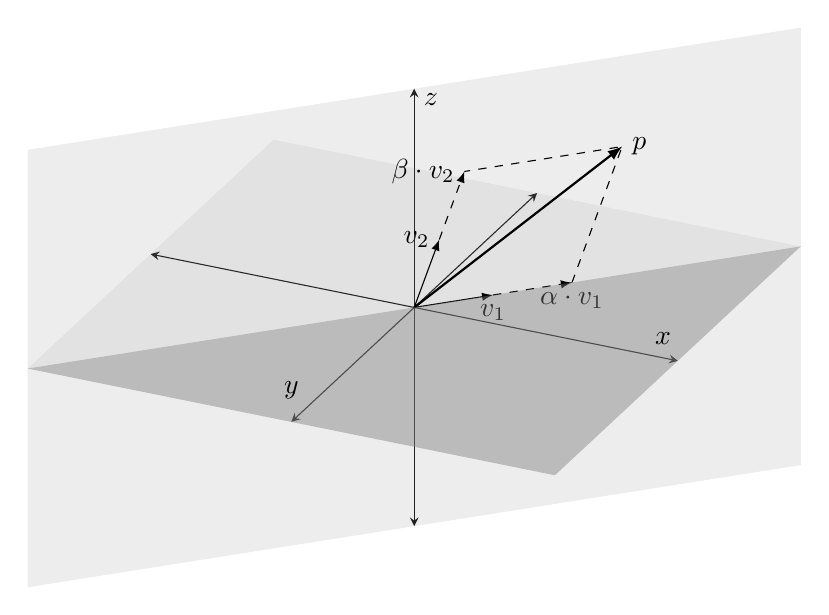
\begin{tikzpicture}
            \begin{axis}[width=11.4cm,height=11.4cm,
            xlabel=$x$, ylabel=\empty, zlabel=$z$,
            xmin=-4.9, xmax=4.9,
            ymin=-4.9, ymax=4.9,
            zmin=-4.9, zmax=4.9,
            axis lines=center,
            %xticklabel=\empty,
            %yticklabel=\empty,
            %zticklabel=\empty,
            axis line style={stealth-stealth},
            ticks=none,
            ]
                \fill[gray,opacity=0.1] (xyz cs:x=-4.9,y=-4.9,z=0) -- (xyz cs:x=4.9,y=-4.9,z=0) -- (xyz cs:x=4.9,y=4.9,z=0) --  (xyz cs:x=-4.9,y=4.9,z=0) -- cycle;
                \fill[gray!70,opacity=0.2] (xyz cs:x=-4.9,y=-4.9,z=-4.9) -- (xyz cs:x=4.9,y=4.9,z=-4.9) -- (xyz cs:x=4.9,y=4.9,z=4.9) --  (xyz cs:x=-4.9,y=-4.9,z=4.9) -- cycle;
                
                \draw[dash pattern=on 3pt off 3pt] (2,2,0) -- (2,4,2) -- (0,2,2);
                
                \draw[-latex,dash pattern=on 3pt off 3pt] (1,1,0) -- (2,2,0) node[below] {$\alpha \cdot \mathbb{v}_1$};
                \draw[-latex] (0,0,0) -- (1,1,0) node[below]{$ \mathbb{v}_1$};

                \draw[-latex,dash pattern=on 3pt off 3pt] (0,1,1) -- (0,2,2) node[left] {$\beta \cdot \mathbb{v}_2$};
                \draw[-latex] (0,0,0) -- (0,1,1) node[left]{$\mathbb{v}_2$};

                \draw[-latex,thick] (0,0,0) -- (2,4,2) node[right]{$\mathbb{p}$};

                %\node [inner sep=2pt,outer sep=0pt] (O) at (axis cs:0,0,0) {};
                %\node [align=center] (origin) at ([xshift=1.5cm,yshift=-1.3cm]O) {$\mathbb{0}$};
                %\draw [shorten <=.1cm,stealth-] (O) to [out=-30,in=160] (origin.west);
                
                \fill[gray,opacity=0.4] (xyz cs:x=-4.9,y=-4.9,z=0) -- (xyz cs:x=4.9,y=-4.9,z=0) -- (xyz cs:x=4.9,y=4.9,z=0) -- cycle;
                \node at (0,-4.9,0.7) {$y$};
            \end{axis}
        \end{tikzpicture}
        \caption{Representación del plano $x - y + z = 0$}
    \end{figure}
\end{example}

\section{Conjuntos linealmente independientes}

\begin{definition}
    Sea $V$ un espacio vectorial sobre $K$. Un subconjunto $S$ del espacio vectorial $V$ se llama linealmente dependiente si existen vectores distintos $\mathbb{v}_1$, $\mathbb{v}_2$, $\dots$, $\mathbb{v}_n$ en $S$ y $a_1$, $a_2$, $\dots$, $a_n$ en $K$ no todos $0$ tales que
    $$a_1 \mathbb{v}_1 + a_2 \mathbb{v}_2 + \cdots + a_n \mathbb{v}_n = \mathbb{0}$$
    En este caso también decimos que los vectores de $S$ son linealmente dependientes. En caso contrario, decimos que los vectores son linealmente independientes y por tanto, $S$ también es linealmente independiente.
\end{definition}

\begin{example}
    En $\RR[2]$, verifique que $\displaystyle \mathbb{v}_1 = \binom{1}{3}$ y $\displaystyle \mathbb{v}_1 = \binom{2}{6}$ son linealmente dependientes. \\
    \solucion Sean $a_1 = 1$ y $\displaystyle a_2 = -\frac{1}{2}$, tenemos\sideFigure[\label{HAHAHAVVAGAGHRRQ}]{
    \begin{center}
        \begin{tikzpicture}
            \draw[thick,-Stealth] (-1,0) -- (4,0) node[below left] {$x$};
            \draw[thick,-Stealth] (0,-1) -- (0,7) node[below left] {$y$};
            \draw[dash pattern=on 3pt off 3pt] (0,3) node[left] {$3$} -- (1,3) -- (1,0) node[below] {$1$};
            \draw[dash pattern=on 3pt off 3pt] (0,6) node[left] {$6$} -- (2,6) -- (2,0) node[below] {$2$};
            \draw[-latex] (0,0) -- (2,6) node [right] {$\mathbb{v}_2$};
            \draw[-latex] (0,0) -- (1,3) node [right] {$\mathbb{v}_1$};
        \end{tikzpicture}
    \end{center}
    }
    \begin{align*}
        a_1\mathbb{v}_1 + a_2\mathbb{v}_2 & = 1 \cdot \binom{1}{3} + \left( -\frac{1}{2} \right) \cdot \binom{2}{6} \\
        & = \binom{1}{3} + \binom{-1}{-3} && \text{por def. de producto escalar} \\
        & = \binom{1+(-1)}{3+(-3)} && \text{por def. de suma en } \RR[2] \\
        & = \binom{0}{0} \\
        & = \mathbb{0}
    \end{align*}
    Además, observemos que
    $$\binom{2}{6} = 2 \cdot \binom{1}{3}$$
    Geométricamente tenemos la figura \ref{HAHAHAVVAGAGHRRQ}.
\end{example}

\begin{theorem}
    Dos vectores en un espacio vectorial son linealmente dependientes si y solo si uno de ellos es un múltiplo escalar del otro. \\
    \demostracion Se deja como ejercicio al lector.
\end{theorem}

\begin{example}
    Verifique que en $\RR[3]$ los vectores $\displaystyle \mathbb{v}_1 = \begin{pmatrix*}[r] 1 \\ -3 \\ 0 \end{pmatrix*}$, $\displaystyle \mathbb{v}_2 = \begin{pmatrix} 3 \\ 0 \\ 4 \end{pmatrix}$ y $\displaystyle \mathbb{v}_3 = \begin{pmatrix*}[r] 11 \\ -6 \\ 12 \end{pmatrix*}$ son linealmente dependientes. \\
    \solucion Hay que demostrar que existen $a_1$, $a_2$, $a_3 \in \RR$ no todos cero, tales que
    $$a_1\mathbb{v}_1 + a_2\mathbb{v}_2 + a_3\mathbb{v}_3 = \mathbb{0}$$
    esto es
    \begin{equation}
        a_1 \cdot \begin{pmatrix*}[r] 1 \\ -3 \\ 0 \end{pmatrix*} + a_2 \cdot \begin{pmatrix} 3 \\ 0 \\ 4 \end{pmatrix} + a_3 \cdot \begin{pmatrix*}[r] 11 \\ -6 \\ 12 \end{pmatrix*} = \begin{pmatrix} 0 \\ 0 \\ 0 \end{pmatrix} \label{ec22}
    \end{equation}
    Veamos que uno de los vectores se puede expresar como combinación lineal de los otros dos, es decir
    $$\begin{pmatrix*}[r] 11 \\ -6 \\ 12 \end{pmatrix*} = a_1 \cdot \begin{pmatrix*}[r] 1 \\ -3 \\ 0 \end{pmatrix*} + a_2 \cdot \begin{pmatrix} 3 \\ 0 \\ 4 \end{pmatrix}$$
    Con $a_1 = 2$, $a_2 = 3$ y $a_3 = -1$, de la ecuación \eqref{ec22}
    \begin{align*}
        2 \cdot \begin{pmatrix*}[r] 1 \\ -3 \\ 0 \end{pmatrix*} + 3 \cdot \begin{pmatrix} 3 \\ 0 \\ 4 \end{pmatrix} - 1 \cdot \begin{pmatrix*}[r] 11 \\ -6 \\ 12 \end{pmatrix*} & = \begin{pmatrix*}[r] 2 \\ -6 \\ 0 \end{pmatrix*} + \begin{pmatrix} 9 \\ 0 \\ 12 \end{pmatrix} + \begin{pmatrix*}[r] -11 \\ 6 \\ -12 \end{pmatrix*} \\
        & = \begin{pmatrix} 2+9-11 \\ -6+0+6 \\ 0+12-12 \end{pmatrix} \\
        & = \begin{pmatrix} 0 \\ 0 \\ 0 \end{pmatrix} = \mathbb{0}
    \end{align*}
    Por tanto, $\mathbb{v}_1$, $\mathbb{v}_2$ y $\mathbb{v}_3$ son vectores linealmente dependientes.
\end{example}

\begin{example}
    Verifique que los vectores $\displaystyle e_1 = \binom{1}{0}$ y $\displaystyle e_2 = \binom{0}{1}$ son linealmente independientes en $\RR[2]$. \\
    \solucion Supongamos que son linealmente dependientes, entonces existen $a_1$, $a_2 \in \RR$ no todos ceros tales que $a_1e_1 + a_2e_2 = \mathbb{0}$. Luego
    \begin{align*}
        \mathbb{0} & = a \cdot \binom{1}{0} + a_2 \cdot \binom{0}{1} \\
        & = \binom{a_1}{0} + \binom{0}{a_2} \\
        & = \binom{a_1}{a_2}
    \end{align*}
    Por tanto, $a_1 = 0$ y $a_2 = 0$, entonces el supuesto es falso y se cumple lo contrario, esto es que $e_1$ y $e_2$ son linealmente independientes.
\end{example}

\begin{example}
    En $\RR[n]$, sean $\displaystyle e_1 = \left( \begin{array}{c} 1 \\ 0 \\ 0 \\ \vdots \\ 0 \\ 0 \end{array} \right)$, $\displaystyle e_2 = \left( \begin{array}{c} 0 \\ 1 \\ 0 \\ \vdots \\ 0 \\ 0 \end{array} \right)$, $\dots$, $\displaystyle e_n = \left( \begin{array}{c} 0 \\ 0 \\ 0 \\ \vdots \\ 0 \\ 1 \end{array} \right)$ son linealmente independientes en $\RR[n]$. \\
    \solucion Se deja como ejercicio al lector probar que dichos vectores son l.i.
\end{example}

\begin{theorem}
    $\RR[n]$ como espacio vectorial sobre $\RR$, tiene a los más $n$ vectores linealmente independientes.
\end{theorem}

\begin{example}
    Considere el espacio vectorial $P_n(x)$ sobre $\RR$. Determine tres vectores en $P_2(x)$ que sean linealmente independientes. \\
    \solucion $\left\{ 1, x, x^2 \right\}$ es l.i, empleando la definición:
    \begin{equation}
        a_1 \cdot 1 + a_2 \cdot x + a_3 \cdot x^2 = \mathbb{0} \label{ec23}
    \end{equation}
    hay que demostrar que $a_1$, $a_2$ y $a_3$ son $0$. De la ecuación \eqref{ec23}
    $$a_1 \cdot 1 + a_2 \cdot x + a_3 \cdot x^2 = 0 \cdot 1 + a \cdot x + 0 \cdot x^2$$
    si y solo si los respectivos coeficientes son iguales, entonces $a_1 = 0$, $a_2 = 0$, $a_3 = 0$. Por lo tanto, $\left\{ 1, x, x^2 \right\}$ es l.i. Determinemos otros tres vectores l.i, sean $\mathbb{v}_1 = 1$, $\mathbb{v}_2 = 1+x$, $\mathbb{v}_3 = 1+x+x^2 \in P_2(x)$. Veamos que son l.i, por la definición sea
    \begin{equation}
        a_1\mathbb{v}_1 + a_2\mathbb{v}_2 + a_3\mathbb{v}_3 = \mathbb{0} \label{ec24}
    \end{equation}
    hay que demostrar que $a_1 = 0$, $a_2 = 0$ y $a_3 = 0$. De la ecuación \eqref{ec24},
    \begin{align*}
        0 \cdot 1 + 0 \cdot x + 0 \cdot x^2 & = a_1 \cdot 1 + a_2 \cdot (1+x) + a_3 \cdot \left( 1+x+x^2 \right) \\
        & = a_1 + (a_2 \cdot 1 + a_2 \cdot x) + \left( a_3 \cdot 1 + a_3 \cdot x + a_3 \cdot x^2 \right) \\
        & = a_1 + a_2 + a_3 + a_2 \cdot x + a_3 \cdot x + a_3 \cdot x^2 \\
        & = (a_1 + a_2 + a_3) + (a_2 + a_3) \cdot x + a_3 \cdot x^2
    \end{align*}
    si y solo si
    \begin{align*}
        a_1 + a_2 + a_3 & = 0 \\
        a_2 + a_3 & = 0 \\
        a_3 & = 0
    \end{align*}
    de donde se sigue que $a_1 = 0$, $a_2 = 0$ y $a_3 = 0$. Por tanto, $\left\{ 1, 1+x, 1+x^2 \right\}$ es l.i.
\end{example}

\section{Base y dimensión}

\begin{definition}
    Sea $V$ un espacio vectorial sobre $K$ y sean $\mathbb{v}_1$, $\mathbb{v}_2$, $\dots$, $\mathbb{v}_n \in V$. Decimos que $\left\{ \mathbb{v}_1, \mathbb{v}_2, \dots, \mathbb{v}_n \right\}$ es una \textbf{base} de $V$ si:
    \begin{enumerate}[label=\roman*)]
        \item $\mathbb{v}_1$, $\mathbb{v}_2$, $\dots$, $\mathbb{v}_n$ son l.i
        \item $V = \Gen \left( \{ \mathbb{v}_1, \mathbb{v}_2, \dots, \mathbb{v}_n \} \right)$
    \end{enumerate}
\end{definition}

\begin{examples}~
    \begin{enumerate}
        \item En $P_n(x)$, $\left\{ 1, x, x^2, \dots, x^n \right\}$ forman una base para $P_n(x)$.
        \item En $\RR[2]$, $\displaystyle e_1 = \binom{1}{0}$ y $\displaystyle e_2 = \binom{0}{1}$ forman una base en $\RR[2]$, pues son l.i y generan a $\RR[2]$.
        \item Para $\RR[n]$, $\displaystyle e_1 = \left( \begin{array}{c} 1 \\ 0 \\ 0 \\ \vdots \\ 0 \\ 0 \end{array} \right)$, $\displaystyle e_2 = \left( \begin{array}{c} 0 \\ 1 \\ 0 \\ \vdots \\ 0 \\ 0 \end{array} \right)$, $\dots$, $\displaystyle e_n = \left( \begin{array}{c} 0 \\ 0 \\ 0 \\ \vdots \\ 0 \\ 1 \end{array} \right)$ forman una base en $\RR[n]$, donde $\{ e_1, e_2, \dots, e_n \}$ se le llama la base canónica de $\RR[n]$.
    \end{enumerate}
\end{examples}

\begin{remark}
    Recordemos que si $A$ es un conjunto no vacío, se define la cardinalidad del conjunto $A$, denotado por $|A|$, como el número de elementos de $A$. Además, se dice que el conjunto $A$ es finito si $|A| < \infty$. En caso contrario, se dice que el conjunto es infinito. Por ejemplo, el conjunto $\NN$.
\end{remark}

\begin{definition}
    Sea $V$ un espacio vectorial sobre $K$. Se llama dimensión del espacio vectorial $V$, a la cardinalidad de la base de $V$, y se denotará por $\Dim V$.
\end{definition}

\begin{examples}~
    \begin{enumerate}
        \item En $P_n(x)$, una base de $P_n(x)$ es $\mathcal{P} = \left\{ 1, x, x^2, \dots, x^n \right\}$. Entonces $\Dim P_n(x) = |\mathcal{P}| = n+1$.
        \item En $\RR[2]$, una base de $\RR[2]$ es $\displaystyle \mathcal{A} = \left\{ \binom{1}{0},  \binom{0}{1} \right\}$. Entonces $\Dim \RR[2] = |\mathcal{A}| = 2$.
        \item En $\RR[n]$, una base de $\RR[n]$ es $\displaystyle \mathcal{B} = \left\{ \left( \begin{array}{c} 1 \\ 0 \\ 0 \\ \vdots \\ 0 \\ 0 \end{array} \right),  \left( \begin{array}{c} 0 \\ 1 \\ 0 \\ \vdots \\ 0 \\ 0 \end{array} \right),  \dots,  \left( \begin{array}{c} 0 \\ 0 \\ 0 \\ \vdots \\ 0 \\ 1 \end{array} \right) \right\}$. Entonces $\Dim \RR[n] = |\mathcal{B}| = n$.
    \end{enumerate}
\end{examples}

\begin{remark}
    Dado el espacio vectorial $V = \left\{ f: \RR \longrightarrow \RR \mid f \text{ es continua} \right\}$, es un espacio vectorial sobre $\RR$ y $\Dim V = \infty$.
\end{remark}

\begin{theorem}
    Sea $V$ un espacio vectorial y $\mathcal{B} = \{ \mathbb{v}_1,  \mathbb{v}_2,  \dots,  \mathbb{v}_n \}$ base de $V$. Entonces todo elemento de $V$ se expresa de manera única a partir de los elementos de la base. Es decir, dado $\mathbb{u} \in V$, existen $a_1$, $a_2$, $\dots$, $a_n \in K$ únicos tales que
    \begin{equation}
        \mathbb{u} = a_1\mathbb{v}_1 + a_2\mathbb{v}_2 + \cdots + a_n\mathbb{v}_n \label{ec25}
    \end{equation}
    \demostracion Supongamos que existen $b_1$, $b_2$, $\dots$, $b_n \in K$ tales que
    \begin{equation}
        \mathbb{u} = b_1\mathbb{v}_1 + b_2\mathbb{v}_2 + \cdots + b_n\mathbb{v}_n \label{ec26}
    \end{equation}
    Se demostrará que $a_i = b_i$, para $i = 1$, $2$, $\dots$, $n$. Sea
    \begin{align*}
        -\mathbb{u} & = (-1) \cdot \mathbb{u} \\
        & = (-1) \cdot (b_1\mathbb{v}_1 + b_2\mathbb{v}_2 + \cdots + b_n\mathbb{v}_n) \\
        & = (-1)b_1\mathbb{v}_1 + (-1)b_2\mathbb{v}_2 + \cdots + (-1)b_n\mathbb{v}_n \\
        & = (-b_1)\mathbb{v}_1 + (-b_2)\mathbb{v}_2 + \cdots + (-b_n)\mathbb{v}_n
    \end{align*}
    Ahora, de las expresiones \eqref{ec25} y \eqref{ec26} tenemos
    \begin{align*}
        \mathbb{0} & = \mathbb{u} + (-\mathbb{u}) \\
        & = a_1\mathbb{v}_1 + a_2\mathbb{v}_2 + \cdots + a_n\mathbb{v}_n + (-b_1)\mathbb{v}_1 + (-b_2)\mathbb{v}_2 + \cdots + (-b_n)\mathbb{v}_n \\
        & = \big(a_1+(-b_1)\big)\mathbb{v}_1 + \big(a_2+(-b_2)\big)\mathbb{v}_2 + \cdots + \big(a_n+(-b_n)\big)\mathbb{v}_n
    \end{align*}
    Entonces $\big(a_1+(-b_1)\big) = 0$, $\big(a_2+(-b_2)\big) = 0$, $\dots$, $\big(a_n+(-b_n)\big) = 0$, ya que $\mathbb{v}_1$, $\mathbb{v}_2$, $\dots$, $\mathbb{v}_n$ son l.i, se sigue que $b_1 = a_1$, $b_2 = a_2$, $\dots$, $b_n = a_n$. Por lo tanto, $\mathbb{u}$ se expresa de manera única.
\end{theorem}

\begin{theorem}
    Sea $V$ un espacio vectorial de dimensión finita $n$, sobre un campo $K$. Entonces dados $\mathbb{v}_1$, $\mathbb{v}_2$, $\dots$, $\mathbb{v}_m \in V$ linealmente independientes, se cumple que $m \leq n$.
\end{theorem}

\begin{remark}
    A los subesapacios distintos a $V$ y $\{ \mathbb{0} \}$ se les llama subespacios propios.
\end{remark}

\begin{observation}
    Todo espacio vectorial admite una base (lema de Zorn).\\
    \demostracion Puede verse una demostración en: Dugundji, James; TOPOLOGY. Allyn and Bacon, Inc. 1975
\end{observation}

\begin{theorem}\label{theorem:teorema1.5.1}
    Sea $V$ un espacio vectorial sobre $K$ con dimension finita $n$, y sea $H \subseteq V$ un subespacio, entonces $\Dim H \leq \Dim V$. \\
    \demostracion Sea $\{ \mathbb{h}_1,  \mathbb{h}_2,  \dots,  \mathbb{h}_k \} \subseteq H$ una base de $H$. Al ser una base, entonces $\mathbb{h}_1$, $\mathbb{h}_2$, $\dots$, $\mathbb{h}_k$ son l.i. Por el teorema anterior, $k \leq n$, de donde se sigue que
    $$\Dim H = k \leq n = \Dim V$$
    Por tanto, $\Dim H \leq \Dim V$.
\end{theorem}

\begin{example}
    Sea $V = \RR[2]$ y sea
    $$\displaystyle H = \left\{ \binom{x}{x} \in \RR[2] \mid x \in \RR \right\}$$
    Sabemos que $H$ es una recta que pasa por $\displaystyle \binom{0}{0}$ y que además $\Dim \RR[2] = 2$. Ahora
    \begin{align*}
        H & = \left\{ \binom{x}{x} \mid x \in \RR \right\} \\
        & = \left\{ x \cdot \binom{1}{1},  x \in \RR \right\}
    \end{align*}
    Esto es
    $$x \cdot \mathbb{h} \text{ con } x \in \RR \quad \text{ y } \quad \mathbb{h} = \binom{1}{1}$$
     Geométricamente tenemos la figura \ref{UABABJABBVAJAHA}. Entonces\sideFigure[\label{UABABJABBVAJAHA}]{
     \begin{tikzpicture}
        \draw[thick,-Stealth] (-1,0) -- (4,0) node[below left] {$x$};
        \draw[thick,-Stealth] (0,-1) -- (0,4) node[below left] {$y$};
        \draw[dash pattern=on 3pt off 3pt] (1,1) -- (3,3) node [above right] {$H$};
        \draw[-latex] (0,0) -- (1,1) node[below right] {$\mathbb{h}$};
        \draw[dash pattern=on 3pt off 3pt] (0,0) -- (-1,-1);
    \end{tikzpicture}
    }
    \begin{align*}
        H & = \left\{ x \cdot \binom{1}{1},  x \in \RR \right\} \\
        & = \Gen \left( \left\{ \binom{1}{1} \right\} \right)
    \end{align*}
    Así $H$ es generado por $\displaystyle \mathbb{h} = \binom{1}{1}$ y además es l.i. Entonces $\displaystyle \left\{ \binom{1}{1} \right\}$ es una base de $H$. Se sigue que $\Dim H = 1$ y $1 \leq 2$, por lo que
    $$\Dim H = 1 \leq 2 = \Dim \RR[2]$$
\end{example}

\begin{theorem}\label{def:n_vectores_base}
    Sea $V$ un espacio vectorial sobre $K$ de dimensión finita $n$, entonces cualquier conjunto de vectores $\mathbb{v}_1$, $\mathbb{v}_2$, $\dots$, $\mathbb{v}_n$ linealmente independientes constituyen una base de $V$. \\
    \demostracion Por hipótesis, tenemos que $\mathbb{v}_1$, $\mathbb{v}_2$, $\dots$, $\mathbb{v}_n$ son l.i. Para demostrar que $\{ \mathbb{v}_1, \mathbb{v}_2, \dots, \mathbb{v}_n \}$ genera a $V$ supongamos lo contrario, esto es que $\{ \mathbb{v}_1, \mathbb{v}_2, \dots, \mathbb{v}_n \}$ no genera a $V$. Entonces existe un $\mathbb{u} \in V$ tal que
    $$\mathbb{u} \notin \Gen(\{ \mathbb{v}_1, \mathbb{v}_2, \dots, \mathbb{v}_n \})$$
    Afirmamos que $\mathbb{u}$ es l.i con $\mathbb{v}_1$, $\mathbb{v}_2$, $\dots$, $\mathbb{v}_n$, es decir, $\mathbb{v}_1$, $\mathbb{v}_2$, $\dots$, $\mathbb{v}_n$, $\mathbb{u}$ son l.i. Así dada la combinación lineal
    \begin{equation}
        a_1\mathbb{v}_1 + a_2\mathbb{v}_2 + \cdots + a_n\mathbb{v}_n + b\mathbb{u} = \mathbb{0} \label{ec27}
    \end{equation}
    Afirmamos que $b = 0$. Supongamos lo contrario, es decir, $b \neq 0$. De la ecuación \eqref{ec27},
    $$a_1\mathbb{v}_1 + a_2\mathbb{v}_2 + \cdots + a_n\mathbb{v}_n + \mathbb{0} = \mathbb{0} + (-b\mathbb{u})$$
    Multiplicando por el inverso multiplicativo de $-b \in K$, es decir, $\displaystyle (-b)^{-1} = - \frac{1}{b}$, obtenemos
    $$\left(-\frac{a_1}{b}\right)\mathbb{v}_1 + \left(-\frac{a_2}{b}\right)\mathbb{v}_2 + \cdots + \left(-\frac{a_n}{b}\right)\mathbb{v}_n = \mathbb{u} \in \Gen(\{ \mathbb{v}_1, \mathbb{v}_2, \dots, \mathbb{v}_n \})$$
    lo cual es una contradicción, pues $\mathbb{u} \notin \Gen(\{ \mathbb{v}_1, \mathbb{v}_2, \dots, \mathbb{v}_n \})$. Por lo tanto, $b = 0$. Sustituyendo en la ecuación \eqref{ec27}
    $$a_1\mathbb{v}_1 + a_2\mathbb{v}_2 + \cdots + a_n\mathbb{v}_n + 0 \cdot \mathbb{u} = \mathbb{0}$$
    Así
    $$a_1\mathbb{v}_1 + a_2\mathbb{v}_2 + \cdots + a_n\mathbb{v}_n = \mathbb{0}$$
    Entonces
    $$a_1 = a_2 = \cdots = a_n = 0$$
    ya que $\mathbb{v}_1$, $\mathbb{v}_2$, $\dots$, $\mathbb{v}_n$ son l.i. Por el teorema \ref{theorem:teorema1.5.1},
    $$n + 1 \leq \Dim V = n$$
    lo cual es una contradicción. Por lo tanto $\{ \mathbb{v}_1,  \mathbb{v}_2,  \dots,  \mathbb{v}_n \}$ genera a $V$.
\end{theorem}

\begin{example}
    Sabemos que la dimensión de $P_2(x) = 3$. Entonces el conjunto $\left\{ 1-x^2,  x \right\}$ no puede ser una base de $P_2(x)$, pues tendríamos a lo más dos vectores linealmente independientes y $2 < 3 = \Dim P_2(x)$. Por tanto, por el teorema anterior $\left\{ 1-x^2,  x \right\}$ no es una base de $P_2(x)$.
\end{example}

\begin{theorem}
    Si $\left\{ \mathbb{u}_1, \mathbb{u}_2, \dots, \mathbb{u}_m \right\}$ y $\left\{ \mathbb{v}_1, \mathbb{v}_2, \dots, \mathbb{v}_n \right\}$ son dos bases de un espacio vectorial $V$ de dimensión finita, entonces $m = n$. Es decir, cualesquiera dos bases de un espacio vectorial $V$ de dimensión finita tienen el mismo número de vectores. \\
    \demostracion Sea $S_1 = \left\{ \mathbb{u}_1, \mathbb{u}_2, \dots, \mathbb{u}_m \right\}$ y $S_2 = \left\{ \mathbb{v}_1, \mathbb{v}_2, \dots, \mathbb{v}_n \right\}$ dos bases de $V$. Es necesario demostrar que $m = n$. Para ello, se procede a mostrar que si $m > n$, entonces $S_1$ es linealmente independiente, lo cual contradice la premisa de que $S_1$ es una base. Esto establecerá que $m \leq n$. De manera análoga, se demuestra que $n \leq m$, lo que concluye el teorema. Por lo tanto, es suficiente demostrar que si $m > n$, entonces $S_1$ es un conjunto linealmente dependiente. Dado que $S_2$ es una base, cada vector $\mathbb{u}_i$ puede expresarse como una combinación lineal de los vectores $\mathbb{v}_j$. Por consiguiente, se tiene
    \begin{equation}
        \begin{aligned}
           \mathbb{u}_1 & = a_{11} \mathbb{v}_1 + a_{12} \mathbb{v}_2 + \cdots + a_{1n} \mathbb{v}_n \\
            \mathbb{u}_2 & = a_{21} \mathbb{v}_1 + a_{22} \mathbb{v}_2 + \cdots + a_{2n} \mathbb{v}_n \\
            & \vdots \\
            \mathbb{u}_m & = a_{m1} \mathbb{v}_1 + a_{m2} \mathbb{v}_2 + \cdots + a_{mn} \mathbb{v}_n
        \end{aligned} \label{ECUACION5.5.1}
    \end{equation}
    Para demostrar que $S_1$ es linealmente dependiente, se deben encontrar escalares $c_1$, $c_2$, $\dots$, $c_m$ no todos cero, tales que
    \begin{equation}
        c_1\mathbb{u}_1 + c_2\mathbb{u}_2 + \cdots + c_m\mathbb{u}_m = \mathbb{0} \label{ECUACION5.5.2}
    \end{equation}
    Sustituyendo \eqref{ECUACION5.5.1} en \eqref{ECUACION5.5.2} se obtiene
    $$c_1\left( a_{11} \mathbb{v}_1 + a_{12} \mathbb{v}_2 + \cdots + a_{1n} \mathbb{v}_n \right) + c_2\left( a_{21} \mathbb{v}_1 + a_{22} \mathbb{v}_2 + \cdots + a_{2n} \mathbb{v}_n \right) + \cdots + c_m\left( a_{m1} \mathbb{v}_1 + a_{m2} \mathbb{v}_2 + \cdots + a_{mn} \mathbb{v}_n \right) = \mathbb{0}$$
    Es decir,
    $$\left( a_{11}c_1 + a_{21}c_2 + \cdots + a_{m1}c_m \right)\mathbb{v}_1 + \left( a_{12}c_1 + a_{22}c_2 + \cdots + a_{m2}c_m \right)\mathbb{v}_2 + \cdots + \left( a_{1n}c_1 + a_{2n}c_2 + \cdots + a_{mn}c_m \right)\mathbb{v}_m = \mathbb{0}$$
    Pero $\mathbb{v}_1$, $\mathbb{v}_2$, $\dots$, $\mathbb{v}_n$ son linealmente independientes, entonces
    \begin{align*}
        a_{11}c_1 + a_{21}c_2 + \cdots + a_{m1}c_m & = 0 \\
        a_{12}c_1 + a_{22}c_2 + \cdots + a_{m2}c_m & = 0 \\
        & \vdots \\
        a_{1n}c_1 + a_{2n}c_2 + \cdots + a_{mn}c_m & = 0
    \end{align*}
    Nótese que el sistema anterior constituye un sistema de $n$ ecuaciones con $m$ incógnitas, lo que implica que $m > n$. Por lo tanto, el sistema tiene un número infinito de soluciones. De esta manera, existen escalares $c_1$, $c_2$, $\dots$, $c_m$, no todos nulos, tales que la ecuación \eqref{ECUACION5.5.2} se satisface, lo que implica que $S_1$ es un conjunto linealmente dependiente. Esta contradicción demuestra que $m \leq n$. Al intercambiar los roles de $S_1$ y $S_2$, se demuestra que $n \leq m$, lo que completa la prueba.
\end{theorem}

\begin{adjustwidth}{-2.15cm}{-\wholeMargin -3.5cm}
    \begin{tcolorbox}[
        theorem style=change break,
        enhanced,
        breakable,
        boxrule=0pt,
        frame hidden,
        left = 2cm,
        right = 2cm,
        top=6mm,
        bottom=1mm,
        colback=gray!20,
        coltitle=black,
        attach title to upper={\ },
        sharp corners,
        title = Algunas observaciones:,
        fonttitle=\sffamily\bfseries\LARGE,
        fontupper=\normalsize
    ]
        \begin{tikzpicture}[remember picture,overlay] \filldraw[gray!20] (current page.south west) rectangle ($(current page.south east) + (0,3)$); \end{tikzpicture}
        \begin{multicols}{2}
            \hspace*{5.5mm}En este capítulo hemos explorado los fundamentos de los espacios vectoriales reales. Es importante destacar que nos hemos enfocado exclusivamente en el estudio de vectores y operaciones definidas sobre ellos en el contexto de números reales. Sin embargo, es crucial reconocer que todo lo que hemos aprendido en este capítulo se puede generalizar y extender al ámbito de los espacios vectoriales complejos. A medida que avanzamos hacia el capítulo \ref{chap:espacios_complejos}, exploraremos cómo los números complejos enriquecen nuestra comprensión de los espacios vectoriales y amplían nuestras capacidades de modelado y resolución de problemas.
            
            \hspace*{5.5mm}Es importante destacar que $\CC[n]$, el espacio de los vectores $n$-dimensionales con coeficientes complejos, constituye un espacio vectorial sobre los números complejos $\CC$. Demostraremos en el capítulo \ref{chap:espacios_complejos} que las propiedades fundamentales de los espacios vectoriales se mantienen cuando trabajamos con coeficientes complejos. Así, aunque nos hemos centrado en los espacios vectoriales reales en este capítulo, es importante reconocer la relevancia y la conexión entre ambos ámbitos. La extensión de nuestros conocimientos a los espacios vectoriales complejos nos permitirá abordar una gama aún más amplia de problemas y aplicaciones en matemáticas y disciplinas relacionadas.
            
            \hspace*{5.5mm}Para aquellos lectores que no estén familiarizados con los números complejos, se recomienda consultar el \hyperref[chap:numeros-complejos]{Apéndice B}, donde se proporciona una introducción detallada y accesible a este campo. En este apéndice, se abordan los conceptos básicos de los números complejos, incluyendo operaciones fundamentales como la suma, la resta, la multiplicación y la división; así como propiedades importantes como el conjugado y el módulo.
        \end{multicols}
    \end{tcolorbox}
\end{adjustwidth}

\newpage

\section{Ejercicios}

\noindent
De los problemas 1 al 15 determine si el conjunto dado es un espacio vectorial. De no ser así proporcione una lista de los axiomas que no se cumplen.
\begin{enumerate}
    \item El conjunto de números naturales $\NN$ como vectores, el conjunto de números naturales $\NN$ como escalares y la operación de multiplicación para números naturales.
    \item El conjunto de números naturales $\NN$ como vectores, el conjunto de números naturales $\NN$ como escalares, la operación de suma para números naturales y la multiplicación entre números naturales para la operación de multiplicación de escalar y vector.
    \item El conjunto de números enteros $\ZZ$ como vectores, el conjunto de números naturales $\NN$ como escalares, la operación de suma para números enteros y la multiplicación entre números enteros para la operación de multiplicación de escalar y vector.
    \item $\left\{ \begin{pmatrix} x \\ y \end{pmatrix} \mid y \leq 0 \text{ donde } x, y \in \RR \right\}$ con la suma de vectores y multiplicación por un escalar usuales.
    \item Los vectores en el plano que está en el primer cuadrante.
    \item El conjunto de vectores en $\RR[2]$ de la forma $\begin{pmatrix} x \\ x \end{pmatrix}$.
    \item El conjunto de vectores los números racionales $\QQ$ con la operación de suma, el conjunto de escalares los números enteros $\ZZ$ y la operación de multiplicación de escalar y vector la multiplicación usual.
    \item El conjunto de polinomios de grado menor o igual a $n$ con término constante cero.
    \item El conjunto de polinomios de grado menor o igual a $n$ con término constante $a_{0}$ positivo.
    \item El conjunto de polinomios de grado menor o igual a $n$ con término constante $a_{0}$ negativo.
    \item El conjunto de funciones continuas de valores reales definidas en $[0, 1]$ con $f(0) = 0$ y $f(1) = 0$ bajo las operaciones del ejemplo \ref{ejemplo5.1.8}.
    \item El conjunto de puntos en $\RR[3]$ que se encuentran sobre una recta que pasa por el origen.
    \item El conjunto de puntos en $\RR[3]$ que se encuentran sobre la recta $x = t+1$, $y = 2t$, $z = t-1$.
    \item El conjunto de funciones diferenciables definidas en $[0, 1]$ con las operaciones del ejemplo \ref{ejemplo5.1.8}.
    \item El conjunto de números reales de la forma $a+b \sqrt{2}$, donde $a$ y $b$ son números racionales, bajo la suma de números reales usual y la multiplicación por un escalar definida sólo para escalares racionales.
\end{enumerate}
De los problemas 16 al 34 determine si el subconjunto dado $H$ del espacio vectorial $V$ es un subespacio de $V$.
\begin{enumerate}[resume]
    \item $V=\RR[2]$; $H=\left\{ \begin{pmatrix} x \\ y \end{pmatrix} \mid x=3, y \in \RR \right\}$
    \item $V=\RR[2]$; $H=\left\{ \begin{pmatrix} x \\ y \end{pmatrix} \mid y \geq 0 \right\}$\newpage
    \item $V=\RR[2]$; $H=\left\{ \begin{pmatrix} x \\ y \end{pmatrix} \mid x=y \right\}$
    \item $V=\RR[2]$; $H=\left\{ \begin{pmatrix} x \\ y \end{pmatrix} \mid y=2 x \right\}$
    \item $V=\RR[3]$; $H = \operatorname{el~plano} x y$
    \item $V=\RR[2]$; $H=\left\{ \begin{pmatrix} x \\ y \end{pmatrix} \mid x^{2}+y^{2} \leq 1\right\}$
    \item $V=\RR[2]$; $H=\left\{ \begin{pmatrix} x \\ y \end{pmatrix} \mid x^{2}+y^{3}<1\right\}$
    \item $V=\RR$; $H=\QQ$
    \item $V=P_{n}$; $H=\left\{p \in P_{n}\mid p(0)=0\right.$ y $\left.p^{\prime}(0)=0\right\}$
    \item $V=P_{4}$; $H=\left\{p \in P_{4}\mid p(0)=0\right\}$
    \item $V=P_{n}$; $H=\left\{p \in P_{n}\mid p(0)=0\right\}$
    \item $V=P_{n}$; $H=\left\{p \in P_{n}\mid p(0)=1\right\}$
    \item $V=C[0,1]$; $H=\{f \in C[0,1]\mid f(0)=f(1)=0\}$
    \item $V=C[0,1]$; $H=\{f \in C[0,1]\mid f(0)=2\}$
    \item $V=C^{1}[0,1]$; $H=\left\{f \in C^{1}[0,1]\mid f^{\prime}(0)=0\right\}$
    \item $V=C[a, b]$; donde $a$, $b \in \RR$ y $a<b$; $\displaystyle H=\left\{f \in C[a, b]\mid \int_{a}^{b} f(x) d x=0\right\}$
    \item $V=C[a, b]$; $\displaystyle H=\left\{f \in C[a, b]\mid \int_{a}^{b} f(x) d x=1\right\}$
    \item $V=C[a, b]$; $\displaystyle H=\left\{f \in C[a, b]\mid \int_{a}^{b} f^{2}(x) d x=0\right\}$
    \item Sea $H=\left\{ \begin{pmatrix} x \\ y \\ z \\ w \end{pmatrix} \mid a x+b y+c z+d w=0\right\}$, donde $a, b, c$ y $d$ son números reales, no todos cero. Demuestre que $H$ es un subespacio propio de $\RR[4]$. $H$ se llama un hiperplano en $\RR[4]$ que pasa por el origen.
\end{enumerate}
De los problemas 35 al 52 determine si el conjunto dado de vectores genera el espacio vectorial dado.
\begin{enumerate}[resume]
    \item En $ \RR[2]$: $\begin{pmatrix} 2 \\ 10 \end{pmatrix}, \begin{pmatrix} 10 \\ 8 \end{pmatrix}$
    \item En $ \RR[2]$: $\begin{pmatrix} 1 \\ 2 \end{pmatrix}, \begin{pmatrix} 3 \\ 4 \end{pmatrix}$
    \item En $ \RR[2]$: $\begin{pmatrix} 1 \\ 1 \end{pmatrix}, \begin{pmatrix} 2 \\ 1 \end{pmatrix}, \begin{pmatrix} 2 \\ 2 \end{pmatrix}$
    \item En $\RR[2]$: $\begin{pmatrix} 0 \\ 1 \end{pmatrix}, \begin{pmatrix} 3 \\ 4 \end{pmatrix}, \begin{pmatrix*}[r] -1 \\ -2 \end{pmatrix*}$
    \item En $ \RR[2]$: $\begin{pmatrix*}[r] -12 \\ 5 \end{pmatrix*}, \begin{pmatrix*}[r] -3 \\ 0 \end{pmatrix*}, \begin{pmatrix*}[r] 4 \\ -8 \end{pmatrix*}$\newpage
    \item En $\RR[2]$: $\begin{pmatrix*}[r] -6 \\ 5 \end{pmatrix*}, \begin{pmatrix} 7 \\ 9 \end{pmatrix}, \begin{pmatrix*}[r] 7 \\ -12 \end{pmatrix*}, \begin{pmatrix*}[r] -10 \\ 6 \end{pmatrix*}$
    \item En $ \RR[2]$: $\begin{pmatrix} 1 \\ 1 \end{pmatrix}, \begin{pmatrix} 2 \\ 2 \end{pmatrix}, \begin{pmatrix} 5 \\ 5 \end{pmatrix}$
    \item En $\RR[3]$: $\begin{pmatrix} 1 \\ 2 \\ 3 \end{pmatrix}, \begin{pmatrix*}[r] -1 \\ 2 \\ 3 \end{pmatrix*}, \begin{pmatrix} 5 \\ 2 \\ 3 \end{pmatrix}$
    \item En $\RR[3]$: $\begin{pmatrix} 0 \\ 5 \\ 1 \end{pmatrix}, \begin{pmatrix*}[r] 0 \\ -1 \\ 3 \end{pmatrix*}, \begin{pmatrix*}[r] -1 \\ -1 \\ 5 \end{pmatrix*}$
    \item En $\RR[3]$: $\begin{pmatrix} 1 \\ 1 \\ 1 \end{pmatrix}, \begin{pmatrix} 0 \\ 1 \\ 1 \end{pmatrix}, \begin{pmatrix} 0 \\ 0 \\ 1 \end{pmatrix}$
    \item En $\RR[3]$: $\begin{pmatrix} 2 \\ 0 \\ 1 \end{pmatrix}, \begin{pmatrix} 3 \\ 1 \\ 2 \end{pmatrix}, \begin{pmatrix} 1 \\ 1 \\ 1 \end{pmatrix}, \begin{pmatrix} 7 \\ 3 \\ 5 \end{pmatrix}$
    \item En $\RR[3]$: $\begin{pmatrix*}[r] -7 \\ -6 \\ 9 \end{pmatrix*}, \begin{pmatrix*}[r] 14 \\ -6 \\ 18 \end{pmatrix*}, \begin{pmatrix} 7 \\ 0 \\ 3 \end{pmatrix}, \begin{pmatrix*}[r] 35 \\ 18 \\ -21 \end{pmatrix*}$
    \item En $ \RR[3]$: $\begin{pmatrix*}[r] 4 \\ 4 \\ -6 \end{pmatrix*}, \begin{pmatrix*}[r] -8 \\ 4 \\ -24 \end{pmatrix*}, \begin{pmatrix*}[r] -4 \\ 0 \\ -6 \end{pmatrix*}$
    \item En $P_{2}$: $1-x, 3-x^{2}$
    \item En $P_{2}$: $1-x, 3-x^{2}, x$
    \item En $P_{2}$: $x^{2}+1 ; x^{2}-1 ; x+6$
    \item En $P_{2}$: $-12 x+5 x^{2},-9-27 x+8 x^{2},-3-5 x+x^{2}$
    \item En $P_{2}$: $-10+3 x+11 x^{2}, 10+9 x-4 x^{2}, 5+x+4 x^{2}$
\end{enumerate}
De los problemas 53 al 60 describa el espacio generado por los vectores.
\begin{enumerate}[resume]
    \item $\begin{pmatrix*}[r] -6 \\ 3 \end{pmatrix*}, \begin{pmatrix*}[r] -11 \\ 5 \end{pmatrix*}$
    \item $\begin{pmatrix*}[r] -5 \\ -8 \end{pmatrix*}, \begin{pmatrix*}[r] -4 \\ -8 \end{pmatrix*}, \begin{pmatrix*}[r] 10 \\ -5 \end{pmatrix*}$
    \item $\begin{pmatrix*}[r] -12 \\ -16 \end{pmatrix*}, \begin{pmatrix} 6 \\ 8 \end{pmatrix}, \begin{pmatrix} 18 \\ 24 \end{pmatrix}$
    \item $\begin{pmatrix*}[r] 20 \\ -23 \\ -8 \end{pmatrix*}, \begin{pmatrix*}[r] 2 \\ 7 \\ -2 \end{pmatrix*}, \begin{pmatrix*}[r] 8 \\ -3 \\ -4 \end{pmatrix*}, \begin{pmatrix*}[r] -2 \\ 24 \\ -2 \end{pmatrix*}$
    \item $\begin{pmatrix*}[r] -3 \\ -3 \\ -2 \end{pmatrix*}, \begin{pmatrix*}[r] -2 \\ 4 \\ -8 \end{pmatrix*}, \begin{pmatrix*}[r] 6 \\ -6 \\ 12 \end{pmatrix*}$
    \item $\begin{pmatrix*}[r] -9 \\ 8 \\ -4 \end{pmatrix*}, \begin{pmatrix} 39 \\ 20 \\ 38 \end{pmatrix}, \begin{pmatrix*}[r] -34 \\ 12 \\ -22 \end{pmatrix*}, \begin{pmatrix} 7 \\ 12 \\ 10 \end{pmatrix}$\newpage
    \item $\begin{pmatrix*}[r] 2 \\ -1 \\ -1 \end{pmatrix*}, \begin{pmatrix*}[r] -4 \\ 2 \\ 2 \end{pmatrix*}, \begin{pmatrix*}[r] 6 \\ -3 \\ -3 \end{pmatrix*}$
    \item $\begin{pmatrix*}[r] -6 \\ 3 \\ 9 \\ -12 \end{pmatrix*}, \begin{pmatrix*}[r] 9 \\ 12 \\ -18 \\ 6 \end{pmatrix*}, \begin{pmatrix*}[r] -23 \\ 25 \\ 25 \\ -56 \end{pmatrix*}, \begin{pmatrix*}[r] -1 \\ 6 \\ 0 \\ -6 \end{pmatrix*}$
    \item Demuestre que dos polinomios de grado menor o igual a dos, no pueden generar $P_{2}$.
    \item Si $p_{1}, p_{2}, \dots, p_{m}$ genera $P_{m}$, demuestre que $m \geq n+1$.
    \item Demuestre que si $\mathbb{u}$ y $\mathbb{v}$ están en $\Gen \left( \left\{\mathbb{v}_{1}, \mathbb{v}_{2}, \dots, \mathbb{v}_{k}\right\} \right)$, entonces $\mathbb{u}+\mathbb{v}$ y $\alpha \mathbb{u}$ están en $\Gen \left( \left\{\mathbb{v}_{1}, \mathbb{v}_{2}, \dots, \mathbb{v}_{k}\right\} \right)$.
    \item Demuestre que el conjunto infinito $\left\{1, x, x^{2}, x^{3}, \dots\right\}$ genera $P$, el espacio vectorial de polinomios.
    \item Sea $H$ un subespacio de $V$ que contiene a $\mathbb{v}_{1}, \mathbb{v}_{2}, \dots, \mathbb{v}_{n}$. Demuestre que $\Gen \left( \left\{\mathbb{v}_{1}, \mathbb{v}_{2}, \dots, \mathbb{v}_{n}\right\} \right) \subseteq H$. Es decir, $\Gen \left( \left\{\mathbb{v}_{1}, \mathbb{v}_{2}, \dots, \mathbb{v}_{n}\right\} \right)$ es el subespacio más pequeño de $V$ que contiene a $\mathbb{v}_{1}, \mathbb{v}_{2}, \dots, \mathbb{v}_{n}$.
    \item Sean $\mathbb{v}_{1}=\begin{pmatrix} x_{1} \\ y_{1} \\ z_{1} \end{pmatrix}$ y $\mathbb{v}_{2}=\begin{pmatrix} x_{2} \\ y_{2} \\ z_{2} \end{pmatrix}$ en $\RR[3]$. Demuestre que si $\mathbb{v}_{2}=c \mathbb{v}_{1}$, entonces $\Gen \left\{\mathbb{v}_{1}, \mathbb{v}_{2}\right\}$ es una recta que pasa por el origen.
    \item En el problema anterior suponga que $\mathbb{v}_{1}$ y $\mathbb{v}_{2}$ no son paralelos. Demuestre que $H= \Gen \left\{\mathbb{v}_{1}, \mathbb{v}_{2}\right\}$ es un plano que pasa por el origen. ¿Cuál es la ecuación del plano?
\end{enumerate}
De los problemas 68 al 89 determine si el conjunto de vectores dado es linealmente dependiente o independiente.
\begin{multienumerate}\setcounter{multienumi}{67}
    \mitemxx{$\begin{pmatrix*}[r]9 \\ -8\end{pmatrix*},\begin{pmatrix*}[r]-11 \\ -3\end{pmatrix*}$}{$\begin{pmatrix*}1 \\ 2\end{pmatrix*},\begin{pmatrix*}-1 \\ -3\end{pmatrix*}$}
    \mitemxx{$\begin{pmatrix*}[r]2 \\ -1 \\ 4\end{pmatrix*},\begin{pmatrix*}[r]4 \\ -2 \\ 7\end{pmatrix*}$}{$\begin{pmatrix*}[r]-6 \\ 1\end{pmatrix*},\begin{pmatrix*}[r]12 \\ -2\end{pmatrix*}$}
    \mitemxx{$\begin{pmatrix*}[r]2 \\ -1 \\ 4\end{pmatrix*},\begin{pmatrix*}[r]4 \\ -2 \\ 8\end{pmatrix*}$}{$\begin{pmatrix*}[r]-2 \\ 3\end{pmatrix*},\begin{pmatrix*}4 \\ 7\end{pmatrix*}$}
    \mitemxx{$\begin{pmatrix*}1 \\ 0 \\ 0\end{pmatrix*},\begin{pmatrix*}0 \\ 1 \\ 1\end{pmatrix*}$}{$\begin{pmatrix*}[r]-10 \\ -6\end{pmatrix*},\begin{pmatrix*}[r]10 \\ -6\end{pmatrix*},\begin{pmatrix*}5 \\ 9\end{pmatrix*}$}
    \mitemxx{$\begin{pmatrix*}1 \\ 0 \\ 1\end{pmatrix*},\begin{pmatrix*}0 \\ 1 \\ 1\end{pmatrix*},\begin{pmatrix*}1 \\ 1 \\ 0\end{pmatrix*}$}{$\begin{pmatrix*}1 \\ 0 \\ 1\end{pmatrix*},\begin{pmatrix*}0 \\ 1 \\ 0\end{pmatrix*},\begin{pmatrix*}0 \\ 0 \\ 1\end{pmatrix*}$}
    \mitemxx{$\begin{pmatrix*}[r]8 \\ -7 \\ -8\end{pmatrix*},\begin{pmatrix*}[r]-11 \\ -12 \\ -7\end{pmatrix*},\begin{pmatrix*}[r]12 \\ -3 \\ 7\end{pmatrix*}$}{$\begin{pmatrix*}1 \\ 2 \\ 3\end{pmatrix*},\begin{pmatrix*}[r]-1 \\ 1 \\ -1\end{pmatrix*},\begin{pmatrix*}[r]4 \\ -1 \\ 1\end{pmatrix*}$}
    \mitemxx{$\begin{pmatrix*}[r]-3 \\ 4 \\ 2\end{pmatrix*},\begin{pmatrix*}[r]7 \\ -1 \\ 3\end{pmatrix*},\begin{pmatrix*}1 \\ 1 \\ 8\end{pmatrix*}$}{$\begin{pmatrix*}[r]-1 \\ 0 \\ 11\end{pmatrix*},\begin{pmatrix*}[r]7 \\ -20 \\ -29\end{pmatrix*},\begin{pmatrix*}[r]1 \\ -5 \\ 1\end{pmatrix*}$}
    \mitemxx{En $P_{2}$: $1-x, x$}{En $P_{2}$: $-x, x^{2}-2 x, 3 x+5 x^{2}$}
    \mitemx{En $P_2$: $-3-2 x-11 x^{2},-39-6 x-3 x^{2},-12-9 x^{2}, 20-4 x+5 x^{2}$}
    \newpage
    \mitemx{En $P_{4}$: $x-1,(x-1)(x-2),(x-1)(x-2)(x-3), x^{4}$}
    \mitemxx{En $P_{2}$: $x, x^{2}-x, x^{3}-x$}{En $C[0,1]$: $e^{x}, e^{-x}$}
    \mitemxx{En $C[0,1]$: $\sen x, \cos x$}{En $C[0,1]$: $x, \sqrt{x}, \sqrt[3]{x}$}
\end{multienumerate}
\begin{enumerate}[start=90]
    \item Determine una condición sobre los números $a, b, c$ y $d$ tal que los vectores $\begin{pmatrix*}a \\ b\end{pmatrix*}$ y $\begin{pmatrix*}c \\ d\end{pmatrix*}$ sean linealmente dependientes.
    \item Encuentre una condición sobre los números $a_{i j}$ tal que los vectores $\begin{pmatrix*}a_{11} \\ a_{21} \\ a_{31}\end{pmatrix*},\begin{pmatrix*}a_{12} \\ a_{22} \\ a_{32}\end{pmatrix*}$ y $\begin{pmatrix*}a_{13} \\ a_{23} \\ a_{33}\end{pmatrix*}$ sean linealmente independientes.
    \item ¿Para qué valor(es) de $\alpha$ serán linealmente dependientes los vectores $\begin{pmatrix*}1 \\ 2 \\ 3\end{pmatrix*},\begin{pmatrix*}[r]2 \\ -1 \\ 4\end{pmatrix*},\begin{pmatrix*}3 \\ \alpha \\ 4\end{pmatrix*}$?
    \item ¿Para qué valor(es) de $\alpha$ serán linealmente dependientes los vectores $\begin{pmatrix*}[r]2 \\ -3 \\ 1\end{pmatrix*},\begin{pmatrix*}[r]-4 \\ 6 \\ -2\end{pmatrix*},\begin{pmatrix*}\alpha \\ 1 \\ 2\end{pmatrix*}$?
    \item ¿Para qué valor(es) de $\alpha$ serán linealmente dependientes los vectores $\begin{pmatrix*}3 \\ 2 \\ 1\end{pmatrix*},\begin{pmatrix*}-2 \\ -1 \\ -1\end{pmatrix*},\begin{pmatrix*}\alpha \\ 5 \\ 2\end{pmatrix*}$?
    \item ¿Para qué valor(es) de $\alpha$ y $\beta$ serán linealmente independientes los vectores $\begin{pmatrix*}3 \\ 2 \\ 1\end{pmatrix*},\begin{pmatrix*}[r]-2 \\ -1 \\ \beta\end{pmatrix*},\begin{pmatrix*}\alpha \\ 5 \\ 2\end{pmatrix*}$?
    \item Demuestre que si los vectores $\mathbb{v}_{1}, \mathbb{v}_{2}, \dots, \mathbb{v}_{n}$ son linealmente dependientes en $\RR[m]$, con $m<n$, y si $\mathbb{v}_{n+1}$ es cualquier otro vector en $\RR[m]$, entonces el conjunto $\mathbb{v}_{1}, \mathbb{v}_{2}, \dots, \mathbb{v}_{n}, \mathbb{v}_{n+1}$ es linealmente dependiente.
    \item Demuestre que si $\mathbb{v}_{1}, \mathbb{v}_{2}, \dots, \mathbb{v}_{n}$ ($n \geq 2$) son linealmente independientes, entonces también lo son $\mathbb{v}_{1}, \mathbb{v}_{2}, \dots, \mathbb{v}_{k}$, donde $k<n$.
    \item Demuestre que cualesquiera cuatro polinomios en $P_{2}$ son linealmente dependientes.
    \item Demuestre que dos polinomios no pueden generar a $P_{2}$.
    \item Demuestre que cualesquiera $n+2$ polinomios en $P_{n}$ son linealmente dependientes.
    \item Demuestre que cualquier subconjunto de un conjunto de vectores linealmente independientes es linealmente independiente.
    \item Sean $S_{1}$ y $S_{2}$ dos conjuntos finitos linealmente independientes en un espacio vectorial $V$. Demuestre que $S_{1} \cap S_{2}$ es un conjunto linealmente independiente.
    \item Sea $S=\left\{\mathbb{v}_{1}, \mathbb{v}_{2}, \dots, \mathbb{v}_{n}\right\}$ un conjunto linealmente independiente de vectores diferentes de cero en un espacio vectorial $V$. Demuestre que al menos uno de los vectores en $S$ se puede escribir como una combinación lineal de los vectores que le preceden. Es decir, demuestre que existe un entero $k \leq n$ y escalares $\alpha_{1}, \alpha_{2}, \dots, \alpha_{k-1}$ tales que $\mathbb{v}_{k}=\alpha_{1} \mathbb{v}_{1}, \alpha_{2} \mathbb{v}_{2}, \dots$, $\alpha_{k-1} \mathbb{v}_{k-1}$.\newpage
    \item Sea $\left\{\mathbb{v}_{1}, \mathbb{v}_{2}, \dots, \mathbb{v}_{n}\right\}$ un conjunto linealmente independiente. Demuestre que los vectores $\mathbb{v}_{1}, \mathbb{v}_{1}+\mathbb{v}_{2}, \mathbb{v}_{1}+\mathbb{v}_{2}+\mathbb{v}_{3}, \dots, \mathbb{v}_{1}+\mathbb{v}_{2}+\cdots+\mathbb{v}_{n}$ son linealmente independientes.
    \item Sea $\left\{\mathbb{v}_{1}, \mathbb{v}_{2}, \dots, \mathbb{v}_{n}\right\}$ un conjunto de vectores que tiene la propiedad de que el conjunto $\left\{\mathbb{v}_{i}, \mathbb{v}_{j}\right\}$ es linealmente dependiente cuando $i \neq j$. Demuestre que cada vector del conjunto es un múltiplo de un solo vector de ese conjunto.
    \item Suponga que $\mathbb{u}, \mathbb{v}$ y $\mathbb{w}$, son linealmente independientes. Pruebe o desapruebe: $\mathbb{u}+\mathbb{v}, \mathbb{u}+\mathbb{w}$ y $\mathbb{u}+\mathbb{w}$ son linealmente independientes.
    \item Sea $\left\{\mathbb{v}_{1}, \mathbb{v}_{2}, \dots, \mathbb{v}_{n}\right\}$ un conjunto linealmente independiente y suponga que $\mathbb{v} \notin \Gen \left( \left\{\mathbb{v}_{1}, \mathbb{v}_{2}, \dots, \mathbb{v}_{n}\right\} \right)$. Demuestre que $\left\{\mathbb{v}_{1}, \mathbb{v}_{2}, \dots, \mathbb{v}_{n}\right\}$ es un conjunto linealmente independiente.
    \item Encuentre un conjunto linealmente independiente de vectores en $P_{2}$ que contenga a los polinomios $1-x^{2}$ y $1+x^{2}$
    \item Encuentre un conjunto linealmente independiente de vectores en $P_{2}$ que contenga a los polinomios $x+x^{2}$ y $1+x$.
\end{enumerate}
De los problemas 110 al 117 determine si el conjunto dado es una base para el espacio vectorial a que se refiere.
\begin{enumerate}[resume]
    \item En $P_{2}$: $-2-11 x+7 x^{2},-5-x-5 x^{2}$
    \item En $P_{2}$: $1-x^{2}, x$
    \item En $P_{2}$: $-3 x, 1+x^{2}, x^{2}-5$
    \item En $P_{2}$: $1+3 x+7 x^{2}, 5+12 x+35 x^{2}, 8+5 x-12 x^{2}$
    \item En $P_{2}$: $x^{2}-1, x^{2}-2, x^{2}-3$
    \item En $P_{3}$: $1,1+x, 1+x^{2}, 1+x^{3}$
    \item En $P_{2}$: $10-x-10 x^{2},-23+14 x+53 x^{2},-1+4 x+11 x^{2}$
    \item En $P_{3}$: $3, x^{3}-4 x+6, x^{2}$
    \item Encuentre una base en $\RR[3]$ para el conjunto de vectores en el plano $3 x-2 y+5 z=0$.
    \item Encuentre una base en $\RR[3]$ para el conjunto de vectores en el plano $3 x-2 y+z=0$.
    \item Encuentre una base en $\RR[3]$ para el conjunto de vectores en la recta $x=2, y=-2 t, z=3 t$.
    \item Encuentre una base en $\RR[3]$ para el conjunto de vectores en la recta $x=3 t, y=-2 t, z=t$.
    \item Demuestre que los únicos subespacios propios en $\RR[2]$ son rectas que pasan por el origen.
    \item En $\RR[n]$ un hiperplano que contiene a $\mathbb{0}$ es un subespacio de dimensión $n-1$. Si $H$ es un hiperplano en $\RR[n]$ que contiene a $\mathbb{0}$, demuestre que
    $$H=\left\{ \begin{pmatrix} x_1 \\ x_2 \\ \vdots \\ x_n \end{pmatrix} \mid a_{1} x_{1}+a_{2} x_{2}+\cdots+a_{n} x_{n}=0\right\}$$
    donde $a_{1}, a_{2}, \dots, a_{n}$ son números reales fijos, no todos cero.
\end{enumerate}

\chapter{MATRICES}\label{chap:matrices}
%\startcontents
\printchaptertableofcontents

En el ámbito del álgebra lineal, las matrices representan una herramienta esencial para organizar y manipular datos de manera eficiente en una variedad de disciplinas. En su esencia más simple, una matriz es una estructura compuesta por filas y columnas, donde cada elemento puede ser un número real o complejo. Sin embargo, nos centraremos exclusivamente en el trabajo con números reales, lo que significa que las matrices que manipularemos contendrán exclusivamente elementos pertenecientes al conjunto de los números reales.

En este capítulo, exploraremos las matrices desde su definición más básica hasta su aplicación en la resolución de problemas matemáticos y científicos. Comenzaremos abordando la estructura y la notación de las matrices, introduciendo conceptos como filas, columnas, dimensiones y orden. Entenderemos cómo representar y manipular matrices usando una variedad de operaciones algebraicas, incluida la suma, la multiplicación, la transposición y la inversión.

Además, exploraremos los diferentes tipos de matrices que se encuentran en aplicaciones prácticas y teoría matemática, desde matrices cuadradas y diagonales hasta matrices simétricas y antisimétricas.

Una de las aplicaciones más importantes de las matrices es en la resolución de sistemas de ecuaciones lineales. Mostraremos cómo representar sistemas de ecuaciones lineales en forma matricial y utilizaremos métodos algebraicos para encontrar soluciones.

Al concluir este capítulo, los lectores habrán adquirido una comprensión sólida de los conceptos básicos de las matrices y estarán preparados para abordar temas más avanzados en el álgebra lineal y disciplinas relacionadas.

\section{El espacio vectorial de matrices}

\begin{definition}
    A un arreglo rectangular de números, de la forma siguiente le llamaremos matriz
    $$\begin{bmatrix}
        a_{11} & a_{12} & \cdots & a_{1n} \\
        a_{21} & a_{22} & \cdots & a_{2n} \\
        \vdots &  & \ddots & \\
        a_{m1} & a_{m2} & \cdots & a_{mn}
    \end{bmatrix}$$
    A los elementos $a_{ij}$ donde $i \in \left\lbrace 1, \dots, m \right\rbrace$ y $j \in \left\lbrace 1, \dots, n \right\rbrace$ se les llamará \textbf{entradas} de la matriz.
\end{definition}

\begin{observation}
    La entrada $a_{ij}$ de una matriz es el elemento que se encuentra en el renglón $i$-ésimo y la columna $j$-ésima. Es decir,
    \begin{center}
        \begin{tikzpicture}[>=stealth,thick,baseline,scale=0.85]
            \matrix [matrix of math nodes,left delimiter={[},right delimiter={]}](A){
                a_{11} & a_{12} & \dots  & a_{1j} & \dots & a_{1n}\\
                a_{21} & a_{22} & \dots  & a_{2j} & \dots & a_{2n}\\  
                \vdots & \vdots &  & \vdots  &  & \vdots\\
                a_{i1} & a_{i2} & \dots  & a_{ij} & \dots & a_{in}\\
                \vdots & \vdots &  & \vdots  &  & \vdots\\
                a_{m1} & a_{m2} & \dots  & a_{mj} & \dots & a_{mn}\\
            };

            \node[right =30pt of A-4-6.east](L)  {$i$-ésimo renglón};

            \node[below=20pt of A-6-4.south](C) {$j$-ésima columna};

            \draw[->, shorten > =12pt](L.west)-- (A-4-6.east);
            \draw[->](C.north)-- (A-6-4.south);
        \end{tikzpicture}
    \end{center}
\end{observation}

\begin{notation}
    Vamos a denotar a las matrices con letras mayúsculas: $A$, $B$, $C$, $D$, $\dots$, y al arreglo de la matriz $A$, lo denotaremos por $\llparenthesis a_{ij} \rrparenthesis$.
\end{notation}

\begin{notation}
    Al conjunto de matrices de tamaño $m \times n$ con entradas en $\RR$ lo denotaremos por $\matrizmn$, donde
    $$\matrizmn = \left\{ \llparenthesis a_{ij} \rrparenthesis \mid a_{ij} \in \RR, \text{ con } 1 \leq i \leq m \text{ ~y~ } 1 \leq j \leq n \right\}$$
\end{notation}

\begin{example}
    Si
    $$A = \begin{bmatrix*}[r]
        1 & 0 & 3 \\
        -2 & 1 & 1
    \end{bmatrix*}$$
    entonces $A$ es una matriz con entradas en $\RR$ de tamaño $2 \times 3$, es decir $A \in \mathcal{M}_{2 \times 3} (\RR)$.
\end{example}

\begin{example}
    Si
    $$A = \begin{bmatrix*}[r]
        1 & 0 & 0 & 0 \\
        \sqrt{2} & 1 & \pi & 0 \\
        -\sqrt{2} & \sqrt{3} & 4 & 1
    \end{bmatrix*}$$
    entonces $A$ es una matriz con entradas en $\RR$ de tamaño $3 \times 4$, es decir $A \in \mathcal{M}_{3 \times 4} (\RR)$.
\end{example}

\begin{observation}
    Si $A$ es una matriz $m \times n$ con $m = n$, entonces $A$ se llama matriz cuadrada.
\end{observation}

\begin{definition}
    Dadas $A$, $B \in \matrizmn$, definimos la matriz suma de $A$ y $B$, denotada por $A + B$, como la matriz de tamaño $m \times n$, con $\llparenthesis a_{ij} \rrparenthesis + \llparenthesis b_{ij} \rrparenthesis = \llparenthesis a_{ij} + b_{ij} \rrparenthesis$, para toda $i \in \left\lbrace 1, \dots, m \right\rbrace$ y $j \in \left\lbrace 1, \dots, n \right\rbrace$.
    \begin{align*}
        + : \quad \matrizmn \times \matrizmn & \longrightarrow \matrizmn \\
        (A, B ) & \longmapsto A + B
    \end{align*}
    Es decir,
    \begin{align*}
        \llparenthesis a_{ij} \rrparenthesis + \llparenthesis b_{ij} \rrparenthesis & = \begin{bmatrix}
        a_{11} & a_{12} & \cdots & a_{1n}\\
        a_{21} & a_{22} & \cdots & a_{2n}\\
        \vdots &  & \ddots & \\
        a_{m1} & a_{m2} & \cdots & a_{mn}
    \end{bmatrix} + \begin{bmatrix}
        b_{11} & b_{12} & \cdots & b_{1n}\\
        b_{21} & b_{22} & \cdots & b_{2n}\\
        \vdots &  & \ddots & \\
        b_{m1} & b_{m2} & \cdots & b_{mn}
    \end{bmatrix} \\
    & = \begin{bmatrix}
        a_{11} + b_{11} & a_{12} + b_{12} & \cdots & a_{1n} + b_{1n}\\
        a_{21} + b_{21} & a_{22} + b_{22} & \cdots & a_{2n} + b_{2n}\\
        \vdots &  & \ddots & \\
        a_{m1} + b_{m1} & a_{m2} + b_{m2} & \cdots & a_{mn} + b_{mn}
    \end{bmatrix} \\
    & = \llparenthesis a_{ij} + b_{ij} \rrparenthesis
    \end{align*}
\end{definition}

\begin{definition}
    Dados $\alpha \in K$ y $A \in \matrizmn$, definimos la matriz producto por escalar de $\alpha$ y $A$, denotada por $\alpha A$, como la matriz de tamaño $m \times n$, con $\alpha \cdot \llparenthesis a_{ij} \rrparenthesis = \llparenthesis \alpha \cdot a_{ij} \rrparenthesis$, para toda $i \in \left\lbrace 1, \dots, m \right\rbrace$ y $j \in \left\lbrace 1, \dots, n \right\rbrace$.
    \begin{align*}
        \cdot : \quad \RR \times \matrizmn & \longrightarrow \matrizmn \\
        (\alpha, A ) & \longmapsto \alpha \cdot A
    \end{align*}
    Es decir,
    \begin{align*}
        \alpha \cdot \llparenthesis a_{ij} \rrparenthesis & = \alpha \cdot \begin{bmatrix}
        \alpha a_{11} & \alpha a_{12} & \cdots & \alpha a_{1n}\\
        \alpha a_{21} & \alpha a_{22} & \cdots & \alpha a_{2n}\\
        \vdots &  & \ddots & \\
        \alpha a_{m1} & \alpha a_{m2} & \cdots & \alpha a_{mn}
    \end{bmatrix} \\
    & = \begin{bmatrix}
        \alpha a_{11} & \alpha a_{12} & \cdots & \alpha a_{1n}\\
        \alpha a_{21} & \alpha a_{22} & \cdots & \alpha a_{2n}\\
        \vdots &  & \ddots & \\
        \alpha a_{m1} & \alpha a_{m2} & \cdots & \alpha a_{mn}
    \end{bmatrix} \\
    & = \llparenthesis \alpha \cdot a_{ij} \rrparenthesis
    \end{align*}
\end{definition}

\begin{definition}
    Decimos que dos matrices $A$ y $B$ son iguales si:
    \begin{enumerate}[label=\roman*)]
        \item Tienen el mismo tamaño.
        \item Tienen las mismas entradas.
    \end{enumerate}
\end{definition}

\begin{theorem}
    El conjunto
    $$\matrizmn = \left\{ \llparenthesis a_{ij} \rrparenthesis \mid a_{ij} \in \RR, \text{ con } 1 \leq i \leq m \text{ ~y~ } 1 \leq j \leq n \right\}$$
    con las operaciones antes vistas, es un espacio vectorial. \\
    \demostracion Probemos que el conjunto $\matrizmn$ cumple las diez propiedades de la definición \ref{definicion:espvec} como sigue:
    \begin{enumerate}[label=\roman*)]
        \item Es claro que se cumple la primer propiedad de suma, pues dados $\llparenthesis a_{ij} \rrparenthesis$, $\llparenthesis b_{ij} \rrparenthesis \in \matrizmn$
        \begin{align*}
            \llparenthesis a_{ij} \rrparenthesis + \llparenthesis b_{ij} \rrparenthesis & = \llparenthesis a_{ij} +b_{ij} \rrparenthesis \in \matrizmn && \text{por def. de suma de matrices}
        \end{align*}
        \item Dados $\llparenthesis a_{ij} \rrparenthesis$, $\llparenthesis b_{ij} \rrparenthesis$, $\llparenthesis c_{ij} \rrparenthesis \in \matrizmn$
        \begin{align*}
            \llparenthesis a_{ij} \rrparenthesis + \big( \llparenthesis b_{ij} \rrparenthesis + \llparenthesis c_{ij} \rrparenthesis \big) & = \llparenthesis a_{ij} \rrparenthesis + \llparenthesis b_{ij} + c_{ij} \rrparenthesis && \text{por def. de suma de matrices} \\
            & = \llparenthesis a_{ij} + (b_{ij} + c_{ij}) \rrparenthesis && \text{por def. de suma de matrices} \\
            & = \llparenthesis (a_{ij} + b_{ij}) + c_{ij} \rrparenthesis && \text{por asociatividad en $\RR$} \\
            & = \llparenthesis a_{ij} + b_{ij} \rrparenthesis + \llparenthesis c_{ij} \rrparenthesis && \text{por def. de suma de matrices} \\
            & = \big( \llparenthesis a_{ij} \rrparenthesis + \llparenthesis b_{ij} \rrparenthesis \big) + \llparenthesis c_{ij} \rrparenthesis
        \end{align*}
        Por tanto, se cumple la asociatividad.
        \item Dados $\llparenthesis a_{ij} \rrparenthesis$, $\llparenthesis b_{ij} \rrparenthesis \in \matrizmn$
        \begin{align*}
            \llparenthesis a_{ij} \rrparenthesis + \llparenthesis b_{ij} \rrparenthesis & = \llparenthesis a_{ij} +b_{ij} \rrparenthesis && \text{por def. de suma de matrices} \\
            & = \llparenthesis b_{ij} + a_{ij} \rrparenthesis && \text{por conmutatividad en $\RR$} \\
            & = \llparenthesis b_{ij} \rrparenthesis + \llparenthesis a_{ij} \rrparenthesis
        \end{align*}
        Por tanto, se cumple la conmutatividad.
        \item Existe $\llparenthesis 0_{ij} \rrparenthesis \in \matrizmn$, siendo
        $$\begin{bmatrix}
            0 & 0 & \cdots & 0 \\
            0 & 0 & \cdots & 0 \\
            \vdots &  & \ddots & \\
            0 & 0 & \cdots & 0
        \end{bmatrix}$$
        tal que
        \begin{align*}
            \llparenthesis a_{ij} \rrparenthesis + \llparenthesis 0_{ij} \rrparenthesis & = \llparenthesis a_{ij} + 0 \rrparenthesis && \text{por def. de suma de matrices} \\
            & = \llparenthesis a_{ij} \rrparenthesis && \text{por neutro aditivo en $\RR$}
        \end{align*}
        Por tanto, se cumple la propiedad del neutro aditivo.
        \item Dada $\llparenthesis a_{ij} \rrparenthesis \in \matrizmn$, existe $\llparenthesis - a_{ij} \rrparenthesis \in \matrizmn$ tal que
        \begin{align*}
            \llparenthesis a_{ij} \rrparenthesis + \llparenthesis - a_{ij} \rrparenthesis & = \llparenthesis a_{ij} -a_{ij} \rrparenthesis && \text{por def. de suma de matrices} \\
            & = \llparenthesis 0_{ij} \rrparenthesis && \text{por inverso aditivo en $\RR$}
        \end{align*}
        A la matriz $\llparenthesis -a_{ij} \rrparenthesis$ se le llama matriz inversa de $\llparenthesis a_{ij} \rrparenthesis$ para la suma. \\
        Por tanto, se cumple la propiedad del inverso aditivo.
        \item Es claro que se cumple la primer propiedad de multiplicación escalar, pues dados $\alpha \in \RR$ y $\llparenthesis a_{ij} \rrparenthesis \in \matrizmn$
        \begin{align*}
            \alpha \cdot \llparenthesis a_{ij} \rrparenthesis & = \llparenthesis \alpha \cdot a_{ij} \rrparenthesis \in \matrizmn && \text{por def. de multiplicación escalar}
        \end{align*}
        \item Dados $\alpha$, $\beta \in \RR$ y $\llparenthesis a_{ij} \rrparenthesis \in \matrizmn$
        \begin{align*}
            \alpha \cdot \big( \beta \cdot \llparenthesis a_{ij} \rrparenthesis \big) & = \alpha \cdot \llparenthesis \beta \cdot a_{ij} \rrparenthesis && \text{por def. de multiplicación escalar} \\
            & = \llparenthesis \alpha \cdot ( \beta \cdot a_{ij}) \rrparenthesis && \text{por def. de multiplicación escalar} \\
            & = \llparenthesis (\alpha \cdot \beta) \cdot a_{ij} \rrparenthesis && \text{por conmitatividad en $\RR$} \\
            & = ( \alpha \cdot \beta ) \cdot \llparenthesis a_{ij} \rrparenthesis
        \end{align*}
        Por tanto, se cumple la asociatividad.
        \item Dados $\alpha \in \RR$, $\llparenthesis a_{ij} \rrparenthesis$, $\llparenthesis b_{ij} \rrparenthesis \in \matrizmn$
        \begin{align*}
            \alpha \cdot \big( \llparenthesis a_{ij} \rrparenthesis + \llparenthesis b_{ij} \rrparenthesis \big) & = \alpha \cdot \llparenthesis a_{ij} + b_{ij} \rrparenthesis && \text{por def. de suma de matrices} \\
            & = \llparenthesis \alpha (a_{ij} + b_{ij}) \rrparenthesis && \text{por def. de multiplicación escalar} \\
            & = \llparenthesis \alpha \cdot a_{ij} + \alpha \cdot b_{ij} \rrparenthesis && \text{por distributividad en $\RR$} \\
            & = \llparenthesis \alpha \cdot a_{ij} \rrparenthesis + \llparenthesis \alpha \cdot b_{ij} \rrparenthesis && \text{por def. de suma de matrices} \\
            & = \alpha \cdot \llparenthesis a_{ij} \rrparenthesis + \alpha \cdot \llparenthesis b_{ij} \rrparenthesis && \text{por def. de multiplicación escalar}
        \end{align*}
        Por tanto, se cumple la distributividad con un escalar y dos matrices.
        \item Se deja como ejercicio al lector.
        \item Se deja como ejercicio al lector.
    \end{enumerate}
    Por tanto, $\matrizmn$ es un espacio vectorial sobre $\RR$.
\end{theorem}

\section{Multiplicación de matrices y propiedades}

\begin{definition}\label{definicion:JUNSJSNSN}
    Sean $\mathbb{u}$, $\mathbb{v} \in \RR[n]$ con $\mathbb{u} = \begin{pmatrix}
        u_1 \\
        u_2 \\
        \vdots \\
        u_n
    \end{pmatrix}$, $\mathbb{v} = \begin{pmatrix}
        v_1 \\
        v_2 \\
        \vdots \\
        v_n
    \end{pmatrix}$. Se define el producto punto o producto escalar de los vectores $\mathbb{u}$ y $\mathbb{v}$, denotado por $\mathbb{u} \bullet \mathbb{v}$, como sigue:
    $$\mathbb{u} \bullet \mathbb{v} = u_1v_1 + u_2v_2 + \cdots + u_nv_n = \sum_{i=1}^{n} u_iv_i$$
\end{definition}

\begin{observation}
    Sabemos del curso de Geometría Analítica que dado un vector $\mathbb{u} \in \RR[2]$ con $\displaystyle \mathbb{u} = \binom{u_1}{u_2}$, se le llama \emph{norma} (denotado por $\| \hspace{1mm} \|$) a la distancia que hay entre el origen y el punto asociado al vector. De la figura \ref{KSKSJJSJSJDH}, se tiene que\sideFigure[\label{KSKSJJSJSJDH}]{
    \begin{tikzpicture}
        \draw[-Stealth,thick] (-1,0) -- (4,0);
        \draw[-Stealth,thick] (0,-1) -- (0,4);
        \draw[dash pattern=on 3pt off 3pt] (0,3) -- (3,3) -- (3,0);
        \draw[-latex,thick] (0,0) -- (3,3) node[right] {$\mathbb{u}$};
        \node at (3,0) [below] {$u_1$};
        \node at (0,3) [left] {$u_2$};
        \draw[decorate,decoration={brace,mirror}] (2.8,2.9) -- (0.1,0.2);
        \node at (1.1,1.8) {$\|\mathbb{u}\|$};
    \end{tikzpicture}
    }
    \begin{equation}
        \|\mathbb{u}\| = \sqrt{u_1^2+u_2^2} \label{2.2.1}
    \end{equation}
    De la definición \ref{definicion:JUNSJSNSN}, si $n = 2$, obtenemos que
    \begin{equation}
        \mathbb{u} \bullet \mathbb{u} = u_1^2 + u_2^2 \label{2.2.2}
    \end{equation}
    De las expresiones \eqref{2.2.1} y \eqref{2.2.2}, podemos definir la norma como
    $$\|\mathbb{u}\| = \sqrt{\mathbb{u} \bullet \mathbb{u}}$$
\end{observation}

\begin{proposition}
    El producto punto cumple lo siguiente:
    \begin{enumerate}[label=\roman*)]
        \item $\mathbb{u} \bullet \mathbb{0} = 0$, siendo $\mathbb{u}$, $\mathbb{0} \in \RR[n]$ y $0 \in \RR$.
        \item $\mathbb{u} \bullet \mathbb{v} = \mathbb{v} \bullet \mathbb{u}$, siendo $\mathbb{u}$, $\mathbb{v} \in \RR[n]$.
        \item $\mathbb{u} \bullet (\mathbb{v} + \mathbb{w}) = \mathbb{u} \bullet \mathbb{v} + \mathbb{u} \bullet \mathbb{w}$, siendo $\mathbb{u}$, $\mathbb{v}$, $\mathbb{w} \in \RR[n]$.
        \item $(\alpha \cdot \mathbb{u}) \bullet \mathbb{v} = \mathbb{u} \bullet (\alpha \cdot \mathbb{v}) = \alpha \cdot (\mathbb{u} \bullet \mathbb{v})$, siendo $\mathbb{u}$, $\mathbb{v} \in \RR[n]$ y $\alpha \in \RR$.
    \end{enumerate}
    \demostracion
    \begin{enumerate}[label=\roman*)]
        \item Sea $\mathbb{u}$, $\mathbb{0} \in \RR[n]$,
        \begin{align*}
            \mathbb{u} \bullet \mathbb{0} & = \begin{pmatrix}
                u_1 \\
                u_2 \\
                \vdots \\
                u_n
            \end{pmatrix} \bullet \begin{pmatrix}
                0 \\
                0 \\
                \vdots \\
                0
            \end{pmatrix} \\
            & = u_1 \cdot 0 + u_2 \cdot 0 + \cdots + u_n \cdot 0 \\
            & = 0
        \end{align*}
        \item Sea $\mathbb{u}$, $\mathbb{v} \in \RR[n]$,
        \begin{align*}
            \mathbb{u} \bullet \mathbb{v} & = \begin{pmatrix}
                u_1 \\
                u_2 \\
                \vdots \\
                u_n
            \end{pmatrix} \bullet \begin{pmatrix}
                v_1 \\
                v_2 \\
                \vdots \\
                v_n
            \end{pmatrix} \\
            & = u_1v_1 + u_2v_2 + \cdots + u_nv_n \\
            & = v_1u_1 + v_2u_2 + \cdots + v_nu_n \\
            & = \begin{pmatrix}
                v_1 \\
                v_2 \\
                \vdots \\
                v_n
            \end{pmatrix} \bullet \begin{pmatrix}
                u_1 \\
                u_2 \\
                \vdots \\
                u_n
            \end{pmatrix} \\
            & = \mathbb{v} \bullet \mathbb{u}
        \end{align*}
        \item Sea $\mathbb{u}$, $\mathbb{v}$, $\mathbb{w} \in \RR[n]$,
        \begin{align*}
            \mathbb{u} \bullet (\mathbb{v} + \mathbb{w}) & = \begin{pmatrix}
                u_1 \\
                u_2 \\
                \vdots \\
                u_n
            \end{pmatrix} \bullet \begin{pmatrix}
                v_1+w_1 \\
                v_2+w_2 \\
                \vdots \\
                v_n+w_n
            \end{pmatrix} \\
            & = u_1(v_1+w_1) + u_2(v_2+w_2) + \cdots + u_n(v_n+w_n) \\
            & = u_1v_1 + u_1w_1 + u_2v_2 + u_2w_2 + \cdots + u_nv_n + u_nw_n \\
            & = u_1v_1 + u_2v_2 + \cdots + u_nv_n + u_1w_1 + u_2w_2 + \cdots + u_nw_n \\
            & = \mathbb{u} \bullet \mathbb{v} + \mathbb{u} \bullet \mathbb{w}
        \end{align*}
        \item Sea $\mathbb{u}$, $\mathbb{v} \in \RR[n]$, $\alpha \in \RR$,
        \begin{align*}
            (\alpha \cdot \mathbb{u}) \bullet \mathbb{v} & = \begin{pmatrix}
                \alpha u_1 \\
                \alpha u_2 \\
                \vdots \\
                \alpha u_n
            \end{pmatrix} \bullet \begin{pmatrix}
                v_1 \\
                v_2 \\
                \vdots \\
                v_n
            \end{pmatrix} \\
            & = (\alpha u_1)v_1 + (\alpha u_2)v_2 + \cdots + (\alpha u_n)v_n \\
            & = \alpha u_1v_1 + \alpha u_2v_2 + \cdots + \alpha u_nv_n \\
            & = u_1\alpha v_1 + u_2\alpha v_2 + \cdots + u_n\alpha v_n \\
            & = u_1(\alpha v_1) + u_2(\alpha v_2) + \cdots + u_n(\alpha v_n) \\
            & = \mathbb{u} \bullet (\alpha \cdot \mathbb{v}) \\
            & = u_1(\alpha v_1) + u_2(\alpha v_2) + \cdots + u_n(\alpha v_n) \\
            & = u_1\alpha v_1 + u_2\alpha v_2 + \cdots + u_n\alpha v_n \\
            & = \alpha u_1v_1 + \alpha u_2v_2 + \cdots + \alpha u_nv_n \\
            & = \alpha (u_1v_1) + \alpha (u_2v_2) + \cdots + \alpha (u_nv_n) \\
            & = \alpha \left( u_1v_1 + u_2v_2 + \cdots + u_nv_n \right) \\
            & = \alpha \cdot (\mathbb{u} \bullet \mathbb{v})
        \end{align*}
    \end{enumerate}
\end{proposition}

\begin{example}
    Consideremos dos vectores en $\RR[3]$
    $$\mathbb{u} = \begin{pmatrix*}[r] 2 \\ -3 \\ 1 \end{pmatrix*} \quad \text{ y } \quad \mathbb{v} = \begin{pmatrix*}[r] 4 \\ 5 \\ -2 \end{pmatrix*}$$
    El producto punto de estos dos vectores se calcula como:
    $$\mathbb{u} \bullet \mathbb{v} = (2)(4) + (-3)(5) + (1)(-2) = 8 - 15 - 2 = -9$$
    Por lo tanto, el producto punto de \(\mathbb{u}\) y \(\mathbb{v}\) es \(-9\).
\end{example}

Las matrices son una forma elegante y eficiente de organizar y manipular conjuntos de números. Son especialmente útiles en el álgebra lineal, ya que nos permiten representar sistemas de ecuaciones lineales, realizar transformaciones lineales, modelar datos y mucho más.
    
El producto de matrices es una operación crucial que nos permite combinar dos matrices para obtener una nueva matriz. Pero a diferencia de la suma o resta de matrices, el producto no es simplemente una operación elemento por elemento. En cambio, implica un procedimiento más complejo que puede parecer un poco misterioso al principio. Supongamos que tenemos dos matrices, $A$ y $B$. Para multiplicar $A$ por $B$ (denotado como $AB$), tomamos cada fila de $A$ y la “emparejamos” con cada columna de $B$, realizando una serie de multiplicaciones y sumas. Es importante tener en cuenta que el orden importa: en general, $AB$ no es igual a $BA$, es decir, $AB \neq BA$.
    
Para que sea más claro de ver, observe la figura \ref{bhfrfbhfbhh}. Proporcionaremos ejemplos prácticos y una variedad de ejercicios para que los lectores puedan poner en práctica sus conocimientos sobre el producto de matrices.
\begin{figure}[h!]
\centering
    \begin{tikzpicture}[scale=0.6,
        mymatrix/.style={
        matrix of math nodes,
        outer sep=0pt,
        nodes={
            draw,
            text width=2.5em,
            align=center,
            minimum height=2.5em,
            text=gray
        },
        nodes in empty cells,
        column sep=-\pgflinewidth,
        row sep=-\pgflinewidth,
        left delimiter=[,
        right delimiter=],
        },
        mycircle/.style 2 args={
        draw=#1,
        circle,
        fill=#2,
        line width=2pt,
        inner sep=5pt
        },
        arr/.style={
        line width=4pt,
        -{Triangle[angle=60:1.5pt 3]},
        #1,
        shorten >= 3pt,
        shorten <= 3pt
        }
        ]

        %the matrices
        \matrix[mymatrix] (A)
        {
        |[text=black]|a_{11} & |[text=black]|a_{12} \\
        |[text=black]|a_{21} & |[text=black]|a_{22} \\
        };
        \matrix[mymatrix,right=of A.north east,anchor=north west] (prod)
        {
        & \\
        & \\
        %& \\
        %& & \\
        };
        \matrix[mymatrix,above=of prod.north west,anchor=south west] (B)
        {
        |[text=black]|b_{11} & |[text=black]|b_{12} \\
        |[text=black]|b_{21} & |[text=black]|b_{22} \\
        };
        
        %the labels for the matrices
        \node[font=\Large,above=2pt of A] {$A$};
        \node[font=\Large,right=6pt of B] {$B$};
        
        %the frames in both matrices
        \draw[line width=2pt]
        ([shift={(1.2pt,-1.2pt)}]A-1-1.north west) 
        rectangle ([shift={(-1.2pt,1.2pt)}]A-1-2.south east);
        \draw[line width=2pt]
        ([shift={(1.2pt,-1.2pt)}]B-1-1.north west) 
        rectangle 
        ([shift={(-1.2pt,1.2pt)}]B-2-1.south east);
        \draw[line width=2pt]
        ([shift={(1.2pt,-1.2pt)}]A-2-1.north west)
        rectangle 
        ([shift={(-1.2pt,1.2pt)}]A-2-2.south east);
        \draw[line width=2pt]
        ([shift={(1.2pt,-1.2pt)}]B-1-2.north west) 
        rectangle 
        ([shift={(-1.2pt,1.2pt)}]B-2-2.south east);
        
        %the filled circles in the product
        \node[mycircle={black}{gray!50}]
        at (prod-2-2) (prod33) {};
        \node[mycircle={black}{gray!50}]
        at (prod-1-1) (prod12) {};
        
        %the arrows
        \draw[arr=black]
        (A-1-2.east) -- (prod12);
        \draw[arr=black]
        (B-2-1.south) -- (prod12); 
        \draw[arr=black]
        (A-2-2.east) -- (prod33); 
        \draw[arr=black]
        (B-2-2.south) -- (prod33); 
        
        %the legend
        \matrix[
        matrix of math nodes,
        nodes in empty cells,
        column sep=10pt,
        anchor=north,
        nodes={
        minimum height=2.2em,
        minimum width=2em,
        anchor=north west
        },
        below=5pt of current bounding box.south
        ] 
        (legend)
        {
        & a_{11}b_{11} + a_{12}b_{21} \\
        & a_{21}b_{12} + a_{22}b_{22} \\
        };
        \node[mycircle={black}{gray!50}]
        at (legend-2-1) {};
        \node[mycircle={black}{gray!50}]
        at (legend-1-1) {};
    \end{tikzpicture}
    \caption{Representación del producto de matrices}\label{bhfrfbhfbhh}
\end{figure}
\marginElement{\justify
\noindent\colorbox{gray!20}{\parbox[c]{\dimexpr\linewidth-3pt-2\fboxsep-2\fboxrule}{
    Las matrices surgieron con Cayley, relacionadas con las transformaciones lineales del tipo
    \begin{equation}
        \begin{array}{rl}
            x' = & \!\!\!\! ax + by \\
            y' = & \!\!\!\! cx + dy
        \end{array} \label{pruebaokok}
    \end{equation}
    donde $a$, $b$, $c$, $d$ son números reales, y donde puede pensarse que son funciones que convierten al vector $(x, y)$ en el vector $(x', y')$. Aquí se observa que la transformación \eqref{pruebaokok} está completamente determinada por los cuatro coeficientes $a$, $b$, $c$, $d$ y por lo tanto puede simbolizarse por el arreglo matricial cuadrado
    $$\begin{bmatrix}
        a & b \\
        c & d
    \end{bmatrix}$$
    al que se ha dado el nombre de matriz $2 \times 2$. Como dos transformaciones del tipo de \eqref{pruebaokok} son idénticas si y solo si tienen los mismos coeficientes, Cayley definió que dos matrices
    $$\begin{bmatrix}
        a & b \\
        c & d
    \end{bmatrix} \quad \text{ y } \quad \begin{bmatrix}
        e & f \\
        g & h
    \end{bmatrix}$$
    eran iguales si y solo si $a = e$, $b = f$, $c = g$, $d = h$. Ahora suponga que la transformación \eqref{pruebaokok} va seguida de la transformación
    \begin{equation}
        \begin{array}{rl}
            x'' = & \!\!\!\! ex' + fy' \\
            y'' = & \!\!\!\! gx' + hy'
        \end{array}
    \end{equation}
    Entonces
    \begin{align*}
        x^{\prime \prime} &=e(a x+b y)+f(c x+d y) \\
        & =(e a+f c) x+(e b+f d) y
    \end{align*}
    y
    \begin{align*}
        y^{\prime \prime} & =g(a x+b y)+h(c x+d y) \\
        & =(g a+h c) x+(g b+h d) y
    \end{align*}
    Esto llevó a Cayley a la siguiente definición para el producto de dos matrices:
    $$\!\begin{bmatrix}
        e & \!\! f \\
        g & \!\! h
    \end{bmatrix} \begin{bmatrix}
        a & \!\! b \\
        c & \!\! d
    \end{bmatrix} = \begin{bmatrix}
        e a+f c & \!\! e b+f d \\
        g a+h c & \!\! g b+h d
    \end{bmatrix}$$
    que es, por supuesto, un caso especial de la definición general del producto de dos matrices que se dio en la definición \ref{matrixprod}.
    }}
}
\begin{example}
    Sean las matrices $A \in \mathcal{M}_{2 \times 3}(\RR)$ dada por $A = \begin{bmatrix*}[r]
        2 & 0 & -3 \\
        4 & 1 & 5
    \end{bmatrix*}$ y sea $B \in \mathcal{M}_{3 \times 4}(\RR)$ dada por $B = \begin{bmatrix*}[r]
        7 & -1 & 4 & 7 \\
        2 & 5 & 0 & -4 \\
        -3 & 1 & 2 & 3
    \end{bmatrix*}$. Al multiplicar la matriz $A$ por la matriz $B$ como se mostró en la figura \ref{bhfrfbhfbhh}, obtenemos:
    \begin{align*}
        AB & = \begin{bmatrix*}[r]
        2 & 0 & -3 \\
        4 & 1 & 5
    \end{bmatrix*} \begin{bmatrix*}[r]
        7 & -1 & 4 & 7 \\
        2 & 5 & 0 & -4 \\
        -3 & 1 & 2 & 3
    \end{bmatrix*} \\
    & = \begin{bmatrix*}[r]
        23 & -5 & 2 & 5 \\
        15 & 6 & 26 & 39
    \end{bmatrix*}
    \end{align*}
\end{example}

\begin{definition}\label{matrixprod}
    Sean $A = \llparenthesis a_{ij} \rrparenthesis \in \mathcal{M}_{m \times p}(\RR)$ y $B = \llparenthesis b_{jk} \rrparenthesis \in \mathcal{M}_{p \times n}(\RR)$. Se define el producto de las matrices $A$ con $B$, como sigue
    \begin{align*}
        AB & = \llparenthesis a_{ij} \rrparenthesis \llparenthesis b_{jk} \rrparenthesis \\
        & = \begin{bmatrix}
            a_{11} & a_{12} & \cdots & a_{1p}\\
            a_{21} & a_{22} & \cdots & a_{2p}\\
            \vdots &  & \ddots & \\
            a_{m1} & a_{m2} & \cdots & a_{mp}
        \end{bmatrix} \begin{bmatrix}
            b_{11} & b_{12} & \cdots & b_{1n}\\
            b_{21} & b_{22} & \cdots & b_{2n}\\
            \vdots &  & \ddots & \\
            b_{p1} & b_{p2} & \cdots & b_{pn}
        \end{bmatrix} \\
        & = \begin{bmatrix}
            \displaystyle\sum_{q=1}^{p} a_{1q}b_{q1} & \displaystyle\sum_{q=1}^{p} a_{1q}b_{q2} & \cdots & \displaystyle\sum_{q=1}^{p} a_{1q}b_{qn} \\
            \displaystyle\sum_{q=1}^{p} a_{2q}b_{q1} & \displaystyle\sum_{q=1}^{p} a_{2q}b_{q2} & \cdots & \displaystyle\sum_{q=1}^{p} a_{2q}b_{qn} \\
            \vdots & & \ddots & \\
            \displaystyle\sum_{q=1}^{p} a_{mq}b_{q1} & \displaystyle\sum_{q=1}^{p} a_{mq}b_{q2} & \cdots & \displaystyle\sum_{q=1}^{p} a_{mq}b_{qn}
        \end{bmatrix} \\
        & = \llparenthesis c_{ik} \rrparenthesis
    \end{align*}
    donde
    \begin{equation}
        c_{ik} = \sum_{q=1}^{p} a_{iq}b_{qk} = a_{i1}b_{1k} + a_{i2}b_{2k} + \cdots + a_{ip}b_{pk} \label{eqcusjahha}
    \end{equation}
\end{definition}

\newpage

\begin{observation}
    Nótese que no siempre se puede multiplicar matrices. Dos matrices se pueden multiplicar únicamente si el número de columnas de la primera matriz es igual al número de renglones de la segunda. De otro modo, los vectores que forman el renglón $i$ en $A$ y la columna $j$ de $B$ no tendrán el mismo número de componentes y el producto punto en la ecuación \eqref{eqcusjahha} no estará definido. Dicho de otro modo, las matrices $A$ y $B$ serán \textit{incompatibles} bajo la multiplicación. Vea la siguiente figura para entender de mejor manera lo dicho anteriormente.
    \begin{center}
        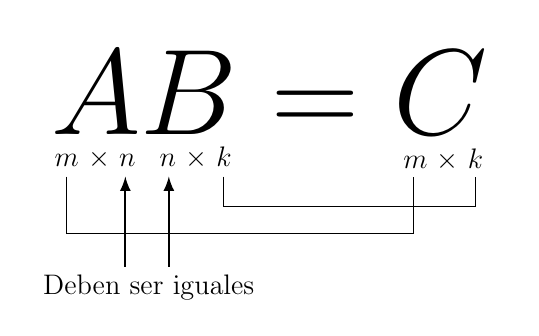
\begin{tikzpicture}[scale=0.85,transform shape]
            \begin{scope}[scale=3,transform shape]
                \node at (0,0) {\LARGE $AB = C$};
            \end{scope}
            
            \begin{scope}[xshift=-1.8cm]
                %\draw[ thick, <-,orange] (-0.15,0.25) .. controls (-0.25,0.8) and (-0.25,1.5) .. (1,1.5);
                
                %\node[right, orange] at (1,1.5) {\itshape No product symbol};
                \node[ ] at (-0.8,-1) {\large ${m}$ $\times$ $n$};
                \node[ ] at (0.7,-0.97) {\large $n$ $\times$ $k$};
                \node[ ] at (4.4,-1) {\large $m$ $\times$ $k$};
                
                \draw[thin] (1.11,-1.25)--(1.11,-1.7)--(4.88,-1.7)--(4.88,-1.25);
                \draw[thin] (-1.23,-1.25)--(-1.23,-2.1)--(3.96,-2.1)--(3.96,-1.25);
                
                \draw[thick, -latex] (-0.35,-2.6)--(-0.35,-1.25);
                \draw[thick, -latex] (0.3,-2.6)--(0.3,-1.25);
                \node at (0,-2.9) {\large Deben ser iguales};
            \end{scope}
        \end{tikzpicture}
    \end{center}
\end{observation}

\begin{example}
    En este ejemplo se muestra la forma en la cual se puede usar la multiplicación de matrices para modelar la manera en que se extiende una enfermedad contagiosa. Las enfermedades contagiosas son aquellas que se propagan de una persona a otra a través del contacto directo. Los ejemplos incluyen la gripe, el resfriado común y la COVID-19.
    
    Considere tres grupos de personas $X$, $Y$ y $Z$ con $4$, $6$ y $5$ elementos respectivamente como se muestra en la tabla \ref{tab:1}. Suponga que cuatro individuos han contraído esta enfermedad. Este grupo entra en contacto con seis personas de un segundo grupo. Estos contactos, llamados \textit{contactos directos}, se pueden representar por una matriz de $4 \times 6$. Consideremos la siguiente matriz para los grupos $X$ y $Y$:\sideTable[\label{tab:1}]{
    \centering
    \begin{tabular}{ll}
        \toprule
        \textbf{Grupo} & \textbf{Elementos} \\
        \midrule
        $X$ & $a_1$, $a_2$, $a_3$, $a_4$ \\
        $Y$ & $b_1$, $b_2$, $b_3$, $b_4$, $b_5$, $b_6$ \\
        $Z$ & $c_1$, $c_2$, $c_3$, $c_4$, $c_5$ \\
        \bottomrule
    \end{tabular}
    }
    $$A = \begin{bmatrix}
        0 & 1 & 0 & 0 & 1 & 0 \\
        1 & 0 & 0 & 1 & 0 & 1 \\
        0 & 0 & 0 & 1 & 1 & 0 \\
        1 & 0 & 0 & 0 & 0 & 1
    \end{bmatrix}$$
    En este caso se hace $a_{ij} = 1$ si la $i$-ésima persona del primer grupo entra en contacto con la $j$-ésima persona del segundo grupo. Por ejemplo, el $1$ en la posición $(2, 4)$ significa que la segunda persona del primer grupo (infectada) entró en contacto con la cuarta persona del segundo grupo. Ahora suponga que un tercer grupo de cinco personas tiene varios contactos directos con individuos del segundo grupo. Esto también se puede representar mediante una matriz.
    $$B = \begin{bmatrix}
        0 & 0 & 1 & 0 & 1 \\
        0 & 0 & 0 & 1 & 0 \\
        0 & 1 & 0 & 0 & 0 \\
        1 & 0 & 0 & 0 & 1 \\
        0 & 0 & 0 & 1 & 0 \\
        0 & 0 & 1 & 0 & 0
    \end{bmatrix}$$
    Observe que $b_{64} = 0$, lo que quiere decir que la sexta persona del segundo grupo no tiene contacto con la cuarta persona del tercer grupo.
    
    Los contactos \textit{indirectos} o de \textit{segundo orden} entre individuos del primero y tercer grupos se representan mediante la matriz de $4 \times 5$, $C = AB$. Para ver esto, observe que una persona del grupo $3$ puede quedar contagiada por alguien del grupo $2$, quien a su vez fue contagiada por alguien del grupo $1$. Por ejemplo, como $a_{24} = 1$ y $b_{45} = 1$ se ve que, indirectamente, la quinta persona del grupo $3$ tuvo contacto (a través de la cuarta persona del grupo $2$) con la segunda persona del grupo $1$. El número total de contactos indirectos entre la segunda persona del grupo $1$ y la quinta persona del grupo $3$ está dado por
    \begin{align*}
        c_{25} & = a_{21}b_{15} + a_{22}b_{25} + a_{23}b_{35} + a_{24}b_{45} + a_{25}b_{55} + a_{26}b_{65} \\
        & = 1 \cdot 1 + 0 \cdot 0 + 0 \cdot 0 + 1 \cdot 1 + 0 \cdot 0 + 1 \cdot 0 = 2
    \end{align*}
    Así pues,
    $$C = AB = \begin{bmatrix}
        0 & 0 & 0 & 2 & 0 \\
        1 & 0 & 2 & 0 & 2 \\
        1 & 0 & 0 & 1 & 1 \\
        0 & 0 & 2 & 0 & 1 
    \end{bmatrix}$$

    Observe que únicamente la segunda persona del grupo $3$ no tiene contactos indirectos con la enfermedad. La quinta persona de este grupo tiene $2 + 1 + 1 = 4$ contactos de segundo orden.
\end{example}

\begin{theorem}
    El producto de matrices es asociativo.
\end{theorem}

\begin{observation}
    El producto de matrices no es conmutativo. En efecto, sea $A$, $B \in \mathcal{M}_{2 \times 2}(\RR)$ con $A = \begin{bmatrix}
        1 & 1 \\
        0 & 1
    \end{bmatrix}$ y $B = \begin{bmatrix}
        2 & 1 \\
        1 & 1
    \end{bmatrix}$, entonces
    \begin{align*}
        AB & = \begin{bmatrix}
            1 & 1 \\
            0 & 1
        \end{bmatrix} \begin{bmatrix}
            2 & 1 \\
            1 & 1
        \end{bmatrix} \\
        & = \begin{bmatrix}
            3 & 2 \\
            1 & 1
        \end{bmatrix}
    \end{align*}
    y
    \begin{align*}
        BA & = \begin{bmatrix}
            2 & 1 \\
            1 & 1
        \end{bmatrix} \begin{bmatrix}
            1 & 1 \\
            0 & 1
        \end{bmatrix} \\
        & = \begin{bmatrix}
            2 & 3 \\
            1 & 2
        \end{bmatrix}
    \end{align*}
    Así que, en general $AB \neq BA$.
\end{observation}

\begin{notation}
    Si $A \in \mathcal{M}_{n \times n}(\RR)$ y $n \in \NN$, definimos $A^n$ como
    $$A^n = \underbrace{A A \cdots A}_{n-\text{veces}}$$
\end{notation}

\begin{definition}\label{def:matriz-idempotente}
    Sea $A \in \mathcal{M}_{n \times n}(\RR)$, decimos que $A$ es una matriz idempotente si $A^2=A$.
\end{definition}

\begin{example}
    Sea $A = \begin{bmatrix*}[r]
        -1 & 3 & 5 \\
        1 & -3 & -5 \\
        -1 & 3 & 5 \\
    \end{bmatrix*}$, entonces
    $$A^2 = \begin{bmatrix*}[r]
        -1 & 3 & 5 \\
        1 & -3 & -5 \\
        -1 & 3 & 5 \\
    \end{bmatrix*} \begin{bmatrix*}[r]
        -1 & 3 & 5 \\
        1 & -3 & -5 \\
        -1 & 3 & 5 \\
    \end{bmatrix*} = \begin{bmatrix*}[r]
        -1 & 3 & 5 \\
        1 & -3 & -5 \\
        -1 & 3 & 5 \\
    \end{bmatrix*} = A$$
    Por tanto, $A$ es idempotente.
\end{example}

\begin{definition}
    Sea $A \in \mathcal{M}_{n \times n}(\RR)$, decimos que $A$ es una matriz nilpotente si existe un entero positivo $p$ tal que $A^p=0$. El grado o índice de nilpotencia es el menor entero positivo $p$ tal que $A^p=0$.
\end{definition}

\begin{example}
    Sea $A = \begin{bmatrix*}[r]
        1 & 1 \\
        -1 & -1 \\
    \end{bmatrix*}$, entonces
    $$A^2 = \begin{bmatrix*}[r]
        1 & 1 \\
        -1 & -1 \\
    \end{bmatrix*} \begin{bmatrix*}[r]
        1 & 1 \\
        -1 & -1 \\
    \end{bmatrix*} = \begin{bmatrix*}[r]
        0 & 0 \\
        0 & 0 \\
    \end{bmatrix*}$$
    Por tanto, $A$ es nilpotente de índice de nilpotencia 2.
\end{example}

\begin{definition}
    La matriz identidad $I_n$ es una matriz de $n \times n$ cuyos elementos de la diagonal principal son iguales a $1$ y todos los demás son $0$. Esto es,
    $$I_n = \llparenthesis \delta_{ij} \rrparenthesis = \begin{cases}
        1 & \text{ si } i = j \\
        0 & \text{ si } i \neq j
    \end{cases}$$
\end{definition}

\begin{theorem}[Ley distributiva de la multiplicación de matrices]
    Si todas las sumas y todos los productos siguientes están definidos, entonces
    $$A(B + C) = AB + AC$$
    \demostracion
    Sea $A \in \mathcal{M}_{m \times p}(\RR)$ y sean $B$, $C \in \mathcal{M}_{p \times n}(\RR)$ con $A = \llparenthesis a_{ij} \rrparenthesis$, $B = \llparenthesis b_{kj} \rrparenthesis$, $C = \llparenthesis c_{kj} \rrparenthesis$. Así
    %{\small
    \begin{align*}
        A(B + C) & = \begin{bmatrix}
            a_{11} & a_{12} & \cdots & a_{1p}\\
            a_{21} & a_{22} & \cdots & a_{2p}\\
            \vdots &  & \ddots & \\
            a_{m1} & a_{m2} & \cdots & a_{mp}
        \end{bmatrix} \left( \begin{bmatrix}
            b_{11} & b_{12} & \cdots & b_{1n}\\
            b_{21} & b_{22} & \cdots & b_{2n}\\
            \vdots &  & \ddots & \\
            b_{p1} & b_{p2} & \cdots & b_{pn}
        \end{bmatrix} + \begin{bmatrix}
            c_{11} & c_{12} & \cdots & c_{1n}\\
            c_{21} & c_{22} & \cdots & c_{2n}\\
            \vdots &  & \ddots & \\
            c_{p1} & c_{p2} & \cdots & c_{pn}
        \end{bmatrix} \right) \\
        & = \begin{bmatrix}
            a_{11} & a_{12} & \cdots & a_{1p}\\
            a_{21} & a_{22} & \cdots & a_{2p}\\
            \vdots &  & \ddots & \\
            a_{m1} & a_{m2} & \cdots & a_{mp}
        \end{bmatrix} \begin{bmatrix}
            b_{11} + c_{11} & b_{12} + c_{12} & \cdots & b_{1n} + c_{1n}\\
            b_{21} + c_{21} & b_{22} + c_{22} & \cdots & b_{2n} + c_{2n}\\
            \vdots &  & \ddots & \\
            b_{p1} + c_{p1} & b_{p2} + c_{p2} & \cdots & b_{pn} + c_{pn}
        \end{bmatrix} \\
        & = \begin{bmatrix}
            \displaystyle\sum_{q=1}^{p} a_{1q}(b_{q1} + c_{q1}) & \displaystyle\sum_{q=1}^{p} a_{1q}(b_{q2} + c_{q2}) & \cdots & \displaystyle\sum_{q=1}^{p} a_{1q}(b_{qn} + c_{qn}) \\
            \displaystyle\sum_{q=1}^{p} a_{2q}(b_{q1} + c_{q1}) & \displaystyle\sum_{q=1}^{p} a_{2q}(b_{q2} + c_{q2}) & \cdots & \displaystyle\sum_{q=1}^{p} a_{2q}(b_{qn} + c_{qn}) \\
            \vdots & & \ddots & \\
            \displaystyle\sum_{q=1}^{p} a_{mq}(b_{q1} + c_{q1}) & \displaystyle\sum_{q=1}^{p} a_{mq}(b_{q2} + c_{q2}) & \cdots & \displaystyle\sum_{q=1}^{p} a_{mq}(b_{qn} + c_{qn})
        \end{bmatrix} \\
        & = \begin{bmatrix}
            \displaystyle\sum_{q=1}^{p} a_{1q}b_{q1} + \displaystyle\sum_{q=1}^{p} a_{1q}c_{q1} & \displaystyle\sum_{q=1}^{p} a_{1q}b_{q2} + \displaystyle\sum_{q=1}^{p} a_{1q}c_{q2} & \cdots & \displaystyle\sum_{q=1}^{p} a_{1q}b_{qn} + \displaystyle\sum_{q=1}^{p} a_{1q}c_{qn} \\
            \displaystyle\sum_{q=1}^{p} a_{2q}b_{q1} + \displaystyle\sum_{q=1}^{p} a_{2q}c_{q1} & \displaystyle\sum_{q=1}^{p} a_{2q}b_{q2} + \displaystyle\sum_{q=1}^{p} a_{2q}c_{q2} & \cdots & \displaystyle\sum_{q=1}^{p} a_{2q}b_{qn} + \displaystyle\sum_{q=1}^{p} a_{2q}c_{qn} \\
            \vdots & & \ddots & \\
            \displaystyle\sum_{q=1}^{p} a_{mq}b_{q1} + \displaystyle\sum_{q=1}^{p} a_{mq}c_{q1} & \displaystyle\sum_{q=1}^{p} a_{mq}b_{q2} + \displaystyle\sum_{q=1}^{p} a_{mq}c_{q2} & \cdots & \displaystyle\sum_{q=1}^{p} a_{mq}b_{qn} + \displaystyle\sum_{q=1}^{p} a_{mq}c_{qn}
        \end{bmatrix} \\
        & = \begin{bmatrix}
            \displaystyle\sum_{q=1}^{p} a_{1q}b_{q1} & \displaystyle\sum_{q=1}^{p} a_{1q}b_{q2} & \cdots & \displaystyle\sum_{q=1}^{p} a_{1q}b_{qn} \\
            \displaystyle\sum_{q=1}^{p} a_{2q}b_{q1} & \displaystyle\sum_{q=1}^{p} a_{2q}b_{q2} & \cdots & \displaystyle\sum_{q=1}^{p} a_{2q}b_{qn} \\
            \vdots & & \ddots & \\
            \displaystyle\sum_{q=1}^{p} a_{mq}b_{q1} & \displaystyle\sum_{q=1}^{p} a_{mq}b_{q2} & \cdots & \displaystyle\sum_{q=1}^{p} a_{mq}b_{qn} 
        \end{bmatrix} + \begin{bmatrix}
            \displaystyle\sum_{q=1}^{p} a_{1q}c_{q1} & \displaystyle\sum_{q=1}^{p} a_{1q}c_{q2} & \cdots & \displaystyle\sum_{q=1}^{p} a_{1q}c_{qn} \\
            \displaystyle\sum_{q=1}^{p} a_{2q}c_{q1} & \displaystyle\sum_{q=1}^{p} a_{2q}c_{q2} & \cdots & \displaystyle\sum_{q=1}^{p} a_{2q}c_{qn} \\
            \vdots & & \ddots & \\
            \displaystyle\sum_{q=1}^{p} a_{mq}c_{q1} & \displaystyle\sum_{q=1}^{p} a_{mq}c_{q2} & \cdots & \displaystyle\sum_{q=1}^{p} a_{mq}c_{qn}
        \end{bmatrix} \\
        & = AB + AC
    \end{align*}
    %}
\end{theorem}

\begin{definition}
    Sea $A \in \mathcal{M}_{n\times n} (\RR)$ y sea $f(x) \in P_n(x)$, con
    $$f(x)=a_0 + a_1 x+ \cdots +a_m x^m$$
    Definimos a $f(A)$ como:
    $$f(A)=a_0 I_n +a_1 A+\cdots +a_m A^m$$
\end{definition}

\begin{example}
    Si $f(x) = x^2 -5x +2$ y $A = \begin{bmatrix}
        2 & 0 \\
        4 & 5 \\
    \end{bmatrix}$, entonces:
    $$f(A) = \begin{bmatrix}
        2 & 0 \\
        4 & 5 \\
    \end{bmatrix} \begin{bmatrix}
        2 & 0 \\
        4 & 5 \\
    \end{bmatrix} -5 \begin{bmatrix}
        2 & 0 \\
        4 & 5 \\
    \end{bmatrix} +2 \begin{bmatrix}
        1 & 0 \\
        0 & 1 \\
    \end{bmatrix} = \begin{bmatrix*}[r]
        -4 & 0 \\
        8 & 2 \\
    \end{bmatrix*}$$
\end{example}

\begin{definition}
    Sea $A = \llparenthesis a_{ij} \rrparenthesis \in \mathcal{M}_{m \times n}(\RR)$, se define la matriz transpuesta de $A$, denotada por $A^T$ donde $A^T \in \mathcal{M}_{n \times m}(\RR)$, como sigue: Si
    $$A = \begin{bmatrix}
        a_{11} & a_{12} & \cdots & a_{1n}\\
        a_{21} & a_{22} & \cdots & a_{2n}\\
        \vdots &  & \ddots & \\
        a_{m1} & a_{m2} & \cdots & a_{mn}
    \end{bmatrix}$$
    entonces
    $$A^T = \llparenthesis a_{ji} \rrparenthesis = \begin{bmatrix}
        a_{11} & a_{21} & \cdots & a_{m1}\\
        a_{12} & a_{22} & \cdots & a_{m2}\\
        \vdots &  & \ddots & \\
        a_{1n} & a_{2n} & \cdots & a_{mn}
    \end{bmatrix}$$
\end{definition}

\begin{example}
    Un torneo de Tenis se puede organizar de la siguiente manera. Cada uno de los $n$ tenistas juega contra todas los demás y se registran los resultados en una matriz $R = \llparenthesis r_{ij} \rrparenthesis \in \mathcal{M}_{n \times n}(\RR)$ como sigue:
    $$r_{ij} = \begin{cases}
        1, & \text{ si el jugador $i$ le gana al $j$} \\
        0, & \text{ si el jugador $i$ pierde contra el $j$} \\
        0, & \text{ si $i = j$}
    \end{cases}$$
    Se asigna al tenista $i$ la calificación siguiente:
    \begin{equation}
        S_i = \sum_{j=1}^{n} r_{ij} + \frac{1}{2} \sum_{j=1}^{n} \left( R^{2} \right)_{ij} \label{ec28}
    \end{equation}
    Para un torneo de $n = 4$ tenistas, tenemos
    $$R = \begin{bmatrix}
        0 & 1 & 0 & 0 \\
        0 & 0 & 1 & 1 \\
        1 & 0 & 0 & 0 \\
        1 & 0 & 1 & 0
    \end{bmatrix} = \llparenthesis r_{ij} \rrparenthesis$$
    Para clasificar a los jugadores, primero calculemos $R^{2}$ como sigue:
    $$R^{2} = \begin{bmatrix}
        0 & 1 & 0 & 0 \\
        0 & 0 & 1 & 1 \\
        1 & 0 & 0 & 0 \\
        1 & 0 & 1 & 0
    \end{bmatrix} \begin{bmatrix}
        0 & 1 & 0 & 0 \\
        0 & 0 & 1 & 1 \\
        1 & 0 & 0 & 0 \\
        1 & 0 & 1 & 0
    \end{bmatrix} = \begin{bmatrix}
        0 & 0 & 1 & 1 \\
        2 & 0 & 1 & 0 \\
        0 & 1 & 0 & 0 \\
        1 & 1 & 0 & 0
    \end{bmatrix}$$
    Así, utilizando la ecuación \eqref{ec28}, obtenemos:
    \begin{align*}
        S_1 & = 1 + \frac{1}{2} (2) & S_2 & = 2 + \frac{1}{2} (3) & S_3 & = 1 + \frac{1}{2} (1) & S_4 & = 2 + \frac{1}{2} (2) \\
        & = 2 & & = \frac{7}{2} & & = \frac{3}{2} & & = 3
    \end{align*}
    Por tanto, $S_1 = 2$, $\displaystyle S_2 = \frac{7}{2}$, $\displaystyle S_3 = \frac{3}{2}$ y $S_4 = 4$, y además
    $$S_3 < S_1 < S_4 < S_2.$$
\end{example}

\begin{definition}
    Sea $A \in \mathcal{M}_{n \times n}(\RR)$. Si $A^T = A$, entonces decimos que la matriz $A$ es simétrica.
\end{definition}

\newpage

\begin{example}
    Sea $A = \begin{bmatrix}
        1 & 3 \\
        3 & 1
    \end{bmatrix}$. Notemos que $A^T = A$, por lo que $A$ es simétrica.
\end{example}

\begin{definition}\label{matriz-antisimetrica}
    Sea $A \in \mathcal{M}_{n \times n}(\RR)$. Si $A^T = -A$, entonces decimos que la matriz $A$ es antisimétrica.
\end{definition}

\begin{theorem}\label{theo:matrixtranspu}
    Sea $A$, $B \in \mathcal{M}_{n \times n}(\RR)$, entonces
    $$(AB)^T = B^TA^T$$
    \demostracion
    Sea
    $$A = \begin{bmatrix}
        a_{11} & a_{12} & \cdots & a_{1n}\\
        a_{21} & a_{22} & \cdots & a_{2n}\\
        \vdots &  & \ddots & \\
        a_{n1} & a_{n2} & \cdots & a_{nn}
    \end{bmatrix}$$
    entonces
    $$A^T = \begin{bmatrix}
        a_{11} & a_{21} & \cdots & a_{n1}\\
        a_{12} & a_{22} & \cdots & a_{n2}\\
        \vdots &  & \ddots & \\
        a_{1n} & a_{2n} & \cdots & a_{nn}
    \end{bmatrix}$$
    Análogamente, sea
    $$B = \begin{bmatrix}
        b_{11} & b_{12} & \cdots & b_{1n}\\
        b_{21} & b_{22} & \cdots & b_{2n}\\
        \vdots &  & \ddots & \\
        b_{n1} & b_{n2} & \cdots & b_{nn}
    \end{bmatrix}$$
    entonces
    $$B^T = \begin{bmatrix}
        b_{11} & b_{21} & \cdots & b_{n1}\\
        b_{12} & b_{22} & \cdots & b_{n2}\\
        \vdots &  & \ddots & \\
        b_{1n} & b_{2n} & \cdots & b_{nn}
    \end{bmatrix}$$
    Ahora
    $$AB = \begin{bmatrix}
        \displaystyle\sum_{q=1}^{n} a_{1q}b_{q1} & \displaystyle\sum_{q=1}^{n} a_{1q}b_{q2} & \cdots & \displaystyle\sum_{q=1}^{n} a_{1q}b_{qn} \\
        \displaystyle\sum_{q=1}^{n} a_{2q}b_{q1} & \displaystyle\sum_{q=1}^{n} a_{2q}b_{q2} & \cdots & \displaystyle\sum_{q=1}^{n} a_{2q}b_{qn} \\
        \vdots & & \ddots & \\
        \displaystyle\sum_{q=1}^{n} a_{nq}b_{q1} & \displaystyle\sum_{q=1}^{n} a_{nq}b_{q2} & \cdots & \displaystyle\sum_{q=1}^{n} a_{nq}b_{qn}
    \end{bmatrix}$$
    Por otra parte
    $$B^T A^T = \begin{bmatrix}
        \displaystyle\sum_{q=1}^{n} a_{1q}b_{q1} & \displaystyle\sum_{q=1}^{n} a_{2q}b_{q1} & \cdots & \displaystyle\sum_{q=1}^{n} a_{nq}b_{q1} \\
        \displaystyle\sum_{q=1}^{n} a_{1q}b_{q2} & \displaystyle\sum_{q=1}^{n} a_{2q}b_{q2} & \cdots & \displaystyle\sum_{q=1}^{n} a_{nq}b_{q2} \\
        \vdots & & \ddots & \\
        \displaystyle\sum_{q=1}^{n} a_{1q}b_{qn} & \displaystyle\sum_{q=1}^{n} a_{2q}b_{qn} & \cdots & \displaystyle\sum_{q=1}^{n} a_{nq}b_{qn} 
    \end{bmatrix} = (AB)^T$$
\end{theorem}

\begin{proposition}\label{propiedades_transpuesta}
    Sean $A$, $B \in \mathcal{M}_{n \times n}(\RR)$ y sea $\alpha \in \RR$, entonces
    \begin{enumerate}[label=\roman*.]
        \item $\left(A^T\right)^T = A$.
        \item $(A + B)^T = A^T + B^T$
        \item $(\alpha A)^T = \alpha A^T$
    \end{enumerate}
    \demostracion Se dejan como ejercicio al lector.
\end{proposition}

\begin{definition}
    Sea $A \in \mathcal{M}_{n \times n}(\RR)$, decimos que $A$ es una matriz diagonal si todas sus entradas fuera de la diagonal son cero, es decir, $\llparenthesis a_{ij} \rrparenthesis = 0$, para toda $i \neq j$. Si $\llparenthesis a_{ij} \rrparenthesis = a_{ij}$, entonces escribiremos $$A = \operatorname{diag} \left\lbrace a_{11}, \dots, a_{nn} \right\rbrace$$
\end{definition}

\begin{example}
    Sea
    $$A = \begin{bmatrix*}[r]
        -1 & 0 & 0 \\
        0 & -6 & 0 \\
        0 & 0 & -9 \\
    \end{bmatrix*}$$
    entonces $A = \operatorname{diag} \{ -1, -6, -9 \}$.
\end{example}

\begin{proposition}\label{propiedades_diagonal}
    Sean $A$, $B$ matrices diagonales y sea $\alpha \in \RR$, entonces
    \begin{enumerate}[label=\roman*.]
        \item $A+B$ es diagonal.
        \item $AB$ es diagonal.
        \item $\alpha A$ es diagonal.
        \item $A^{T} = A$.
    \end{enumerate}
    \demostracion Se dejan como ejercicio al lector.
\end{proposition}

\begin{definition}
    Sea $A \in \mathcal{M}_{n \times n}(\RR)$, decimos que $A$ es una matriz triangular superior si todas las entradas bajo la diagonal son cero, es decir, $\llparenthesis a_{ij} \rrparenthesis = 0$, para toda $i>j$.
\end{definition}

\begin{example}
    Un ejemplo de una matriz triangular superior es:
    \begin{center}
        \begin{tikzpicture}[
        Matrix/.style={
        matrix of nodes,
        text height=1.75ex,
        text depth=0.525ex,
        text width=2.275ex,
        align=center,
        left delimiter={[},
        right delimiter={]},
        column sep=0pt,
        row sep=0pt,
        nodes in empty cells,},
        DA/.style={
        fill=gray!20,
        dash pattern=on 3pt off 3pt,
        line width=0.7pt,
        rounded corners=5pt,}
        ]
        
        \matrix[Matrix] at (0,0) (M){
            $1$ & $6$ & $1$ \\
            $0$ & $2$ & $7$ \\
            $0$ & $0$ & $9$ \\
        };
        
        \begin{scope}[on background layer]
            \draw[DA](M-1-1.north west)
            -| (M-3-3.south east)
            -- (M-3-3.south west)
            |- (M-2-2.south west)
            |- (M-1-1.south west)
            -- cycle;
        \end{scope}
        \end{tikzpicture}
    \end{center}
\end{example}

\begin{proposition}
    Sean $A$, $B$ matrices triangulares superiores y sea $\alpha \in \RR$, entonces
    \begin{enumerate}[label=\roman*.]
        \item $A+B$ es triangular superior.
        \item $AB$ es triangular superior.
        \item $\alpha A$ es triangular superior.
    \end{enumerate}
    \demostracion Se dejan como ejercicio al lector.
\end{proposition}

\begin{definition}
    Sea $A \in \mathcal{M}_{n \times n}(\RR)$, decimos que $A$ es una matriz triangular inferior si todas las entradas sobre la diagonal son cero, es decir, $\llparenthesis a_{ij} \rrparenthesis = 0$, para toda $i<j$.
\end{definition}

\begin{example}
    Un ejemplo de una matriz triangular inferior es:
    \begin{center}
        \begin{tikzpicture}[scale=0.9,
        Matrix/.style={
        matrix of nodes,
        text height=1.75ex,
        text depth=0.525ex,
        text width=2.275ex,
        align=center,
        left delimiter={[},
        right delimiter={]},
        column sep=0pt,
        row sep=0pt,
        nodes in empty cells,},
        DA/.style={
        fill=gray!20,
        dash pattern=on 3pt off 3pt,
        line width=0.7pt,
        rounded corners=5pt,}
        ]
        
        \matrix[Matrix] at (0,0) (M1){
            $6$ & $0$ & $0$ \\
            $4$ & $3$ & $0$ \\
            $8$ & $5$ & $1$ \\
        };
        
        \begin{scope}[on background layer]
            \draw[DA](M1-1-1.north)
            -| (M1-1-1.south east)
            -| (M1-2-2.south east)
            -| (M1-3-3.south east)
            -| (M1-1-1.west)
            |- (M1-1-1.north);
        \end{scope}
        \end{tikzpicture}
    \end{center}
\end{example}

\newpage

\begin{proposition}
    Sean $A$, $B$ matrices triangulares inferiores y sea $\alpha \in \RR$, entonces
    \begin{enumerate}[label=\roman*.]
        \item $A+B$ es triangular inferior.
        \item $AB$ es triangular inferior.
        \item $\alpha A$ es triangular inferior.
    \end{enumerate}
    \demostracion Se dejan como ejercicio al lector.
\end{proposition}

\section{Sistemas de ecuaciones}

\begin{definition}\label{definicion:JSJJNDJUDUDJNDN}
    Sea $A \in \mathcal{M}_{n \times n}(\RR)$ y $\mathbb{x} \in \RR[n]$, siendo
    $$A = \begin{bmatrix}
        a_{11} & a_{12} & \cdots & a_{1n}\\
        a_{21} & a_{22} & \cdots & a_{2n}\\
        \vdots &  & \ddots & \\
        a_{m1} & a_{m2} & \cdots & a_{mn}
    \end{bmatrix} \quad \text{y} \quad \mathbb{x} = \begin{bmatrix}
        x_1 \\
        x_2 \\
        \vdots \\
        x_n
    \end{bmatrix}$$
    Se define el producto de la matriz $A$ con el vector $\mathbb{x}$ como:
    \begin{align*}
        A \mathbb{x} = \begin{bmatrix}
            a_{11} & a_{12} & \cdots & a_{1n}\\
            a_{21} & a_{22} & \cdots & a_{2n}\\
            \vdots &  & \ddots & \\
            a_{m1} & a_{m2} & \cdots & a_{mn}
        \end{bmatrix} \begin{bmatrix}
            x_1 \\
            x_2 \\
            \vdots \\
            x_n
        \end{bmatrix} = \begin{bmatrix}
            a_{11}x_1 + a_{12}x_2 + \cdots + a_{1n}x_n \\
            a_{21}x_1 + a_{22}x_2 + \cdots + a_{2n}x_n \\
            \vdots \\
            a_{m1}x_1 + a_{m2}x_2 + \cdots + a_{mn}x_n
        \end{bmatrix}
    \end{align*}
\end{definition}

\begin{definition}
    Si $A\mathbb{x} = \mathbb{b}$, obtenemos
    \begin{equation}
        \left. \begin{array}{rl}
            a_{11}x_1 + a_{12}x_2 + \cdots + a_{1n}x_n = & \!\!\!\! b_1 \\
            a_{21}x_1 + a_{22}x_2 + \cdots + a_{2n}x_n = & \!\!\!\! b_2 \\
            \vdots \hspace{1cm}  \\
            a_{m1}x_1 + a_{m2}x_2 + \cdots + a_{mn}x_n = & \!\!\!\! b_m
        \end{array} \!\!\right\} \label{ec29}
    \end{equation}
    A la expresión \eqref{ec29} se le llamará \textbf{sistema de ecuaciones lineales} (SEL) de $m$ ecuaciones con $n$ incógnitas. Además, si $\mathbb{b} = \mathbb{0}$, obtenemos
    \begin{equation*}
        \left. \begin{array}{rl}
            a_{11}x_1 + a_{12}x_2 + \cdots + a_{1n}x_n = & \!\!\!\! 0 \\
            a_{21}x_1 + a_{22}x_2 + \cdots + a_{2n}x_n = & \!\!\!\! 0 \\
            \vdots \hspace{1cm}  \\
            a_{m1}x_1 + a_{m2}x_2 + \cdots + a_{mn}x_n = & \!\!\!\! 0
        \end{array} \!\!\right\}
    \end{equation*}
    A esta expresión se le llamará sistema homogéneo.
\end{definition}

\begin{observation}
    Una solución para el sistema homogéneo es cuando $x_1 = x_2 = \cdots = x_n = 0$ y es conocida como solución trivial.
\end{observation}
\marginElement{
\begin{center}
    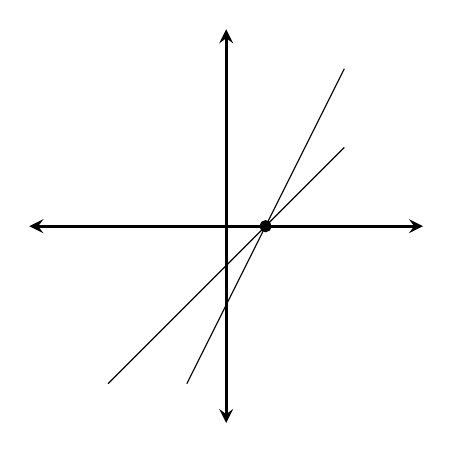
\begin{tikzpicture}
        \draw[black,stealth-stealth,very thick] (0,0) -- (5,0);
        \draw[black,stealth-stealth,very thick] (2.5,-2.5) -- (2.5,2.5);
        \draw (1,-2) -- (4,1);
        \draw (2,-2) -- (4,2);
        \filldraw (3,0) circle (2pt); 
    \end{tikzpicture}
    \textbf{i.} Sistemas con única solución
\end{center}
~\vspace{-0.5cm}
\begin{center}
    \begin{tikzpicture}
        \draw[black,stealth-stealth,very thick] (0,0) -- (5,0);
        \draw[black,stealth-stealth,very thick] (2.5,-2.5) -- (2.5,2.5);
        \draw[thick] (1,-2) -- (4,2);
        \draw (1,-2) -- (4,2);
    \end{tikzpicture}
    \textbf{ii.} Sistemas con infinitas soluciones
\end{center}
~\vspace{-0.5cm}
\begin{center}
    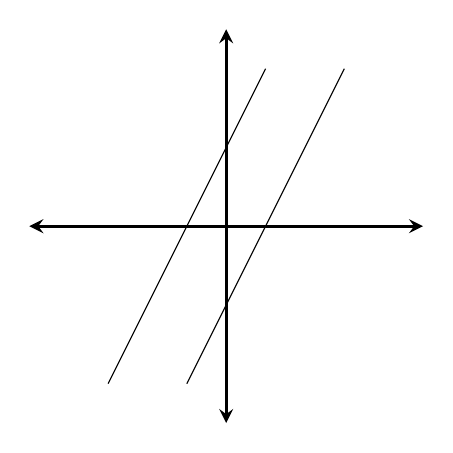
\begin{tikzpicture}
        \draw[black,stealth-stealth,very thick] (12,0) -- (17,0);
        \draw[black,stealth-stealth,very thick] (14.5,-2.5) -- (14.5,2.5);
        \draw (13,-2) -- (15,2);
        \draw (14,-2) -- (16,2);
    \end{tikzpicture}
    \textbf{iii.} Sistemas sin solución
\end{center}
\captionsetup*[figure]{font={footnotesize},hypcap=false}%
\captionof{figure}{Representación de los posibles casos del conjunto solución de un SEL $2 \times 2$}\label{JWISIKSJSKISOOKKOOOOIUKKSK}
}

Consideremos el siguiente sistema de dos ecuaciones lineales con dos incógnitas $x_1$, $x_2$:
$$\left. \begin{array}{rl}
    a_{11}x_1+a_{12}x_2 = & \!\!\!\! b_1 \\ 
    a_{21}x_1+a_{22}x_2 = & \!\!\!\! b_2 \\
\end{array} \!\!\right\}$$
donde $a_{11}$, $a_{12}$, $a_{21}$, $a_{22}$, $b_1$, $b_2$ son números dados. Notemos que cada una de estas ecuaciones corresponde a una recta. Cualquier par ordenado de números reales $(x_1, x_2)$ que satisface dicho sistema se denomina como solución. Notemos que en este sistema existen tres posibles casos: cuando existe una única solución, infinitas soluciones o el conjunto solución es el vacío. Vea la figura \ref{JWISIKSJSKISOOKKOOOOIUKKSK}.
\newpage
\marginElement{
\begin{center}
    \tdplotsetmaincoords{70}{110}
    \begin{tikzpicture}[tdplot_main_coords,scale=0.65]
        \begin{scope}
            \draw[fill=gray!50,opacity=0.3] (0,0,0) -- (0,-3,-1) -- (0,-3,-3) -- (0,0,-3) -- cycle;
            \draw[fill=gray!60,opacity=0.3] (-3,-3,-1) -- (-3,0,0) -- (3,0,0) -- (3,-3,-1) -- cycle;
            \draw[fill=gray!50,opacity=0.3] (0,-3,3) -- (0,0,3) -- (0,0,0) -- (0,-3,-1) -- cycle;
            \draw[fill=gray!80,opacity=0.4] (-3,0,-3) -- (-3,0,3) -- (3,0,3) -- (3,0,-3) -- cycle;
            \draw[fill=gray!50,opacity=0.3] (0,0,0) -- (0,3,1) -- (0,3,-3) -- (0,0,-3) -- cycle;
            \draw[fill=gray!60,opacity=0.3] (-3,0,0) -- (-3,3,1) -- (3,3,1) -- (3,0,0) -- cycle;
            \draw[fill=gray!50,opacity=0.3] (0,0,0) -- (0,0,3) -- (0,3,3) -- (0,3,1) -- cycle;
            \filldraw (0,0,0) circle(4pt);
        \end{scope}
    \end{tikzpicture}
    \\ \textbf{i.} Sistemas con única solución
\end{center}
~\vspace{-0.5cm}
\begin{center}
    \tdplotsetmaincoords{70}{110}
    \begin{tikzpicture}[tdplot_main_coords,scale=0.65]
        \begin{scope}[xshift=8cm]
            \draw[fill=gray!50,opacity=0.3] (-3,0,0) -- (-3,-1,-3) -- (3,-1,-3) -- (3,0,0) -- cycle;
            \draw[fill=gray!60,opacity=0.3] (-3,-3,-1) -- (-3,0,0) -- (3,0,0) -- (3,-3,-1) -- cycle;
            \draw[fill=gray!80,opacity=0.4] (-3,0,-3) -- (-3,0,3) -- (3,0,3) -- (3,0,-3) -- cycle;
            \draw[fill=gray!60,opacity=0.3] (-3,0,0) -- (-3,3,1) -- (3,3,1) -- (3,0,0) -- cycle;
            \draw[fill=gray!50,opacity=0.3] (-3,1,3) -- (-3,0,0) -- (3,0,0) -- (3,1,3) -- cycle;
            \draw[thick, dashed, black](-3,0,0)--(3,0,0); 
        \end{scope}
    \end{tikzpicture}
    \\ \textbf{ii.} Sistemas con infinitas soluciones
\end{center}
~\vspace{-0.5cm}
\begin{center}
    \tdplotsetmaincoords{70}{110}
    \begin{tikzpicture}[tdplot_main_coords,scale=0.65]
        \draw[dash pattern=on 3pt off 3pt] (-3,-3,0) -- (-3,-3,5);
        \draw[fill=gray!50,opacity=0.3] (-3,-3,0) -- (-3,3,0) -- (3,3,0) -- (3,-3,0) -- cycle;
        \draw[fill=gray!70,opacity=0.35] (-3,-3,2.5) -- (-3,3,2.5) -- (3,3,2.5) -- (3,-3,2.5) -- cycle;
        \draw[fill=gray!90,opacity=0.4] (-3,-3,5) -- (-3,3,5) -- (3,3,5) -- (3,-3,5) -- cycle;
        \draw[dash pattern=on 3pt off 3pt] (-3,3,0) -- (-3,3,5);
        \draw[dash pattern=on 3pt off 3pt] (3,3,0) -- (3,3,5);
        \draw[dash pattern=on 3pt off 3pt] (3,-3,0) -- (3,-3,5);
    \end{tikzpicture}
    \,\\
    \tdplotsetmaincoords{80}{93}
    \begin{tikzpicture}[tdplot_main_coords,scale=0.8]
        \begin{scope}[xshift=16cm]
            \draw[fill=gray!50,opacity=0.3] (-3,-1,2) -- (-3,2,-2) -- (3,2,-2) -- (3,-1,2) -- cycle;
            \draw[fill=gray!80,opacity=0.4] (-3,1,2) -- (-3,-2,-2) -- (3,-2,-2) -- (3,1,2) -- cycle;
            \draw[fill=gray!60,opacity=0.3] (-3,-3,-1)--(-3,3,-1)--(3,3,-1)--(3,-3,-1) -- cycle;
            \draw[dashed,thick](-3,-1.25,-1)--(3,-1.25,-1);
            \draw[dashed,thick](-3,1.25,-1)--(3,1.25,-1);
            \draw[dashed,thick](-2.7,0,0.75)--(3,0,0.75);
            \draw[thin](-3,-1.25,-1)--(3,-1.25,-1);
            \draw[thin](-3,1.25,-1)--(3,1.25,-1);
            \draw[thin](-2.7,0,0.75)--(3,0,0.75);
        \end{scope}
    \end{tikzpicture}
    \\ \textbf{iii.} Sistemas sin solución
\end{center}
\captionsetup*[figure]{font={footnotesize},hypcap=false}%
\captionof{figure}{Representación de los posibles casos del conjunto solución de un SEL $3 \times 3$}\label{KSKJSJSJJJJSJSJJSDDDD}
}

Ahora, consideremos el siguiente sistema de tres ecuaciones lineales con tres incógnitas $x_1$, $x_2$, $x_3$:
$$\left. \begin{array}{rl}
    a_{11}x_1+a_{12}x_2+a_{13}x_3 = & \!\!\!\! b_1 \\ 
    a_{21}x_1+a_{22}x_2+a_{23}x_3 = & \!\!\!\! b_2 \\ 
    a_{31}x_1+a_{32}x_2+a_{33}x_3 = & \!\!\!\! b_3
\end{array} \!\!\right\}$$
donde $a_{11}$, $a_{12}$, $a_{13}$, $a_{21}$, $a_{22}$, $a_{23}$, $a_{31}$, $a_{32}$, $a_{33}$, $b_1$, $b_2$, $b_3$ son números dados. Notemos que cada una de estas ecuaciones corresponde a un plano. Cualquier terna de números reales $(x_1, x_2, x_3)$ que satisface dicho sistema se denomina como solución. De manera análoga respecto al SEL $2 \times 2$ anterior, en este sistema existen tres posibles casos: cuando existe una única solución, infinitas soluciones o el conjunto solución es el vacío. Es difícil dibujar con exactitud los planos en distintos casos, pero se pueden reducir como se muestra en la figura \ref{KSKJSJSJJJJSJSJJSDDDD}.

\begin{observation}
    Observemos que en la definición \ref{definicion:JSJJNDJUDUDJNDN} se puso a $\mathbb{x}$ como una matriz de tamaño $n \times 1$, cuando al principio de dicha definición se dijo que pertenecía a $\RR[n]$. Aunque pueda parecer un error, no es así, pues $\mathbb{x}$ se puede representar de ambas maneras, sea como vector o como matriz de tamaño $n \times 1$. Así que si $\mathbb{x} \in \RR[n]$, entonces $\mathbb{x} \in \mathcal{M}_{n \times 1}(\RR)$. Cuando consideremos a $\mathbb{x} \in \mathcal{M}_{n \times 1}(\RR)$, escribiremos a $\mathbb{x}$ como:
    $$\mathbb{x} = \begin{bmatrix}
        x_1 \\
        x_2 \\
        \vdots \\
        x_n
    \end{bmatrix}$$
    en vez de
    $$\mathbb{x} = \begin{pmatrix}
        x_1 \\
        x_2 \\
        \vdots \\
        x_n
    \end{pmatrix}$$
    Esto nos será de gran ayuda para entender de mejor manera los sistemas de ecuaciones lineales y no confundirnos con la notación.
\end{observation}

\section{Núcleo e imagen de una matriz}

\begin{definition}
    Sea $A \in \matrizmn$, se define el espacio nulo de $A$, denotado por $\mathcal{N}_A$, como:
    $$\mathcal{N}_A = \left\{ \mathbb{x} \in \RR[n] \mid A\mathbb{x} = \mathbb{0} \in \RR[m] \right\}$$
    Al espacio nulo de $A$ también de le llama kernel de $A$, o bien, núcleo de $A$.
\end{definition}

\begin{proposition}
    $\mathcal{N}_A$ es un subespacio de $\RR[n]$. \\
    \demostracion Basta probar que $\mathcal{N}_A$ cumple (i) y (ii) del teorema \ref{theorem:JAJSUJGBUHBOSOIOOSK}. Así pues:
    \begin{enumerate}[label=\roman*)]
        \item Sean $\mathbb{x}$, $\mathbb{y} \in \mathcal{N}_A$, entonces
        \begin{equation*}
            A\mathbb{x} = \mathbb{0} \quad \text{y} \quad A\mathbb{y} = \mathbb{0} \label{ec30}
        \end{equation*}
        Ahora
        \begin{align*}
            A(\mathbb{x}+\mathbb{y}) & = A \mathbb{x} + A \mathbb{y} \\
            & = \mathbb{0} + \mathbb{0} = \mathbb{0}
        \end{align*}
        Entonces $\mathbb{x} + \mathbb{y} \in \mathcal{N}_A$. Por tanto, se cumple la propiedad de cerradura para la suma.\newpage
        \item Sea $\alpha \in \RR$, veamos que $\alpha \mathbb{x} \in \mathcal{N}_A$. Así
        \begin{align*}
            A(\alpha \cdot \mathbb{x}) & = \begin{bmatrix}
                a_{11} & a_{12} & \cdots & a_{1n}\\
                a_{21} & a_{22} & \cdots & a_{2n}\\
                \vdots &  & \ddots & \\
                a_{m1} & a_{m2} & \cdots & a_{mn}
            \end{bmatrix} \begin{bmatrix}
                \alpha x_1 \\
                \alpha x_2 \\
                \vdots \\
                \alpha x_n
            \end{bmatrix} \\
            & = \begin{bmatrix}
                a_{11}\alpha x_1 + a_{12}\alpha x_2 + \cdots + a_{1n}\alpha x_n \\
                a_{21}\alpha x_1 + a_{22}\alpha x_2 + \cdots + a_{2n}\alpha x_n \\
                \vdots \\
                a_{m1}\alpha x_1 + a_{m2}\alpha x_2 + \cdots + a_{mn}\alpha x_n
            \end{bmatrix} \\
            & = \begin{bmatrix}
                \alpha \left( a_{11}x_1 + a_{12}x_2 + \cdots + a_{1n}x_n \right) \\
                \alpha \left( a_{21}x_1 + a_{22}x_2 + \cdots + a_{2n}x_n \right) \\
                \vdots \\
                \alpha \left( a_{m1}x_1 + a_{m2}x_2 + \cdots + a_{mn}x_n \right)
            \end{bmatrix} \\
            & = \alpha A \mathbb{x} \\
            & = \alpha \cdot \mathbb{0} = \mathbb{0}
        \end{align*}
        Entonces $\alpha \mathbb{x} \in \mathcal{N}_A$. Por tanto, se cumple la propiedad de cerradura para la multiplicación de un escalar por un vector.
    \end{enumerate}
    De (i) y (ii), se sigue que $\mathcal{N}_A$ es subespacio de $\RR[n]$.
\end{proposition}

\begin{definition}
    Llamaremos nulidad de $A$, denotada por $\nu(A)$, a la $\Dim(\mathcal{N}_A)$, es decir
    $$\nu(A) = \Dim(\mathcal{N}_A)$$
\end{definition}

\begin{example}
    Sea $A = \begin{bmatrix*}[r]
        1 & 2 & -1 \\
        2 & -1 & 3
    \end{bmatrix*} \in \mathcal{M}_{2 \times 3}(\RR)$, determine $\mathcal{N}_A$. \\
    \solucion Por definición,
    \begin{align*}
        \mathcal{N}_A & = \left\{ \mathbb{x} \in \RR[3] \mid A\mathbb{x} = \mathbb{0} \right\} \\
        & = \left\{ \begin{pmatrix}
            x_1 \\
            x_2 \\
            x_3
        \end{pmatrix} \mid \begin{bmatrix*}[r]
            1 & 2 & -1 \\
            2 & -1 & 3
        \end{bmatrix*} \begin{bmatrix}
            x_1 \\
            x_2 \\
            x_3
        \end{bmatrix} = \begin{bmatrix}
            0 \\
            0
        \end{bmatrix} \right\} \\
        & = \left\{ \begin{pmatrix}
            x_1 \\
            x_2 \\
            x_3
        \end{pmatrix} \mid \begin{bmatrix}
            x_1 + 2x_2 - x_3 \\
            2x_1 - x_2 + 3x_3
        \end{bmatrix} = \begin{bmatrix}
            0 \\
            0
        \end{bmatrix} \right\}
    \end{align*}
    Entonces
    $$\left. \begin{array}{r}
        x_1 + 2x_2 - x_3 = 0\\
        2x_1 - x_2 + 3x_3 = 0
    \end{array} \right\}$$
    Multiplicando la segunda ecuación por $2$, obtenemos
    $$\left. \begin{array}{r}
        x_1 + 2x_2 - x_3 = 0\\
        4x_1 - 2x_2 + 6x_3 = 0
    \end{array} \right\}$$
    Sumando la primer ecuación con la segunda, obtenemos
    $$5x_1 + 5x_3 = 0$$
    Por tanto, $x_3 = -x_1$. Sustituyendo en la primer ecuación, obtenemos
    $$2x_1 + 2x_2 = 0$$
    Por tanto, $x_2 = -x_1$. Se sigue entonces
    \begin{align*}
        \mathcal{N}_A & = \left\{ \begin{pmatrix*}[r]
            x_1 \\
            -x_1 \\
            -x_1
        \end{pmatrix*} \mid x_1 \in \RR \right\} \\
        & = \left\{ x_1 \cdot \begin{pmatrix*}[r]
            1 \\
            -1 \\
            -1
        \end{pmatrix*} \mid x_1 \in \RR \right\} \\
        & = \Gen \left( \left\{ \begin{pmatrix*}[r]
            1 \\
            -1 \\
            -1
        \end{pmatrix*} \right\} \right)
    \end{align*}
    Por tanto, $\mathcal{N}_A = \Gen \left( \left\{ \begin{pmatrix*}[r]
        1 \\
        -1 \\
        -1
    \end{pmatrix*} \right\} \right)$.  Además, $\nu(A) = 1$.
\end{example}

\begin{example}
    Dada $A = \begin{bmatrix*}[r]
        1 & 2 \\
        1 & -1
    \end{bmatrix*}$. Determine $\mathcal{N}_A$ y $\nu(A)$. \\
    \solucion Por definición,
    \begin{align*}
        \mathcal{N}_A & = \left\{ \mathbb{x} \in \RR[2] \mid A\mathbb{x} = \mathbb{0} \in \RR[2] \right\} \\
        & = \left\{ \begin{pmatrix}
            x_1 \\
            x_2
        \end{pmatrix} \in \RR[2] \mid \begin{bmatrix*}[r]
            1 & 2 \\
            1 & -1
        \end{bmatrix*} \begin{bmatrix}
            x_1 \\
            x_2
        \end{bmatrix} = \begin{bmatrix}
            0 \\
            0
        \end{bmatrix} \right\} \\
        & = \left\{ \begin{pmatrix}
            x_1 \\
            x_2
        \end{pmatrix} \in \RR[2] \mid \begin{bmatrix}
            x_1 + 2x_2 \\
            x_1 - x_2
        \end{bmatrix} = \begin{bmatrix}
            0 \\
            0
        \end{bmatrix} \right\}
    \end{align*}
    Entonces
    $$\left. \begin{array}{r}
        x_1 + 2x_2 = 0\\
        x_1 - x_2 = 0
    \end{array} \right\}$$
    Restando la primer ecuación de la segunda, obtenemos que
    $$3x_2 = 0 \Longrightarrow x_2 = 0$$
    y sustituyendo en la segunda ecuación se obtiene que
    $$x_1 = 0$$
    Se sigue entonces que
    $$x_1 = 0 \quad \text{y} \quad x_2 = 0$$
    por lo que
    \begin{align*}
        \mathcal{N}_A & = \left( \left\{ \begin{pmatrix}
            0 \\
            0
        \end{pmatrix} \right\} \right) \\
        & = \Gen \left( \left\{ \begin{pmatrix}
            0 \\
            0
        \end{pmatrix} \right\} \right)
    \end{align*}
    Por tanto, $\mathcal{N}_A = \Gen \left( \left\{ \begin{pmatrix}
        0 \\
        0
    \end{pmatrix} \right\} \right)$.  Además, $\nu(A) = 0$.
\end{example}

\begin{remark}
    Recordemos que la dimensión de un espacio vectorial se define como la cantidad de vectores linealmente independientes necesarios para generar todo el espacio. En el caso del vector cero, su dimensión es $0$ porque no puede generar ningún otro vector aparte de sí mismo mediante combinaciones lineales. Para entenderlo mejor, considera que cualquier vector $\mathbb{v}$ en un espacio vectorial $V$ puede ser expresado como:
    $$\mathbb{v} = c_1 \mathbb{v}_1 + c_2 \mathbb{v}_2 + \cdots + c_n \mathbb{v}_n$$
    donde $\mathbb{v}_1, \mathbb{v}_2, \dots, \mathbb{v}_n$ son vectores l.i en $V$, y $c_1, c_2, \dots, c_n$ son escalares.
    
    Ahora, si consideramos el vector cero $\mathbb{0}$, no importa cuánto intentemos expresarlo como una combinación lineal de otros vectores $\mathbb{v}_1, \mathbb{v}_2, \dots, \mathbb{v}_n$, siempre obtendremos $\mathbb{0}$ como resultado, ya que cualquier escalar multiplicado por $\mathbb{0}$ sigue siendo $\mathbb{0}$.
    
    Por lo tanto, la dimensión del espacio generado por el vector cero es igual a $0$, ya que no requiere ningún otro vector para ser generado, y no puede generar ningún otro vector aparte de sí mismo.
\end{remark}

\begin{definition}
    Sea $A \in \matrizmn$, se define la imagen de la matriz $A$, denotado por $\Ima(A)$, como
    $$\Ima(A) = \left\{ \mathbb{y} \in \RR[m] \mid A\mathbb{x} = \mathbb{y}, \text{ para algún } \mathbb{x} \in \RR[n] \right\}$$
\end{definition}

\begin{theorem}
    Sea $A \in \matrizmn$, entonces $\Ima(A) \subseteq \RR[2]$ es un subespacio.\\
    \demostracion
    \begin{enumerate}[label=\roman*)]
        \item Sean $\mathbb{y}_1$, $\mathbb{y}_2 \in \Ima(A)$, entonces
        \begin{equation}
            A\mathbb{x}_1 = \mathbb{y}_1, \text{ para algún } \mathbb{x}_1 \in \RR[n] \label{UYHDFHDFVFDVFVHFD}
        \end{equation}
        y
        \begin{equation}
            A\mathbb{x}_2 = \mathbb{y}_2, \text{ para algún } \mathbb{x}_2 \in \RR[n] \label{HFHDVJHFHJUGHHFGJ}
        \end{equation}
        Así
        \begin{align*}
            \mathbb{y}_1 + \mathbb{y}_2 & = A\mathbb{x}_1 + A\mathbb{x}_2 && \text{al sustituir \eqref{UYHDFHDFVFDVFVHFD} y \eqref{HFHDVJHFHJUGHHFGJ}} \\
            & = A(\mathbb{x}_1 + \mathbb{x}_2) && \text{por distributividad} \\
            & = A\mathbb{w} && \text{siendo $\mathbb{w} = \mathbb{x}_1 + \mathbb{x}_2$}
        \end{align*}
        esto es $\mathbb{y}_1 + \mathbb{y}_2 = A\mathbb{w}$, para algún $\mathbb{w} \in \RR[n]$. Por tanto, $\mathbb{y}_1 + \mathbb{y}_2 \in \Ima(A)$, es decir, se cumple la cerradura bajo la suma.
        \item Se deja como ejercicio al lector.
    \end{enumerate}
    Así, se verifica que $\Ima(A)$ es un subespacio.
\end{theorem}

\begin{definition}
    Sea $A \in \matrizmn$. Se llama rango de la matriz $A$, denotado por $\rho(A)$, como
    $$\rho(A) = \Dim\big(\Ima(A)\big)$$
\end{definition}

\begin{example}
    Dada la matriz
    $$A = \begin{bmatrix*}[r]
        1 & 2 \\
        1 & -1
    \end{bmatrix*},$$
    determine $\Ima(A)$ y $\rho(A)$. \\
    \solucion Por definición,
    \begin{align*}
        \Ima(A) & = \left\{ \mathbb{y} \in \RR[2] \mid A\mathbb{x} = \mathbb{y}, \text{ para algún } \mathbb{x} \in \RR[2] \right\} \\
        & = \left\{ \begin{pmatrix}
            y_1 \\
            y_2
        \end{pmatrix} \in \RR[2] \mid \begin{bmatrix*}[r]
            1 & 2 \\
            1 & -1
        \end{bmatrix*} \begin{bmatrix}
            x_1 \\
            x_2
        \end{bmatrix} = \begin{bmatrix}
            y_1 \\
            y_2
        \end{bmatrix}, \text{ para algún } \mathbb{x} \in \RR[2] \right\} \\
        & = \left\{ \begin{pmatrix}
            y_1 \\
            y_2
        \end{pmatrix} \in \RR[2] \mid \begin{bmatrix}
            x_1 + 2x_2 \\
            x_1 - x_2
        \end{bmatrix} = \begin{bmatrix}
            y_1 \\
            y_2
        \end{bmatrix}, \text{ para algún } \mathbb{x} \in \RR[2] \right\} \\
        & = \left\{ \begin{pmatrix}
            y_1 \\
            y_2
        \end{pmatrix} \in \RR[2] \mid x_1 \begin{pmatrix}
            1 \\
            1
        \end{pmatrix} + x_2 \begin{pmatrix*}[r]
            2 \\
            -1
        \end{pmatrix*} = \begin{pmatrix}
            y_1 \\
            y_2
        \end{pmatrix}, \text{ para algún } \mathbb{x} \in \RR[2] \right\} \\
        & = \left\{ x_1 \begin{pmatrix}
            1 \\
            1
        \end{pmatrix} + x_2 \begin{pmatrix*}[r]
            2 \\
            -1
        \end{pmatrix*}, \; x_1, x_2 \in \RR \right\} \\
        & = \Gen \left(\left\{ \begin{pmatrix}
            1 \\
            1
        \end{pmatrix},  \begin{pmatrix*}[r]
            2 \\
            -1
        \end{pmatrix*} \right\}\right)
    \end{align*}
    Observemos que el conjunto de vectores
    $$\left\{ \begin{pmatrix}
            1 \\
            1
        \end{pmatrix},  \begin{pmatrix*}[r]
            2 \\
            -1
        \end{pmatrix*} \right\}$$
    es l.i. Por tanto, $\Ima(A) = \Gen \left(\left\{ \begin{pmatrix}
        1 \\
        1
    \end{pmatrix},  \begin{pmatrix*}[r]
        2 \\
        -1
    \end{pmatrix*} \right\}\right)$ y $\rho(A) = 2$.
\end{example}

\begin{example}\label{HSGDGFDHFYTGGGGGFBVH}
    Dada la matriz
    $$B = \begin{bmatrix*}[r]
        1 & -1 & 2 & 3 \\
        0 & 1 & 4 & 3 \\
        1 & 0 & 6 & 6
    \end{bmatrix*},$$
    determine $\mathcal{N}_B$, $\Ima(B)$, $\nu(B)$ y $\rho(B)$. \\
    \solucion Por definición,
    \begin{align*}
        \mathcal{N}_B & = \left\{ \mathbb{x} \in \RR[4] \mid B\mathbb{x} = \mathbb{0} \in \RR[3] \right\} \\
        & = \left\{ \begin{pmatrix}
            x_1 \\
            x_2 \\
            x_3 \\
            x_4
        \end{pmatrix} \in \RR[4] \mid \begin{bmatrix*}
            1 & -1 & 2 & 3 \\
            0 & 1 & 4 & 3 \\
            1 & 0 & 6 & 6
        \end{bmatrix*} \begin{bmatrix}
            x_1 \\
            x_2 \\
            x_3 \\
            x_4
        \end{bmatrix} = \begin{bmatrix}
            0 \\
            0 \\
            0
        \end{bmatrix} \right\} \\
        & = \left\{ \begin{pmatrix}
            x_1 \\
            x_2 \\
            x_3 \\
            x_4
        \end{pmatrix} \in \RR[4] \mid \begin{bmatrix}
            x_1 - x_2 + 2x_3 + 3x_4 \\
            x_2 + 4x_3 + 3x_4 \\
            x_1 + 6x_3 + 6x_4
        \end{bmatrix} = \begin{bmatrix}
            0 \\
            0 \\
            0
        \end{bmatrix} \right\}
    \end{align*}
    Entonces
    \begin{align}
        x_1 - x_2 + 2x_3 + 3x_4 & = 0 \label{JHFJHJFHKJVHFDJLK} \\
        x_2 + 4x_3 + 3x_4 & = 0 \label{HDHFJDFHDJH} \\
        x_1 + 6x_3 + 6x_4 & = 0 \label{NHDFJVNDJBJJVDBFJHRJK}
    \end{align}
    Notemos que, sumando \eqref{JHFJHJFHKJVHFDJLK} y \eqref{HDHFJDFHDJH}, se obtiene \eqref{NHDFJVNDJBJJVDBFJHRJK}. De \eqref{NHDFJVNDJBJJVDBFJHRJK}, se obtiene que
    $$x_1 = -6x_3 - 6x_4,  x_2 \in \RR$$
    Se sigue pues
    \begin{align*}
        \mathcal{N}_B & = \left\{ \begin{pmatrix}
            -6x_3 - 6x_4 \\
            0 \\
            x_3 \\
            x_4
        \end{pmatrix} \right\} \\
        & = \left\{ x_3 \begin{pmatrix*}[r]
            -6\\
            0 \\
            1 \\
            0
        \end{pmatrix*} + x_4 \begin{pmatrix*}[r]
            -6 \\
            0 \\
            0 \\
            1
        \end{pmatrix*}, \; \text{ con } x_3,  x_4 \in \RR \right\} \\
        & = \Gen \left(\left\{ \begin{pmatrix*}[r]
            -6 \\
            0 \\
            1 \\
            0
        \end{pmatrix*},  \begin{pmatrix*}[r]
            -6 \\
            0 \\
            0 \\
            1
        \end{pmatrix*} \right\}\right)
    \end{align*}
    Observemos que el conjunto de vectores
    $$\left\{ \begin{pmatrix*}[r]
        -6 \\
        0 \\
        1 \\
        0
    \end{pmatrix*},  \begin{pmatrix*}[r]
        -6 \\
        0 \\
        0 \\
        1
    \end{pmatrix*} \right\}$$\newpage\noindent
    es l.i. Por tanto, $\mathcal{N}_B = \Gen \left(\left\{ \begin{pmatrix*}[r]
        -6 \\
        0 \\
        1 \\
        0
    \end{pmatrix*},  \begin{pmatrix*}[r]
        -6 \\
        0 \\
        0 \\
        1
    \end{pmatrix*} \right\}\right)$ y $\nu(B) = 2$. Ahora, por definición,
    \begin{align*}
        \Ima(B) & = \left\{ \mathbb{y} \in \RR[3] \mid A\mathbb{x} = \mathbb{y}, \text{ para algún } \mathbb{x} \in \RR[4] \right\} \\
        & = \left\{ \begin{pmatrix}
            y_1 \\
            y_2 \\
            y_3
        \end{pmatrix} \in \RR[3] \mid \begin{bmatrix*}[r]
            1 & -1 & 2 & 3 \\
            0 & 1 & 4 & 3 \\
            1 & 0 & 6 & 6
        \end{bmatrix*} \begin{bmatrix}
            x_1 \\
            x_2 \\
            x_3
        \end{bmatrix} = \begin{bmatrix}
            y_1 \\
            y_2 \\
            y_3
        \end{bmatrix}, \text{ para algún } \mathbb{x} \in \RR[4] \right\} \\
        & = \left\{ \begin{pmatrix}
            y_1 \\
            y_2 \\
            y_3
        \end{pmatrix} \in \RR[3] \mid \begin{bmatrix}
            x_1 - x_2 + 2x_3 + x_4 \\
            x_2 + 4x_3 + 3x_4 \\
            x_1 + 6x_2 + 6x_4
        \end{bmatrix} = \begin{bmatrix}
            y_1 \\
            y_2 \\
            y_3
        \end{bmatrix}, \text{ para algún } \mathbb{x} \in \RR[4] \right\} \\
        & = \left\{ \begin{pmatrix}
            y_1 \\
            y_2 \\
            y_3
        \end{pmatrix} \in \RR[3] \mid x_1 \begin{pmatrix}
            1 \\
            0 \\
            1
        \end{pmatrix} + x_2 \begin{pmatrix*}[r]
            -1 \\
            1 \\
            0
        \end{pmatrix*} + x_3 \begin{pmatrix}
            2 \\
            4 \\
            6
        \end{pmatrix} + x_4 \begin{pmatrix}
            3 \\
            3 \\
            6
        \end{pmatrix}, \; x_1,  x_2,  x_3,  x_4 \in \RR \right\} \\
        & = \Gen \left(\left\{ \begin{pmatrix}
            1 \\
            0 \\
            1
        \end{pmatrix},  \begin{pmatrix*}[r]
            -1 \\
            1 \\
            0
        \end{pmatrix*},  \begin{pmatrix}
            2 \\
            4 \\
            6
        \end{pmatrix},  \begin{pmatrix}
            3 \\
            3 \\
            6
        \end{pmatrix} \right\}\right) \\
        & = \Gen \left(\left\{ \begin{pmatrix}
            1 \\
            0 \\
            1
        \end{pmatrix},  \begin{pmatrix*}[r]
            -1 \\
            1 \\
            0
        \end{pmatrix*} \right\}\right)
    \end{align*}
    Por tanto, $\Ima(B) = \Gen \left(\left\{ \begin{pmatrix}
        1 \\
        0 \\
        1
    \end{pmatrix},  \begin{pmatrix*}[r]
        -1 \\
        1 \\
        0
    \end{pmatrix*} \right\}\right)$ y $\rho(B) = 2$.
\end{example}

\begin{definition}
    Sea $A \in \matrizmn$ y sean $\REN[A] = \left\{ \mathbb{r}_1,  \mathbb{r}_2,  \dots,  \mathbb{r}_m \right\}$ el conjunto de renglones de la matriz $A$ y $\COL[A] = \left\{ \mathbb{c}_1,  \mathbb{c}_2,  \dots,  \mathbb{c}_n \right\}$ el conjunto de columnas de la matriz $A$. Esto es
    \begin{equation*}  
        A=
        \begin{tikzpicture}[baseline=(m-3-1.base)]
            \matrix [matrix of math nodes,left delimiter=(,right delimiter=),row sep=0.05cm,column sep=0.05cm] (m) {
            a_{11} & a_{12} & \dots  & a_{1j} & \dots & a_{1n}\\
            a_{21} & a_{22} & \dots  & a_{2j} & \dots & a_{2n}\\  
            \vdots & \vdots &  & \vdots  &  & \vdots\\
            a_{i1} & a_{i2} & \dots  & a_{ij} & \dots & a_{in}\\
            \vdots & \vdots &  & \vdots  &  & \vdots\\
            a_{m1} & a_{m2} & \dots  & a_{mj} & \dots & a_{mn}\\};

            \begin{scope}[nodes={text width=1.1em,align=center}]
                \node[above=10pt of m-1-1] (top-1) {$\mathbb{c}_1$};
                \node[above=10pt of m-1-2] (top-2) {$\mathbb{c}_2$};
                \node[above=14pt of m-1-3] (top-3) {$\cdots$};
                \node[above=9pt of m-1-4] (top-4) {$\mathbb{c}_j$};
                \node[above=14pt of m-1-5] (top-5) {$\cdots$};
                \node[above=10pt of m-1-6] (top-6) {$\mathbb{c}_n$};
            \end{scope}

            \node[right=13pt of m-1-6] (left-1) {$\mathbb{r}_1$};
            \node[right=13pt of m-2-6] (left-1) {$\mathbb{r}_1$};
            \node[right=16pt of m-3-6] (left-1) {$\quad\!\!\vdots$};
            \node[right=15pt of m-4-6] (left-1) {$\mathbb{r}_i$};
            \node[right=16pt of m-5-6] (left-1) {$\quad\!\!\vdots$};
            \node[right=13pt of m-6-6] (left-1) {$\mathbb{r}_m$};
        \end{tikzpicture}
    \end{equation*}
    Definimos el espacio de renglones de $A$, denotado por $\mathcal{R}_A$, como
    $$\mathcal{R}_A = \Gen \left( \left\{ \mathbb{r}_1, \mathbb{r}_2, \dots, \mathbb{r}_m \right\} \right) \subseteq \RR[n]$$
    y el espacio de vectores columna, denotado por $\mathcal{C}_A$, como
    $$\mathcal{C}_A = \Gen \left( \left\{ \mathbb{c}_1, \mathbb{c}_2, \dots, \mathbb{c}_n \right\} \right) \subseteq \RR[m]$$
\end{definition}

\begin{example}
    Tomando la matriz del ejemplo anterior, tenemos pues
    $$\REN[B] = \left\{ \mathbb{r}_1 = \begin{pmatrix*}[r]
        1 \\
        -1 \\
        2 \\
        3
    \end{pmatrix*},  \mathbb{r}_2 = \begin{pmatrix*}[r]
        0 \\
        1 \\
        4 \\
        3
    \end{pmatrix*}, \mathbb{r}_1 = \begin{pmatrix*}[r]
        1 \\
        0 \\
        6 \\
        6
    \end{pmatrix*} \right\}$$
    y
    $$\COL[B] = \left\{ \mathbb{c}_1 = \begin{pmatrix*}[r]
        1 \\
        0 \\
        1
    \end{pmatrix*},  \mathbb{c}_2 = \begin{pmatrix*}[r]
        -1 \\
        1 \\
        0
    \end{pmatrix*}, \mathbb{c}_3 = \begin{pmatrix*}[r]
        2 \\
        4 \\
        6 
    \end{pmatrix*},  \mathbb{c}_4 = \begin{pmatrix*}[r]
        3 \\
        3 \\
        6 
    \end{pmatrix*} \right\}$$\newpage\noindent
    Así
    $$\mathcal{C}_B = \Gen \left(\left\{ \begin{pmatrix}
        1 \\
        0 \\
        1
    \end{pmatrix},  \begin{pmatrix*}[r]
        -1 \\
        1 \\
        0
    \end{pmatrix*} \right\}\right) \quad \text{ y } \quad \mathcal{R}_B = \Gen \left(\left\{ \begin{pmatrix}
        0 \\
        1 \\
        4 \\
        3
    \end{pmatrix},  \begin{pmatrix*}[r]
        1 \\
        0 \\
        6 \\
        6
    \end{pmatrix*} \right\}\right)$$
    Además, observemos que $\Dim(\mathcal{R}_B) = 2$ y $\Dim(\mathcal{C}_B) = 2$.
\end{example}

\begin{theorem}
    Sea $A \in \matrizmn$, entonces
    $$\Dim(\mathcal{C}_A) = \Dim(\mathcal{R}_A) = \rho(A) = \Dim\big( \Ima(A) \big)$$
\end{theorem}

\begin{example}
    Sea $A \in \mathcal{M}_{3 \times 3}(\RR)$, dada por
    $$A = \begin{bmatrix*}[r]
        1 & -1 & 3 \\
        2 & 0 & 4 \\
        -1 & 3 & 1
    \end{bmatrix*}.$$
    Por definición:
    \begin{align*}
        \mathcal{N}_A & = \left\{ \begin{pmatrix}
            x_1 \\
            x_2 \\
            x_3 
        \end{pmatrix} \in \RR[3] \mid \begin{bmatrix*}
            1 & -1 & 3 \\
            2 & 0 & 4 \\
            -1 & 3 & 1
        \end{bmatrix*} \begin{bmatrix}
            x_1 \\
            x_2 \\
            x_3
        \end{bmatrix} = \begin{bmatrix}
            0 \\
            0 \\
            0
        \end{bmatrix} \right\} \\
        & = \left\{ \begin{pmatrix}
            x_1 \\
            x_2 \\
            x_3 \\
        \end{pmatrix} \in \RR[3] \mid \begin{bmatrix}
            x_1 - x_2 + 3x_3 \\
            2x_1 + 4x_3 \\
            -x_1 + 3x_2 + x_3
        \end{bmatrix} = \begin{bmatrix}
            0 \\
            0 \\
            0
        \end{bmatrix} \right\}
    \end{align*}
    entonces
    \begin{align}
        x_1 - x_2 + 3x_3 & = 0 \label{JDHFJDJKDHJVHFHGHKH} \\
        2x_1 + 4x_3 & = 0 \label{FHGHGFIUFHUGIHUFIHGUITY} \\
        -x_1 + 3x_2 + x_3 & = 0 \label{FHHGJHGHGUITHYTIUHYTI}
    \end{align}
    Sumando \eqref{JDHFJDJKDHJVHFHGHKH} con \eqref{FHHGJHGHGUITHYTIUHYTI}, obtenemos
    $$ +
    {
    \extrarowheight = -0.5ex
    \renewcommand{\arraystretch}{2}
    \begin{array}{rl}
        x_1 - x_2 + 3x_3= & \!\!\!\! 0 \\
        -x_1 + 3x_2 + x_3= & \!\!\!\! 0 \\
        \hline
        0x_1 + 2x_2 + 4x_3= & \!\!\!\! 0
    \end{array}}
    $$
    Multiplicando por $-2$ la ecuación \eqref{JDHFJDJKDHJVHFHGHKH} y sumándola con \eqref{FHGHGFIUFHUGIHUFIHGUITY}, se sigue que
    $$ +
    {
    \extrarowheight = -0.5ex
    \renewcommand{\arraystretch}{2}
    \begin{array}{rl}
        -2x_1 + 2x_2 - 6x_3= & \!\!\!\! 0 \\
        2x_1 + 4x_3= & \!\!\!\! 0 \\
        \hline
        0x_1 + 2x_2 - 2x_3= & \!\!\!\! 0
    \end{array}}
    $$
    Si se restan las ecuaciones obtenidas anteriormente, se sigue que
    $$ -
    {
    \extrarowheight = -0.5ex
    \renewcommand{\arraystretch}{2}
    \begin{array}{rl}
        0x_1 + 2x_2 + 4x_3= & \!\!\!\! 0 \\
        0x_1 + 2x_2 - 2x_3= & \!\!\!\! 0 \\
        \hline
        0x_1 + 0x_2 + 6x_3= & \!\!\!\! 0
    \end{array}}
    $$
    Por tanto, $x_3 = 0$. Sustituyendo hacia atrás, se obtiene que $x_2 = 0$ y $x_1 = 0$. Es decir,
    $$x_1 = 0, \quad x_2 = 0, \quad x_3 = 0$$\newpage\noindent
    Luego, $\mathcal{N}_A = \left\{ \begin{pmatrix}
        0 \\
        0 \\
        0
    \end{pmatrix} \right\}$ y $\nu(A) = 0$. Ahora, por definición,
    \begin{align*}
        \Ima(A) & = \left\{ \begin{pmatrix}
            y_1 \\
            y_2 \\
            y_3
        \end{pmatrix} \in \RR[3] \mid \begin{bmatrix*}[r]
            1 & -1 & 3 \\
            2 & 0 & 4 \\
            -1 & 3 & 1
        \end{bmatrix*} \begin{bmatrix}
            x_1 \\
            x_2 \\
            x_3
        \end{bmatrix} = \begin{bmatrix}
            y_1 \\
            y_2 \\
            y_3
        \end{bmatrix}, \text{ para algún } \mathbb{x} \in \RR[3] \right\} \\
        & = \left\{ \begin{pmatrix}
            y_1 \\
            y_2 \\
            y_3
        \end{pmatrix} \in \RR[3] \mid \begin{bmatrix}
            x_1 - x_2 + 3x_3 \\
            2x_1 + 4x_3 \\
            -x_1 + 3x_2 + x_3
        \end{bmatrix} = \begin{bmatrix}
            y_1 \\
            y_2 \\
            y_3
        \end{bmatrix}, \text{ para algún } \mathbb{x} \in \RR[3] \right\} \\
        & = \left\{ \begin{pmatrix}
            y_1 \\
            y_2 \\
            y_3
        \end{pmatrix} \in \RR[3] \mid x_1 \begin{pmatrix*}[r]
            1 \\
            2 \\
            -1
        \end{pmatrix*} + x_2 \begin{pmatrix*}[r]
            -1 \\
            0 \\
            3
        \end{pmatrix*} + x_3 \begin{pmatrix}
            3 \\
            4 \\
            1
        \end{pmatrix}, \; x_1,  x_2,  x_3 \in \RR \right\} \\
        & = \left\{ x_1 \begin{pmatrix*}[r]
            1 \\
            2 \\
            -1
        \end{pmatrix*} + x_2 \begin{pmatrix*}[r]
            -1 \\
            0 \\
            3
        \end{pmatrix*} + x_3 \begin{pmatrix}
            3 \\
            4 \\
            1
        \end{pmatrix}, \; x_1,  x_2,  x_3 \in \RR \right\} \\
        & = \Gen \left(\left\{ \begin{pmatrix*}[r]
            1 \\
            2 \\
            -1
        \end{pmatrix*},  \begin{pmatrix*}[r]
            -1 \\
            0 \\
            3
        \end{pmatrix*},  \begin{pmatrix}
            3 \\
            4 \\
            1
        \end{pmatrix} \right\}\right)
    \end{align*}
    Veamos si
    $$\begin{pmatrix}
        3 \\
        4 \\
        1
    \end{pmatrix} = a \begin{pmatrix*}[r]
        1 \\
        2 \\
        -1
    \end{pmatrix*} + b \begin{pmatrix*}[r]
        -1 \\
        0 \\
        3
    \end{pmatrix*}$$
    entonces
    \begin{align}
        a - b & = 3 \label{HFHFHUIUTHUTHRUITUJHUG} \\
        2a & = 4 \label{FDGHGFHFGUTHGHTHUITHGTJHITJITH} \\
        -a + 3b & = 1 \label{HDFRHYGUGGRTGRGTRGGHRFGHRGHHU}
    \end{align}
    De \eqref{FDGHGFHFGUTHGHTHUITHGTJHITJITH} se obtiene que $a = 2$. Sustituyendo en \eqref{HFHFHUIUTHUTHRUITUJHUG}, se obtiene que $b=-1$. Finalmente, sustituyendo en \eqref{HDFRHYGUGGRTGRGTRGGHRFGHRGHHU}, se obtiene que
    $$-2 + 3(-1) = 1$$
    lo cual no es cierto. Por lo tanto, no existen $a$, $b \in \RR$ tales que se cumpla \eqref{HDFRHYGUGGRTGRGTRGGHRFGHRGHHU}. Por tanto, el conjunto
    $$\left\{ \begin{pmatrix*}[r]
        1 \\
        2 \\
        -1
    \end{pmatrix*},  \begin{pmatrix*}[r]
        -1 \\
        0 \\
        3
    \end{pmatrix*},  \begin{pmatrix}
        3 \\
        4 \\
        1
    \end{pmatrix} \right\}$$
    es l.i. Finalmente, $\Ima(A) = \Gen \left(\left\{ \begin{pmatrix*}[r]
        1 \\
        2 \\
        -1
    \end{pmatrix*},  \begin{pmatrix*}[r]
        -1 \\
        0 \\
        3
    \end{pmatrix*},  \begin{pmatrix}
        3 \\
        4 \\
        1
    \end{pmatrix} \right\}\right)$ y $\rho(A) = 3$. Por el teorema anterior
    $$\Dim(\mathcal{C}_A) = \Dim(\mathcal{R}_A) = \rho(A) = 3$$
\end{example}

\section{Matrices invertibles}

\begin{definition}
    Sea $A \in \mathcal{M}_{n \times n}(\RR)$. Si existe $B \in \mathcal{M}_{n \times n}(\RR)$ tal que
    $$AB = BA = I$$
    entonces diremos que $B$ es la matriz inversa de $A$, y se denota por $B = A^{-1}$, es decir,
    $$AA^{-1} = A^{-1}A = I$$
    \begin{enumerate}[label=\roman*)]
        \item Si existe $A^{-1}$, diremos que $A$ es invertible o no singular.
        \item Si no existe la inversa de $A$, diremos que $A$ es no invertible o singular.
    \end{enumerate}
\end{definition}

\newpage

\begin{theorem}
    Sea $A \in \mathcal{M}_{n \times n}(\RR)$ una matriz invertible, entonces la inversa de $A$ es única. \\
    \demostracion Como $A$ es una matriz invertible, entonces existe una matriz $A^{-1} \in \mathcal{M}_{n \times n}(\RR)$ tal que
    $$AA^{-1} = A^{-1}A = I$$
    Supongamos que
    $$AM = MA = I$$
    para alguna matriz $M \in \mathcal{M}_{n \times n}(\RR)$. Así
    \begin{align*}
        M & = MI \\
        & = M(AA^{-1}) \\
        & = (MA) A^{-1} \\
        & = IA^{-1} \\
        & = A^{-1}
    \end{align*}
    Entonces $M = A^{-1}$ y por lo tanto, la inversa de $A$ es única.
\end{theorem}

\begin{theorem}
    Sean $A$, $B \in \mathcal{M}_{n \times n}(\RR)$ dos matrices invertibles, entonces $AB$ es invertible y
    $$(AB)^{-1} = B^{-1}A^{-1}$$
    \demostracion Como $A$ y $B$ son matrices invertibles, entonces existe la matriz inversa de $A$, es decir, existe $A^{-1} \in \mathcal{M}_{n \times n}(\RR)$ tal que
    $$AA^{-1} = A^{-1}A = I$$
    y de manera análoga, existe $B^{-1} \in \mathcal{M}_{n \times n}(\RR)$ tal que
    $$BB^{-1} = B^{-1}B = I$$
    Luego
    \begin{align*}
        (AB)(B^{-1}A^{-1}) & = A(BB^{-1})A^{-1} \\
        & = AIA^{-1} \\
        & = AA^{-1} \\
        & = I
    \end{align*}
    Entonces $(AB)(B^{-1}A^{-1}) = I$. Así que $(AB)^{-1} = B^{-1}A^{-1}$.
\end{theorem}

Consideremos el sistema
\begin{align*}
    a_{11}x_1 + a_{12}x_2 + \cdots + a_{1n}x_n &= b_1 \\
    a_{21}x_1 + a_{22}x_2 + \cdots + a_{2n}x_n &= b_2 \\
    &\vdots \\
    a_{m1}x_1 + a_{m2}x_2 + \cdots + a_{mn}x_n &= b_n
\end{align*}
Sea \( A \) la matriz de coeficientes del sistema, es decir
\[
    A = \begin{bmatrix}
        a_{11} & a_{12} & \cdots & a_{1n}\\
        a_{21} & a_{22} & \cdots & a_{2n}\\
        \vdots &  & \ddots & \\
        a_{m1} & a_{m2} & \cdots & a_{mn}
    \end{bmatrix}
\] \newpage\noindent
Si \( \mathbb{x} = \begin{bmatrix} x_1 \\ x_2 \\ \vdots \\ x_n \end{bmatrix} \) y \( \mathbb{b} = \begin{bmatrix} b_1 \\ b_2 \\ \vdots \\ b_n \end{bmatrix} \), entonces el sistema anterior puede ser representado matricialmente como
\[
    A\mathbb{x} = \begin{bmatrix}
        a_{11} & a_{12} & \cdots & a_{1n}\\
        a_{21} & a_{22} & \cdots & a_{2n}\\
        \vdots &  & \ddots & \\
        a_{m1} & a_{m2} & \cdots & a_{mn}
    \end{bmatrix}
    \begin{bmatrix}
        x_1 \\
        x_2 \\
        \vdots \\
        x_n
    \end{bmatrix}
    =
    \begin{bmatrix}
        a_{11}x_1 & a_{12}x_2 & \cdots & a_{1n}x_n \\
        a_{21}x_1 & a_{22}x_2 & \cdots & a_{2n}x_n \\
        \vdots &  & \ddots & \\
        a_{m1}x_1 & a_{m2}x_2 & \cdots & a_{mn}x_n
    \end{bmatrix}
    =
    \begin{bmatrix}
        b_1 \\
        b_2 \\
        \vdots \\
        b_n
    \end{bmatrix}
    = \mathbb{b}
\]
es decir,
\begin{equation}
    A\mathbb{x} = \mathbb{b} \label{DHFHGHKFHGJTHUGHTGTHIGHTUHGUTHGHJU}
\end{equation}
De \eqref{DHFHGHKFHGJTHUGHTGTHIGHTUHGUTHGHJU}, si $A$ es invertible, entonces existe $A^{-1}$. Ahora, de \eqref{DHFHGHKFHGJTHUGHTGTHIGHTUHGUTHGHJU}
\begin{align*}
    A^{-1}(A\mathbb{x}) & = A^{-1}(\mathbb{b}) \\
    (A^{-1}A)\mathbb{x} & = A^{-1}(\mathbb{b}) \\
    I\mathbb{x} & = A^{-1}(\mathbb{b})
\end{align*}
Por tanto,
$$\mathbb{x} = A^{-1}\mathbb{b}$$
que corresponde a la solución del sistema de ecuaciones.

\section{Operaciones elementales en los renglones de una matriz}

Las operaciones elementales en los renglones de una matriz son un conjunto de tres operaciones básicas que se pueden aplicar a los renglones de una matriz sin cambiar su solución. Estas operaciones son fundamentales en la resolución de sistemas de ecuaciones lineales y en la obtención de formas escalonadas o reducidas por filas de una matriz. Cada una de estas operaciones tiene un propósito específico en la manipulación de sistemas de ecuaciones lineales y en la simplificación de cálculos posteriores.

\begin{tcolorbox}[
        theorem style=change break,
        enhanced,
        breakable,
        boxrule=0pt,
        frame hidden,
        %borderline west={3pt}{0pt}{gray_50},
        colback=gray!20,
        coltitle=gray,
        attach title to upper={\ },
        sharp corners,
        fonttitle=\bfseries,
        fontupper=\normalsize,
    ]
    Dada una matriz $A$, las operaciones elementales por renglones son:
    \begin{itemize}
        \item \textbf{Intercambiar dos renglones.} Si intercambiamos los renglones $i$ y $j$, escribiremos
        \[ \mathbb{r}_i \rightleftarrows \mathbb{r}_j \]
        \item \textbf{Multiplicar un renglón por una constante no cero.} Si multiplicamos el renglón $i$ por la constante no cero $\alpha$, escribiremos
        \[ \mathbb{r}_i \leftarrow \alpha\mathbb{r}_i \]
        \item \textbf{Sumarle a un renglón un múltiplo de otro renglón.} Si le sumamos al renglón $i$, $\alpha$-veces el renglón $j$, escribiremos
        \[ \mathbb{r}_i \leftarrow \mathbb{r}_i + \alpha\mathbb{r}_j \]
    \end{itemize}
\end{tcolorbox}

La determinación de la inversa de una matriz es esencial en álgebra lineal y tiene aplicaciones fundamentales en diversos campos. Un método efectivo para encontrar la inversa de una matriz es utilizar la matriz aumentada
$$[A \mid I]$$
y aplicar las operaciones elementales antes mencionadas para que la matriz de la izquierda se convierte en la identidad, mientras que la matriz de la derecha sea la inversa deseada.

\begin{example}\label{GVSDVGVGVFGVGFGVGVGVDODSOPDKODSOKDSOKDSOP}
    Sea $A = \begin{bmatrix*}[r]
        0 & 2 & 3 \\
        2 & -6 & 8 \\
        1 & -2 & 5
    \end{bmatrix*}$. La matriz aumentada de $A$ es
    $$[A \mid I]$$
    mediante operaciones elementales, encontremos la inversa de $A$ como sigue:
    \begin{align*}
        & \left[ \begin{array}{rrr|rrr}
            0 & 2 & 3 & 1 & 0 & 0 \\
            2 & -6 & 8 & 0 & 1 & 0 \\
            1 & -2 & 5 & 0 & 0 & 1
        \end{array} \right] \xrightarrow{\mathbb{r}_1 \rightleftarrows \mathbb{r}_3} \left[ \begin{array}{rrr|rrr}
            1 & -2 & 5 & 0 & 0 & 1 \\
            2 & -6 & 8 & 0 & 1 & 0 \\
            0 & 2 & 3 & 1 & 0 & 0
        \end{array} \right] \\
        & \xrightarrow{\mathbb{r}_2 \leftarrow \mathbb{r}_2 + (-2) \mathbb{r}_1} \left[ \begin{array}{rrr|rrr}
            1 & -2 & 5 & 0 & 0 & 1 \\
            0 & -2 & -2 & 0 & 1 & -2 \\
            0 & 2 & 3 & 1 & 0 & 0
        \end{array} \right] \xrightarrow{\mathbb{r}_2 \leftarrow (-\frac{1}{2}) \mathbb{r}_2} \left[ \begin{array}{rrr|rrr}
            1 & -2 & 5 & 0 & 0 & 1 \\
            0 & 1 & 1 & 0 & -1/2 & 1 \\
            0 & 2 & 3 & 1 & 0 & 0
        \end{array} \right] \\
        & \xrightarrow{\mathbb{r}_3 \leftarrow \mathbb{r}_3 + (-2) \mathbb{r}_2} \left[ \begin{array}{rrr|rrr}
            1 & -2 & 5 & 0 & 0 & 1 \\
            0 & 1 & 1 & 0 & -1/2 & 1 \\
            0 & 0 & 1 & 1 & 1 & -2
        \end{array} \right] \xrightarrow{\mathbb{r}_1 \leftarrow \mathbb{r}_1 + (2) \mathbb{r}_2} \left[ \begin{array}{rrr|rrr}
            1 & 0 & 7 & 0 & -1 & 3 \\
            0 & 1 & 1 & 0 & -1/2 & 1 \\
            0 & 0 & 1 & 1 & 1 & -2
        \end{array} \right] \\
        & \xrightarrow{\mathbb{r}_2 \leftarrow \mathbb{r}_2 + (-1)\mathbb{r}_3} \left[ \begin{array}{rrr|rrr}
            1 & 0 & 7 & 0 & -1 & 3 \\
            0 & 1 & 0 & -1 & -3/2 & 3 \\
            0 & 0 & 1 & 1 & 1 & -2
        \end{array} \right]  \xrightarrow{\mathbb{r}_1 \leftarrow \mathbb{r}_1 + (-7) \mathbb{r}_3} \left[ \begin{array}{rrr|rrr}
            1 & 0 & 0 & -7 & -8 & 17 \\
            0 & 1 & 0 & -1 & -3/2 & 3 \\
            0 & 0 & 1 & 1 & 1 & -2
        \end{array} \right]
    \end{align*}
    Veamos que
    $$\begin{bmatrix*}[r]
        0 & 2 & 3 \\
        2 & -6 & 8 \\
        1 & -2 & 5
    \end{bmatrix*} \begin{bmatrix*}[r]
        -7 & -8 & 17 \\
        -1 & -3/2 & 3 \\
        1 & 1 & -2
    \end{bmatrix*} = \begin{bmatrix}
        1 & 0 & 0 \\
        0 & 1 & 1 \\
        0 & 0 & 1
    \end{bmatrix}$$
    Por tanto,
    $$A^{-1} = \begin{bmatrix*}[r]
        -7 & -8 & 17 \\
        -1 & -3/2 & 3 \\
        1 & 1 & -2
    \end{bmatrix*}$$
\end{example}

Con este método, se pueden resolver un sistema de ecuaciones. Vea el siguiente ejemplo. 

\begin{example}
    Sea el sistema
    \begin{equation}
        \left. \begin{array}{rl}
            2x_1+x_2= & \!\!\!\! 1 \\
            x_1+2x_2= & \!\!\!\! 2
        \end{array} \right\} \label{ISJDJUSJSJKZJKOSOPOSO}
    \end{equation}
    Empleando el método de la matriz aumentada:
    \begin{enumerate}
        \item El sistema se expresa como un sistema matricial
        $$A\mathbb{x}=\mathbb{b}$$
        Esto es
        $$\begin{bmatrix}
            2 & 1 \\
            1 & 2
        \end{bmatrix} \begin{bmatrix}
            x_1 \\
            x_2
        \end{bmatrix} = \begin{bmatrix}
            1 \\
            2
        \end{bmatrix}$$
        con $A = \begin{bmatrix}
            2 & 1 \\
            1 & 2
        \end{bmatrix}$, $\mathbb{x} = \begin{bmatrix}
            x_1 \\
            x_2
        \end{bmatrix}$, $\mathbb{b} = \begin{bmatrix}
            1 \\
            2
        \end{bmatrix}$.
        \item La matriz aumentada de $A$ es
        $$[A \mid \mathbb{b}] = \left[ \begin{array}{cc|c}
            2 & 1 & 1 \\
            1 & 2 & 2
        \end{array} \right]$$
        \item Se aplica el procedimiento anterior a la matriz aumentada. Así
        \begin{align*}
            & \left[ \begin{array}{cc|c}
                2 & 1 & 1 \\
                1 & 2 & 2
            \end{array} \right] \xrightarrow{\mathbb{r}_1 \rightleftarrows \mathbb{r}_2} \left[ \begin{array}{cc|c}
                1 & 2 & 2 \\
                2 & 1 & 1
            \end{array} \right] \xrightarrow{\mathbb{r}_2 \leftarrow \mathbb{r}_2 + (-2) \mathbb{r}_1} \left[ \begin{array}{rr|r}
                1 & 2 & 2 \\
                0 & -3 & -3
            \end{array} \right] \\
            & \xrightarrow{\mathbb{r}_2 \leftarrow (-\frac{1}{3})\mathbb{r}_2} \left[ \begin{array}{rr|r}
                1 & 2 & 2 \\
                0 & 1 & 1
            \end{array} \right] \xrightarrow{\mathbb{r}_1 \leftarrow \mathbb{r}_1 + (-2) \mathbb{r}_2} \left[ \begin{array}{rr|r}
                1 & 0 & 0 \\
                0 & 1 & 1
            \end{array} \right]
        \end{align*}
        Se obtiene un sistema equivalente
        $$\begin{bmatrix}
            1 & 0 \\
            0 & 1
        \end{bmatrix} \begin{bmatrix}
            x_1 \\
            x_2
        \end{bmatrix} = \begin{bmatrix}
            0 \\
            1
        \end{bmatrix}$$
        entonces
        $$\begin{bmatrix}
            x_1+0x_2 \\
            0x_1+x_2
        \end{bmatrix} = \begin{bmatrix}
            0 \\
            1
        \end{bmatrix}$$
        es decir,
        \begin{align*}
            x_1+0x_2 & = 0 \\
            0x_1+x_2 & = 1
        \end{align*}
        por lo que $x_1 = 0$ y $x_2 = 1$.
    \end{enumerate}
\end{example}

\begin{remark}
    Al método para resolver un sistema de ecuaciones lineales se le llamara método de Gauss-Jordan.
\end{remark}

\begin{proposition}
    Dada $A \in \mathcal{M}_{n \times n}(\RR)$ invertible, entonces
    $$\left(A^{-1}\right)^{-1} = A$$
    \demostracion Como $A$ es invertible, entonces existe $A^{-1} \in \mathcal{M}_{n \times n}(\RR)$ tal que
    $$AA^{-1}=I$$
    Sea $W = A^{-1}$, esto es $AW=I$. Además, $A$ es la matriz inversa de $W$, esto es
    \begin{equation}
        W = A^{-1} \label{KAJSJSJKSKSJNBNNKK}
    \end{equation}
    y $W$ es la matriz inversa de $A$. Es decir,
    \begin{equation}
        A = W^{-1} \label{IOSOPPPKSKSKLS}
    \end{equation}
    Sustituyendo \eqref{KAJSJSJKSKSJNBNNKK} en \eqref{IOSOPPPKSKSKLS},
    \begin{align*}
        A & = W^{-1} \\
        & = \left(A^{-1}\right)^{-1}
    \end{align*}
    Por tanto, $\left(A^{-1}\right)^{-1} = A$.
\end{proposition}

\begin{example}
    En el ejemplo \ref{HSGDGFDHFYTGGGGGFBVH}, llegamos al siguiente sistema
    \begin{align*}
        x_1 - x_2 + 2x_3 + 3x_4 & = 0 \\
        x_2 + 4x_3 + 3x_4 & = 0 \\
        x_1 + 6x_3 + 6x_4 & = 0 
    \end{align*}
    Aplicando el método de Gauss-Jordan al sistema anterior. Consideremos la matriz aumentada
    $$[A \mid \mathbb{0}]$$
    Así
    \begin{align*}
        & \left[\begin{array}{rrrr|r}
            1 & -1 & 2 & 3 & 0 \\
            0 & 1 & 4 & 3 & 0 \\
            1 & 0 & 6 & 6 & 0
        \end{array}\right] \xrightarrow{\mathbb{r}_3 \leftarrow \mathbb{r}_3 + (-1) \mathbb{r}_1} \left[\begin{array}{rrrr|r}
            1 & -1 & 2 & 3 & 0 \\
            0 & 1 & 4 & 3 & 0 \\
            0 & 1 & 4 & 3 & 0
        \end{array}\right] \\
        & \xrightarrow{\mathbb{r}_3 \leftarrow \mathbb{r}_3 + (-1) \mathbb{r}_2} \left[\begin{array}{rrrr|r}
            1 & -1 & 2 & 3 & 0 \\
            0 & 1 & 4 & 3 & 0 \\
            0 & 0 & 0 & 0 & 0
        \end{array}\right] \xrightarrow{\mathbb{r}_1 \leftarrow \mathbb{r}_1 + (1) \mathbb{r}_2} \left[\begin{array}{rrrr|r}
            1 & 0 & 6 & 6 & 0 \\
            0 & 1 & 4 & 3 & 0 \\
            0 & 0 & 0 & 0 & 0
        \end{array}\right]
    \end{align*}
    donde se obtiene el sistema equivalente dado por
    \begin{align*}
        x_1 + 6x_3 + 6x_4 & = 0 \\
        x_2 + 4x_3 + 3x_4 & = 0
    \end{align*}
    Entonces
    \begin{align*}
        x_1 & = -6x_3 - 6x_4 \\
        x_2 & = -4x_3 - 3x_4
    \end{align*}
    Así
    \begin{align*}
        \mathcal{N}_B & = \left\{ \begin{pmatrix}
            -6x_3 - 6x_4 \\
            -4x_3 - 3x_4 \\
            x_3 \\
            x_4
        \end{pmatrix} \mid x_3,  x_4 \in \RR \right\} \\
        & = \left\{ x_3 \begin{pmatrix*}[r]
            -6 \\
            -4 \\
            1 \\
            0
        \end{pmatrix*} + x_4 \begin{pmatrix*}[r]
            -6 \\
            -3 \\
            0 \\
            1
        \end{pmatrix*} \mid x_3,  x_4 \in \RR \right\} \\
        & = \Gen \left(\left\{ \begin{pmatrix*}[r]
            -6 \\
            -4 \\
            1 \\
            0
        \end{pmatrix*},  \begin{pmatrix*}[r]
            -6 \\
            -3 \\
            0 \\
            1
        \end{pmatrix*} \right\}\right)
    \end{align*}
    y además son l.i. Por tanto, $\left\{ \begin{pmatrix*}[r]
        -6 \\
        -4 \\
        1 \\
        0
    \end{pmatrix*},  \begin{pmatrix*}[r]
        -6 \\
        -3 \\
        0 \\
        1
    \end{pmatrix*} \right\}$ es una base de $\mathcal{N}_A$.
\end{example}

\begin{example}
    Resolver el siguiente sistema por el método de Gauss-Jordan
    \begin{align*}
        x+8y-5z &=3\\
        3x-2y+3z &=1\\
        2x+3y-z &=4
    \end{align*}
    \solucion Aplicando operaciones elementales a la matriz aumentada de $A$, se sigue que
    \begin{align*}
        & [A \mid \mathbb{b}] = \left[ \begin{array}{rrr|r}
            1 & 8 & -5 & 3\\
            3 & -2 & 3 & 1 \\
            2 & 3 & -1 & 4
        \end{array} \right] \xrightarrow{\mathbb{r}_2 \leftarrow \mathbb{r}_2 -3\mathbb{r}_1} \left[ \begin{array}{rrr|r}
            1 & 8 & -5 & 3\\
            0 & -26 & 18 & -8 \\
            2 & 3 & -1 & 4
        \end{array} \right] \\
        & \xrightarrow{\mathbb{r}_3 \leftarrow \mathbb{r}_3 -2\mathbb{r}_1} \left[ \begin{array}{rrr|r}
            1 & 8 & -5 & 3\\
            0 & -26 & 18 & -8 \\
            0 & -13 & 9 & 2
        \end{array} \right] \xrightarrow{\mathbb{r}_3 \rightleftarrows \mathbb{r}_2} \left[ \begin{array}{rrr|r}
            1 & 8 & -5 & 3\\
            0 & -13 & 9 & 2 \\
            0 & -26 & 18 & -8
        \end{array} \right] \\
        & \xrightarrow{\mathbb{r}_3 \leftarrow \mathbb{r}_3 -2\mathbb{r}_2} \left[ \begin{array}{rrr|r}
            1 & 8 & -5 & 3 \\
            0 & -13 & 9 & 2 \\
            0 & 0 & 0 & -4
        \end{array} \right]
    \end{align*}
    Nótese que obtenemos un sistema equivalente:
    \begin{align*}
        x+8y-5z & = 3\\
        -13y+9z & = -2\\
        0 & = -4
    \end{align*}
    Por lo que el sistema no tiene solución.
\end{example}

\begin{example}
    Resuelva el siguiente sistema:
    \begin{align*}
        2x_2 + 3x_3 & = 8 \\
        2x_1 - 6x_2 + 8x_3 & = 2 \\
        x_1 - 2x_2 + 5x_3 & = 7
    \end{align*}\newpage
    \solucion Este sistema se puede escribir en su forma matricial, es decir,
    $$A \mathbb{x} = \mathbb{b}$$
    donde
    $$A = \begin{bmatrix*}[r]
        0 & 2 & 3 \\
        2 & -6 & 8 \\
        1 & -2 & 5
    \end{bmatrix*} \quad \text{ y } \quad \mathbb{b} = \begin{bmatrix}
        8 \\
        2 \\
        7
    \end{bmatrix}$$
    Observemos que la matriz $A$ es invertible y que además
    $$A^{-1} = \begin{bmatrix*}[r]
        -7 & -8 & 17 \\
        -1 & -3/2 & 3 \\
        1 & 1 & -2
    \end{bmatrix*}$$
    por el ejemplo \ref{GVSDVGVGVFGVGFGVGVGVDODSOPDKODSOKDSOKDSOP}. Así, la única solución está dada por
    $$\mathbb{x} = A^{-1}\mathbb{b} = \begin{bmatrix*}[r]
        -7 & -8 & 17 \\
        -1 & -3/2 & 3 \\
        1 & 1 & -2
    \end{bmatrix*} \begin{bmatrix}
        8 \\
        2 \\
        7
    \end{bmatrix} = \begin{bmatrix*}[r]
        47 \\
        10 \\
        -4
    \end{bmatrix*}$$
\end{example}

\begin{theorem}
    Sea $A \in \matrizmn$, entonces
    $$\Dim(\mathcal{N}_A) + \Dim\big( \Ima(A) \big) = n$$
    siendo $m \leq n$, o bien
    $$\nu(A) + \rho(A) = n$$
\end{theorem}

\begin{example}
    En el ejemplo \ref{HSGDGFDHFYTGGGGGFBVH}, obtuvimos que
    \begin{align*}
        \nu(B) & = \Dim(\mathcal{N}_B) = 2 \\
        \rho(B) & = \Dim\big(\Ima(B)\big) = 2
    \end{align*}
    ya que
    $$\mathcal{N}_B = \Gen \left(\left\{ \begin{pmatrix*}[r]
        -6 \\
        0 \\
        1 \\
        0
    \end{pmatrix*},  \begin{pmatrix*}[r]
        -6 \\
        0 \\
        0 \\
        1
    \end{pmatrix*} \right\}\right) \quad \text{ e } \quad \Ima(B) = \Gen \left(\left\{ \begin{pmatrix}
        1 \\
        0 \\
        1
    \end{pmatrix},  \begin{pmatrix*}[r]
        -1 \\
        1 \\
        0
    \end{pmatrix*} \right\}\right)$$
    Por tanto, $\nu(B) + \rho(B) = 4$.
\end{example}


\begin{definition}
    Sea $A$, $B \in \mathcal{M}_{m\times n} (\RR)$. Decimos que $A$ es equivalente por renglones a $B$, si existe un número finito de operaciones elementales tales que al aplicarselas a la matriz $A$ se obtiene la matriz $B$.
\end{definition}

\section{Matrices elementales}

Las matrices elementales son útiles en la resolución de sistemas de ecuaciones lineales y en la inversión de matrices. En particular, se pueden utilizar para realizar operaciones de fila en una matriz sin cambiar su solución. Por ejemplo, si se tiene un sistema de ecuaciones lineales, se puede utilizar una matriz elemental para intercambiar dos ecuaciones o para multiplicar una ecuación por una constante sin cambiar la solución del sistema. Además, las matrices elementales se pueden utilizar para construir cualquier matriz invertible a partir de la matriz identidad (además, cualquier matriz elemental es invertible).

Para una mejor comprensión y visualización de este tema, tomemos el ejemplo \ref{GVSDVGVGVFGVGFGVGVGVDODSOPDKODSOKDSOKDSOP}. Al aplicar la primer operación elemental, obtenemos
$$\left[ \begin{array}{rrr|rrr}
    0 & 2 & 3 & 1 & 0 & 0 \\
    2 & -6 & 8 & 0 & 1 & 0 \\
    1 & -2 & 5 & 0 & 0 & 1
\end{array} \right] \xrightarrow{\mathbb{r}_1 \rightleftarrows \mathbb{r}_3} \left[ \begin{array}{rrr|rrr}
    1 & -2 & 5 & 0 & 0 & 1 \\
    2 & -6 & 8 & 0 & 1 & 0 \\
    0 & 2 & 3 & 1 & 0 & 0
\end{array} \right]$$\newpage

Ahora, veamos lo siguiente

$$\begin{bmatrix}
    0 & 0 & 1 \\
    0 & 1 & 0 \\
    1 & 0 & 0
\end{bmatrix} \begin{bmatrix*}[r]
    0 & 2 & 3 \\
    2 & -6 & 8 \\
    1 & -2 & 5
\end{bmatrix*} = \begin{bmatrix*}[r]
    1 & -2 & 5 \\
    2 & -6 & 8 \\
    0 & 2 & 3
\end{bmatrix*}$$
es decir, a la operación $\mathbb{r}_1 \rightleftarrows \mathbb{r}_3$ le corresponde la siguiente matriz
$$\begin{bmatrix}
    0 & 0 & 1 \\
    0 & 1 & 0 \\
    1 & 0 & 0
\end{bmatrix}.$$

Al aplicar la segunda operación elemental, obtenemos:
$$\left[ \begin{array}{rrr|rrr}
    1 & -2 & 5 & 0 & 0 & 1 \\
    2 & -6 & 8 & 0 & 1 & 0 \\
    0 & 2 & 3 & 1 & 0 & 0
\end{array} \right] \xrightarrow{\mathbb{r}_2 \leftarrow \mathbb{r_2} + (-2) \mathbb{r}_1} \left[ \begin{array}{rrr|rrr}
    1 & -2 & 5 & 0 & 0 & 1 \\
    0 & -2 & -2 & 0 & 1 & -2 \\
    0 & 2 & 3 & 1 & 0 & 0
\end{array} \right]$$
es decir, la operación $\mathbb{r}_2 \leftarrow \mathbb{r_2} + (-2) \mathbb{r}_1$ le corresponde la siguiente matriz
$$\begin{bmatrix*}[r]
    1 & 0 & 0 \\
    -2 & 1 & 0 \\
    0 & 0 & 1
\end{bmatrix*}.$$

Al aplicar la tercer operación elemental, obtenemos:
$$\left[ \begin{array}{rrr|rrr}
    1 & -2 & 5 & 0 & 0 & 1 \\
    0 & -2 & -2 & 0 & 1 & -2 \\
    0 & 2 & 3 & 1 & 0 & 0
\end{array} \right] \xrightarrow{\mathbb{r}_2 \leftarrow (-\frac{1}{2}) \mathbb{r}_2} \left[ \begin{array}{rrr|rrr}
    1 & -2 & 5 & 0 & 0 & 1 \\
    0 & 1 & 1 & 0 & -1/2 & 1 \\
    0 & 2 & 3 & 1 & 0 & 0
\end{array} \right]$$
es decir, la operación $\mathbb{r}_2 \leftarrow (-\frac{1}{2}) \mathbb{r}_2$ le corresponde la siguiente matriz
$$\begin{bmatrix*}[r]
    1 & 0 & 0 \\
    0 & -1/2 & 0 \\
    0 & 0 & 1
\end{bmatrix*}.$$

Al aplicar la cuarta operación elemental, obtenemos:
$$\left[ \begin{array}{rrr|rrr}
    1 & -2 & 5 & 0 & 0 & 1 \\
    0 & 1 & 1 & 0 & -1/2 & 1 \\
    0 & 2 & 3 & 1 & 0 & 0
\end{array} \right] \xrightarrow{\mathbb{r}_3 \leftarrow \mathbb{r}_3 + (-2) \mathbb{r}_2} \left[ \begin{array}{rrr|rrr}
    1 & -2 & 5 & 0 & 0 & 1 \\
    0 & 1 & 1 & 0 & -1/2 & 1 \\
    0 & 0 & 1 & 1 & 1 & -2
\end{array} \right]$$
es decir, la operación $\mathbb{r}_3 \leftarrow \mathbb{r}_3 + (-2) \mathbb{r}_2$ le corresponde la siguiente matriz
$$\begin{bmatrix*}[r]
    1 & 0 & 0 \\
    0 & 1 & 0 \\
    0 & -2 & 1
\end{bmatrix*}.$$

Al aplicar la quinta operación elemental, obtenemos:
$$\left[ \begin{array}{rrr|rrr}
    1 & -2 & 5 & 0 & 0 & 1 \\
    0 & 1 & 1 & 0 & -1/2 & 1 \\
    0 & 0 & 1 & 1 & 1 & -2
\end{array} \right] \xrightarrow{\mathbb{r}_1 \leftarrow \mathbb{r}_1 + (2) \mathbb{r}_2} \left[ \begin{array}{rrr|rrr}
    1 & 0 & 7 & 0 & -1 & 3 \\
    0 & 1 & 1 & 0 & -1/2 & 1 \\
    0 & 0 & 1 & 1 & 1 & -2
\end{array} \right]$$
es decir, la operación $\mathbb{r}_1 \leftarrow \mathbb{r}_1 + (2) \mathbb{r}_2$ le corresponde la siguiente matriz
$$\begin{bmatrix*}[r]
    1 & 2 & 0 \\
    0 & 1 & 0 \\
    0 & 0 & 1
\end{bmatrix*}.$$\newpage

Al aplicar la sexta operación elemental, obtenemos:
$$\left[ \begin{array}{rrr|rrr}
    1 & 0 & 7 & 0 & -1 & 3 \\
    0 & 1 & 1 & 0 & -1/2 & 1 \\
    0 & 0 & 1 & 1 & 1 & -2
\end{array} \right] \xrightarrow{\mathbb{r}_2 \leftarrow \mathbb{r}_2 + (-1) \mathbb{r}_3} \left[ \begin{array}{rrr|rrr}
    1 & 0 & 7 & 0 & -1 & 3 \\
    0 & 1 & 0 & -1 & -3/2 & 3 \\
    0 & 0 & 1 & 1 & 1 & -2
\end{array} \right]$$
es decir, la operación $\mathbb{r}_2 \leftarrow \mathbb{r}_2 + (-1) \mathbb{r}_3$ le corresponde la siguiente matriz
$$\begin{bmatrix*}[r]
    1 & 0 & 0 \\
    0 & 1 & -1 \\
    0 & 0 & 1
\end{bmatrix*}.$$

Al aplicar la séptima operación elemental, obtenemos:
$$\left[ \begin{array}{rrr|rrr}
    1 & 0 & 7 & 0 & -1 & 3 \\
    0 & 1 & 0 & -1 & -3/2 & 3 \\
    0 & 0 & 1 & 1 & 1 & -2
\end{array} \right] \xrightarrow{\mathbb{r}_1 \leftarrow \mathbb{r}_1 + (-1) \mathbb{r}_3} \left[ \begin{array}{rrr|rrr}
    1 & 0 & 0 & -7 & -8 & 17 \\
    0 & 1 & 0 & -1 & -3/2 & 3 \\
    0 & 0 & 1 & 1 & 1 & -2
\end{array} \right]$$
es decir, la operación $\mathbb{r}_1 \leftarrow \mathbb{r}_1 + (-1) \mathbb{r}_3$ le corresponde la siguiente matriz
$$\begin{bmatrix*}[r]
    1 & 0 & -7 \\
    0 & 1 & 0 \\
    0 & 0 & 1
\end{bmatrix*}.$$

Si asignamos $E_i$ con $1 \leq i \leq 7$ a cada matriz elemental anterior respectivamente, tenemos que
$$(E_7E_6E_5E_4E_3E_2E_1)A = I;$$
y por definición,
$$A^{-1} = E_7E_6E_5E_4E_3E_2E_1.$$

Así pues, podemos definir la matriz elemental como sigue.

\begin{definition}
    Una matriz elemental de orden $n$ es aquella matriz que se obtiene de la matriz identidad $n$, aplicando \textbf{solo una operación elemental}.
\end{definition}

\begin{theorem}
    Para realizar una operación elemental por renglón en una matriz $A$ se multiplica $A$ por la izquierda por la matriz elemental adecuada.
\end{theorem}

\begin{example}
    Sea $A = \begin{bmatrix*}[r]
        1 & 3 & 2 & 1 \\
        4 & 2 & 3 & -5 \\
        3 & 1 & -2 & 4
    \end{bmatrix*}$. Si queremos aplicar a $A$ la operación elemental $5\mathbb{r}_2$, entonces esto es equivalente a
    $$\begin{bmatrix}
        1 & 0 & 0 \\
        0 & 5 & 0 \\
        0 & 0 & 1
    \end{bmatrix} \begin{bmatrix*}[r]
        1 & 3 & 2 & 1 \\
        4 & 2 & 3 & -5 \\
        3 & 1 & -2 & 4
    \end{bmatrix*} = \begin{bmatrix*}[r]
        1 & 3 & 2 & 1 \\
        20 & 10 & 15 & -25 \\
        3 & 1 & -2 & 4
    \end{bmatrix*}$$
\end{example}

\begin{theorem}
    Toda matriz elemental es invertible. El inverso de una matriz elemental es una matriz del mismo tipo.
\end{theorem}

\begin{corollary}
    Si $E$ es la matriz elemental que intercambia o permuta el renglón $i$-ésimo con el renglón $j$-ésimo de $I_n$, entonces dicha matriz elemental es su propia inversa.
\end{corollary}

\begin{theorem}
    Una matriz cuadrada es invertible si y solo si es el producto de matrices elementales.
\end{theorem}

\newpage

\section{Ejercicios}

\noindent
En los problemas 1 a 8 calcule el producto punto de los dos vectores.
\begin{tasks}[
    style=enumerate,
    ](2)
    \task $\begin{pmatrix*}[r] 1 \\ 2 \\ -1 \\ 0 \end{pmatrix*}$; $\begin{pmatrix*}[r] 3 \\ -7 \\ 4 \\ -2 \end{pmatrix*}$
    \task $\begin{pmatrix*}[r]4 \\ -3 \\ 2\end{pmatrix*}$; $\begin{pmatrix*}1 \\ 6 \\ 6\end{pmatrix*}$
    \task $\begin{pmatrix*}5 \\ 7\end{pmatrix*}$; $\begin{pmatrix*}[r]3 \\ -2\end{pmatrix*}$
    \task $\begin{pmatrix*}[r] 7 \\ -4 \end{pmatrix*}$; $\begin{pmatrix*}[r] 1 \\ -4 \end{pmatrix*}$
    \task $\begin{pmatrix*} a \\ b \end{pmatrix*}$; $\begin{pmatrix*} c \\ d \end{pmatrix*}$
    \task $\begin{pmatrix*}[r]\sqrt{2} \\ -\sqrt{2} \\ 2\end{pmatrix*}$; $\begin{pmatrix*}[r]\sqrt{18} \\-\sqrt{32} \\ 1\end{pmatrix*}$
    \task $\begin{pmatrix*}\pi \\ 3\pi \\ 3\end{pmatrix*}$; $\begin{pmatrix*}[r]\pi^{2} \\ -9 \pi \\ \pi^{3}\end{pmatrix*}$
    \task $\begin{pmatrix*}x \\ y \\ z\end{pmatrix*}$; $\begin{pmatrix*}y \\ z \\ x\end{pmatrix*}$
\end{tasks}
\begin{enumerate}[start=9]
    \item Sea $\mathbb{u}$ un vector de dimensión $n$. Pruebe que $\mathbb{u} \bullet \mathbb{u} \geq 0$.
    \item Encuentre las condiciones sobre un vector a tales que $\mathbb{u} \bullet \mathbb{u}=0$.
\end{enumerate}
En los problemas 11 a 18 realice las operaciones indicadas con los vectores $\mathbb{u}=\begin{pmatrix*}[r]4 \\ -1 \\ 3\end{pmatrix*}, \mathbb{v}=\begin{pmatrix*}[r]2 \\ 5 \\ -7\end{pmatrix*}$ y $\mathbb{w}=\begin{pmatrix*}[r]-6 \\ 8 \\ 0\end{pmatrix*}$.
\begin{tasks}[
    start=11,
    style=enumerate,
    label-offset = 3mm,
    %label-width = 13.97498pt,
    ](3)
    \task $(2 \mathbb{u}) \bullet (3 \mathbb{v})$
    \task  $(\mathbb{u}+\mathbb{v}) \bullet \mathbb{w}$
    \task $\mathbb{u} \bullet (\mathbb{v}+\mathbb{w})$
    \task $\mathbb{w} \bullet (\mathbb{u}-\mathbb{v})$
    \task $(2 \mathbb{v}) \bullet (3 \mathbb{w}-5 \mathbb{u})$
    \task $(\mathbb{u}-\mathbb{w}) \bullet (3 \mathbb{v}-4 \mathbb{u})$
    \task $\displaystyle \frac{1}{\mathbb{u} \bullet (4 \mathbb{w})} \mathbb{v}-4 \mathbb{w}$
    \task $\displaystyle \frac{\mathbb{u} \bullet \mathbb{w}}{\mathbb{u} \bullet \mathbb{u}} \mathbb{u}$
\end{tasks}
En los problemas 19 a 35 realice los cálculos indicados.
\begin{tasks}[
    start=19,
    style=enumerate,
    label-offset = 2.9mm,
    %label-width = 13.97498pt,
    ](2)
    \task $\begin{bmatrix*}[r]3 & -2 \\ 1 & 4\end{bmatrix*}\begin{bmatrix*}[r]-5 & 6 \\ 1 & 3\end{bmatrix*}$
    \task $\begin{bmatrix*}[r]2 & 3 \\ -1 & 2\end{bmatrix*}\begin{bmatrix*}4 & 1 \\ 0 & 6\end{bmatrix*}$
    \task $\begin{bmatrix*}[r]-5 & 6 \\ 1 & 3\end{bmatrix*}\begin{bmatrix*}[r]3 & -2 \\ 1 & 4\end{bmatrix*}$
    \task $\begin{bmatrix*}[r]1 & -1 \\ 1 & 1\end{bmatrix*}\begin{bmatrix*}[r]-1 & 0 \\ 2 & 3\end{bmatrix*}$
    \task $\begin{bmatrix*}[r]7 & 1 & 4 \\ 2 & -3 & 5\end{bmatrix*}\begin{bmatrix*}[r]1 & 6 \\ 0 & 4 \\ -2 & 3\end{bmatrix*}$
    \task $\begin{bmatrix*}[r]-4 & 5 & 1 \\ 0 & 4 & 2\end{bmatrix*}\begin{bmatrix*}[r]3 & -1 & 1 \\ 5 & 6 & 4 \\ 0 & 1 & 2\end{bmatrix*}$
    \task $\begin{bmatrix*}[r]1 & 4 & -2 \\ 3 & 0 & 4\end{bmatrix*}\begin{bmatrix*}0 & 1 \\ 2 & 3\end{bmatrix*}$
    \task $\begin{bmatrix*}[r]1 & 6 \\ 0 & 4 \\ -2 & 3\end{bmatrix*}\begin{bmatrix*}[r]7 & 1 & 4 \\ 2 & -3 & 5\end{bmatrix*}$
    \task $\begin{bmatrix*}[r]1 & 4 & 6 \\ -2 & 3 & 5 \\ 1 & 0 & 4\end{bmatrix*}\begin{bmatrix*}[r]2 & -3 & 5 \\ 1 & 0 & 6 \\ 2 & 3 & 1\end{bmatrix*}$
    \task $\begin{bmatrix*}[r]3 & -4 & 6 \\ 1 & 2 & 5\end{bmatrix*}\begin{bmatrix*}[r]1 \\ -2\end{bmatrix*}$
    \task $\begin{bmatrix*}1 & 4 & 0 & 2\end{bmatrix*}\begin{bmatrix*}[r]3 & -6 \\ 2 & 4 \\ 1 & 0 \\ -2 & 3\end{bmatrix*}$
    \task $\begin{bmatrix*}[r]2 & -3 & 5 \\ 1 & 0 & 6 \\ 2 & 3 & 1\end{bmatrix*}\begin{bmatrix*}[r]1 & 4 & 6 \\ -2 & 3 & 5 \\ 1 & 0 & 4\end{bmatrix*}$
    \task $\begin{bmatrix*}[r]3 & -2 & 1 \\ 4 & 0 & 6 \\ 5 & 1 & 9\end{bmatrix*}\begin{bmatrix*}1 & 0 & 0 \\ 0 & 1 & 0 \\ 0 & 0 & 1\end{bmatrix*}$
    \task $\begin{bmatrix*}[r]3 & 2 & 1 & -2 \\ -6 & 4 & 0 & 3\end{bmatrix*}\begin{bmatrix*}1 \\ 4 \\ 0 \\ 2\end{bmatrix*}$\newpage
    \task $\begin{bmatrix*}[r]5 & -1 & -2 \\ -1 & 3 & 2 \\ 1 & 1 & -5\end{bmatrix*}\begin{bmatrix*}[r]0 & 0 & 1 \\ 0 & 1 & 0 \\ 1 & 0 & 0\end{bmatrix*}$
    \task $\begin{bmatrix*}1 & 0 & 0 \\ 0 & 1 & 0 \\ 0 & 0 & 1\end{bmatrix*}\begin{bmatrix*}[r]3 & -2 & 1 \\ 4 & 0 & 6 \\ 5 & 1 & 9\end{bmatrix*}$
    \task*(2) $\begin{bmatrix*}[r]a & b & c \\ d & e & f \\ g & h & j\end{bmatrix*}\begin{bmatrix*}1 & 0 & 0 \\ 0 & 1 & 0 \\ 0 & 0 & 1\end{bmatrix*}$, donde $a, b, c, d, e, f, g, h, j \in \RR$.
\end{tasks}
\begin{enumerate}[start=36]
    \item Sea $A=\begin{bmatrix*}[r]2 & 6 \\ 8 & -6\end{bmatrix*}$, encuentre un vector no nulo $b=\begin{pmatrix*}x \\ y\end{pmatrix*}$ tal que $A b=6 b$.
    \item Encuentre una matriz $A=\begin{bmatrix*}a & b \\ c & d\end{bmatrix*}$ tal que $A\begin{bmatrix*}2 & 3 \\ 1 & 2\end{bmatrix*}=\begin{bmatrix*}1 & 0 \\ 0 & 1\end{bmatrix*}$.
    \item Sea $A=\begin{bmatrix*}5 & 0 \\ 2 & \alpha\end{bmatrix*}$. Determine el valor de $\alpha$ para el cual $A$ es una raíz del polinomio $f(x)=x^{2}-25$.
    \item Encuentre $B$ tal que $A B=C$. Si $A=\begin{bmatrix*}[r]5 & 0 & 3 & 4 \\ -1 & 2 & 0 & 1\end{bmatrix*}$ y $C=\begin{bmatrix*}6 & 5 \\ 3 & 5\end{bmatrix*}$.
    \item Sea $A=\begin{bmatrix*}[r]2 & 2 \\ 8 & -2\end{bmatrix*}$ y $B=\begin{bmatrix*}2 & -2 \\ 4 & -2\end{bmatrix*}$, pruebe que $A^{2}+B^{2}=(A+B)^{2}$.
    \item Si $A=\begin{bmatrix*}1 & 1 \\ 0 & 1\end{bmatrix*}$ y $B=\begin{bmatrix*}a & b \\ c & d\end{bmatrix*}$, encuentre las condiciones para $a, b, c$ y $d$ tal que $A B=B A$.
    \item Una matriz $A$ de $n \times n$ tal que $A^{2}=I_{n}$ se llama involutiva. Pruebe que la siguiente matriz es involutiva:
    $$
    A=\begin{bmatrix*}[r]
    0 & 1 & -1 \\
    4 & -3 & 4 \\
    3 & -3 & 4
    \end{bmatrix*}
    $$
    \item Demuestre que $\begin{bmatrix*}\alpha & 1 \\ 0 & \alpha\end{bmatrix*}^{n}=\begin{bmatrix*}\alpha^{n} & n \alpha^{n-1} \\ 0 & \alpha^{n}\end{bmatrix*}$ con $n \in \ZZ[+]$.
    \item Sean $a_{11}, a_{12}, a_{21}$ y $a_{22}$ números reales dados tales que
    $$a_{11} a_{22}-a_{12} a_{21} \neq 0$$
    Encuentre los números $b_{11}, b_{12}, b_{21}$ y $b_{22}$ tales que
    $$\begin{bmatrix*}a_{11} & a_{12} \\ a_{21} & a_{22}\end{bmatrix*}\begin{bmatrix*}b_{11} & b_{12} \\ b_{21} & b_{22}\end{bmatrix*}=\begin{bmatrix*}1 & 0 \\ 0 & 1\end{bmatrix*}$$
    \item Dada la siguiente matriz pruebe que $A^{2}=A$:
    $$
    A=\begin{bmatrix*}[r]
    -1 & 3 & 5 \\
    1 & -3 & -5 \\
    -1 & 3 & 5
    \end{bmatrix*}
    $$
    \item Verifique la ley asociativa para la multiplicación de las matrices, siendo $A=\begin{bmatrix*}[r]2 & -1 & 4 \\ 1 & 0 & 6\end{bmatrix*}$, $B=\begin{bmatrix*}[r]1 & 0 & 1 \\ 2 & -1 & 2 \\ 3 & -2 & 0\end{bmatrix*}$ y $C=\begin{bmatrix*}[r]1 & 6 \\ -2 & 4 \\ 0 & 5\end{bmatrix*}$.
\end{enumerate}
Se dice que dos vectores $\mathbb{u}$ y $\mathbb{v}$ son ortogonales si $\mathbb{u} \bullet \mathbb{v}=0$. En los problemas 47 a 52 determine cuáles pares de vectores son ortogonales.\infoBulle{El tema de ortogonalidad se verá más adelante, en la sección \ref{sec:orto}.}
\begin{tasks}[
    start=47,
    style=enumerate,
    label-offset = 3mm,
    %label-width = 13.97498pt,
    ](2)
    \task $\begin{pmatrix*}[r]2 \\ -3\end{pmatrix*}$; $\begin{pmatrix*}3 \\ 2\end{pmatrix*}$
    \task $\begin{pmatrix*}[r]7 \\ -5 \\ 4 \\ 1\end{pmatrix*}$; $\begin{pmatrix*}[r]2 \\ 4 \\ -3 \\ 2\end{pmatrix*}$
    \task $\begin{pmatrix} 1 \\ 0 \\ 1 \\ 0 \end{pmatrix}$; $\begin{pmatrix} 0 \\ 1 \\ 0 \\ 1 \end{pmatrix}$
    \task $\begin{pmatrix*}1 \\ 2 \\ 3\end{pmatrix*}$; $\begin{pmatrix*}[r]1 \\ -2 \\ 1\end{pmatrix*}$
    \task $\begin{pmatrix*}[r]1 \\ 4 \\ -7\end{pmatrix*}$; $\begin{pmatrix*}2 \\ 3 \\ 2\end{pmatrix*}$
    \task $\begin{pmatrix*}a \\ 0 \\ b \\ 0 \\ c\end{pmatrix*}$; $\begin{pmatrix*}0 \\ d \\ 0 \\ e \\ 0\end{pmatrix*}$
\end{tasks}
\begin{enumerate}[start=53]
    \item Determine el número $\alpha$ tal que $\begin{pmatrix*}[r] 1 \\ -2 \\ 3 \\ 5 \end{pmatrix*}$ es ortogonal a $\begin{pmatrix*}[r] -4 \\ \alpha \\ 6 \\ -1 \end{pmatrix*}$.
    \item Determine todos los números $\alpha$ y $\beta$ tales que los vectores $\begin{pmatrix*}[r]1 \\ -\alpha \\ 2 \\ 3\end{pmatrix*}$ y $\begin{pmatrix*}[r]4 \\ 5 \\ -2 \beta \\ 3\end{pmatrix*}$ son ortogonales.
\end{enumerate}
De los problemas 55 al 74 encuentre el rango y la nulidad de la matriz dada.
\begin{tasks}[
    start=55,
    style=enumerate,
    label-offset = 3mm,
    %label-width = 13.97498pt,
    ](2)
    \task $\begin{bmatrix*}[r]4 & 3 \\ 2 & -2\end{bmatrix*}$
    \task $\begin{bmatrix*}1 & 2 \\ 3 & 4\end{bmatrix*}$
    \task $\begin{bmatrix*}[r]1 & -1 & 2 \\ 3 & 1 & 0\end{bmatrix*}$
    \task $\begin{bmatrix*}[r]-3 & 1 \\ 3 & -2 \\ -1 & 1\end{bmatrix*}$
    \task $\begin{bmatrix*}[r]-1 & 3 & 2 \\ 2 & -6 & -4\end{bmatrix*}$
    \task $\begin{bmatrix*}[r]1 & -1 & 2 \\ 3 & 1 & 4 \\ -1 & 0 & 4\end{bmatrix*}$
    \task $\begin{bmatrix*}[r]0 & 3 & -1 \\ 2 & 1 & -1\end{bmatrix*}$
    \task $\begin{bmatrix*}[r]1 & -1 & 2 \\ 3 & 1 & 4 \\ 5 & -1 & 8\end{bmatrix*}$
    \task $\begin{bmatrix*}[r]-1 & 2 & 1 \\ 2 & -4 & -2 \\ -3 & 6 & 3\end{bmatrix*}$
    \task $\begin{bmatrix*}[r]2 & 2 & -3 \\ 0 & 0 & -1 \\ -3 & -2 & -3\end{bmatrix*}$
    \task $\begin{bmatrix*}[r]1 & -1 & 2 & 3 \\ 0 & 1 & 4 & 3 \\ 1 & 0 & 6 & 5\end{bmatrix*}$
    \task $\begin{bmatrix*}[r]0 & 4 & 2 & 0 \\ 0 & 0 & 1 & 6 \\ 1 & 0 & -1 & 2\end{bmatrix*}$
    \task $\begin{bmatrix*}[r]3 & -2 & 3 \\ -3 & 1 & -1 \\ 0 & 0 & -2 \\ -1 & -3 & 2\end{bmatrix*}$
    \task $\begin{bmatrix*}[r]1 & -1 & 2 & 3 \\ 0 & 1 & 0 & 1 \\ 1 & 0 & 1 & 0 \\ 0 & 0 & 0 & 1\end{bmatrix*}$
    \task $\begin{bmatrix*}[r]-1 & 1 & 0 & 0 \\ 0 & -1 & 0 & 0 \\ 0 & 0 & -2 & 1 \\ 0 & 0 & 1 & 1\end{bmatrix*}$
    \task $\begin{bmatrix*}[r]-3 & 0 & -1 & -1 \\ -1 & 4 & 4 & -1 \\ 0 & 2 & 3 & -2\end{bmatrix*}$\newpage
    \task $\begin{bmatrix*}[r]1 & -1 & 2 & 3 \\ -2 & 2 & -4 & -6 \\ 2 & -2 & 4 & 6 \\ 3 & -3 & 6 & 9\end{bmatrix*}$
    \task $\begin{bmatrix*}[r]-1 & -1 & 0 & 0 \\ 0 & 0 & 2 & 3 \\ 4 & 0 & -2 & 1 \\ 3 & -1 & 0 & 4\end{bmatrix*}$
    \task $\begin{bmatrix*}[r]0 & 4 & -3 & -1 \\ 4 & 4 & -2 & -2 \\ -1 & -1 & 1 & -1 \\ 0 & 2 & 1 & 3\end{bmatrix*}$
    \task $\begin{bmatrix*}0 & 0 & 1 \\ 0 & 0 & 2 \\ 1 & 2 & 4\end{bmatrix*}$
\end{tasks}
De los problemas 75 al 80 encuentre una base para la imagen y el espacio nulo de la matriz dada.
\begin{tasks}[
    start=75,
    style=enumerate,
    label-offset = 3mm,
    %label-width = 13.97498pt,
    ](2)
    \task La matriz del problema 59.
    \task La matriz del problema 61.
    \task La matriz del problema 62.
    \task La matriz del problema 66.
    \task La matriz del problema 69.
    \task La matriz del problema 72.
\end{tasks}
\begin{enumerate}[start=81]
    \item Demuestre que el rango de una matriz diagonal es igual al número de componentes diferentes de cero en la diagonal.
    \item Sea $A$ una matriz triangular inferior de $n \times n$ con ceros en la diagonal. Demuestre que $\rho(A)<n$.
    \item Demuestre que si $A$ es una matriz de $m \times n$ y $m<n$, entonces
    \begin{enumerate}
        \item $\rho(A) \leq m$
        \item $\nu(A) \geq$ $n-m$.
    \end{enumerate}
    \item Demuestre que para cualquier matriz $A, \rho(A)=\rho\left(A^{T}\right)$.
    \item Sean $A$ y $B$ matrices de $m \times n$ y $n \times p$, respectivamente. Demuestre que $\rho(A B) \leq \min\big(\rho(A)$, $\rho(B)\big)$.
    \item Sea $A$ una matriz de $m \times n$ y sean $B$ y $C$ matrices invertibles de $m \times m$ y $n \times n$, respectivamente. Pruebe que $\rho(A)=\rho(B A)=\rho(A C)$. Es decir, si se multiplica una matriz por una matriz invertible, el rango no cambia.
    \item Sean $A$ y $B$ matrices de $m \times n$. Demuestre que si $\rho(A)=\rho(B)$, entonces existen matrices invertibles $C$ y $D$ tales que $B=C A D$.
    \item Sea $A$ una matriz de $5 \times 7$ con rango $5$. Demuestre que el sistema lineal $A \mathbb{x}=\mathbb{b}$ tiene cuando menos una solución para cada vector de dimensión $5 \mathbb{b}$.
    \item Suponga que cualesquiera $k$ renglones de $A$ son linealmente independientes mientras que cualesquiera $k+1$ renglones de $A$ son linealmente dependientes. Demuestre que $\rho(A)=k$.
    \item Si $B=C A D$, donde $C$ y $D$ son invertibles, demuestre que $\rho(A)=\rho(B)$.
    \item Sea $A$ una matriz de $m \times n$. Suponga que para todo $\mathbb{y} \in \RR[m]$ existe una $\mathbb{x} \in \RR[n]$ al que $A \mathbb{x}=\mathbb{y}$. Demuestre que $\rho(A)=m$.
    \item Si $A$ es una matriz de $n \times n$, demuestre que $\rho(A)<n$ si y sólo si existe un vector $\mathbb{x} \in \RR[n]$ tal que $\mathbb{x} \neq \mathbb{0}$ y $A \mathbb{x}=\mathbb{0}$.
    \item Pruebe que el rango de una matriz es igual al número de pivotes en su forma escalonada por renglones. [Sugerencia: Demuestre que si la forma escalonada por renglones tiene $k$ pivotes, entonces dicha forma tiene exactamente $k$ renglones linealmente independientes.]
\end{enumerate}
Del ejercicio 94 al 107, aplique el método de eliminación de Gauss-Jordan para resolver los siguientes sistemas. Si existe más de una solución, dé tanto la solución general como una solución particular.\label{EJERCICIOSDECRAMER}
\begin{tasks}[
    start=94,
    style=enumerate,
    label-offset = 3mm,
    %label-width = 19.77496pt,
    %item-indent = 1cm,
    ](2)
    \task
    \begin{align*}
    2x+3y+4z &= 1 \\
    x-3z &= 4 \\
    4x+y-z &= 6
    \end{align*}
    \task
    \begin{align*}
    y+3z &= 1 \\
    -x+2y-7z &= 1 \\
    2x+3y-z &= -2
    \end{align*}
    \task
    \begin{align*}
    7x-12y+2z &= 0 \\
    3x+8y-11z &= 0 \\
    \frac{1}{2}x +\frac{1}{4}y+6z &= 0
    \end{align*}
    \task
    \begin{align*}
    2x+6z &= 9 \\
    5x+8y+4z &= 3 \\
    -3x+7y &= 5
    \end{align*}
    \task
    \begin{align*}
    x+5y+11z &= -5 \\
    2x+3y+8z &= 4 \\
    -x+2y+3z &= -9
    \end{align*}
    \task
    \begin{align*}
    x+5y+11z &= -5 \\
    2x+3y+8z &= 4 \\
    -x+2y+3z &= 3
    \end{align*}
    \task
    \begin{align*}
    2x+3y+z &= 3 \\
    x+2y+z &= 1 \\
    -x+4y &= -2
    \end{align*}
    \task
    \begin{align*}
    x+y &= -6 \\
    2x-2y &= 4
    \end{align*}
    \task
    \begin{align*}
    2x+4y &= 6 \\
    3x+6y &= 5
    \end{align*}
    \task
    \begin{align*}
    2x+4y &= 6 \\
    3x+6y &= 9
    \end{align*}
    \task
    \begin{align*}
    x+3y+5z+10w &= 2 \\
    -x-2x-4w &= 4 \\
    2x+4y+8z+16w &= 0
    \end{align*}
    \task
    \begin{align*}
    2x-y-z &= 4 \\
    3x-2y+4z &= 11 \\
    6x+8y-4z &= 22
    \end{align*}
    \task
    \begin{align*}
    2x+2y+4z+4w &= 3 \\
    8z+4z+3w &= 7 \\
    x+z+w &= 1 \\
    5x+4y+5z+6z &= 6 \\
    x+2y+3z+3w &= 2
    \end{align*}
    \task
    \begin{align*}
    9x+12y+17w &= 4 \\
    6x+3y+3z+8w &= 4 \\
    3x+6y+6z+13w &= 2 \\
    x+6y+6z+13w &= 0 \\
    6x+5y-z+7w &= 3
    \end{align*}
\end{tasks}\newpage\noindent
En los problemas 108 a 129 determine si la matriz dada es invertible. De ser así, calcule la inversa.
\begin{tasks}[
    start=108,
    style=enumerate,
    label-offset = 5mm,
    ](2)
    \task $\begin{bmatrix*}[r]3 & -2 \\ 5 & -4\end{bmatrix*}$
    \task $\begin{bmatrix*}[r]4 & -7 \\ -8 & 14\end{bmatrix*}$
    \task $\begin{bmatrix*}1 & 0 \\ 0 & 1\end{bmatrix*}$
    \task $\begin{bmatrix*}1 & 1 \\ 3 & 3\end{bmatrix*}$
    \task $\begin{bmatrix*}[r]8 & -2 \\ 16 & -4\end{bmatrix*}$
    \task $\begin{bmatrix*}[r]a & b \\ -a & -b\end{bmatrix*}$\newpage
    \task $\begin{bmatrix*}1 & 1 & 1 \\ 0 & 2 & 3 \\ 5 & 5 & 1\end{bmatrix*}$
    \task $\begin{bmatrix*}[r]0 & 1 & 3 \\ 3 & 4 & -2 \\ -1 & 5 & 8\end{bmatrix*}$
    \task $\begin{bmatrix*}[r]3 & 2 & 1 \\ 0 & 2 & 2 \\ 0 & 0 & -1\end{bmatrix*}$
    \task $\begin{bmatrix*}1 & 1 & 1 \\ 0 & 1 & 1 \\ 0 & 0 & 1\end{bmatrix*}$
    \task $\begin{bmatrix*}0 & 0 & 1 \\ 0 & 1 & 1 \\ 1 & 1 & 1\end{bmatrix*}$
    \task $\begin{bmatrix*}[r]2 & 24 & 48 \\ 0 & -3 & 12 \\ 0 & 0 & 2\end{bmatrix*}$
    \task $\begin{bmatrix*}[r]1 & 3 & 5 \\ 2 & 4 & 8 \\ 1 & -1 & 1\end{bmatrix*}$
    \task $\begin{bmatrix*}[r]1 & -2 & -3 \\ 0 & 3 & 4 \\ 0 & 0 & 5\end{bmatrix*}$
    \task $\begin{bmatrix*}1 & 2 & 3 \\ 1 & 1 & 2 \\ 0 & 1 & 2\end{bmatrix*}$
    \task $\begin{bmatrix*}\alpha & \beta & \gamma \\ \delta & \varepsilon & \zeta \\ 3 \alpha-2 \delta & 3 \beta-2 \varepsilon & 3 \delta-2 \zeta\end{bmatrix*}$
    \task $\begin{bmatrix*}[r]1 & 1 & 1 & 1 \\ 1 & 2 & -1 & 2 \\ 1 & -1 & 2 & 1 \\ 1 & 3 & 3 & 2\end{bmatrix*}$
    \task $\begin{bmatrix*}[r]1 & 0 & 2 & 3 \\ -1 & 1 & 0 & 4 \\ 2 & 1 & -1 & 3 \\ -1 & 0 & 5 & 7\end{bmatrix*}$
    \task $\begin{bmatrix*}[r]1 & 2 & 0 & 0 \\ 2 & 3 & -3 & 0 \\ 0 & -3 & -2 & 4 \\ 0 & 0 & 4 & 4\end{bmatrix*}$
    \task $\begin{bmatrix*}[r]1 & -3 & 0 & -2 \\ 3 & -12 & -2 & -6 \\ -2 & 10 & 2 & 5 \\ -1 & 6 & 1 & 3\end{bmatrix*}$
    \task $\begin{bmatrix*}3 & 4 & 0 & 0 \\ 2 & 3 & 0 & 0 \\ 0 & 0 & 2 & 3 \\ 0 & 0 & 3 & 4\end{bmatrix*}$
    \task $\begin{bmatrix*}0 & 0 & 3 & 4 \\ 0 & 0 & 2 & 3 \\ 2 & 3 & 0 & 0 \\ 3 & 4 & 0 & 0\end{bmatrix*}$
\end{tasks}
\begin{enumerate}[start=130]
    \item Muestre que si $A, B$ y $C$ son matrices invertibles, entonces $A B C$ es invertible y $(A B C)^{-1}$ $=C^{-1} B^{-1} A^{-1}$.
    \item Si $A_1, A_2, \dots, A_m$ son matrices invertibles de $n \times n$, muestre que $A_1 \cdot A_2 \cdots A_m$ es invertible y calcule su inversa.
    \item Muestre que la matriz $\begin{bmatrix*}[r]3 & 4 \\ -2 & -3\end{bmatrix*}$ es su propia inversa.
\end{enumerate}
De los problemas 133 a 149 determine cuáles matrices son matrices elementales.
\begin{tasks}[
    start=133,
    style=enumerate,
    label-offset = 4mm,
    ](3)
    \task $\begin{bmatrix*}2 & 0 \\ 0 & 1\end{bmatrix*}$
    \task $\begin{bmatrix*}1 & 0 \\ 0 & 1\end{bmatrix*}$
    \task $\begin{bmatrix*}1 & 0 \\ 1 & 1\end{bmatrix*}$
    \task $\begin{bmatrix*}1 & 3 \\ 0 & 1\end{bmatrix*}$
    \task $\begin{bmatrix*}0 & 1 \\ 1 & 1\end{bmatrix*}$
    \task $\begin{bmatrix*}1 & 0 \\ 0 & 2\end{bmatrix*}$
    \task $\begin{bmatrix*}0 & 3 \\ 2 & 0\end{bmatrix*}$
    \task $\begin{bmatrix*}[r]-4 & 0 \\ 4 & 3\end{bmatrix*}$
    \task $\begin{bmatrix*}0 & 1 & 0 \\ 1 & 0 & 0 \\ 0 & 0 & 1\end{bmatrix*}$
    \task $\begin{bmatrix*}0 & 0 & 1 \\ 0 & 1 & 0 \\ 0 & 0 & 1\end{bmatrix*}$
    \task $\begin{bmatrix*}[r]1 & 0 & 0 \\ 0 & 1 & 0 \\ 0 & -2 & 1\end{bmatrix*}$
    \task $\begin{bmatrix*}1 & 3 & 4 \\ 0 & 1 & 2 \\ 0 & 0 & 1\end{bmatrix*}$
    \task $\begin{bmatrix*}[r]1 & 0 & 2 \\ 0 & 1 & 0 \\ 0 & -2 & 1\end{bmatrix*}$
    \task $\begin{bmatrix*}1 & 0 & 0 & 0 \\ 0 & 1 & 0 & 0 \\ 0 & 0 & 1 & 0 \\ 0 & 1 & 0 & 1\end{bmatrix*}$
    \task $\begin{bmatrix*}1 & 0 & 0 & 0 \\ 1 & 1 & 0 & 0 \\ 0 & 0 & 1 & 0 \\ 0 & 0 & 1 & 1\end{bmatrix*}$
    \task $\begin{bmatrix*}[r]1 & -1 & 0 & 0 \\ 0 & 1 & 0 & 0 \\ 0 & 0 & 1 & 0 \\ 0 & 0 & 0 & 1\end{bmatrix*}$
    \task $\begin{bmatrix*}0 & 0 & 0 & 1 \\ 1 & 0 & 0 & 0 \\ 0 & 0 & 1 & 0 \\ 0 & 1 & 0 & 0\end{bmatrix*}$
\end{tasks}
Del problema 148 al 163, encuentre la matriz elemental $E$ tal que $E A=B$.
\begin{enumerate}[start=150]
    \item $A=\begin{bmatrix*}[r]2 & 3 \\ -1 & 4\end{bmatrix*}$, $B=\begin{bmatrix*}[r]2 & 3 \\ 2 & -8\end{bmatrix*}$
    \item $A=\begin{bmatrix*}[r]2 & 3 \\ -1 & 4\end{bmatrix*}$, $B=\begin{bmatrix*}[r]2 & 3 \\ -5 & -2\end{bmatrix*}$
    \item $A=\begin{bmatrix*}1 & 2 \\ 3 & 4\end{bmatrix*}$, $B=\begin{bmatrix*}1 & 2 \\ 4 & 6\end{bmatrix*}$
    \item $A=\begin{bmatrix*}1 & -3 \\ 2 & -8\end{bmatrix*}$, $B=\begin{bmatrix*}2 & -8 \\ 1 & -3\end{bmatrix*}$
    \item $A=\begin{bmatrix*}[r]2 & 3 \\ -1 & 4\end{bmatrix*}$, $B=\begin{bmatrix*}[r]-1 & 4 \\ 2 & 3\end{bmatrix*}$
    \item $A=\begin{bmatrix*}[r]1 & 3 & 4 \\ -1 & 3 & 2\end{bmatrix*}$, $B=\begin{bmatrix*}[r]3 & -3 & 0 \\ -1 & 3 & 2\end{bmatrix*}$
    \item $A=\begin{bmatrix*}1 & 2 \\ 3 & 4 \\ 5 & 6\end{bmatrix*}$, $B=\begin{bmatrix*}5 & 6 \\ 3 & 4 \\ 1 & 2\end{bmatrix*}$
    \item $A=\begin{bmatrix*}1 & 2 \\ 3 & 4 \\ 5 & 6\end{bmatrix*}$, $B=\begin{bmatrix*}[r]1 & 2 \\ 0 & -2 \\ 5 & 6\end{bmatrix*}$
    \item $A=\begin{bmatrix*}0 & 5 \\ 1 & 2 \\ 3 & 4\end{bmatrix*}$, $B=\begin{bmatrix*}[r]-3 & -1 \\ 1 & 2 \\ 3 & 4\end{bmatrix*}$
    \item $A=\begin{bmatrix*}[r]-2 & 5 & 4 \\ 0 & 5 & 7\end{bmatrix*}$, $B=\begin{bmatrix*}[r]-2 & 5 & 4 \\ 6 & -10 & -5\end{bmatrix*}$
    \item $A=\begin{bmatrix*}[r]1 & 2 & 5 & 2 \\ 0 & -1 & 3 & 4 \\ 5 & 0 & -2 & 7\end{bmatrix*}$, $B=\begin{bmatrix*}[r]1 & 2 & 5 & 2 \\ 0 & -1 & 3 & 4 \\ 0 & -10 & -27 & -3\end{bmatrix*}$
    \item $A=\begin{bmatrix*}[r]1 & 2 & 5 & 2 \\ 0 & -1 & 3 & 4 \\ 5 & 0 & -2 & 7\end{bmatrix*}$, $B=\begin{bmatrix*}[r]1 & 0 & 11 & 10 \\ 0 & -1 & 3 & 4 \\ 5 & 0 & -2 & 7\end{bmatrix*}$
    \item $A=\begin{bmatrix*}\alpha & \beta \\ \gamma & \delta\end{bmatrix*}$, $B=\begin{bmatrix*}\alpha-3 \gamma & \beta-3 \delta \\ \gamma & \delta\end{bmatrix*}$
    \item $A=\begin{bmatrix*}\alpha & \beta \\ \gamma & \delta \\ \varepsilon & \zeta \\ \iota & k\end{bmatrix*}$, $B=\begin{bmatrix*}\alpha & \beta \\ \gamma & \delta \\ -4 \gamma+\varepsilon & -4 \delta+\zeta \\ \iota & k\end{bmatrix*}$
\end{enumerate}\newpage\noindent
De los problemas 164 a 180 encuentre la inversa de la matriz elemental dada.
\begin{tasks}[
    start=164,
    style=enumerate,
    label-offset = 4mm,
    ](3)
    \task $\begin{bmatrix*}1 & 0 \\ 0 & 1\end{bmatrix*}$
    \task $\begin{bmatrix*}1 & 3 \\ 0 & 1\end{bmatrix*}$
    \task $\begin{bmatrix*}[r]1 & 0 \\ -3 & 1\end{bmatrix*}$
    \task $\begin{bmatrix*}4 & 0 \\ 0 & 1\end{bmatrix*}$
    \task $\begin{bmatrix*}0 & 1 & 0 \\ 1 & 0 & 0 \\ 0 & 0 & 1\end{bmatrix*}$
    \task $\begin{bmatrix*}[r]1 & 0 & -5 \\ 0 & 1 & 0 \\ 0 & 0 & 1\end{bmatrix*}$
    \task $\begin{bmatrix*}[r]1 & -2 & 0 \\ 0 & 1 & 0 \\ 0 & 0 & 1\end{bmatrix*}$
    \task $\begin{bmatrix*}1 & 0 & 0 \\ 0 & 1 & 3 \\ 0 & 0 & 1\end{bmatrix*}$
    \task $\begin{bmatrix*}[r]1 & 0 & 0 \\ -7 & 1 & 0 \\ 0 & 0 & 1\end{bmatrix*}$
    \task $\begin{bmatrix*}[r]1 & 0 & 0 \\ 0 & 1 & 0 \\ -2 & 0 & 1\end{bmatrix*}$
    \task $\begin{bmatrix*}[r]-\pi & 0 & 0 \\ 0 & 1 & 0 \\ 0 & 0 & 1\end{bmatrix*}$
    \task $\begin{bmatrix*}1 & 0 & 1 & 0 \\ 0 & 1 & 0 & 0 \\ 0 & 0 & 1 & 0 \\ 0 & 0 & 0 & 1\end{bmatrix*}$
    \task $\begin{bmatrix*}1 & 0 & 0 & 5 \\ 0 & 1 & 0 & 0 \\ 0 & 0 & 1 & 0 \\ 0 & 0 & 0 & 1\end{bmatrix*}$
    \task $\begin{bmatrix*}[r]1 & 0 & 0 & 0 \\ 0 & 1 & 0 & 0 \\ 0 & -3 & 1 & 0 \\ 0 & 0 & 0 & 1\end{bmatrix*}$
    \task $\begin{bmatrix*}1 & 0 & 0 & 0 \\ 0 & 0 & 1 & 0 \\ 0 & 1 & 0 & 0 \\ 0 & 0 & 0 & 1\end{bmatrix*}$
    \task $\begin{bmatrix*}0 & 0 & 0 & 1 \\ 0 & 1 & 0 & 0 \\ 0 & 0 & 1 & 0 \\ 1 & 0 & 0 & 0\end{bmatrix*}$
    \task $\begin{bmatrix*}[r]1 & 0 & 0 & 0 \\ 0 & 1 & 0 & 0 \\ -6 & 0 & 1 & 0 \\ 0 & 0 & 0 & 1\end{bmatrix*}$
\end{tasks}
De los problemas 181 a 190 demuestre que cada matriz es invertible y escríbala como un producto de matrices elementales.
\begin{tasks}[
    start=181,
    style=enumerate,
    label-offset = 4mm,
    ](2)
    \task $\begin{bmatrix*}2 & 1 \\ 3 & 2\end{bmatrix*}$
    \task $\begin{bmatrix*}[r]-2 & 8 \\ 5 & 12\end{bmatrix*}$
    \task $\begin{bmatrix*}1 & 1 & 1 \\ 0 & 2 & 3 \\ 5 & 5 & 1\end{bmatrix*}$
    \task $\begin{bmatrix*}[r]3 & 2 & 1 \\ 0 & 2 & 2 \\ 0 & 0 & -1\end{bmatrix*}$
    \task $\begin{bmatrix*}[r]0 & -1 & 0 \\ 0 & 1 & -1 \\ 1 & 0 & 1\end{bmatrix*}$
    \task $\begin{bmatrix*}[r]1 & 3 & 0 \\ 1 & 1 & 0 \\ 2 & -3 & 1\end{bmatrix*}$
    \task $\begin{bmatrix*}[r]2 & 0 & 0 \\ 4 & 1 & 0 \\ 1 & 1 & 1\end{bmatrix*}$
    \task $\begin{bmatrix*}[r]2 & 0 & 0 & 0 \\ 0 & 3 & 0 & 0 \\ 0 & 0 & -4 & 0 \\ 0 & 0 & 0 & 5\end{bmatrix*}$
    \task $\begin{bmatrix*}2 & 1 & 0 & 0 \\ 0 & 2 & 1 & 0 \\ 0 & 0 & 2 & 1 \\ 0 & 0 & 0 & 2\end{bmatrix*}$
    \task $\begin{bmatrix*}[r]1 & 0 & 0 & -2 \\ 5 & 1 & 0 & -10 \\ -4 & 2 & 1 & 8 \\ 3 & 6 & 0 & -5\end{bmatrix*}$
\end{tasks}

\chapter{DETERMINANTES}
%\startcontents
\printchaptertableofcontents

El estudio de los determinantes adquiere relevancia primordial al abordar la noción de invertibilidad de las matrices. Su presencia y magnitud se convierten en criterios decisivos para determinar si una matriz posee una inversa, un concepto esencial en la resolución de sistemas lineales y en el análisis de transformaciones lineales.

Además, la conexión intrínseca entre los determinantes y la geometría añade otra dimensión de fascinación. No se limitan meramente a manipulaciones algebraicas; los determinantes encuentran aplicación directa en la determinación de áreas y volúmenes en espacios euclidianos, estableciendo un puente conceptual entre el álgebra y la geometría. La relación entre los determinantes y la geometría amplía nuestro entendimiento matemático y resalta la belleza de su interrelación. Explorar cómo se entrelazan con la estructura geométrica de los espacios vectoriales nos permite apreciar la profundidad y la elegancia de las matemáticas en su conjunto.

Se debe mencionar que durante un tiempo los determinantes jugaron un papel fundamental en el estudio del álgebra lineal; ahora, sin embargo, tienen una importancia mucho menor. Veremos, de hecho, que virtualmente nuestra única utilización de los determinantes será en el cálculo de los “eigenvalores”.

\section{Definición y propiedades del determinante}

\begin{definition}
    Sea $A \in \mathcal{M}_{2 \times 2}(\RR)$ dada por $A = \begin{bmatrix}
        a_{11} & a_{12} \\
        a_{21} & a_{22}
    \end{bmatrix}$. Se define el determinante de $A$, denotado por $|A|$ o $\Det(A)$, como
    $$\Det(A) = a_{11}a_{22} - a_{21}a_{12}.$$
\end{definition}

\newpage

\begin{example}
    Sea $A = \begin{bmatrix}
        \sqrt{2} & 1 \\
        1 & 1
    \end{bmatrix}$, entonces
    \begin{align*}
        \Det(A) & = \left( \sqrt{2} \right) (1) - (1)(1) \\
        & = \sqrt{2} - 1
    \end{align*}
\end{example}

\begin{theorem}\label{theorem:USJSJSSSJKSIIS}
    Sea $A \in \mathcal{M}_{2 \times 2}(\RR)$
    \begin{enumerate}[label=\roman*)]
        \item $A$ es invertible si y solo si $|A| \neq 0$.
        \item Si $A$ es invertible, entonces
        $$A^{-1} = \frac{1}{|A|} \begin{bmatrix*}[r]
            a_{22} & - a_{12} \\
            -a_{21} & a_{11}
        \end{bmatrix*}$$
    \end{enumerate}
    \demostracion
    Aplicando el método de la matriz aumentada,
    \begin{align*}
        [A \mid I] & = \left[\begin{array}{cc|cc}
            a_{11} & a_{12} & 1 & 0 \\
            a_{21} & a_{22} & 0 & 1
        \end{array}\right] \\
        & \sim \left[\begin{array}{cc|cc}
            1 & \displaystyle \frac{a_{12}}{a_{11}} & \displaystyle \frac{1}{a_{11}} & 0 \\[4mm]
            a_{21} & a_{22} & 0 & 1
        \end{array}\right] \\
        & \sim \left[\begin{array}{cc|cc}
            1 & \displaystyle \frac{a_{12}}{a_{11}} & \displaystyle \frac{1}{a_{11}} & 0 \\[4mm]
            0 & \displaystyle \frac{a_{11}a_{22}-a_{21}a_{12}}{a_{11}} & \displaystyle -\frac{a_{21}}{a_{11}} & 1
        \end{array}\right] \\[2mm]
        & \sim \left[\begin{array}{cc|cc}
            1 & \displaystyle \frac{a_{12}}{a_{11}} & \displaystyle \frac{1}{a_{11}} & 0 \\[4mm]
            0 & 1 & \displaystyle -\frac{a_{21}}{a_{11}a_{22}-a_{21}a_{12}} & \displaystyle \frac{a_{11}}{a_{11}a_{22}-a_{21}a_{12}}
        \end{array}\right] \\[2mm]
        & \sim \left[\begin{array}{cc|cc}
            1 & 0 & \displaystyle \frac{a_{22}}{a_{11}a_{22}-a_{21}a_{12}} & \displaystyle -\frac{a_{12}}{a_{11}a_{22}-a_{21}a_{12}} \\[4mm]
            0 & 1 & \displaystyle -\frac{a_{21}}{a_{11}a_{22}-a_{21}a_{12}} & \displaystyle \frac{a_{11}}{a_{11}a_{22}-a_{21}a_{12}}
        \end{array}\right]
    \end{align*}
    Así
    \begin{equation}
        A^{-1} = \frac{1}{a_{11}a_{22}-a_{21}a_{12}} \begin{bmatrix*}[r]
            a_{22} & - a_{12} \\
            -a_{21} & a_{11}
        \end{bmatrix*} \label{Jjaksksksisid}
    \end{equation}
    De esta forma, $A$ es invertible si
    $$a_{11}a_{22}-a_{21}a_{12} \neq 0$$
    esto es
    $$a_{11}a_{22}-a_{21}a_{12} = |A| \neq 0$$
    Por tanto, se cumple (i). Además, \eqref{Jjaksksksisid} demuestra (ii).
\end{theorem}

\begin{definition}
    Sea $A \in \mathcal{M}_{3 \times 3}(\RR)$ con $A = \begin{bmatrix}
        a_{11} & a_{12} & a_{13} \\
        a_{21} & a_{22} & a_{23} \\
        a_{31} & a_{32} & a_{33}
    \end{bmatrix}$. Se define el determinante de $A$ como
    \begin{align*}
        \Det(A) & = a_{11} \begin{vmatrix}
            a_{22} & a_{23} \\
            a_{32} & a_{33}
        \end{vmatrix} - a_{12} \begin{vmatrix}
            a_{21} & a_{23} \\
            a_{31} & a_{33}
        \end{vmatrix} + a_{13} \begin{vmatrix}
            a_{21} & a_{22} \\
            a_{31} & a_{32}
        \end{vmatrix} \\
        & = a_{11}(a_{22}a_{33} - a_{32}a_{23}) - a_{12}(a_{21}a_{33} - a_{31}a_{23}) + a_{13}(a_{21}a_{32} - a_{31}a_{22}) \\
        & = a_{11}a_{22}a_{33} + a_{12}a_{31}a_{23} + a_{13}a_{21}a_{32} - a_{11}a_{32}a_{23} - a_{12}a_{21}a_{33} - a_{13}a_{31}a_{22}
    \end{align*}
\end{definition}

\newpage

\subsection{Regla de Sarrus}

Existe un método con el que se pueden calcular determinantes de $3 \times 3$, llamado regla de Sarrus. Consiste en escribir $A$ y adjuntar sus primeras dos columnas, es decir
\begin{center}
    \begin{tikzpicture}
        \matrix (A)
        [matrix of math nodes,inner sep=0pt,
        nodes={minimum size=2.5em,inner sep=0pt}] 
        {
            a_{11} & a_{12} & a_{13} & a_{11} & a_{12} \\
            a_{21} & a_{22} & a_{23} & a_{21} & a_{22} \\
            a_{31} & a_{32} & a_{33} & a_{31} & a_{32}  \\
        };
        \checkers{A}
    \end{tikzpicture}
\end{center}
Una vez hecho lo anterior, se calculan los seis productos, poniendo el signo menos ($-$) antes de los productos con dirección hacia arriba, y se suman todos. Debemos decir que esta regla es específica solo para matrices $3 \times 3$ y no se puede aplicar a matrices de otros tamaños. Es una técnica sencilla pero útil para calcular determinantes en casos específicos.

\begin{example}
    Sea $A=\begin{bmatrix}
        1 & 0 & 2 \\
        0 & 2 & 2 \\
        1 & 1 & 1
    \end{bmatrix}$, calcule $\Det(A)$. \\
    \solucion Por definición de $\Det(A)$,
    \begin{align*}
        \Det(A) & = 1 \cdot \begin{vmatrix}
            2 & 1 \\
            1 & 1
        \end{vmatrix} - 0 \cdot \begin{vmatrix}
            0 & 2 \\
            1 & 1
        \end{vmatrix} + 2 \cdot \begin{vmatrix}
            0 & 2 \\
            1 & 1
        \end{vmatrix} \\
        & = 1(2-2) - 0(0-2) + 2(0-2) \\
        & = 0 + 0 - 4 \\
        & = -4
    \end{align*}
    o bien, utilizando el método anterior
    \begin{center}
        \begin{tikzpicture}
            \matrix (A)
            [matrix of math nodes,inner sep=0pt,
            nodes={minimum size=2.5em,inner sep=0pt}] 
            {
                1 & 0 & 2 & 1 & 0 \\
                0 & 2 & 2 & 0 & 2 \\
                1 & 1 & 1 & 1 & 1 \\
            };
            \checkers{A}
        \end{tikzpicture}
    \end{center}
    Haciendo los productos como se indican, obtenemos:
    \begin{align*}
        \Det(A) & = (1)(2)(1) + (0)(2)(1) + (2)(0)(1) - (1)(2)(2) - (1)(2)(1) - (1)(0)(0) \\
        & = 2 + 0 + 0 - 4 -2 - 0 \\
        & = -4
    \end{align*}
\end{example}

En el teorema precedente (teorema \ref{theorem:USJSJSSSJKSIIS}), demostramos que una matriz cuadrada de orden $2 \times 2$ posee inversa si y solo si su determinante es distinto de cero. Este resultado, aunque significativo, constituye solo el umbral de un principio más general.

Ahora, en aras de una profundización conceptual, expandiremos nuestra investigación al dominio de matrices de orden $3 \times 3$. De este modo, aspiramos a discernir cómo el teorema \ref{theorem:USJSJSSSJKSIIS}, que reveló la condición de invertibilidad en $\mathcal{M}_{2 \times 2}(\RR)$, se manifiesta y perpetúa en $\mathcal{M}_{3 \times 3}(\RR)$.\newpage

Tomemos la matriz del anterior ejemplo y veamos si se puede determinar $A^{-1}$. Para ello, utilicemos la matriz aumentada y apliquemos operaciones elementales como sigue:
\begin{align*}
    [A \mid I] & = \left[\begin{array}{ccc|ccc}
        1 & 0 & 2 & 1 & 0 & 0 \\
        0 & 2 & 2 & 0 & 1 & 0 \\
        1 & 1 & 1 & 0 & 0 & 1
    \end{array}\right] \\
    & \sim \left[\begin{array}{rrr|rrr}
        1 & 0 & 2 & 1 & 0 & 0 \\
        0 & 2 & 2 & 0 & 1 & 0 \\
        0 & 1 & -1 & -1 & 0 & 1
    \end{array}\right] \\
    & \sim \left[\begin{array}{rrr|rrr}
        1 & 0 & 2 & 1 & 0 & 0 \\
        0 & 1 & 1 & 0 & 1/2 & 0 \\
        0 & -1 & -1 & -1 & 0 & 1
    \end{array}\right] \\
    & \sim \left[\begin{array}{rrr|rrr}
        1 & 0 & 2 & 1 & 0 & 0 \\
        0 & 1 & 0 & -1/2 & 1/4 & 1/2 \\
        0 & -1 & -1 & -1 & 0 & 1
    \end{array}\right] \\
    & \sim \left[\begin{array}{rrr|rrr}
        1 & 0 & 0 & 0 & -1/2 & 1 \\
        0 & 1 & 0 & -1/2 & 1/4 & 1/2 \\
        0 & 0 & 1 & 1/2 & 1/4 & -1/2
    \end{array}\right]
\end{align*}
Por tanto, $A^{-1}$ existe y está dada por $A^{-1} = \begin{bmatrix*}[r]
    0 & -1/2 & 1 \\
    -1/2 & 1/4 & 1/2 \\
    1/2 & 1/4 & -1/2
\end{bmatrix*}.$

\section{Menores y cofactores}

\begin{definition}
    Dada $A \in \mathcal{M}_{n \times n}(\RR)$. Se define el menor $i$, $j$ de la matriz $A$, denotado por $M_{ij}$, como la matriz $(n-1) \times (n-1)$ que resulta de eliminar el $i$-ésimo renglón y la $j$-ésima columna. Esto es
    \begin{center}
        \begin{tikzpicture}[
        Matrix/.style={
            matrix of nodes,
            left delimiter={[},
            right delimiter={]},
            nodes in empty cells,
        },
        DG/.style={
            line cap= round,
            line width =15pt,
            opacity=0.2,
        },
        DC/.style={
            line cap= round,
            line width =30pt,
            opacity=0.2,
        },
        ]
            \matrix[Matrix] at (0,0) (M1){ $a_{11}$ & $a_{12}$ & $\cdots$ & $a_{1(j-1)}$ & $a_{1j}$ & $a_{1(j+1)}$ & $\cdots$ & $a_{1n}$ \\[-0.25cm]
            $\vdots$ & $\vdots$ & & $\vdots$ & $\vdots$ & $\vdots$ & & $\vdots$ \\
            $a_{(i-1)1}$ & $a_{(i-1)2}$ & $\cdots$ & $a_{(i-1)(j-1)}$ & $a_{(i-1)j}$ & $a_{(i-1)(j+1)}$ & $\cdots$ & $a_{(i-1)n}$ \\
            $a_{i1}$ & $a_{i2}$ & $\cdots$ & $a_{i(j-1)}$ & $a_{ij}$ & $a_{i(j+1)}$ & $\cdots$ & $a_{in}$ \\
            $a_{(i+1)1}$ & $a_{(i+1)2}$ & $\cdots$ & $a_{(i+1)(j-1)}$ & $a_{(i+1)j}$ & $a_{(i+1)(j+1)}$ & $\cdots$ & $a_{(i+1)n}$ \\[-0.25cm]
            $\vdots$ & $\vdots$ & & $\vdots$ & $\vdots$ & $\vdots$ & & $\vdots$ \\
            $a_{n1}$ & $a_{n2}$ & $\cdots$ & $a_{n(j-1)}$ & $a_{nj}$ & $a_{n(j+1)}$ & $\cdots$ & $a_{nn}$ \\
            };
            \node[left=0.15cm of M1] {$A = $};
            \begin{scope}[on background layer]
                \draw[DC,gray!90](M1-1-5.center) --(M1-7-5.center);
                \draw[DG,gray!90](M1-4-1.center) --(M1-4-8.center);
            \end{scope}
        \end{tikzpicture}
    \end{center}
    Entonces
    $$M_{ij} = \begin{bmatrix}
        a_{11} & a_{12} & \cdots & a_{1(j-1)} & a_{1(j+1)} & \cdots & a_{1n} \\
        \vdots & \vdots & & \vdots & \vdots & & \vdots \\
        a_{(i-1)1} & a_{(i-1)2} & \cdots & a_{(i-1)(j-1)} & a_{(i-1)(j+1)} & \cdots & a_{(i-1)n} \\
        a_{(i+1)1} & a_{(i+1)2} & \cdots & a_{(i+1)(j-1)} & a_{(i+1)(j+1)} & \cdots & a_{(i+1)n} \\
        \vdots & \vdots & & \vdots & \vdots & & \vdots \\
        a_{n1} & a_{n2} & \cdots & a_{n(j-1)} & a_{n(j+1)} & \cdots & a_{nn}
    \end{bmatrix} \in \mathcal{M}_{(n-1) \times (n-1)}(\RR)$$
\end{definition}

\begin{definition}
    Dada una matriz $A \in \mathcal{M}_{n \times n}(\RR)$. se define el cofactor $i$, $j$ de la matriz $A$, denotado por $A_{ij}$, como
    $$A_{ij} = (-1)^{i+j} |M_{ij}| \in \RR$$
\end{definition}

\newpage

\begin{observation}
    De la anterior definición, se obtiene además, la matriz de cofactores de $A$. Esto es
    $$\begin{bmatrix}
        A_{11} & A_{12} & \cdots & A_{1n}\\
        A_{21} & A_{22} & \cdots & A_{2n}\\
        \vdots &  & \ddots & \\
        A_{n1} & A_{n2} & \cdots & A_{nn}
    \end{bmatrix}$$
\end{observation}

\begin{example}
    Sea $A \in \mathcal{M}_{3 \times 3}(\RR)$ dada por $A = \begin{bmatrix}
        1 & 2 & 1 \\
        0 & 2 & 1 \\
        1 & 1 & 0
    \end{bmatrix}$. Determine los menores $M_{21}$ y $M_{32}$ y además, la matriz de cofactores de $A$. \\
    \solucion Primero calculemos los menores $M_{21}$ y $M_{32}$ como sigue:
    \begin{align*}
        M_{21} = \begin{bmatrix}
            2 & 1 \\
            1 & 0
        \end{bmatrix}, \quad M_{32} = \begin{bmatrix}
            1 & 1 \\
            0 & 1
        \end{bmatrix}
    \end{align*}
    Ahora expresemos la matriz de cofactores de $A$. Para ello, determinemos primero cada cofactor como se muestra a continuación:
    \begin{align*}
        A_{11} & = (-1)^{1+1} |M_{11}| & A_{12} & = (-1)^{1+2} |M_{12}| & A_{13} & = (-1)^{1+3} |M_{13}| \\
        & = \begin{vmatrix}
            2 & 1 \\
            1 & 0
        \end{vmatrix} & & = \begin{vmatrix}
            0 & 1 \\
            1 & 0
        \end{vmatrix} & & = \begin{vmatrix}
            0 & 2 \\
            1 & 1
        \end{vmatrix} \\
        & = -1 & & = 1 & & = -2 \\
        & \\
        A_{21} & = (-1)^{2+1} |M_{21}| & A_{22} & = (-1)^{2+2} |M_{22}| & A_{23} & = (-1)^{2+3} |M_{23}| \\
        & = \begin{vmatrix}
            2 & 1 \\
            1 & 0
        \end{vmatrix} & & = \begin{vmatrix}
            1 & 2 \\
            1 & 1
        \end{vmatrix} & & = \begin{vmatrix}
            2 & 1 \\
            2 & 1
        \end{vmatrix} \\
        & = 1 & & = -1 & & = 1 \\
        & \\
        A_{31} & = (-1)^{3+1} |M_{31}| & A_{32} & = (-1)^{3+2} |M_{32}| & A_{33} & = (-1)^{3+3} |M_{33}| \\
        & = \begin{vmatrix}
            2 & 1 \\
            2 & 1
        \end{vmatrix} & & = \begin{vmatrix}
            1 & 1 \\
            0 & 1
        \end{vmatrix} & & = \begin{vmatrix}
            1 & 2 \\
            0 & 2
        \end{vmatrix} \\
        & = 0 & & = -1 & & = 2
    \end{align*}
    Entonces la matriz de cofactores está dada por
    $$\begin{bmatrix*}[r]
        -1 & 1 & -2 \\
        1 & -1 & 1 \\
        0 & -1 & 2
    \end{bmatrix*}$$
\end{example}

\begin{definition}
    Dada $A \in \mathcal{M}_{n \times n}(\RR)$. Se define el determinante de la matriz $A$ como
    $$\Det(A) = a_{11}A_{11} + a_{12}A_{12} + \cdots + a_{1n}A_{1n}$$
    o bien
    $$\Det(A) = \sum_{i=1}^n a_{1i}A_{1i}$$
\end{definition}

\begin{example}
    Sea $L$ la matriz triangular inferior dada por
    $$L = \begin{bmatrix}
        l_{11} & 0 & 0 & 0 \\
        l_{12} & l_{22} & 0 & 0 \\
        l_{31} & l_{32} & l_{33} & 0 \\
        l_{41} & l_{42} & l_{43} & l_{44}
    \end{bmatrix}$$\newpage\noindent
    Calculemos el determinante de $L$. Aplicando la definición,
    \begin{align*}
        \Det(L)  & = l_{11}L_{11} + 0 \cdot L_{12} + 0 \cdot L_{13} + 0 \cdot L_{14} \\
        & = l_{11}L_{11} \\
        & = l_{11} \cdot (-1)^{1+1} \begin{bmatrix}
            l_{22} & 0 & 0 \\
            l_{32} & l_{33} & 0 \\
            l_{42} & l_{43} & l_{44}
        \end{bmatrix} \\
        & = l_{11} \left( l_{12}L_{22}^{\prime} + 0 \cdot L_{23}^{\prime} + 0 \cdot L_{24}^{\prime} \right) \\
        & = l_{11}l_{22} \cdot (-1)^{2+2} \begin{bmatrix}
            l_{33} & 0 \\
            l_{43} & l_{44}
        \end{bmatrix} \\
        & = l_{11}l_{22}l_{33}l_{44}
    \end{align*}
    Por tanto, $\Det(L) = l_{11}l_{22}l_{33}l_{44}$.
\end{example}

Del anterior ejemplo, se hereda el siguiente teorema
\begin{theorem}\label{determinante_triangular}
    Sea $A \in \mathcal{M}_{n \times n}(\RR)$ una matriz triangular superior o inferior. Entonces
    $$\Det(A) = a_{11}a_{22}a_{33} \cdots a_{nn}$$
    Es decir, el determinante de una matriz triangular superior o inferior es igual al producto de sus componentes en la diagonal.\\
    \demostracion La parte triangular inferior del teorema se deja como ejercicio al lector (se puede deducir del ejemplo anterior). Se demostrará la parte triangular superior por inducción matemática sobre $n$, empezando por $n = 2$. Si $A$ es una matriz triangular superior de $2 \times 2$, entonces
    $$A = \begin{bmatrix}
        a_{11} & a_{12} \\
        0 & a_{22}
    \end{bmatrix}$$
    y $\Det(A) = a_{11} a_{22} - a_{12} \cdot 0 = a_{11}a_{22}$ de manera que el teorema se cumple para $n = 2$. Se supondrá que se cumple para $k = n-1$ y se demostrará para $k = n$. El determinante de una matriz triangular superior de $n \times n$ es
    \begin{align*}
        \begin{vmatrix}
            a_{11} & a_{12} & a_{13} & \cdots & a_{1n} \\
            0 & a_{22} & a_{23} & \cdots & a_{2n} \\
            0 & 0 & a_{33} & \cdots & a_{3n} \\
            \vdots & & & \ddots & \\
            0 & 0 & 0 & \cdots & a_{nn}
        \end{vmatrix} & = a_{11} \begin{vmatrix}
            a_{22} & a_{23} & \cdots & a_{2n} \\
            0 & a_{33} & \cdots & a_{3n} \\
            \vdots & & \ddots & \\
            0 & 0 & \cdots & a_{nn}
        \end{vmatrix} - a_{12} \begin{vmatrix}
            0 & a_{23} & \cdots & a_{2n} \\
            0 & a_{33} & \cdots & a_{3n} \\
            \vdots & & \ddots & \\
            0 & 0 & \cdots & a_{nn}
        \end{vmatrix} \\
        & + a_{13} \begin{vmatrix}
            0 & a_{22} & \cdots & a_{2n} \\
            0 & 0 & \cdots & a_{3n} \\
            \vdots & & \ddots & \\
            0 & 0 & \cdots & a_{nn}
        \end{vmatrix} + \cdots + (-1)^{1+n} a_{1n} \begin{vmatrix}
            0 & a_{22} & \cdots & a_{2 \; n-1} \\
            0 & 0 & \cdots & a_{3 \; n-1} \\
            \vdots & & \ddots & \\
            0 & 0 & \cdots & 0
        \end{vmatrix}
    \end{align*}
    Cada uno de estos determinantes es el determinante de una matriz triangular superior de $(n - 1) \times (n - 1)$ que, de acuerdo con la hipótesis de inducción, es igual al producto de las componentes en la diagonal. Todas las matrices, excepto la primera, tienen una columna de ceros, por lo que por lo menos una de sus componentes diagonales es cero. De este modo, todos los determinantes, excepto el primero, son cero. Por último,
    $$\Det(A) = a_{11} \begin{vmatrix}
        a_{22} & a_{23} & \cdots & a_{2n} \\
        0 & a_{33} & \cdots & a_{3n} \\
        \vdots & & \ddots & \\
        0 & 0 & \cdots & a_{nn}
    \end{vmatrix} = a_{11}a_{22}a_{33} \cdots a_{nn}$$
    lo que prueba que el teorema se cumple para matrices de $n \times n$.
\end{theorem}

\begin{observation}
    Consideremos la matriz identidad. Esta matriz tiene la forma:
    $$I_n = \begin{bmatrix}
        1 & 0 & \cdots & 0 \\
        0 & 1 & \cdots & 0 \\
        \vdots & \vdots & \ddots & \vdots \\
        0 & 0 & \cdots & 1
    \end{bmatrix}$$
    El determinante de la matriz identidad de $n \times n$ es igual a $1$, pues sabemos que todos los elementos de la diagonal principal son $1$ y los demás elementos son $0$. Aplicando el teorema anterior, el producto de los elementos de la diagonal principal es simplemente $1$. Así
    $$\Det(I_n) = \underbrace{1 \cdot 1 \cdot 1 \cdots 1}_{n-\text{veces}} = 1$$
\end{observation}

\begin{theorem}\label{JJHCCCFAFTQGQGQHQGC}
    Sea $A$, $B \in \mathcal{M}_{n \times n}(\RR)$, entonces
    $$|AB| = |A||B|$$
\end{theorem}

\begin{theorem}
    Sea $A \in \mathcal{M}_{n \times n}(\RR)$ no singular. Entonces
    $$\left|A^{-1}\right| = \frac{1}{|A|}$$
    siendo $A^{-1}$ la matriz inversa de $A$. \\
    \demostracion Como $A$ es no singular, entonces
    $$AA^{-1}=I_n,$$
    luego
    \begin{align*}
        1 & = |I_n| \\
        & = \left|AA^{-1}\right| \\
        & = |A|\left|A^{-1}\right|
    \end{align*}
    Entonces $\displaystyle \left|A^{-1}\right| = \frac{1}{|A|}$.
\end{theorem}

\begin{observation}
    Dada $A \in \mathcal{M}_{n \times n}(\RR)$. El determinante de $A$ es
    $$|A| = a_{i1}A_{i1} + a_{i2}A_{i2} + \cdots + a_{in}A_{in}$$
    además,
    $$|A| = a_{1j}A_{1j} + a_{2j}A_{2j} + \cdots + a_{nj}A_{nj}$$
\end{observation}

\begin{proposition}
    Sea $A \in \mathcal{M}_{n \times n}(\RR)$, entonces $\left|A^T\right| = |A|$. \\
    \demostracion Sea
    $$A = \begin{bmatrix}
        a_{11} & a_{12} & \cdots & a_{1n}\\
        a_{21} & a_{22} & \cdots & a_{2n}\\
        \vdots &  & \ddots & \\
        a_{n1} & a_{n2} & \cdots & a_{nn}
    \end{bmatrix}$$
    entonces
    $$A^T = \begin{bmatrix}
        a_{11} & a_{21} & \cdots & a_{n1}\\
        a_{12} & a_{22} & \cdots & a_{n2}\\
        \vdots &  & \ddots & \\
        a_{1n} & a_{2n} & \cdots & a_{nn}
    \end{bmatrix}$$
    Por definición,
    $\left|A^T\right| = a_{11}A_{11} + a_{21}A_{21} + \cdots + a_{n1}A_{n1}$
    y por la observación anterior
    \begin{align*}
        |A| & = a_{11}A_{11} + a_{21}A_{21} + \cdots + a_{n1}A_{n1} \\
        & = \left|A^T\right|
    \end{align*}
\end{proposition}

\newpage

\begin{proposition}
    Sean $A \in \mathcal{M}_{n \times n}(\RR)$ y $B \in \mathcal{M}_{n \times n}(\RR)$ la matriz que se obtiene de $A$ al intercambiar dos renglones, entonces
    $$|B| = (-1)|A|$$
\end{proposition}

\begin{example}
    Sea
    $$A = \begin{bmatrix}
        1 & 1 & 2 \\
        0 & 1 & 1 \\
        1 & 1 & 1
    \end{bmatrix}$$
    y sea
    $$B = \begin{bmatrix}
        0 & 1 & 1 \\
        1 & 1 & 2 \\
        1 & 1 & 1
    \end{bmatrix}$$
    Así, $|A| = -1$ y $|B| = 1$.
\end{example}

\begin{proposition}
    Sea $A \in \mathcal{M}_{n \times n}(\RR)$. Si $A$ contiene un renglón o columna de ceros, entonces
    $$\Det(A) = 0$$
    \demostracion Sea
    \begin{center}
        \begin{tikzpicture}[>=stealth,thick,baseline,scale=0.85]
            \matrix[matrix of math nodes,nodes in empty cells,left delimiter={[},right delimiter={]},inner sep=1pt,outer sep=1.5pt,column sep=8pt,row sep=8pt,nodes={minimum width=20pt,minimum height=10pt,anchor=center,inner sep=0pt,outer sep=0pt}](A){
                a_{11} & a_{12} & \cdots & a_{1n} \\
                \vdots & \vdots & & \vdots \\
                0 & 0 & \cdots & 0 \\
                \vdots & \vdots & & \vdots \\
                a_{n1} & a_{n2} & \cdots & a_{nn} \\
            };

            \node[right = 30pt of A-3-4.east](L)  {$i$-ésimo renglón};
            \node[left = 12pt of A-3-1.west](K)  {$A =$};

            \draw[->, shorten > =12pt](L.west)-- (A-3-4.east);
        \end{tikzpicture}
    \end{center}
    y sea $E_1$ la matriz elemental que intercambia el primer renglón y el $i$-ésimo renglón. Entonces
    $$E_1A = B = \begin{bmatrix}
        0 & 0 & \cdots & 0 \\
        \vdots & \vdots & & \vdots \\
        a_{11} & a_{12} & \cdots & a_{1n} \\
        \vdots & \vdots & & \vdots \\
        a_{n1} & a_{n2} & \cdots & a_{nn}
    \end{bmatrix}$$
    Ahora
    \begin{align*}
        (-1)|A| & = |E_1A| \\
        & = 0 \cdot A_{11} + 0 \cdot A_{12} + \cdots + 0 \cdot A_{1n} \\
        & = 0
    \end{align*}
    Entonces
    $$(-1)|A| = 0$$
    Por tanto,
    $$|A| = 0$$
    Si $A$ tiene un renglón cero, entonces $A^T$ tiene una columna cero, luego $|A^T| = 0$. Pero
    $$|A| = |A^T|$$
    Por tanto,
    $$|A| = 0$$
\end{proposition}

\begin{theorem}
    Sea $A \in \mathcal{M}_{n \times n}(\RR)$. Si $A$ tiene dos renglones iguales (dos vectores renglón $\mathbb{r}_i = \mathbb{r}_j$), entonces $|A| = 0$. \\
    \demostracion Sea\newpage
    \begin{center}
        \begin{tikzpicture}[>=stealth,thick,baseline,scale=0.85]
            \matrix [matrix of math nodes,nodes in empty cells,left delimiter={[},right delimiter={]},inner sep=1pt,outer sep=1.5pt,column sep=8pt,row sep=8pt,nodes={minimum width=20pt,minimum height=10pt,anchor=center,inner sep=0pt,outer sep=0pt}](A){
                a_{11} & a_{12} & \cdots & a_{1n} \\
                \vdots & \vdots & & \vdots \\
                a_{i1} & a_{i2} & \cdots & a_{in} \\
                \vdots & \vdots & & \vdots \\
                a_{j1} & a_{j2} & \cdots & a_{jn} \\
                \vdots & \vdots & & \vdots \\
                a_{n1} & a_{n2} & \cdots & a_{nn} \\
            };

            \node[right = 30pt of A-3-4.east](L)  {$i$-ésimo renglón};
            \draw[->, shorten > =12pt](L.west)-- (A-3-4.east);
            \node[right = 30pt of A-5-4.east](L)  {$j$-ésimo renglón};
            \draw[->, shorten > =12pt](L.west)-- (A-5-4.east);

            \node[left = 12pt of A-4-1.west](K)  {$A =$};
        \end{tikzpicture}
    \end{center}
    Sea $E_1$ la matriz elemental que intercambia el $i$-ésimo renglón y el $j$-ésimo renglón. Esto es
    $$E_1A = B = \begin{bmatrix}
        a_{11} & a_{12} & \cdots & a_{1n} \\
        \vdots & \vdots & & \vdots \\
        a_{i1} & a_{i2} & \cdots & a_{in} \\
        \vdots & \vdots & & \vdots \\
        a_{j1} & a_{j2} & \cdots & a_{jn} \\
        \vdots & \vdots & & \vdots \\
        a_{n1} & a_{n2} & \cdots & a_{nn}
    \end{bmatrix} = A$$
    Entonces
    $$|E_1A| = |A|$$
    Por el teorema \ref{JJHCCCFAFTQGQGQHQGC}, se sigue que
    $$|E_1||A| = |A|$$
    pero
    $$|E_1| = -1$$
    Entonces
    $$(-1)|A| = |A|$$
    esto es
    $$-|A| = |A|$$
    si y solo si
    $$|A| = 0$$
\end{theorem}

\begin{observation}
    El teorema anterior se cumple cuando $\mathbb{r}_j = c\mathbb{r}_i$, esto es cuando $\mathbb{r}_j$ y $\mathbb{r_i}$ son l.d.
\end{observation}

\section{Adjunto clásico}

\begin{definition}
    Sea $A \in \mathcal{M}_{n \times n}(\RR)$ y sea $\mathcal{C}$ la matriz de cofactores. Se define la matriz adjunta denotada por $\Adj(A) = \mathcal{C}^t$, es decir,
    $$\Adj(A) = \begin{bmatrix}
        A_{11} & A_{21} & \cdots & A_{n1}\\
        A_{12} & A_{22} & \cdots & A_{n2}\\
        \vdots &  & \ddots & \\
        A_{1n} & A_{2n} & \cdots & A_{nn}
    \end{bmatrix}$$
\end{definition}

\begin{theorem}\label{propi:adjuntoid}
    Sea $A \in \mathcal{M}_{n \times n}(\RR)$, entonces
    $$(A) \Adj(A) = |A|I$$\newpage
    \demostracion
    Calculando
    \begin{align*}
        (A) \Adj(A) & = \begin{bmatrix}
            a_{11} & a_{12} & \cdots & a_{1n}\\
            a_{21} & a_{22} & \cdots & a_{2n}\\
            \vdots &  & \ddots & \\
            a_{n1} & a_{n2} & \cdots & a_{nn}
        \end{bmatrix} \begin{bmatrix}
            A_{11} & A_{12} & \cdots & A_{1n}\\
            A_{21} & A_{22} & \cdots & A_{2n}\\
            \vdots &  & \ddots & \\
            A_{n1} & A_{n2} & \cdots & A_{nn}
        \end{bmatrix} \\
        & = \begin{bmatrix}
            \displaystyle\sum_{q=1}^{n} a_{1q}A_{1q} & \displaystyle\sum_{q=1}^{n} a_{1q}A_{2q} & \cdots & \displaystyle\sum_{q=1}^{n} a_{1q}A_{nq} \\
            \displaystyle\sum_{q=1}^{n} a_{2q}A_{1q} & \displaystyle\sum_{q=1}^{n} a_{2q}A_{2q} & \cdots & \displaystyle\sum_{q=1}^{n} a_{2q}A_{nq} \\
            \vdots & & \ddots & \\
            \displaystyle\sum_{q=1}^{n} a_{nq}A_{1q} & \displaystyle\sum_{q=1}^{n} a_{nq}b_{2q} & \cdots & \displaystyle\sum_{q=1}^{n} a_{nq}b_{nq}
        \end{bmatrix} \\
        & = \begin{bmatrix}
            |A| & \displaystyle\sum_{q=1}^{n} a_{1q}A_{2q} & \cdots & \displaystyle\sum_{q=1}^{n} a_{1q}A_{nq} \\
            \displaystyle\sum_{q=1}^{n} a_{2q}A_{1q} & |A| & \cdots & \displaystyle\sum_{q=1}^{n} a_{2q}A_{nq} \\
            \vdots & & \ddots & \\
            \displaystyle\sum_{q=1}^{n} a_{nq}A_{1q} & \displaystyle\sum_{q=1}^{n} a_{nq}b_{2q} & \cdots & |A|
        \end{bmatrix}
    \end{align*}
    ya que, por la definición de determinante, se tiene
    $$|A| = \sum_{q=1}^{n} a_{iq}A_{iq}, \text{ para } i = 1,  2,  \dots,  n$$
    Ahora, demostremos que
    $$\sum_{q=1}^{n}a_{iq}A_{jq} = 0,  \forall i \neq j, \text{ con } i, j = 1,  2,  \dots,  n$$
    Sea $B \in \mathcal{M}_{n \times n}(\RR)$ ``que es la misma que $A$'', excepto que $\mathbb{r}_i = \mathbb{r}_j$. Es decir,
    \begin{center}
        \begin{tikzpicture}[>=stealth,thick,baseline,scale=0.85]
            \matrix [matrix of math nodes,nodes in empty cells,left delimiter={[},right delimiter={]},inner sep=1pt,outer sep=1.5pt,column sep=8pt,row sep=8pt,nodes={minimum width=20pt,minimum height=10pt,anchor=center,inner sep=0pt,outer sep=0pt}](A){
                a_{11} & a_{12} & \cdots & a_{1n} \\
                \vdots & \vdots & & \vdots \\
                a_{i1} & a_{i2} & \cdots & a_{in} \\
                \vdots & \vdots & & \vdots \\
                a_{i1} & a_{i2} & \cdots & a_{in} \\
                \vdots & \vdots & & \vdots \\
                a_{n1} & a_{n2} & \cdots & a_{nn} \\
            };

            \node[right = 30pt of A-3-4.east](L)  {$i$-ésimo renglón};
            \draw[->, shorten > =12pt](L.west)-- (A-3-4.east);
            \node[right = 30pt of A-5-4.east](L)  {$j$-ésimo renglón};
            \draw[->, shorten > =12pt](L.west)-- (A-5-4.east);

            \node[left = 12pt of A-4-1.west](K)  {$B =$};
        \end{tikzpicture}
    \end{center}
    Por la definición de determinante empleando el renglón $j$, se sigue que
    $$|B| = a_{i1}A_{j1} + a_{i2}A_{j2} + \cdots + a_{in}A_{jn}$$
    Más aún,
    $$|B| = 0$$\newpage\noindent
    ya que tiene dos renglones iguales para $i \neq j$. Así
    \begin{align*}
        (A) \Adj(A) & = \begin{bmatrix}
            |A| & 0 & \cdots & 0 \\
            0 & |A| & \cdots & 0 \\
            \vdots & & \ddots & \\
            0 & 0 & \cdots & |A|
        \end{bmatrix} \\
        & = |A| \begin{bmatrix}
            1 & 0 & \cdots & 0 \\
            0 & 1 & \cdots & 0 \\
            \vdots & & \ddots & \\
            0 & 0 & \cdots & 1
        \end{bmatrix} \\
        & = |A| I
    \end{align*}
\end{theorem}

\begin{corollary}
    Sea $A \in \mathcal{M}_{n \times n}(\RR)$ una matriz invertible, entonces
    \begin{equation}
        A^{-1} = \frac{1}{|A|} \Adj(A) \label{ADJUNTODEMATRIZ}
    \end{equation}
    \demostracion
    Por el teorema anterior,
    \begin{equation}
        (A) \Adj(A) = |A| I \label{OOSOSOEIIEO}
    \end{equation}
    Como $A$ es invertible, existe $A^{-1} \in \mathcal{M}_{n \times n}(\RR)$ tal que
    $$AA^{-1} = I = A^{-1}A$$
    De la expresión \eqref{OOSOSOEIIEO},
    $$A^{-1}(A)\Adj(A) = A^{-1} |A| I$$
    entonces $\displaystyle I \Adj(A) \frac{1}{|A|} = A^{-1}$. Por tanto,
    $$A^{-1} = \frac{1}{|A|} \Adj(A)$$
\end{corollary}

\begin{example}
    Sea $A = \begin{bmatrix}
        1 & 1 \\
        2 & 1
    \end{bmatrix}$, empleando el método de la matriz adjunta, determine $A^{-1}$. \\
    \solucion Primero, calculemos el determinante de $A$, el cual es claro que $|A| = -1$. Ahora,
    $$\Adj(A) = \begin{bmatrix}
        A_{11} & A_{21} \\
        A_{12} & A_{22}
    \end{bmatrix}$$
    Así
    \begin{align*}
        A_{11} & = (-1)^{1+1}|M_{11}| & A_{21} & = (-1)^{1+1}|M_{21}| \\
        & = |1| & & = (-1)|1| \\
        & = 1 & & = -1 \\
        & \\
        A_{12} & = (-1)^{1+2}|M_{12}| & A_{22} & = (-1)^{2+2}|M_{22}| \\
        & = (-1)|2| & & = |1| \\
        & = -2 & & = 1
    \end{align*}
    Por lo que
    $$\Adj(A) = \begin{bmatrix*}[r]
        1 & -1 \\
        -2 & 1
    \end{bmatrix*}$$
    Por tanto,
    \begin{align*}
        A^{-1} & = \frac{1}{-1} \begin{bmatrix*}[r]
            1 & -1 \\
            -2 & 1
        \end{bmatrix*} \\
        & = \begin{bmatrix*}[r]
            -1 & 1 \\
            2 & -1
        \end{bmatrix*}
    \end{align*}
\end{example}

\newpage

\begin{theorem}\label{singular_determinante}
    Sea $A \in \mathcal{M}_{n \times n}(\RR)$. $A$ es invertible si y solo si $|A| \neq 0$. \\
    \demostracion
    \begin{enumerate}
        \item[$\bm{\Rightarrow}$)] Supongamos que $A$ es no singular, entonces existen $E_1, E_2, \dots, E_r$ matrices elementales tales que
        $$A=E_1 E_2 \cdots E_r.$$
        Entonces,
        \begin{align*}
            \Det A & = \Det (E_1 E_2 \cdots E_r) \\
            & = \Det \big(E_1 (E_2 \cdots E_r) \big) \\
            & = \Det E_1 \Det (E_2 \cdots E_r) \\
            & = \Det E_1 \Det E_2 \cdots \Det E_r \neq 0.
        \end{align*}
        Esto es, ya que si $E$ es una matriz elemental, entonces $\Det E \neq 0$. En efecto, sabemos que:
        \begin{enumerate}[label=\roman*)]
            \item Si $E$ se obtiene de $I_n$ por intercambio de filas, entonces $\Det E =-1 \neq 0$.
            \item Si $E$ se obtiene de $I_n$, multiplicando un renglón por una constante $r \neq 0$, entonces $\Det E=r \neq 0$.
            \item Si $E$ se obtiene de $I_n$, sumando a un renglón un múltiplo de otro renglón, entonces $\Det E=1 \neq 0$.
        \end{enumerate}
        \item[$\bm{\Leftarrow}$)] Supongamos que $\Det A \neq 0$. Si $A$ es singular, entonces $A$ es equivalente por renglones a $B$, donde $B$ está en forma escalonada reducida y $B \neq I_n$. Luego, $B$ tiene por lo menos un renglón cero, así que
        $$\Det B=0.$$
        Dado que $A$ es equivalente por renglones a $B$, se pueden encontrar matrices elementales $E_1, E_2, \dots, E_m$ tales que
        $$E_m \cdots E_2 E_1 A = B.$$
        Así que
        \begin{align*}
            \Det B & = \Det (E_m \cdots E_2 E_1 A) \\
            & = \Det E_m \cdots \Det E_2 \Det E_1 \Det A \neq 0,
        \end{align*}
        lo cual no puede ser. Por tanto, $A$ es no singular.
    \end{enumerate}
\end{theorem}

\begin{definition}
    Sea $A \in \mathcal{M}_{n \times n}(\RR)$, se define el determinante (por columnas) de $A$ como
    $$|A| = a_{1j}A_{1j} + a_{2j}A_{2j} + \cdots + a_{nj}A_{nj}$$
\end{definition}

\section{Algunas aplicaciones de las determinantes}

En esta sección, exploraremos las aplicaciones de los determinantes, destacando su utilidad e importancia en diferentes contextos. Analizaremos cómo los determinantes nos brindan información crucial sobre las matrices y cómo se pueden utilizar para resolver una variedad de problemas.

\subsection{Regla de Cramer}

\begin{theorem}
    Dada $A \in \mathcal{M}_{n \times n}(\RR)$, con $|A| \neq 0$, entonces el sistema de ecuaciones lineales
    $$A \mathbb{x} = \mathbb{b}$$
    siendo $\mathbb{x} = \begin{pmatrix}
        x_1 \\
        x_2 \\
        \vdots \\
        x_n
    \end{pmatrix}$ y $\mathbb{b} = \begin{pmatrix}
        b_1 \\
        b_2 \\
        \vdots \\
        b_n
    \end{pmatrix}$ tiene solución única y además
    $$x_1 = \frac{D_1}{|A|}, \; x_2 = \frac{D_2}{|A|}, \; \dots, \; x_n = \frac{D_n}{|A|}$$
    \demostracion
    Veamos que
    \begin{equation}
        A \mathbb{x} = \mathbb{b} \label{JAISJJSJSJJIIIOOPODI}
    \end{equation}
    tiene solución única. Como $|A| \neq 0$, entonces por el teorema anterior, $A$ es invertible, esto es, existe $A^{-1}$ tal que
    $$AA^{-1} = I$$
    De \eqref{JAISJJSJSJJIIIOOPODI},
    $$A^{-1}A \mathbb{x} = A^{-1} \mathbb{b}$$
    entonces
    $$I \mathbb{x} = A^{-1} \mathbb{b}$$
    Por tanto,
    \begin{equation}
        \mathbb{x} = A^{-1} \mathbb{b} \label{ISIDIDDIIISID}
    \end{equation}
    es solución de \eqref{JAISJJSJSJJIIIOOPODI}. Ahora, de \eqref{JAISJJSJSJJIIIOOPODI} y \eqref{ISIDIDDIIISID},
    \begin{align*}
        A\mathbb{x} - A\mathbb{\chi} & = \mathbb{b} - \mathbb{b} \\
        A(\mathbb{x} - \mathbb{\chi}) & = \mathbb{0}
    \end{align*}
    Como $A$ es invertible
    \begin{align*}
        A^{-1}A(\mathbb{x} - \mathbb{\chi}) & = A^{-1} \mathbb{0} \\
        I(\mathbb{x} - \mathbb{\chi}) & = \mathbb{0} \\
        \mathbb{x} - \mathbb{\chi} & = \mathbb{0}
    \end{align*}
    Entonces $\mathbb{x} = \mathbb{\chi}$. Sabemos que
    $$\displaystyle A^{-1} = \frac{1}{|A|} \Adj(A)$$
    sustituyendo en \eqref{ISIDIDDIIISID}, se sigue que
    \begin{align*}
        \mathbb{x} & = \frac{1}{|A|} \Adj(A) \; \mathbb{b} \\
        & = \frac{1}{|A|} \begin{bmatrix}
            A_{11} & A_{21} & \cdots & A_{n1} \\
            A_{12} & A_{22} & \cdots & A_{n2} \\
            \vdots & & \ddots & \\
            A_{1n} & A_{2n} & \cdots & A_{nn}
        \end{bmatrix} \begin{bmatrix}
            b_1 \\
            b_2 \\
            \vdots \\
            b_n
        \end{bmatrix} \\
        & = \frac{1}{|A|} \begin{bmatrix}
            \displaystyle \sum_{q=1}^{n} b_qA_{q1} \\
            \displaystyle \sum_{q=1}^{n} b_qA_{q2} \\
            \vdots \\
            \displaystyle \sum_{q=1}^{n} b_qA_{qn}
        \end{bmatrix}
    \end{align*}
    Sea
    \begin{center}
        \begin{tikzpicture}[>=stealth,thick,baseline,scale=0.85]
            \matrix [matrix of math nodes,nodes in empty cells,left delimiter={[},right delimiter={]},inner sep=1pt,outer sep=1.5pt,column sep=8pt,row sep=8pt,nodes={minimum width=20pt,minimum height=10pt,anchor=center,inner sep=0pt,outer sep=0pt}](A){
                a_{11} & a_{12} & \cdots & b_1 & \cdots & a_{1n} \\
                a_{21} & a_{22} & \cdots & b_2 & \cdots & a_{2n} \\
                \vdots & \vdots & & \vdots & & \\
                a_{n1} & a_{n2} & \cdots & b_n & \cdots & a_{nn} \\
            };

            \node[below=30pt of A-4-4.south](C) {$j$-ésima columna};
            \node[below=0.5pt of A-4-4.south](P) {};
            \draw[->] (C.north) -- (P);

            \node[node distance=0.2cm, left = of A](K)  {$B =$};
        \end{tikzpicture}
    \end{center}
    entonces
    $$D_j = |B_j| = b_1A_{1j} + b_2A_{2j} + \cdots + b_nA_{nj}$$
    para $j = 1,  2,  \dots,  n$. Sustituyendo lo anterior, se sigue que
    $$\mathbb{x} = \frac{1}{|A|} \begin{bmatrix}
        D_1 \\
        D_2 \\
        \vdots \\
        D_n
    \end{bmatrix} = \begin{bmatrix}
        \displaystyle\frac{D_1}{|A|} \\[4mm]
        \displaystyle\frac{D_2}{|A|} \\[4mm]
        \vdots \\[4mm]
        \displaystyle\frac{D_n}{|A|}
    \end{bmatrix}$$
    Entonces
    $$x_1 = \frac{D_1}{|A|}, \; x_2 = \frac{D_2}{|A|}, \; \dots, \; x_n = \frac{D_n}{|A|}$$
\end{theorem}

\begin{example}
    Empleando el método de Cramer, resuelva el siguiente sistema de ecuaciones
    \begin{align*}
        2x_1 + 2x_2 + x_3 & = 7 \\
        x_1 + 2x_2 + x_3 & = 0 \\
        -x_1 + x_2 + 3x_3 & = 1
    \end{align*}
    \solucion En forma matricial, obtenemos
    $$\begin{bmatrix*}[r]
        2 & 2 & 1 \\
        1 & 2 & 1 \\
        -1 & 1 & 3
    \end{bmatrix*} \begin{bmatrix}
        x_1 \\
        x_2 \\
        x_3
    \end{bmatrix} = \begin{bmatrix}
        7 \\
        0 \\
        1
    \end{bmatrix}$$
    Sea
    $$A = \begin{bmatrix*}[r]
        2 & 2 & 1 \\
        1 & 2 & 1 \\
        -1 & 1 & 3
    \end{bmatrix*}, \quad \mathbb{x} = \begin{bmatrix}
        x_1 \\
        x_2 \\
        x_3
    \end{bmatrix}, \quad \mathbb{b} = \begin{bmatrix}
        7 \\
        0 \\
        1
    \end{bmatrix}$$
    Veamos si $|A| \neq 0$,
    $$|A| = 12-2+1+2-6-2 = 5 \neq 0$$
    Por tanto, $A$ es invertible y su solución es única. Luego
    \begin{align*}
        x_1 & = \frac{1}{5} \begin{vmatrix}
            7 & 2 & 1 \\
            0 & 2 & 1 \\
            1 & 1 & 3
        \end{vmatrix} & x_2 & = \frac{1}{5} \begin{vmatrix*}[r]
            2 & 7 & 1 \\
            1 & 0 & 1 \\
            -1 & 1 & 3
        \end{vmatrix*} & x_3 & = \frac{1}{5} \begin{vmatrix*}[r]
            2 & 2 & 7 \\
            1 & 2 & 0 \\
            -1 & 1 & 1
        \end{vmatrix*} \\
        & = \frac{1}{5} (35) & & = \frac{1}{5} (-29) & & = \frac{1}{5} (23) \\
        & = 7 & & = -\frac{29}{5} & & = \frac{23}{5}
    \end{align*}
\end{example}

\newpage

\begin{remark}
    El método de Cramer es más efectivo cuando se trabaja con sistemas pequeños y matrices no muy grandes. Es especialmente útil cuando el sistema es de tamaño $2 \times 2$ o $3 \times 3$, ya que su complejidad aumenta rápidamente con matrices más grandes.
\end{remark}

\subsection{Área de un triángulo en el plano}

Consideremos un triángulo cuyos vértices son $P = \begin{pmatrix}
    x_1 \\
    y_1
\end{pmatrix}$, $Q = \begin{pmatrix}
    x_2 \\
    y_2
\end{pmatrix}$ y $R = \begin{pmatrix}
    x_3 \\
    y_3
\end{pmatrix}$, como se muestra en la siguiente figura.
\begin{figure}[h!]
    \centering
    \begin{tikzpicture}
        \coordinate[label=below:$P$] (P) at (1,-1);
        \coordinate[label=above:$R$] (R) at (2,2);
        \coordinate[label=right:$Q$] (Q) at (6,2);
        \coordinate (H) at (3,0.25);
        \draw (P) -- (Q) -- (R) -- cycle;
        \draw[dash pattern=on 3pt off 3pt] (R) -- (H);
        \draw[thick,-Stealth] (-1,0) -- (7,0);
        \draw[thick,-Stealth] (0,-2) -- (0,4.5);
        \node[fill=white,rotate=37.5] at (2.6,1) {$h$};
    \end{tikzpicture}
    \caption{Triángulo formado por los puntos $P$, $Q$ y $R$}\label{IISISJSNSKSOOSJJKKSKS}
\end{figure}

La altura $h$ de dicho triángulo es la distancia del punto $R$ a la recta que pasa por los puntos $P$ y $Q$. La ecuación de esta recta viene dada por
$$\frac{y-y_1}{x-x_1}=\frac{y_2-y_1}{x_2-x_1},$$
la cual puede escribirse como
$$(y_1-y_2)x+(x_2-x_1)y+(x_1y_2-x_2y_1)=0,$$
es decir, como
$$Ax+By+C=0$$
donde $A=y_1-y_2$, $B=x_2-x_1$, y $C=x_1y_2-x_2y_1$.

Del primer curso de Geometría Analítica, sabemos que
$$h=\frac{\left| Ax_3+By_3+C \right|}{\sqrt{A^2+B^2}}.$$

Puesto que el área de un triángulo viene dada por la fórmula
$$S=\frac{1}{2}bh,$$
donde $b$ es la distancia de $P$ a $Q$, es decir,
\begin{align*}
    b &=\sqrt{(x_2-x_1)^2+(y_2-y_1)^2} \\
    &=\sqrt{(y_1-y_2)^2+(x_2-x_1)^2} \\
    &=\sqrt{A^2+B^2},
\end{align*}\newpage\noindent
entonces
\begin{align*}
    S &=\frac{1}{2} \left( \sqrt{A^2+B^2} \right) \left( \frac{\left| Ax_3+By_3+C \right|}{\sqrt{A^2+B^2}} \right) \\
    &=\frac{1}{2} \left| Ax_3+By_3+C \right| \\
    &=\frac{1}{2} \left| x_1y_2+x_2y_3+x_3y_1-x_3y_2-x_2y_1-x_1y_3 \right|
\end{align*}
por tanto,
$$S=\frac{1}{2} \operatorname{abs} \left(
\begin{vmatrix}
    x_1 & y_1 & 1 \\
    x_2 & y_2 & 1 \\
    x_3 & y_3 & 1
\end{vmatrix} \right),
$$
donde $\operatorname{abs}$ significa valor absoluto.

\begin{example}
    Calcule el área del triángulo cuyos vértices son: $P = \begin{pmatrix*}[r]
        -5 \\
        0
    \end{pmatrix*}$, $Q = \begin{pmatrix}
        7 \\
        0
    \end{pmatrix}$, $R = \begin{pmatrix}
        0 \\
        6
    \end{pmatrix}$. \\
    \solucion Al hacer el dibujo, obtenemos:
    \begin{figure}[h!]
        \centering
        \begin{tikzpicture}
            \coordinate[label=below:$P$] (P) at (-2.5,0);
            \coordinate (R) at (0,3);
            \coordinate[label=below:$Q$] (Q) at (3.5,0);
            \coordinate (H) at (3,0.25);
            
            \draw[thick,-Stealth] (-3,0) -- (4.5,0);
            \draw[thick,-Stealth] (0,-1.1) -- (0,4);
            \node[right,yshift=3pt] at (R) {$R$};
            \draw (P) -- (Q) -- (R) -- cycle;
        \end{tikzpicture}
        \caption{Triángulo formado por los puntos $P$, $Q$ y $R$}
    \end{figure}
    
    \noindent
    El área del triángulo es:
    \begin{align*}
        S & = \frac{1}{2} \operatorname{abs} \begin{vmatrix*}[r]
            -5 & 0 & 1 \\
            7 & 0 & 1 \\
            0 & 6 & 1
        \end{vmatrix*} \\
        & = \frac{1}{2} (72) \\
        & = 36 \text{ unidades}^2.
    \end{align*}
\end{example}

\begin{example}
    Calcule el área del polígono cuyos vértices son: $A = \begin{pmatrix}
        0 \\
        0
    \end{pmatrix}$, $B = \begin{pmatrix}
        2 \\
        4
    \end{pmatrix}$, $C = \begin{pmatrix}
        7 \\
        2
    \end{pmatrix}$, $D = \begin{pmatrix*}[r]
        5 \\
        -3
    \end{pmatrix*}$ y $E = \begin{pmatrix*}[r]
        3 \\
        -5
    \end{pmatrix*}$. \\
    \solucion Notemos que podemos dividir el área total del polígono en tres triángulos, el primero formado por los puntos $A$, $B$, $C$; el segundo formado por los puntos $A$, $C$, $D$; y el tercero formado por los puntos $A$, $D$, $E$. Si $S$ es el área del polígono, y $P$, $Q$, $R$ es el área respectiva de los triángulos antes mencionados, se sigue que
    $$S = P + Q + R.$$
    Al hacer el dibujo, obtenemos:\newpage
    \begin{figure}[h!]
        \centering
        \begin{tikzpicture}
            \coordinate[label=above left:$A$] (A) at (0,0);
            \coordinate[label=above:$B$] (B) at (1,2);
            \coordinate[label=right:$C$] (C) at (3.5,1);
            \coordinate[label=right:$D$] (D) at (2.5,-1.5);
            \coordinate[label=below:$E$] (E) at (1.5,-2.5);

            \draw[dash pattern=on 3pt off 3pt] (A) -- (C);
            \draw[dash pattern=on 3pt off 3pt] (A) -- (D);

            \draw[thick,-Stealth] (-2,0) -- (5,0);
            \draw[thick,-Stealth] (0,-3.5) -- (0,4);

            \draw (A) -- (B) -- (C) -- (D) -- (E) -- cycle;
        \end{tikzpicture}
        \caption{Polígono formado por los puntos $A$, $B$, $C$, $D$ y $E$}
    \end{figure}
    Así pues,
    \begin{align*}
        S &=\frac{1}{2} \left( \operatorname{abs} \begin{vmatrix*}[r]
        0 & 0 & 1 \\
        2 & 4 & 1 \\
        7 & 2 & 1
        \end{vmatrix*} + \operatorname{abs} \begin{vmatrix*}[r]
        0 & 0 & 1 \\
        7 & 2 & 1 \\
        5 & -3 & 1
        \end{vmatrix*} + \operatorname{abs} \begin{vmatrix*}[r]
        0 & 0 & 1 \\
        5 & -3 & 1 \\
        3 & -5 & 1
        \end{vmatrix*} \right) \\
        &=\frac{1}{2} (24+31+16) \\
        &=\frac{71}{2} \text{ unidades}^2.
    \end{align*}
\end{example}

\begin{observation}
    Nótese que intercambiando cualesquiera dos renglones de la matriz, no se modifica el valor del área, pues el determinante solo cambia de signo.
\end{observation}

\subsection{Área de un triángulo en el espacio}

Consideremos los vectores $\mathbb{x} = \begin{pmatrix}
    x_1 \\
    x_2 \\
    x_3
\end{pmatrix}$ e $\mathbb{y} = \begin{pmatrix}
    y_1 \\
    y_2 \\
    y_3
\end{pmatrix}$, como sigue:
\begin{figure}[h!]
    \centering
    \begin{tikzpicture}[scale=1.3]
        \coordinate (O) at (0,0);
        \coordinate (X) at (-2,2);
        \coordinate (Y) at (3,2);
        \draw[-latex] (O) -- (Y) node[right] {$\mathbb{y}$};
        \draw[-latex] (O) -- (X) node[left] {$\mathbb{x}$};
        \draw (X) -- (Y);
        \pic[draw, -, "$\theta$", angle eccentricity=1.7,angle radius=0.4cm] {angle = Y--O--X};
        \node at (-1,1) [below left] {$\| \mathbb{x} \|$};
        \node at (1.5,1) [below right] {$\| \mathbb{y} \|$};
        \node at (0.5,2) [above] {$\| \mathbb{x} - \mathbb{y} \|$};
    \end{tikzpicture}
    \caption{Gráfica de los vectores $\mathbb{x}$ e $\mathbb{y}$}
\end{figure}

De acuerdo con la ley de cosenos tenemos que
\begin{align*}
    \cos \theta &= \frac{\| \mathbb{x} \|^2 + \| \mathbb{y} \|^2 - \| \mathbb{y} - \mathbb{x} \|^2}{2 \| \mathbb{x} \| \| \mathbb{y} \|} \\ 
    & = \frac{x_1^2 + x_2^2 + x_3^2 + y_1^2 + y_2^2 + y_3^2 - y_1^2 + 2x_1y_1 - x_1^2 - y_2^2 + 2x_2y_2 - x_2^2 - y_3^2 + 2x_3y_3 - x_3^2}{2 \| \mathbb{x} \| \| \mathbb{y} \|} \\
    & = \frac{2x_1y_1 + 2x_2y_2 + 2x_3y_3}{2 \| \mathbb{x} \| \| \mathbb{y} \|} \\
    & = \frac{x_1y_1+x_2y_2+x_3y_3}{\| \mathbb{x} \| \| \mathbb{y} \|}.
\end{align*}
\newpage
Ahora procederemos a analizar el paralelogramo formado por los vectores $\mathbb{u} = \begin{pmatrix}
    u_1 \\
    u_2 \\
    u_3
\end{pmatrix}$ y $\mathbb{v} = \begin{pmatrix}
    v_1 \\
    v_2 \\
    v_3
\end{pmatrix}$, de la siguiente manera:
\begin{figure}[h!]
    \centering
    \begin{tikzpicture}
        \coordinate (O) at (0,0);
        \coordinate (Y) at (8,0);
        \coordinate (X) at (-1,-1.3);
        \coordinate (Z) at (0,4);
        \coordinate (A) at (2,2);
        \coordinate (B) at (5,1);

        \draw[thick,-Stealth] (O) -- (X) node[below left] {$x$};
        \draw[thick,-Stealth] (O) -- (Y) node[right] {$y$};
        \draw[thick,-Stealth] (O) -- (Z) node[above] {$z$};

        \draw[-latex] (O) -- (A) node[above] {$\mathbb{u}$};
        \draw[-latex] (O) -- (B) node[below] {$\mathbb{v}$};
        \draw (A) -- (7,3) -- (B);

        \node at (5/2,0.6) [below right] {$\| \mathbb{v} \|$};
        \node[above, xshift=-4pt] at (1,1) {$\| \mathbb{u} \|$};
        \pic[draw, -, "$\theta$", angle eccentricity=1.3,angle radius=0.7cm] {angle = B--O--A};
        \draw[thick, dash pattern=on 3pt off 3pt] (2.3,0.46) -- (2,2);
        \node[fill=white,rotate=13] at (2.15,1.23) {$h$};
    \end{tikzpicture}
    \caption{Paralelogramo generado por los vectores $\mathbb{u}$ y $\mathbb{v}$}
\end{figure}

El área $S$ de dicho paralelogramo viene dada por
$$S = \| \mathbb{v} \| h$$
donde
$$h = \| \mathbb{u} \| \sen \theta.$$
Puesto que
$$\sen ^2 \theta = 1-\cos ^2 \theta,$$
entonces
$$
\begin{aligned}
    S^2 & = \| \mathbb{v} \|^2 h^2 \\
    & = \| \mathbb{v} \|^2 \| \mathbb{u} \|^2 \sen^2 \theta \\
    & = \| \mathbb{v} \|^2 \| \mathbb{u} \|^2 \left[1-\cos ^2 \theta\right] \\
    & = \| \mathbb{v} \|^2 \| \mathbb{u} \|^2 \left[1-\left(\frac{u_1 v_1+u_2 v_2+u_3 v_3}{\| \mathbb{u} \| \| \mathbb{v} \|}\right)^2\right] \\
    & = \| \mathbb{v} \|^2 \| \mathbb{u} \|^2\left[\frac{\| \mathbb{u} \|^2 \| \mathbb{v} \|^2-\left(u_1 v_1+u_2 v_2+u_3 v_3\right)^2}{\| \mathbb{u} \|^2 \| \mathbb{v} \|^2}\right] \\
    & =\left(u_1^2+u_2^2+u_3^2\right)\left(v_1^2+v_2^2+v_3^2\right)-\left(u_1 v_1+u_2 v_2+u_3 v_3\right)^2 \\
    & =\left(u_2 v_3-u_3 v_2\right)^2+\left(u_1 v_3-u_3 v_1\right)^2+\left(u_1 v_2-u_2 v_1\right)^2 .
\end{aligned}
$$
Por tanto
$$
S^2=\begin{vmatrix}
    u_2 & u_3 \\
    v_2 & v_3
\end{vmatrix}^2+\begin{vmatrix}
    u_1 & u_3 \\
    v_1 & v_3
\end{vmatrix}^2+\begin{vmatrix}
    u_1 & u_2 \\
    v_1 & v_2
\end{vmatrix}^2.
$$

\begin{example}
    Calcular el área $S$ del paralelogramo generado por los vectores $\mathbb{u} = \begin{pmatrix}
        0 \\
        1 \\
        2
    \end{pmatrix}$ y $\mathbb{v} = \begin{pmatrix}
        0 \\
        5 \\
        0
    \end{pmatrix}$. \\
    \solucion  De acuerdo con la fórmula tenemos que
    $$
    \begin{aligned}
        S^2 & =\begin{vmatrix}
        1 & 2 \\
        5 & 0
        \end{vmatrix}^2+\begin{vmatrix}
        0 & 2 \\
        0 & 0
        \end{vmatrix}^2+\begin{vmatrix}
        0 & 1 \\
        0 & 5
        \end{vmatrix}^2 \\
        & = (-10)^2+(0)^2+(0)^2 \\
        & =100.
    \end{aligned}
    $$\newpage\noindent
    Por tanto,
    $$S=10 \text{ unidades}^2.$$
\end{example}

\begin{observation}
    El área del triángulo cuyos vértices son los puntos $\mathbb{0} = \begin{pmatrix}
        0 \\
        0 \\
        0
    \end{pmatrix}$, $\mathbb{u} = \begin{pmatrix}
        u_1 \\
        u_2 \\
        u_3
    \end{pmatrix}$ y $\mathbb{v} = \begin{pmatrix}
        v_1 \\
        v_2 \\
        v_3
    \end{pmatrix}$, es la mitad del área del paralelogramo generado por los vectores $\mathbb{u} = \begin{pmatrix}
        u_1 \\
        u_2 \\
        u_3
    \end{pmatrix}$ y $\mathbb{v} = \begin{pmatrix}
        v_1 \\
        v_2 \\
        v_3
    \end{pmatrix}$. Consecuentemente, el área del triángulo cuyos vértices son los puntos $\mathbb{u} = \begin{pmatrix}
        u_1 \\
        u_2 \\
        u_3
    \end{pmatrix}$, $\mathbb{v} = \begin{pmatrix}
        v_1 \\
        v_2 \\
        v_3
    \end{pmatrix}$ y $\mathbb{w} = \begin{pmatrix}
        w_1 \\
        w_2 \\
        w_3
    \end{pmatrix}$, es la mitad del área del paralelogramo generado por los vectores
    $$\mathbb{u} \mathbb{v} = \begin{pmatrix}
        v_1 - u_1 \\
        v_2 - u_2 \\
        v_3 - u_3
    \end{pmatrix}$$
    y
    $$\mathbb{u} \mathbb{w} = \begin{pmatrix}
        w_1 - u_1 \\
        w_2 - u_2 \\
        w_3 - u_3
    \end{pmatrix}.$$
\end{observation}

\begin{example}
    Calcular el área del triángulo cuyos vértices son los puntos $\mathbb{u} = \begin{pmatrix}
        1 \\
        0 \\
        0
    \end{pmatrix}$, $\mathbb{v} = \begin{pmatrix}
        0 \\
        1 \\
        0
    \end{pmatrix}$ y $\mathbb{w} = \begin{pmatrix}
        0 \\
        0 \\
        1
    \end{pmatrix}$. \\
    \solucion El área área $S_t$ del triángulo es la mitad del área $S_p$ del paralelogramo generado por los vectores
    $$\mathbb{u} \mathbb{v} = \begin{pmatrix*}[r]
        -1 \\
        1 \\
        0
    \end{pmatrix*} \quad\text{ y }\quad \mathbb{u} \mathbb{w} = \begin{pmatrix*}[r]
        -1 \\
        0 \\
        1
    \end{pmatrix*}$$
    De acuerdo con la fórmula
    $$
    \begin{aligned}
        S_p^2 & =\begin{vmatrix}
        1 & 0 \\
        0 & 1
        \end{vmatrix}^2+\begin{vmatrix*}[r]
        -1 & 0 \\
        -1 & 1
        \end{vmatrix*}^2+\begin{vmatrix*}[r]
        -1 & 1 \\
        -1 & 0
        \end{vmatrix*}^2 \\
        & = (1)^2+(-1)^2+(1)^2 \\
        & =3
    \end{aligned}
    $$
    por tanto
    $$S_p=\sqrt{3}.$$
    En consecuencia
    \begin{align*}
        S_t &=\frac{1}{2} S_p \\ 
        &=\frac{\sqrt{3}}{2} \text{ unidades}^2.
    \end{align*}
\end{example}

\subsection{Volumen de un paralelepípedo}

Consideremos el paralelepípedo generado por los vectores $\mathbb{u} = \begin{pmatrix}
    u_1 \\
    u_2 \\
    u_3
\end{pmatrix}$, $\mathbb{v} = \begin{pmatrix}
    v_1 \\
    v_2 \\
    v_3
\end{pmatrix}$ y $\mathbb{w} = \begin{pmatrix}
    w_1 \\
    w_2 \\
    w_3
\end{pmatrix}$, como se muestra en la siguiente figura:\newpage
\begin{figure}[h!]
    \centering
    \begin{tikzpicture}[scale=1.1]
        \coordinate (A) at (0,0);
        \draw[-Latex, thick] (0,0) -- (6,0) node[below] {$\mathbb{u}$};
        \draw[-Latex, thick] (0,0) -- (0,4) node[below left] {$\mathbb{u} \times \mathbb{v}$} coordinate (C);
        \draw[-Latex, thick] (0,0) -- (0,2) node[below left] {$\beta$};
        \draw[-Latex, thick] (0,0) -- (1,2) coordinate (B);
        \draw[-Latex, thick, dash pattern=on 3pt off 3pt] (0,0) -- (2,1);

        \draw[thick] (1,2) -- (7,2) -- (6,0);
        \draw[thick] (1,2) -- (3,3) -- (9,3) -- (7,2);
        \draw[thick] (6,0) -- (8,1) -- (9,3);
        \draw[thick, dash pattern=on 3pt off 3pt] (3,3) -- (2,1) -- (8,1);
        \draw[thick, dash pattern=on 3pt off 3pt] (0,2) -- (1,2) -- (1,0);
        \node at (1,1) [right] {$h$};
        \node at (2,1) [below] {$\mathbb{v}$};
        \node at (0.9,2) [below left] {$\mathbb{w}$};
        \node at (0,0) [below left] {$\mathbb{0}$};

        \pic [draw, -, "$\theta$", angle eccentricity=1.5] {angle = B--A--C};
    \end{tikzpicture}
    \caption{Paralelepípedo generado por los vectores $\mathbb{u}$, $\mathbb{v}$ y $\mathbb{w}$}
\end{figure}

El volumen de dicho paralelepípedo es
$$V=S h,$$
donde $S$ es el área de la base y está generada por los vectores $u$ y $v$; y $h$ es la altura. De la subsección anterior, se deduce que
$$ S=\sqrt{\left(u_2 v_3-u_3 v_2\right)^2+\left(u_1 v_3-u_3 v_1\right)^2+\left(u_1 v_2-u_2 v_1\right)^2}.$$
Calculemos ahora $h$. De acuerdo con la figura precedente, se requiere un vector
$$\beta = \begin{pmatrix}
    x \\
    y \\
    z
\end{pmatrix}$$
perpendicular tanto a $u$ como a $v$, así que por la ley de los cosenos tenemos el siguiente sistema de dos ecuaciones lineales con tres incógnitas,
$$ \left.\begin{array}{r} u_1 x+u_2 y+u_3 z=0 \\ v_1 x+v_2 y+v_3 z=0 \end{array}\right\}$$ 

Sumando las ecuaciones que resultan de multiplicar la primera ecuación del sistema por $v_3$ y la segunda por $-u_3$, obtenemos
\begin{equation}
    \left(u_1 v_3-u_3 v_1\right) x+\left(u_2 v_3-u_3 v_2\right) y=0. \label{IJSJSJJSJSJKS}
\end{equation}

Análogamente, sumando las ecuaciones que resultan de multiplicar la primera ecuación del sistema por $-v_2$ y la segunda por $u_2$, obtenemos
\begin{equation}
    \left(u_2 v_1-u_1 v_2\right) x+\left(u_2 v_3-u_3 v_2\right) z=0. \label{USISOOSISJSKSSOSISKKSKSLO}
\end{equation}

Finalmente, si $u_2 v_3-u_3 v_2 \neq 0$, de \eqref{IJSJSJJSJSJKS} y \eqref{USISOOSISJSKSSOSISKKSKSLO} obtenemos que
$$y=\frac{u_3 v_1-u_1 b_3}{u_2 v_3-u_3 v_2} x $$
y
$$z=\frac{u_1 v_2-u_2 v_1}{u_2 v_3-u_3 v_2} x .$$

Entonces las soluciones del sistema vienen dadas por
$$ \begin{aligned} x & =k\left(u_2 v_3-u_3 v_2\right), \\ y & =k\left(u_3 v_1-u_1 v_3\right), \\ z & =k\left(u_1 v_2-u_2 v_1\right), \end{aligned} $$\newpage\noindent
es decir, las soluciones son de la forma $$\beta = k \begin{pmatrix}
    u_2 v_3-u_3 v_2 \\
    u_3 v_1-u_1 v_3 \\
    u_1 v_2-u_2 v_1
\end{pmatrix}.$$

Cuando $k=1$ la solución del sistema se define como el producto vectorial de $\mathbb{u}$ y $\mathbb{v}$, por tanto
$$\mathbb{u} \times \mathbb{v} = \begin{pmatrix}
    u_2 v_3-u_3 v_2 \\
    u_3 v_1-u_1 v_3 \\
    u_1 v_2-u_2 v_1
\end{pmatrix}.$$

Ahora queremos un vector $\alpha$ en la dirección de $\mathbb{u} \times \mathbb{v}$, esto es $\alpha=\lambda(\mathbb{u} \times \mathbb{v})$, tal que $h=\|\alpha\|$. De acuerdo con la figura precedente
$$ h=\| \mathbb{w} \| \cos \theta $$
donde, por la ley de los cosenos, tenemos que
$$ \begin{aligned} \cos \theta & =\frac{\|\alpha\|^2 + \| \mathbb{w} \|^2-\|\alpha - \mathbb{w} \|^2}{2 \|\alpha\| \| \mathbb{w} \|} \\ & =\frac{2 \lambda\left[\left(u_2 v_3-u_3 v_2\right) w_1+\left(u_3 v_1-u_1 v_3\right) w_2+\left(u_1 v_2-u_2 v_1\right) w_3\right]}{2\|\lambda(\mathbb{u} \times \mathbb{w})\| \| \mathbb{w} \|} \\ & =\frac{ \pm\left[u_2 v_3 w_1-u_3 v_2 w_1+u_3 v_1 w_2-u_1 v_3 w_2+u_1 v_2 w_3-u_2 v_1 w_3\right]}{\|\mathbb{u} \times \mathbb{v}\|\| \mathbb{w} \|} . \end{aligned} $$
En consecuencia, observando que $S=\|\mathbb{u} \times \mathbb{v}\|$, tenemos que
$$ \begin{aligned} V & =S h \\
    & =\|\mathbb{u} \times \mathbb{v}\|\| \mathbb{w} \| \cos \theta \\ 
    & =\|\mathbb{u} \times \mathbb{v}\|\| \mathbb{w} \| \frac{ \pm\left[u_2 v_3 w_1-u_3 v_2 w_1+u_3 v_1 w_2-u_1 v_3 w_2+u_1 v_2 w_3-u_2 v_1 w_3\right]}{\|\mathbb{u} \times \mathbb{v}\|\| \mathbb{w} \|} \\
    & = \pm\left[u_2 v_3 w_1-u_3 v_2 w_1+u_3 v_1 w_2-u_1 v_3 w_2+u_1 v_2 w_3-u_2 v_1 w_3\right] \\
    & = \operatorname{abs} \left[u_2 v_3 w_1-u_3 v_2 w_1+u_3 v_1 w_2-u_1 v_3 w_2+u_1 v_2 w_3-u_2 v_1 w_3\right] \\
    & =\operatorname{abs}\left[u_1 v_2 w_3+u_2 v_3 w_1+u_3 v_1 w_2-u_3 v_2 w_1-u_2 v_1 w_3-u_1 v_3 w_2\right]. \end{aligned}
$$

Por consiguiente, el volumen del paralelepípedo formado por los vectores $\mathbb{u} = \begin{pmatrix}
    u_1 \\
    u_2 \\
    u_3
\end{pmatrix}$, $\mathbb{v} = \begin{pmatrix}
    v_1 \\
    v_2 \\
    v_3
\end{pmatrix}$ y $\mathbb{w} = \begin{pmatrix}
    w_1 \\
    w_2 \\
    w_3
\end{pmatrix}$, está dado por
$$V=\operatorname{abs} \begin{vmatrix}
    u_1 & u_2 & u_3 \\
    v_1 & v_2 & v_3 \\
    w_1 & w_2 & w_3
\end{vmatrix}.$$

\subsection{Parábola que pasa por tres puntos}

Considerando $P_1 = \begin{pmatrix} x_1 \\ y_1 \end{pmatrix}$, $P_2 = \begin{pmatrix} x_2 \\ y_2 \end{pmatrix}$ y $P_3 = \begin{pmatrix} x_3 \\ y_3 \end{pmatrix}$ como tres puntos en el plano cartesiano, con la condición $x_i \neq x_j$ si $i \neq j$, la ecuación de una parábola que pasa por estos puntos, expresada como $y=c+bx+ax^2$, da lugar al siguiente sistema de ecuaciones, donde las incógnitas son $a$, $b$ y $c$:
\begin{align*}
    y_1 &=c+bx_1+ax_1^2 \\
    y_2 &=c+bx_2+ax_2^2 \\
    y_3 &=c+bx_3+ax_3^2
\end{align*}

\newpage

Calculando el determinante de dicho sistema, obtenemos:
\begin{align*}
\begin{vmatrix*}[c]
1 & x_1 & x_1^2 \\
1 & x_2 & x_2^2 \\
1 & x_3 & x_3^2
\end{vmatrix*} &= 
\begin{vmatrix*}[c]
1 & 1 & 1 \\
x_1 & x_2 & x_3 \\
x_1^2 & x_2^2 & x_3^2
\end{vmatrix*} \\
&=
\begin{vmatrix*}[c]
1 & 1 & 1 \\
0 & x_2-x_1 & x_3-x_1 \\
0 & x_2^2-x_2x_1 & x_3^2-x_3x_1
\end{vmatrix*} \\
&=
\begin{vmatrix*}[c]
x_2-x_1 & x_3-x_1 \\
x_2(x_2-x_1) & x_3(x_3-x_1)
\end{vmatrix*} \\
&=(x_3-x_2)(x_3-x_1)(x_2-x_1)
\end{align*}

Puesto que $x_i \neq x_j$ si $i \neq j$, entonces
$$\left(x_3-x_2\right)\left(x_3-x_1\right)\left(x_2-x_1\right) \neq 0$$
por tanto el sistema tiene solución única, y en consecuencia existe solo una parábola que pasa por los puntos $P_1 = \begin{pmatrix}
    x_1 \\
    y_1
\end{pmatrix}$, $P_2 = \begin{pmatrix}
    x_2 \\
    y_2
\end{pmatrix}$ y $P_3 = \begin{pmatrix}
    x_3 \\
    y_3
\end{pmatrix}$, donde $x_i \neq x_j$, si $i \neq j$. La ecuación de dicha parábola se obtiene resolviendo el sistema anterior, lo que puede hacerse por medio de Cramer o por otro método, como el de Gauss. Recordemos que las incógnitas del sistema son $a$, $b$ y $c$.

\begin{example}
    Calcule la ecuación $y=c+bx+ax^2$ de la parábola que pasa por los puntos $P_1 = \begin{pmatrix*}[r]
    -1 \\
    1
\end{pmatrix*}$, $P_2 = \begin{pmatrix*}[r]
    1 \\
    -3
\end{pmatrix*}$ y $P_3 = \begin{pmatrix}
    4 \\
    6
\end{pmatrix}$. \\
    \solucion Basta resolver el sistema
    \begin{align*}
        1 &= c-b+a \\
        -3 &= c+b+a \\
        6 &=c+4b+16a
    \end{align*}
    Procedamos por Cramer. Entonces
    $$
    \begin{vmatrix*}[r]
        1 & -1 & 1 \\
        1 & 1 & 1 \\
        16 & 4 & 1
    \end{vmatrix*} = -30
    $$
    Se sigue que
    \begin{align*}
        \begin{vmatrix*}[r]
            1 & -1 & 1 \\
            -3 & 1 & 1 \\
            6 & 4 & 1
        \end{vmatrix*} =-30, \quad \begin{vmatrix*}[r]
            1 & 1 & 1 \\
            1 & -3 & 1 \\
            16 & 6 & 1
        \end{vmatrix*} =60, \quad \begin{vmatrix*}[r]
            1 & -1 & 1 \\
            1 & 1 & -3 \\
            16 & 4 & 6
        \end{vmatrix*} =60.
    \end{align*}
    Entonces
    \begin{align*}
        a =\frac{-30}{-30} =1, \quad b =\frac{60}{-30} =-2, \quad c =\frac{60}{-30} =-2.
    \end{align*}
    Por tanto, la ecuación de dicha parábola está dada por $y=-2-2x+x^2$. Geométricamente, tenemos\marginElement{\normalsize
    \vspace{-1cm}\textbf{Figura 3.7} Gráfica de la parábola $y=-2-2x+x^2$
    }
    \begin{center}
        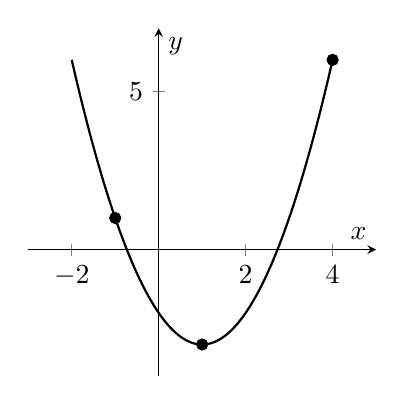
\begin{tikzpicture}
            \begin{axis}[
            xlabel={$x$},
            ylabel={$y$},
            xmin=-3,
            xmax=5,
            ymin=-4,
            ymax=7,
            axis lines=center,
            width=6cm,
            height=6cm]
                \addplot[thick, samples=200, domain=-2:4] {x^2-2*x-2};
                \addplot[
                    color=black,
                    mark=*,
                    only marks
                    ]
                coordinates {
                (-1,1) (1,-3) (4,6)
                };
            \end{axis}
        \end{tikzpicture}
        %\captionof{figure}{Gráfica de la parábola $y=-2-2x+x^2$}
    \end{center}
\end{example}

\newpage

\section{Ejercicios}

\noindent
En los problemas 1 al 16 calcule el determinante.
\begin{tasks}[
    style=enumerate,
    label-offset = 3mm,
    ](2)
    \task $\begin{vmatrix*}[r]7 & 9 & -5 \\ 9 & 3 & 1 \\ -8 & -8 & 10\end{vmatrix*}$
    \task $\begin{vmatrix*}1 & 0 & 3 \\ 0 & 1 & 4 \\ 2 & 1 & 0\end{vmatrix*}$
    \task $\begin{vmatrix*}[r]-1 & 1 & 0 \\ 2 & 1 & 4 \\ 1 & 5 & 6\end{vmatrix*}$
    \task $\begin{vmatrix*}[r]10 & 10 & -8 \\ -7 & 0 & -2 \\ 10 & 6 & 9\end{vmatrix*}$
    \task $\begin{vmatrix*}[r]3 & -1 & 4 \\ 6 & 3 & 5 \\ 2 & -1 & 6\end{vmatrix*}$
    \task $\begin{vmatrix*}[r]-1 & 0 & 6 \\ 0 & 2 & 4 \\ 1 & 2 & -3\end{vmatrix*}$
    \task $\begin{vmatrix*}[r]6 & -10 & 4 \\ 10 & 7 & 5 \\ 3 & 9 & 5\end{vmatrix*}$
    \task $\begin{vmatrix*}[r]-2 & 3 & 1 \\ 4 & 6 & 5 \\ 0 & 2 & 1\end{vmatrix*}$
    \task $\begin{vmatrix*}[r]5 & -2 & 1 \\ 6 & 0 & 3 \\ -2 & 1 & 4\end{vmatrix*}$
    \task $\begin{vmatrix*}[r]-2 & -10 & 7 & 0 \\ 0 & -5 & 4 & -1 \\ 0 & -10 & 0 & 0 \\ 0 & 0 & 0 & 6\end{vmatrix*}$
    \task $\begin{vmatrix*}2 & 0 & 3 & 1 \\ 0 & 1 & 4 & 2 \\ 0 & 0 & 1 & 5 \\ 1 & 2 & 3 & 0\end{vmatrix*}$
    \task $\begin{vmatrix*}[r]-3 & 0 & 0 & 0 \\ -4 & 7 & 0 & 0 \\ 5 & 8 & -1 & 0 \\ 2 & 3 & 0 & 6\end{vmatrix*}$
    \task $\begin{vmatrix*}[r]-6 & 8 & -5 & 0 & 0 \\ 0 & 0 & 0 & 0 & -3 \\ -5 & 0 & -5 & -6 & 0 \\ 0 & -8 & 0 & 0 & 2 \\ 0 & -7 & 0 & 2 & 1\end{vmatrix*}$
    \task $\begin{vmatrix*}[r]2 & 3 & -1 & 4 & 5 \\ 0 & 1 & 7 & 8 & 2 \\ 0 & 0 & 4 & -1 & 5 \\ 0 & 0 & 0 & -2 & 8 \\ 0 & 0 & 0 & 0 & 6\end{vmatrix*}$
    \task $\begin{vmatrix*}[r]0 & 0 & 0 & 0 & 0 \\ 0 & 7 & 0 & 0 & 0 \\ -9 & 1 & 0 & 0 & 0 \\ -6 & 0 & 0 & -2 & -7 \\ 9 & -9 & 0 & -5 & 0\end{vmatrix*}$
    \task $\begin{vmatrix*}[r]-8 & 0 & 0 & -10 & 0 \\ 0 & -8 & 0 & -7 & 1 \\ 0 & 9 & -3 & 0 & -4 \\ -5 & 0 & 7 & 5 & 5 \\ -2 & 0 & -10 & 3 & -7\end{vmatrix*}$
\end{tasks}
\begin{enumerate}[start=17]
    \item Si existe, calcule la matriz inversa de las anteriores matrices mediante la expresión \ref{ADJUNTODEMATRIZ}.
    \item Demuestre que si $A$ y $B$ son matrices diagonales de $n \times n$, entonces $\Det A B=\Det A \Det B$.
    \item Demuestre que si $A$ y $B$ son matrices triangulares inferiores, entonces $A B=\Det A \Det B$.
    \item Demuestre que, en general, no se cumple que $\Det(A+B)=\Det A+\Det B$.
    \item Muestre que si $A$ es triangular, entonces $\Det A \neq 0$ si y sólo si todos los elementos en la diagonal de $A$ son diferentes de cero.
\end{enumerate}
De los problemas 22 al 30 calcule el determinante suponiendo que
$$
\begin{vmatrix*}
a_{11} & a_{12} & a_{13} \\
a_{21} & a_{22} & a_{23} \\
a_{31} & a_{32} & a_{33}
\end{vmatrix*}=8
$$\newpage
\begin{tasks}[
    start=22,
    style=enumerate,
    label-offset = 3mm,
    ](2)
    \task $\begin{vmatrix*}a_{31} & a_{32} & a_{33} \\ a_{21} & a_{22} & a_{23} \\ a_{11} & a_{12} & a_{13}\end{vmatrix*}$
    \task $\begin{vmatrix*}a_{31} & a_{32} & a_{33} \\ a_{11} & a_{12} & a_{13} \\ a_{21} & a_{22} & a_{23}\end{vmatrix*}$
    \task $\begin{vmatrix*}a_{11} & a_{13} & a_{12} \\ a_{21} & a_{23} & a_{22} \\ a_{31} & a_{33} & a_{32}\end{vmatrix*}$
    \task $\begin{vmatrix*}a_{11} & a_{12} & a_{13} \\ 2 a_{21} & 2 a_{22} & 2 a_{23} \\ a_{31} & a_{32} & a_{33}\end{vmatrix*}$
    \task $\begin{vmatrix*}[r]-3 a_{11} & -3 a_{12} & -3 a_{13} \\ 2 a_{21} & 2 a_{22} & 2 a_{23} \\ 5 a_{31} & 5 a_{32} & 5 a_{33}\end{vmatrix*}$
    \task $\begin{vmatrix*}4 a_{11} & -2 a & 3 a_{12} \\ 4 a_{21} & -2 a_{23} & 3 a_{22} \\ 4 a_{31} & -2 a_{33} & 3 a_{32}\end{vmatrix*}$
    \task $\begin{vmatrix*}a_{11} & 2 a_{13} & a_{12} \\ a_{21} & 2 a_{23} & a_{22} \\ a_{31} & 2 a_{33} & a_{32}\end{vmatrix*}$
    \task $\begin{vmatrix*}a_{11} & -a_{12} & a_{12} & a_{13} \\ a_{21} & -a_{22} & a_{22} & a_{23} \\ a_{31} & -a_{32} & a_{32} & a_{33}\end{vmatrix*}$
    \task $\begin{vmatrix*}2 a_{11}-3 a_{21} & 2 a_{12}-3 a_{22} & 2 a_{13}-3 a_{23} \\ a_{31} & a_{32} & a_{33} \\ a_{21} & a_{22} & a_{23}\end{vmatrix*}$
\end{tasks}
\begin{enumerate}[start=31]
    \item Demuestre que si $\alpha$ es un escalar y $A$ es una matriz cuadrada de tamaño $n \times n$, entonces $\Det(\alpha A)=\alpha^n \Det(A)$.
    \item Demuestre que
    $$\begin{vmatrix}
        1+x_1 & x_2 & x_3 & \cdots & x_n \\
        x_1 & 1+x_2 & x_3 & \cdots & x_n \\
        x_1 & x_2 & 1+x_3 & \cdots & x_n \\
        \vdots & \vdots & \vdots & & \vdots \\
        x_1 & x_2 & x_3 & \cdots & 1+x_n
    \end{vmatrix} = 1+x_1+x_2+\cdots+x_n$$
    \item Demuestre que
    $$\begin{vmatrix*}
        \lambda & -1 & 0 & \cdots & 0 & 0 & 0 \\
        0 & \lambda & -1 & \cdots & 0 & 0 & 0 \\
        0 & 0 & \lambda & \ddots & 0 & 0 & 0 \\
        \vdots & \vdots & \vdots & \ddots & \vdots & \vdots & \vdots \\
        0 & 0 & 0 & \cdots & \lambda & -1 & 0 \\
        0 & 0 & 0 & \cdots & 0 & \lambda & -1 \\
        a_0 & a_1 & a_2 & \cdots & a_{n-3} & a_{n-2} & \lambda+a_{n-1}
    \end{vmatrix*}=\lambda^n+a_{n-1} \lambda^{n-1}+a_{n-2} \lambda^{n-2}+\cdots+a_1 \lambda^1+a_0$$
    \item Sea $A$ una matriz de $n \times n$. Demuestre que si la suma de todos los elementos de cada columna de $A$ es cero, entonces $|A|=0$.
    \item Una matriz $A$ es antisimétrica si $A^{T}=-A$ (definición \ref{matriz-antisimetrica}). Si $A$ es una matriz antisimétrica de $n \times n$, demuestre que $\Det A^{T}=(-1)^n \Det A$.
    \item Usando el resultado del problema anterior, demuestre que si $A$ es una matriz antisimétrica de $n \times n$ y $n$ es impar, entonces $\Det A=0$.
    \item Una matriz $A$ se llama ortogonal si $A$ es invertible y $A^{-1}=A^{T}$, es decir, $A^{T} A=A A^{T}=I$. Demuestre que si $A$ es ortogonal, entonces $\Det A= \pm 1$.
    \item La matriz $A$ se llama idempotente si $A^2 = A$ (definición \ref{def:matriz-idempotente}). ¿Cuáles son los valores posibles para $\Det A$ si $A$ es idempotente?
    \item Si es posible, resuelva los sistemas de la página \pageref{EJERCICIOSDECRAMER} usando la regla de Cramer.
\end{enumerate}

\chapter[TRANSFORMACIONES LINEALES]{TRANSFORMACIONES \\ LINEALES}
%\startcontents
\printchaptertableofcontents

Las transformaciones lineales son un pilar esencial en el vasto terreno de las matemáticas, particularmente en el ámbito de álgebra lineal. Para comprender la magnitud de su influencia, es imperativo sumergirse en la esencia misma de estas transformaciones y explorar sus aplicaciones en diversos campos.

Una transformación lineal es, en esencia, una función matemática que preserva la estructura algebraica de los vectores. Al aplicar una transformación lineal a la combinación lineal de dos vectores, los resultados son análogos a la combinación lineal de las transformaciones individuales de cada vector. Este comportamiento de preservación de la linealidad es una característica clave que distingue a las transformaciones lineales y las eleva a una posición central en la teoría algebraica.

%En el fondo de estas transformaciones reside la preservación de las operaciones fundamentales: la suma y la multiplicación por escalares. Cuando aplicamos una transformación lineal a la suma de dos vectores, el resultado es la suma de las transformaciones lineales de cada vector individual. Similarmente, la multiplicación de un vector por un escalar antes de la transformación lineal es equivalente a multiplicar la transformación lineal por ese mismo escalar. Estas propiedades fundamentales son cruciales para entender la coherencia y la estructura que las transformaciones lineales aportan al álgebra lineal.

La aplicabilidad de las transformaciones lineales se extiende a diversos campos de estudio. En el ámbito de la resolución de sistemas de ecuaciones lineales, las transformaciones lineales ofrecen herramientas poderosas para entender y abordar problemas complejos. Además, en el análisis de estructuras algebraicas, como espacios vectoriales y grupos, las transformaciones lineales juegan un papel vital al proporcionar una lente única para examinar las propiedades intrínsecas de estos objetos matemáticos.

Al profundizar en las propiedades y aplicaciones de las transformaciones lineales, se revela un panorama rico y complejo. Desde la diagonalización de matrices hasta la representación canónica de formas cuadráticas, las transformaciones lineales ofrecen un marco conceptual robusto para abordar una variedad de problemas matemáticos.

Las transformaciones lineales no solo son conceptos abstractos en el ámbito de álgebra lineal, sino que constituyen la esencia misma de la coherencia algebraica. Su estudio no solo enriquece nuestra comprensión de las estructuras matemáticas, sino que también desbloquea un conjunto diverso de herramientas analíticas con aplicaciones prácticas significativas.

\section{Definición y ejemplos}

\begin{definition}\label{def:operatorlineal}
    Sean $V$ y $W$ dos espacios vectoriales sobre $K = \RR$. Se dice que una función
    \begin{align*}
        T: V & \longrightarrow W \\
        \mathbb{v} & \longmapsto T\mathbb{v} = \mathbb{w}
    \end{align*}
    es una transformación lineal de $V$ en $W$ si cumple que para cada $\mathbb{u}$, $\mathbb{v} \in V$ y $\alpha \in K$\infoBulle{A una transformación lineal también se le puede llamar operador lineal.}
    \begin{enumerate}[label=\roman*)]
        \item $T(\mathbb{u} + \mathbb{v}) = T\mathbb{u} + T\mathbb{v}$.
        \item $T(\alpha \mathbb{u}) = \alpha T\mathbb{u}$.
    \end{enumerate}
\end{definition}

\begin{notation}
    Se escriben indistintamente $T\mathbb{v}$ y $T(\mathbb{v})$. Denotan lo mismo; las dos se leen “$T$ de $\mathbb{v}$”. Esto es análogo a la notación funcional $f(x)$, que se lee “$f$ de $x$”.
\end{notation}

\begin{observation}
    La notación $T: V \longrightarrow W$ indica que $T$ toma el espacio vectorial real $V$ y lo lleva al espacio vectorial real $W$; esto es, $T$ es una función con $V$ como su dominio y un subconjunto de $W$ como su imagen.
\end{observation}

\begin{example}
    Veamos si
    \begin{align*}
        T: \RR[2] & \longrightarrow \RR[2] \\
        \begin{pmatrix}
            x \\
            y
        \end{pmatrix} & \longmapsto T \begin{pmatrix}
            x \\
            y
        \end{pmatrix} = \begin{pmatrix*}[r]
            x \\
            -y
        \end{pmatrix*}
    \end{align*}
    es una transformación lineal. En este caso, $T: V \longrightarrow W$ es $T: \RR[2] \longrightarrow \RR[2]$, además $\RR[2]$ es un espacio vectorial sobre $\RR$. Notemos que $T$ admite una interpretación geométrica sencilla como se muestra en la figura \ref{HDFDDFHUYFGHFUYGFFGUY}, así se comprueba que $T$ es función. Ahora se tiene\sideFigure[\label{HDFDDFHUYFGHFUYGFFGUY}Transformación de reflexión respecto al eje $x$]{
    \begin{tikzpicture}[scale=0.83]
        \draw[thick,-Stealth] (-1,0) -- (5,0);
        \draw[thick,Stealth-Stealth] (0,-5.5) -- (0,5.5);
        \draw[dash pattern=on 3pt off 3pt] (0,4) node[left] {$y$} -- (4,4) -- (4,-4) -- (0,-4) node[left] {$-y$};
        \draw[thick,-latex] (0,0) -- (4,4) node[above] {$\begin{pmatrix}
            x \\
            y
        \end{pmatrix}$};
        \draw[thick,-latex] (0,0) -- (4,-4) node[below] {$\begin{pmatrix*}[r]
            x \\
            -y
        \end{pmatrix*}$};
        \node at (0,0) [below left] {$\mathbb{0}$};
        \node at (4,0) [above right] {$x$};
        \node at (2,2) [above,rotate=45] {$\mathbb{u}$};
        \node at (2,-2) [below,rotate=-45] {$\mathbb{w} = T\mathbb{u}$};
    \end{tikzpicture}
    }
    \begin{enumerate}[label=\roman*)]
        \item Sea $\mathbb{u}$, $\mathbb{v} \in \RR[2]$ con $\mathbb{u} = \begin{pmatrix}
            x_1 \\
            y_1
        \end{pmatrix}$, $\mathbb{v} = \begin{pmatrix}
            x_2 \\
            y_2
        \end{pmatrix}$. Entonces
        \begin{align*}
            T(\mathbb{u} + \mathbb{v}) & = T\left( \begin{pmatrix}
                x_1 \\
                y_1
            \end{pmatrix} + \begin{pmatrix}
                x_2 \\
                y_2
            \end{pmatrix} \right) \\
            & = T \begin{pmatrix}
                x_1 + x_2 \\
                y_1 + y_2
            \end{pmatrix} \\
            & = \begin{pmatrix}
                x_1 + x_2 \\
                -(y_1 + y_2)
            \end{pmatrix} \\
            & = \begin{pmatrix}
                x_1 + x_2 \\
                -y_1 + (-y_2)
            \end{pmatrix} \\
            & = \begin{pmatrix*}[r]
                x_1 \\
                -y_1
            \end{pmatrix*} + \begin{pmatrix*}[r]
                x_2 \\
                -y_2
            \end{pmatrix*} \\
            & = T\mathbb{u} + T\mathbb{v}
        \end{align*}
        Por tanto $T(\mathbb{u} + \mathbb{v}) = T\mathbb{u} + T\mathbb{v}$.\newpage
        \item Sea $\mathbb{u} \in \RR[2]$ con $\mathbb{u} = \begin{pmatrix}
            x_1 \\
            y_1
        \end{pmatrix}$ y $\alpha \in \RR$. Entonces
        \begin{align*}
            T(\alpha \mathbb{u}) & = T \left( \alpha \begin{pmatrix}
                x_1 \\
                y_1
            \end{pmatrix} \right) \\
            & = T \begin{pmatrix}
                \alpha x_1 \\
                \alpha y_1
            \end{pmatrix} \\
            & = \begin{pmatrix*}[r]
                \alpha x_1 \\
                - \alpha y_1
            \end{pmatrix*} \\
            & = \alpha \begin{pmatrix*}[r]
                x_1 \\
                -y_1
            \end{pmatrix*} \\
            & = \alpha T \mathbb{u}
        \end{align*}
        Por tanto, $T(\alpha \mathbb{u}) = \alpha T\mathbb{u}$.
    \end{enumerate}
    Por tanto, $T$ es una transformación lineal de $\RR[2]$ a $\RR[2]$.
\end{example}

\begin{example}
    Supongamos que el vector $\mathbb{v}$ se rota un ángulo $\theta$ (medido en grados o radianes) en sentido contrario al de las manecillas del reloj. Llamemos a este nuevo vector rotado $\mathbb{v}'$. Entonces como se ve en la figura \ref{fig:rotado1}, si $r$ denota la longitud de $\mathbb{v}$, entonces\sideFigure[\label{fig:rotado1}Transformación de rotación]{
    \begin{center}
        \begin{tikzpicture}[scale=0.76]
            \coordinate (A) at (0,0);
            \draw[-Stealth,thick] (-1,0) -- (5.5,0) node[right] {$x$} coordinate (B);
            \draw[-Stealth,thick] (0,-1) -- (0,5.5) node[above] {$y$};
            \draw[dash pattern=on 3pt off 3pt,thin] (3,0) -- (3,4) -- (0,4);
            \draw[dash pattern=on 3pt off 3pt,thin] (4.2,0) -- (4.2,1.6) -- (0,1.6);
            \draw[-latex,thick] (0,0) -- (3,4) coordinate(D);
            \draw[-latex,thick] (0,0) -- (4.2,1.6) coordinate(C);
            \node at (3,4) [right] {$\mathbb{v}' = \begin{pmatrix}
                x' \\
                y'
            \end{pmatrix}$};
            \node at (4.2,1.6) [right] {$\mathbb{v} = \begin{pmatrix}
                x \\
                y
            \end{pmatrix}$};
            \pic[draw, -latex, "$\alpha$", angle eccentricity=1.3,angle radius=1cm] {angle = B--A--C};
            \pic[draw, -latex, "$\theta$", angle eccentricity=1.3,angle radius=0.8cm] {angle = C--A--D};
            \pic[draw, -latex, "$\theta + \alpha$", angle eccentricity=1.3,angle radius=1.55cm] {angle = B--A--D};
            \node at (0,0) [below left] {$\mathbb{0}$};
        \end{tikzpicture}
    \end{center}
    }
    \marginElement{\justify
    \begin{center}
        \colorbox{gray!20}{\parbox[c]{\dimexpr\linewidth-3pt-2\fboxsep-2\fboxrule}{
            La transformación lineal de rotación es un proceso matemático que gira un objeto alrededor de un punto fijo. En un espacio bidimensional, la rotación se puede describir mediante matrices de rotación como
            $$\begin{pmatrix}
                x' \\
                y'
            \end{pmatrix} = \begin{bmatrix*}[r]
                \cos \theta & - \sen \theta \\
                \sen \theta & \cos \theta
            \end{bmatrix*} \begin{bmatrix}
                x \\
                y
            \end{bmatrix}$$
            Estas matrices aplican operaciones lineales para cambiar las coordenadas del objeto y lograr la rotación deseada. La trigonometría es fundamental en la formulación de estas matrices, y la aplicación repetida de rotaciones puede dar lugar a transformaciones más complejas.
        }}
    \end{center}
    }
    \begin{equation}
        x = r \cos(\alpha), \quad y = r \sen(\alpha)
    \end{equation}
    y
    \begin{equation}
        x' = r \cos(\theta + \alpha), \quad y' = r \sen(\theta + \alpha)
    \end{equation}
    Entonces
    \begin{align*}
        x' & = r \big( \cos(\theta) \cos(\alpha) - \sen(\theta) \sen(\alpha) \big) \\
        & = r \cos(\theta) \cos(\alpha) - r \sen(\theta) \sen(\alpha) \\
        & = x \cos(\theta) - y \sen(\theta)
    \end{align*}
    De manera análoga,
    \begin{align*}
        y' & = \big( \cos(\theta) \sen(\alpha) + \cos(\alpha) \sen(\theta) \big) \\
        & = r \cos(\theta) \sen(\alpha) + r \cos(\alpha) \sen(\theta) \\
        & = y \cos(\theta) + x \sen(\theta)
    \end{align*}
    Así pues, sea
    \begin{align*}
        T: \RR[2] & \longrightarrow \RR[2] \\
        \begin{pmatrix}
            x \\
            y
        \end{pmatrix} & \longmapsto T \begin{pmatrix}
            x \\
            y
        \end{pmatrix} = \begin{pmatrix}
            x \cos \theta - y \sen \theta \\
            x \sen \theta + y \cos \theta
        \end{pmatrix}
    \end{align*}
    con $0 \leq \theta < 2 \pi$ y $r > 0$ donde $r = \sqrt{x^2+y^2}$. Probemos que $T$ es transformación lineal:
    \begin{enumerate}[label=\roman*)]
        \item Sea $\mathbb{u}$, $\mathbb{v} \in \RR[2]$ con $\mathbb{u} = \begin{pmatrix}
            x \\
            y
        \end{pmatrix}$, $\mathbb{v} = \begin{pmatrix}
            x' \\
            y'
        \end{pmatrix}$. Entonces
        \begin{align*}
            T(\mathbb{u} + \mathbb{v}) & = T \begin{pmatrix}
                x + x' \\
                y + y'
            \end{pmatrix} \\
            & = \begin{pmatrix}
                (x + x') \cos \theta - (y + y') \sen \theta \\
                (x + x') \sen \theta + (y + y') \cos \theta
            \end{pmatrix} \\
            & = \begin{pmatrix}
                x \cos \theta + x' \cos \theta - y \sen \theta - y' \sen \theta \\
                x \sen \theta + x' \sen \theta + y \cos \theta + y' \cos \theta
            \end{pmatrix} \\
            & = \begin{pmatrix}
                x \cos \theta - y \sen \theta \\
                x \sen \theta + y \cos \theta
            \end{pmatrix} + \begin{pmatrix}
                x' \cos \theta - y' \sen \theta \\
                x' \sen \theta - y' \cos \theta
            \end{pmatrix} \\
            & = T\mathbb{u} + T\mathbb{v}
        \end{align*}
        Por tanto $T(\mathbb{u} + \mathbb{v}) = T\mathbb{u} + T\mathbb{v}$.
        \item Se deja como ejercicio al lector.
    \end{enumerate}
    Por tanto, $T$ es una transformación lineal de $\RR[2]$ a $\RR[2]$.
\end{example}

\begin{example}
    Veamos si
    \begin{align*}
        T: \RR[2] & \longrightarrow \RR[3] \\
        \begin{pmatrix}
            x \\
            y
        \end{pmatrix} & \longmapsto T \begin{pmatrix}
            x \\
            y
        \end{pmatrix} = \begin{pmatrix}
            x + y \\
            x - y \\
            2y
        \end{pmatrix}
    \end{align*}
    es una transformación lineal.
    \begin{enumerate}[label=\roman*)]
        \item Sea $\mathbb{u}$, $\mathbb{v} \in \RR[2]$ con $\mathbb{u} = \begin{pmatrix}
            x_1 \\
            y_1
        \end{pmatrix}$, $\mathbb{v} =  \begin{pmatrix}
            x_2 \\
            y_2
        \end{pmatrix}$. Entonces
        \begin{align*}
            T(\mathbb{u} + \mathbb{v}) & = T \left( \begin{pmatrix}
                x_1 \\
                y_1
            \end{pmatrix} + \begin{pmatrix}
                x_2 \\
                y_2
            \end{pmatrix} \right) \\
            & = T \begin{pmatrix}
                x_1 + x_2 \\
                y_1 + y_2
            \end{pmatrix} \\
            & = \begin{pmatrix}
                x_1 + x_2 + y_1 + y_2 \\
                x_1 + x_2 - (y_1 + y_2) \\
                2(y_1 + y_2)
            \end{pmatrix} \\
            & = \begin{pmatrix}
                x_1 + y_1 + x_2 + y_2 \\
                x_1 - y_1 + x_2 - y_2 \\
                2y_1 + 2y_2
            \end{pmatrix} \\
            & = \begin{pmatrix}
                x_1 + y_1 \\
                x_1 - y_1 \\
                2y_1
            \end{pmatrix} + \begin{pmatrix}
                x_2 + y_2 \\
                x_2 - y_2 \\
                2y_2
            \end{pmatrix} \\
            & = T\mathbb{u} + T\mathbb{v}
        \end{align*}
        Por tanto $T(\mathbb{u} + \mathbb{v}) = T\mathbb{u} + T\mathbb{v}$.
        \item Sea $\mathbb{u} \in \RR[2]$ con $\mathbb{u} = \begin{pmatrix}
            x_1 \\
            y_1
        \end{pmatrix}$ y $\alpha \in \RR$. Entonces
        \begin{align*}
            T(\alpha \mathbb{u}) & = T \left( \alpha \begin{pmatrix}
                x_1 \\
                y_1
            \end{pmatrix} \right) \\
            & = T \begin{pmatrix}
                \alpha x_1 \\
                \alpha y_1
            \end{pmatrix} \\
            & = \begin{pmatrix}
                \alpha x_1 + \alpha y_1 \\
                \alpha x_1 - \alpha y_1 \\
                2 \alpha y_1
            \end{pmatrix} \\
            & = \alpha \begin{pmatrix}
                x_1 + y_1 \\
                x_1 - y_1 \\
                2 y_1
            \end{pmatrix} \\
            & = \alpha T \mathbb{u}
        \end{align*}
        Por tanto, $T(\alpha \mathbb{u}) = \alpha T\mathbb{u}$.
    \end{enumerate}
    Por tanto, $T$ es una transformación lineal de $\RR[2]$ a $\RR[3]$.
\end{example}

\begin{definition}
    A la transformación lineal dada por $\mathcal{O} \mathbb{u} = \mathbb{0}_{W}$, $\forall \mathbb{u} \in V$ siendo $\mathcal{O}:V \longrightarrow W$, se le llama transformación cero.
\end{definition}

\begin{definition}
    A la transformación lineal dada por $I \mathbb{u} = \mathbb{u}$, $\forall \mathbb{u} \in V$ siendo $I:V \longrightarrow V$, se le llama transformación identidad.
\end{definition}

\begin{example}
    Sea $T: \RR[n] \longrightarrow \RR[m]$ definida como
    $$T\mathbb{x} = A\mathbb{x}$$
    siendo $A \in \matrizmn$. Verifique que $T$ es una transformación lineal. \\
    \solucion Sea
    \begin{align*}
        T: \RR[n] & \longrightarrow \RR[m] \\
        \mathbb{x} & \longmapsto T\mathbb{x} = A\mathbb{x}
    \end{align*}
    Probemos que $T$ es una transformación lineal:
    \begin{enumerate}[label=\roman*)]
        \item Sea $\mathbb{x}$, $\mathbb{y} \in \RR[n]$. Entonces
        \begin{align*}
            T(\mathbb{x} + \mathbb{y}) & = A(\mathbb{x} + \mathbb{y}) \\
            & = A\mathbb{x} + \mathbb{y} \\
            & = T\mathbb{x} + T\mathbb{y}
        \end{align*}
        Por tanto $T(\mathbb{x} + \mathbb{y}) = T\mathbb{x} + T\mathbb{y}$.
        \item Sea $\mathbb{x} \in \RR[n]$ y $\alpha \in \RR$. Entonces
        \begin{align*}
            T(\alpha \mathbb{x}) & = A(\alpha \mathbb{x}) \\
            & = \alpha A \mathbb{x} \\
            & = \alpha T \mathbb{x}
        \end{align*}
        Por tanto, $T(\alpha \mathbb{x}) = \alpha T\mathbb{x}$.
    \end{enumerate}
    Por tanto, $T$ es una transformación lineal de $\RR[n]$ a $\RR[m]$.
\end{example}

\begin{example}
    Sea
    \begin{align*}
        T:C[0,  1] & \longrightarrow \RR \\
        f & \longmapsto T_{f} = \int_0^1 f(x) dx
    \end{align*}
    donde $C[0,  1]$ es el conjunto de funciones $f:[0,  1] \longrightarrow \RR$ continuas. Notemos que $T$ admite una interpretación geométrica sencilla, tomando una función arbitraria en $C[0,  1]$ como se muestra en la figura \ref{IDIDIIDKDKDKKK}. Así pues, comprobemos que $T$ es una transformación lineal:\sideFigure[\label{IDIDIIDKDKDKKK}Operador integral]{
    \begin{center}
        \begin{tikzpicture}[declare function={
        a=0;
        b=3;
        f(\x)=exp(\x) - \x + 1;
        }]
            \begin{axis}[
            axis lines=middle,
            xlabel=$x$,
            ylabel=$y$,
            xmin=-0.5,
            xmax=3,
            ymin=-0.75,
            ymax=8,
            ytick=\empty,
            xtick={2},
            xticklabels={$1$},
            width=6.3cm,
            height=10cm,
            xlabel style={
                anchor=west,
            },
            ylabel style={
                anchor=south,
            },
            axis line style={thick,-Stealth},
            ]
                \addplot[name path=A, gray, thick, domain=0.01:2, smooth] {f(x)};
                \path[name path=B] (\pgfkeysvalueof{/pgfplots/xmin},0) -- (\pgfkeysvalueof{/pgfplots/xmax},0);
                \addplot[gray!20] fill between [of=A and B, soft clip={domain=a:2},];
                \addplot[dashed, thick,->,>={}] coordinates {(2,0)(2,8)};
                \path ({(2+a)/2},{f((2+a)/2)/2}) node{$\displaystyle \int_0^1 f(x)$};
                \path (0,0) node[below left] {$0$};
                \addplot[thick,->,>={}] coordinates {(0,6)(0,0)(2.5,0)};
            \end{axis}
        \end{tikzpicture}
    \end{center}
    }
    \begin{enumerate}[label=\roman*)]
        \item Sea $f$, $g \in C[0,  1]$. Entonces
        \begin{align*}
            T(f + g) & = \int_0^1 (f + g)(x) dx \\
            & = \int_0^1 f(x) + g(x) dx \\
            & = \int_0^1 f(x) dx + \int_0^1 g(x) dx \\
            & = T_{f} + T_{g}
        \end{align*}
        Por tanto, $T(f + g) = T_{f} + T_{g}$.
        \item[ii)] Sea $f \in C[0,  1]$ y $\alpha \in \RR$. Entonces
        \begin{align*}
            T(\alpha f) & = \int_0^1 (\alpha f)(x) dx \\
            & = \int_0^1 \alpha f(x) dx \\
            & = \alpha \int_0^1 f(x) dx \\
            & = \alpha T_{f}
        \end{align*}
        Por tanto, $T(\alpha f) = \alpha T_{f}$.
    \end{enumerate}
    Por tanto, $T$ es una transformación lineal.
\end{example}

\begin{example}
    Sea
    \begin{align*}
        T:C[0,  1] & \longrightarrow \RR \\
        f & \longmapsto T_{f} = f(0) + 1
    \end{align*}
    donde $C[0,  1]$ es el conjunto de funciones $f:[0,  1] \longrightarrow \RR$ continuas. Notemos que $T$ es no lineal, pues tenemos que
    $$T(f + g) = (f + g) + 1 = f(0) + g(0) + 1$$
    y
    $$T_{f} + T_{g} = [f(0) + 1] + [g(0) + 1] = f(0) + g(0) + 2$$
\end{example}

\begin{theorem}
    Sean $V$ y $W$ espacios vectoriales sobre $K$. Si $T: V \longrightarrow W$ es una transformación lineal, entonces
    \begin{enumerate}[label=\roman*)]
        \item $T\mathbb{0}_V = \mathbb{0}_W$.
        \item $T(-\mathbb{u}) = -T\mathbb{u}$.
        \item $T(\mathbb{u} - \mathbb{v}) = T\mathbb{u} - T\mathbb{v}$.
        \item $T(\alpha_1 \mathbb{u}_1 + \alpha_2 \mathbb{u}_2 + \cdots + \alpha_n \mathbb{u}_n) = \alpha_1 T\mathbb{u}_1 + \alpha_2 T\mathbb{u}_2 + \cdots + \alpha_n T\mathbb{u}_n$ con $\alpha_1$, $\alpha_2$, $\dots$, $\alpha_n \in K$ y $\mathbb{u}_1$, $\mathbb{u}_2$, $\dots$, $\mathbb{u}_n \in V$.
    \end{enumerate}
    \demostracion
    \begin{enumerate}[label=\roman*)]
        \item Tenemos que
        $$\mathbb{0}_V = \mathbb{0}_V + \mathbb{0}_V$$
        así que
        \begin{align*}
            T\mathbb{0}_V & = T(\mathbb{0}_V + \mathbb{0}_V) \\
            & = T\mathbb{0}_V + T\mathbb{0}_V
        \end{align*}
        Ahora
        \begin{align*}
            \mathbb{0}_W & = T\mathbb{0}_V + (-T\mathbb{0}_V) \\
            & = T\mathbb{0}_V + T\mathbb{0}_V + (-T\mathbb{0}_V) \\
            & = T\mathbb{0}_V + \big( T\mathbb{0}_V + (-T\mathbb{0}_V) \big) \\
            & = T\mathbb{0}_V + \mathbb{0}_W \\
            & = T\mathbb{0}_V
        \end{align*}
        Por tanto, $T\mathbb{0}_V = \mathbb{0}_W$.
        \item Sea $\mathbb{u} \in V$, entonces
        \begin{align*}
            T\mathbb{u} + T(-\mathbb{u}) & = T\big( \mathbb{u} + (-\mathbb{u}) \big) \\
            & = T(\mathbb{0}_V) \\
            & = \mathbb{0}_W
        \end{align*}
        Por tanto, $T(-\mathbb{u}) = -T\mathbb{u}$.
        \item Sean $\mathbb{u}$, $\mathbb{v} \in V$, entonces
        \begin{align*}
            T(\mathbb{u} - \mathbb{v}) & = T\mathbb{u} + T(-\mathbb{v}) \\
            & = T\mathbb{u} - T\mathbb{v}
        \end{align*}
        Por tanto, $T(\mathbb{u} - \mathbb{v}) = T\mathbb{u} - T\mathbb{v}$.
        \item Sean $\alpha_1$, $\alpha_2$, $\dots$, $\alpha_n \in K$ y sean $\mathbb{u}_1$, $\mathbb{u}_2$, $\dots$, $\mathbb{u}_n \in V$. Procedamos por inducción sobre $n$. Si $n = 2$, entonces
        \begin{align*}
            T(\alpha_1 \mathbb{u}_1 + \alpha_2 \mathbb{u}_2) & = T(\alpha_1 \mathbb{u}_1) + T(\alpha_2 \mathbb{u}_2) \\
            & = \alpha_1 T\mathbb{u}_1 + \alpha_2 T\mathbb{u}_2
        \end{align*}
        Supongamos que se cumple para $k$, es decir,
        $$T(\alpha_1 \mathbb{u}_1 + \alpha_2 \mathbb{u}_2 + \cdots + \alpha_k \mathbb{u}_k) = \alpha_1 T\mathbb{u}_1 + \alpha_2 T\mathbb{u}_2 + \cdots + \alpha_k T\mathbb{u}_k$$
        Probemos ahora para $k+1$,
        \begin{align*}
            T(\alpha_1 \mathbb{u}_1 + \alpha_2 \mathbb{u}_2 + \cdots + \alpha_k \mathbb{u}_k + \alpha_{k+1} \mathbb{u}_{k+1}) & = T(\alpha_1 \mathbb{u}_1 + \alpha_2 \mathbb{u}_2 + \cdots + \alpha_k \mathbb{u}_k) + T(\alpha_{k+1} \mathbb{u}_{k+1}) \\
            & = \alpha_1 T\mathbb{u}_1 + \alpha_2 T\mathbb{u}_2 + \cdots + \alpha_k T\mathbb{u}_k + \alpha_{k+1} T\mathbb{u}_{k+1}
        \end{align*}
        Por tanto,
        $$T(\alpha_1 \mathbb{u}_1 + \alpha_2 \mathbb{u}_2 + \cdots + \alpha_n \mathbb{u}_n) = \alpha_1 T\mathbb{u}_1 + \alpha_2 T\mathbb{u}_2 + \cdots + \alpha_n T\mathbb{u}_n$$
    \end{enumerate}
\end{theorem}

\begin{theorem}\label{theorem:LAKAAKLKSKSKSSIIS}
    Sean $V$ y $W$ dos espacios vectoriales sobre $K$ y sean $T_1$, $T_2:V \longrightarrow W$ dos transformaciones lineales tales que
    $$T_1(\mathbb{v}_i) = T_2(\mathbb{v}_i), \text{ para } i = 1,  2,  \dots,  n$$
    siendo $\{ \mathbb{v}_1,  \mathbb{v}_2,  \dots,  \mathbb{v}_n \}$ una base de $V$, entonces $T_1 = T_2$. \\
    \demostracion
    Sea $\{ \mathbb{v}_1,  \mathbb{v}_2,  \dots,  \mathbb{v}_n \}$ una base de $V$. Basta probar que
    $$T_1\mathbb{v} = T_2 \mathbb{v}, \forall \mathbb{v} \in V$$
    Así pues, sea $\mathbb{v} \in V$ un elemento arbitrario, entonces
    \begin{equation}
        \mathbb{v} = \alpha_1 \mathbb{v}_1 + \alpha_2 \mathbb{v}_2 + \cdots + \alpha_n \mathbb{v}_n \label{JAJJSJSKSKDKKSKDSKDKIDD}
    \end{equation}
    con $\alpha_i \in K$ para $i = 1$, $2$, $\dots$, $n$, ya que $\{ \mathbb{v}_1,  \mathbb{v}_2,  \dots,  \mathbb{v}_n \}$ es una base de $V$. De \eqref{JAJJSJSKSKDKKSKDSKDKIDD},
    \begin{align*}
        T_1 \mathbb{v} & = T_1(\alpha_1 \mathbb{v}_1 + \alpha_2 \mathbb{v}_2 + \cdots + \alpha_n \mathbb{v}_n) \\
        & = T_1(\alpha_1 \mathbb{v}_1) + T_1(\alpha_2 \mathbb{v}_2) + \cdots + T_1(\alpha_n \mathbb{v}_n) \\
        & = \alpha_1 T_1 \mathbb{v}_1 + \alpha_2 T_1 \mathbb{v}_2 + \cdots + \alpha_n T_1 \mathbb{v}_n \\
        & = \alpha_1 T_2 \mathbb{v}_1 + \alpha_2 T_2 \mathbb{v}_2 + \cdots + \alpha_n T_2 \mathbb{v}_n \\
        & = T_2(\alpha_1 \mathbb{v}_1) + T_2(\alpha_2 \mathbb{v}_2) + \cdots + T_2(\alpha_n \mathbb{v}_n) \\
        & = T_2(\alpha_1 \mathbb{v}_1 + \alpha_2 \mathbb{v}_2 + \cdots + \alpha_n \mathbb{v}_n) \\
        & = T_2 \mathbb{v}
    \end{align*}
    Por tanto, $T_1 \mathbb{v} = T_2 \mathbb{v}$, $\forall \mathbb{v} \in V$. Así, $T_1 = T_2$.
\end{theorem}

\section{Núcleo e imagen de una transformación lineal}

\begin{definition}
    Sean $V$ y $W$ espacios vectoriales sobre $K$ y $T:V \longrightarrow W$ una transformación lineal. Se define:
    \begin{enumerate}[label=\roman*)]
        \item El núcleo de la transformación lineal $T$, como
        $$\Nuc(T) = \left\{ \mathbb{v} \in V \mid T\mathbb{v} = \mathbb{0}_W \right\}$$
        \item La imagen de la transformación lineal $T$, como
        $$\Ima(T) = \left\{ \mathbb{w} \in W \mid T\mathbb{v} = \mathbb{w}, \text{ para algún } \mathbb{v} \in V \right\}$$
        \item La nulidad de la transformación lineal $T$, como
        $$\nu(T) = \Dim \big( \Nuc(T) \big)$$
        \item El rango de la transformación lineal $T$, como
        $$\rho(T) = \Dim \big( \Ima(T) \big)$$
    \end{enumerate}
\end{definition}

\newpage

\begin{theorem}
    Sean $V$ y $W$ espacios vectoriales sobre $K$ y $T:V \longrightarrow W$ una transformación lineal, entonces $\Nuc(T)$ es subespacio de $V$ e $\Ima(T)$ es subespacio de $W$. \\
    \demostracion
    Primero, probemos que $\Nuc(T)$ es subespacio de $V$. Sean $\mathbb{v}_1$, $\mathbb{v}_2 \in \Nuc(T)$ y $\alpha \in K$, entonces
    \begin{equation}
        T\mathbb{v}_1 = \mathbb{0}_W \quad \text{ y } \quad T\mathbb{v}_2 = \mathbb{0}_W
    \end{equation}
    Así,
    \begin{align*}
        T(\mathbb{v}_1 + \mathbb{v}_2) & = T\mathbb{v}_1 + T\mathbb{v}_2 \\
        & = \mathbb{0}_W + \mathbb{0}_W \\
        & = \mathbb{0}_W
    \end{align*}
    Entonces
    \begin{equation}
        \mathbb{v}_1 + \mathbb{v}_2 \in \Nuc(T) \label{JAUDJKDKDKDKD}
    \end{equation}
    Además
    \begin{align*}
        T(\alpha \mathbb{v}_1) & = \alpha T\mathbb{v}_1 \\
        & = \alpha \mathbb{0}_W \\
        & = \mathbb{0}_W
    \end{align*}
    Entonces
    \begin{equation}
        \alpha \mathbb{v}_1 \in \Nuc(T) \label{OSPWPEOSLDDPDPD}
    \end{equation}
    Por tanto, de \eqref{JAUDJKDKDKDKD} y \eqref{OSPWPEOSLDDPDPD}, $\Nuc(T)$ es subespacio de $V$.

    Ahora veamos que $\Ima(T)$ es subespacio de $W$. Sean $\mathbb{w}_1$, $\mathbb{w}_2 \in \Ima(T)$ y $\alpha \in K$, entonces
    \begin{equation}
        \mathbb{w}_1 = T\mathbb{v}_1, \text{ para algún } \mathbb{v}_1 \in V \quad \text{ y } \quad \mathbb{w}_2 = T\mathbb{v}_2, \text{ para algún } \mathbb{v}_2 \in V
    \end{equation}
    Así,
    \begin{align*}
        \mathbb{w}_1 + \mathbb{w}_2 & = T\mathbb{v}_1 + T\mathbb{v}_2 \\
        & = T(\mathbb{v}_1 + \mathbb{v}_2) \\
        & = T\mathbb{\mu}
    \end{align*}
    siendo $\mathbb{\mu} = \mathbb{v}_1 + \mathbb{v}_2$. Entonces
    \begin{equation}
        \mathbb{w}_1 + \mathbb{w}_2 \in \Ima(T) \label{IAISISKSKSKLS}
    \end{equation}
    Además
    \begin{align*}
        \alpha \mathbb{w}_1 & = \alpha T\mathbb{v}_1 \\
        & = T(\alpha \mathbb{v}_1) \\
        & = T(\mathbb{\upsilon})
    \end{align*}
    siendo $\mathbb{\upsilon} = \alpha \mathbb{v}_1$. Entonces
    \begin{equation}
        \alpha \mathbb{w}_1 \in \Ima(T) \label{ISOSPPSOSPASHSHSJ}
    \end{equation}
    Por tanto, de \eqref{IAISISKSKSKLS} y \eqref{ISOSPPSOSPASHSHSJ} $\Ima(T)$ es subespacio de $W$.
\end{theorem}

\begin{example}
    Dada la transformación lineal $T:\RR[4] \longrightarrow \RR[2]$ definida por
    $$T\begin{pmatrix}
        x \\
        y \\
        z \\
        w
    \end{pmatrix} = \begin{pmatrix}
        x + z \\
        y + w
    \end{pmatrix}$$
    Determine $\Nuc(T)$, $\Ima(T)$, $\nu(T)$ y $\rho(T)$. \newpage
    \solucion Por definición,
    \begin{align*}
        \Nuc(T) & = \left\{ \begin{pmatrix}
            x \\
            y \\
            z \\
            w
        \end{pmatrix} \in \RR[4] \mid T \begin{pmatrix}
            x \\
            y \\
            z \\
            w
        \end{pmatrix} = \begin{pmatrix}
            0 \\
            0
        \end{pmatrix} \right\} \\
        & = \left\{ \begin{pmatrix}
            x \\
            y \\
            z \\
            w
        \end{pmatrix} \in \RR[4] \mid \begin{pmatrix}
            x + z \\
            y + w
        \end{pmatrix} = \begin{pmatrix}
            0 \\
            0
        \end{pmatrix} \right\} \\
        & = \left\{ \begin{pmatrix}
            x \\
            y \\
            z \\
            w
        \end{pmatrix} \in \RR[4] \mid x + z = 0, \; y + w = 0 \right\} \\
        & = \left\{ \begin{pmatrix*}[r]
            x \\
            y \\
            -x \\
            -y
        \end{pmatrix*} \in \RR[4] \mid x,  y \in \RR \right\} \\
        & = \left\{ x \begin{pmatrix*}[r]
            1 \\
            0 \\
            -1 \\
            0
        \end{pmatrix*} + y \begin{pmatrix*}[r]
            0 \\
            1 \\
            0 \\
            -1
        \end{pmatrix*} \mid x,  y \in \RR \right\}
    \end{align*}
    Por tanto,
    $$\Nuc(T) = \Gen \left( \left\{ \begin{pmatrix*}[r]
        1 \\
        0 \\
        -1 \\
        0
    \end{pmatrix*},  \begin{pmatrix*}[r]
        0 \\
        1 \\
        0 \\
        -1
    \end{pmatrix*} \right\} \right)$$
    y como los vectores son l.i, entonces $\nu(T) = 2$. Ahora, por definición,
    \begin{align*}
        \Ima(T) & = \left\{ \begin{pmatrix}
            \gamma_1 \\
            \gamma_2
        \end{pmatrix} \in \RR[2] \mid T\begin{pmatrix}
            x \\
            y \\
            z \\
            w
        \end{pmatrix} = \begin{pmatrix}
            \gamma_1 \\
            \gamma_2
        \end{pmatrix}, \text{ para algún } \begin{pmatrix}
            x \\
            y \\
            z \\
            w
        \end{pmatrix} \in \RR[4] \right\} \\
        & = \left\{ \begin{pmatrix}
            \gamma_1 \\
            \gamma_2
        \end{pmatrix} \in \RR[2] \mid \begin{pmatrix}
            x + z \\
            y + w
        \end{pmatrix} = \begin{pmatrix}
            \gamma_1 \\
            \gamma_2
        \end{pmatrix}, \text{ para algún } \begin{pmatrix}
            x \\
            y \\
            z \\
            w
        \end{pmatrix} \in \RR[4] \right\} \\
        & = \left\{ \begin{pmatrix}
            \gamma_1 \\
            \gamma_2
        \end{pmatrix} = \begin{pmatrix}
            x + z \\
            y + w
        \end{pmatrix}, \text{ para algún } \begin{pmatrix}
            x \\
            y \\
            z \\
            w
        \end{pmatrix} \in \RR[4] \right\} \\
        & = \left\{ \begin{pmatrix}
            \gamma_1 \\
            \gamma_2
        \end{pmatrix} = x \begin{pmatrix}
            1 \\
            0
        \end{pmatrix} + y \begin{pmatrix}
            0 \\
            1
        \end{pmatrix} + z \begin{pmatrix}
            1 \\
            0
        \end{pmatrix} + w \begin{pmatrix}
            0 \\
            1
        \end{pmatrix}, \text{ para algún } x,  y,  z,  w \in \RR \right\} \\
        & = \left\{ \begin{pmatrix}
            \gamma_1 \\
            \gamma_2
        \end{pmatrix} = x \begin{pmatrix}
            1 \\
            0
        \end{pmatrix} + y \begin{pmatrix}
            0 \\
            1
        \end{pmatrix} + z \begin{pmatrix}
            1 \\
            0
        \end{pmatrix} + w \begin{pmatrix}
            0 \\
            1
        \end{pmatrix}, \text{ para algún } x,  y,  z,  w \in \RR \right\}
    \end{align*}
    Por tanto,
    $$\Ima(T) = \Gen \left( \left\{  \begin{pmatrix}
        1 \\
        0
    \end{pmatrix},  \begin{pmatrix}
        0 \\
        1
    \end{pmatrix},  \begin{pmatrix}
        1 \\
        0
    \end{pmatrix},  \begin{pmatrix}
        0 \\
        1
    \end{pmatrix} \right\} \right)$$
    y en este caso, vemos que solo dos vectores son l.i, así que $\rho(T) = 2$.
\end{example}

\begin{example}
    Sea $T: P_3(x) \longrightarrow P_2(x)$ una transformación lineal definida por
    $$Tp(x) = T \left( a_3x^3 + a_2x^2 + a_1x + a_0 \right) = a_2x^2 + a_1x + a_0$$
    Determine $\Nuc(T)$, $\Ima(T)$, $\nu(T)$ y $\rho(T)$. \newpage
    \solucion Por definición,
    \begin{align*}
        \Nuc(T) & = \left\{ p(x) \in P_3(x) \mid Tp(x) = 0 \right\} \\
        & = \left\{ p(x) \in P_3(x) \mid T \left( a_3x^3 + a_2x^2 + a_1x + a_0 \right) = 0 \right\} \\
        & = \left\{ p(x) \in P_3(x) \mid a_2x^2 + a_1x + a_0 = 0 \right\} \\
        & = \left\{ p(x) \in P_3(x) \mid a_0 = 0,  a_1 = 0,  a_2 = 0 \right\} \\
        & = \left\{ a_3x^3 + 0 \cdot x^2 + 0 \cdot x + 0 \cdot 0 \mid a_3 \in \RR \right\} \\
        & = \left\{ a_3x^3 \mid a_3 \in \RR \right\} \\
        & = \Gen \left( \left\{ x^3 \right\} \right)
    \end{align*}
    Por tanto,
    $$\Nuc(T) = \Gen \left( \left\{ x^3 \right\} \right)$$
    y por ser l.i, se sigue que $\nu(T) = 1$. Ahora, por definición,
    \begin{align*}
        \Ima(T) & = \left\{ q(x) \in P_2(x) \mid Tp(x) = q(x), \text{ para algún } p(x) \in P_3(x) \right\} \\
        & = \left\{ q(x) \in P_2(x) \mid a_2x^2 + a_1x + a_0 = q(x), \text{ para algún } p(x) \in P_3(x) \right\} \\
        & = \left\{ q(x) = a_2x^2 + a_1x + a_0 \mid a_2,  a_1,  a_0 \in \RR \right\} \\
        & = \left\{ a_2x^2 + a_1x + a_0 \mid a_2,  a_1,  a_0 \in \RR \right\} \\
        & = \Gen \left( \left\{ x^2,  x,  1 \right\} \right)
    \end{align*}
    Por tanto,
    $$\Ima(T) = \Gen \left( \left\{ x^2,  x,  1 \right\} \right)$$
    y como son l.i, entonces $\rho(T) = 3$.
\end{example}

\section{Representación matricial de una transformación lineal}

\begin{theorem}
    Sea $T: \RR[n] \longrightarrow \RR[m]$ una transformación lineal, entonces existe una única matriz $A_T \in \matrizmn$ tal que
    $$T\mathbb{x} = A_T\mathbb{x}, \; \forall \mathbb{x} \in \RR[n]$$
    A la matriz $A_T$, se le llama la representación matricial de la transformación lineal $T$. \\
    \demostracion Sea $\displaystyle \left\{ e_1 = \left( \begin{array}{c} 1 \\ 0 \\ \vdots \\ 0 \\ 0 \end{array} \right),  e_2 = \left( \begin{array}{c} 0 \\ 1 \\ \vdots \\ 0 \\ 0 \end{array} \right),  \dots,  e_n = \left( \begin{array}{c} 0 \\ 0 \\ \vdots \\ 0 \\ 1 \end{array} \right) \right\}$ la base canónica de $\RR[n]$. Sea
    $$Te_1 = \mathbb{w}_1 \in \RR[m],  Te_2 = \mathbb{w}_2 \in \RR[m],  \dots,  Te_n = \mathbb{w}_n \in \RR[m]$$
    siendo $\mathbb{w}_j = \begin{bmatrix}
        a_{1j} \\
        a_{2j} \\
        \vdots \\
        a_{mj}
    \end{bmatrix}$, para $j = 1,  2,  \dots,  n$. Sea $A_T = \begin{bmatrix}
        \mathbb{w}_1 & \mathbb{w}_2 & \cdots & \mathbb{w}_n
    \end{bmatrix}$ donde
    $$A_T = \begin{bmatrix}
        a_{11} & a_{12} & \cdots & a_{1n} \\
        a_{21} & a_{22} & \cdots & a_{2n} \\
        \vdots & & \ddots & \\
        a_{m1} & a_{m2} & \cdots & a_{mn}
    \end{bmatrix}$$\newpage\noindent
    Veamos lo siguiente
    $$Te_1 = \mathbb{w}_1 = \begin{bmatrix}
        a_{11} \\
        a_{21} \\
        \vdots \\
        a_{m1}
    \end{bmatrix} \quad \text{ y } \quad A_Te_1 = \begin{bmatrix}
        a_{11} \\
        a_{21} \\
        \vdots \\
        a_{m1}
    \end{bmatrix}$$
    entonces $Te_1 = A_Te_1$. Asimismo,
    $$Te_2 = \mathbb{w}_2 = \begin{bmatrix}
        a_{12} \\
        a_{22} \\
        \vdots \\
        a_{m2}
    \end{bmatrix} \quad \text{ y } \quad A_Te_2 = \begin{bmatrix}
        a_{12} \\
        a_{22} \\
        \vdots \\
        a_{m2}
    \end{bmatrix}$$
    entonces $Te_2 = A_Te_2$. Así pues,
    $$Te_n = \mathbb{w}_n = \begin{bmatrix}
        a_{1n} \\
        a_{2n} \\
        \vdots \\
        a_{mn}
    \end{bmatrix} \quad \text{ y } \quad A_Te_2 = \begin{bmatrix}
        a_{1n} \\
        a_{2n} \\
        \vdots \\
        a_{mn}
    \end{bmatrix}$$
    entonces $Te_n = A_Te_n$. Por el teorema \ref{theorem:LAKAAKLKSKSKSSIIS}, $T = A_T$.

    Ahora, veamos que $A_T$ es único. Supongamos que existe $B_T \in \matrizmn$ tal que
    $$T\mathbb{x} = B_T\mathbb{x}, \; \forall \mathbb{x} \in \RR[n]$$
    Así
    $$A_T\mathbb{x} - B_T\mathbb{x} = \mathbb{0}_{\RR[m]}$$
    de donde se sigue que
    $$A_T\mathbb{x} - B_T\mathbb{x} + B_T\mathbb{x} = \mathbb{0}_{\RR[m]} + B_T\mathbb{x}$$
    entonces
    $$A_T\mathbb{x} = B_T\mathbb{x}, \; \forall \mathbb{x} \in \RR[n]$$
    Por lo tanto, $A_T = B_T$, de donde se sigue que $A_T$ es única.
\end{theorem}

\begin{example}
    Sea $T:\RR[3] \longrightarrow \RR[4]$ definida por $T \begin{pmatrix}
        x \\
        y \\
        z
    \end{pmatrix} = \begin{bmatrix}
        x - y \\
        y + z \\
        2x - y - z \\
        - x + y + 2z
    \end{bmatrix}$. Determine $A_T$, $\Nuc(T)$, $\Ima(T)$, $\nu(T)$ y $\rho(T)$. \\
    \solucion Sea $\left\{ e_1 = \begin{pmatrix}
        1 \\
        0 \\
        0
    \end{pmatrix},  e_2 = \begin{pmatrix}
        0 \\
        1 \\
        0
    \end{pmatrix},  e_3 = \begin{pmatrix}
        0 \\
        0 \\
        1
    \end{pmatrix} \right\}$ la base canónica de $\RR[3]$. Ahora, por el teorema anterior,
    $$Te_1 = T\begin{pmatrix}
        1 \\
        0 \\
        0
    \end{pmatrix} = \begin{bmatrix*}[r]
        1 \\
        0 \\
        2 \\
        -1
    \end{bmatrix*} = \mathbb{w}_1, \quad Te_2 = T\begin{pmatrix}
        0 \\
        1 \\
        0
    \end{pmatrix} = \begin{bmatrix*}[r]
        -1 \\
        1 \\
        -1 \\
        1
    \end{bmatrix*} = \mathbb{w}_2, \quad Te_3 = T\begin{pmatrix}
        0 \\
        0 \\
        1
    \end{pmatrix} = \begin{bmatrix*}[r]
        0 \\
        1 \\
        -1 \\
        2
    \end{bmatrix*} = \mathbb{w}_3$$
    De esta forma,
    \begin{align*}
        A_T & = \begin{bmatrix}
            \mathbb{w}_1 & \mathbb{w}_2 & \mathbb{w}_3
        \end{bmatrix} \\
        & = \begin{bmatrix*}[r]
            1 & -1 & 0 \\
            0 & 1 & 1 \\
            2 & -1 & -1 \\
            -1 & 1 & 2
        \end{bmatrix*}
    \end{align*}
    es la representación matricial de $T$. Veamos lo siguiente: Para todo $\mathbb{x} \in \RR[3]$,
    \begin{align*}
        A_T\mathbb{x} & = \begin{bmatrix*}[r]
            1 & -1 & 0 \\
            0 & 1 & 1 \\
            2 & -1 & -1 \\
            -1 & 1 & 2
        \end{bmatrix*} \begin{pmatrix}
            x \\
            y \\
            z
        \end{pmatrix} \\
        & = \begin{bmatrix}
            x - y \\
            y + z \\
            2x - y - z \\
            - x + y + 2z
        \end{bmatrix} \\
        & = T \begin{pmatrix}
            x \\
            y \\
            z
        \end{pmatrix}
    \end{align*}
    Ahora,
    \begin{align*}
        \Nuc(T) & = \left\{ \mathbb{x} \in \RR[3] \mid T\mathbb{x} = \mathbb{0} \right\} \\
        & = \left\{ \begin{pmatrix}
            x \\
            y \\
            z
        \end{pmatrix} \in \RR[3] \mid \begin{bmatrix}
            x - y \\
            y + z \\
            2x - y - z \\
            - x + y + 2z
        \end{bmatrix} = \begin{pmatrix}
            0 \\
            0 \\
            0 \\
            0
        \end{pmatrix} \right\}
    \end{align*}
    entonces
    \begin{align*}
        x - y & = 0 \\
        y + z & = 0 \\
        2x - y - z & = 0 \\
        - x + y + 2z & = 0
    \end{align*}
    de donde $x = y = z = 0$. Por lo que $\Nuc(T) = \left\{ \begin{pmatrix}
        0 \\
        0 \\
        0
    \end{pmatrix} \right\}$, entonces $\nu(T) = 0$. Finalmente,
    \begin{align*}
        \Ima(T) & = \left\{ \mathbb{y} \in \RR[4] \mid T\mathbb{x} = \mathbb{y}, \text{ para algún } \mathbb{x} \in \RR[3] \right\} \\
        & = \left\{ \mathbb{y} \in \RR[4] \mid \begin{bmatrix}
            x - y \\
            y + z \\
            2x - y - z \\
            - x + y + 2z
        \end{bmatrix} = \mathbb{y}, \text{ para algún } \begin{pmatrix}
            x \\
            y \\
            z
        \end{pmatrix} \in \RR[3] \right\} \\
        & = \left\{ x \begin{pmatrix*}[r]
            1 \\
            0 \\
            2 \\
            -1
        \end{pmatrix*} + y \begin{pmatrix*}[r]
            -1 \\
            1 \\
            -1 \\
            1
        \end{pmatrix*} + z \begin{pmatrix*}[r]
            0 \\
            1 \\
            -1 \\
            2
        \end{pmatrix*} \mid x,  y,  z \in \RR \right\}
    \end{align*}
    Por tanto,
    $$\Ima(T) = \Gen \left( \left\{ \begin{pmatrix*}[r]
        1 \\
        0 \\
        2 \\
        -1
    \end{pmatrix*},  \begin{pmatrix*}[r]
        -1 \\
        1 \\
        -1 \\
        1
    \end{pmatrix*},  \begin{pmatrix*}[r]
        0 \\
        1 \\
        -1 \\
        2
    \end{pmatrix*} \right\} \right)$$
    y como son l.i, se sigue que $\rho(T) = 3$.
\end{example}

\begin{theorem}
    Dada $T:\RR[n] \longrightarrow \RR[m]$ y $A_T \in \matrizmn$ su representación matricial, entonces
    \begin{enumerate}[label=\roman*)]
        \item $\Nuc(T) = \Nuc(A_T)$.
        \item $\Ima(T) = \Ima(A_T)$.
        \item $\nu(T) = \nu(A_T)$.
        \item $\rho(T) = \rho(A_T)$.
    \end{enumerate}
\end{theorem}

\newpage

\section{Isomorfismos}

\begin{definition}
    Sea $T:V \longrightarrow W$ una transformación lineal. Decimos que $T$ es uno a uno (o inyectiva) si
    $$T\mathbb{u} = T\mathbb{v} \Longrightarrow \mathbb{u} = \mathbb{v}$$
    siendo $\mathbb{u}$, $\mathbb{v} \in V$. Equivalentemente, $T$ es uno a uno si
    $$T\mathbb{u} \neq T\mathbb{v} \Longrightarrow \mathbb{u} \neq \mathbb{v}$$
    siendo $\mathbb{u}$, $\mathbb{v} \in V$.
\end{definition}

\begin{theorem}\label{theo:nu_cero}
    Sea $T:V \longrightarrow W$ una transformación lineal, $T$ es uno a uno si y solo si
    $$\Nuc(T) = \{ \mathbb{0}_V \}$$
    \demostracion
    \begin{enumerate}
        \item[$\bm{\Rightarrow}$)] Supongamos que $T$ es uno a uno, hay que demostrar que
        $$\Nuc(T) = \{ \mathbb{0}_V \}$$
        Como $T$ es uno a uno, entonces
        \begin{equation}
            T\mathbb{u} = T\mathbb{v} \Longrightarrow \mathbb{u} = \mathbb{v}, \text{ para } \mathbb{u},  \mathbb{v} \in V \label{JAJJANNJBAJBABBGTQQH}
        \end{equation}
        De \eqref{JAJJANNJBAJBABBGTQQH},
        \begin{align*}
            \mathbb{0}_W & = T\mathbb{v} - T\mathbb{v} \\
            & = T\mathbb{u} - T\mathbb{v} \\
            & = T(\mathbb{u} - \mathbb{v})
        \end{align*}
        Por lo que $T(\mathbb{u} - \mathbb{v}) = \mathbb{0}_W$ de donde se sigue que $\mathbb{u} - \mathbb{v} \in \Nuc(T)$. Sea $\mathbb{v} \in \Nuc(T)$, entonces
        \begin{equation}
            T\mathbb{v} = \mathbb{0}_W \label{JAIAIJAKJJBJBA}
        \end{equation}
        Además,
        \begin{equation}
            T\mathbb{0}_V = \mathbb{0}_W \label{JAINNJJJAJJIA}
        \end{equation}
        De \eqref{JAIAIJAKJJBJBA} y \eqref{JAINNJJJAJJIA},
        $$T\mathbb{0}_V = T\mathbb{v}$$
        entonces $\mathbb{v} = \mathbb{0}$ por ser $T$ uno a uno. Por tanto, $\Nuc(T) = \{ \mathbb{0} \}$.
        \item[$\bm{\Leftarrow}$)] Supongamos que $\Nuc(T) = \{ \mathbb{0} \}$, hay que demostrar que $T$ es uno a uno. Sea
        $$T\mathbb{u} = T\mathbb{v}, \text{ con } \mathbb{u},  \mathbb{v} \in V$$
        Entonces
        \begin{align*}
            \mathbb{0}_W & = T\mathbb{v} - T\mathbb{v} \\
            & = T\mathbb{u} - T\mathbb{v} \\
            & = T(\mathbb{u} - \mathbb{v})
        \end{align*}
        entonces $\mathbb{u} - \mathbb{v} \in \Nuc(T) = \{ \mathbb{0} \}$. Así, $\mathbb{u} - \mathbb{v} = \mathbb{0}$; por lo tanto, $\mathbb{u} = \mathbb{v}$, lo que muestra que $T$ es uno a uno.
    \end{enumerate}
\end{theorem}

\begin{example}
    Verifique que la transformación lineal $T:\RR[2] \longrightarrow \RR[2]$, definida como
    $$T \begin{pmatrix}
        x \\
        y
    \end{pmatrix} = \begin{pmatrix}
        x + y \\
        x - y
    \end{pmatrix}$$
    es uno a uno. \newpage
    \solucion Por definición,
    \begin{align*}
        \Nuc(T) & = \left\{ \begin{pmatrix}
            x \\
            y
        \end{pmatrix} \in \RR[2] \mid T\begin{pmatrix}
            x \\
            y
        \end{pmatrix} = \begin{pmatrix}
            0 \\
            0
        \end{pmatrix} \right\} \\
        & = \left\{ \begin{pmatrix}
            x \\
            y
        \end{pmatrix} \in \RR[2] \mid \begin{pmatrix}
            x + y \\
            x - y
        \end{pmatrix} = \begin{pmatrix}
            0 \\
            0
        \end{pmatrix} \right\} \\
        & = \left\{ \begin{pmatrix}
            x \\
            y
        \end{pmatrix} \in \RR[2] \mid x + y = 0,  x - y = 0 \right\} \\
        & = \left\{ \begin{pmatrix}
            x \\
            y
        \end{pmatrix} \in \RR[2] \mid -x = x,  y = x \right\} \\
        & = \left\{ \begin{pmatrix}
            x \\
            y
        \end{pmatrix} \in \RR[2] \mid x = 0,  y = 0 \right\}
    \end{align*}
    Por tanto, $\displaystyle \Nuc(T) = \left\{ \begin{pmatrix}
        0 \\
        0
    \end{pmatrix} \right\}$, y por el teorema anterior, $T$ es uno a uno.
\end{example}

\begin{example}
    Verifique que la transformación lineal $T:\RR[2] \longrightarrow \RR[2]$, definida como
    $$T \begin{pmatrix}
        x \\
        y
    \end{pmatrix} = \begin{pmatrix}
        x + y \\
        x + y
    \end{pmatrix}$$
    no es uno a uno. \\
    \solucion Por definición,
    \begin{align*}
        \Nuc(T) & = \left\{ \begin{pmatrix}
            x \\
            y
        \end{pmatrix} \in \RR[2] \mid T\begin{pmatrix}
            x \\
            y
        \end{pmatrix} = \begin{pmatrix}
            0 \\
            0
        \end{pmatrix} \right\} \\
        & = \left\{ \begin{pmatrix}
            x \\
            y
        \end{pmatrix} \in \RR[2] \mid \begin{pmatrix}
            x + y \\
            y + y
        \end{pmatrix} = \begin{pmatrix}
            0 \\
            0
        \end{pmatrix} \right\} \\
        & = \left\{ \begin{pmatrix}
            x \\
            y
        \end{pmatrix} \in \RR[2] \mid x + y = 0,  x + y = 0 \right\} \\
        & = \left\{ \begin{pmatrix}
            x \\
            y
        \end{pmatrix} \in \RR[2] \mid y = - x \right\} \\
        & = \left\{ \begin{pmatrix*}[r]
            x \\
            -x
        \end{pmatrix*} \mid x \in \RR \right\} 
    \end{align*}
    Por tanto, $\displaystyle \Nuc(T) = \Gen \left( \left\{ \begin{pmatrix*}[r]
        1 \\
        -1
    \end{pmatrix*} \right\} \right) \neq \begin{pmatrix}
        0 \\
        0
    \end{pmatrix}$, y por el teorema anterior, $T$ no es uno a uno.
\end{example}

\begin{definition}
    Sea $T:V \longrightarrow W$ una transformación lineal. Decimos que $T$ es sobre si para todo $\mathbb{w} \in W$, existe al menos $\mathbb{v} \in V$ tal que $T\mathbb{v} = \mathbb{w}$.
\end{definition}

\begin{observation}
    Una transformación lineal $T:V \longrightarrow W$ sea uno a uno o sobre, admite una interpretación como se muestra en la siguiente figura:
    \begin{figure}[h!]
    \centering
    \begin{minipage}[c]{0.4\textwidth}
        \begin{center}
            \begin{tikzpicture}
                \foreach[count=\i] \lseti/\lsetmi in {V/{$\mathbb{u}$,$\mathbb{v}$,$\mathbb{w}$},W/{$T\mathbb{u}$,$T\mathbb{v}$,$T\mathbb{w}$}} {
                \begin{scope}[local bounding box=\lseti, x=3cm, y=0.5cm]
                    \foreach[count=\j] \lj in \lsetmi {
                    \node[minimum width=1em] (n-\j-\lseti) at (\i,-\j) {\lj};
                    }
                \end{scope}
                \node[ellipse = (1.5cm and 3cm), draw=black, thick, fit=(\lseti), label={[name=l-\lseti]above:$\lseti$}] {};
                }
                \draw[-latex] (n-1-V) -- (n-1-W);
                \draw[-latex] (n-2-V) -- (n-2-W);
                \draw[-latex] (n-3-V) -- (n-3-W);
                \draw[-latex] (l-V) -- node[above]{$T$}(l-V.center-|l-W.west);
            \end{tikzpicture}
            
            \textbf{(a)} Transformación lineal uno a uno
        \end{center}
    \end{minipage} \hspace{0.5cm}
    \begin{minipage}[c]{0.4\textwidth}
        \begin{center}
            \begin{tikzpicture}
                \foreach[count=\i] \lseti/\lsetmi in {V/{$\mathbb{u}$,$\mathbb{v}$,$\mathbb{w}$},W/{$T\mathbb{u}$,$T\mathbb{v}$,$T\mathbb{w}$}} {
                \begin{scope}[local bounding box=\lseti, x=3cm, y=0.5cm]
                    \foreach[count=\j] \lj in \lsetmi {
                    \node[minimum width=1em] (n-\j-\lseti) at (\i,-\j) {\lj};
                    }
                \end{scope}
                \node[ellipse = (1.5cm and 3cm), draw=black, thick, fit=(\lseti), label={[name=l-\lseti]above:$\lseti$}] {};
                }
                \draw[-latex] (n-1-V) -- (n-1-W);
                \draw[-latex, dash pattern=on 3pt off 3pt] (n-2-V) -- (n-1-W);
                \draw[-latex, dash pattern=on 3pt off 3pt] (n-3-V) -- (n-1-W);
                \draw[-latex] (l-V) -- node[above]{$T$}(l-V.center-|l-W.west);
            \end{tikzpicture}
            
            \textbf{(b)} Transformación lineal sobre
        \end{center}
    \end{minipage}
    \caption{Interpretación de una transformación uno a uno y sobre}
    \end{figure}
\end{observation}

\newpage

\begin{observation}
    $T$ es sobre si y solo si $\Ima(T) = W$.
\end{observation}

\begin{definition}
    Sea $T:V \longrightarrow W$ una transformación lineal. Decimos que $T$ es un isomorfismo si $T$ es uno a uno y sobre, y decimos que $V$ y $W$ son espacios vectoriales isomorfos y se denota como $V \cong W$.
\end{definition}

\begin{theorem}\label{theo:unoauno-sobre}
    Sea $T:V \longrightarrow W$ una transformación lineal con $\Dim V = n = \Dim W$.
    \begin{enumerate}[label=\roman*)]
        \item Si $T$ es uno a uno, entonces $T$ es sobre.
        \item Si $T$ es sobre, entonces $T$ es uno a uno.
    \end{enumerate}
    \demostracion
    \begin{enumerate}[label=\roman*)]
        \item Sea $T$ uno a uno. Como $\Dim(V) = n$, entonces $\{ \mathbb{v}_1,  \mathbb{v}_2,  \dots,  \mathbb{v}_n \}$ es una base de $V$. Ahora
        $$T\mathbb{v}_i = \mathbb{w}_i, \text{ para } i = 1, 2, \dots, n$$
        Además, $\mathbb{w}_i = T\mathbb{v}_i \neq T\mathbb{v}_j = \mathbb{w}_j$, donde se sigue que $\mathbb{v}_i \neq \mathbb{v}_j$, puesto que $T$ es uno a uno. Ahora, $\{ \mathbb{w}_1, \mathbb{w}_2, \dots,  \mathbb{w}_n \}$ es una base de $W$, veamos que son l.i, es decir, para $b_i \in K$
        \begin{align*}
            \mathbb{0}_W & = b_1\mathbb{w}_1 + b_2\mathbb{w}_2 + \cdots + b_n \mathbb{w}_n \\
            & = b_1T\mathbb{v}_1 + b_2T\mathbb{v}_2 + \cdots + b_nT\mathbb{v}_n \\
            & = T(b_1\mathbb{v}_1) + T(b_2\mathbb{v}_2) + \cdots + T(b_n\mathbb{v}_n) \\
            & = T(b_1\mathbb{v}_1 + b_2\mathbb{v}_2 + \cdots + b_n\mathbb{v}_n)
        \end{align*}
        entonces $b_1\mathbb{v}_1 + b_2\mathbb{v}_2 + \cdots + b_n\mathbb{v}_n \in \Nuc(T)$. Como $T$ es uno a uno, por el teorema anterior, $\Nuc(T) = \{ \mathbb{0}_V \}$; por lo que
        $$\mathbb{0}_V = b_1\mathbb{v}_1 + b_2\mathbb{v}_2 + \cdots + b_n\mathbb{v}_n$$
        entonces $b_1 = 0$, $b_2 = 0$, $\dots$, $b_n = 0$ ya que $\{ \mathbb{v}_1,  \mathbb{v}_2,  \dots,  \mathbb{v}_n \}$ es una base de $V$. Por tanto, $\mathbb{w}_1,  \mathbb{w}_2,  \dots,  \mathbb{w}_n$ son l.i. Sea $\mathbb{w} \in W$ arbitraria, entonces
        \begin{equation}
            \mathbb{w} = \alpha_1 \mathbb{w}_1 + \alpha_2 \mathbb{w}_2 + \cdots + \alpha_n \mathbb{w}_n \label{JHDFHGBSDHFGHDSGFHGH}
        \end{equation}
        siendo $\alpha_i \in K$ para $i = 1,  2,  \dots,  n$ y $\{ \mathbb{w}_1,  \mathbb{w}_2,  \dots, \mathbb{w}_n \}$ una base de $W$. Como $T\mathbb{v}_i = \mathbb{w}_i$, para $i = 1,  2,  \dots,  n$, entonces de \eqref{JHDFHGBSDHFGHDSGFHGH} se sigue que
        \begin{align*}
            \mathbb{w} & = \alpha_1T\mathbb{v}_1 + \alpha_2T\mathbb{v}_2 + \cdots + \alpha_nT\mathbb{v}_n \\
            & = T(\alpha_1\mathbb{v}_1) + T(\alpha_2\mathbb{v}_2) + \cdots + T(\alpha_n\mathbb{v}_n) \\
            & = T(\alpha_1\mathbb{v}_1 + \alpha_2\mathbb{v}_2 + \cdots + \alpha_n\mathbb{v}_n) \\
            & = T\mathbb{v}
        \end{align*}
        siendo
        $$\mathbb{v} = \alpha_1\mathbb{v}_1 + \alpha_2\mathbb{v}_2 + \cdots + \alpha_n\mathbb{v}_n \in V$$
        Esto es, dado $\mathbb{w} \in W$, existe al menos un $\mathbb{v} \in V$ tal que $T\mathbb{v} = \mathbb{w}$, es decir, $T$ es sobre.
        \item Se deja como ejercicio al lector.
    \end{enumerate}
    En conclusión, $V \cong W$.
\end{theorem}

\begin{definition}
    Sea $T:V \longrightarrow W$ una transformación lineal. Decimos que $\mathcal{T}:W \longrightarrow V$ es la transformación inversa de $T$ si $T \circ \mathcal{T} = I_V$ y se denota por $T^{-1}$, es decir, $\mathcal{T} = T^{-1}$.
\end{definition}

\newpage

\section{Cambio de base}

El cambio de base es un tema fundamental en álgebra lineal que se utiliza para relacionar las coordenadas de un espacio vectorial expresadas respecto a dos bases distintas. En otras palabras, el cambio de base permite transformar un vector de un espacio vectorial a otro espacio vectorial. La matriz del cambio de base es una herramienta matemática que se utiliza para transformar un vector de un espacio vectorial a otro espacio vectorial.

Para ilustrar el concepto de cambio de base, considere el siguiente ejemplo: Supongamos que tenemos un vector $\mathbb{v}$ expresado en términos de una base $\mathcal{B}_1$. Al cambiar a una nueva base $\mathcal{B}_2$, este vector se representaría mediante diferentes coordenadas, revelando cómo las bases afectan nuestra percepción y descripción de los objetos matemáticos. Para que nuestro ejemplo admita una representación geométrica, consideremos que
$$\mathcal{B}_1 = \left\{ e_1 = \begin{pmatrix}
    1 \\
    0
\end{pmatrix},  e_2 = \begin{pmatrix}
    0 \\
    1
\end{pmatrix} \right\} \quad \text{y} \quad \mathcal{B}_2 = \left\{ \mathbb{u}_1 = \begin{pmatrix}
    2 \\
    1
\end{pmatrix},  \mathbb{u}_2 = \begin{pmatrix}
    1 \\
    2
\end{pmatrix} \right\}$$

Estas dos bases se pueden representar de la siguiente manera:
\begin{figure}[h!]
    \centering
    \begin{tikzpicture}[scale=1.4]
        \draw[-Stealth, thick] (-1,0) -- (3,0);
        \draw[-Stealth, thick] (0,-1) -- (0,3);

        \draw[-latex, thick] (0,0) -- (1,0) node[below] {$e_1$};
        \draw[-latex, thick] (0,0) -- (0,1) node[left] {$e_2$};

        \draw[-latex, thick] (0,0) -- (2,1) node[right] {$\mathbb{u}_1$};
        \draw[-latex, thick] (0,0) -- (1,2) node[right] {$\mathbb{u}_2$};
    \end{tikzpicture}
    \caption{Representación geométrica de las bases $\mathcal{B}_1$ y $\mathcal{B}_2$}
\end{figure}

Deseamos encontrar algo que nos permita expresar cualquier vector de $\mathcal{B}_1$ en términos de $\mathcal{B}_2$. Así, buscamos dos escalares tales que
\begin{align*}
    e_1 & = a \mathbb{u}_1 + b \mathbb{u}_2 \\
    & = a \begin{pmatrix}
        2 \\
        1
    \end{pmatrix} + b \begin{pmatrix}
        1 \\
        2
    \end{pmatrix} \\
    & = \begin{pmatrix}
        2a + b \\
        a + 2b
    \end{pmatrix}
\end{align*}
entonces $a = 2/3$ y $b = -1/3$. Por tanto,
\begin{equation}
    e_1 = \frac{2}{3} \mathbb{u}_1 - \frac{1}{3} \mathbb{u}_2 \label{JAJAJAJAJHGVVAHAV}
\end{equation}
De manera análoga,
\begin{align*}
    e_2 & = \alpha \mathbb{u}_1 + \beta \mathbb{u}_2 \\
    & = \alpha \begin{pmatrix}
        2 \\
        1
    \end{pmatrix} + \beta \begin{pmatrix}
        1 \\
        2
    \end{pmatrix} \\
    & = \begin{pmatrix}
        2\alpha + \beta \\
        \alpha + 2\beta
    \end{pmatrix}
\end{align*}
entonces $\alpha = -1/3$ y $\beta = 2/3$. Por tanto,
\begin{equation}
    e_2 = -\frac{1}{3} \mathbb{u}_1 + \frac{2}{3} \mathbb{u}_2 \label{HABAVXCAHAHHAHU}
\end{equation}
Así, con \eqref{JAJAJAJAJHGVVAHAV} y \eqref{HABAVXCAHAHHAHU} podemos expresar cualquier vector de $\mathcal{B}_1$ en términos de $\mathcal{B}_2$. Por ejemplo, si tenemos $\mathbb{v} = \begin{pmatrix}
    4 \\
    3
\end{pmatrix}$ de la base $\mathcal{B}_1$, podemos expresarlo en términos de la base $\mathcal{B}_2$ como sigue:
\begin{align*}
    \mathbb{v} & = 4 \begin{pmatrix}
        1 \\
        0
    \end{pmatrix} + 3 \begin{pmatrix}
        0 \\
        1
    \end{pmatrix} \\
    & = 4e_1 + 3e_2 \\
    & = 4 \left[ \frac{2}{3} \mathbb{u}_1 - \frac{1}{3} \mathbb{u}_2 \right] + 3 \left[ -\frac{1}{3} \mathbb{u}_1 + \frac{2}{3} \mathbb{u}_2 \right] \\
    & = \frac{5}{3} \mathbb{u}_1 + \frac{2}{3} \mathbb{u}_2
\end{align*}

Observemos la tabla \ref{JAJAJAVGQGTQGQa}, de donde se obtiene\sideTable[\label{JAJAJAVGQGTQGQa}]{
\centering
\begin{tabular}{ccc}
    \toprule
    & $\mathbb{u}_1$ & $\mathbb{u}_2$ \\
    \midrule
    $e_1$ & $2/3$ & $-2/3$ \\
    $e_2$ & $-1/3$ & $1/3$ \\
    \bottomrule
\end{tabular}
}
$$A = \begin{bmatrix*}[r]
    2/3 & -1/3 \\
    -1/3 & 2/3
\end{bmatrix*}$$
A la matriz anterior se le llama \textbf{matriz de transición} de la base $\mathcal{B}_1$ a la base $\mathcal{B}_2$. De esta manera,
\begin{align*}
    \mathbb{v}_{\mathcal{B}_2} & = A \mathbb{v}_{\mathcal{B}_1} \\
    & = \begin{bmatrix*}[r]
        -2/3 & -1/3 \\
        -1/3 & 2/3
    \end{bmatrix*} \begin{pmatrix}
        4 \\
        3
    \end{pmatrix} \\
    & = \begin{pmatrix}
        5/3 \\
        2/3
    \end{pmatrix}
\end{align*}
Además, observemos que
\begin{equation*}
    A^{-1} = \left[\begin{array}{cc}
        \tikzmarkin[ver=style azull]{col 1-b}2 & \tikzmarkin[ver=style azull]{col 2-b}1 \\
        1 \tikzmarkend{col 1-b} & 2\tikzmarkend{col 2-b} \\
    \end{array}\right]
    \tikz[overlay, remember picture]{
    \node[below=20pt of col 1-b.south west](A) {};
    \node[right=2pt of A] (B) {};
    \node[below=20pt of B] (C) {$\mathbb{u}_1$};
    \draw[-latex] (C) -- (B);

    \node[below=20pt of col 2-b.south west](D) {};
    \node[right=2pt of D] (E) {};
    \node[below=20pt of E] (F) {$\mathbb{u}_2$};
    \draw[-latex] (F) -- (E);
    }
\end{equation*}
\,\\ \,\\

Entonces, para cambiar de la base $\mathcal{B}_1$ a $\mathcal{B}_2$ usaremos la matriz $A$ y para cambiar de la base $\mathcal{B}_2$ a $\mathcal{B}_1$ usaremos la matriz $A^{-1}$.

\begin{example}
    Determine la matriz de transición de $\mathcal{B}_1 = \left\{ \begin{pmatrix}
        1 \\
        1
    \end{pmatrix},  \begin{pmatrix}
        2 \\
        3
    \end{pmatrix} \right\}$ a $\mathcal{B}_2 = \left\{ \begin{pmatrix}
        0 \\
        3
    \end{pmatrix},  \begin{pmatrix*}[r]
        5 \\
        -1
    \end{pmatrix*} \right\}$. \\
    \solucion Se quiere determinar la matriz $A$ de transición tal que
    \begin{center}
        \begin{tikzpicture}
            \node at (0,0) {$\mathcal{B}_1$};
            \node at (4,0) {$\mathcal{B}_2$};
            \draw[->,>=latex] (0.3,0) -- (3.7,0);
            \node[above] at (2,0) {$A$};
        \end{tikzpicture}
    \end{center}
    Sea $\mathcal{E} = \left\{ e_1,  e_2 \right\}$ la base canónica de $\RR[2]$, observemos que
    \begin{center}
        \begin{tikzpicture}[scale=1.2]
            \node at (0,0) {$\mathcal{E}$};
            \node at (4,0) {$\mathcal{E}$};
            \node at (0,2) {$\mathcal{B}_1$};
            \node at (4,2) {$\mathcal{B}_2$};
            \node[above] at (2,0) {$I$};
            \node[above] at (2,2) {$A$};
            \node[left] at (0,1) {$J$};
            \node[left] (A) at (3.9,1) {$H$};
            \node[right of = A,yshift=0.6] (B) {$H^{-1}$};
            \draw[->,>=latex] (0.3,0) -- (3.7,0);
            \draw[->,>=latex] (0.3,2) -- (3.7,2);
            \draw[->,>=latex] (0,1.7) -- (0,0.3);
            \draw[->,>=latex] (3.9,1.7) -- (3.9,0.3);
            \draw[<-,>=latex] (4.1,1.7) -- (4.1,0.3);
        \end{tikzpicture}
        %\captionof{figure}{~}
    \end{center}\newpage\noindent
    siendo $J = \begin{bmatrix}
        1 & 2 \\
        1 & 3
    \end{bmatrix}$ y $H = \begin{bmatrix*}[r]
        0 & -5 \\
        3 & -1
    \end{bmatrix*}$. Del diagrama anterior,
    $$A = H^{-1}IJ$$
    Notemos que ya tenemos $I$ y $J$, solo nos falta encontrar $H^{-1}$, pero es fácil determinar que
    $$H^{-1} = \begin{bmatrix*}[r]
        1/15 & 1/3 \\
        1/5 & 0
    \end{bmatrix*}$$
    Por tanto,
    \begin{align*}
        A & = H^{-1}IJ \\
        & = \begin{bmatrix*}[r]
            1/15 & 1/3 \\
            1/5 & 0
        \end{bmatrix*} \begin{bmatrix}
            1 & 0 \\
            0 & 1
        \end{bmatrix} \begin{bmatrix}
            1 & 2 \\
            1 & 3
        \end{bmatrix} \\
        & = \begin{bmatrix*}[r]
            2/5 & 17/15 \\
            1/5 & 2/5
        \end{bmatrix*}
    \end{align*}
    Por ejemplo, imaginemos que queremos expresar el vector $\begin{pmatrix*}[r]
        2 \\
        -1
    \end{pmatrix*}$ de la base $\mathcal{B}_1$ en la base $\mathcal{B}_2$, entonces
    $$\begin{bmatrix*}[r]
        2/5 & 17/15 \\
        1/5 & 2/5
    \end{bmatrix*} \begin{pmatrix*}[r]
        2 \\
        -1
    \end{pmatrix*}_{\mathcal{B}_1} = \begin{pmatrix*}[r]
        -1/3 \\
        0
    \end{pmatrix*}_{\mathcal{B}_2}$$
\end{example}

\section*{Generalizaciones}

Ahora, considere $\mathcal{B}_1$ y $\mathcal{B}_2$ cualesquiera dos bases (distintas a la canónica) en $\RR[n]$. Es decir, $\mathcal{B}_1 = \left\{ \mathbb{v}_1, \mathbb{v}_2, \dots, \mathbb{v}_n \right\}$ y $\mathcal{B}_2 = \left\{ \mathbb{w}_1, \mathbb{w}_2, \dots, \mathbb{w}_n \right\}$, y se quiere determinar la matriz de transición de la base $\mathcal{B}_1$ a la base $\mathcal{B}_2$. Consideremos el diagrama
\begin{center}
    \begin{tikzpicture}[scale=1.2]
        \node at (0,0) {$\mathcal{E}$};
        \node at (4,0) {$\mathcal{E}$};
        \node at (0,2) {$\mathcal{B}_1$};
        \node at (4,2) {$\mathcal{B}_2$};
        \node[above] at (2,0) {$I$};
        \node[above] at (2,2) {$A$};
        \node[left] at (0,1) {$J$};
        \node[left] (A) at (3.9,1) {$H$};
        \node[right of = A,yshift=0.6] (B) {$H^{-1}$};
        \draw[->,>=latex] (0.3,0) -- (3.7,0);
        \draw[->,>=latex] (0.3,2) -- (3.7,2);
        \draw[->,>=latex] (0,1.7) -- (0,0.3);
        \draw[->,>=latex] (3.9,1.7) -- (3.9,0.3);
        \draw[<-,>=latex] (4.1,1.7) -- (4.1,0.3);
    \end{tikzpicture}
    %\captionof{figure}{~}
\end{center}
siendo $\mathcal{E} = \left\{ e_1, e_2, \dots, e_n \right\}$. De esta forma, la matriz de transición $A$ está dada por
$$A = H^{-1}IJ$$

\begin{definition}
    La matriz de transición $A$ de la base $\mathcal{B}_1$ a $\mathcal{B}_2$ se define como la matriz cuyas columnas consisten en las coordenadas de los vectores de la base $\mathcal{B}_2$ expresados en términos de la base $\mathcal{B}_1$. 
\end{definition}

\begin{theorem}
    Sea $\mathcal{B}_1$ y $\mathcal{B}_2$ bases de un espacio vectorial $V$. Sea $A$ la matriz de transición de $\mathcal{B}_1$ a $\mathcal{B}_2$. Entonces para toda $\mathbb{x} \in V$,
    $$\mathbb{x}_{\mathcal{B}_2} = A\mathbb{x}_{\mathcal{B}_1}$$
\end{theorem}

\begin{theorem}
    Sea $A$ la matriz de transición de $\mathcal{B}_1$ a $\mathcal{B}_2$. Entonces $A^{-1}$ es la matriz de transición de $\mathcal{B}_2$ a $\mathcal{B}_1$.
\end{theorem}

\newpage
Sean $V$ y $W$ dos espacios vectoriales sobre $K$, con $\mathcal{B}_1 = \left\{ \mathbb{v}_1, \mathbb{v}_2, \dots, \mathbb{v}_n \right\}$ base de $V$ y $\mathcal{B}_2 = \left\{ \mathbb{w}_1, \mathbb{w}_2, \dots, \mathbb{w}_m \right\}$ base de $W$. Sea $T: V \longrightarrow W$ una transformación lineal tal que
$$T\mathbb{v}_1 = \chi_1, T\mathbb{v}_2 = \chi_2, \dots, T\mathbb{v}_n = \chi_n$$
Sea además
$$\chi_j = a_{1j}\mathbb{w}_1 + a_{2j}\mathbb{w}_2 + \cdots + a_{mj}\mathbb{v}_m, \quad \text{para } j = 1, 2, \dots, n$$
Ahora
$$(\chi_1)_{\mathcal{B}_2} = \begin{bmatrix} a_{11} \\ a_{21} \\ \vdots \\ a_{m1} \end{bmatrix}, (\chi_2)_{\mathcal{B}_2} = \begin{bmatrix} a_{12} \\ a_{22} \\ \vdots \\ a_{m2} \end{bmatrix}, \dots, (\chi_n)_{\mathcal{B}_2} = \begin{bmatrix} a_{1n} \\ a_{2n} \\ \vdots \\ a_{mn} \end{bmatrix}$$
Sea
\begin{align*}
    A & = \begin{bmatrix}
        (\chi_1)_{\mathcal{B}_2} & (\chi_2)_{\mathcal{B}_2} & \cdots & (\chi_n)_{\mathcal{B}_2}
    \end{bmatrix} \\
    & = \begin{bmatrix}
        a_{11} & a_{12} & \cdots & a_{1n} \\
        a_{21} & a_{22} & \cdots & a_{2n} \\
        \vdots & & \ddots & \\
        a_{m1} & a_{m2} & \cdots & a_{mn}
    \end{bmatrix}
\end{align*}
Además,
$$(\mathbb{v}_1)_{\mathcal{B}_1} = \begin{bmatrix}
    1 \\
    0 \\
    \vdots \\
    0 \\
    0
\end{bmatrix}$$
En general
\begin{center}
    \begin{tikzpicture}

        \node (A) at (0,0) {
        $(\mathbb{v}_j)_{\mathcal{B}_1} = \begin{bmatrix}
            0 \\
            0 \\
            \vdots \\
            1 \\
            \vdots \\
            0 \\
            0
        \end{bmatrix}$
        };
        \node[right = 30pt of A.east](L)  {$j$-ésimo elemento};
        \draw[->, >=stealth, shorten > =12pt, thick] (L.west) -- ($(A.east) + (-0.5,0)$);
    \end{tikzpicture}
\end{center}
entonces
\begin{align*}
    A(\mathbb{v}_j)_{\mathcal{B}_1} & = \begin{bmatrix}
        a_{1j} \\
        a_{2j} \\
        \vdots \\
        a_{mj}
    \end{bmatrix} \\
    & = (\chi_j)_{\mathcal{B}_2} \\
    & = (T\mathbb{v}_j)_{\mathcal{B}_2}
\end{align*}
Por tanto,
$$(T\mathbb{v}_j)_{\mathcal{B}_2} = A(\mathbb{v}_j)_{\mathcal{B}_1}, \text{ para } j = 1, 2, \dots, n$$
Ahora, sea $\mathbb{v} \in V$, entonces
$$\mathbb{v} = \alpha_1\mathbb{v}_1 + \alpha_2\mathbb{v}_2 + \cdots + \alpha_n\mathbb{v}_n$$
siendo $\alpha_i \in K$. Demostremos que
$$A(\mathbb{v})_{\mathcal{B}_1} = (T\mathbb{v})_{\mathcal{B}_2}$$
\newpage\noindent
Entonces
\begin{align*}
    A(\mathbb{v})_{\mathcal{B}_1} & = A(\alpha_1\mathbb{v}_1 + \alpha_2\mathbb{v}_2 + \cdots + \alpha_n\mathbb{v}_n)_{\mathcal{B}_1} \\
    & = A \big( \alpha_1(\mathbb{v}_1)_{\mathcal{B}_1} + \alpha_2(\mathbb{v}_2)_{\mathcal{B}_1} + \cdots + \alpha_n(\mathbb{v}_n)_{\mathcal{B}_1} \big) \\
    & = A \big( \alpha_1(\mathbb{v}_1)_{\mathcal{B}_1} \big) + A \big( \alpha_2(\mathbb{v}_2)_{\mathcal{B}_1} \big) + \cdots + A \big( \alpha_n(\mathbb{v}_n)_{\mathcal{B}_1} \big) \\
    & = \alpha_1 \big( A(\mathbb{v}_1)_{\mathcal{B}_1} \big) + \alpha_2 \big( A(\mathbb{v}_2)_{\mathcal{B}_1} \big) + \cdots + \alpha_n \big( A(\mathbb{v}_n)_{\mathcal{B}_1} \big) \\
    & = \alpha_1 (T\mathbb{v}_1)_{\mathcal{B}_2} + \alpha_2 (T\mathbb{v}_2)_{\mathcal{B}_2} + \cdots + \alpha_n (T\mathbb{v}_n)_{\mathcal{B}_2} \\
    & = \big( T(\alpha_1\mathbb{v}_1) \big)_{\mathcal{B}_2} + \big( T(\alpha_2\mathbb{v}_2) \big)_{\mathcal{B}_2} + \cdots + \big( T(\alpha_n\mathbb{v}_n) \big)_{\mathcal{B}_2} \\
    & = \big( T(\alpha_1\mathbb{v}_1) + T(\alpha_2\mathbb{v}_1) + \cdots + T(\alpha_n\mathbb{v}_n) \big)_{\mathcal{B}_2} \\
    & = \big( T(\alpha_1\mathbb{v}_1 + \alpha_2\mathbb{v}_2 + \cdots + \alpha_n\mathbb{v}_n) \big)_{\mathcal{B}_2} \\
    & = (T\mathbb{v})_{\mathcal{B}_2}
\end{align*}

\begin{example}
    Sea $T:\RR[2] \longrightarrow \RR[2]$ definida por $T\begin{pmatrix} x \\ y \end{pmatrix} = \begin{pmatrix} x-2y \\ 2x+y \end{pmatrix}$, siendo $\mathcal{B}_1 = \left\{ \begin{pmatrix*}[r] 1 \\ -2 \end{pmatrix*}, \begin{pmatrix} 3 \\ 2 \end{pmatrix} \right\} = \mathcal{B}_2$. Determinemos la matriz $A$ tal que
    $$A(\mathbb{v})_{\mathcal{B}_1} = (T\mathbb{v})_{\mathcal{B}_2}, \forall \mathbb{v} \in V$$
    Sean $\mathbb{v}_1 = \begin{pmatrix*}[r] 1 \\ -2 \end{pmatrix*}$, $\mathbb{v}_2 = \begin{pmatrix} 3 \\ 2 \end{pmatrix}$ elementos de la base $\mathcal{B}_1$ y sean $\mathbb{w}_1 = \begin{pmatrix*}[r] 1 \\ -2 \end{pmatrix*}$, $\mathbb{w}_2 = \begin{pmatrix} 3 \\ 2 \end{pmatrix}$ elementos de la base $\mathcal{B}_2$. Ahora
    \begin{align*}
        (T\mathbb{v}_1)_{\mathcal{B}_2} = \begin{pmatrix} 5 \\ 0 \end{pmatrix} & = a\mathbb{w}_1 + b\mathbb{w}_2 \\
        & = a \begin{pmatrix*}[r] 1 \\ -2 \end{pmatrix*} + b\begin{pmatrix} 3 \\ 2 \end{pmatrix} \\
        & = \begin{pmatrix} a+3b \\ -2a+2b \end{pmatrix}
    \end{align*}
    entonces obtenemos el siguiente sistema
    \begin{align*}
        a + 3b & = 5 \\
        -2a + 2b & = 0
    \end{align*}
    De la segunda ecuación se obtiene que $a = b$ y sustituyendo en la primer ecuación se obtiene que $b = 5/4$, de donde se sigue que $a = 5/4$. Entonces
    $$T(\mathbb{v}_1)_{\mathcal{B}_2} = \begin{bmatrix} 5/4 \\ 5/4 \end{bmatrix}$$
    De manera análoga,
    \begin{align*}
        (T\mathbb{v}_2)_{\mathcal{B}_2} = \begin{pmatrix*}[r] -1 \\ 8 \end{pmatrix*} & = a\mathbb{w}_1 + b\mathbb{w}_2 \\
        & = a \begin{pmatrix*}[r] 1 \\ -2 \end{pmatrix*} + b\begin{pmatrix} 3 \\ 2 \end{pmatrix} \\
        & = \begin{pmatrix} a+3b \\ -2a+2b \end{pmatrix}
    \end{align*}
    de donde se obtiene que $b = 3/4$ y $a = -13/4$. Entonces
    $$T(\mathbb{v}_2)_{\mathcal{B}_2} = \begin{bmatrix*}[r] -13/4 \\ 3/4 \end{bmatrix*}$$
    Por lo tanto,
    $$A = \begin{bmatrix*}[r]
        5/4 & -13/4 \\
        5/4 & 3/4
    \end{bmatrix*}$$
\end{example}

\newpage

\section{Ejercicios}

\noindent
De los problemas 1 al 39 determine si la transformación de $V$ en $W$ dada es lineal.

\begin{tasks}[
    style=enumerate,
    label-offset = 3mm,
    ](2)
    \task $T: \RR[2] \longrightarrow \RR$; $T\begin{pmatrix*}x \\ y\end{pmatrix*}=x$
    \task $T: \RR[2] \longrightarrow \RR[2]$; $T\begin{pmatrix*}x \\ y\end{pmatrix*}=\begin{pmatrix*}x \\ 0\end{pmatrix*}$
    \task $T: \RR[2] \longrightarrow \RR[2]$; $T\begin{pmatrix*}x \\ y\end{pmatrix*}=\begin{pmatrix*}1 \\ y\end{pmatrix*}$
    \task $T: \RR[2] \longrightarrow \RR$; $T\begin{pmatrix*}x \\ y\end{pmatrix*}=x+1$
    \task $T: \RR[3] \longrightarrow \RR[2]$; $T\begin{pmatrix*}x \\ y \\ z\end{pmatrix*}=\begin{pmatrix*}x \\ y\end{pmatrix*}$
    \task $T: \RR[3] \longrightarrow \RR[2]$; $T\begin{pmatrix*}x \\ y \\ z\end{pmatrix*}=\begin{pmatrix*}0 \\ y\end{pmatrix*}$
    \task $T: \RR[3] \longrightarrow \RR[2]$; $T\begin{pmatrix*}x \\ y \\ z\end{pmatrix*}=\begin{pmatrix*}1 \\ z\end{pmatrix*}$
    \task $T: \RR[3] \longrightarrow \RR[2]$; $T\begin{pmatrix*}x \\ y \\ z\end{pmatrix*}=\begin{pmatrix*}x \\ y+z\end{pmatrix*}$
    \task $T: \RR[2] \longrightarrow \RR[2]$; $T\begin{pmatrix*}x \\ y\end{pmatrix*}=\begin{pmatrix*}x^{2} \\ y^{2}\end{pmatrix*}$
    \task $T: \RR[2] \longrightarrow \RR[2]$; $T\begin{pmatrix*}x \\ y\end{pmatrix*}=\begin{pmatrix*}x \\ x/y\end{pmatrix*}$
    \task $T: \RR[2] \longrightarrow \RR[2]$; $T\begin{pmatrix*}x \\ y\end{pmatrix*}=\begin{pmatrix*}y \\ x\end{pmatrix*}$
    \task $T: \RR[2] \longrightarrow \RR[4]$; $T\begin{pmatrix*}x \\ y\end{pmatrix*}=\begin{pmatrix*}x \\ x+y \\ y \\ x-y\end{pmatrix*}$
    \task $T: \RR[2] \longrightarrow \RR$; $T\begin{pmatrix*}x \\ y\end{pmatrix*}=x y$
    \task \!$T: \RR[n] \longrightarrow \RR[2]$; $T\begin{pmatrix*}x_{1} \\ x_{2} \\ \vdots \\ x_{n}\end{pmatrix*}=\begin{pmatrix*} |x_{4}| \\ x_{1} \end{pmatrix*}$
    \task*(2) $T: \RR[n] \longrightarrow \RR$; $T\begin{pmatrix*}x_{1} \\ x_{2} \\ \vdots \\ x_{n}\end{pmatrix*}=x_{1}+x_{2}+\cdots+x_{n}$
    \task $T: \RR \longrightarrow \RR[n]$; $T(x)=\begin{pmatrix*}x \\ x \\ \vdots \\ x\end{pmatrix*}$
    \task $T: \RR[4] \longrightarrow \RR[2]$; $T\begin{pmatrix*}x \\ y \\ z \\ w\end{pmatrix*}=\begin{pmatrix*}x+z \\ y+w\end{pmatrix*}$
\end{tasks}
\begin{enumerate}[start=18]
    \item $T: \RR[4] \longrightarrow \mathcal{M}_{2 \times 2}(\RR)$; $T\begin{pmatrix*}x \\ y \\ z \\ w\end{pmatrix*}=\begin{pmatrix*}x & z \\ y & w\end{pmatrix*}$
    \item $T: \mathcal{M}_{n \times n}(\RR) \longrightarrow \mathcal{M}_{n \times n}(\RR)$; $T(A)=A B$, donde $B$ es una matriz fija de $n \times n$
    \item $T: \mathcal{M}_{n \times n}(\RR) \longrightarrow \mathcal{M}_{n \times n}(\RR)$; $T(A)=A^{T} A$
    \item $T: \mathcal{M}_{p \times q}(\RR) \longrightarrow \mathcal{M}_{p \times q}(\RR)$; $T(A)=A^{T}$
    \item $T: \mathcal{M}_{m \times n}(\RR) \longrightarrow \mathcal{M}_{q \times n}(\RR)$; $T(A)=B A$, donde $B$ es una matriz fija de $q \times m$
    \item $T: D_{n} \longrightarrow D_{n}$; $T(D)=D^{2}$\infoBulle{$D_{n}$ es el conjunto de matrices diagonales de $n \times n$}
    \item $T: D_{5} \longrightarrow \RR[3]$; $T(D)=\begin{pmatrix*}d_{11}+2 d_{33} \\ d_{22}-3 d_{33} \\ d_{55}\end{pmatrix*}$
    \item $T: P_{2} \longrightarrow P_{1}$; $T\left(a_{0}+a_{1} x+a_{2} x^{2}\right)=a_{0}+a_{1} x$
    \item $T: P_{2} \longrightarrow P_{1}$; $T\left(a_{0}+a_{1} x+a_{2} x^{2}\right)=a_{1}+a_{2} x$
    \item $T: P_{3} \longrightarrow \mathcal{M}_{2 \times 2}(\RR)$; $T\left(a_{0}+a_{1} x+a_{2} x^{2}+a_{3} x^{3}\right)=\begin{bmatrix*}a_{0}+a_{1} & a_{1}+a_{2} \\ a_{2}+a_{3} & a_{3}+a_{0}\end{bmatrix*}$
    \item $T: \RR \longrightarrow P_{n}$; $T(a)=a+a x+a x^{2}+\cdots+a x^{n}$
    \item $T: P_{2} \longrightarrow P_{4}$; $T\big(p(x)\big)=[p(x)]^{2}$
    \item $T: P_{2} \longrightarrow P_{4}$; $T\big(p(x)\big)=p(x)+x^{2} p(x)$
    \item $T: C[0,1] \longrightarrow C[0,1]$; $T_f=f^{2}(x)$
    \item $T: C[0,1] \longrightarrow C[0,1]$; $T_f=f(x)+1$
    \item $T: C[0,1] \longrightarrow C[0,1]$; $T_f=x^{2} f(x)+x f(x)$
    \item $T: C[0,1] \longrightarrow \RR$; $\displaystyle T_f=\int_{0}^{1} f(x) g(x) d x$, donde $g$ es una función fija en $C[0,1]$
    \item $T: C^{1}[0,1] \longrightarrow C[0,1]$; $\displaystyle T_f=\frac{d}{d x}\big(f(x) g(x)\big)$, donde $g(x)$ es una función fija en $C^{1}[0,1]$
    \item $T: C[0,1] \longrightarrow C[1,2]$; $T_f=f(x-1)$
    \item $T: C[0,1] \longrightarrow \RR$; $\displaystyle T_f=f\left(\frac{1}{2}\right)$
    \item $T: C^{1}[0,1] \longrightarrow \RR$; $\displaystyle T_f=\left.\left(\frac{d}{d x} f(x)\right)\right|_{x=1/2}$
    \item $T: \mathcal{M}_{n \times n}(\RR) \longrightarrow \RR$; $T(A)=\Det A$
    \item Sea $T: \RR[2] \longrightarrow \RR[2]$ dado por $T\begin{pmatrix} x \\ y \end{pmatrix} = \begin{pmatrix*}[r] -x \\ -y \end{pmatrix*}$. Describa $T$ geométricamente.
    \item Sea $T$ una transformación lineal de $\RR[2] \longrightarrow \RR[3]$ tal que $T\begin{pmatrix*}1 \\ 0\end{pmatrix*}=\begin{pmatrix*}1 \\ 2 \\ 3\end{pmatrix*}$ y $T\begin{pmatrix*}0 \\ 1\end{pmatrix*}=\begin{pmatrix*}[r]-4 \\ 0 \\ 5\end{pmatrix*}$. Encuentre:
    \begin{tasks}(2)
        \task $T\begin{pmatrix*}2 \\ 4\end{pmatrix*}$
        \task $T\begin{pmatrix*}[r]-3 \\ 7\end{pmatrix*}$
    \end{tasks}
    \item Suponga que en un espacio vectorial real $V, T$ satisface $T(\mathbb{x}+\mathbb{y})=T \mathbb{x}-T \mathbb{y}$ y $T(\alpha \mathbb{x})=$ $\alpha T \mathbb{x}$ para $\alpha \geq 0$. Demuestre que $T$ es lineal.
    \item Encuentre una transformación lineal $T: \mathcal{M}_{3 \times 3}(\RR) \longrightarrow \mathcal{M}_{2 \times 2}(\RR)$.
    \item Si $T$ es una transformación lineal de $V$ en $W$, demuestre que $T(\mathbb{x}-\mathbb{y})=T \mathbb{x}-T \mathbb{y}$.
    \item Si $T$ es una transformación lineal de $V$ en $W$, demuestre que $T \mathbb{0}=\mathbb{0}$. ¿Son estos dos vectores cero el mismo?
    \item Sean $V$ y $W$ dos espacios vectoriales. Denote por $\mathcal{L}(V, W)$ el conjunto de transformaciones lineales de $V$ en $W$. Si $T_{1}$ y $T_{2}$ están en $\mathcal{L}(V, W)$, defina $\alpha T_{1}$ y $T_{1}+T_{2}$ por $\left(\alpha T_{1}\right) \mathbb{v}=$ $\alpha\left(T_{1} \mathbb{v}\right)$ y $\left(T_{1}+T_{2}\right) \mathbb{v}=T_{1} \mathbb{v}+T_{2} \mathbb{v}$. Pruebe que $\mathcal{L}(V, W)$ es un espacio vectorial.
\end{enumerate}\newpage\noindent
De los problemas 47 al 59 encuentre núcleo, imagen, rango y nulidad de la transformación lineal dada.
\begin{tasks}[
    start=47,
    style=enumerate,
    label-offset = 3mm,
    ](2)
    \task $T: \RR[2] \longrightarrow \RR$; $T\begin{pmatrix}x \\ y\end{pmatrix}=x$
    \task $T: \RR[2] \longrightarrow \RR[2]$; $T\begin{pmatrix}x \\ y\end{pmatrix}=\begin{pmatrix}x \\ 0\end{pmatrix}$
    \task $T: \RR[3] \longrightarrow \RR[2]$; $T\begin{pmatrix}x \\ y \\ z\end{pmatrix}=\begin{pmatrix}z \\ y\end{pmatrix}$
    \task $T: \RR[2] \longrightarrow \RR[2]$; $T\begin{pmatrix}x \\ y\end{pmatrix}=\begin{pmatrix*}[r]-4 y \\ y\end{pmatrix*}$
    \task $T: \RR[2] \longrightarrow \RR$; $T\begin{pmatrix}x \\ y\end{pmatrix}=x+y$
    \task $T: \RR[4] \longrightarrow \RR[2]$; $T\begin{pmatrix}x \\ y \\ z \\ w\end{pmatrix}=\begin{pmatrix}x+z \\ y+w\end{pmatrix}$
\end{tasks}
\begin{enumerate}[start=53]
    \item $T: \mathcal{M}_{2 \times 2}(\RR) \longrightarrow \mathcal{M}_{2 \times 2}(\RR)$; $T(A)=B A$, donde $B=\begin{bmatrix}1 & 0 \\ 3 & 1\end{bmatrix}$
    \item $T: \RR \longrightarrow P_3$; $T(a)=a+a x+a x^2+a x^3$.
    \item $T: \RR[2] \longrightarrow P_3$; $T\begin{pmatrix}a \\ b\end{pmatrix}=a+b x+(a+b) x^2+(a-b) x^3$
    \item $T: \mathcal{M}_{n \times n}(\RR) \longrightarrow \mathcal{M}_{n \times n}(\RR)$; $T(A)=A^{T}+A$
    \item $T: C^1[0,1] \longrightarrow C[0,1]$; $T_f=f^{\prime}$
    \item $T: C^2[0,1] \longrightarrow C[0,1]$; $T_f=f^{\prime \prime}$
    \item $T: C[0,1] \longrightarrow \RR$; $T_f=f(0)$
    \item Sea $T: V \longrightarrow W$ una transformación lineal, sea $\left\{\mathbb{v}_1, \mathbb{v}_2, \dots, \mathbb{v}_n\right\}$ una base para $V$ y suponga que $T \mathbb{v}_i=\mathbb{0}$ para $i=1,2, \dots, n$. Demuestre que $T$ es la transformación cero.
    \item Encuentre todas las transformaciones lineales de $\RR[2]$ en $\RR[2]$ tales que la recta $y=0$ se transforma en la recta $x=0$.
    \item Encuentre todas las transformaciones lineales de $\RR[2]$ en $\RR[2]$ que llevan a la recta $y=a x$ a la recta $y=b x$.
    \item Encuentre una transformación lineal $T$ de $\RR[3] \longrightarrow \RR[3]$ tal que
    $$\Nuc T=\left\{ \begin{pmatrix} x \\ y \\ z \end{pmatrix} \mid 2 x-y+z=0\right\} .$$
    \item Encuentre una transformación lineal $T$ de $\RR[3] \longrightarrow \RR[3]$ tal que
    $$\Ima T=\left\{\begin{pmatrix} x \\ y \\ z \end{pmatrix} \mid 3 x+2 y-5 z=0\right\} .$$
\end{enumerate}
De los problemas 65 al 86 encuentre la representación matricial $A_{T}$ de la transformación lineal $T$, $\Nuc T$, $\Ima T$, $\nu(T)$ y $\rho(T)$. A menos que se especifique otra cosa, suponga que $\mathcal{B}_1$ y $\mathcal{B}_2$ son bases canónicas.
\begin{enumerate}[resume]
    \item $T: \RR[2] \longrightarrow \RR$; $T\begin{pmatrix*}x \\ y\end{pmatrix*}=3 x-2 y$
    \item $T: \RR[2] \longrightarrow \RR[2]$; $T\begin{pmatrix*}x \\ y\end{pmatrix*}=\begin{pmatrix*}x-2 y \\ -x+y\end{pmatrix*}$
    \item $T: \RR[2] \longrightarrow \RR[3]$; $T\begin{pmatrix*}x \\ y\end{pmatrix*}=\begin{pmatrix*}x+y \\ x-y \\ 2 x+3 y\end{pmatrix*}$\newpage
    \item $T: \RR[2] \longrightarrow \RR[2]$; $T\begin{pmatrix*}x \\ y\end{pmatrix*}=\begin{pmatrix*}y \\ x\end{pmatrix*}$
    \item $T: \RR[3] \longrightarrow \RR[2]$; $T\begin{pmatrix*}x \\ y \\ z\end{pmatrix*}=\begin{pmatrix*}x-y+z \\ -2 x+2 y-2 z\end{pmatrix*}$
    \item $T: \RR[2] \longrightarrow \RR[2]$; $T\begin{pmatrix*}x \\ y\end{pmatrix*}=\begin{pmatrix*}a x+b y \\ c x+d y\end{pmatrix*}$
    \item $T: \RR[2] \longrightarrow \RR[3]$; $T\begin{pmatrix*}x \\ y\end{pmatrix*}=\begin{pmatrix*}x+y \\ 3 x-2 y \\ y-x\end{pmatrix*}$
    \item $T: \RR[3] \longrightarrow \RR[3]$; $T\begin{pmatrix*}x \\ y \\ z\end{pmatrix*}=\begin{pmatrix*}[r]x-y+2 z \\ 3 x+y+4 z \\ 5 x-y+8 z\end{pmatrix*}$
    \item $T: \RR[3] \longrightarrow \RR[3]$; $T\begin{pmatrix*}x \\ y \\ z\end{pmatrix*}=\begin{pmatrix*}-x+2 y+z \\ 2 x-4 y-2 z \\ -3 x+6 y+3 z\end{pmatrix*}$
    \item $T: \RR[4] \longrightarrow \RR[2]$; $T\begin{pmatrix*}x \\ y \\ z \\ w\end{pmatrix*}=\begin{pmatrix*}x+z \\ 5 w-4 y\end{pmatrix*}$
    \item $T: \RR[4] \longrightarrow \RR[4]$; $T\begin{pmatrix*}x \\ y \\ z \\ w\end{pmatrix*}=\begin{pmatrix*}x-y+2 z+w \\ -x+z+2 w \\ x-2 y+5 z+4 w \\ 2 x-y+z-w\end{pmatrix*}$
    \item $T: \RR[4] \longrightarrow \RR[2]$; $T\begin{pmatrix*}w \\ x \\ y \\ z\end{pmatrix*}=\begin{pmatrix*}a w+b x \\ c y+d z\end{pmatrix*}$
    \item $T: \RR[2] \longrightarrow \RR[2]$; $T\begin{pmatrix*}x \\ y\end{pmatrix*}=\begin{pmatrix*}[r]3 x+2 y \\ -5 x-4 y\end{pmatrix*}$; $\mathcal{B}_1=\mathcal{B}_2=\left\{\begin{pmatrix*}[r]3 \\ -2\end{pmatrix*},\begin{pmatrix*}[r]-1 \\ 1\end{pmatrix*}\right\}$
    \item $T: \RR[2] \longrightarrow \RR[2]$; $T\begin{pmatrix*}x \\ y\end{pmatrix*}=\begin{pmatrix*}4 x-y \\ 3 x+2 y\end{pmatrix*}$; $\mathcal{B}_1=\mathcal{B}_2=\left\{\begin{pmatrix*}[r]-1 \\ 1\end{pmatrix*},\begin{pmatrix*}4 \\ 3\end{pmatrix*}\right\}$
    \item $T: P_{2} \longrightarrow P_{3}$; $T\left(a_{0}+a_{1} x+a_{2} x^{2}\right)=a_{1}-a_{1} x+a_{0} x^{3}$
    \item $T: \RR \longrightarrow P_{3}$; $T(a)=a+a x+a x^{2}+a x^{3}$
    \item $T: P_{2} \longrightarrow \RR[2]$; $T\left(a_{0}+a_{1} x+a_{2} x^{2}\right)=\begin{pmatrix*}a_{0}+a_{1} \\ a_{1}+a_{2}+a_{3}\end{pmatrix*}$
    \item $T: P_{3} \longrightarrow P_{1}$; $T\left(a_{0}+a_{1} x+a_{2} x^{2}+a_{3} x^{3}\right)=\left(a_{1}+a_{3}\right) x-a_{2}$
    \item $T: P_{4} \longrightarrow P_{4}$; $T\left(a_{0}+a_{1} x+a_{2} x^{2}+a_{3} x^{3}+a_{4} x^{4}\right)=a_{4} x^{4}+a_{2} x^{2}+a_{0}$
    \item $T: \mathcal{M}_{2 \times 2}(\RR) \longrightarrow \mathcal{M}_{2 \times 2}(\RR)$; $T\begin{bmatrix*}a & b \\ c & d\end{bmatrix*}=\begin{bmatrix*}a-b+2 c+d & -a+2 c+2 d \\ a-2 b+5 c+4 d & 2 a-b+c-d\end{bmatrix*}$
    \item $T: P_{4} \longrightarrow P_{3}$; $T\left(a_{0}+a_{1} x+a_{2} x^{2}+a_{3} x^{3}+a_{4} x^{4}\right)=a_{3} x^{3}+a_{1} x$
    \item $T: \mathcal{M}_{2 \times 3}(\RR) \longrightarrow \RR[3]$; $T\begin{bmatrix*}a & b & c \\ d & e & f\end{bmatrix*}=\begin{pmatrix*}a+e \\ b+f \\ c+d\end{pmatrix*}$
\end{enumerate}

\part{PRINCIPIOS Y EXTENSIONES}

\chapter[ESPACIOS VECTORIALES CON PRODUCTO INTERNO]{ESPACIOS \\ VECTORIALES CON \\ PRODUCTO INTERNO}
%\startcontents
\printchaptertableofcontents

Los espacios vectoriales con producto interno son estructuras matemáticas fundamentales que combinan dos conceptos esenciales: el espacio vectorial y el producto interno. En términos simples, un espacio vectorial con producto interno es un espacio vectorial equipado con una operación adicional llamada producto interno, que asigna a cada par de vectores un escalar en el campo subyacente.

Para comprender mejor estos espacios, es crucial entender cada componente por separado. Primero, un espacio vectorial es un conjunto de elementos, llamados vectores, sobre un campo escalar, generalmente los números reales o complejos. Este conjunto cumple ciertas propiedades, como la cerradura bajo la adición y la multiplicación por escalares, la existencia de un elemento neutro aditivo y la existencia de inversos aditivos para cada elemento (vea el \hyperref[chap:ev]{capítulo 1}).

El producto interno, por otro lado, es una operación que toma dos vectores y produce un escalar. Este producto interno debe cumplir varias propiedades, como la linealidad en su primer argumento, la simetría y la positividad definida. En términos más simples, el producto interno mide la “similitud” entre dos vectores y puede interpretarse geométricamente en espacios euclídeos como el ángulo entre ellos.

Al combinar estos dos conceptos, un espacio vectorial con producto interno es un espacio vectorial equipado con una función que asigna a cada par de vectores un escalar, de manera que esta función satisfaga las propiedades del producto interno.

Algunos ejemplos comunes de espacios vectoriales con producto interno incluyen espacios euclídeos, donde los vectores se representan como $n$-tuplas de números reales y el producto interno se define como el producto punto convencional. También, espacios de funciones, donde los vectores son funciones y el producto interno puede ser definido utilizando la integral de su producto puntual, y espacios de matrices, donde los vectores son matrices y el producto interno puede ser definido de diversas maneras, como el producto de Frobenius.

Los espacios vectoriales con producto interno tienen una amplia variedad de aplicaciones en matemáticas y física, desde el análisis funcional hasta la mecánica cuántica. Proporcionan un marco poderoso para entender la geometría y las propiedades de los vectores en contextos abstractos y concretos. Además, son fundamentales en el estudio de transformaciones lineales y la resolución de sistemas de ecuaciones lineales mediante métodos como la descomposición en valores singulares y la diagonalización de matrices hermíticas.

\section{Bases ortonormales y proyecciones}\label{sec:orto}

En el capítulo \ref{chap:matrices}, se introdujo el concepto de multiplicación de matrices, incluyendo el producto punto (vea la definición \ref{definicion:JUNSJSNSN}) y la norma en $\RR[2]$. En este nuevo capítulo sobre espacios vectoriales con producto interno, se ampliará esta noción al considerar la norma en \( \RR[n] \) y generalizar la definición de la norma en este contexto más amplio. La comprensión previa del producto punto en la página \pageref{definicion:JUNSJSNSN} será esencial para asimilar la definición extendida de la norma en \( \RR[n] \) y explorar las propiedades asociadas en un contexto más generalizado.

\begin{observation}\label{Obs:innerproduct}
    Dados $\mathbb{u}$, $\mathbb{v} \in \RR[n]$. Es relevante destacar que el producto punto entre dos vectores $\mathbb{u}$ y $\mathbb{v}$ puede definirse de manera elegante como el producto de $\mathbb{u}^t$ y $\mathbb{v}$, es decir,
    $$\mathbb{u} \bullet \mathbb{v} = \mathbb{u}^t \mathbb{v}$$
    Pues,
    $$\mathbb{u}^t \mathbb{v} = (u_1, u_2, \dots, u_n) \begin{pmatrix} v_1 \\ v_2 \\ \vdots \\ v_n \end{pmatrix} = \sum_{i=1}^n u_i v_i$$
    Es importante señalar que con esta observación, el producto punto entre los vectores \( \mathbb{u} \) y \( \mathbb{v} \) ya no se denota con el símbolo “$\bullet$”, sino que se representa mediante la yuxtaposición entre \( \mathbb{u}^t \) y \( \mathbb{v} \). Esta observación refleja una diferencia clave en la notación utilizada para describir el producto punto en el contexto de matrices y espacios vectoriales, brindando coherencia y claridad en la exposición de conceptos algebraicos y geométricos.
\end{observation}

\begin{definition}
    Sea $\mathbb{u} \in \RR[n]$ con $\mathbb{u} = \begin{pmatrix} u_1 \\ u_2 \\ \vdots \\ u_n \end{pmatrix}$. Se define la norma del vector $\mathbb{u}$ como
    $$\| \mathbb{u} \| = \sqrt{\mathbb{u} \bullet \mathbb{u}} = \sqrt{u_1^2 + u_2^2 + \cdots + u_n^2}$$
\end{definition}

\newpage

\begin{proposition}\label{prop:norma}
    La norma satisface las siguientes propiedades: Para todo $\mathbb{u} \in \RR[n]$ y $\alpha \in \RR$
    \begin{enumerate}[label=\roman*)]
        \item $\| \mathbb{u} \| \geq 0$.
        \item $\| \mathbb{u} \| = 0$ si y solo si $\mathbb{u} = \mathbb{0}$.
        \item $\| \alpha \mathbb{u} \| = |\alpha| \| \mathbb{u} \|$.
    \end{enumerate}
    \demostracion Dado que las propiedades  (i) y (ii) son demostraciones directas, nos enfocaremos en demostrar la propiedad (iii). Sea $\mathbb{u} \in \RR[n]$ y $\alpha \in \RR$,
    \begin{align*}
        \| \alpha \mathbb{u} \|^2 & = (\alpha \mathbb{u}) \bullet (\alpha \mathbb{u}) \\
        & = \alpha \big( \mathbb{u} \bullet (\alpha \mathbb{u}) \big) \\
        & = \alpha \cdot \alpha (\mathbb{u} \bullet \mathbb{u}) \\
        & = \alpha^2 \| \mathbb{u} \|^2
    \end{align*}
    Así,
    $$\| \alpha \mathbb{u} \|^2 = \alpha^2 \| \mathbb{u} \|^2$$
    Por el curso de Cálculo I, sabemos que $\sqrt{\alpha^2} = |\alpha|$. Así pues, se hereda que
    $$\big| \| \alpha \mathbb{u} \| \big| = |\alpha| \, \big| \| \mathbb{u} \| \big|$$
    Finalmente, de la propiedad (i) de esta proposición se sigue que
    $$\| \alpha \mathbb{u} \| = |\alpha| \| \mathbb{u} \|$$
\end{proposition}

\begin{observation}
    A la norma $\| \quad \|$ definida anteriormente, se le llamará norma euclidiana.
\end{observation}

\begin{definition}
    Al espacio vectorial con la norma $\| \quad \|$, se le llamará espacio euclidiano.
\end{definition}

\begin{definition}\label{def:vectoresortogonales}
    Dados $\mathbb{u}$, $\mathbb{v} \in \RR[n]$. Decimos que $\mathbb{u}$ es ortogonal a $\mathbb{v}$ o que $\mathbb{v}$ es ortogonal a $\mathbb{u}$, si $\mathbb{u} \bullet \mathbb{v} = 0$. En este caso, escribiremos $\mathbb{u} \perp \mathbb{v}$.
\end{definition}

\begin{definition}
    Dado $\mathbb{u} \in \RR[n]$. Se define al vector unitario, denotado por $\hat{\mathbb{u}}$, como
    $$\hat{\mathbb{u}} = \frac{1}{\| \mathbb{u} \|} \mathbb{u}$$
    Este vector tendrá como norma igual a $1$, es decir, $\left\| \hat{\mathbb{u}} \right\| = 1$.
\end{definition}

\begin{definition}\label{def:conjunto_ortonormal}
    Dados $\mathbb{u}_1$, $\mathbb{u}_2$, $\dots$, $\mathbb{u}_k \in \RR[n]$.
    \begin{enumerate}[label=\roman*)]
        \item Se dice que el conjunto $\left\{ \mathbb{u}_1, \mathbb{u}_2, \dots, \mathbb{u}_k \right\}$ es un conjunto ortogonal de vectores si $\mathbb{u}_i \bullet \mathbb{u}_j = 0$, $\forall i \neq j$,
        \item Si además, se cumple que $\| \mathbb{u}_i \| = 1$ para $i = 1$, $2$, $\dots$, $k$, entonces diremos que el conjunto $\left\{ \mathbb{u}_1, \mathbb{u}_2, \dots, \mathbb{u}_k \right\}$ es un conjunto ortonormal de vectores.
    \end{enumerate}
\end{definition}

\begin{example}
    En $\RR[3]$, observemos que el conjunto $\left\{ \begin{pmatrix} 1 \\ 0 \\ 0 \end{pmatrix}, \begin{pmatrix} 0 \\ 1 \\ 0 \end{pmatrix}, \begin{pmatrix} 0 \\ 0 \\ 1 \end{pmatrix} \right\}$ es un conjunto ortonormal. Para probarlo, primero verifiquemos que es un conjunto ortogonal como sigue:
    $$\begin{pmatrix} 1 \\ 0 \\ 0 \end{pmatrix} \bullet \begin{pmatrix} 0 \\ 1 \\ 0 \end{pmatrix} = 0 \qquad \begin{pmatrix} 1 \\ 0 \\ 0 \end{pmatrix} \bullet \begin{pmatrix} 0 \\ 0 \\ 1 \end{pmatrix} = 0 \qquad \begin{pmatrix} 0 \\ 1 \\ 0 \end{pmatrix} \bullet \begin{pmatrix} 0 \\ 0 \\ 1 \end{pmatrix} = 0$$\newpage\noindent
    Por lo tanto, el conjunto es ortogonal. Luego, calculamos las normas:
    $$\left\| \begin{pmatrix} 1 \\ 0 \\ 0 \end{pmatrix} \right\| = 1 \qquad \left\| \begin{pmatrix} 0 \\ 1 \\ 0 \end{pmatrix} \right\| = 1 \qquad \left\| \begin{pmatrix} 0 \\ 0 \\ 1 \end{pmatrix} \right\| = 1$$
    Por tanto, el conjunto $\left\{ \begin{pmatrix} 1 \\ 0 \\ 0 \end{pmatrix}, \begin{pmatrix} 0 \\ 1 \\ 0 \end{pmatrix}, \begin{pmatrix} 0 \\ 0 \\ 1 \end{pmatrix} \right\}$ es un conjunto ortonormal.
\end{example}

\begin{theorem}\label{ortoindependiente}
    Sean $\mathbb{u}_1$, $\mathbb{u}_2$, $\dots$, $\mathbb{u}_k \in \RR[n]$. Si $\left\{ \mathbb{u}_1, \mathbb{u}_2, \dots, \mathbb{u}_k \right\}$ es un conjunto ortogonal de vectores diferentes del vector cero, entonces dicho conjunto es linealmente independiente. \\
    \demostracion Ya que $\left\{ \mathbb{u}_1, \mathbb{u}_2, \dots, \mathbb{u}_k \right\}$ es un conjunto ortogonal, entonces $\mathbb{u}_i \bullet \mathbb{u}_j = 0$, $\forall i \neq j$ con $i, j = 1, 2, \dots, k$. Sea
    $$\mathbb{0} = \alpha_1\mathbb{u}_1 + \alpha_2\mathbb{u}_2 + \cdots + \alpha_k\mathbb{u}_k$$
    con $\alpha_i \in \RR$, debemos probar que $\alpha_i = 0$ para $i = 1, 2, \dots, k$. Así,
    \begin{align*}
        0 = \mathbb{u}_i \bullet \mathbb{0} & = \mathbb{u}_i \bullet \left( \alpha_1\mathbb{u}_1 + \alpha_2\mathbb{u}_2 + \cdots + \alpha_k\mathbb{u}_k \right) \\
        & = \mathbb{u}_i \bullet ( \alpha_1\mathbb{u}_1) + \mathbb{u}_i \bullet (\alpha_2\mathbb{u}_2) + \cdots + \mathbb{u}_i \bullet (\alpha_i\mathbb{u}_i) + \cdots + \mathbb{u}_i \bullet (\alpha_k\mathbb{u}_k) \\
        & = \alpha_1 ( \mathbb{u}_i \bullet \mathbb{u}_1) + \alpha_2 (\mathbb{u}_i \bullet \mathbb{u}_2) + \cdots + \alpha_i (\mathbb{u}_i \bullet \mathbb{u}_i) + \cdots + \alpha_k (\mathbb{u}_i \bullet \mathbb{u}_k) \\
        & = \alpha_1 \cdot 0 + \alpha_2 \cdot 0 + \cdots + \alpha_i \| \mathbb{u}_i \|^2 + \cdots + \alpha_k \cdot 0
    \end{align*}
    Como $\mathbb{u}_i \neq \mathbb{0}$ por hipótesis, $\| \mathbb{u}_i \|^2 > 0$ y se tiene $\alpha_i = 0$ para $i = 1, 2, \dots, k$. Por tanto, $\mathbb{u}_1$, $\mathbb{u}_2$, $\dots$, $\mathbb{u}_k$ son linealmente independientes.
\end{theorem}

Consideremos $\mathbb{u}$ y $\mathbb{v}$ dos vectores arbitrarios pero fijos. Por el curso de Geometría Analítica, podemos graficarlos como sigue:
\begin{figure}[h!]
    \centering
    \begin{tikzpicture}[scale=1.3]
        \coordinate (O) at (0,0);
        \coordinate (X) at (-2,2);
        \coordinate (Y) at (3,2);
        \draw[-latex] (O) -- (Y) node[right] {$\mathbb{u}$};
        \draw[-latex] (O) -- (X) node[left] {$\mathbb{v}$};
        \draw (X) -- (Y);
        \pic[draw, -, "$\theta$", angle eccentricity=1.7,angle radius=0.4cm] {angle = Y--O--X};
        \node at (0.5,2) [above] {$\mathbb{v} - \mathbb{u}$};
    \end{tikzpicture}
    \caption{Gráfica de los vectores $\mathbb{u}$ y $\mathbb{v}$}
\end{figure}

De acuerdo con la ley de cosenos tenemos que
\begin{equation}
    \| \mathbb{v} - \mathbb{u} \|^2 = \| \mathbb{v} \|^2 + \| \mathbb{u} \|^2 - 2 \| \mathbb{v} \| \| \mathbb{u} \| \cos \theta \label{primeroya}
\end{equation}
Ahora
\begin{align*}
    \| \mathbb{v} - \mathbb{u} \|^2 & = (\mathbb{v} - \mathbb{u}) \bullet (\mathbb{v} - \mathbb{u}) \\
    & = (\mathbb{v} - \mathbb{u}) \bullet \mathbb{v} + (\mathbb{v} - \mathbb{u}) \bullet (-\mathbb{u}) \\
    & = \mathbb{v} \bullet (\mathbb{v} - \mathbb{u}) + (-\mathbb{u}) \bullet (\mathbb{v} - \mathbb{u}) \\
    & = \mathbb{v} \bullet \mathbb{v} + \mathbb{v} \bullet (-\mathbb{u}) + (-\mathbb{u}) \bullet \mathbb{v} + (-\mathbb{u}) \bullet (-\mathbb{u}) \\
    & = \| \mathbb{v} \|^2 + \mathbb{v} \bullet (-1 \cdot \mathbb{u}) + (-1 \cdot \mathbb{u}) \bullet \mathbb{v} + \| - \mathbb{u} \|^2 \\
    & = \| \mathbb{v} \|^2 + (-1) (\mathbb{v} \bullet \mathbb{u}) + (-1)(\mathbb{u} \bullet \mathbb{v}) + (-1)^2 \| \mathbb{u} \|^2 \\
    & = \| \mathbb{v} \|^2 - 2(\mathbb{u} \bullet \mathbb{v}) + \| \mathbb{u} \|^2
\end{align*}
Por tanto
\begin{equation}
    \| \mathbb{v} - \mathbb{u} \|^2 = \| \mathbb{v} \|^2 - 2(\mathbb{u} \bullet \mathbb{v}) + \| \mathbb{u} \|^2 \label{segundoya}
\end{equation}
De \eqref{primeroya} y \eqref{segundoya},
$$\| \mathbb{v} \|^2 + \| \mathbb{u} \|^2 - 2 \| \mathbb{v} \| \| \mathbb{u} \| \cos \theta = \| \mathbb{v} \|^2 - 2(\mathbb{u} \bullet \mathbb{v}) + \| \mathbb{u} \|^2$$\newpage\noindent
entonces
$$\| \mathbb{v} \| \| \mathbb{u} \| \cos \theta = \mathbb{v} \bullet \mathbb{u}$$
Por tanto,
\begin{equation}
    \cos \theta = \frac{\mathbb{v} \bullet \mathbb{u}}{\| \mathbb{v} \| \| \mathbb{u} \|}
\end{equation}

\begin{theorem}[Desigualdad de Cauchy-Schwarz]\label{theo:Cauchy-Schwarz}
    Dados dos vectores $\mathbb{u}$ y $\mathbb{v}$. Se cumple la desigualdad\infoBulle{
    La condición
    $$|\mathbb{u} \bullet \mathbb{v}| \leq \| \mathbb{u} \| \| \mathbb{v} \|$$
    es equivalente a
    $$(\mathbb{u} \bullet \mathbb{v})^2 \leq \| \mathbb{u} \|^2 \| \mathbb{v} \|^2$$
    }
    $$|\mathbb{u} \bullet \mathbb{v}| \leq \| \mathbb{u} \| \| \mathbb{v} \|$$
    \demostracion Del resultado anterior, tenemos que
    $$\mathbb{u} \bullet \mathbb{v} = \| \mathbb{u} \| \| \mathbb{v} \| \cos \theta$$
    entonces
    \begin{align*}
        |\mathbb{u} \bullet \mathbb{v}| & = \| \mathbb{u} \| \| \mathbb{v} \| \, |\cos \theta| \\
        & \leq \| \mathbb{u} \| \| \mathbb{v} \| \cdot 1
    \end{align*}
    Por lo tanto, $|\mathbb{u} \bullet \mathbb{v}| \leq \| \mathbb{u} \| \| \mathbb{v} \|$.
\end{theorem}

\begin{observation}
    Se cumple la igualdad
    $$|\mathbb{u} \bullet \mathbb{v}| = \| \mathbb{u} \| \| \mathbb{v} \|$$
    si $\mathbb{u} \bullet \mathbb{v} = 0$ y si $\mathbb{u}$ y $\mathbb{v}$ son linealmente dependientes. \\
    \demostracion Sean $\mathbb{u}$ y $\mathbb{v}$ linealmente dependientes, entonces
    $$\mathbb{v} = c \mathbb{u}, \text{ con } c \in \RR$$
    Así,
    \begin{align*}
        |\mathbb{u} \bullet \mathbb{v}| & = |\mathbb{u} \bullet (c \mathbb{u})| \\
        & = |c| |\mathbb{u} \bullet \mathbb{u}| \\
        & = |c| \| \mathbb{u} \| \| \mathbb{u} \|
    \end{align*}
    Además,
    \begin{align*}
        \| \mathbb{u} \| \| \mathbb{v} \| & = \| \mathbb{u} \| \| c \mathbb{u} \| \\
        & = \| \mathbb{u} \| \, |c| \, \| \mathbb{u} \| \\
        & = |c| \| \mathbb{u} \| \| \mathbb{u} \|
    \end{align*}
    De lo anterior, se sigue que
    $$|\mathbb{u} \bullet \mathbb{v}| = \| \mathbb{u} \| \| \mathbb{v} \|$$
\end{observation}

\begin{definition}
    Sea $\mathbb{u}$, $\mathbb{v} \in \RR[n]$, entonces al vector $\mathbb{w}$, como se muestra en la figura \ref{proyeccion}, se le llama proyección ortogonal del vector $\mathbb{v}$ sobre el vector $\mathbb{u}$ y se denotará por $\mathbb{w} = \proy_{\mathbb{u}} \mathbb{v}$.\sideFigure[\label{proyeccion}]{
    \begin{tikzpicture}
        \coordinate (O) at (0,0);
        \coordinate (V) at (2.5,2.5);
        \coordinate (U) at (5,0);
        \draw[latex-latex] (V) node[above] {$\mathbb{v}$} -- (O) -- (U) node[below] {$\mathbb{u}$};
        \draw[-latex] (1,0) -- (2.5,0) node[below] {$\mathbb{w}$};
        \draw[dash pattern=on 3pt off 3pt] (2.5,2.5) -- (2.5,0);
        \pic[draw, -, "$\theta$", angle eccentricity=1.7,angle radius=0.4cm] {angle = U--O--V};
    \end{tikzpicture}
    }
\end{definition}

Ahora, de la figura \ref{proyeccion}, observemos que
\begin{equation}
    \mathbb{w} = \alpha \mathbb{u}, \text{ para } \alpha \in \RR \text{ con } \alpha > 0 \label{ORTO1}
\end{equation}
Además,
\begin{equation}
    \| \mathbb{v} \| \cos \theta = \| \mathbb{w} \| \label{ORTO2}
\end{equation}
y
\begin{equation}
    \cos \theta = \frac{\mathbb{v} \bullet \mathbb{u}}{\| \mathbb{v} \| \| \mathbb{u} \|} \label{ORTO3}
\end{equation}
De \eqref{ORTO1}, se sigue que
\begin{align}
    \| \mathbb{w} \| & = \| \alpha \mathbb{u} \| \nonumber \\
    & = |\alpha| \| \mathbb{u} \| \nonumber \\
    & = \alpha \| \mathbb{u} \| \label{ORTO4}
\end{align}\newpage\noindent
Sustituyendo \eqref{ORTO4} en \eqref{ORTO2},
\begin{align*}
    \| \mathbb{v} \| \cos \theta & = \| \mathbb{w} \| \\
    & = \alpha \| \mathbb{u} \|
\end{align*}
Así que $\displaystyle \alpha = \frac{\| \mathbb{v} \|}{\| \mathbb{u} \|} \cos \theta$; pero sustituyendo la expresión \eqref{ORTO3} en $\alpha$, se sigue que
\begin{align*}
    \alpha & = \frac{\| \mathbb{v} \|}{\| \mathbb{u} \|} \cdot \frac{\mathbb{v} \bullet \mathbb{u}}{\| \mathbb{v} \| \| \mathbb{u} \|} \\
    & = \frac{\mathbb{v} \bullet \mathbb{u}}{\| \mathbb{u} \| \| \mathbb{u} \|}
\end{align*}
Luego, sustituyendo $\alpha$ en \eqref{ORTO1},
\begin{align*}
    \mathbb{w} & = \frac{\mathbb{v} \bullet \mathbb{u}}{\| \mathbb{u} \| \| \mathbb{u} \|} \mathbb{u} \\
    & = \frac{1}{\| \mathbb{u} \|} (\mathbb{v} \bullet \mathbb{u}) \cdot \frac{1}{\| \mathbb{u} \|} \mathbb{u} \\
    & = \left( \mathbb{v} \bullet \frac{1}{\| \mathbb{u} \|} \mathbb{u} \right) \left( \frac{1}{\| \mathbb{u} \|} \mathbb{u} \right)
\end{align*}
Por tanto, la proyección ortogonal de un vector \(\mathbb{v}\) sobre otro \(\mathbb{u}\) también puede ser definida como
\begin{equation}
    \proy_{\mathbb{u}} \mathbb{v} = (\mathbb{v} \bullet \hat{\mathbb{u}}) \hat{\mathbb{u}} \label{PROYECCION}
\end{equation}

\begin{example}
    En $\RR[2]$, sean $\mathbb{v} = \begin{pmatrix} 2 \\ 3 \end{pmatrix}$ y $\mathbb{u} = \begin{pmatrix} 1 \\ 1 \end{pmatrix}$. Determine $\proy_{\mathbb{u}} \mathbb{v}$. \\
    \solucion Es claro que:\sideFigure[]{
    \begin{tikzpicture}
        \coordinate (O) at (5/2,5/2);
        \coordinate (V) at (2,3);
        \coordinate (U) at (1,1);
        \draw[-stealth] (-1,0) -- (4,0);
        \draw[-stealth] (0,-1) -- (0,4);
        \draw[-latex] (0,0) -- (2,3) node [above] {$\mathbb{v}$};
        \draw[-latex] (0,0) -- (1,1) node [below right] {$\mathbb{u}$};
        \draw[-latex,dash pattern=on 3pt off 3pt] (0,0) -- (5/2,5/2) node [below right] {$\proy_{\mathbb{u}} \mathbb{v}$};
        \draw[dash pattern=on 3pt off 3pt] (2,3) -- (5/2,5/2);
        \pic[draw, -, "~", angle eccentricity=1.7,angle radius=0.2cm] {right angle = V--O--U};
    \end{tikzpicture}
    }
    $$\hat{\mathbb{u}} = \frac{1}{\sqrt{2}} \begin{pmatrix} 1 \\ 1 \end{pmatrix}$$
    Así, sustituyendo en \eqref{PROYECCION},
    \begin{align*}
        \proy_{\mathbb{u}} \mathbb{v} & = \left[ \begin{pmatrix} 2 \\ 3 \end{pmatrix} \bullet \frac{1}{\sqrt{2}} \begin{pmatrix} 1 \\ 1 \end{pmatrix} \right] \cdot \frac{1}{\sqrt{2}} \begin{pmatrix} 1 \\ 1 \end{pmatrix} \\
        & = \frac{1}{2} \left[ \begin{pmatrix} 2 \\ 3 \end{pmatrix} \bullet \begin{pmatrix} 1 \\ 1 \end{pmatrix} \right] \begin{pmatrix} 1 \\ 1 \end{pmatrix} \\
        & = \begin{pmatrix} 5/2 \\ 5/2 \end{pmatrix}
    \end{align*}
\end{example}

\section{Proceso de ortonormalización de Gram-Schmidt}

Consideremos los vectores $\mathbb{u}_1$, $\mathbb{v}_1$ y $\mathbb{w}$, como sigue:
\begin{figure}[h!]
    \centering
    \begin{tikzpicture}
        \coordinate (O) at (0,0);
        \coordinate (V) at (2.5,2.5);
        \coordinate (U) at (5,0);
        \draw[latex-latex] (V) node[above] {$\mathbb{v}_1$} -- (O) -- (U) node[below] {$\mathbb{u}_1$};
        \draw[-latex] (1,0) -- (2.5,0) node[below left] {$\mathbb{w} = \proy_{\mathbb{u}_1} \mathbb{v}_1$};
        \draw[dash pattern=on 3pt off 3pt] (2.5,2.5) -- (2.5,0);
        \pic[draw, -, "$\theta$", angle eccentricity=1.7,angle radius=0.4cm] {angle = U--O--V};
    \end{tikzpicture}
    \caption{~}
\end{figure}

De la expresión \eqref{PROYECCION}, tenemos que
\begin{equation}
    \mathbb{w} = \proy_{\mathbb{u}_1} \mathbb{v}_1 = (\mathbb{v}_1 \bullet \hat{\mathbb{u}}_1) \hat{\mathbb{u}}_1 \label{NORMAL1}
\end{equation}\newpage\noindent
Sea $\mathbb{u}_2 = \mathbb{u}_1 - \mathbb{w}$. Sustituyendo la expresión \eqref{NORMAL1},
\begin{equation}
    \mathbb{u}_2 = \mathbb{u}_1 - (\mathbb{v}_1 \bullet \hat{\mathbb{u}}_1) \hat{\mathbb{u}}_1 \label{NORMAL2}
\end{equation}
Observemos que $\mathbb{u}_1$ y $\mathbb{u}_2$ son ortogonales. En efecto: De la ecuación \eqref{NORMAL2},
\begin{align*}
    \mathbb{u}_1 \bullet \mathbb{u}_2 & = \mathbb{u}_1 \bullet \big( \mathbb{u}_1 - (\mathbb{v}_1 \bullet \hat{\mathbb{u}}_1) \hat{\mathbb{u}}_1 \big) \\
    & = \mathbb{u}_1 \bullet \mathbb{v}_1 - (\mathbb{v}_1 \bullet \hat{\mathbb{u}}_1)(\mathbb{u}_1 \bullet \hat{\mathbb{u}}_1) \\
    & = \mathbb{u}_1 \bullet \mathbb{v}_1 - \left( \mathbb{v}_1 \bullet \left( \frac{1}{\| \mathbb{u}_1 \|} \mathbb{u}_1 \right) \right)\left( \mathbb{u}_1 \bullet \left( \frac{1}{\| \mathbb{u}_1 \|} \mathbb{u}_1 \right) \right) \\
    & = \mathbb{u}_1 \bullet \mathbb{v}_1 - \frac{1}{\| \mathbb{u}_1 \|^2} (\mathbb{v}_1 \bullet \mathbb{u}_1)(\mathbb{u}_1 \bullet \mathbb{u}_1) \\
    & = \mathbb{u}_1 \bullet \mathbb{v}_1 - \mathbb{u}_1 \bullet \mathbb{v}_1 \\
    & = 0
\end{align*}
Por lo tanto, los vectores \( \mathbb{u}_1 \) y \( \mathbb{u}_2 \) son ortogonales. Por consiguiente, el conjunto \( \left\{ \mathbb{u}_1, \mathbb{u}_2 \right\} \) constituye un conjunto ortogonal en \( \RR[n] \). Además, según el teorema \ref{ortoindependiente}, este conjunto también es linealmente independiente. De lo dicho anteriormente, $\left\{ \hat{\mathbb{u}}_1, \hat{\mathbb{u}}_2 \right\}$ conforma un conjunto ortonormal de vectores en $\RR[n]$.

Ahora, dado $\mathbb{u}_2$, construyamos a $\mathbb{u}_3$ como:
$$\mathbb{u}_3 = \mathbb{v}_2 - (\mathbb{v}_2 \bullet \hat{\mathbb{u}}_1) \hat{\mathbb{u}}_1 - (\mathbb{v}_2 \bullet \hat{\mathbb{u}}_2)\hat{\mathbb{u}}_2$$
siendo $\mathbb{u}_1 \perp \mathbb{u}_2$. Notemos que lo dicho anteriormente admite una interpretación geométrica como sigue:\vspace{-\twoparskip}
\begin{figure}[h!]
    \centering
    \begin{tikzpicture}
        \begin{axis}[view={35}{15},
            width=10cm,height=10cm,
            xtick=\empty,
            ytick=\empty,
            ztick=\empty,
            xmin=-5, xmax=16,
            ymin=-5, ymax=15,
            zmin=-6, zmax=10,
            axis lines=center,
            %xticklabel=\empty,
            %yticklabel=\empty,
            %zticklabel=\empty,
            axis line style={draw=none},
            ticks=none,
            ]
            \draw[-latex] (0,0,0) -- (16,0,0) node[below]{$\mathbb{u}_1$};
            \draw[-latex] (0,0,0) -- (8,0,0) node[below]{$\mathbb{x}_1$};
            \draw[-latex] (0,0,0) -- (0,16,0) node[above]{$\mathbb{u}_2$};
            \draw[-latex] (0,0,0) -- (0,8,0) node[above]{$\mathbb{x}_2$};
            \draw[dash pattern=on 3pt off 3pt] (8,0,0) -- (8,8,0) -- (0,8,0);
            \draw[dash pattern=on 3pt off 3pt] (0,0,0) -- (8,8,0);
            \draw[-latex] (0,0,0) -- (8,8,8) node[above]{$\mathbb{v}_2$};
            \draw[-latex] (8,8,0) -- (8,8,8);
            \node[right] at (8,8,4) {$\mathbb{u}_3 = \mathbb{v}_2 - (\mathbb{x}_1 + \mathbb{x}_2)$};
        \end{axis}
    \end{tikzpicture}
    \caption{~}
\end{figure}\vspace{-2\twoparskip}

\noindent siendo $\mathbb{x}_1 = (\mathbb{v}_2 \bullet \hat{\mathbb{u}}_1) \hat{\mathbb{u}}_1$ y $\mathbb{x}_2 =(\mathbb{v}_2 \bullet \hat{\mathbb{u}}_2)\hat{\mathbb{u}}_2$. Ahora
\begin{align*}
    \mathbb{u}_1 \bullet \mathbb{u}_3 & = \mathbb{u}_1 \bullet \big( \mathbb{v}_2 - (\mathbb{v}_2 \bullet \hat{\mathbb{u}}_1) \hat{\mathbb{u}}_1 - (\mathbb{v}_2 \bullet \hat{\mathbb{u}}_2)\hat{\mathbb{u}}_2 \big) \\
    & = \mathbb{u}_1 \bullet \mathbb{v}_2 - (\mathbb{v}_2 \bullet \hat{\mathbb{u}}_1)(\mathbb{u}_1 \bullet \hat{\mathbb{u}}_1) - (\mathbb{v}_2 \bullet \hat{\mathbb{u}}_2)(\mathbb{u}_1 \bullet \hat{\mathbb{u}}_2) \\
    & = \mathbb{u}_1 \bullet \mathbb{v}_2 - (\mathbb{v}_2 \bullet \mathbb{u}_1)(\mathbb{u}_1 \bullet \mathbb{u}_1) \cdot \frac{1}{\| \mathbb{u}_1 \|} - \frac{1}{\| \mathbb{u}_2 \|} (\mathbb{v}_2 \bullet \mathbb{u}_2)(\mathbb{u}_1 \bullet \mathbb{u}_2) \\
    & = 0
\end{align*}
Entonces $\mathbb{u}_3 \perp \mathbb{u}_1$. De manera análoga, $\mathbb{u}_3 \perp \mathbb{u}_2$. Por lo tanto, los vectores \( \mathbb{u}_1 \), \( \mathbb{u}_2 \) y $\mathbb{u}_3$ son ortogonales. Por consiguiente, el conjunto \( \left\{ \mathbb{u}_1, \mathbb{u}_2, \mathbb{u}_3 \right\} \) constituye un conjunto ortogonal en \( \RR[n] \). Además, según el teorema \ref{ortoindependiente}, este conjunto también es linealmente independiente. De lo dicho anteriormente, $\left\{ \hat{\mathbb{u}}_1, \hat{\mathbb{u}}_2, \hat{\mathbb{u}}_3 \right\}$ conforma un conjunto ortonormal de vectores en $\RR[n]$.

En general, para $\mathbb{v}_k \in \RR[n]$
$$\mathbb{u}_{k+1} = \mathbb{v}_k - (\mathbb{v}_k \bullet \hat{\mathbb{u}}_1)\hat{\mathbb{u}}_1 - (\mathbb{v}_k \bullet \hat{\mathbb{u}}_2)\hat{\mathbb{u}}_2 - \cdots - (\mathbb{v}_k \bullet \hat{\mathbb{u}}_k)\hat{\mathbb{u}}_k$$\newpage\noindent
con $k \geq 1$, siendo $\left\{ \mathbb{u}_1, \mathbb{u}_2, \dots, \mathbb{u}_{k+1} \right\}$ un conjunto ortogonal en $\RR[n]$.

\begin{theorem}[Proceso de ortonormalización de Gram-Schmidt]
    Sea $H$ un subespacio de $\RR[n]$ de dimensión menor o igual a $n$. Entonces $H$ tiene una base ortonormal de vectores. \\
    \demostracion Empleando el procedimiento anterior con $\left\{ \mathbb{v}_1, \mathbb{v}_2, \dots, \mathbb{v}_k \right\}$ como base de $H$, se demuestra el teorema.
\end{theorem}

\begin{observation}
    Sea $\left\{ \mathbb{v}_1, \mathbb{v}_2, \dots, \mathbb{v}_k \right\}$ una base de $H$ con $k \leq n$.
    \begin{figure}[h!]
        \centering
        \begin{tikzpicture}
            \coordinate (O) at (0,0);
            \coordinate (V) at (2.5,2.5);
            \coordinate (U) at (5,0);
            \draw[latex-latex] (V) node[above] {$\mathbb{v}_1$} -- (O) -- (U) node[below] {$\mathbb{u}_1 = \mathbb{v}_1$};
            \draw[-latex] (1,0) -- (2.5,0) node[below left] {$\mathbb{w}$};
            \draw[dash pattern=on 3pt off 3pt] (2.5,2.5) -- (2.5,0);
            \pic[draw, -, "$\theta$", angle eccentricity=1.7,angle radius=0.4cm] {angle = U--O--V};
            \node[right] at (2.5,1.25) {$\mathbb{u}_2 = \mathbb{v}_2 - (\mathbb{v}_2 \bullet \hat{\mathbb{u}}_1) \hat{\mathbb{u}}_1$};
        \end{tikzpicture}
        \caption{~}
    \end{figure}
    
    \noindent Sea $\mathbb{u}_1 = \mathbb{v}_1$. Observemos que por el proceso expuesto anteriormente, $\mathbb{u}_1$ y $\mathbb{u}_2$ son ortogonales y además, se obtiene en general
    \begin{equation}
        \mathbb{u}_k = \mathbb{v}_k - (\mathbb{v}_k \bullet \hat{\mathbb{u}}_1)\hat{\mathbb{u}}_1 - (\mathbb{v}_k \bullet \hat{\mathbb{u}}_2)\hat{\mathbb{u}}_2 - \cdots - (\mathbb{v}_k \bullet \hat{\mathbb{u}}_{k-1})\hat{\mathbb{u}}_{k-1} \label{GRAM}
    \end{equation}
    con $\displaystyle \hat{\mathbb{u}}_k = \frac{1}{\| \mathbb{u}_k \|} \mathbb{u}_k$ para $k = 1$, $2$, $3$, $\dots$. Así, se hereda que $\left\{ \hat{\mathbb{u}}_1, \hat{\mathbb{u}}_2, \dots, \hat{\mathbb{u}}_k \right\}$ es una base ortonormal de $H$.
\end{observation}

\begin{definition}
    Sea $H \subseteq \RR[n]$ un subespacio de dimensión menor o igual a $n$ y sea $\left\{ \hat{\mathbb{u}}_1, \hat{\mathbb{u}}_2, \dots, \hat{\mathbb{u}}_k \right\}$ una base ortonormal de $H$. Dado $\mathbb{v} \in \RR[n]$, definimos la proyección ortogonal de $\mathbb{v}$ sobre $H$, denotado por $\proy_{H} \mathbb{v}$, como
    $$\proy_{H} \mathbb{v} = (\mathbb{v} \bullet \hat{\mathbb{u}}_1)\hat{\mathbb{u}}_1 + (\mathbb{v} \bullet \hat{\mathbb{u}}_2)\hat{\mathbb{u}}_2 + \cdots + (\mathbb{v} \bullet \hat{\mathbb{u}}_k)\hat{\mathbb{u}}_k$$
    Además, la expresión $(\mathbb{v} \bullet \hat{\mathbb{u}}_k)\hat{\mathbb{u}}_k$ se leerá: el producto punto entre $\mathbb{v}$ y $\hat{\mathbb{u}}_k$ en la dirección $\hat{\mathbb{u}}_k$.
\end{definition}

\begin{example}
    Construya una base ortonormal en $\RR[3]$ a partir de los vectores $\mathbb{v}_1 = \begin{pmatrix} 1 \\ 1 \\ 0 \end{pmatrix}$, $\mathbb{v}_2 = \begin{pmatrix} 0 \\ 1 \\ 1 \end{pmatrix}$, $\mathbb{v}_3 = \begin{pmatrix} 1 \\ 0 \\ 1 \end{pmatrix}$. \\
    \solucion Sea $\mathbb{v}_1 = \mathbb{u}_1$, entonces se tiene que $\| \mathbb{u}_1 \| = \sqrt{2}$, por lo que
    $$\hat{\mathbb{u}}_1 = \frac{1}{\sqrt{2}} \begin{pmatrix}
        1 \\
        1 \\
        0
    \end{pmatrix}$$
    De la expresión \eqref{GRAM}, para $k = 2$
    \begin{align*}
        \mathbb{u}_2 & = \mathbb{v}_2 - (\mathbb{v}_2 \bullet \hat{\mathbb{u}}_1)\hat{\mathbb{u}}_1 \\
        & = \begin{pmatrix}
            0 \\
            1 \\
            1
        \end{pmatrix} - \left[ \begin{pmatrix}
            0 \\
            1 \\
            1
        \end{pmatrix} \bullet \frac{1}{\sqrt{2}} \begin{pmatrix}
            1 \\
            1 \\
            0
        \end{pmatrix} \right] \frac{1}{\sqrt{2}} \begin{pmatrix}
            1 \\
            1 \\
            0
        \end{pmatrix} \\
        & =\begin{pmatrix}
            0 \\
            1 \\
            1
        \end{pmatrix} - \frac{1}{2}(1) \begin{pmatrix}
            1 \\
            1 \\
            0
        \end{pmatrix}
    \end{align*}
    Por tanto, $\mathbb{u}_2 = \begin{pmatrix*}[r]
        -1/2 \\
        1/2 \\
        1
    \end{pmatrix*} = \dfrac{1}{2} \begin{pmatrix*}[r]
        -1 \\
        1 \\
        2
    \end{pmatrix*}$. Además, es claro que los vectores $\mathbb{u}_1$ y $\mathbb{u}_2$ son ortogonales, pues $\mathbb{u}_1 \bullet \mathbb{u}_2 = 0$. Luego, de $\| \mathbb{u}_2 \| = \dfrac{1}{2} \sqrt{6}$, se sigue que
    $$\hat{\mathbb{u}}_2 = \frac{1}{\sqrt{6}} \begin{pmatrix*}[r]
        -1 \\
        1 \\
        2
    \end{pmatrix*}$$
    De la expresión \eqref{GRAM}, para $k = 3$
    \begin{align*}
        \mathbb{u}_3 & = \mathbb{v}_3 - (\mathbb{v}_3 \bullet \hat{\mathbb{u}}_1)\hat{\mathbb{u}}_1 - (\mathbb{v}_3 \bullet \hat{\mathbb{u}}_2)\hat{\mathbb{u}}_2 \\
        & = \begin{pmatrix}
            1 \\
            0 \\
            1
        \end{pmatrix} - \frac{1}{2} \left[ \begin{pmatrix}
            1 \\
            0 \\
            1
        \end{pmatrix} \bullet \begin{pmatrix}
            1 \\
            1 \\
            0
        \end{pmatrix} \right] \begin{pmatrix}
            1 \\
            1 \\
            0
        \end{pmatrix} - \frac{1}{6} \left[ \begin{pmatrix}
            1 \\
            0 \\
            1
        \end{pmatrix} \bullet \begin{pmatrix*}[r]
            -1 \\
            1 \\
            2
        \end{pmatrix*} \right] \begin{pmatrix*}[r]
            -1 \\
            1 \\
            2
        \end{pmatrix*} \\
        & = \begin{pmatrix}
            1 \\
            0 \\
            1
        \end{pmatrix} - \frac{1}{2} \begin{pmatrix}
            1 \\
            1 \\
            0
        \end{pmatrix} - \frac{1}{6} \begin{pmatrix*}[r]
            -1 \\
            1 \\
            2
        \end{pmatrix*}
    \end{align*}
    Por lo tanto, $\mathbb{u}_3 = \begin{pmatrix*}[r]
        2/3 \\
        -2/3 \\
        2/3
    \end{pmatrix*} = \dfrac{2}{3} \begin{pmatrix*}[r]
        1 \\
        -1 \\
        1
    \end{pmatrix*}$. Además, es evidente que $\mathbb{u}_3 \perp \mathbb{u}_2$ y $\mathbb{u}_3 \perp \mathbb{u}_1$. Luego, de $\| \mathbb{u}_3 \| = \dfrac{2}{3} \sqrt{3}$, se sigue que
    $$\hat{\mathbb{u}}_3 = \frac{1}{\sqrt{3}} \begin{pmatrix*}[r]
        1 \\
        -1 \\
        1
    \end{pmatrix*}$$
    Así, $\displaystyle \left\{ \hat{\mathbb{u}}_1 = \frac{1}{\sqrt{2}} \begin{pmatrix}
        1 \\
        1 \\
        0
    \end{pmatrix}, \hat{\mathbb{u}}_2 = \frac{1}{\sqrt{6}} \begin{pmatrix*}[r]
        -1 \\
        1 \\
        2
    \end{pmatrix*}, \hat{\mathbb{u}}_3 = \frac{1}{\sqrt{3}} \begin{pmatrix*}[r]
        1 \\
        -1 \\
        1
    \end{pmatrix*} \right\}$ es un conjunto ortonormal para $\left\{ \mathbb{v}_1, \mathbb{v}_2, \mathbb{v}_3 \right\}$.
\end{example}

\begin{example}
    En $\RR[2]$, considere $H = \left\{ \mathbb{x} \in \RR[3] \mid x + y + z = 0 \right\}$ y determine $\proy_H \mathbb{v}$ siendo $\mathbb{v} = \begin{pmatrix} 1 \\ 1 \\ 2 \end{pmatrix}$. \\
    \solucion Primero encontremos una base ortonormal para $H$. Así
    \sideFigure[La representación geométrica del subespacio $H$, el cual es un plano inclinado que pasa por el origen]{
    \begin{tikzpicture}
        \begin{axis}[width=6.6cm,height=6.6cm,
        xlabel=$y$, ylabel=\empty, zlabel=$z$,
        xmin=-4.9, xmax=4.9,
        ymin=-4.9, ymax=4.9,
        zmin=-4.9, zmax=4.9,
        axis lines=center,
        %xticklabel=\empty,
        %yticklabel=\empty,
        %zticklabel=\empty,
        axis line style={stealth-stealth},
        ticks=none,
        ]
            \fill[gray,opacity=0.1] (xyz cs:x=-4.9,y=-4.9,z=0) -- (xyz cs:x=4.9,y=-4.9,z=0) -- (xyz cs:x=4.9,y=4.9,z=0) --  (xyz cs:x=-4.9,y=4.9,z=0) -- cycle;
            \fill[gray!70,opacity=0.2] (xyz cs:x=-4.9,y=-4.9,z=-4.9) -- (xyz cs:x=4.9,y=4.9,z=-4.9) -- (xyz cs:x=4.9,y=4.9,z=4.9) --  (xyz cs:x=-4.9,y=-4.9,z=4.9) -- cycle;
            \fill[gray,opacity=0.4] (xyz cs:x=-4.9,y=-4.9,z=0) -- (xyz cs:x=4.9,y=-4.9,z=0) -- (xyz cs:x=4.9,y=4.9,z=0) -- cycle;
            \node at (0,-4.9,0.7) {$x$};
        \end{axis}
    \end{tikzpicture}
    }
    \begin{align*}
        H & = \left\{ \mathbb{x} \in \RR[3] \mid x + y + z = 0 \right\} \\
        & = \left\{ \begin{pmatrix}
            x \\
            y \\
            z
        \end{pmatrix} \in \RR[3] \mid z = -x-y \right\} \\
        & = \left\{ \begin{pmatrix}
            x \\
            y \\
            -x-y
        \end{pmatrix}; \, x, y \in \RR \right\} \\
        & = \left\{ \begin{pmatrix*}[r]
            x \\
            0 \\
            -x
        \end{pmatrix*} + \begin{pmatrix*}[r]
            0 \\
            y \\
            -y
        \end{pmatrix*}; \, x, y \in \RR \right\} \\
        & = \left\{ x \begin{pmatrix*}[r]
            1 \\
            0 \\
            -1
        \end{pmatrix*} + y \begin{pmatrix*}[r]
            0 \\
            1 \\
            -1
        \end{pmatrix*}; \, x, y \in \RR \right\} \\
        & = \Gen \left( \left\{ \begin{pmatrix*}[r]
            1 \\
            0 \\
            -1
        \end{pmatrix*}, \begin{pmatrix*}[r]
            0 \\
            1 \\
            -1
        \end{pmatrix*} \right\} \right)
    \end{align*}
    Además, observemos que el anterior conjunto de vectores es linealmente independientes. Por lo tanto, los vectores forman una base. Sea $\mathbb{v}_1 = \begin{pmatrix*}[r] 1 \\ 0 \\ -1 \end{pmatrix*}$ y $\mathbb{v}_2 = \begin{pmatrix*}[r] 0 \\ 1 \\ -1 \end{pmatrix*}$, aplicando el proceso de Gram-Schmidt con $\mathbb{u}_1 = \mathbb{v}_1$, obtenemos
    $$\hat{\mathbb{u}}_1 = \frac{1}{\sqrt{2}} \begin{pmatrix*}[r]
        1 \\
        0 \\
        -1
    \end{pmatrix*}$$
    Así, se sigue que
    \begin{align*}
        \mathbb{u}_2 & = \mathbb{v}_2 - (\mathbb{v}_2 \bullet \hat{\mathbb{u}}_1)\hat{\mathbb{u}}_1 \\
        & = \begin{pmatrix*}[r]
            0 \\
            1 \\
            -1
        \end{pmatrix*} - \frac{1}{2} \left[ \begin{pmatrix*}[r]
            0 \\
            1 \\
            -1
        \end{pmatrix*} \bullet \begin{pmatrix*}[r]
            1 \\
            0 \\
            -1
        \end{pmatrix*} \right] \begin{pmatrix*}[r]
            1 \\
            0 \\
            -1
        \end{pmatrix*} \\
        & = \begin{pmatrix*}[r]
            0 \\
            1 \\
            -1
        \end{pmatrix*} - \frac{1}{2}(1) \begin{pmatrix*}[r]
            1 \\
            0 \\
            -1
        \end{pmatrix*}
    \end{align*}
    Por lo tanto, $\mathbb{u}_2 = \begin{pmatrix*}[r]
        -1/2 \\
        1 \\
        -1/2
    \end{pmatrix*} = \dfrac{1}{2} \begin{pmatrix*}[r]
        -1 \\
        2 \\
        -1
    \end{pmatrix*}$. Es evidente que $\mathbb{u}_1$ y $\mathbb{u}_2$ son ortogonales y además,
    $$\hat{\mathbb{u}}_2 = \frac{1}{\sqrt{6}} \begin{pmatrix*}[r]
        -1 \\
        2 \\
        -1
    \end{pmatrix*}$$
    Así, $\displaystyle\left\{ \hat{\mathbb{u}}_1 = \frac{1}{\sqrt{2}} \begin{pmatrix*}[r]
        1 \\
        0 \\
        -1
    \end{pmatrix*}, \hat{\mathbb{u}}_2 = \frac{1}{\sqrt{6}} \begin{pmatrix*}[r]
        -1 \\
        2 \\
        -1
    \end{pmatrix*} \right\}$ es una base ortonormal de $H$. Finalmente,
    \begin{align*}
        \proy_H \mathbb{v} & = (\mathbb{v} \bullet \hat{\mathbb{u}}_1)\hat{\mathbb{u}}_1 + (\mathbb{v} \bullet \hat{\mathbb{u}}_2)\hat{\mathbb{u}}_2 \\
        & = \frac{1}{2} \left[ \begin{pmatrix}
            1 \\
            1 \\
            2
        \end{pmatrix} \bullet \begin{pmatrix*}[r]
            1 \\
            0 \\
            -1
        \end{pmatrix*} \right] \begin{pmatrix*}[r]
            1 \\
            0 \\
            -1
        \end{pmatrix*} + \frac{1}{6} \left[ \begin{pmatrix}
            1 \\
            1 \\
            2
        \end{pmatrix} \bullet \begin{pmatrix*}[r]
            -1 \\
            2 \\
            -1
        \end{pmatrix*} \right] \begin{pmatrix*}[r]
            -1 \\
            2 \\
            -1
        \end{pmatrix*} \\
        & = \frac{1}{2} \begin{pmatrix*}[r]
            -1 \\
            0 \\
            1
        \end{pmatrix*} + \frac{1}{6} \begin{pmatrix*}[r]
            1 \\
            -2 \\
            1
        \end{pmatrix*}
    \end{align*}
    Por lo tanto $\proy_H \mathbb{v} = \begin{pmatrix*}[r]
        -1/3 \\
        -1/3 \\
        2/3
    \end{pmatrix*} = \dfrac{1}{3} \begin{pmatrix*}[r]
        -1 \\
        -1 \\
        2
    \end{pmatrix*}$.
\end{example}

\section{Operadores ortogonales y sus matrices}

Los operadores ortogonales son transformaciones lineales que mantienen la longitud y los ángulos entre vectores en un espacio vectorial. Es decir, preservan la estructura geométrica del espacio en el que operan. En un espacio euclidiano, un operador lineal \( T \) se considera ortogonal si para cualquier par de vectores \( \mathbb{u} \) y \( \mathbb{v} \) en el espacio, el producto escalar de \( T\mathbb{u} \) y \( T\mathbb{v} \) es igual al producto escalar de \( \mathbb{u} \) y \( \mathbb{v} \).

\begin{definition}
    Sea $H \subseteq \RR[n]$ un subespacio de dimensión menor o igual a $n$ y sea $\left\{ \hat{\mathbb{u}}_1, \hat{\mathbb{u}}_2, \dots, \hat{\mathbb{u}}_k \right\}$ una base ortonormal de $H$. Sea $T: \RR[n] \longrightarrow H$ una transformación lineal definida como:
    $$T\mathbb{v} = (\mathbb{v} \bullet \hat{\mathbb{u}}_1)\hat{\mathbb{u}}_1 + (\mathbb{v} \bullet \hat{\mathbb{u}}_2)\hat{\mathbb{u}}_2 + \cdots + (\mathbb{v} \bullet \hat{\mathbb{u}}_k)\hat{\mathbb{u}}_k$$
    A esta transformación se le llamará \emph{transformación de proyección ortogonal}.
\end{definition}

\begin{observation}
    La transformación anteriormente mencionada es lineal. En efecto: Demostremos pues, que $T$ cumple las dos propiedades de la definición \ref{def:operatorlineal}.
    \begin{enumerate}[label=\roman*)]
        \item Sea $\mathbb{v}$, $\mathbb{w} \in \RR[n]$. Entonces
        \begin{align*}
            T(\mathbb{v} + \mathbb{w}) & = \big((\mathbb{v} + \mathbb{w}) \bullet \hat{\mathbb{u}}_1\big)\hat{\mathbb{u}}_1 + \big((\mathbb{v} + \mathbb{w}) \bullet \hat{\mathbb{u}}_2\big)\hat{\mathbb{u}}_2 + \cdots + \big((\mathbb{v} + \mathbb{w}) \bullet \hat{\mathbb{u}}_k\big)\hat{\mathbb{u}}_k \\
            & = (\mathbb{v} \bullet \hat{\mathbb{u}}_1 + \mathbb{w} \bullet \hat{\mathbb{u}}_1)\hat{\mathbb{u}}_1 + (\mathbb{v} \bullet \hat{\mathbb{u}}_2 + \mathbb{w} \bullet \hat{\mathbb{u}}_2)\hat{\mathbb{u}}_2 + \cdots + (\mathbb{v} \bullet \hat{\mathbb{u}}_k + \mathbb{w} \bullet \hat{\mathbb{u}}_k)\hat{\mathbb{u}}_k \\
            & = (\mathbb{v} \bullet \hat{\mathbb{u}}_1)\hat{\mathbb{u}}_1 + (\mathbb{w} \bullet \hat{\mathbb{u}}_1)\hat{\mathbb{u}}_1 + (\mathbb{v} \bullet \hat{\mathbb{u}}_2)\hat{\mathbb{u}}_2 + (\mathbb{w} \bullet \hat{\mathbb{u}}_2)\hat{\mathbb{u}}_2 + \cdots + (\mathbb{v} \bullet \hat{\mathbb{u}}_k)\hat{\mathbb{u}}_k + (\mathbb{w} \bullet \hat{\mathbb{u}}_k)\hat{\mathbb{u}}_k \\
            & = (\mathbb{v} \bullet \hat{\mathbb{u}}_1)\hat{\mathbb{u}}_1 + (\mathbb{v} \bullet \hat{\mathbb{u}}_2)\hat{\mathbb{u}}_2 + \cdots + (\mathbb{v} \bullet \hat{\mathbb{u}}_k)\hat{\mathbb{u}}_k + (\mathbb{w} \bullet \hat{\mathbb{u}}_1)\hat{\mathbb{u}}_1 + (\mathbb{w} \bullet \hat{\mathbb{u}}_2)\hat{\mathbb{u}}_2 + \cdots + (\mathbb{w} \bullet \hat{\mathbb{u}}_k)\hat{\mathbb{u}}_k \\
            & = T\mathbb{v} + T\mathbb{w}
        \end{align*}
        Por lo tanto, $T(\mathbb{v} + \mathbb{w}) = T\mathbb{v} + T\mathbb{w}$.
        \item Sea $\mathbb{v} \in \RR[n]$ y $\alpha \in \RR$. Entonces
        \begin{align*}
            T(\alpha \mathbb{v}) & = \big((\alpha \mathbb{v}) \bullet \hat{\mathbb{u}}_1\big)\hat{\mathbb{u}}_1 + \big((\alpha \mathbb{v}) \bullet \hat{\mathbb{u}}_2\big)\hat{\mathbb{u}}_2 + \cdots + \big((\alpha \mathbb{v}) \bullet \hat{\mathbb{u}}_k\big)\hat{\mathbb{u}}_k \\
            & = \big(\alpha (\mathbb{v} \bullet \hat{\mathbb{u}}_1)\big)\hat{\mathbb{u}}_1 + \big(\alpha (\mathbb{v} \bullet \hat{\mathbb{u}}_2)\big)\hat{\mathbb{u}}_2 + \cdots + \big(\alpha (\mathbb{v} \bullet \hat{\mathbb{u}}_k)\big)\hat{\mathbb{u}}_k \\
            & = \alpha \big((\mathbb{v} \bullet \hat{\mathbb{u}}_1)\hat{\mathbb{u}}_1 + (\mathbb{v} \bullet \hat{\mathbb{u}}_2)\hat{\mathbb{u}}_2 + \cdots + (\mathbb{v} \bullet \hat{\mathbb{u}}_k)\hat{\mathbb{u}}_k\big) \\
            & = \alpha T\mathbb{v}
        \end{align*}
        Por lo tanto, $T(\alpha \mathbb{v}) = \alpha T\mathbb{v}$.
    \end{enumerate}
    De (i) y (ii), se sigue que $T$ es lineal.
\end{observation}

\begin{theorem}\label{BAHJQGGGFFDQFXXFHZHAHQGYQ}
    Sea $\mathbb{v} \in \RR[n]$ y $\left\{ \hat{\mathbb{u}}_1, \hat{\mathbb{u}}_2, \dots, \hat{\mathbb{u}}_n \right\}$ una base ortonormal de $\RR[n]$, entonces
    $$\mathbb{v} = (\mathbb{v} \bullet \hat{\mathbb{u}}_1)\hat{\mathbb{u}}_1 + (\mathbb{v} \bullet \hat{\mathbb{u}}_2)\hat{\mathbb{u}}_2 + \cdots + (\mathbb{v} \bullet \hat{\mathbb{u}}_n)\hat{\mathbb{u}}_n$$
    \demostracion Dado que $\mathbb{v} \in \RR[n]$, entonces podemos expresarlo como una combinación lineal de la base ortonormal $\left\{ \hat{\mathbb{u}}_1, \hat{\mathbb{u}}_2, \dots, \hat{\mathbb{u}}_n \right\}$, es decir,
    \begin{equation}
        \mathbb{v} = a_1\hat{\mathbb{u}}_1 + a_2\hat{\mathbb{u}}_2 + \cdots + a_n\hat{\mathbb{u}}_n \label{CYA}
    \end{equation}
    donde $a_i \in \RR$. Además, se cumple que
    $$\hat{\mathbb{u}}_i \bullet \hat{\mathbb{u}}_j = \begin{cases}
        1 & \text{ si } i = j \\
        0 & \text{ si } i \neq j
    \end{cases} \qquad \text{para } i, j = 1, 2, \dots, n$$
    Por lo tanto,
    \begin{align*}
        \hat{\mathbb{u}}_i \bullet \mathbb{v} & = \hat{\mathbb{u}}_i \bullet \left( a_1\hat{\mathbb{u}}_1 + a_2\hat{\mathbb{u}}_2 + \cdots + a_i\hat{\mathbb{u}}_i + \cdots + a_n\hat{\mathbb{u}}_n \right) \\
        & = \hat{\mathbb{u}}_i \bullet (a_1 \hat{\mathbb{u}}_1) + \hat{\mathbb{u}}_i \bullet (a_2 \hat{\mathbb{u}}_2) + \cdots + \hat{\mathbb{u}}_i \bullet (a_i \hat{\mathbb{u}}_i) + \cdots + \hat{\mathbb{u}}_i \bullet (a_n \hat{\mathbb{u}}_n) \\
        & = a_1(\hat{\mathbb{u}}_i \bullet \hat{\mathbb{u}}_1) + a_2(\hat{\mathbb{u}}_i \bullet \hat{\mathbb{u}}_2) + \cdots + a_i(\hat{\mathbb{u}}_i \bullet \hat{\mathbb{u}}_i) + \cdots + a_n(\hat{\mathbb{u}}_i \bullet \hat{\mathbb{u}}_n) \\
        & = a_1 \cdot 0 + a_2 \cdot 0 + \cdots + a_i(\hat{\mathbb{u}}_i \bullet \hat{\mathbb{u}}_i) + \cdots + a_n \cdot 0 \\
        & = a_i(\hat{\mathbb{u}}_i \bullet \hat{\mathbb{u}}_i)
    \end{align*}
    Así que,
    $$\hat{\mathbb{u}}_i \bullet \mathbb{v} = a_i(\hat{\mathbb{u}}_i \bullet \hat{\mathbb{u}}_i)$$
    lo que implica que
    $$a_i = \hat{\mathbb{u}}_i \bullet \mathbb{v}$$
    Sustituyendo en la expresión \eqref{CYA}, se obtiene que
    $$\mathbb{v} = (\mathbb{v} \bullet \hat{\mathbb{u}}_1)\hat{\mathbb{u}}_1 + (\mathbb{v} \bullet \hat{\mathbb{u}}_2)\hat{\mathbb{u}}_2 + \cdots + (\mathbb{v} \bullet \hat{\mathbb{u}}_n)\hat{\mathbb{u}}_n$$
\end{theorem}

\begin{observation}
    En otras palabras, el teorema anterior nos dice que cualquier vector $\mathbb{v}$ en $\RR[n]$ puede ser expresado como la suma de sus proyecciones sobre los vectores unitarios de una base ortonormal $\hat{\mathbb{u}}_1, \hat{\mathbb{u}}_2, \dots, \hat{\mathbb{u}}_n$, multiplicados por dichos vectores unitarios. Esencialmente, descompone el vector $\mathbb{v}$ en componentes a lo largo de cada dirección representada por los vectores unitarios de la base.
\end{observation}

\newpage

\begin{example}
    La notación \( e_1, e_2, e_3 \) se utiliza comúnmente para denotar los vectores de la base canónica en \( \RR[3] \). Sin embargo, es perfectamente válido y frecuente utilizar la notación \( \hat{\imath}, \hat{\jmath}, \hat{k} \) para representar los vectores unitarios en el espacio tridimensional \( \RR[3] \). Consideremos la base ortonotmal $\{ e_1, e_2, e_3 \}$ en $\RR[3]$. Sea $\mathbb{v} \in \RR[3]$ con $\mathbb{v} = \begin{pmatrix} x \\ y \\ z \end{pmatrix}$, por el teorema anterior
    \begin{align*}
        \mathbb{v} & = (\mathbb{v} \bullet e_1)e_1 + (\mathbb{v} \bullet e_2)e_2 + (\mathbb{v} \bullet e_3)e_3 \\
        & = \left[ \begin{pmatrix} x \\ y \\ z \end{pmatrix} \bullet \begin{pmatrix} 1 \\ 0 \\ 0 \end{pmatrix} \right] \hat{\imath} + \left[ \begin{pmatrix} x \\ y \\ z \end{pmatrix} \bullet \begin{pmatrix} 0 \\ 1 \\ 0 \end{pmatrix} \right] \hat{\jmath} + \left[ \begin{pmatrix} x \\ y \\ z \end{pmatrix} \bullet \begin{pmatrix} 0 \\ 0 \\ 1 \end{pmatrix} \right] \hat{k} \\
        & = x\hat{\imath} + y\hat{\jmath} + z\hat{k}
    \end{align*}
    Esta notación puede resultar intuitiva y práctica en contextos que involucren geometría tridimensional y física. La elección entre \( e_1, e_2, e_3 \) y \( \hat{\imath}, \hat{\jmath}, \hat{k} \) es en gran medida una cuestión de preferencia y conveniencia. Ambas notaciones son aceptadas y ampliamente reconocidas en el ámbito del álgebra lineal y la geometría.
\end{example}

Cuando se trabaja con operadores ortogonales, es común representarlos mediante matrices ortogonales.
\begin{definition}\label{def:matrixortogonal}
    Una matriz ortogonal es una matriz cuadrada cuya inversa es igual a su transpuesta. Es decir, una matriz $Q \in \mathcal{M}_{n \times n}(\RR)$ se llama ortogonal si $Q$ es invertible y $Q^{-1} = Q^T$. Formalmente, una matriz \( Q \) se considera ortogonal si cumple con la siguiente propiedad:\infoBulle{Las matrices ortogonales son importantes en muchas áreas, incluyendo geometría, transformaciones lineales y procesamiento de señales. Por ejemplo, las matrices de rotación y reflexión son ejemplos típicos de matrices ortogonales. Estas matrices conservan la norma euclidiana y la ortogonalidad entre vectores, lo que las hace fundamentales en diversas aplicaciones matemáticas y computacionales.}
    \[ Q^T Q = I_n \]
\end{definition}

\begin{theorem}
    Dada $Q \in \mathcal{M}_{n \times n}(\RR)$. Entonces $Q$ es ortogonal si y solo si sus vectores columnas son ortonormales. \\
    \demostracion Sea
    $$Q = \begin{bmatrix}
        q_{11} & q_{12} & \cdots & q_{1n} \\
        q_{21} & q_{22} & \cdots & q_{2n} \\
        \vdots & & \ddots & \\
        q_{n1} & q_{n2} & \cdots & q_{nn}
    \end{bmatrix}$$
    entonces
    $$Q^T = \begin{bmatrix}
        q_{11} & q_{21} & \cdots & q_{n1} \\
        q_{21} & q_{22} & \cdots & q_{n2} \\
        \vdots & & \ddots & \\
        q_{1n} & q_{2n} & \cdots & q_{nn}
    \end{bmatrix}$$
    De manera análoga, sea
    $$\mathbb{q}_j = \begin{pmatrix}
        q_{1j} \\
        q_{2j} \\
        \vdots \\
        q_{nj}
    \end{pmatrix}$$
    entonces
    $$\mathbb{q}_j^t = (q_{1j}, q_{2j}, \dots, q_{nj})$$
    Así,
    $$Q^TQ = \begin{bmatrix}
        \mathbb{q}_1^t \mathbb{q}_1 & \mathbb{q}_1^t \mathbb{q}_2 & \cdots & \mathbb{q}_1^t \mathbb{q}_n \\
        \mathbb{q}_2^t \mathbb{q}_1 & \mathbb{q}_2^t \mathbb{q}_2 & \cdots & \mathbb{q}_2^t \mathbb{q}_n \\
        \vdots & & \ddots & \\
        \mathbb{q}_n^t \mathbb{q}_1 & \mathbb{q}_n^t \mathbb{q}_2 & \cdots & \mathbb{q}_n^t \mathbb{q}_n
    \end{bmatrix}$$\newpage\noindent
    pero por la observación \ref{Obs:innerproduct}, se sigue que
    \begin{equation}
        Q^TQ = \begin{bmatrix}
            \mathbb{q}_1 \bullet \mathbb{q}_1 & \mathbb{q}_1 \bullet \mathbb{q}_2 & \cdots & \mathbb{q}_1 \bullet \mathbb{q}_n \\
            \mathbb{q}_2 \bullet \mathbb{q}_1 & \mathbb{q}_2 \bullet \mathbb{q}_2 & \cdots & \mathbb{q}_2 \bullet \mathbb{q}_n \\
            \vdots & & \ddots & \\
            \mathbb{q}_n \bullet \mathbb{q}_1 & \mathbb{q}_n \bullet \mathbb{q}_2 & \cdots & \mathbb{q}_n \bullet \mathbb{q}_n
        \end{bmatrix} \label{JAJAJAJJABAJQJA}
    \end{equation}
    Supongamos que $Q$ es ortogonal, de la definición \ref{def:matrixortogonal}, tenemos que
    $$Q^T = Q^{-1}$$
    es decir,
    \begin{equation}
        Q^T Q = I_n \label{JAJAJJAKAnjak}
    \end{equation}
    De \eqref{JAJAJAJJABAJQJA} y \eqref{JAJAJJAKAnjak}, se sigue que
    $$Q^TQ = \begin{bmatrix}
        \| \mathbb{q}_1 \|^2 & \mathbb{q}_1 \bullet \mathbb{q}_2 & \cdots & \mathbb{q}_1 \bullet \mathbb{q}_n \\
        \mathbb{q}_2 \bullet \mathbb{q}_1 & \| \mathbb{q}_2 \|^2 & \cdots & \mathbb{q}_2 \bullet \mathbb{q}_n \\
        \vdots & & \ddots & \\
        \mathbb{q}_n \bullet \mathbb{q}_1 & \mathbb{q}_n \bullet \mathbb{q}_2 & \cdots & \| \mathbb{q}_n \|^2
    \end{bmatrix} = \begin{bmatrix}
        1 & 0 & \cdots & 0 \\
        0 & 1 & \cdots & 0 \\
        \vdots & & \ddots & \\
        0 & 0 & \cdots & 1
    \end{bmatrix}$$
    si y solo si
    $$\mathbb{q}_i \bullet \mathbb{q}_j = \begin{cases}
        1 & \text{ si } i = j \\
        0 & \text{ si } i \neq j
    \end{cases} \qquad \text{para } i, j = 1, 2, \dots, n$$
    si y solo si $\left\{ \mathbb{q}_1, \mathbb{q}_2, \dots, \mathbb{q}_n \right\}$ es ortonormal.
\end{theorem}

\begin{theorem}
    Sean $A \in \mathcal{M}_{n \times n}(\RR)$, $\mathbb{x} \in \RR[n]$ y $\mathbb{y} \in \RR[n]$. Entonces
    $$(A \mathbb{x}) \bullet \mathbb{y} = \mathbb{x} \bullet \left(A^T \mathbb{y}\right)$$
    \demostracion Consideremos a \( A \in \mathcal{M}_{n \times n}(\RR) \), \( \mathbb{x} \in \RR[n] \), y \( \mathbb{y} \in \RR[n] \). Entonces, la anterior relación puede ser demostrada fácilmente utilizando la observación \ref{Obs:innerproduct} y el teorema \ref{theo:matrixtranspu}. Por lo tanto,
    \begin{align*}
        (A\mathbb{x}) \bullet \mathbb{y} & = (A\mathbb{x})^T \mathbb{y} \\
        & = \left( \mathbb{x}^t A^T \right) \mathbb{y} \\
        & = \mathbb{x}^t \left(A^T \mathbb{y} \right) \\
        & = \mathbb{x} \bullet \left( A^T \mathbb{y} \right)
    \end{align*}
\end{theorem}

\begin{definition}
    Sea $Q \in \mathcal{M}_{n \times n}(\RR)$ y $T:\RR[n] \longrightarrow \RR[n]$ una transformación lineal definida como
    $$T\mathbb{x} = Q\mathbb{x}$$
    esto es
    \begin{align*}
        T: \RR[n] & \longrightarrow \RR[n] \\
        \mathbb{x} & \longmapsto T\mathbb{x} = Q\mathbb{x}
    \end{align*}
    A $T$ se le llama \emph{transformación lineal ortogonal} o simplemente \emph{transformación ortogonal}.
\end{definition}

\begin{observation}
    Observe que de la anterior definición, se sigue que
    \begin{align*}
        (T\mathbb{x}) \bullet (T\mathbb{x}) & = (Q\mathbb{x}) \bullet (Q\mathbb{x}) \\
        & = \mathbb{x} \bullet \left( Q^T Q \mathbb{x} \right) \\
        & = \mathbb{x} \bullet (I_n \mathbb{x}) \\
        & = \mathbb{x} \bullet \mathbb{x}
    \end{align*}
    Esto es
    $$(T\mathbb{x}) \bullet (T\mathbb{x}) = \mathbb{x} \bullet \mathbb{x}$$
    entonces $\| T\mathbb{x} \|^2 = \| \mathbb{x} \|^2$ de donde de sigue que $\| T\mathbb{x} \| = \| \mathbb{x} \|$.
\end{observation}

\newpage

\begin{definition}
    Sea $T:\RR[n] \longrightarrow \RR[n]$ una transformación lineal. Decimos que $T$ es una isometría si $\| T\mathbb{x} \| = \| \mathbb{x} \|$.
\end{definition}

En otras palabras, una isometría es una transformación lineal que preserva las distancias entre puntos en un espacio vectorial. Es decir, si tienes dos puntos \( \mathbb{v} \) y \( \mathbb{w} \) en un espacio vectorial \( V \), la distancia entre ellos antes y después de aplicar la isometría es la misma.

Formalmente, una transformación lineal \( T: V \longrightarrow W \) entre dos espacios vectoriales \( V \) y \( W \) con productos internos (o normas) respectivamente, es una isometría si para todos los vectores \( \mathbb{v}_1 \) y \( \mathbb{v}_2 \) en \( V \), se cumple que:
$$\|T\mathbb{v}_1 - T\mathbb{v}_2\| = \|\mathbb{v}_1 - \mathbb{v}_2\|$$
Esto significa que la norma de la diferencia entre los vectores transformados es igual a la norma de la diferencia entre los vectores originales.

Las isometrías son importantes porque conservan la estructura geométrica de los espacios vectoriales. Algunos ejemplos comunes de isometrías incluyen rotaciones, reflexiones y traslaciones en el espacio euclidiano tridimensional.

\begin{theorem}\label{YAYYYYQYQYAYGGFCXXZSSS}
    Sea $T:\RR[n] \longrightarrow \RR[n]$ una isometría, entonces
    $$(T\mathbb{x}) \bullet (T\mathbb{y}) = \mathbb{x} \bullet \mathbb{y}$$
    \demostracion Considere
    \begin{align*}
        \| T\mathbb{x} - T\mathbb{y} \|^2 & = (T\mathbb{x} - T\mathbb{y}) \bullet (T\mathbb{x} - T\mathbb{y}) \\
        & = (T\mathbb{x} - T\mathbb{y}) \bullet (T\mathbb{x}) - (T\mathbb{x} - T\mathbb{y}) \bullet (T\mathbb{y}) \\
        & = (T\mathbb{x}) \bullet (T\mathbb{x}) - (T\mathbb{x}) \bullet (T\mathbb{y}) - (T\mathbb{x}) \bullet (T\mathbb{y}) + (T\mathbb{y}) \bullet (T\mathbb{y}) \\
        & = \| \mathbb{x} \|^2 - 2(T\mathbb{x}) \bullet (T\mathbb{y}) + \| \mathbb{y} \|^2
    \end{align*}
    Es decir,
    \begin{equation}
        \| T\mathbb{x} - T\mathbb{y} \|^2 = \| \mathbb{x} \|^2 - 2(T\mathbb{x}) \bullet (T\mathbb{y}) + \| \mathbb{y} \|^2 \label{CONST1}
    \end{equation}
    De manera análoga,
    \begin{align*}
        \| \mathbb{x} - \mathbb{y} \|^2 & = (\mathbb{x} - \mathbb{y}) \bullet (\mathbb{x} - \mathbb{y}) \\
        & = (\mathbb{x} - \mathbb{y}) \bullet (\mathbb{x}) - (\mathbb{x} - \mathbb{y}) \bullet (\mathbb{y}) \\
        & = \mathbb{x} \bullet \mathbb{x} - \mathbb{x} \bullet \mathbb{y} - \mathbb{x} \bullet \mathbb{y} + \mathbb{y} \bullet \mathbb{y} \\
        & = \| \mathbb{x} \|^2 - 2(\mathbb{x} \bullet \mathbb{y}) + \| \mathbb{y} \|^2
    \end{align*}
    Es decir,
    \begin{equation}
        \| \mathbb{x} - \mathbb{y} \|^2 = \| \mathbb{x} \|^2 - 2(\mathbb{x} \bullet \mathbb{y}) + \| \mathbb{y} \|^2 \label{CONST2}
    \end{equation}
    Luego, por ser $T$ una isometría y lineal, se sigue que
    \begin{equation}
        \| T\mathbb{x} - T\mathbb{y} \| = \| \mathbb{x} - \mathbb{y} \| \label{CONST3}
    \end{equation}
    Sustituyendo \eqref{CONST1} y \eqref{CONST2} en \eqref{CONST3}, se obtiene que
    $$\| \mathbb{x} \|^2 - 2(T\mathbb{x}) \bullet (T\mathbb{y}) + \| \mathbb{y} \|^2 = \| \mathbb{x} \|^2 - 2(\mathbb{x} \bullet \mathbb{y}) + \| \mathbb{y} \|^2$$
    de donde se sigue que $(T\mathbb{x}) \bullet (T\mathbb{y}) = \mathbb{x} \bullet \mathbb{y}$.
\end{theorem}

\begin{definition}
    Sea $H$ un subespacio de $\RR[n]$. El complemento ortogonal de $H$, denotado por $H^{\bot}$, se define como
    $$H^{\bot} = \left\{ \mathbb{x} \in \RR[n] \mid \mathbb{x} \bullet \mathbb{h} = 0, \text{ para toda } \mathbb{h} \in H \right\}$$
\end{definition}

\begin{example}
    Consideremos $\RR[2]$ y sea $H = \left\{ \mathbb{x} \in \RR[2] \mid y = 2x \right\}$. Determinemos $H^{\bot}$, es decir, deseamos encontrar
    \begin{equation}
        H^{\bot} = \left\{ \begin{pmatrix} x' \\ y' \end{pmatrix} \in \RR[2] \mid \begin{pmatrix} x' \\ y' \end{pmatrix} \bullet \mathbb{h} = 0, \text{ para toda } \mathbb{h} \in H \right\} \label{JAJSJSJSJSJDJDJGYYGQG}
    \end{equation}\newpage\noindent
    De esta manera,
    \begin{align*}
        H & = \left\{ \begin{pmatrix} x \\ y \end{pmatrix} \in \RR[2] \mid y = 2x \right\} \\
        & = \left\{ \begin{pmatrix} x \\ 2 x \end{pmatrix}, x \in \RR \right\} \\
        & = \left\{ x \begin{pmatrix} 1 \\ 2 \end{pmatrix}, x \in \RR \right\}
    \end{align*}
    Así, $H = \Gen \left( \left\{ \begin{pmatrix} 1 \\ 2 \end{pmatrix} \right\} \right)$. De esta forma, $\mathbb{h} \in H$ está dada por
    $$\mathbb{h} = \alpha \begin{pmatrix} 1 \\ 2 \end{pmatrix}, \text{ con } \alpha \in \RR$$
    Sustituyendo en \eqref{JAJSJSJSJSJDJDJGYYGQG}, se sigue que\sideFigure[]{
    \begin{tikzpicture}
        \draw[-stealth] (-2.5,0) -- (2.5,0) node[below left] {$x$};
        \draw[-stealth] (0,-2.5) -- (0,2.5) node[below left] {$y$};
        \draw[latex-latex] (1,2) -- (0,0) -- (1,-0.5);
        \draw[dash pattern=on 3pt off 3pt] (-1.25,-2.5) -- (1.25,2.5) node[below right] {$H$};
        \draw[dash pattern=on 3pt off 3pt] (-2.5,1.25) -- (2.5,-1.25) node[below left] {$H^{\bot}$};
    \end{tikzpicture}
    }
    \begin{align*}
        H^{\bot} & = \left\{ \begin{pmatrix} x' \\ y' \end{pmatrix} \in \RR[2] \mid \begin{pmatrix} x' \\ y' \end{pmatrix} \bullet \left( \alpha \begin{pmatrix} 1 \\ 2 \end{pmatrix} \right) = 0, \text{ para todo } \alpha \in \RR \right\} \\
        & = \left\{ \begin{pmatrix} x' \\ y' \end{pmatrix} \in \RR[2] \mid \alpha (x' + 2y') = 0, \text{ para todo } \alpha \in \RR \right\} \\
        & = \left\{ \begin{pmatrix} x' \\ y' \end{pmatrix} \in \RR[2] \mid x' + 2y' = 0 \right\} \\
        & = \left\{ \begin{pmatrix} x' \\ y' \end{pmatrix} \in \RR[2] \mid y' = -1/2 x' \right\} \\
        & = \left\{ \begin{pmatrix*}[r] x' \\ -1/2 x' \end{pmatrix*}, x \in \RR \right\} \\
        & = \left\{ x' \begin{pmatrix*}[r] 1 \\ -1/2 \end{pmatrix*}, x \in \RR \right\}
    \end{align*}
    Por lo tanto, $H^{\bot} = \Gen \left( \left\{ \begin{pmatrix*}[r] 1 \\ -1/2 \end{pmatrix*} \right\} \right)$.
\end{example}

\begin{theorem}\label{tres_teoremas_fuertes}
    Sea $H$ un subespacio de $\RR[n]$, entonces
    \begin{enumerate}[label=\roman*)]
        \item $H^{\bot}$ es subespacio de $\RR[n]$.
        \item $H \cap H^{\bot} = \{ \mathbb{0} \}$.
        \item $\Dim H^{\bot} = n - \Dim H$.
    \end{enumerate}
    \demostracion
    \begin{enumerate}[label=\roman*)]
        \item Para probar que $H^{\bot}$ es subespacio de $\RR[n]$, debemos probar que $H^{\bot}$ cumple los dos axiomas de cerradura. Sean $\mathbb{x}$, $\mathbb{y} \in H^{\bot}$, entonces
        $$\mathbb{x} \bullet \mathbb{h} = 0, \text{ para toda } \mathbb{h} \in H$$
        e
        $$\mathbb{y} \bullet \mathbb{h} = 0, \text{ para toda } \mathbb{h} \in H$$
        Así
        \begin{align*}
            (\mathbb{x} + \mathbb{y}) \bullet \mathbb{h} & = \mathbb{x} \bullet \mathbb{h} + \mathbb{y} \bullet \mathbb{h} \\
            & = 0 + 0 \\
            & = 0
        \end{align*}
        Por lo tanto, $\mathbb{x} + \mathbb{y} \in H^{\bot}$. De manera análoga, sean $\mathbb{x} \in H^{\bot}$ y $\alpha \in \RR$, entonces
        \begin{align*}
            (\alpha \mathbb{x}) \bullet \mathbb{h} & = \alpha (\mathbb{x} \bullet \mathbb{h}) \\
            & = \alpha \cdot 0 \\
            & = 0
        \end{align*}
        En consecuencia, $\alpha \mathbb{x} \in H^{\bot}$. Dado que se cumplen ambas propiedades de cerradura, se concluye que $H^{\bot}$ es un subespacio de $\RR[n]$.
        \item Sea $\mathbb{x} \in H \cap H^{\bot} \Longrightarrow \mathbb{x} \in H$ \& $\mathbb{x} \in H^{\bot} \Longrightarrow \mathbb{x} \in H$ \& $\mathbb{x} \bullet \mathbb{h} = 0$, para toda $\mathbb{h} \in H$. Específicamente, esto se cumple cuando $\mathbb{h}$ es igual a $\mathbb{x}$, lo que resulta en $\mathbb{x} \bullet \mathbb{x} = 0$ o, equivalentemente, $\| \mathbb{x} \|^2 = 0$. Según la proposición \ref{prop:norma}, se concluye que $\mathbb{x} = \mathbb{0}$. Por lo tanto, $H \cap H^{\bot} = \{ \mathbb{0} \}$.
        \item Sea $H$ un subespacio de $\RR[n]$ y sea $\left\{ \hat{\mathbb{u}}_1, \hat{\mathbb{u}}_2, \dots, \hat{\mathbb{u}}_n \right\}$ una base ortonormal de $\RR[n]$, siendo
        $$\hat{\mathbb{u}}_i \bullet \hat{\mathbb{u}}_j = \begin{cases}
            1 & \text{ si } i = j \\
            0 & \text{ si } i \neq j
        \end{cases} \qquad \text{para } i, j = 1, 2, \dots, n$$
        Dado que $H \subseteq \RR[n]$, supongamos que $H = \Gen \left( \left\{ \hat{\mathbb{u}}_1, \hat{\mathbb{u}}_2, \dots, \hat{\mathbb{u}}_k \right\} \right)$ con $k \leq n$, así que asumimos que
        $$H^{\bot} = \Gen \left( \left\{ \hat{\mathbb{u}}_{k+1}, \hat{\mathbb{u}}_{k+2}, \dots, \hat{\mathbb{u}}_n \right\} \right)$$
        Así pues, demostremos que, en efecto, es cierto lo anterior. Sea $\mathbb{w}$ un elemento de $H^{\bot}$, entonces
        $$\mathbb{w} = \beta_{k+1} \hat{\mathbb{u}}_{k+1} + \beta_{k+2} \hat{\mathbb{u}}_{k+2} + \cdots + \beta_n \hat{\mathbb{u}}_n$$
        Ahora, sea $\mathbb{h} \in H$, entonces
        $$\mathbb{h} = \alpha_1 \hat{\mathbb{u}}_1 + \alpha_2 \hat{\mathbb{u}}_2 + \cdots + \alpha_k \hat{\mathbb{u}}_n$$
        Así, se sigue que
        \begin{align*}
            \mathbb{w} \bullet \mathbb{h} & = \left( \beta_{k+1} \hat{\mathbb{u}}_{k+1} + \beta_{k+2} \hat{\mathbb{u}}_{k+2} + \cdots + \beta_n \hat{\mathbb{u}}_n \right) \bullet \left( \alpha_1 \hat{\mathbb{u}}_1 + \alpha_2 \hat{\mathbb{u}}_2 + \cdots + \alpha_k \hat{\mathbb{u}}_n \right) \\
            & = \beta_{k+1} \alpha_1 (\hat{\mathbb{u}}_{k+1} \bullet \hat{\mathbb{u}}_1) + \beta_{k+1} \alpha_2 (\hat{\mathbb{u}}_{k+1} \bullet \hat{\mathbb{u}}_2) + \cdots + \beta_{k+1} \alpha_k (\hat{\mathbb{u}}_{k+1} \bullet \hat{\mathbb{u}}_k) \\
            & \qquad \beta_{k+2} \alpha_1 (\hat{\mathbb{u}}_{k+2} \bullet \hat{\mathbb{u}}_1) + \beta_{k+2} \alpha_2 (\hat{\mathbb{u}}_{k+2} \bullet \hat{\mathbb{u}}_2) + \cdots + \beta_{k+2} \alpha_k (\hat{\mathbb{u}}_{k+2} \bullet \hat{\mathbb{u}}_k) \\
            & \qquad\qquad + \cdots + \beta_{n} \alpha_1 (\hat{\mathbb{u}}_{n} \bullet \hat{\mathbb{u}}_1) + \beta_{n} \alpha_2 (\hat{\mathbb{u}}_{n} \bullet \hat{\mathbb{u}}_2) + \cdots + \beta_{n} \alpha_k (\hat{\mathbb{u}}_{n} \bullet \hat{\mathbb{u}}_k) \\
            & = 0
        \end{align*}
        Por lo tanto, $H^{\bot} = \Gen \left( \left\{ \hat{\mathbb{u}}_{k+1}, \hat{\mathbb{u}}_{k+2}, \dots, \hat{\mathbb{u}}_n \right\} \right)$ sí es el complemento ortogonal de $H$. De esta forma,
        \begin{align*}
            \Dim H + \Dim H^{\bot} & = k + (n - k) \\
            & = n
        \end{align*}
        Por lo tanto, $\Dim H^{\bot} = n - \Dim H$.
    \end{enumerate}
\end{theorem}

\begin{theorem}\label{suma_proyecciones}
    Sea $H$ un subespacio de $\RR[n]$ y sea $\mathbb{v} \in \RR[n]$. Entonces existe un par único de vectores $\mathbb{h} \in H$ y $\mathbb{k} \in H^{\bot}$ tales que
    $$\mathbb{v} = \mathbb{h} + \mathbb{k}$$
    Más aún,
    $$\mathbb{v} = \proy_{H}\mathbb{v} + \proy_{H^{\bot}}\mathbb{v}$$
    \demostracion Sea $\left\{ \hat{\mathbb{u}}_1, \hat{\mathbb{u}}_2, \dots, \hat{\mathbb{u}}_n \right\}$ una base ortonormal de $\RR[n]$. Por el teorema \ref{BAHJQGGGFFDQFXXFHZHAHQGYQ}, tenemos que
    \begin{align*}
        \mathbb{v} & = (\mathbb{v} \bullet \hat{\mathbb{u}}_1)\hat{\mathbb{u}}_1 + (\mathbb{v} \bullet \hat{\mathbb{u}}_2)\hat{\mathbb{u}}_2 + \cdots + (\mathbb{v} \bullet \hat{\mathbb{u}}_n)\hat{\mathbb{u}}_n \\
        & = (\mathbb{v} \bullet \hat{\mathbb{u}}_1)\hat{\mathbb{u}}_1 + (\mathbb{v} \bullet \hat{\mathbb{u}}_2)\hat{\mathbb{u}}_2 + \cdots + (\mathbb{v} \bullet \hat{\mathbb{u}}_k)\hat{\mathbb{u}}_k + (\mathbb{v} \bullet \hat{\mathbb{u}}_{k+1})\hat{\mathbb{u}}_{k+1} + (\mathbb{v} \bullet \hat{\mathbb{u}}_{k+2})\hat{\mathbb{u}}_{k+2} + \cdots + (\mathbb{v} \bullet \hat{\mathbb{u}}_n)\hat{\mathbb{u}}_n \\
        & = \proy_{H}\mathbb{v} + \proy_{H^{\bot}}\mathbb{v} \\
        & = \mathbb{h} + \mathbb{k}
    \end{align*}
    siendo $\mathbb{h} = \proy_{H}\mathbb{v}$ y $\mathbb{k} = \proy_{H^{\bot}}\mathbb{v}$.
\end{theorem}

\begin{theorem}[Teorema de aproximación de la norma]\label{theo:aproxnorma}
    Sea $H$ un subespacio de $\RR[n]$ y sea $\mathbb{v}$ un vector en $\RR[n]$. Entonces $\proy_{H}\mathbb{v}$ es la mejor aproximación para $\mathbb{v}$ en $H$ en el siguiente sentido: si $\mathbb{h}$ es cualquier otro vector en $H$, entonces
    $$\| \mathbb{v} - \proy_{H}\mathbb{v} \| < \| \mathbb{v} - \mathbb{h} \|$$\newpage
    \demostracion Del teorema anterior, tenemos que $\mathbb{v} - \proy_{H} \mathbb{v} \in H^{\bot}$. Así, podemos escribir
    $$\mathbb{v} - \mathbb{h} = (\mathbb{v} - \proy_{H}\mathbb{v}) + (\proy_{H}\mathbb{v} - \mathbb{h})$$
    El primer término de la derecha está en $H^{\bot}$, mientras que el segundo está en $H$. De esta forma,
    $$(\mathbb{v} - \proy_{H}\mathbb{v}) \bullet (\proy_{H}\mathbb{v} - \mathbb{h}) = 0$$
    Así pues, se sigue que
    \begin{align*}
        \| \mathbb{v} - \mathbb{h} \|^2 & = (\mathbb{v} - \proy_{H}\mathbb{v}) \bullet (\proy_{H}\mathbb{v} - \mathbb{h}) \\
        & = [(\mathbb{v} - \proy_{H}\mathbb{v}) + (\proy_{H}\mathbb{v} - \mathbb{h})] \bullet [(\mathbb{v} - \proy_{H}\mathbb{v}) + (\proy_{H}\mathbb{v} - \mathbb{h})] \\
        & = \| \mathbb{v} - \proy_{H}\mathbb{v} \|^2 + 2 (\mathbb{v} - \proy_{H}\mathbb{v}) \bullet (\mathbb{v} - \proy_{H}\mathbb{v}) + \|\proy_{H}\mathbb{v} - \mathbb{h} \|^2 \\
        & = \| \mathbb{v} - \proy_{H}\mathbb{v} \|^2 + \| \proy_{H}\mathbb{v} - \mathbb{h} \|^2
    \end{align*}
    Pero $\| \proy_{H} \mathbb{v} - \mathbb{h} \|^2 > 0$, ya que $\mathbb{h} \neq \proy_{H}\mathbb{v}$. Por lo tanto,
    $$\| \mathbb{v} - \proy_{H}\mathbb{v} \|^2 < \| \mathbb{v} - \mathbb{h} \|^2$$
    es decir,
    $$\| \mathbb{v} - \proy_{H}\mathbb{v} \| < \| \mathbb{v} - \mathbb{h} \|$$
\end{theorem}

\begin{observation}
    Recordemos que el complemento ortogonal de un subespacio $H$, se define como
    $$H^{\bot} = \left\{ \mathbb{x} \in \RR[n] \mid \mathbb{x} \bullet \mathbb{h} = 0, \text{ para toda } \mathbb{h} \in H \right\}$$
    En el caso de $\RR[n]$, su complemento ortogonal es el conjunto de vectores en $\RR[n]$ que son ortogonales a todos los vectores en $\RR[n]$. Dado que el vector cero es ortogonal a cualquier otro vector (su producto punto con cualquier otro vector es cero), el único vector que es ortogonal a todos los vectores en $\RR[n]$ es el vector cero. Por lo tanto, el complemento ortogonal de $\RR[n]$ es el conjunto que contiene únicamente el vector cero.
\end{observation}

\begin{theorem}\label{torto_qorto}
    Sea $T:\RR[n] \longrightarrow \RR[n]$ una transformación lineal. Se dice que $T$ es una isometría si y solo si la representación matricial de $T$ es ortogonal. \\
    \demostracion Como $T$ es una isometría, por el teorema \ref{YAYYYYQYQYAYGGFCXXZSSS} se sigue que para cualesquiera $\mathbb{x}$, $\mathbb{y} \in \RR[n]$,
    \begin{equation}
        (T\mathbb{x}) \bullet (T\mathbb{y}) = \mathbb{x} \bullet \mathbb{y} \label{POLOOLOSK}
    \end{equation}
    Sea $A$ la matriz que corresponde a la representación de $T$, esto es
    \begin{equation}
        T\mathbb{w} = A\mathbb{w}, \forall \mathbb{w} \in \RR[n] \label{JAJAJJSJQPOBX}
    \end{equation}
    A partir de \eqref{POLOOLOSK} y \eqref{JAJAJJSJQPOBX}, se infiere que
    \begin{align*}
        \mathbb{x} \bullet \mathbb{y} & = (T\mathbb{x}) \bullet (T\mathbb{y}) \\
        & = (A\mathbb{x}) \bullet (A\mathbb{y}) \\
        & = \mathbb{x} \bullet \left( A^TA\mathbb{y} \right)
    \end{align*}
    por lo tanto,
    $$\mathbb{x} \bullet \mathbb{y} - \mathbb{x} \bullet \left( A^TA\mathbb{y} \right) = 0$$
    entonces
    $$\mathbb{x} \bullet \left( \mathbb{y} - A^TA\mathbb{y} \right) = 0$$
    lo cual implica que $\mathbb{y} - A^TA\mathbb{y}$ pertenece al complemento ortogonal de $\RR[n]$, sin embargo, el complemento ortogonal de $\RR[n]$ es el conjunto $\{ \mathbb{0} \}$, así que
    $$\mathbb{y} - A^TA\mathbb{y} = \mathbb{0}$$\newpage\noindent
    entonces
    $$A^TA\mathbb{y} = \mathbb{y}, \forall \mathbb{y} \in \RR[n]$$
    y por consiguiente
    $$A^TA = I_n$$
    lo cual, por definición, implica que  $A$ es ortogonal.
\end{theorem}

\begin{theorem}
    Sea $T: \RR[n] \longrightarrow \RR[n]$ una isometría.
    \begin{enumerate}[label=\roman*)]
        \item Si $\{ \mathbb{u}_1, \mathbb{u}_2, \dots, \mathbb{u}_n \}$ es una base ortogonal de $\RR[n]$, entonces el conjunto
        $\{ T\mathbb{u}_1, T\mathbb{u}_2, \dots, T\mathbb{u}_n \}$ constituye un conjunto ortogonal que, además, forma una base de $\RR[n]$.
        \item La transformación $T$ es un isomorfismo.
    \end{enumerate}
    \demostracion
    \begin{enumerate}[label=\roman*)]
        \item Dado que $\{ \mathbb{u}_1, \mathbb{u}_2, \dots, \mathbb{u}_n \}$ forma una base ortogonal de $\RR[n]$, entonces
        $$\mathbb{u}_i \bullet \mathbb{u}_j = 0, \text{ si } i \neq j$$
        y
        $$\mathbb{u}_i \bullet \mathbb{u}_j = \| \mathbb{u}_i \|^2, \text{ si } i = j$$
        Dado que $T$ es una isometría, según el teorema \ref{YAYYYYQYQYAYGGFCXXZSSS}, para cualquier par de vectores $\mathbb{x}$, $\mathbb{y} \in \RR[n]$, se cumple que:
        $$(T\mathbb{x}) \bullet (T\mathbb{y}) = \mathbb{x} \bullet \mathbb{y}$$
        Por lo tanto,
        $$(T\mathbb{u}_i) \bullet (T\mathbb{u}_j) = \mathbb{u}_i \bullet \mathbb{u}_j$$
        Sin embargo, esta expresión será igual a $0$ si $i \neq j$; es decir,
        $$(T\mathbb{u}_i) \bullet (T\mathbb{u}_j) = 0, \text{ si } i \neq j$$
        para $i, j = 1, 2, \dots, n$. Según la definición \ref{def:conjunto_ortonormal}i), se concluye que el conjunto $\{ T\mathbb{u}_1, T\mathbb{u}_2, \dots, T\mathbb{u}_n \}$ constituye un conjunto ortogonal. Al ser un conjunto ortogonal, se deduce del teorema \ref{ortoindependiente} que es linealmente independiente. Finalmente, según el teorema \ref{def:n_vectores_base}, se concluye que este conjunto constituye una base de $\RR[n]$.
        \item Según el teorema \ref{torto_qorto}, $T$ se define como una isometría si y solo si su representación matricial es una matriz $Q$ ortogonal. Es decir,
        $$T\mathbb{x} = Q\mathbb{x}, \forall \mathbb{x} \in \RR[n]$$
        Además, la condición de que $Q$ es ortogonal implica que $Q^T = Q^{-1}$. Recordemos que para $Q$ invertible (y por lo tanto, $T$ invertible), su núcleo se reduce a $\Nuc(Q) = \Nuc(T) = { \mathbb{0} }$. Por lo tanto, según el teorema \ref{theo:nu_cero}, $T$ es uno a uno; y mediante el teorema \ref{theo:unoauno-sobre}i), se deduce que $T$ es sobre. En consecuencia, $T$ se convierte en un isomorfismo.
    \end{enumerate}
\end{theorem}

\section{Aproximación por mínimos cuadrados}

La aproximación por mínimos cuadrados es un método matemático utilizado para encontrar el mejor ajuste a un conjunto de datos, minimizando la suma de los cuadrados de las diferencias entre los valores observados y los predichos. Este enfoque es comúnmente utilizado en análisis de regresión y se aplica en diversas disciplinas, desde estadística hasta ingeniería.

\newpage

\sideFigure[\label{USUAUJSJSJSKSKKNNSN}]{
\begin{center}
    \begin{tikzpicture}
        \draw[black,stealth-stealth, thick] (0,0) -- (5,0);
        \draw[black,stealth-stealth, thick] (2.5,-2.5) -- (2.5,2.5);
        \draw (0.5,-1.5) -- (4,2);
        \filldraw (1.4,-1.14) circle (2pt);
        \filldraw (0.8,-0.6) circle (2pt);
        \filldraw (1.1,-1.5) circle (2pt);
        \filldraw (2.01,-0.58) circle (2pt);
        \filldraw (1.69,0.21) circle (2pt);
        \filldraw (1.24,-0.34) circle (2pt);
        \filldraw (2.97,0.4) circle (2pt);
        \filldraw (2.78,1.06) circle (2pt);
        \filldraw (2.2,0.5) circle (2pt);
        \filldraw (3.57,1.11) circle (2pt);
        \filldraw (2.95,1.54) circle (2pt);
        \filldraw (3.44,1.87) circle (2pt);
        \filldraw (3.88,1.6) circle (2pt);
    \end{tikzpicture}
    \mbox{\textbf{i.} Recta}
\end{center}
~\vspace{-0.5cm}
\begin{center}
    \begin{tikzpicture}
        \draw[black,stealth-stealth, thick] (-2.5,0) -- (2.5,0);
        \draw[black,stealth-stealth, thick] (0,-2.5) -- (0,2.5);
        \draw[domain=-2:2, smooth, variable=\x] plot ({\x}, {0.7*\x*\x-1});
        \filldraw (-1.8,0.4) circle (2pt);
        \filldraw (-0.8,0.2) circle (2pt);
        \filldraw (-1.2,-0.7) circle (2pt);
        \filldraw (-0.1,-0.39) circle (2pt);
        \filldraw (0.77,-1.13) circle (2pt);
        \filldraw (0.71,-0.6) circle (2pt);
        \filldraw (1.49,-0.25) circle (2pt);
        \filldraw (1.01,0.64) circle (2pt);
        \filldraw (2.04,0.86) circle (2pt);
        \filldraw (1.5,1.5) circle (2pt);
        \filldraw (-1.5,1.4) circle (2pt);
    \end{tikzpicture}
    \textbf{ii.} Cuadrática
\end{center}
~\vspace{-0.5cm}
\begin{center}
    \begin{tikzpicture}
        \draw[black,stealth-stealth, thick] (-2.5,0) -- (2.5,0);
        \draw[black,stealth-stealth, thick] (0,-2.5) -- (0,2.5);
        \draw[domain=-2:2, smooth, variable=\x] plot ({\x}, {0.6*((\x-1.2)^3+3*(\x-1.2)^2-0.5)});
        \filldraw (-1.5,-0.5) circle (2pt);
        \filldraw (-2.26,-0.9) circle (2pt);
        \filldraw (-1.3,0.45) circle (2pt);
        \filldraw (-1.88,1.19) circle (2pt);
        \filldraw (-0.7,2.3) circle (2pt);
        \filldraw (1.21,-0.7) circle (2pt);
        \filldraw (1.48,0.57) circle (2pt);
        \filldraw (2.2,0.87) circle (2pt);
        \filldraw (0.16,1.61) circle (2pt);
        \filldraw (0.22,0.32) circle (2pt);
        \filldraw (0.8,0.4) circle (2pt);
        \filldraw (-0.57,1.4) circle (2pt);
    \end{tikzpicture}
    \textbf{iii.} Cúbica
\end{center}
}

Ya sea en un laboratorio de ingeniería o de física, en un observatorio astronómico o en problemas financieros, relacionados con la estadística o con las ciencias en general, siempre que se tengan una serie de datos que puedan presentarse en forma de parejas ordenadas de números reales, se podrá emplear el método de aproximación por mínimos cuadrados para encontrar una función real de variable real, cuya gráfica sea la curva que mejor ajusta a dichas parejas, es decir, la curva óptima que permite visualizar y predecir la tendencia o comportamiento teórico de los datos. En eso radica la importancia de este método de aproximación.

Muy a menudo los científicos o los economistas tienen que trabajar con grandes cantidades de datos para encontrar relaciones entre las variables de un problema. Una manera común de hacer esto es ajustar una curva entre los distintos puntos de datos. Esta curva puede ser recta o cuadrática o cúbica, y así sucesivamente (en la figura \ref{USUAUJSJSJSKSKKNNSN} se indican tres de las curvas que se pueden utilizar para ajustar datos). El objetivo es encontrar la curva del tipo específico que se ajuste “mejor” a los datos dados.

\subsection*{Aproximación por una recta}

Antes de continuar, debe aclararse qué quiere decir “mejor ajuste”. Suponga que se busca la recta de la forma $y = \tilde{m}x + \tilde{b}$ que mejor represente a los $n$ datos $(x_1, y_1)$, $(x_2, y_2)$, $\dots$, $(x_n, y_n)$. Vea la siguiente figure que ilustra lo que ocurre.
\begin{center}
    \begin{tikzpicture}
        \draw[-stealth,thick] (0,-1) -- (0,6) node[below left] {$y$};
        \draw[-stealth,thick] (-1,0) -- (10,0) node[below left] {$x$};
        \node[below left] at (0,0) {$0$};
        \filldraw (1,1) circle (2pt);
        \filldraw (2,3) circle (2pt);
        \filldraw (3,1.5) circle (2pt);
        \filldraw (5,5) circle (2pt) node[below right] {$(x_i, y_i)$};
        \filldraw (5,3.28) circle (2pt) node[below right] {$\left(x_i, \tilde{m}x_i + \tilde{b}\right)$};
        \filldraw (7,4) circle (2pt);
        \filldraw (8,5) circle (2pt);
        \draw (-1,-0.14) -- (9.75,6);
        \foreach \x in {1,2,3} \draw (\x,0.1) -- (\x,-0.1) node[below] {$x_{\x}$};
        \node[below] at (4,-0.1) {$\cdots$};
        \draw (5,0.1) -- (5,-0.1) node[below] {$x_i$};
        \node[below] at (6,-0.1) {$\cdots$};
        \draw (7,0.1) -- (7,-0.1) node[below] {$x_{n-1}$};
        \draw (8,0.1) -- (8,-0.1) node[below] {$x_n$};
        \draw[decorate,decoration={brace, amplitude=5pt, mirror,raise=1ex}] (5,5) -- (5,3.28) node[midway, xshift=-1.6cm]{$y_i - \left(\tilde{m}x_i + \tilde{b}\right)$};
    \end{tikzpicture}
\end{center}
En esta figura se ve que si se supone que las variables $x$ e $y$ están relacionadas por la fórmula $y = \tilde{m}x + \tilde{b}$, entonces, por ejemplo, para $x = x_1$ el valor correspondiente de $y$ es $\tilde{m}x_1 + \tilde{b}$ (esto es diferente del valor “real”, $y = y_1$). Es decir, la ecuación de la recta queda determinada totalmente por los valores de $\tilde{m}$ y $\tilde{b}$.

Por lo tanto, al determinar la manera de elegir la recta $y = \tilde{m}x + b$ que mejor se aproxima a los datos dados, es razonable usar el criterio de seleccionar aquella que minimiza la suma de los cuadrados de las diferencias entre los valores $y$ de los puntos y el valor $y$ correspondiente a la recta. Observe que la distancia entre $(x_i, y_i)$ y $\left(x_i, \tilde{m}x_i + \tilde{b}\right)$ es $y_i - \left(\tilde{m}x_i + \tilde{b}\right)$, así el problema radica en encontrar los valores de $\tilde{m}$ y $\tilde{b}$ tales que la suma
$$\left[ y_1 - \left(\tilde{m}x_1 + \tilde{b} \right) \right]^2 + \left[ y_2 - \left(\tilde{m}x_2 + \tilde{b} \right) \right]^2 + \cdots + \left[ y_n - \left(\tilde{m}x_n + \tilde{b} \right) \right]^2$$\newpage\noindent
sea mínima. En otras palabras, se desea encontrar
\begin{equation}
    \min_{i} \left\{ \sum_{i=1}^{n} \left[ y_i - \left(\tilde{m}x_i + \tilde{b} \right) \right]^2 \right\} \label{minimoscuadrados1}
\end{equation}
Para estos valores de $\tilde{m}$ y $\tilde{b}$, la recta $y = \tilde{m}x + \tilde{b}$ se llama aproximación por la recta de mínimos cuadrados a los datos $(x_1, y_1)$, $(x_2, y_2)$, $\dots$, $(x_n, y_n)$.

Una vez definido el problema se busca un método para encontrar la aproximación de mínimos cuadrados. Lo más sencillo es escribir todo en forma matricial. De la expresión \eqref{minimoscuadrados1}, se tiene
\begin{align*}
    y_1 & - \left(\tilde{m}x_1 + \tilde{b} \right) \\
    y_2 & - \left(\tilde{m}x_2 + \tilde{b} \right) \\
    & \phantom{-} \vdots \\
    y_n & - \left(\tilde{m}x_n + \tilde{b} \right)
\end{align*}
Entonces,
$$\begin{bmatrix}
    y_1 \\
    y_2 \\
    \vdots \\
    y_n
\end{bmatrix} - \begin{bmatrix}
    1 & x_1 \\
    1 & x_2 \\
    \vdots & \vdots \\
    1 & x_n
\end{bmatrix} \begin{bmatrix}
    \tilde{b} \\
    \tilde{m}
\end{bmatrix} = \mathbb{y} - A \tilde{\mathbb{u}}$$
siendo
$$\mathbb{y} = \begin{bmatrix}
    y_1 \\
    y_2 \\
    \vdots \\
    y_n
\end{bmatrix}, \quad A = \begin{bmatrix}
    1 & x_1 \\
    1 & x_2 \\
    \vdots & \vdots \\
    1 & x_n
\end{bmatrix}, \quad \tilde{\mathbb{u}} = \begin{bmatrix}
    \tilde{b} \\
    \tilde{m}
\end{bmatrix}$$
De lo expuesto anterior, se deduce que
\begin{equation}
    \min_{i} \left\{ \sum_{i=1}^{n} \left[ y_i - \left(\tilde{m}x_i + \tilde{b} \right) \right]^2 \right\} = \min_{i} \left\{ (\mathbb{y} - A \tilde{\mathbb{u}}) \bullet (\mathbb{y} - A \tilde{\mathbb{u}}) \right\} \label{minimoscuadrados2}
\end{equation}
Encontrar el vector $\mathbb{u}$ que minimiza no es tan difícil como parece. Como $A$ es una matriz de $n \times 2$ y $\tilde{\mathbb{u}}$ es una matriz de $2 \times 1$, el vector $A\tilde{\mathbb{u}}$ es un vector en $\RR[n]$ que pertenece a la imagen de $A$. La imagen de $A$ es un subespacio de $\RR[n]$ cuya dimensión es a lo más dos (ya que cuando mucho dos columnas de $A$ son linealmente independientes). En $\RR[3]$ la imagen de $A$ será un plano o una recta que pasa por el origen (ya que estos son los únicos subespacios de $\RR[3]$ de dimensión uno o dos). De manera geométrica en $\RR[3]$, si $H$ es la imagen de $A$, entonces
\begin{center}
    \begin{tikzpicture}
        \begin{axis}[view={35}{25},
            width=11cm,height=11cm,
            xtick=\empty,
            ytick=\empty,
            ztick=\empty,
            xmin=-5, xmax=16,
            ymin=-5, ymax=15,
            zmin=-6, zmax=10,
            axis lines=center,
            %xticklabel=\empty,
            %yticklabel=\empty,
            %zticklabel=\empty,
            axis line style={draw=none},
            ticks=none,
            ]
            \fill[black,opacity=0.1] (xyz cs:x=-5,y=-5,z=0) -- (xyz cs:x=15,y=-5,z=0) -- (xyz cs:x=15,y=15,z=0) -- (xyz cs:x=-5,y=15,z=0) -- cycle;
            \draw[-latex] (0,0,0) -- (4,4,0) node[below left,yshift=-0.1cm] {$\proy_{H} \mathbb{y}$};
            %\draw (4,4,0) -- (4,4,4) node[midway,right,font=\footnotesize] {$\mathbb{y} - \proy_{H} \mathbb{y}$};
            \draw[-latex] (0,0,0) -- (8,8,0) node[below left] {$A\tilde{\mathbb{u}}$};
            \draw[-latex] (0,0,0) -- (8,8,8) node[left]{$\mathbb{y}$};
            \draw[-latex] (8,8,0) -- (8,8,8);
            \node[right] at (8,8,4) {$\mathbb{y} - A\tilde{\mathbb{u}}$};
            \begin{scope}[canvas is xy plane at z=0.5]
                \node at (14,4) [scale=5,transform shape,rotate=90] {Imagen de $A$};
            \end{scope}
        \end{axis}
    \end{tikzpicture}
\end{center}\newpage
De esta manera, del gráfico precedente y de la ecuación \eqref{minimoscuadrados2}, se deduce que $(\mathbb{y} - A \tilde{\mathbb{u}}) \bullet (\mathbb{y} - A \tilde{\mathbb{u}})$ es mínimo cuando $y - A\tilde{\mathbb{u}}$ es ortogonal a la imagen de $A$. En otras palabras, si $\tilde{\mathbb{u}}$ es el vector que minimiza, entonces para cualquier vector $\tilde{\mathbb{u}} \in \RR[2]$ se cumple que
$$(\mathbb{y} - A \tilde{\mathbb{u}}) \perp A\tilde{\mathbb{u}}$$
Según la definición \ref{def:vectoresortogonales}, esto implica que
$$(A\tilde{\mathbb{u}}) \bullet (\mathbb{y} - A\tilde{\mathbb{u}}) = 0$$
es decir,
$$\tilde{\mathbb{u}} \bullet \big( A^T (\mathbb{y} - A\tilde{\mathbb{u}}) \big) = 0$$
lo cual se traduce en
$$\tilde{\mathbb{u}} \bullet \left( A^T\mathbb{y} - A^TA\tilde{\mathbb{u}} \right) = 0$$
y, por ende,
$$A^T\mathbb{y} - A^TA\tilde{\mathbb{u}} = 0$$
De esta igualdad se deduce que
\begin{equation}
    A^T\mathbb{y} = A^TA\tilde{\mathbb{u}} \label{OPAOPAOPAIPAIPA}
\end{equation}
Se desea despejar a $\tilde{\mathbb{u}}$, para ello, se demostrara que si
$$A = \begin{bmatrix}
    1 & x_1 \\
    1 & x_2 \\
    \vdots & \vdots \\
    1 & x_n
\end{bmatrix}$$
y no todos los $x_i$ son iguales, entonces $A^TA$ es una matriz invertible. Así
\begin{align*}
    A^TA & = \begin{bmatrix}
        1 & 1 & \cdots & 1 \\
        x_1 & x_2 & \cdots & x_n
    \end{bmatrix} \begin{bmatrix}
        1 & x_1 \\
        1 & x_2 \\
        \vdots & \vdots \\
        1 & x_n
    \end{bmatrix} \\
    & = \begin{bmatrix}
        n & \displaystyle\sum_{i=1}^{n} x_i \\
        \displaystyle\sum_{i=1}^{n} x_i & \displaystyle\sum_{i=1}^{n}x_i^2
    \end{bmatrix}
\end{align*}
Para probar que $A^TA$ es invertible, bastará probar que $\Det \left(A^T A \right) \neq 0$, donde
$$\Det \left(A^T A\right) = n \sum_{i=1}^{n} x_i^2 - \left( \sum_{i=1}^{n} x_i \right)^2$$
Sean $\mathbb{p}$, $\mathbb{q} \in \RR[n]$ con $ \mathbb{p} = \begin{pmatrix} x_1 \\ x_2 \\ \vdots \\ x_n \end{pmatrix}$ y $\mathbb{q} = \begin{pmatrix} 1 \\ 1 \\ \vdots \\ 1 \end{pmatrix}$, entonces
$$\| \mathbb{p} \|^2 = \sum_{i=1}^{n} x_i^2, \!\quad \| \mathbb{q} \|^2 = n, \quad \text{y} \quad\, \mathbb{p} \bullet \mathbb{q} = \sum_{i=1}^{n} x_i$$
Por tanto, de acuerdo con el teorema \ref{theo:Cauchy-Schwarz}, se sigue que
$$\left( \sum_{i=1}^{n} x_i \right)^2 = (\mathbb{p} \bullet \mathbb{q})^2 \leq \| \mathbb{p} \|^2 \| \mathbb{q} \|^2 = n \sum_{i=1}^{n} x_i^2$$\newpage\noindent
Como no todos los $x_i$ son iguales, entonces $\mathbb{p}$ y $\mathbb{q}$ son linealmente independientes, por tanto
$$(\mathbb{p} \bullet \mathbb{q})^2 < \| \mathbb{p} \|^2 \| \mathbb{q} \|^2$$
En consecuencia,
$$n \sum_{i=1}^{n} x_i^2 - \left( \sum_{i=1}^{n} x_i \right)^2 \neq 0$$
Es decir, $\Det \left(A^T A\right) \neq 0$, y por lo tanto $A^TA$ es invertible. Siguiendo con el objetivo de encontrar a $\tilde{\mathbb{u}}$, de la ecuación \eqref{OPAOPAOPAIPAIPA} se sigue que
$$\begin{bmatrix}
    1 & 1 & \cdots & 1 \\
    x_1 & x_2 & \cdots & x_n
\end{bmatrix} \begin{bmatrix}
    y_1 \\
    y_2 \\
    \vdots \\
    y_n
\end{bmatrix} = \begin{bmatrix}
    1 & 1 & \cdots & 1 \\
    x_1 & x_2 & \cdots & x_n
\end{bmatrix} \begin{bmatrix}
    1 & x_1 \\
    1 & x_2 \\
    \vdots & \vdots \\
    1 & x_n
\end{bmatrix} \begin{bmatrix}
    \tilde{b} \\
    \tilde{m}
\end{bmatrix}$$
es decir,
$$\begin{bmatrix}
    \displaystyle\sum_{i=1}^{n} y_i \\
    \displaystyle\sum_{i=1}^{n} x_iy_i
\end{bmatrix} = \begin{bmatrix}
    n & \displaystyle\sum_{i=1}^{n} x_i \\
    \displaystyle\sum_{i=1}^{n} x_i & \displaystyle\sum_{i=1}^{n}x_i^2
\end{bmatrix} \begin{bmatrix}
    \tilde{b} \\
    \tilde{m}
\end{bmatrix}$$
o equivalentemente
$$\begin{bmatrix}
    \displaystyle n\tilde{b} + \tilde{m} \sum_{i=1}^{n} x_i \\
    \displaystyle\tilde{b} \sum_{i=1}^{n} x_i + \tilde{m} \sum_{i=1}^{n} x_i^2
\end{bmatrix} = \begin{bmatrix}
    \displaystyle\sum_{i=1}^{n} y_i \\
    \displaystyle\sum_{i=1}^{n} x_iy_i
\end{bmatrix}$$
Empleando la regla de Cramer, se sigue que
$$\tilde{b} = \frac{\displaystyle\left( \sum_{i=1}^{n} y_i \right) \left( \sum_{i=1}^{n} x_i^2 \right) - \left( \sum_{i=1}^{n} x_i \right) \left( \sum_{i=1}^{n} x_iy_i \right)}{\displaystyle n \sum_{i=1}^{n} x_i^2 - \left( \sum_{i=1}^{n} x_i \right)^2}$$
y
$$\tilde{m} = \frac{\displaystyle n \sum_{i=1}^{n} x_iy_i - \left( \sum_{i=1}^{n} x_i \right) \left( \sum_{i=1}^{n} x_iy_i \right)}{\displaystyle n \sum_{i=1}^{n} x_i^2 - \left( \sum_{i=1}^{n} x_i \right)^2}$$
o, sin aplicar la regla de Cramer, de la ecuación \eqref{OPAOPAOPAIPAIPA} se puede obtener a $\tilde{m}$ y $\tilde{b}$ con
$$\tilde{\mathbb{u}} = \begin{bmatrix}
    \tilde{b} \\
    \tilde{m}
\end{bmatrix} = \left( A^T A \right)^{-1} A^T \mathbb{y}$$

\begin{example}
    Encontrar la ecuación de la recta que mejor se ajusta para los datos $(1, 4)$, $(-2, 5)$, $(3, -1)$, $(4, 1)$. \\
    \solucion Observemos que
    $$A = \begin{bmatrix*}[r]
        1 & 1 \\
        1 & -2 \\
        1 & 3 \\
        1 & 4
    \end{bmatrix*}, \!\quad A^T = \begin{bmatrix*}[r]
        1 & 1 & 1 & 1 \\
        1 & -2 & 3 & 4
    \end{bmatrix*} \quad \text{y} \quad \mathbb{y} = \begin{bmatrix*}[r]
        4 \\
        5 \\
        -1 \\
        1
    \end{bmatrix*}$$
    entonces
    $$A^TA = \begin{bmatrix}
        4 & 6 \\
        6 & 30
    \end{bmatrix} \quad \text{y} \quad \left(A^T A\right)^{-1} = \frac{1}{84} \begin{bmatrix*}[r]
        30 & -6 \\
        -6 & 4
    \end{bmatrix*}$$\newpage\noindent
    Por lo que\sideFigure[\label{ejemplo_minimoscuadrados}]{
    \begin{tikzpicture}[scale=0.625]
        \draw[-stealth] (-3,0) -- (5,0) node[above left] {$x$};
        \draw[-stealth] (0,-2) -- (0,6) node[below left] {$y$};
        \filldraw (-2,5) circle (2pt) node[below] {$(-2, 5)$};
        \filldraw (1,4) circle (2pt) node[above] {$(1, 4)$};
        \filldraw (4,1) circle (2pt) node[above] {$(4, 1)$};
        \filldraw (3,-1) circle (2pt) node[below] {$(3, -1)$};
        \draw (-2.75,6) -- (5,-0.83);
    \end{tikzpicture}
    }
    \begin{align*}
        \tilde{u} & = \frac{1}{84} \begin{bmatrix*}[r]
            30 & -6 \\
            -6 & 4
        \end{bmatrix*} \begin{bmatrix*}[r]
            1 & 1 & 1 & 1 \\
            1 & -2 & 3 & 4
        \end{bmatrix*} \begin{bmatrix*}[r]
            4 \\
            5 \\
            -1 \\
            1
        \end{bmatrix*} \\
        & = \frac{1}{84} \begin{bmatrix*}[r]
            30 & -6 \\
            -6 & 4
        \end{bmatrix*} \begin{bmatrix*}[r]
            9 \\
            -5
        \end{bmatrix*} \\
        & = \frac{1}{84} \begin{bmatrix*}[r]
            300 \\
            -74
        \end{bmatrix*}
    \end{align*}
    Por lo tanto, la recta que mejor se ajusta a los cuatro datos está dada por
    $$y = - \frac{37}{42} x + \frac{25}{7}$$
    Esta recta y los cuatros datos se bosquejan en la figura \ref{ejemplo_minimoscuadrados}.
\end{example}

\subsection*{Aproximación cuadrática}

Ahora se desea ajustar una curva cuadrática a los $n$ datos. Recordemos que una curva cuadrática en $x$ es cualquier expresión de la forma
$$y = a + bx + cx^2$$
Observemos que la ecuación anterior es la ecuación de una parábola en el plano. Si los $n$ datos estuvieran sobre la parábola, se tendría
\begin{align*}
    y_1 & - \left( a + bx_1 + cx_1^2 \right) \\
    y_2 & - \left( a + bx_2 + cx_2^2 \right) \\
    & \phantom{-} \vdots \\
    y_n & - \left( a + bx_n + cx_n^2 \right)
\end{align*}
Entonces,
$$\begin{bmatrix}
    y_1 \\
    y_2 \\
    \vdots \\
    y_n
\end{bmatrix} - \begin{bmatrix}
    1 & x_1 & x_1^2 \\
    1 & x_2 & x_2^2 \\
    \vdots & \vdots & \vdots \\
    1 & x_n & x_n^2
\end{bmatrix} \begin{bmatrix}
    a \\
    b \\
    c
\end{bmatrix} = \mathbb{y} - A \tilde{\mathbb{u}}$$
siendo
$$\mathbb{y} = \begin{bmatrix}
    y_1 \\
    y_2 \\
    \vdots \\
    y_n
\end{bmatrix}, \quad A = \begin{bmatrix}
    1 & x_1 & x_1^2 \\
    1 & x_2 & x_2^2 \\
    \vdots & \vdots & \vdots \\
    1 & x_n & x_n^2
\end{bmatrix}, \quad \tilde{\mathbb{u}} = \begin{bmatrix}
    a \\
    b \\
    c
\end{bmatrix}$$
al igual que antes. Utilizando un razonamiento similar al anterior, se puede demostrar que si cuando menos tres de las $x_i$ son diferentes, entonces $A^TA$ es invertible y el vector que minimiza al vector $\tilde{u}$ está dado por
$$\tilde{\mathbb{u}} = \begin{bmatrix}
    a \\
    b \\
    c
\end{bmatrix} = \left( A^T A \right)^{-1} A^T \mathbb{y}$$

\subsection*{Aproximación polinomial}

El polinomio de grado $k$ está dado por
$$a_0 + a_1 x + a_2 x^2 + \cdots + a_k x^k$$\newpage\noindent
A continuación, demostraremos que el polinomio de grado $k$ que mejor se ajusta a los $n$ puntos está dado por 
$$\tilde{\mathbb{u}} = \begin{bmatrix} a_0 \\ a_1 \\ \vdots \\ a_n \end{bmatrix} = \left( A^T A \right)^{-1} A^T \mathbb{y}$$
donde
$$A = \begin{bmatrix}
1 & x_1 & x_1^2 & \cdots & x_1^k \\
1 & x_2 & x_2^2 & \cdots & x_2^k \\
\vdots & \vdots & \vdots & & \vdots \\
1 & x_n & x_n^2 & \cdots & x_n^k
\end{bmatrix}$$
Para demostrar que el polinomio de grado $k$ que mejor se ajusta a los $n$ puntos está dado por la expresión dada, primero debemos saber que el objetivo es encontrar los coeficientes $a_0, a_1, \dots, a_k$ que minimizan la expresión:
$$\sum_{i=1}^{n} \left[y_i - \left(a_0 + a_1 x_i + a_2 x_i^2 + \cdots + a_k x_i^k\right)\right]^2$$
Esta expresión puede ser escrita de manera matricial como:
$$\| \mathbb{y} - A\tilde{\mathbb{u}} \|^2$$
Donde \( \mathbb{y} \) es el vector columna de los valores observados, \( A \) es la matriz como se definió al principio, y \( \tilde{\mathbb{u}} \) es el vector columna de los coeficientes del polinomio.

Para encontrar los coeficientes que minimizan esta expresión, tomamos la derivada respecto a \( \tilde{\mathbb{u}} \) y la igualamos a cero:
$$\frac{\partial}{\partial \tilde{\mathbb{u}}} \| \mathbb{y} - A\tilde{\mathbb{u}} \|^2 = 0$$
Esto nos lleva a la ecuación normal:
$$A^T \left(A\tilde{\mathbb{u}} - \mathbb{y}\right) = 0$$
Resolviendo para \( \overline{\mathbb{u}} \):
$$A^T A\overline{\mathbb{u}} = A^T \mathbb{y}$$
Y finalmente:
$$\tilde{\mathbb{u}} = \left(A^T A\right)^{-1} A^T \mathbb{y}$$
Esta es la solución que minimiza la suma de los cuadrados de las diferencias y, por lo tanto, da el mejor ajuste polinomial de grado $k$ a los $n$ puntos dados.

\section{Espacios vectoriales con producto interno y proyecciones}

Después de haber establecido una comprensión sólida del producto punto en el espacio $\RR[n]$, es hora de expandir nuestro enfoque hacia la generalización de este concepto a través de los espacios con producto interno. Mientras que el producto punto se limita al espacio euclidiano \(n\)-dimensional, los espacios con producto interno nos permiten extender esta noción a dimensiones superiores y a estructuras más abstractas. Esta generalización nos abrirá las puertas a un mundo de aplicaciones más amplio y nos permitirá explorar propiedades y teoremas más profundos en el álgebra lineal.

\newpage

\begin{definition}\label{def:espaciocomplejo_productointerno}
    Un espacio vectorial complejo $V$ se denomina espacio con producto interno si para cada par ordenado de vectores $\mathbb{u}$ y $\mathbb{v}$ en $V$ existe un número complejo único $\langle \mathbb{u}, \mathbb{v} \rangle$, denominado producto interno de $\mathbb{u}$ y $\mathbb{v}$, tal que si $\mathbb{u}$, $\mathbb{v}$ y $\mathbb{w}$ están en $V$ y $\alpha \in \CC$, entonces\infoBulle{En la definición \ref{def:espaciocomplejo_productointerno}, se está introduciendo la definición de un espacio vectorial complejo con producto interno, sin embargo, aún no hemos explorado detalladamente los espacios vectoriales complejos en sí mismos. Este tema será abordado en el capítulo \ref{chap:espacios_complejos} de esta obra, donde analizaremos las propiedades, operaciones y aplicaciones de estos espacios, proporcionando una comprensión sólida de su papel en el ámbito del álgebra lineal.}
    \begin{enumerate}[label=\roman*)]
        \item $\langle \mathbb{u}, \mathbb{u} \rangle \geq 0$.
        \item $\langle \mathbb{u}, \mathbb{u} \rangle = 0$ si y solo si $\mathbb{u} = \mathbb{0}$.
        \item $\langle \mathbb{u}, \mathbb{v} + \mathbb{w} \rangle = \langle \mathbb{u}, \mathbb{v} \rangle + \langle \mathbb{u}, \mathbb{w} \rangle$.
        \item $\langle \mathbb{u} + \mathbb{v}, \mathbb{w} \rangle = \langle \mathbb{u}, \mathbb{w} \rangle + \langle \mathbb{v}, \mathbb{w} \rangle$.
        \item $\langle \mathbb{u}, \mathbb{v} \rangle = \overline{\langle \mathbb{v}, \mathbb{u} \rangle}$.
        \item $\langle \alpha \mathbb{u}, \mathbb{v} \rangle = \alpha \langle \mathbb{u}, \mathbb{v} \rangle$.
        \item $\langle \mathbb{u}, \alpha \mathbb{v} \rangle = \overline{\alpha} \langle \mathbb{u}, \mathbb{v} \rangle$.
    \end{enumerate}
\end{definition}

\begin{observation}
    Si $\langle \mathbb{u}, \mathbb{v} \rangle$ es real, entonces $\langle \mathbb{u}, \mathbb{v} \rangle = \langle \mathbb{v}, \mathbb{u} \rangle$.
\end{observation}

\begin{observation}
    Se ha optado por adoptar una nueva convención en cuanto a la notación de vectores en $\CC[n]$. En lugar de utilizar la tradicional notación vertical para representar vectores, se ha decidido emplear la notación horizontal. Es decir, en vez de usar
    $$\CC[n] = \left\{ \begin{pmatrix} z_1 \\ z_2 \\ \vdots \\ z_n \end{pmatrix} \mid z_i \in \CC, \text{ para } i = 1, 2, \dots, n \right\}$$
    se usará
    $$\CC[n] = \left\{ (z_1, z_2, \dots, z_n) \mid z_i \in \CC, \text{ para } i = 1, 2, \dots, n \right\}$$
\end{observation}

\begin{example}\label{interno-usual_complejo}
    Sean $\mathbb{x} = (x_1, x_2, \dots, x_n)$ y $\mathbb{y} = (y_1, y_2, \dots, y_n)$ en $\CC[n]$ (recuerde que esto significa que los elementos $x_i$ y $y_i$ son números complejos). Entonces se define\remarkBulle{Sean $z$, $w \in \CC$, entonces
    \begin{enumerate}[label=\roman*., itemsep=3pt]
        \item $\overline{\overline{z}} = z$
        \item $\overline{z+w} = \overline{z} + \overline{w}$
        \item $\overline{zw} = \bar{z} \bar{w}$
        \item $\overline{z/w} = \overline{z}/\overline{w}$
        \item $\bar z + z = 2 \operatorname{Re}(z)$
        \item $\bar z - z = -2 i\operatorname{Im}(z)$
        \item $\overline{z} z =|z|^2 $
        \item $\operatorname{Re}(z) \leq |z|$
        \item $\operatorname{Im}(z) \leq |z|$
        \item $z \in \RR \Leftrightarrow \operatorname{Im}(z)=0$
        \item $z \in \RR \Leftrightarrow \overline{z} = z$
    \end{enumerate}
    }
    $$\mathbb{x} * \mathbb{y} = x_1\overline{y_1} + x_2\overline{y_2} + \cdots + x_n\overline{y_n}$$
    Para validar la definición de la ecuación anterior como un producto interno, es preciso considerar ciertos aspectos relevantes acerca de los números complejos. En caso de que el lector no esté familiarizado con tales conceptos, se sugiere remitirse al \hyperref[chap:numeros-complejos]{Apéndice B} para obtener una comprensión más completa. Posteriormente, procederemos a demostrar las siete propiedades que caracterizan un producto interno:
    \begin{enumerate}[label=\roman*)]
        \item Sea $\mathbb{x} = (x_1, x_2, \dots, x_n)$ en $\CC[n]$, entonces
        \begin{align*}
            \mathbb{x} * \mathbb{x} & = x_1\overline{x_1} + x_2\overline{x_2} + \cdots + x_n\overline{x_n} \\
            & = |x_1|^2 + |x_2|^2 + \cdots + |x_n|^2 \geq 0
        \end{align*}
        \item Sea $\mathbb{x} = (x_1, x_2, \dots, x_n)$ en $\CC[n]$, del inciso anterior
        $$0 = \mathbb{x} * \mathbb{x} = \sum_{j=1}^{n} |x_j|^2 \Longleftrightarrow x_j = 0$$
        para $j = 1, 2, \dots, n$. Así, $|x_j|^2 = 0$ y por lo tanto, $\mathbb{x} = \mathbb{0}$.\newpage
        \item Sean $\mathbb{x} = (x_1, x_2, \dots, x_n)$, $\mathbb{y} = (y_1, y_2, \dots, y_n)$ y $\mathbb{w} = (w_1, w_2, \dots, w_n)$ en $\CC[n]$, entonces
        \begin{align*}
            \mathbb{x} * (\mathbb{y} + \mathbb{w}) & = (x_1, x_2, \dots, x_n) * \left[ (y_1, y_2, \dots, y_n) + (w_1, w_2, \dots, w_n) \right] \\
            & = (x_1, x_2, \dots, x_n) * (y_1 + w_1, y_2 + w_2, \dots, y_n + w_n) \\
            & = x_1 \overline{\left(y_1 + w_1\right)} + x_2 \overline{\left(y_2 + w_2\right)} + \cdots + x_n \overline{\left(y_n + w_n\right)} \\
            & = x_1 \left( \overline{y_1} + \overline{w_1} \right) + x_2 \left( \overline{y_2} + \overline{w_2} \right) + \cdots + x_n \left( \overline{y_n} + \overline{w_n} \right) \\
            & = x_1\overline{y_1} + x_1\overline{w_1} + x_2\overline{y_2} + x_2\overline{w_2} + \cdots + x_n\overline{y_n} + x_n\overline{w_n} \\
            & = x_1\overline{y_1} + x_2\overline{y_2} + \cdots + x_n\overline{y_n} + x_1\overline{w_1} + x_2\overline{w_2} + \cdots + x_n\overline{w_n} \\
            & = \mathbb{x} * \mathbb{y} + \mathbb{x} * \mathbb{w}
        \end{align*}
        \item Sean $\mathbb{x} = (x_1, x_2, \dots, x_n)$, $\mathbb{y} = (y_1, y_2, \dots, y_n)$ y $\mathbb{w} = (w_1, w_2, \dots, w_n)$ en $\CC[n]$, entonces
        \begin{align*}
            (\mathbb{x} + \mathbb{y}) * \mathbb{w} & = \left[ (x_1, x_2, \dots, x_n) + (y_1, y_2, \dots, y_n) \right] * (w_1, w_2, \dots, w_n) \\
            & = (x_1 + y_1, x_2 + y_2, \dots, x_n + y_n) * (w_1, w_2, \dots, w_n) \\
            & = (x_1 + y_1) \overline{w_1} + (x_2 + y_2) \overline{w_2} + \cdots + (x_n + y_n) \overline{w_n} \\
            & = x_1\overline{w_1} + y_1\overline{w_1} + x_2\overline{w_2} + y_2\overline{w_2} + \cdots + x_n\overline{w_n} + y_n\overline{w_n} \\
            & = x_1\overline{w_1} + x_2\overline{w_2} + \cdots + x_n\overline{w_n} + y_1\overline{w_1} + y_2\overline{w_2} + \cdots + y_n\overline{w_n} \\
            & = \mathbb{x} * \mathbb{w} + \mathbb{y} * \mathbb{w}
        \end{align*}
        \item Sean $\mathbb{x} = (x_1, x_2, \dots, x_n)$ y $\mathbb{y} = (y_1, y_2, \dots, y_n)$ en $\CC[n]$, entonces
        \begin{align*}
            \mathbb{x} * \mathbb{y} & = (x_1, x_2, \dots, x_n) * (y_1, y_2, \dots, y_n) \\
            & = x_1\overline{y_1} + x_2\overline{y_2} + \cdots + x_n\overline{y_n} \\
            & = \overline{\overline{x_1}} \, \overline{y_1} + \overline{\overline{x_2}} \, \overline{y_2} + \cdots + \overline{\overline{x_n}} \, \overline{y_n} \\
            & = \overline{\overline{x_1}y_1} + \overline{\overline{x_2}y_2} + \cdots + \overline{\overline{x_n}y_n} \\
            & = \overline{\overline{x_1}y_1 + \overline{x_2}y_2 + \cdots + \overline{x_n}y_n} \\
            & = \overline{y_1\overline{x_1} + y_2\overline{x_2} + \cdots + y_n\overline{x_n}} \\
            & = \overline{\mathbb{y} * \mathbb{x}}
        \end{align*}
        \item Sean $\mathbb{x} = (x_1, x_2, \dots, x_n)$, $\mathbb{y} = (y_1, y_2, \dots, y_n)$ en $\CC[n]$ y $\alpha \in \CC$,
        \begin{align*}
            (\alpha \mathbb{x}) * \mathbb{y} & = (\alpha x_1, \alpha x_2, \dots, \alpha x_n) * (y_1, y_2, \dots, y_n) \\
            & = (\alpha x_1)\overline{y_1} + (\alpha x_2)\overline{y_2} + \cdots + (\alpha x_n)\overline{y_n} \\
            & = \alpha (x_1\overline{y_1}) + \alpha (x_2\overline{y_2}) + \cdots + \alpha (x_n\overline{y_n}) \\
            & = \alpha \left( x_1\overline{y_1} + x_2\overline{y_2} + \cdots + x_n\overline{y_n} \right) \\
            & = \alpha (\mathbb{x} * \mathbb{y})
        \end{align*}
        \item Sean $\mathbb{x} = (x_1, x_2, \dots, x_n)$, $\mathbb{y} = (y_1, y_2, \dots, y_n)$ en $\CC[n]$ y $\alpha \in \CC$,
        \begin{align*}
            \mathbb{x} * (\alpha \mathbb{y}) & = (x_1, x_2, \dots, x_n) * (\alpha y_1, \alpha y_2, \dots, \alpha y_n) \\
            & = x_1 \overline{\left( \alpha y_1 \right)} + x_2 \overline{\left( \alpha y_2 \right)} + \cdots + x_n \overline{\left( \alpha y_n \right)} \\
            & = x_1 \left( \overline{\alpha} \, \overline{y_1} \right) + x_2 \left( \overline{\alpha} \, \overline{y_2} \right) + \cdots + x_n \left( \overline{\alpha} \, \overline{y_n} \right) \\
            & = \overline{\alpha} \left( x_1 \overline{y_1} \right) + \overline{\alpha} \left( x_2 \overline{y_2} \right) + \cdots + \overline{\alpha} \left( x_n \overline{y_n} \right) \\
            & = \overline{\alpha} \left( x_1\overline{y_1} + x_2\overline{y_2} + \cdots + x_n\overline{y_n} \right) \\
            & = \overline{\alpha} (\mathbb{x} * \mathbb{y})
        \end{align*}
    \end{enumerate}
    Dado que la operación $*$ cumple con las siete propiedades que caracterizan un producto interno, se deduce que $*$ representa un producto interno en el espacio $\CC[n]$, comúnmente referido como el producto interno usual en $\CC[n]$.
\end{example}

\newpage

\begin{example}\label{interno_funciones}
    Sea $a < b$ y sea $C[a, b]$ el espacio de funciones de valores reales continuas en el intervalo $[a, b]$. Entonces se define
    $$\langle f, g \rangle = \int_a^b f(t) g(t) dt$$
    Debemos observar que en $C[a, b]$ se supone que los escalares son números reales y que las funciones son de valores reales, de manera que no nos preocupamos por los complejos conjugados. Así, para validar la definición de la ecuación anterior como un producto interno, debemos probar que cumple las siete propiedades de un producto interno.
    \begin{enumerate}[label=\roman*)]
        \item Sea $f \in C[a, b]$, entonces
        \begin{align*}
            \langle f, f \rangle & = \int_a^b f(t) f(t) dt \\
            & = \int_a^b f^2(t) dt \geq 0
        \end{align*}
        \item Se deduce del inciso anterior que $\langle f, f \rangle = 0$ si y solo si $f$ es la función nula en el intervalo $[a, b]$.
        \item Sean $f$, $g$, $h \in C[a, b]$, entonces
        \begin{align*}
            \langle f, g + h \rangle & = \int_a^b f(t) [g(t) + h(t)] dt \\
            & = \int_a^b f(t) g(t) + f(t)h(t) dt \\
            & = \int_a^b f(t) g(t) dt + \int_a^b f(t)h(t) dt \\
            & = \langle f, g \rangle + \langle f, h \rangle
        \end{align*}
        \item Sean $f$, $g$, $h \in C[a, b]$, entonces
        \begin{align*}
            \langle f + g, h \rangle & = \int_a^b [f(t) + g(t)] h(t) dt \\
            & = \int_a^b f(t)h(t) + g(t)h(t) dt \\
            & = \int_a^b f(t)h(t) dt + \int_a^b g(t)h(t) dt \\
            & = \langle f, h \rangle + \langle g, h \rangle
        \end{align*}
        \item Sean $f$, $g \in C[a, b]$, entonces
        \begin{align*}
            \overline{\langle g, f \rangle} & = \overline{\int_a^b g(t)f(t) dt} \\
            & = \int_a^b g(t)f(t) dt \\
            & = \int_a^b f(t)g(t) dt \\
            & = \langle f, g \rangle
        \end{align*}
        \item Se deja como ejercicio al lector.
        \item Es análogo al inciso anterior.
    \end{enumerate}
\end{example}

\newpage

\begin{example}
    Sea $A = \llparenthesis a_{i j} \rrparenthesis$ una matriz de $n \times n$ con entradas reales, la traza de $A$, denotada por $\operatorname{Tr}(A)$, es la suma de las componentes de la diagonal de $A$, es decir,
    $$\operatorname{Tr}(A) = a_{11} + a_{22} + \cdots + a_{nn} = \sum_{i=1}^n \llparenthesis a_{ii} \rrparenthesis$$
    En $\mathcal{M}_{n \times n}(\RR)$ definimos
    \begin{equation}
        \langle A, B \rangle = \operatorname{Tr}\left(A B^{T}\right) \label{usual_matrices}
    \end{equation}
    Demostremos que, en efecto, la expresión anterior es un producto interno en $\mathcal{M}_{n \times n}(\RR)$. Para ello, haremos uso de dos propiedades clave: Consideremos $A = \llparenthesis a_{i j} \rrparenthesis$ y $B = \llparenthesis b_{i j} \rrparenthesis$ matrices de $n \times n$ y sea $\alpha$ un número real (aunque también es válido si $\alpha$ es un número complejo, para nuestros propósitos basta que sea real), entonces
    \begin{enumerate}[label=\Roman*)]
        \item $\operatorname{Tr}(A + B) = \operatorname{Tr}(A) + \operatorname{Tr}(B)$.
        \item $\operatorname{Tr}(\alpha A) = \alpha \operatorname{Tr}(A)$.
    \end{enumerate}
    Demostremos primero, que dichas propiedades se cumplen:
    \begin{enumerate}[label=\Roman*)]
        \item Sean $A$, $B \in \mathcal{M}_{n \times n}(\RR)$, entonces
        \begin{align*}
            \operatorname{Tr}(A + B) & = \sum_{i=1}^n \llparenthesis a_{ii} + b_{ii} \rrparenthesis \\
            & = (a_{11} + b_{11}) + (a_{22} + b_{22}) + \cdots + (a_{nn} + b_{nn}) \\
            & = a_{11} + a_{22} + \cdots + a_{nn} + b_{11} + b_{22} + \cdots + b_{nn} \\
            & = \sum_{i=1}^n \llparenthesis a_{ii} \rrparenthesis + \sum_{i=1}^n \llparenthesis b_{ii} \rrparenthesis \\
            & = \operatorname{Tr}(A) + \operatorname{Tr}(B)
        \end{align*}
        \item Sean $A \in \mathcal{M}_{n \times n}(\RR)$ y $\alpha \in \RR$, entonces
        \begin{align*}
            \operatorname{Tr}(\alpha A) & = \sum_{i=1}^n \llparenthesis \alpha a_{ii} \rrparenthesis \\
            & = (\alpha a_{11}) + (\alpha a_{22}) + \cdots + (\alpha a_{nn}) \\
            & = \alpha \left( a_{11} + a_{22} + \cdots + a_{nn} \right) \\
            & = \alpha \sum_{i=1}^n \llparenthesis a_{ii} \rrparenthesis \\
            & = \alpha \operatorname{Tr}(A)
        \end{align*}
    \end{enumerate}
    A continuación, demostraremos que la expresión \eqref{usual_matrices} es un producto interno, utilizando las propiedades mencionadas anteriormente. Antes de proceder, notemos que
    $$\operatorname{Tr}\left(AB^T\right) = \sum_{i=1}^n \sum_{j=1}^n a_{ij} b_{ij}$$
    Esta expresión representa la suma de los productos de los elementos correspondientes de las matrices $A$ y $B^T$ y será fundamental para la demostración.
    \begin{enumerate}[label=\roman*)]
        \item Sea $A \in \mathcal{M}_{n \times n}(\RR)$, entonces por definición
        $$\langle A, A \rangle = \operatorname{Tr}\left(AA^T\right) = \sum_{i=1}^n \sum_{j=1}^n a_{ij}^2$$
        pero los sumandos del lado derecho son no negativos, lo que prueba que $\langle A, A \rangle \geq 0$.\newpage
        \item Si $\operatorname{Tr}\left(AA^T\right) = 0$, entonces $a_{ij}^2 = 0$ para toda $i$ e $j$, por lo que $A = \mathbb{0}$. Recíprocamente, si $A = \mathbb{0}$, entonces $\langle A, A \rangle = 0$.
        \item Sean $A$, $B$, $C \in \mathcal{M}_{n \times n}(\RR)$, entonces
        \begin{align*}
            \langle A, B + C \rangle & = \operatorname{Tr} \left( A(B + C)^T \right) \\
            & = \operatorname{Tr} \left( AB^T + AC^T \right) \\
            & = \operatorname{Tr} \left( AB^T \right) + \operatorname{Tr} \left( AC^T \right) \\
            & = \langle A, B \rangle + \langle A, C \rangle
        \end{align*}
        \item Sean $A$, $B$, $C \in \mathcal{M}_{n \times n}(\RR)$, entonces
        \begin{align*}
            \langle A + B, C \rangle & = \operatorname{Tr} \left( (A + B)C^T \right) \\
            & = \operatorname{Tr} \left( AC^T + BC^T \right) \\
            & = \operatorname{Tr} \left( AC^T \right) + \operatorname{Tr} \left( BC^T \right) \\
            & = \langle A, C \rangle + \langle B, C \rangle
        \end{align*}
        \item Sean $A$, $B \in \mathcal{M}_{n \times n}(\RR)$, entonces
        \begin{align*}
            \langle A, B \rangle & = \operatorname{Tr}\left(AB^T\right) \\
            & = \sum_{i=1}^n \sum_{j=1}^n a_{ij} b_{ij} \\
            & = \sum_{i=1}^n \sum_{j=1}^n b_{ij} a_{ij} \\
            & = \operatorname{Tr}\left(BA^T\right) \\
            & = \langle B, A \rangle
        \end{align*}
        \item Sean $A$, $B \in \mathcal{M}_{n \times n}(\RR)$ y $\alpha \in \RR$, entonces
        \begin{align*}
            \langle \alpha A, B \rangle & = \operatorname{Tr}\left((\alpha A)B^T\right) \\
            & = \sum_{i=1}^n \sum_{j=1}^n (\alpha a_{ij}) b_{ij} \\
            & = \alpha \sum_{i=1}^n \sum_{j=1}^n a_{ij} b_{ij} \\
            & = \alpha \operatorname{Tr}\left(AB^T\right) \\
            & = \alpha \langle A, B \rangle
        \end{align*}
        \item Sean $A$, $B \in \mathcal{M}_{n \times n}(\RR)$ y $\alpha \in \RR$, entonces
        \begin{align*}
            \langle A, \alpha B \rangle & = \operatorname{Tr}\left(A \left(\alpha B^T \right)\right) \\
            & = \sum_{i=1}^n \sum_{j=1}^n a_{ij} (\alpha b_{ij}) \\
            & = \alpha \sum_{i=1}^n \sum_{j=1}^n a_{ij} b_{ij} \\
            & = \alpha \operatorname{Tr}\left(AB^T\right) \\
            & = \alpha \langle A, B \rangle
        \end{align*}
    \end{enumerate}
    Por lo tanto, la expresión \eqref{usual_matrices} constituye un producto interno en $\mathcal{M}_{n \times n}(\RR)$. En particular, este producto interno es conocido como el producto interno de Frobenius.
\end{example}

\newpage

\begin{observation}
    El producto punto en $\RR[n]$ constituye un producto interno en $\RR[n]$, conocido como el producto interno usual en $\RR[n]$.
\end{observation}

En los próximos desarrollos teóricos, se introducirán definiciones y teoremas en los cuales previamente se empleaba el concepto de producto punto, pero que ahora serán expresados en términos del producto interno. Esta generalización permitirá una mayor flexibilidad y aplicabilidad en diversos contextos matemáticos, además de proporcionar una visión más amplia y profunda de las propiedades y resultados previamente establecidos.

\begin{definition}
    Sea $V$ un espacio vectorial con producto interno $\langle \, , \rangle$. Se define la norma del vector $\mathbb{u} \in V$ como\infoBulle{La expresión $\sqrt{\langle \mathbb{u}, \mathbb{u} \rangle}$ tiene sentido ya que $\langle \mathbb{u}, \mathbb{u} \rangle \geq 0$.}
    $$\| \mathbb{u} \| = \sqrt{\langle \mathbb{u}, \mathbb{u} \rangle}$$
\end{definition}

\begin{observation}
    Es importante señalar que en la definición anterior, la raíz cuadrada que se calcula es la raíz real y no la compleja. Esto es crucial para asegurar la interpretación correcta y la consistencia de la norma en el contexto del espacio vectorial con producto interno dado.
\end{observation}

\begin{definition}
    Sea $V$ un espacio vectorial con producto interno $\langle \, , \rangle$. Dados $\mathbb{u}$, $\mathbb{v} \in V$. Decimos que $\mathbb{u}$ es ortogonal a $\mathbb{v}$ o que $\mathbb{v}$ es ortogonal a $\mathbb{u}$, si $\langle \mathbb{u}, \mathbb{v} \rangle = 0$. En este caso, escribiremos $\mathbb{u} \perp \mathbb{v}$.
\end{definition}

\begin{definition}
    Sea $V$ un espacio vectorial con producto interno $\langle \, , \rangle$. Dados $\mathbb{u}_1$, $\mathbb{u}_2$, $\dots$, $\mathbb{u}_n \in V$.
    \begin{enumerate}[label=\roman*)]
        \item Se dice que el conjunto $\left\{ \mathbb{u}_1, \mathbb{u}_2, \dots, \mathbb{u}_n \right\}$ es un conjunto ortogonal de vectores si $\langle \mathbb{u}_i, \mathbb{u}_j \rangle = 0$, $\forall i \neq j$,
        \item Si además, se cumple que $\sqrt{\langle \mathbb{u}_i, \mathbb{u}_i \rangle} = 1$ para $i = 1$, $2$, $\dots$, $n$, entonces diremos que el conjunto $\left\{ \mathbb{u}_1, \mathbb{u}_2, \dots, \mathbb{u}_n \right\}$ es un conjunto ortonormal de vectores.
    \end{enumerate}
\end{definition}

\begin{theorem}
    Cualquier conjunto finito de vectores ortogonales diferentes del vector  cero en un espacio vectorial con producto interno es linealmente independiente. \\
    \demostracion Sea $V$ un espacio vectorial con producto interno $\langle \, , \rangle$. Dados $\mathbb{u}_1$, $\mathbb{u}_2$, $\dots$, $\mathbb{u}_n \in V$ tal que $\left\{ \mathbb{u}_1, \mathbb{u}_2, \dots, \mathbb{u}_n \right\}$ sea un conjunto ortogonal y
    $$\mathbb{0} = \alpha_1\mathbb{u}_1 + \alpha_2\mathbb{u}_2 + \cdots + \alpha_n\mathbb{u}_n$$
    con $\alpha_i \in \CC$, debemos probar que $\alpha_i = 0$ para $i = 1, 2, \dots, n$. Así,
    \begin{align*}
        0 = \langle \mathbb{u}_i, \mathbb{0} \rangle & = \langle \mathbb{u}_i, \alpha_1\mathbb{u}_1 + \alpha_2\mathbb{u}_2 + \cdots + \alpha_n\mathbb{u}_n \rangle \\
        & = \langle \mathbb{u}_i, \alpha_1 \mathbb{u}_1 \rangle + \langle \mathbb{u}_i, \alpha_2 \mathbb{u}_1 \rangle + \cdots + \langle \mathbb{u}_i, \alpha_i \mathbb{u}_i \rangle + \cdots + \langle \mathbb{u}_i, \alpha_n \mathbb{u}_n \rangle \\
        & = \overline{\alpha_1} \langle \mathbb{u}_i, \mathbb{u}_1 \rangle + \overline{\alpha_2} \langle \mathbb{u}_i, \mathbb{u}_2 \rangle + \cdots + \overline{\alpha_i} \langle \mathbb{u}_i, \mathbb{u}_i \rangle + \cdots + \overline{\alpha_n} \langle \mathbb{u}_i, \mathbb{u}_n \rangle \\
        & = \overline{\alpha_1} \cdot 0 + \overline{\alpha_2} \cdot 0 + \cdots + \overline{\alpha_i} \| \mathbb{u}_i \|^2 + \cdots + \overline{\alpha_n} \cdot 0
    \end{align*}
    Dado que $\mathbb{u}_i \neq \mathbb{0}$ por hipótesis, se infiere que $\| \mathbb{u}_i \|^2 > 0$. Consecuentemente, $\overline{\alpha_i} = 0$, de donde se concluye que $\alpha_i = 0$ para toda $i = 1, 2, \dots, n$. Por consiguiente, los vectores $\mathbb{u}_1$, $\mathbb{u}_2$, $\dots$, $\mathbb{u}_n$ son linealmente independientes.
\end{theorem}

\begin{theorem}
    Cualquier conjunto finito linealmente independiente en un espacio con producto interno se puede convertir en un conjunto ortonormal mediante el proceso de Gram-Schmidt. En particular, cualquier espacio con producto interno tiene una base ortonormal.
\end{theorem}

\begin{example}
    Encuentre una base ortonormal para $P_2[-1, 1]$. \\
    \solucion Observemos que podemos utilizar la base estándar $\left\{ 1, x, x^2 \right\}$. \newpage\noindent Además, notemos que podemos utilizar el producto interno definido en el ejemplo \ref{interno_funciones}. Así, aplicando el proceso de ortonormalización de Gram-Schmidt con $\mathbb{v} = 1$, $\mathbb{v}_2 = x$, $\mathbb{v}_3 = x^2$, se sigue que $\mathbb{v}_1 = \mathbb{u}_1$, por lo que
    \begin{align*}
        \hat{\mathbb{u}}_1 & = \frac{1}{\sqrt{\langle \mathbb{v}_1, \mathbb{v}_1 \rangle}} \mathbb{v}_1 \\
        & = \frac{1}{\sqrt{\displaystyle\int_{-1}^{1} (1)(1) dx}} \cdot 1 \\
        & = \frac{1}{\sqrt{2}}
    \end{align*}
    Luego,
    \begin{align*}
        \mathbb{u}_2 & = x - \langle x, \hat{\mathbb{u}}_1 \rangle \hat{\mathbb{u}}_1 \\
        & = x - \left( \int_{-1}^{1} x \cdot \frac{1}{\sqrt{2}} dx \right) \frac{1}{\sqrt{2}} \\
        & = x - \frac{1}{2} \int_{-1}^{1} x dx \\
        & = x
    \end{align*}
    Ahora,
    \begin{align*}
        \hat{\mathbb{u}}_2 & = \frac{1}{\| \mathbb{u}_2 \|} \mathbb{u}_2 \\
        & = \frac{1}{\displaystyle\int_{-1}^{1} (x)(x) dx} \cdot x \\
        & = \frac{\sqrt{3}}{\sqrt{2}} x
    \end{align*}
    Por último,
    \begin{align*}
        \mathbb{u}_3 & = x^2 - \langle x^2, \hat{\mathbb{u}}_3 \rangle \hat{\mathbb{u}}_3 - \langle x^2, \hat{\mathbb{u}}_2 \rangle \hat{\mathbb{u}}_2 \\
        & = x^2 - \left( \int_{-1}^{1} x^2 \cdot \frac{1}{\sqrt{2}} dx \right) \frac{1}{\sqrt{2}} - \left( \int_{-1}^{1} x^2 \cdot \frac{\sqrt{3}}{\sqrt{2}} x dx \right) \frac{\sqrt{3}}{\sqrt{2}} x \\
        & = \frac{1}{3} \left( 3x^2 - 1 \right)
    \end{align*}
    Además,
    \begin{align*}
        \hat{\mathbb{u}}_3 & = \frac{1}{\| \mathbb{u}_3 \|} \mathbb{u}_3 \\
        & = \frac{1}{\displaystyle\int_{-1}^{1} \left[ \frac{1}{3} \left( 3x^2 - 1 \right) \right] \left[ \frac{1}{3} \left( 3x^2 - 1 \right) \right] dx} \cdot \frac{1}{3} \left( 3x^2 - 1 \right) \\
        & = \sqrt{\frac{5}{8}} \left( 3x^2 - 1 \right)
    \end{align*}
    Por lo tanto, $\displaystyle\left\{ \frac{1}{\sqrt{2}}, \sqrt{\frac{3}{2}} x, \sqrt{\frac{5}{8}} \left( 3x^2 - 1 \right) \right\}$ es una base ortonormal de $P_2[-1, 1]$ con el producto interno definido en el ejemplo \ref{interno_funciones}.
\end{example}

\begin{definition}
    Sea $V$ un espacio vectorial de dimensión finita $n$, con producto interno $\langle \, , \rangle$. Sea $H \subseteq V$ un subespacio de dimensión menor o igual a $n$ y sea $\left\{ \hat{\mathbb{u}}_1, \hat{\mathbb{u}}_2, \dots, \hat{\mathbb{u}}_k \right\}$ una base ortonormal de $H$. Dado $\mathbb{v} \in V$, definimos la proyección ortogonal de $\mathbb{v}$ sobre $H$, denotado por $\proy_{H} \mathbb{v}$, como
    $$\proy_{H} \mathbb{v} = \langle \mathbb{v}, \hat{\mathbb{u}}_1 \rangle \hat{\mathbb{u}}_1 + \langle \mathbb{v}, \hat{\mathbb{u}}_2 \rangle \hat{\mathbb{u}}_2 + \cdots + \langle \mathbb{v}, \hat{\mathbb{u}}_k \rangle \hat{\mathbb{u}}_k$$
    Además, la expresión $\langle \mathbb{v}, \hat{\mathbb{u}}_k \rangle \hat{\mathbb{u}}_k$ se leerá: el producto interno entre $\mathbb{v}$ y $\hat{\mathbb{u}}_k$ en la dirección $\hat{\mathbb{u}}_k$.
\end{definition}

\begin{definition}
    Sea $V$ un espacio vectorial con producto interno $\langle \, , \rangle$. Sea $H$ un subespacio de $V$. El complemento ortogonal de $H$, denotado por $H^{\bot}$, se define como
    $$H^{\bot} = \left\{ \mathbb{x} \in V \mid \langle \mathbb{x}, \mathbb{h} \rangle = 0, \text{ para toda } \mathbb{h} \in H \right\}$$
\end{definition}

\begin{theorem}
    Sea $V$ un espacio vectorial de dimensión finita con producto interno $\langle \, , \rangle$. Sea $H$ un subespacio de $V$, entonces
    \begin{enumerate}[label=\roman*)]
        \item $H^{\bot}$ es subespacio de $V$.
        \item $H \cap H^{\bot} = \{ \mathbb{0} \}$.
        \item $\Dim H^{\bot} = n - \Dim H$.
    \end{enumerate}
    \demostracion
    \begin{enumerate}[label=\roman*)]
        \item Para probar que $H^{\bot}$ es subespacio de $V$, debemos probar que $H^{\bot}$ cumple los dos axiomas de cerradura. Sean $\mathbb{x}$, $\mathbb{y} \in H^{\bot}$, entonces
        $$\langle \mathbb{x}, \mathbb{h} \rangle = 0, \text{ para toda } \mathbb{h} \in H$$
        e
        $$\langle \mathbb{y}, \mathbb{h} \rangle = 0, \text{ para toda } \mathbb{h} \in H$$
        Así
        \begin{align*}
            0 & = 0 + 0 \\
            & = \langle \mathbb{x}, \mathbb{h} \rangle + \langle \mathbb{y}, \mathbb{h} \rangle \\
            & = \langle \mathbb{x} + \mathbb{y}, \mathbb{h} \rangle
        \end{align*}
        Por lo tanto, $\mathbb{x} + \mathbb{y} \in H^{\bot}$. De manera análoga, sean $\mathbb{x} \in H^{\bot}$ y $\alpha \in \RR$, entonces
        \begin{align*}
            \langle \alpha \mathbb{x},  \mathbb{h} \rangle & = \alpha \langle \mathbb{x}, \mathbb{h} \rangle \\
            & = \alpha \cdot 0 \\
            & = 0
        \end{align*}
        En consecuencia, $\alpha \mathbb{x} \in H^{\bot}$. Dado que se cumplen ambas propiedades de cerradura, se concluye que $H^{\bot}$ es un subespacio de $V$.
        \item Sea $\mathbb{x} \in H \cap H^{\bot} \Longrightarrow \mathbb{x} \in H$ \& $\mathbb{x} \in H^{\bot} \Longrightarrow \mathbb{x} \in H$ \& $\langle \mathbb{x}, \mathbb{h} \rangle = 0$, para toda $\mathbb{h} \in H$. Específicamente, esto se cumple cuando $\mathbb{h}$ es igual a $\mathbb{x}$, lo que resulta en $\langle \mathbb{x}, \mathbb{x} \rangle = 0$ o, equivalentemente, $\| \mathbb{x} \|^2 = 0$. Se concluye que $\mathbb{x} = \mathbb{0}$. Por lo tanto, $H \cap H^{\bot} = \{ \mathbb{0} \}$.
        \item Sea $H$ un subespacio de $V$ y sea $\left\{ \hat{\mathbb{u}}_1, \hat{\mathbb{u}}_2, \dots, \hat{\mathbb{u}}_n \right\}$ una base ortonormal de $V$, siendo
        $$\langle \hat{\mathbb{u}}_i, \hat{\mathbb{u}}_j \rangle = \begin{cases}
            1 & \text{ si } i = j \\
            0 & \text{ si } i \neq j
        \end{cases} \qquad \text{para } i, j = 1, 2, \dots, n$$
        Dado que $H \subseteq V$, supongamos que $H = \Gen \left( \left\{ \hat{\mathbb{u}}_1, \hat{\mathbb{u}}_2, \dots, \hat{\mathbb{u}}_k \right\} \right)$ con $k \leq n$, así que asumimos que
        $$H^{\bot} = \Gen \left( \left\{ \hat{\mathbb{u}}_{k+1}, \hat{\mathbb{u}}_{k+2}, \dots, \hat{\mathbb{u}}_n \right\} \right)$$
        Así pues, demostremos que, en efecto, es cierto lo anterior. Sea $\mathbb{w}$ un elemento de $H^{\bot}$, entonces
        $$\mathbb{w} = \beta_{k+1} \hat{\mathbb{u}}_{k+1} + \beta_{k+2} \hat{\mathbb{u}}_{k+2} + \cdots + \beta_n \hat{\mathbb{u}}_n$$
        Ahora, sea $\mathbb{h} \in H$, entonces
        $$\mathbb{h} = \alpha_1 \hat{\mathbb{u}}_1 + \alpha_2 \hat{\mathbb{u}}_2 + \cdots + \alpha_k \hat{\mathbb{u}}_n$$
        Así, se sigue que (análogo a la demostración del teorema \ref{tres_teoremas_fuertes})
        $$\langle \mathbb{w}, \mathbb{h} \rangle = 0$$
        Por lo tanto, $H^{\bot} = \Gen \left( \left\{ \hat{\mathbb{u}}_{k+1}, \hat{\mathbb{u}}_{k+2}, \dots, \hat{\mathbb{u}}_n \right\} \right)$ sí es el complemento ortogonal de $H$. De esta forma,
        \begin{align*}
            \Dim H + \Dim H^{\bot} & = k + (n - k) \\
            & = n
        \end{align*}
        Por lo tanto, $\Dim H^{\bot} = n - \Dim H$.
    \end{enumerate}
\end{theorem}

\begin{theorem}
    Sea $V$ un espacio vectorial de dimensión finita $n$ con producto interno $\langle \, , \rangle$. Sea $H$ un subespacio de $V$ y sea $\mathbb{v} \in V$. Entonces existe un par único de vectores $\mathbb{h} \in H$ y $\mathbb{k} \in H^{\bot}$ tales que
    $$\mathbb{v} = \mathbb{h} + \mathbb{k}$$
    Más aún,
    $$\mathbb{v} = \proy_{H}\mathbb{v} + \proy_{H^{\bot}}\mathbb{v}$$
    \demostracion Sea $\left\{ \hat{\mathbb{u}}_1, \hat{\mathbb{u}}_2, \dots, \hat{\mathbb{u}}_n \right\}$ una base ortonormal de $V$. Análogo a la demostración del teorema \ref{suma_proyecciones}, tenemos que
    \begin{align*}
        \mathbb{v} & = \langle \mathbb{v}, \hat{\mathbb{u}}_1 \rangle \hat{\mathbb{u}}_1 + \langle \mathbb{v}, \hat{\mathbb{u}}_2 \rangle \hat{\mathbb{u}}_2 + \cdots + \langle \mathbb{v}, \hat{\mathbb{u}}_n \rangle \hat{\mathbb{u}}_n \\
        & = \langle \mathbb{v}, \hat{\mathbb{u}}_1 \rangle \hat{\mathbb{u}}_1 + \langle \mathbb{v}, \hat{\mathbb{u}}_2 \rangle \hat{\mathbb{u}}_2 + \cdots + \langle \mathbb{v}, \hat{\mathbb{u}}_k \rangle \hat{\mathbb{u}}_k + \langle \mathbb{v}, \hat{\mathbb{u}}_{k+1} \rangle \hat{\mathbb{u}}_{k+1} + \langle \mathbb{v}, \hat{\mathbb{u}}_{k+2} \rangle \hat{\mathbb{u}}_{k+2} + \cdots + \langle \mathbb{v}, \hat{\mathbb{u}}_n \rangle \hat{\mathbb{u}}_n \\
        & = \proy_{H}\mathbb{v} + \proy_{H^{\bot}}\mathbb{v} \\
        & = \mathbb{h} + \mathbb{k}
    \end{align*}
    siendo $\mathbb{h} = \proy_{H}\mathbb{v}$ y $\mathbb{k} = \proy_{H^{\bot}}\mathbb{v}$.
\end{theorem}

\begin{theorem}[Teorema de aproximación de la norma]
    Sea $V$ un espacio vectorial de dimensión finita con producto interno $\langle \, , \rangle$. Sea $H$ un subespacio de $V$ y sea $\mathbb{v}$ un vector en $V$. Entonces $\proy_{H}\mathbb{v}$ es la mejor aproximación para $\mathbb{v}$ en $H$ en el siguiente sentido: si $\mathbb{h}$ es cualquier otro vector en $H$, entonces
    $$\| \mathbb{v} - \proy_{H}\mathbb{v} \| < \| \mathbb{v} - \mathbb{h} \|$$
    \demostracion Del teorema anterior, tenemos que $\mathbb{v} - \proy_{H} \mathbb{v} \in H^{\bot}$. Así, podemos escribir
    $$\mathbb{v} - \mathbb{h} = (\mathbb{v} - \proy_{H}\mathbb{v}) + (\proy_{H}\mathbb{v} - \mathbb{h})$$
    El primer término de la derecha está en $H^{\bot}$, mientras que el segundo está en $H$. De esta forma,
    $$\langle \mathbb{v} - \proy_{H}\mathbb{v}, \proy_{H}\mathbb{v} - \mathbb{h} \rangle = 0$$
    Así pues, se sigue que
    \begin{align*}
        \| \mathbb{v} - \mathbb{h} \|^2 & = \langle \mathbb{v} - \proy_{H}\mathbb{v}, \proy_{H}\mathbb{v} - \mathbb{h} \rangle \\
        & = \langle (\mathbb{v} - \proy_{H}\mathbb{v}) + (\proy_{H}\mathbb{v} - \mathbb{h}), (\mathbb{v} - \proy_{H}\mathbb{v}) + (\proy_{H}\mathbb{v} - \mathbb{h}) \rangle \\
        & = \| \mathbb{v} - \proy_{H}\mathbb{v} \|^2 + 2 \langle \mathbb{v} - \proy_{H}\mathbb{v},  \mathbb{v} - \proy_{H}\mathbb{v} \rangle + \|\proy_{H}\mathbb{v} - \mathbb{h} \|^2 \\
        & = \| \mathbb{v} - \proy_{H}\mathbb{v} \|^2 + \| \proy_{H}\mathbb{v} - \mathbb{h} \|^2
    \end{align*}\newpage\noindent
    Pero $\| \proy_{H} \mathbb{v} - \mathbb{h} \|^2 > 0$, ya que $\mathbb{h} \neq \proy_{H}\mathbb{v}$. Por lo tanto,
    $$\| \mathbb{v} - \proy_{H}\mathbb{v} \|^2 < \| \mathbb{v} - \mathbb{h} \|^2$$
    es decir,
    $$\| \mathbb{v} - \proy_{H}\mathbb{v} \| < \| \mathbb{v} - \mathbb{h} \|$$
\end{theorem}

\begin{theorem}[Desigualdad de Cauchy-Schwarz]
    Sea $V$ un espacio vectorial con producto interno $\langle \, , \rangle$. Sean $\mathbb{x}$, $\mathbb{y} \in V$, entonces se cumple
    $$| \langle \mathbb{x}, \mathbb{y} \rangle | \leq \| \mathbb{x} \| \| \mathbb{y} \|.$$
    \demostracion Sean $\mathbb{x}$, $\mathbb{y} \in V$, con $\mathbb{y} \neq \mathbb{0}$ y sea $\lambda \in \CC$. Consideremos al vector $\mathbb{x} + \lambda \mathbb{y}$, entonces se tiene
    \begin{align*}
        0 \leq \| \mathbb{x} + \lambda \mathbb{y} \|^2 & = \langle \mathbb{x} + \lambda\mathbb{y}, \mathbb{x} + \lambda\mathbb{y} \rangle \\
        & = \langle \mathbb{x}, \mathbb{x} + \lambda \mathbb{y} \rangle + \langle \lambda \mathbb{y}, \mathbb{x} + \lambda\mathbb{y} \rangle \\
        & = \langle \mathbb{x}, \mathbb{x} \rangle + \langle \mathbb{x}, \lambda \mathbb{y} \rangle + \langle \lambda \mathbb{y}, \mathbb{x} \rangle + \langle \lambda \mathbb{y}, \lambda \mathbb{y} \rangle \\
        & = \langle \mathbb{x}, \mathbb{x} \rangle + \overline{\lambda} \langle \mathbb{x}, \mathbb{y} \rangle + \lambda \langle \mathbb{y}, \mathbb{x} \rangle + \lambda \langle \mathbb{y}, \lambda \mathbb{y} \rangle \\
        & = \langle \mathbb{x}, \mathbb{x} \rangle + \overline{\lambda} \langle \mathbb{x}, \mathbb{y} \rangle + \lambda \overline{\langle \mathbb{x}, \mathbb{y} \rangle} + \lambda\overline{\lambda} \langle \mathbb{y}, \mathbb{y} \rangle \\
        & = \| \mathbb{x} \|^2 + \overline{\lambda} \langle \mathbb{x}, \mathbb{y} \rangle + \lambda \overline{\langle \mathbb{x}, \mathbb{y} \rangle} + |\lambda|^2 \| \mathbb{y} \|^2
    \end{align*}
    Así,
    $$0 \leq \| \mathbb{x} + \lambda \mathbb{y} \|^2 = \| \mathbb{x} \|^2 + \overline{\lambda} \langle \mathbb{x}, \mathbb{y} \rangle + \lambda \overline{\langle \mathbb{x}, \mathbb{y} \rangle} + |\lambda|^2 \| \mathbb{y} \|^2$$
    Entonces
    \begin{equation}
        0 \leq \| \mathbb{x} \|^2 + \overline{\lambda} \langle \mathbb{x}, \mathbb{y} \rangle + \lambda \overline{\langle \mathbb{x}, \mathbb{y} \rangle} + |\lambda|^2 \| \mathbb{y} \|^2 \label{desigualdad-cauchy}
    \end{equation}
    lo cual es válido para cualquier $\lambda \in \CC$, en particular para $\displaystyle \lambda = \frac{(-1)\langle \mathbb{x}, \mathbb{y} \rangle}{\| \mathbb{y} \|^2}$. Además, es evidente que $\displaystyle \overline{\lambda} = \frac{(-1)\overline{\langle \mathbb{x}, \mathbb{y} \rangle}}{\| \mathbb{y} \|^2}$. Así que,
    $$|\lambda|^2 = \frac{(-1)\langle \mathbb{x}, \mathbb{y} \rangle}{\| \mathbb{y} \|^2} \cdot \frac{(-1)\overline{\langle \mathbb{x}, \mathbb{y} \rangle}}{\| \mathbb{y} \|^2} = \frac{|\langle \mathbb{x}, \mathbb{y} \rangle|^2}{\| \mathbb{y} \|^4}$$
    Sustituyendo $\lambda$, $\overline{\lambda}$ y $|\lambda|^2$ en la expresión \eqref{desigualdad-cauchy}, se sigue que
    \begin{align*}
        0 & \leq \| \mathbb{x} \|^2 - \frac{\overline{\langle \mathbb{x}, \mathbb{y} \rangle}}{\| \mathbb{y} \|^2} \langle \mathbb{x}, \mathbb{y} \rangle - \frac{\langle \mathbb{x}, \mathbb{y} \rangle}{\| \mathbb{y} \|^2} \overline{\langle \mathbb{x}, \mathbb{y} \rangle} + \frac{|\langle \mathbb{x}, \mathbb{y} \rangle|^2}{\| \mathbb{y} \|^4} \| \mathbb{y} \|^2 \\
        & = \| \mathbb{x} \|^2 - \frac{|\langle \mathbb{x}, \mathbb{y} \rangle|^2}{\| \mathbb{y} \|^2} - \frac{|\langle \mathbb{x}, \mathbb{y} \rangle|^2}{\| \mathbb{y} \|^2} + \frac{|\langle \mathbb{x}, \mathbb{y} \rangle|^2}{\| \mathbb{y} \|^2} \\
        & = \| \mathbb{x} \|^2 - \frac{|\langle \mathbb{x}, \mathbb{y} \rangle|^2}{\| \mathbb{y} \|^2}
    \end{align*}
    Entonces
    $$\frac{|\langle \mathbb{x}, \mathbb{y} \rangle|^2}{\| \mathbb{y} \|^2} \leq \| \mathbb{x} \|^2$$
    de donde se sigue que
    $$|\langle \mathbb{x}, \mathbb{y} \rangle|^2 \leq \| \mathbb{x} \|^2 \| \mathbb{y} \|^2$$
    Así, finalmente obtenemos que
    $$|\langle \mathbb{x}, \mathbb{y} \rangle| \leq \| \mathbb{x} \| \| \mathbb{y} \|$$
\end{theorem}

\begin{observation}
    Si $\mathbb{x}$ e $\mathbb{y}$ son linealmente dependientes, entonces
    $$|\langle \mathbb{x}, \mathbb{y} \rangle| = \| \mathbb{x} \| \| \mathbb{y} \|$$
    Si $\mathbb{x}$ e $\mathbb{y}$ son linealmente independientes, entonces
    $$|\langle \mathbb{x}, \mathbb{y} \rangle| < \| \mathbb{x} \| \| \mathbb{y} \|$$
\end{observation}

\newpage

\section{Ejercicios}

\noindent De los problemas 1 al 16 construya una base ortonormal para el espacio o subespacio vectorial dado.
\begin{enumerate}
    \item $\begin{pmatrix*}[r]1 \\ -3\end{pmatrix*},\begin{pmatrix*}3 \\ 0\end{pmatrix*}$.
    \item En $\RR[2]$, comenzando con los vectores básicos $\begin{pmatrix*}1 \\ 1\end{pmatrix*},\begin{pmatrix*}[r]-1 \\ 1\end{pmatrix*}$.
    \item $H=\left\{(x, y) \in \RR[2] \mid x+y=0\right\}$.
    \item $H=\left\{(x, y) \in \RR[2] \mid 2 x+y=0\right\}$.
    \item $H=\left\{(x, y) \in \RR[2] \mid a x+b y=0\right\}$.
    \item En $\RR[2]$, comenzando con $\begin{pmatrix*}a \\ b\end{pmatrix*},\begin{pmatrix*}c \\ d\end{pmatrix*}$, donde $a d-b c \neq 0$.
    \item $\pi=\{(x, y, z) \mid 2 x-y-z=0\}$
    \item $H=\left\{(x, y, z) \in \RR[3] \mid 2 x+y=0\right\}$
    \item $\pi=\left\{(x, y, z) \in \RR[3] \mid x+2 y+3 z=0\right\}$
    \item $H=\left\{(x, y, z) \in \RR[3] \mid x=3 t, y=4 t, z=0, \text{ con }t \in \RR\right\}$
    \item $L=\left\{(x, y, z) \in \RR[3] \mid x=t, y=2 t, z=-2 t, \text{ con }t \in \RR\right\}$
    \item $H=\left\{(x, y, z, w) \in \RR[4] \mid 3 x+4 y+2 z+5 w=0\right\}$
    \item $\pi=\{(x, y, z) \mid a x+b y+c z=0\}$, donde $a b c \neq 0$
    \item $H=\left\{\left(x_{1}, x_{2}, x_{3}, x_{4}, x_{5}\right) \in \RR[5] \mid 2 x_{1}-3 x_{2}+x_{3}+4 x_{4}-x_{5}=0\right\}$
    \item $H=\left\{\left(x_{1}, x_{2}, x_{3}, x_{4}, x_{5}\right) \in \RR[5] \mid x_{1}+2 x_{2}-2 x_{3}-x_{4}-x_{5}=0\right\}$
    \item $H$ es el espacio de soluciones de
    \begin{align*}
        x-3 y+z & = 0 \\
        -2 x+2 y-3 z & = 0 \\
        4 x-8 y+5 z & = 0
    \end{align*}
    \item Encuentre una base ortonormal en $\RR[2]$ que incluya al vector $\mathbb{v}=\begin{pmatrix*}5 \\ 2\end{pmatrix*}$.
    \item Encuentre una base ortonormal en $\RR[3]$ que incluya al vector $\mathbb{v}=\begin{pmatrix*}[r]-3 \\ 2 \\ -1\end{pmatrix*}$.
    \item Encuentre una base ortonormal en $\RR[4]$ que incluya los vectores
    $$\mathbb{u}_{1}=\begin{pmatrix*}
        \displaystyle\frac{1}{\sqrt{2}} \\[3mm]
        0 \\
        \displaystyle\frac{1}{\sqrt{2}} \\[3mm]
        0
    \end{pmatrix*} \quad \text{ y } \quad \mathbb{u}_{2}=\begin{pmatrix*}[r]
        \displaystyle-\frac{1}{2} \\[3mm]
        \displaystyle\frac{1}{2} \\[3mm]
        \displaystyle\frac{1}{2} \\[3mm]
        \displaystyle-\frac{1}{2}
    \end{pmatrix*}$$\newpage
    \item Demuestre que $Q=\begin{bmatrix*}[r] \dfrac{2}{3} & \dfrac{1}{3} & \dfrac{2}{3} \\[2mm] \dfrac{1}{3} & \dfrac{2}{3} & -\dfrac{2}{3} \\[2mm] -\dfrac{2}{3} & \dfrac{2}{3} & \dfrac{1}{3} \end{bmatrix*}$ es una matriz ortogonal.
    \item Demuestre que si $P$ y $Q$ son matrices ortogonales de $n \times n$, entonces $P Q$ es ortogonal.
    \item Verifique el resultado del problema anterior con
    $$P=\begin{bmatrix*}[r]
        \dfrac{1}{\sqrt{2}} & -\dfrac{1}{\sqrt{2}} \\[3mm]
        \dfrac{1}{\sqrt{2}} & \dfrac{1}{\sqrt{2}}
    \end{bmatrix*} \quad \text{ y } \quad Q=\begin{bmatrix*}[r]
        \dfrac{1}{3} & -\dfrac{\sqrt{8}}{3} \\[3mm]
        \dfrac{\sqrt{8}}{3} & \dfrac{1}{3}
    \end{bmatrix*}$$
    \item Demuestre que si $Q$ es una matriz ortogonal simétrica, $Q^{2}=I_{n}$.
    \item Demuestre que si $Q$ es ortogonal, entonces $\operatorname{det} Q= \pm 1$.
    \item Demuestre que para cualquier número real $t$, la matriz $A=\begin{bmatrix*}[r] \sen t & \cos t \\ \cos t & -\sen t\end{bmatrix*}$ es ortogonal.
    \item Sea $\left\{\mathbb{v}_{1}, \mathbb{v}_{2}, \ldots, \mathbb{v}_{k}\right\}$ un conjunto de vectores linealmente independientes en $\RR[n]$. Pruebe que $\mathbb{v}_{i} \neq \mathbb{0}$ para $i = 1, 2, \ldots, k$.
\end{enumerate}
De los problemas 27 al 34 se dan un subespacio $H$ y un vector $\mathbb{v}$.
\begin{enumerate}
    \item[a)] Calcule $\proy_{H} \mathbb{v}$; \hfill \textbf{b)} encuentre una base ortonormal para $H^{\perp}$;
    \item[c)] escriba $\mathbb{v}$ como $\mathbb{h}+\mathbb{k}$ donde $\mathbb{h} \in H$ y $\mathbb{k} \in H^{\perp}$.
\end{enumerate}
\begin{enumerate}[start=27]
    \item $H=\left\{\begin{pmatrix*}x \\ y\end{pmatrix*} \in \RR[2] \mid x+y=0\right\}$; $\mathbb{v}=\begin{pmatrix*}[r]-1 \\ 2\end{pmatrix*} \quad$
    \item $H=\left\{\begin{pmatrix*}x \\ y\end{pmatrix*} \in \RR[2] \mid x-y=0\right\}$; $\mathbb{v}=\begin{pmatrix*}[r]2 \\ -1\end{pmatrix*}$
    \item $H=\left\{\begin{pmatrix*}x \\ y\end{pmatrix*} \in \RR[2] \mid a x+b y=0\right\}$; $\mathbb{v}=\begin{pmatrix*}a \\ b\end{pmatrix*}$
    \item $H=\left\{\begin{pmatrix*}x \\ y \\ z\end{pmatrix*} \in \RR[2] \mid a x+b y+c z=0\right\}$; $\mathbb{v}=\begin{pmatrix*}a \\ b \\ c\end{pmatrix*}, \mathbb{v} \neq 0$
    \item $H=\left\{(x, y, z) \in \RR[3] \mid 3 x+y-z=0\right\}, \mathbb{v}=\begin{pmatrix*}1 \\ 1 \\ 1\end{pmatrix*}$
    \item $H=\left\{\begin{pmatrix*}x \\ y \\ z\end{pmatrix*} \in \RR[3] \mid \dfrac{x}{2}=\dfrac{y}{3}=\dfrac{z}{4}\right\}$; $\mathbb{v}=\begin{pmatrix*}1 \\ 1 \\ 1\end{pmatrix*}$
    \item $H=\left\{\begin{pmatrix*}x \\ y \\ z\end{pmatrix*} \in \RR[3] \mid x-y+z=0\right\}$; $\mathbb{v}=\begin{pmatrix*}[r]1 \\ -1 \\ 2\end{pmatrix*}$
    \item $H=\left\{\begin{pmatrix*}x \\ y \\ z \\ w\end{pmatrix*} \in \RR[4] \mid 2 x-y+3 z-w=0\right\}$; $\mathbb{v}=\begin{pmatrix*}[r]1 \\ -1 \\ 2 \\ 3\end{pmatrix*}$
    \newpage
    \item Sean $\mathbb{u}_{1}$ y $\mathbb{u}_{2}$ dos vectores ortonormales en $\RR[n]$. Demuestre que
    $$\|\mathbb{u}_{1}-\mathbb{u}_{2}\|=\sqrt{2}$$
    \item Si $\mathbb{u}_{1}, \mathbb{u}_{2}, \ldots, \mathbb{u}_{n}$ son ortonormales, demuestre que
    $$\|\mathbb{u}_{1}+\mathbb{u}_{2}+\cdots+\mathbb{u}_{n}\|^{2}=\|\mathbb{u}_{1}\|^{2}+\|\mathbb{u}_{2}\|^{2}+\cdots+\|\mathbb{u}_{n}\|^{2}=n$$
    \item Encuentre una condición sobre los números $a$ y $b$ tales que los conjuntos $\left\{\begin{pmatrix*}a \\ b\end{pmatrix*},\begin{pmatrix*}[r]b \\ -a\end{pmatrix*}\right\}$ y $\left\{\begin{pmatrix*}a \\ b\end{pmatrix*},\begin{pmatrix*}[r]-b \\ a\end{pmatrix*}\right\}$ formen una base ortonormal en $\RR[2]$.
    \item Demuestre que cualquier base ortonormal en $\RR[2]$ es de una de las formas dadas en el problema anterior.
    \item Usando la desigualdad de Cauchy-Schwarz, pruebe que si
    $$\|\mathbb{u} + \mathbb{v}\| = \|\mathbb{u}\| + \|\mathbb{v}\|$$
    entonces $\mathbb{u}$ y $\mathbb{v}$ son linealmente dependientes.
    \item Usando la desigualdad de Cauchy-Schwarz, pruebe la desigualdad del triángulo:
    $$\|\mathbb{u}+\mathbb{v}\| \leq\|\mathbb{u}\|+\|\mathbb{v}\|$$
    \item Suponga que $\mathbb{x}_{1}, \mathbb{x}_{2}, \ldots, \mathbb{x}_{k}$ son vectores en $\RR[n]$ (no todos cero) y que
    $$\|\mathbb{x}_{1}+\mathbb{x}_{2}+\cdots+\mathbb{x}_{k}\|=\|\mathbb{x}_{1}\|+\|\mathbb{x}_{2}\|+\cdots+\|\mathbb{x}_{k}\|$$
    Demuestre que $\Dim \Gen \left\{\mathbb{x}_{1}+\mathbb{x}_{2}+\cdots+\mathbb{x}_{n}\right\}=1$.
    \item Sea $\left\{\mathbb{u}_{1}, \mathbb{u}_{2}, \dots, \mathbb{u}_{n}\right\}$ una base ortonormal en $\RR[n]$ y sea $\mathbb{v}$ un vector en $\RR[n]$. Pruebe que
    $$\|\mathbb{v}\|^{2}=\|\mathbb{v} \bullet \mathbb{u}_{1}\|^{2}+\|\mathbb{v} \bullet \mathbb{u}_{2}\|^{2}+\cdots+\|\mathbb{v} \bullet \mathbb{u}_{n}\|^{2}$$
    Esta igualdad se conoce como identidad de Parseval en $\RR[n]$.
    \item Demuestre que para cualquier subespacio $H$ de $\RR[n]$, $\left(H^{\perp}\right)^{\perp}=H$.
    \item Sean $H_{1}$ y $H_{2}$ dos subespacios de $\RR[n]$ y suponga que $H_{1}^{\perp}=H_{2}^{\perp}$. Demuestre que $H_{1}=H_{2}$.
    \item Considere $H_{1}$ y $H_{2}$ dos subespacios de $\RR[n]$; demuestre que si $H_{1} \subset H_{2}$, entonces $H_{2}^{\perp} \subset H_{1}^{\perp}$.
    \item Demuestre el teorema generalizado de Pitágoras: Sean $\mathbb{u}$ y $\mathbb{v}$ dos vectores en $\RR[n]$ con $\mathbb{u} \perp \mathbb{v}$. Entonces
    $$\|\mathbb{u}+\mathbb{v}\|^{2}=\|\mathbb{u}\|^{2}+\|\mathbb{v}\|^{2}$$
    \item Demuestre que la transformación $T: \RR[3] \longrightarrow \RR[3]$ definida por $T \mathbb{x}=A \mathbb{x}$, donde
    $$A = \frac{1}{\sqrt{8}} \begin{bmatrix*}[r]
        \sqrt{3} & -\sqrt{2} & -\sqrt{3} \\
        1 & \sqrt{6} & -1 \\
        2 & 0 & 2
    \end{bmatrix*}$$
    es una isometría.
    \item Demuestre que la transformación $T: \RR[3] \longrightarrow \RR[3]$ definida por $T \mathbb{x}=A \mathbb{x}$, donde
    $$A = \begin{bmatrix}
        \sen \theta & \phantom{-}\cos \theta & 0 \\
        \cos \theta & -\sen \theta & 0 \\
        0 & \phantom{-}0 & 1
    \end{bmatrix}$$
    es una isometría para cualquier número real $\theta$.\newpage
    \item Haga lo mismo para la transformación $T$, donde
    $$A = \begin{bmatrix}
        \cos \theta & 0 & -\sen \theta \\
        0 & 1 & \phantom{-} 0 \\
        \sen \theta & 0 & \phantom{-} \cos \theta
    \end{bmatrix}$$
    \item Sean $A$ y $B$ matrices ortogonales de $n \times n$. Demuestre que la transformación $T: \RR[n] \longrightarrow \RR[n]$ definida por $T \mathbb{x}=$ $A B \mathbb{x}$, es una isometría.
    \item Encuentre $A_{T}$ si $T$ es la transformación de $\RR[3] \longrightarrow \RR[3]$ definida por
    $$T\begin{pmatrix*}[r]
        2/3 \\
        1/3 \\
        -2/3
    \end{pmatrix*} = \begin{pmatrix}
        1/\sqrt{2} \\
        1/\sqrt{2} \\
        0
    \end{pmatrix} \quad T\begin{pmatrix}
        1/3 \\
        2/3 \\
        2/3
    \end{pmatrix} = \begin{pmatrix*}[r]
        -1/\sqrt{6} \\
        1/\sqrt{6} \\
        2/\sqrt{6}
    \end{pmatrix*} \quad T\begin{pmatrix*}[r]
        2/3 \\
        -2/3 \\
        1/3
    \end{pmatrix*} = \begin{pmatrix*}[r]
        1/\sqrt{3} \\
        -1/\sqrt{3} \\
        1/\sqrt{3}
    \end{pmatrix*}$$
    Demuestre que $A_{T}$ es ortogonal.
    \item Sea $T: V \longrightarrow W$ una isometría. Demuestre que para todo $\mathbb{v}_1$, $\mathbb{v}_2 \in V$,
    $$\langle T\mathbb{v}_1, T\mathbb{v}_2 \rangle = \langle \mathbb{v}_1, \mathbb{v}_2 \rangle$$
    Esto demuestra que una isometría preserva los productos internos.
    \item Sea $T: \RR[2] \longrightarrow \RR[2]$ una isometría. Pruebe que $T$ preserva los ángulos. Es decir, $(\text{ángulo entre } \mathbb{x} \text{ y } \mathbb{y}) = (\text{ángulo entre } T \mathbb{x} \text{ y } T \mathbb{y})$.
    \item Dé un ejemplo de una transformación lineal de $\RR[2]$ sobre $\RR[2]$ que preserve los ángulos y no sea una isometría.
    \item Para $\mathbb{x}$, $\mathbb{y} \in \RR[n]$ con $\mathbb{x}, \mathbb{y} \neq \mathbb{0}$, defina:
    $$(\text{ángulo entre } \mathbb{x} \text{ y } \mathbb{y}) = \angle (\mathbb{x}, \mathbb{y}) = \cos ^{-1} \frac{\mathbb{x} \bullet \mathbb{y}}{\| \mathbb{x} \| \| \mathbb{y} \|}$$
    Demuestre que si $T: \RR[n] \longrightarrow \RR[n]$ es una isometría, entonces $T$ preserva los ángulos.
    \item Sea $T: \RR[n] \longrightarrow \RR[n]$ una isometría y sea $T \mathbb{x}=A \mathbb{x}$. Demuestre que $S \mathbb{x}=A^{-1} \mathbb{x}$ es una isometría.
\end{enumerate}
De los problemas 57 al 61 encuentre una isometría entre los pares de espacios dados.
\begin{tasks}[
    start=57,
    style=enumerate,
    label-offset = 3mm,
    %label-width = 13.97498pt,
    ](3)
    \task $P_{1}[-1,1]$, $\RR[2]$
    \task $P_{3}[-1,1]$, $\RR[4]$
    \task $\mathcal{M}_{2 \times 2}(\RR)$, $\RR[4]$
    \task $D_{n}$ y $\RR[n]$
    \task $\mathcal{M}_{2 \times 2}(\RR)$, $P_{3}[-1,1]$
\end{tasks}
\begin{enumerate}[start=62]
    \item Sea $A$ una matriz de $n \times n$ con elementos complejos. Entonces la transpuesta conjugada de $A$, denotada por $A^{*}$, está definida por $A^{*} = \overline{\llparenthesis a_{j i} \rrparenthesis}$. Calcule $A^{*}$ si $A = \begin{bmatrix} 1+i & -4+2 i \\ 3 & 6-3 i \end{bmatrix}$.
    \item La matriz compleja $A$ de $n \times n$ se llama hermitiana si $A^{*} = A$. Demuestre que la matriz $A = \begin{bmatrix} 4 & 3-2 i \\ 3+2 i & 6 \end{bmatrix}$ es hermitiana.
    \item Demuestre que si $A$ es hermitiana, entonces las componentes de la diagonal de $A$ son reales.
    \item La matriz compleja $A$ de $n \times n$ se llama unitaria si $A^{*}=A^{-1}$. Demuestre que la matriz
    $$A = \begin{bmatrix}
        \dfrac{1+i}{2} & \dfrac{3-2 i}{\sqrt{26}} \\[3mm]
        \dfrac{1+i}{2} & \dfrac{-3+2 i}{\sqrt{26}}
    \end{bmatrix}$$
    es unitaria.\newpage
    \item Demuestre que $A$ es unitaria si y sólo si las columnas de $A$ forman una base ortonormal en $\RR[n]$.
    \item Demuestre que si $A$ es unitaria, entonces $|\operatorname{det} A| = 1$.
    \item Se dice que $A$ es una matriz hermitiana si $A=A^{*}$, y se dice que $U$ es una matriz unitaria si $U^{-1}=U^{*}$. Entonces
    $$\left(U^{-1} A U\right)^{*}=U^{*} A^{*}\left(U^{-1}\right)=U^{-1} A\left(U^{*}\right)^{*}=U^{-1} A U$$
    por lo tanto, $U^{-1} A U$ es hermitiana. Demuestre que si $A$ es hermitiana y $U$ unitaria, entonces la matriz $U^{-1} A U$ es hermitiana.
    \item Demuestre que el producto de dos matrices hermitianas $A$ y $B$ es una matriz hermitiana si y sólo si $A$ y $B$ conmutan.
    \item Sea $A$ una matriz de $n \times n$ con componentes complejos. En $\CC[n]$ dotado con el producto interno usual (vea el ejemplo \ref{interno-usual_complejo}), demuestre que $\left\langle A \mathbb{x}, \mathbb{y} \right\rangle = \left\langle \mathbb{x}, A^{*} \mathbb{y} \right\rangle$.
    \item Demuestre que cualesquiera dos espacios vectoriales complejos con producto interno de la misma dimensión (finita) son isométricamente isomorfos.
    \item Sea $D_{n}$ el conjunto de las matrices diagonales de $n \times n$ con componentes reales bajo las operaciones usuales de matrices. Si $A$ y $B$ están en $D_{n}$, defina
    $$\langle A, B \rangle = a_{11} b_{11}+a_{22} b_{22}+\cdots+a_{n n} b_{n n}$$
    Pruebe que $D_{n}$ es un espacio con producto interno.
    \item Si $A \in D_{n}$, demuestre que $\|A\|=1$ si y solo si $a_{11}^{2}+a_{22}^{2}+\cdots+a_{n n}^{2}=1$.
    \item Encuentre una base ortonormal para $D_{n}$.
    \item Encuentre una base ortonormal para $D_{2}$ comenzando con $A=\begin{bmatrix} 2 & 0 \\ 0 & 1 \end{bmatrix}$ y $B=\begin{bmatrix*}[r] -3 & 0 \\ 0 & 4 \end{bmatrix*}$.
    \item En $\CC[2]$ encuentre una base ortonormal comenzando con la base $(1, i)$, $(2-i, 3+2 i)$.
    \item Encuentre una base ortonormal para $P_{3}[0,1]$.
    \item Encuentre una base ortonormal para $P_{2}[-1,1]$. Los polinomios que se obtienen se denominan polinomios normalizados de Legendre.
    \item Encuentre una base ortogonal para $P_{2}[-1,1]$ si el producto interno está definido como
    $$\left\langle U_{n}, U_{m}\right\rangle = \int_{-1}^{1} U_{n}(x) U_{m}(x) \sqrt{1-x^{2}} d x$$
    con $U_{n}(x)$ y $U_{m}(x)$ elementos de $P_{2}[-1,1]$. Los polinomios que se obtienen se denominan polinomios de Tchebyshev de segunda clase.
    \item Encuentre una base ortonormal de polinomios para $P_{2}[a, b]$, donde $a<b$, con el producto interno definido en el ejemplo \ref{interno_funciones}.
    \item Si $A \in \mathcal{M}_{n \times n}(\RR)$, demuestre que $\|A\|^{2}=\operatorname{Tr}\left(A A^{T}\right)$ es la suma de los cuadrados de los elementos de la diagonal principal de $A$.
    \item Encuentre una base ortonormal para $\mathcal{M}_{2 \times 2}(\RR)$.
    \newpage
    \item Se puede pensar en el plano complejo como en un espacio vectorial sobre los reales con vectores básicos $1$, $i$. Si $z=a+i b$ y $w=c+i d$, defina $\langle z, w\rangle=a c+b d$. Demuestre que este es un producto interno y que $\|z\|$ es la longitud usual de un número complejo.
    \item Sean $a$, $b$ y $c$ tres números reales distintos. Sean $p$ y $q$ elementos de $P_{2}$ y defina $\langle p, q\rangle=p(a)$ $q(a)+p(b) q(b)+p(c) q(c)$.
    \item En $\RR[2]$, si $\mathbb{x}=\begin{pmatrix} x_{1} \\ x_{2}\end{pmatrix}$ y $\mathbb{y}=\begin{pmatrix} y_{1} \\ y_{2}\end{pmatrix}$, sea $\langle \mathbb{x}, \mathbb{y}\rangle_{*}=x_{1} y_{1}+3 x_{2} y_{2}$. Demuestre que $\langle x, y \rangle_{*}$ es un producto interno en $\RR[2]$.
    \item Con el producto interno del problema anterior, calcule $\left\| \begin{pmatrix*}[r] 2 \\ -3 \end{pmatrix*}\right\|_{*}$.
    \item Considere $\RR[2]$, si $Q \in \mathcal{M}_{2 \times 2}(\RR)$ tal que $Q=Q^{T}$. Encuentre condiciones sobre los elementos de $Q$ para que $\langle\mathbb{x}, \mathbb{y}\rangle_{*}=\mathbb{x}^{T} Q$ y sea un producto interno en $\RR[2]$.
    \item En $\RR[2]$ sea $\langle \mathbb{x}, \mathbb{y} \rangle = x_{1} y_{1}-x_{2} y_{2} \cdot$ ¿Es este un producto interno? Si no lo es ¿por qué?
    \item En $P_{3}[0,1]$ sea $H$ el subespacio generado por $\left\{1, x^{2}\right\}$. Encuentre $H^{\perp}$.
    \item En $C[-1,1]$ sea $H$ el subespacio generado por las funciones pares. Demuestre que $H^{\perp}$ consiste en las funciones impares.
    \item Considere $H=P_{2}[0,1]$ un subespacio de $P_{3}[0,1]$. Escriba el polinomio $1+2 x+3 x^{2}-x^{3}$ como $h(x)+p(x)$, donde $h(x) \in H$ y $p(x) \in H^{\perp}$.
    \item Encuentre un polinomio de segundo grado que mejor se aproxime a $\sen \left( \dfrac{\pi}{2 x} \right)$ en el intervalo $[0,1]$ en el sentido del error cuadrático medio.
    \item Resuelva el problema anterior para la función $\cos \left(\dfrac{\pi}{2} x\right)$.
    \item Consideremos $A$ una matriz de $m \times n$ con elementos complejos. Entonces la transpuesta conjugada de $A$, denotada por $A^{*}$, está definida como $A^{*} = \overline{\llparenthesis a_{j i} \rrparenthesis}$. Calcule $A^{*}$ si
    $$A=\begin{bmatrix}
        3+i & 2-8 i \\
        3 & -8 i
    \end{bmatrix}$$
    \item Sea $A$ una matriz invertible de $n \times n$ con elementos complejos. $A$ se denomina unitaria si $A^{-1}=A^{*}$. Demuestre que la siguiente matriz es unitaria:
    $$A=\begin{bmatrix*}[r]
        \dfrac{1}{\sqrt{2}} & -\dfrac{1}{2}+\dfrac{i}{2} \\[2mm]
        \dfrac{1}{\sqrt{2}} & \dfrac{1}{2}-\dfrac{i}{2}
    \end{bmatrix*}$$
    \item Se dice que una función $f$ es de valor complejo sobre el intervalo (real) $[a, b]$ si $f(x)$ se puede expresar como
    $$f(x)=f_{1}(x)+i f_{2}(x), \text{ con } x \in[a, b]$$
    donde $f_{1}$ y $f_{2}$ son funciones de valores reales. La función de valor complejo $f$ es continua si $f_{1}$ y $f_{2}$ son continuas. Sea $\overline{C[a, b]}$ el conjunto de funciones de valores complejos que son continuas en $[a, b]$. Para $f$ y $g$ en $\overline{C[a, b]}$, defina
    \begin{equation}
        \langle f, g\rangle=\int_{a}^{b} f(x) \overline{g(x)} d x \label{interno_funciones_complejas}
    \end{equation}
    Demuestre que \eqref{interno_funciones_complejas} define un producto interno en $\overline{C[a, b]}$.
    \item Demuestre que $f(x)=\sen x+i \cos x$ y $g(x)=\sen x-i \cos x$ son ortogonales en $\overline{C[0, \pi]}$.
\end{enumerate}

\chapter{FORMAS BILINEALES}\label{chapter:bilineal}
%\startcontents
\printchaptertableofcontents

\section{Eigenvalores y eigenvectores}

Los conceptos de eigenvalores y eigenvectores son fundamentales para entender las transformaciones lineales y sus efectos sobre el espacio vectorial. Dada una transformación lineal $T: V \longrightarrow W$, en diversas aplicaciones  resulta útil encontrar un vector $\mathbb{v}$ en $V$ tal que $T\mathbb{v}$ y $\mathbb{v}$ son paralelos. Es decir, se busca un vector $\mathbb{v}$ no nulo y un escalar $\lambda$ tal que\infoBulle{Los eigenvalores y eigenvectores son comúnmente conocidos como valores y vectores propios, respectivamente, o valores y vectores característicos. El término alemán \emph{eigen} se traduce como “propio”, lo que refleja la propiedad distintiva de estos valores y vectores en relación con una transformación lineal o una matriz.}
$$T\mathbb{v} = \lambda \mathbb{v}$$
Al escalar $\lambda$ se le denomina \emph{eigenvalor} asociado al \emph{eigenvector} $\mathbb{v}$. Es importante destacar que cada eigenvector puede tener asociado más de un eigenvalor.

\begin{definition}\label{def:eigenvalor}
    Sea $A$ una matriz de $n \times n$ con componentes reales y $\lambda$ un número real o complejo. Se dice que $\lambda$ es un eigenvalor de la matriz $A$, si existe $\mathbb{v} \in \CC[n]$ no nulo tal que\infoBulle{La definición \ref{def:eigenvalor} es válida incluso si $A$ tiene componentes complejas. Sin embargo, dado que las matrices que estamos considerando principalmente tienen componentes reales, la definición es adecuada para nuestros propósitos.}
    $$A\mathbb{v} = \lambda \mathbb{v}$$
    A $\mathbb{v} \neq \mathbb{0}$ se le denomina eigenvector de $A$ correspondiente al eigenvalor $\lambda$.
\end{definition}

\begin{observation}
    Como se mostrará más adelante, incluso una matriz con elementos reales puede poseer eigenvalores y eigenvectores complejos. Por esta razón, en la definición anterior, se especifica que $\mathbb{v} \in \CC[n]$. Aunque no se profundizarán en este trabajo numerosos aspectos relacionados con los números complejos, se incluye una exposición básica de aquellos conceptos indispensables en el \hyperref[chap:numeros-complejos]{Apéndice B}.
\end{observation}

Hemos visto la definición de un eigenvalor y eigenvector, pero ¿cómo podemos calcular estos mismos? Observemos que para calcular los eigenvalores y eigenvectores de una matriz cuadrada, necesitamos encontrar los valores de $\lambda$ que permiten que la ecuación $A \mathbb{v} = \lambda \mathbb{v}$ se cumpla para un vector no nulo $\mathbb{v}$. Esto se puede hacer reescribiendo la ecuación como
$$A \mathbb{v} - \lambda \mathbb{v} = \mathbb{0}$$
o bien,
$$(A - \lambda I_n) \mathbb{v} = \mathbb{0}$$
donde $I_n$ es la matriz identidad del mismo tamaño que la matriz $A$. Esto lleva a buscar valores de $\lambda$ que hagan que $A - \lambda I_n$ sea singular. Una vez que se encuentran estos eigenvalores, se puede calcular el eigenvector correspondiente resolviendo el sistema de ecuaciones lineales asociado.

\begin{theorem}
    Sea $A$ una matriz de $n \times n$. Entonces $\lambda$ es un eigenvalor de $A$ si y solo si
    $$p(\lambda) = \det(A - \lambda I_n) = 0$$
    A esta expresión se le denomina ecuación característica de $A$, y la función
    $$p(\lambda) = \det(A - \lambda I_n)$$
    se conoce como el polinomio característico de $A$. \\
    \demostracion Si $A$ tiene un eigenvalor $\lambda$ correspondiente a un eigenvector $\mathbb{v}$, entonces, por definición, $A \mathbb{v} = \lambda \mathbb{v}$ o equivalentemente
    $$A \mathbb{v} - \lambda \mathbb{v} = \mathbb{0}$$
    Es decir,
    $$(A - \lambda I_n) \mathbb{v} = \mathbb{0}$$
    Dado que $\mathbb{v} \neq \mathbb{0}$, de la expresión anterior se deduce que $A - \lambda I_n$ es singular. Por lo tanto, los eigenvalores de $A$ son solo aquellos números $\lambda$ reales o complejos para los cuales $A - \lambda I_n$ son singulares. Así, del teorema \ref{singular_determinante} se hereda que $A - \lambda I_n$ es singular si
    $$\det(A - \lambda I_n) = 0$$
    Recíprocamente, supongamos que $\det(A - \lambda I_n) = 0$. Entonces, de nuevo por el teorema \ref{singular_determinante}, $A - \lambda I_n$ no es invertible. Luego existe $\mathbb{v} \neq \mathbb{0}$ tal que $(A - \lambda I_n) \mathbb{v} = \mathbb{0}$ y claramente $A \mathbb{v} = \lambda \mathbb{v}$. Por lo tanto, $\mathbb{v}$ es un eigenvector (con $\lambda$ como eigenvalor asociado) de $A$.
\end{theorem}

\begin{example}
    Determine los eigenvalores y los eigenvectores correspondientes a cada eigenvalor de la matriz $A = \begin{bmatrix*}[r]
        1 & 0 \\
        0 & -1
    \end{bmatrix*}$. \\
    \solucion Usando el teorema anterior, tenemos
    \begin{align*}
        \det(A - \lambda I_n) & = \begin{vmatrix}
            1 - \lambda & \phantom{-} 0 \\
            0 & -1 - \lambda
        \end{vmatrix} \\
        & = (1 - \lambda)(-1 - \lambda) \\
        & = (\lambda - 1)(\lambda + 1) \\
        & = \lambda^2 - 1
    \end{align*}
    Por lo tanto, los eigenvalores son las raíces del polinomio $\lambda^2 - 1 = 0$. De esta forma, los eigenvalores de $A$ son $\lambda_1 = 1$ y $\lambda_2 = -1$. Ahora, determinemos los eigenvectores de $A$. Sea $\mathbb{v}_1 = \begin{pmatrix} a \\ b \end{pmatrix}$ un eigenvector de $A$, esto significa que para $\lambda_1 = 1$
    $$A \mathbb{v}_1 = \lambda_1 \mathbb{v}_1$$
    entonces
    $$\begin{bmatrix*}[r]
        1 & 0 \\
        0 & -1
    \end{bmatrix*} \begin{bmatrix}
        a \\
        b
    \end{bmatrix} = 1 \begin{bmatrix}
        a \\
        b
    \end{bmatrix}$$
    y, por ende
    \begin{align*}
        a & = a \\
        - b & = b
    \end{align*}\newpage\noindent
    Observemos que $b = 0$ y $a$ puede ser cualquier número real distinto de $0$. Así, el eigenvector $\mathbb{v}_1$ correspondiente a $\lambda_1 = 1$ está dado por
    $$\mathbb{v}_1 = \begin{pmatrix}
        a \\
        0
    \end{pmatrix}$$
    En particular,
    $$\mathbb{v}_1 = \begin{pmatrix}
        1 \\
        0
    \end{pmatrix}$$
    De manera análoga, sea $\mathbb{v}_2 = \begin{pmatrix} a \\ b \end{pmatrix}$ un eigenvector de $A$, esto significa que para $\lambda_2 = -1$
    $$A \mathbb{v}_2 = \lambda_2 \mathbb{v}_2$$
    entonces
    $$\begin{bmatrix*}[r]
        1 & 0 \\
        0 & -1
    \end{bmatrix*} \begin{bmatrix}
        a \\
        b
    \end{bmatrix} = - 1 \begin{bmatrix}
        a \\
        b
    \end{bmatrix}$$
    y, por ende
    \begin{align*}
        a & = - a \\
        b & = b
    \end{align*}
    Observemos que $a = 0$ y $b$ puede ser cualquier número real distinto de $0$. Así, el eigenvector $\mathbb{v}_2$ correspondiente a $\lambda_2 = -1$ está dado por
    $$\mathbb{v}_2 = \begin{pmatrix}
        0 \\
        b
    \end{pmatrix}$$
    En particular,
    $$\mathbb{v}_2 = \begin{pmatrix}
        0 \\
        1
    \end{pmatrix}$$
\end{example}

\begin{example}\label{ejemplo_eigenvalores_complejos}
    Determine los eigenvalores y los eigenvectores correspondientes a cada eigenvalor de la matriz $A = \begin{bmatrix*}[r]
        3 & -5 \\
        1 & -1
    \end{bmatrix*}$. \\
    \solucion Usando el teorema anterior, tenemos
    \begin{align*}
        \det(A - \lambda I_n) & = \begin{vmatrix}
            3 - \lambda & \phantom{-} -5 \\
            1 & -1 - \lambda
        \end{vmatrix} \\
        & = (3 - \lambda)(-1 - \lambda) + 5 \\
        & = \lambda^2 - 2\lambda + 2
    \end{align*}
    Por lo tanto, los eigenvalores son las raíces del polinomio $\lambda^2 - 2\lambda + 2 = 0$. De esta forma, los eigenvalores de $A$ son $\lambda = 1 + i$ y $\overline{\lambda} = 1 - i$. Ahora, determinemos los eigenvectores de $A$. Sea $\mathbb{v} = \begin{pmatrix} a \\ b \end{pmatrix}$ un eigenvector de $A$, esto significa que para $\lambda = 1 + i$
    $$A \mathbb{v} = \lambda \mathbb{v}$$
    entonces
    $$\begin{bmatrix*}[r]
        3 & -5 \\
        1 & -1
    \end{bmatrix*} \begin{bmatrix}
        a \\
        b
    \end{bmatrix} = (1 + i) \begin{bmatrix}
        a \\
        b
    \end{bmatrix}$$
    es decir
    \begin{align*}
        3a - 5b & = (1 + i)a \\
        a - b & = (1 + i)b
    \end{align*}
    lo cual se traduce en
    \begin{align*}
        3a - (1 + i)a - 5b & = 0 \\
        a - b - (1 + i)b & = 0
    \end{align*}\newpage\noindent
    y, por ende,
    \begin{align*}
        (2 - i)a - 5b & = 0 \\
        a - (2 + i)b & = 0
    \end{align*}
    Observemos que la segunda ecuación es igual a la primera, pues multiplicando la segunda ecuación por $2 - i$, se sigue que
    $$(2 - i)a - (2 + i)(2 - i)b = 0$$
    y se obtiene
    $$(2 - i)a - 5b = 0$$
    que es la primer ecuación. Así que basta resolver esta ecuación para encontrar el eigenvector deseado. De la segunda ecuación del sistema, se sigue que $a = (2 + i)b$, por lo que
    $$\mathbb{v} = \begin{pmatrix}
        (2 + i)b \\
        b
    \end{pmatrix}$$
    En particular, el eigenvector $\mathbb{v}$ correspondiente a $\lambda = 1 + i$ está dado por
    $$\mathbb{v} = \begin{pmatrix}
        2 + i \\
        1
    \end{pmatrix}$$
    De manera análoga, sea $\mathbb{v} = \begin{pmatrix} a \\ b \end{pmatrix}$ un eigenvector de $A$, esto significa que para $\overline{\lambda} = 1 - i$
    $$A \mathbb{v} = \overline{\lambda} \mathbb{v}$$
    entonces
    $$\begin{bmatrix*}[r]
        3 & -5 \\
        1 & -1
    \end{bmatrix*} \begin{bmatrix}
        a \\
        b
    \end{bmatrix} = (1 - i) \begin{bmatrix}
        a \\
        b
    \end{bmatrix}$$
    es decir
    \begin{align*}
        3a - 5b & = (1 - i)a \\
        a - b & = (1 - i)b
    \end{align*}
    lo cual se traduce en
    \begin{align*}
        3a - (1 - i)a - 5b & = 0 \\
        a - b - (1 - i)b & = 0
    \end{align*}
    y, por ende,
    \begin{align*}
        (2 + i)a - 5b & = 0 \\
        a - (2 - i)b & = 0
    \end{align*}
    Observemos que la segunda ecuación es igual a la primera, pues multiplicando la segunda ecuación por $2 + i$, se sigue que
    $$(2 + i)a - (2 + i)(2 - i)b = 0$$
    y se obtiene
    $$(2 + i)a - 5b = 0$$
    que es la primer ecuación. Así que basta resolver esta ecuación para encontrar el eigenvector deseado. De la segunda ecuación del sistema, se sigue que $a = (2 - i)b$, por lo que
    $$\mathbb{v} = \begin{pmatrix}
        (2 - i)b \\
        b
    \end{pmatrix}$$
    En particular, el eigenvector $\mathbb{v}$ correspondiente a $\overline{\lambda} = 1 - i$ está dado por
    $$\mathbb{v} = \begin{pmatrix}
        2 - i \\
        1
    \end{pmatrix}$$
    Observemos que este vector tiene como entradas el conjugado del primer eigenvector que obtuvimos, por lo que podemos denotarlo como $\overline{\mathbb{v}}$.
\end{example}

\newpage

\begin{observation}
    Los eigenvalores de una matriz real ocurren en pares de números complejos conjugados, y los eigenvectores correspondientes son también complejos conjugados entre sí.
\end{observation}

\begin{definition}
    Sea $A \in \mathcal{M}_{n \times n}(\RR)$ y $\lambda$ un eigenvalor de $A$. Definimos el eigenespacio o espacio propio de la matriz $A$ correspondiente a $\lambda$ como
    $$E_{\lambda} = \left\{ \mathbb{v} \in \CC[n] \mid A \mathbb{v} = \lambda \mathbb{v} \right\}$$
\end{definition}

\begin{theorem}
    Sea $A \in \mathcal{M}_{n \times n}(\RR)$ y $\lambda$ un eigenvalor de $A$. Entonces $E_{\lambda}$ es un subespacio de $\CC[n]$. \\
    \demostracion Para probar que $E_{\lambda}$ es subespacio de $\CC[n]$, debemos probar que $E_{\lambda}$ cumple los dos axiomas de cerradura. Sean $\mathbb{v}_1$, $\mathbb{v}_2 \in E_{\lambda}$, entonces
    $$A \mathbb{v}_1 = \lambda \mathbb{v}_1$$
    y
    $$A \mathbb{v}_2 = \lambda \mathbb{v}_2$$
    Así
    \begin{align*}
        A(\mathbb{v}_1 + \mathbb{v}_2) & = A\mathbb{v}_1 + A\mathbb{v}_2 \\
        & = \lambda \mathbb{v}_1 + \lambda \mathbb{v}_2 \\
        & = \lambda (\mathbb{v}_1 + \mathbb{v}_2)
    \end{align*}
    Por lo tanto, $A(\mathbb{v}_1 + \mathbb{v}_2) = \lambda (\mathbb{v}_1 + \mathbb{v}_2)$ de donde se sigue que $\mathbb{v}_1 + \mathbb{v}_2 \in E_{\lambda}$. De manera análoga, sean $\mathbb{v} \in E_{\lambda}$ y $\alpha \in \CC$, entonces
    \begin{align*}
        A(\alpha \mathbb{v}) & = \alpha (A \mathbb{v}) \\
        & = \alpha (\lambda \mathbb{v}) \\
        & = \lambda \alpha \mathbb{v} \\
        & = \lambda (\alpha \mathbb{v})
    \end{align*}
    En consecuencia, $\alpha \mathbb{v} \in E_{\lambda}$. Por lo tanto, dado que se cumplen ambas propiedades de cerradura, se concluye que $E_{\lambda}$ es un subespacio de $\CC[n]$.
\end{theorem}

\begin{theorem}
    Sea $A \in \mathcal{M}_{n \times n}(\RR)$ y sean $\lambda_1$, $\lambda_2$, $\dots$, $\lambda_k$ eigenvalores distintos entre sí de $A$ correspondientes a los eigenvectores $\mathbb{v}_1$, $\mathbb{v}_2$, $\dots$, $\mathbb{v}_k$. Entonces el conjunto de vectores $\left\{ \mathbb{v}_1, \mathbb{v}_2, \dots, \mathbb{v}_k \right\}$ es linealmente independiente. \\
    \demostracion Procedamos por inducción sobre $k$. Es evidente que, para $k = 1$, obtenemos un eigenvalor $\lambda_1$ asociado con un eigenvector $\mathbb{v}_1$, lo que da lugar a un único vector que es linealmente independiente. Si $k = 2$, entonces tenemos dos eigenvalores $\lambda_1$ y $\lambda_2$ asociados con los eigenvectores $\mathbb{v}_1$ y $\mathbb{v}_2$ respectivamente. Demostremos que el conjunto $\left\{ \mathbb{v}_1, \mathbb{v}_2 \right\}$ es, en efecto, linealmente independiente. Por definición,
    \begin{equation}
        a\mathbb{v}_1 + b\mathbb{v}_2 = \mathbb{0}, \text{ con } a, b \in \CC \label{JAJAJASGQQTAUSOSOQIAOAOA}
    \end{equation}
    así que debemos probar que $a = 0 = b$. Para ello, de la anterior expresión si multiplicamos por la matriz $A$, entonces
    $$A \left( a\mathbb{v}_1 + b\mathbb{v}_2 \right) = \mathbb{0}$$
    lo que se traduce en
    $$A(a\mathbb{v}_1) + A(b\mathbb{v}_2) = \mathbb{0}$$
    y, por ende
    $$aA\mathbb{v}_1 + bA\mathbb{v}_2 = \mathbb{0}$$
    entonces
    \begin{equation}
        a \lambda_1 \mathbb{v}_1 + b \lambda_2 \mathbb{v}_2 = \mathbb{0} \label{JAJAJSBDJJDJDJDJDJD}
    \end{equation}
    Ahora, multiplicando por $\lambda_1$ la ecuación \eqref{JAJAJASGQQTAUSOSOQIAOAOA}, obtenemos
    \begin{equation}
        a \lambda_1 \mathbb{v}_1 + b \lambda_1 \mathbb{v}_2 = \mathbb{0} \label{JAJAJQQUWJSJSISIS}
    \end{equation}
    Al restar la ecuación \eqref{JAJAJQQUWJSJSISIS} de la ecuación \eqref{JAJAJSBDJJDJDJDJDJD}, se sigue que
    $$- {\extrarowheight = 0.5ex
    \begin{array}{r}
        a\lambda_1\mathbb{v}_1 + b\lambda_2\mathbb{v}_2 = \mathbb{0} \\
        a\lambda_1\mathbb{v}_1 + b\lambda_1\mathbb{v}_2 = \mathbb{0} \\
        \hline
        b (\lambda_2 - \lambda_1) \mathbb{v}_2 = \mathbb{0}
    \end{array}}$$
    Sin embargo, según la hipótesis, se cumple que $\lambda_2 - \lambda_1 \neq 0$, ya que los eigenvalores de $A$ son diferentes entre sí. Además, dado que $\mathbb{v}_2$ es un eigenvector, se tiene que, por definición, $\mathbb{v}_2 \neq \mathbb{0}$; lo que implica que necesariamente $b = 0$. Al sustituir el valor de $b$ en la ecuación \eqref{JAJAJASGQQTAUSOSOQIAOAOA}, se obtiene que $a\mathbb{v}_1 = \mathbb{0}$. Dado que $\mathbb{v}_1$ es un eigenvector, se cumple por definición que $\mathbb{v}_1 \neq \mathbb{0}$, lo que implica que $a = 0$. Esto prueba que el conjunto $\left\{ \mathbb{v}_1, \mathbb{v}_2 \right\}$ es, en efecto, linealmente independiente. Supongamos que el teorema se cumple para $k = l$ eigenvectores, es decir, supongamos que el conjunto $\left\{ \mathbb{v}_1, \mathbb{v}_2, \dots, \mathbb{v}_l \right\}$ es linealmente independiente. Entonces debemos probar el teorema para $k = l + 1$ eigenvectores, es decir, debemos probar que el conjunto $\left\{ \mathbb{v}_1, \mathbb{v}_2, \dots, \mathbb{v}_{l + 1} \right\}$ es linealmente independiente. Por definición,
    \begin{equation}
        \alpha_1 \mathbb{v}_1 + \alpha_2 \mathbb{v}_2 + \cdots + \alpha_{l} \mathbb{v}_{l} + \alpha_{l + 1} \mathbb{v}_{l + 1} = \mathbb{0} \label{JAJSJSBBAJQHQJQJQVCQFQTQIOAOAO}
    \end{equation}
    con $\alpha_i \in \CC$. Así que debemos probar que $\alpha_i = 0$ y para ello, de la anterior expresión si la multiplicamos por la matriz $A$, entonces
    $$A \left( \alpha_1 \mathbb{v}_1 + \alpha_2 \mathbb{v}_2 + \cdots + \alpha_{l} \mathbb{v}_{l} + \alpha_{l + 1} \mathbb{v}_{l + 1} \right) = \mathbb{0}$$
    lo que de traduce en
    $$A(\alpha_1\mathbb{v}_1) + A(\alpha_2\mathbb{v}_2) + \cdots + A(\alpha_l\mathbb{v}_l)+ A(\alpha_{l+1}\mathbb{v}_{l+1}) = \mathbb{0}$$
    y, por ende
    $$\alpha_1A\mathbb{v}_1 + \alpha_2A\mathbb{v}_2 + \cdots + \alpha_lA\mathbb{v}_l + \alpha_{l+1}A\mathbb{v}_{l+1} = \mathbb{0}$$
    entonces
    \begin{equation}
        \alpha_1\lambda_1\mathbb{v}_1 + \alpha_2\lambda_2\mathbb{v}_2 + \cdots + \alpha_l\lambda_l\mathbb{v}_l + \alpha_{l+1}\lambda_{l+1}\mathbb{v}_{l+1} = \mathbb{0} \label{IAJQUUQJQVQHQHAHHAHAHAVACACAVA}
    \end{equation}
    Ahora, multiplicando $\lambda_{l+1}$ la ecuación \eqref{JAJSJSBBAJQHQJQJQVCQFQTQIOAOAO}, obtenemos
    \begin{equation}
        \alpha_1\lambda_{l+1}\mathbb{v}_1 + \alpha_2\lambda_{l+1}\mathbb{v}_2 + \cdots + \alpha_l\lambda_{l+1}\mathbb{v}_l + \alpha_{l+1}\lambda_{l+1}\mathbb{v}_{l+1} = \mathbb{0} \label{AAOSIKQKWJWHGWHWVSVS}
    \end{equation}
    Al restar la ecuación \eqref{AAOSIKQKWJWHGWHWVSVS} de la ecuación \eqref{IAJQUUQJQVQHQHAHHAHAHAVACACAVA}, se sigue que
    $$- {\extrarowheight = 0.5ex
    \begin{array}{r}
        \alpha_1\lambda_1\mathbb{v}_1 + \alpha_2\lambda_2\mathbb{v}_2 + \cdots + \alpha_l\lambda_l\mathbb{v}_l + \alpha_{l+1}\lambda_{l+1}\mathbb{v}_{l+1} = \mathbb{0} \\
        \alpha_1\lambda_{l+1}\mathbb{v}_1 + \alpha_2\lambda_{l+1}\mathbb{v}_2 + \cdots + \alpha_l\lambda_{l+1}\mathbb{v}_l + \alpha_{l+1}\lambda_{l+1}\mathbb{v}_{l+1} = \mathbb{0} \\
        \hline
        \alpha_1(\lambda_1 - \lambda_{l+1})\mathbb{v}_1 + \alpha_2(\lambda_2 - \lambda_{l+1})\mathbb{v}_2 + \cdots + \alpha_l(\lambda_l - \lambda_{l+1})\mathbb{v}_l = \mathbb{0}
    \end{array}}$$
    Pero de acuerdo con la suposición de inducción, el conjunto $\left\{ \mathbb{v}_1, \mathbb{v}_2, \dots, \mathbb{v}_l \right\}$ es linealmente independiente. Así,
    $$\alpha_1(\lambda_1 - \lambda_{l+1}) = \alpha_2(\lambda_2 - \lambda_{l+1}) = \cdots = \alpha_l(\lambda_l - \lambda_{l+1}) = 0$$
    y como los eigenvalores de $A$ son diferentes entre sí, se concluye que
    $$\alpha_1 = \alpha_2 = \cdots = \alpha_l = 0$$
    Pero, de la expresión \eqref{JAJSJSBBAJQHQJQJQVCQFQTQIOAOAO} se sigue que $\alpha_{l+1} = 0$. Por lo tanto, el teorema se cumple para $k = l + 1$. Por lo tanto, dados $\lambda_1$, $\lambda_2$, $\dots$, $\lambda_k$ eigenvalores distintos entre sí de $A$ correspondientes a los eigenvectores $\mathbb{v}_1$, $\mathbb{v}_2$, $\dots$, $\mathbb{v}_k$, el conjunto de vectores $\left\{ \mathbb{v}_1, \mathbb{v}_2, \dots, \mathbb{v}_k \right\}$ es linealmente independiente.
\end{theorem}

\newpage

\begin{example}
    En el ejemplo \ref{ejemplo_eigenvalores_complejos}, se determinó que $\lambda = 1 + i$ y $\overline{\lambda} = 1 - i$ son eigenvalores de la matriz $A$ y, además, son distintos entre sí. En ese mismo ejemplo, se calcularon los eigenvectores asociados a $\lambda$ y $\overline{\lambda}$, que son
    $$\mathbb{v} = \begin{pmatrix} 2 + i \\ 1 \end{pmatrix} \quad \text{ y } \quad \overline{\mathbb{v}} = \begin{pmatrix} 2 - i \\ 1 \end{pmatrix}$$
    respectivamente. Demostremos que estos vectores son linealmente independientes, es decir, demostremos que no existen $\alpha_1$, $\alpha_2 \in \CC$ no nulos tales que
    $$\alpha_1 \mathbb{v} + \alpha_2 \overline{\mathbb{v}} = \mathbb{0}$$
    Sustituyendo los valores de $\mathbb{v}$ y $\overline{\mathbb{v}}$, se sigue que
    $$\alpha_1 \begin{pmatrix} 2 + i \\ 1 \end{pmatrix} + \alpha_2 \begin{pmatrix} 2 - i \\ 1 \end{pmatrix} = \begin{pmatrix} 0 \\ 0 \end{pmatrix}$$
    Del cual, obtenemos el siguiente sistema
    \begin{align*}
        \alpha_1 (2 + i) + \alpha_2 (2 - i) & = 0 \\
        \alpha_1 + \alpha_2 & = 0
    \end{align*}
    Al multiplicar la segunda ecuación por $2 + i$ y restarla de la primera ecuación, se obtiene lo siguiente:
    $$- {\extrarowheight = 0.5ex
    \begin{array}{r}
        \alpha_1 (2 + i) + \alpha_2 (2 - i) = 0 \\
        \alpha_1(2 + i) + \alpha_2(2 + i) = 0 \\
        \hline
        \alpha_2 [(2 - i) - (2 + i)] = 0
    \end{array}}$$
    Por lo tanto, $\alpha_2(-2i) = 0$, de donde se deduce que $\alpha_2 = 0$. Al sustituir el valor de $\alpha_2$ en la primera ecuación, se concluye que $\alpha_1 = 0$. De esta forma, se demuestra que $\mathbb{v}$ y $\overline{\mathbb{v}}$ son linealmente independientes. Además, este ejemplo particular ilustra la validez del teorema anterior.
\end{example}

\begin{theorem}
    Los eigenvalores de una matriz triangular superior o inferior son exactamente los elementos de la diagonal de la matriz. \\
    \demostracion Sea $A$ una matriz de $n \times n$ triangular superior como sigue:
    $$A = \begin{bmatrix}
        a_{11} & a_{12} & \cdots & a_{1n} \\
        0 & a_{22} & \cdots & a_{2n} \\
        \vdots & & \ddots & \\
        0 & 0 & \cdots & a_{nn}
    \end{bmatrix}$$
    Del teorema \ref{determinante_triangular} se sigue que
    \begin{align*}
        \Det (A - \lambda I_n) & = \begin{vmatrix}
            a_{11} - \lambda & a_{12} & \cdots & a_{1n} \\
            0 & a_{22} - \lambda & \cdots & a_{2n} \\
            \vdots & & \ddots & \\
            0 & 0 & \cdots & a_{nn} - \lambda
        \end{vmatrix} \\
        & = (a_{11} - \lambda)(a_{22} - \lambda) \cdots (a_{nn} - \lambda) \\
        & = (-1)^n (\lambda - a_{11})(\lambda - a_{22}) \cdots (\lambda - a_{nn})
    \end{align*}
    Por lo tanto, los eigenvectores son las raíces del polinomio
    $$(-1)^n (\lambda - a_{11})(\lambda - a_{22}) \cdots (\lambda - a_{nn}) = 0$$
    Es evidente que las raíces de este polinomio son $a_{11}$, $a_{22}$, $\dots$, $a_{nn}$, que coinciden exactamente con los elementos de la diagonal de la matriz $A$. La demostración para una matriz triangular inferior es prácticamente idéntica.
\end{theorem}

\newpage

\begin{observation}
    De acuerdo con el teorema fundamental del álgebra, cualquier polinomio de grado $n$ con coeficientes reales o complejos tiene exactamente $n$ raíces, considerando sus multiplicidades (vea el \hyperref[FUNDAMENTAL]{Apéndice C}, pág. \pageref{CONSECUENCIA1_FUNDAMENTAL}). Esto significa, por ejemplo, que el polinomio $(\lambda - 2)^5$ tiene cinco raíces, todas iguales a $2$. Dado que cualquier eigenvalor de $A$ es una raíz de la ecuación característica de $A$, se puede concluir que, contando multiplicidades, toda matriz de tamaño $n \times n$ tiene exactamente $n$ eigenvalores.
\end{observation}

\begin{example}
    Determine los eigenvalores y los eigenvectores correspondientes a cada eigenvalor de la matriz $A = \begin{bmatrix}
        1 & 1 & 1 \\
        0 & 1 & 1 \\
        0 & 0 & 1
    \end{bmatrix}$. \\
    \solucion Primero calculemos el polinomio característico de la matriz $A$ como sigue:
    \begin{align*}
        \Det(A - \lambda I_n) & = \begin{vmatrix}
            1 - \lambda & 1 & 1 \\
            0 & 1 - \lambda & 1 \\
            0 & 0 & 1 - \lambda
        \end{vmatrix} \\
        & = (1 - \lambda)^3 \\
        & = (-1)^3 (\lambda - 1)^3
    \end{align*}
    Por lo tanto, los eigenvalores son las raíces del polinomio $(-1)^3 (\lambda - 1)^3 = 0$, cuya única raíz es $\lambda = 1$. De esta manera, la matriz $A$ tiene un único eigenvalor, $\lambda = 1$, con una multiplicidad algebraica de $3$. A continuación, determinemos el eigenvector asociado con $\lambda = 1$. Sea $\mathbb{v} = \begin{pmatrix} a \\ b \end{pmatrix}$ un eigenvector de $A$. Esto significa que, para $\lambda = 1$
    $$\begin{bmatrix}
        1 & 1 & 1 \\
        0 & 1 & 1 \\
        0 & 0 & 1
    \end{bmatrix} \begin{bmatrix}
        a \\
        b \\
        c
    \end{bmatrix} = \begin{bmatrix}
        a \\
        b \\
        c
    \end{bmatrix}$$
    del cual se obtiene el siguiente sistema
    \begin{align*}
        a + b + c & = a \\
        b + c & = b \\
        c & = c
    \end{align*}
    De este sistema se concluye inequívocamente que $c = 0$. Como resultado, también se deduce que $b = 0$ y, por lo tanto, $a$ puede tomar cualquier valor real. Así, el eigenvector correspondiente a $\lambda = 1$ está dado por
    $$\mathbb{v} = \begin{pmatrix}
        a \\
        0 \\
        0
    \end{pmatrix}$$
    En particular, si $a = 1$, obtenemos
    $$\mathbb{v} = \begin{pmatrix}
        1 \\
        0 \\
        0
    \end{pmatrix}$$
\end{example}

\begin{definition}
    Sea $\lambda$ un eigenvalor de una matriz $A$; entonces la multiplicidad geométrica de $\lambda$ es la dimensión del espacio característico correspondiente a $\lambda$ (que es la nulidad de la matriz $A - \lambda I_n$). Esto es, $\Dim (E_{\lambda})$.
\end{definition}

\begin{example}
    Si consideramos el ejemplo anterior, podemos observar que
    $$E_{\lambda} = \Gen \left(\left\{ \begin{pmatrix}
        1 \\
        0 \\
        0
    \end{pmatrix} \right\}\right)$$
    Por lo tanto, $\dim(E_{\lambda}) = 1$. En consecuencia, la multiplicidad geométrica del eigenvalor $\lambda = 1$ es igual a $1$.
\end{example}

\newpage

\section{Matrices semejantes y diagonalización}

\begin{definition}
    Sean $A$, $B \in \mathcal{M}_{n \times n}(\RR)$. Se dice que la matriz $B$ es semejante con la matriz $A$ o que la matriz $A$ es semejante con la matriz $B$ si existe una matriz $C$ de $n \times n$ (con entradas reales o complejas) invertible tal que
    $$B = C^{-1} A C$$
\end{definition}

\begin{definition}
    Sea $T: \mathcal{M}_{n \times n}(\RR) \longrightarrow \mathcal{M}_{n \times n}(\CC)$ una transformación definida de la siguiente manera:
    \begin{align*}
        T: \mathcal{M}_{n \times n}(\RR) & \longrightarrow \mathcal{M}_{n \times n}(\CC) \\
        A & \longmapsto T(A) = C^{-1} A C = B
    \end{align*}
    A esta transformación $T$, que lleva la matriz $A$ a la matriz $B$, se le conoce como \emph{transformación de semejanza}.
\end{definition}

\section{El teorema de Cayley-Hamilton}

\newpage

\section{Ejercicios}

\noindent
De los problemas 1 al 27 calcule los eigenvalores y los espacios característicos de la matriz dada. Si la multiplicidad algebraica de un eigenvalor es mayor que $1$, calcule su multiplicidad geométrica.
\begin{tasks}[
    style=enumerate,
    label-offset = 3mm,
    %label-width = 13.97498pt,
    ](2)
    \task $\begin{bmatrix*}[r]-81 & 16 \\ -420 & 83\end{bmatrix*}$
    \task $\begin{bmatrix*}[r]-2 & -2 \\ -5 & 1\end{bmatrix*}$
    \task $\begin{bmatrix*}[r]-12 & 7 \\ -7 & 2\end{bmatrix*}$
    \task $\begin{bmatrix*}[r]23 & 12 \\ -42 & -22\end{bmatrix*}$
    \task $\begin{bmatrix*}[r]2 & -1 \\ 5 & -2\end{bmatrix*}$
    \task $\begin{bmatrix*}[r]-3 & 0 \\ 0 & -3\end{bmatrix*}$
    \task $\begin{bmatrix*}[r]-62 & -20 \\ 192 & 62\end{bmatrix*}$
    \task $\begin{bmatrix*}[r]3 & 2 \\ -5 & 1\end{bmatrix*}$
    \task $\begin{bmatrix*}[r]-3 & 2 \\ 0 & -3\end{bmatrix*}$
    \task $\begin{bmatrix*}[r]-10 & -71 & -19 \\ 3 & 34 & 9 \\ -1 & -61 & -16\end{bmatrix*}$
    \task $\begin{bmatrix*}[r]1 & -1 & 0 \\ -1 & 2 & -1 \\ 0 & -1 & 1\end{bmatrix*}$
    \task $\begin{bmatrix*}5 & 4 & 2 \\ 4 & 5 & 2 \\ 2 & 2 & 2\end{bmatrix*}$
    \task $\begin{bmatrix*}[r]13 & 3 & 1 \\ -56 & -13 & -4 \\ -14 & -3 & -2\end{bmatrix*}$
    \task $\begin{bmatrix*}[r]0 & 1 & 0 \\ 0 & 0 & 1 \\ 1 & -3 & 3\end{bmatrix*}$
    \task $\begin{bmatrix*}[r]1 & 2 & 2 \\ 0 & 2 & 1 \\ -1 & 2 & 2\end{bmatrix*}$
    %\task $\begin{bmatrix*}[r]260 & 0 & \\ -1 & 0 & 1 \\ -1 & -2 & 3\end{bmatrix*}$
    \task $\begin{bmatrix*}[r]-2 & 5 & 0 \\ 5 & -2 & 0 \\ 0 & 0 & 1\end{bmatrix*}$
    \task $\begin{bmatrix*}[r]7 & -2 & -4 \\ 3 & 0 & -2 \\ 6 & -2 & -3\end{bmatrix*}$
    %\task $\begin{bmatrix*}[r]-662 & 5 & \\ 0 & 3 & 0 \\ -10 & 0 & 9\end{bmatrix*}$
    \task $\begin{bmatrix*}1 & 2 & 4 \\ 0 & 2 & 3 \\ 0 & 0 & 5\end{bmatrix*}$
    \task $\begin{bmatrix*}[r]4 & 6 & 6 \\ 1 & 3 & 2 \\ -1 & -5 & -2\end{bmatrix*}$
    \task $\begin{bmatrix*}[r]18 & 42 & 26 & -10 \\ 22 & 70 & 37 & -17 \\ -20 & -60 & -31 & 15 \\ 62 & 186 & 104 & -44\end{bmatrix*}$
    \task $\begin{bmatrix*}[r]4 & 1 & 0 & 1 \\ 2 & 3 & 0 & 1 \\ -2 & 1 & 2 & -3 \\ 2 & -1 & 0 & 5\end{bmatrix*}$
    \task $\begin{bmatrix*}a & b & 0 & 0 \\ 0 & a & 0 & 0 \\ 0 & 0 & a & 0 \\ 0 & 0 & 0 & a\end{bmatrix*}$, $b \neq 0$
    \task $\begin{bmatrix*}a & 0 & 0 & 0 \\ 0 & a & b & 0 \\ 0 & 0 & a & 0 \\ 0 & 0 & 0 & a\end{bmatrix*}$
    \task $\begin{bmatrix*}a & b & 0 & 0 \\ 0 & a & c & 0 \\ 0 & 0 & a & d \\ 0 & 0 & 0 & a\end{bmatrix*}$, $b c d \neq 0$
    \task $\begin{bmatrix*}a & b & 0 & 0 \\ 0 & a & c & 0 \\ 0 & 0 & a & 0 \\ 0 & 0 & 0 & a\end{bmatrix*}$, $b c \neq 0$
    \task $\begin{bmatrix*}3 & 1 & 0 & 0 \\ 0 & 3 & 0 & 0 \\ 0 & 0 & 4 & 1 \\ 0 & 0 & 0 & 4\end{bmatrix*}$
\end{tasks}
\begin{enumerate}[start=27]
    \item Demuestre que para cualesquiera $a$, $b \in \RR$, la matriz $A=\begin{bmatrix*}[r]a & b \\ -b & a\end{bmatrix*}$ tiene eigenvalores $a \pm i b$.
\end{enumerate}
De los problemas 28 al 34 suponga que la matriz $A$ tiene eigenvalores $\lambda_{1}, \lambda_{2}, \dots, \lambda_{k}$.
\begin{enumerate}[resume]
    \item Demuestre que los eigenvalores de $A^{T}$ son $\lambda_{1}, \lambda_{2}, \dots, \lambda_{k}$.\newpage
    \item Demuestre que los eigenvalores de $\alpha A$ son $\alpha \lambda_{1}, \alpha \lambda_{2}, \dots, \alpha \lambda_{k}$.
    \item Demuestre que $A^{-1}$ existe si y sólo si $\lambda_{1}, \lambda_{2}, \dots, \lambda_{k} \neq 0$.
    \item Si $A^{-1}$ existe, demuestre que los eigenvalores de $A^{-1}$ están dados por $\dfrac{1}{\lambda_{1}}, \dfrac{1}{\lambda_{2}}, \dots, \dfrac{1}{\lambda_{k}}$.
    \item Demuestre que la matriz $A-\alpha I_n$ tiene como eigenvalores a los escalares $\lambda_{1}-\alpha, \lambda_{2}-\alpha, \dots, \lambda_{k}-\alpha$.
    \item Demuestre que los eigenvalores de $A^{2}$ son $\lambda_{1}^{2}, \lambda_{2}^{2}, \dots, \lambda_{k}^{2}$.
    \item Demuestre que los eigenvalores de $A^{m}$ son $\lambda_{1}^{m}, \lambda_{2}^{m}, \dots, \lambda_{k}^{m}$ para $m=1,2,3, \dots$
    \item Sea $\lambda$ un eigenvalor de $A$ con $\mathbb{v}$ como el eigenvector correspondiente. Sea $p(\lambda)=a_{0}+a_{1} \lambda+a_{2} \lambda^{2}+\cdots+a_{n} \lambda^{n}$. Defina la matriz $p(A)$ por $p(A)=a_{0} I_n+a_{1} A+a_{2} A^{2}$ $+\cdots+a_{n} A^{n}$. Demuestre que, en efecto, $p(A) \mathbb{v}=p(\lambda) \mathbb{v}$.
    \item Utilizando el resultado del problema 37, demuestre que si $\lambda_{1}, \lambda_{2}, \dots, \lambda_{k}$ son eigenvalores de $A$, entonces $p\left(\lambda_{1}\right), p\left(\lambda_{2}\right), \dots, p\left(\lambda_{k}\right)$ son vectores característicos de $p(A)$.
    \item Demuestre que si $A$ es una matriz diagonal, entonces los eigenvalores de $A$ son las componentes de la diagonal de $A$.
    \item Sea $A_{1}=\begin{bmatrix*}2 & 0 & 0 & 0 \\ 0 & 2 & 0 & 0 \\ 0 & 0 & 2 & 0 \\ 0 & 0 & 0 & 2\end{bmatrix*}$, $A_{2}=\begin{bmatrix*}2 & 1 & 0 & 0 \\ 0 & 2 & 0 & 0 \\ 0 & 0 & 2 & 0 \\ 0 & 0 & 0 & 2\end{bmatrix*}$, $A_{3}=\begin{bmatrix*}2 & 1 & 0 & 0 \\ 0 & 2 & 1 & 0 \\ 0 & 0 & 2 & 0 \\ 0 & 0 & 0 & 2\end{bmatrix*}$, $A_{4}=\begin{bmatrix*}2 & 1 & 0 & 0 \\ 0 & 2 & 1 & 0 \\ 0 & 0 & 2 & 1 \\ 0 & 0 & 0 & 2\end{bmatrix*}$.
    Demuestre que para cada matriz $\lambda=2$ es un eigenvalor con multiplicidad algebraica $4$. En cada caso calcule la multiplicidad geométrica de $\lambda=2$.
    \item Sea $A$ una matriz real de $n \times n$. Demuestre que si $\lambda_{1}$ es un eigenvalor complejo de $A$ con eigenvector $\mathbb{v}_{1}$, entonces $\overline{\lambda_{1}}$ es un eigenvalor de $A$ con eigenvector $\overline{\mathbb{v}}_{1}$.
    \item Una matriz de probabilidad es una matriz de $n \times n$ que tiene dos propiedades:
    \begin{enumerate}
        \item $a_{i j} \geq 0$ para toda $i$ y $j$.
        \item La suma de las componentes en cada columna es $1$.
    \end{enumerate}
    Demuestre que $1$ es un eigenvalor de toda matriz de probabilidad.
    \item Sea $A=\begin{bmatrix*}a & b \\ c & d\end{bmatrix*}$ una matriz de $2 \times 2$. Suponga que $b \neq 0$. Sea $m$ una raíz (real o compleja) de la ecuación
    $$b m^{2}+(a-d) m-c=0$$
    Demuestre que $a+b m$ es un eigenvalor de $A$ con eigenvector correspondiente $\mathbb{v}=\begin{pmatrix*}1 \\ m\end{pmatrix*}$. Esto proporciona un método sencillo para calcular los valores y vectores característicos de las matrices de $2 \times 2$.
    \item Sea $A=\begin{bmatrix*}[r]a & 0 \\ c & d\end{bmatrix*}$ una matriz de $2 \times 2$. Demuestre que $d$ es un eigenvalor de $A$ con eigenvector correspondiente $\begin{pmatrix*}1 \\ 0\end{pmatrix*}$.\newpage
    \item Sea $A=\begin{bmatrix*}[r]\alpha & \beta \\ -\beta & \alpha\end{bmatrix*}$, donde $\alpha, \beta \in \RR$. Encuentre los eigenvalores de la matriz $B=A^{T} A$.
\end{enumerate}

%\chapter{DIAGONALIZACIÓN DE MATRICES}
%\startcontents
\printchaptertableofcontents

\section{Triangularización de matrices}

\section{Formas bilineales simétricas}

\section{Formas cuadráticas}

\section{Teorema de ejes principales}

\section{Ejercicios}

\chapter[APLICACIONES DEL ÁLGEBRA LINEAL]{APLICACIONES DEL \\ ÁLGEBRA LINEAL}
\printchaptertableofcontents

Este capítulo consta de 10 aplicaciones del álgebra lineal. Cada aplicación se encuentra en su propia sección independiente, por lo que las secciones se pueden eliminar o permutar según se desee. Dado que nuestro objetivo principal en este capítulo es presentar aplicaciones del álgebra lineal, omitiremos algunas demostraciones. Siempre que se necesiten resultados de otros campos, se enunciaran de manera precisa, con motivación cuando sea posible, pero generalmente sin demostración.

\section{Interpolación mediante splines cúbicos}

Ajustar una curva a través de puntos específicos en el plano es un problema común que se encuentra en el análisis de datos experimentales, en la determinación de las relaciones entre las variables y en el trabajo de diseño. Una aplicación omnipresente está en el diseño y la descripción de las fuentes de ordenador e impresora, como las fuentes PostScript\texttrademark ~y TrueType\texttrademark.
\begin{figure}[h!]
    \centering
    
\includegraphics[width=0.3\textwidth]{Images/Capitulo8/R.pdf}
    \caption{La ‘R’ en PostScript\texttrademark ~y TrueType\texttrademark}
\end{figure}

\newpage

En la figura \ref{fig:inter1} se muestran siete puntos en el plano $xy$, y en la figura \ref{fig:inter3} se ha dibujado una curva suave que pasa a través de ellos. Se dice que una curva que pasa a través de un conjunto de puntos en el plano \emph{interpola} esos puntos, y la curva se llama \emph{curva de interpolación} para esos puntos. La curva de interpolación de la figura \ref{fig:inter3} se dibujó con la ayuda de un spline de dibujo (figura \ref{fig:inter2}). Esta ayuda de dibujo consiste en una tira delgada y flexible de madera u otro material que se dobla para pasar a través de los puntos que se van a interpolar. Los pesos deslizantes adjuntos mantienen la spline en posición mientras el artista dibuja la curva de interpolación. La spline de dibujo servirá como modelo físico para una teoría matemática de la interpolación que discutiremos en esta sección.
\begin{figure*}[h!]
    \centering
    \subfloat[\label{fig:inter1}]{
    \begin{tikzpicture}[scale=1.4]
        \draw[-Stealth,thick] (-0.15,0) -- (3,0) node[above left, yshift=2pt] {$x$};
        \draw[-Stealth,thick] (0,-0.15) -- (0,2) node[below right, xshift=2pt] {$y$};
        \filldraw (0.5,{0.5*(0.5 - 2)^3 + (0.5 - 2)^2 + 0.5}) circle (1.5pt);
        \filldraw (0.9,{0.5*(0.9 - 2)^3 + (0.9 - 2)^2 + 0.5}) circle (1.5pt);
        \filldraw (1.3,{0.5*(1.3 - 2)^3 + (1.3 - 2)^2 + 0.5}) circle (1.5pt);
        \filldraw (1.7,{0.5*(1.7 - 2)^3 + (1.7 - 2)^2 + 0.5}) circle (1.5pt);
        \filldraw (2.1,{0.5*(2.1 - 2)^3 + (2.1 - 2)^2 + 0.5}) circle (1.5pt);
        \filldraw (2.5,{0.5*(2.5 - 2)^3 + (2.5 - 2)^2 + 0.5}) circle (1.5pt);
        \filldraw (2.8,{0.5*(2.8 - 2)^3 + (2.8 - 2)^2 + 0.5}) circle (1.5pt);
    \end{tikzpicture}
    } \hfill
    \subfloat[\label{fig:inter2}]{
    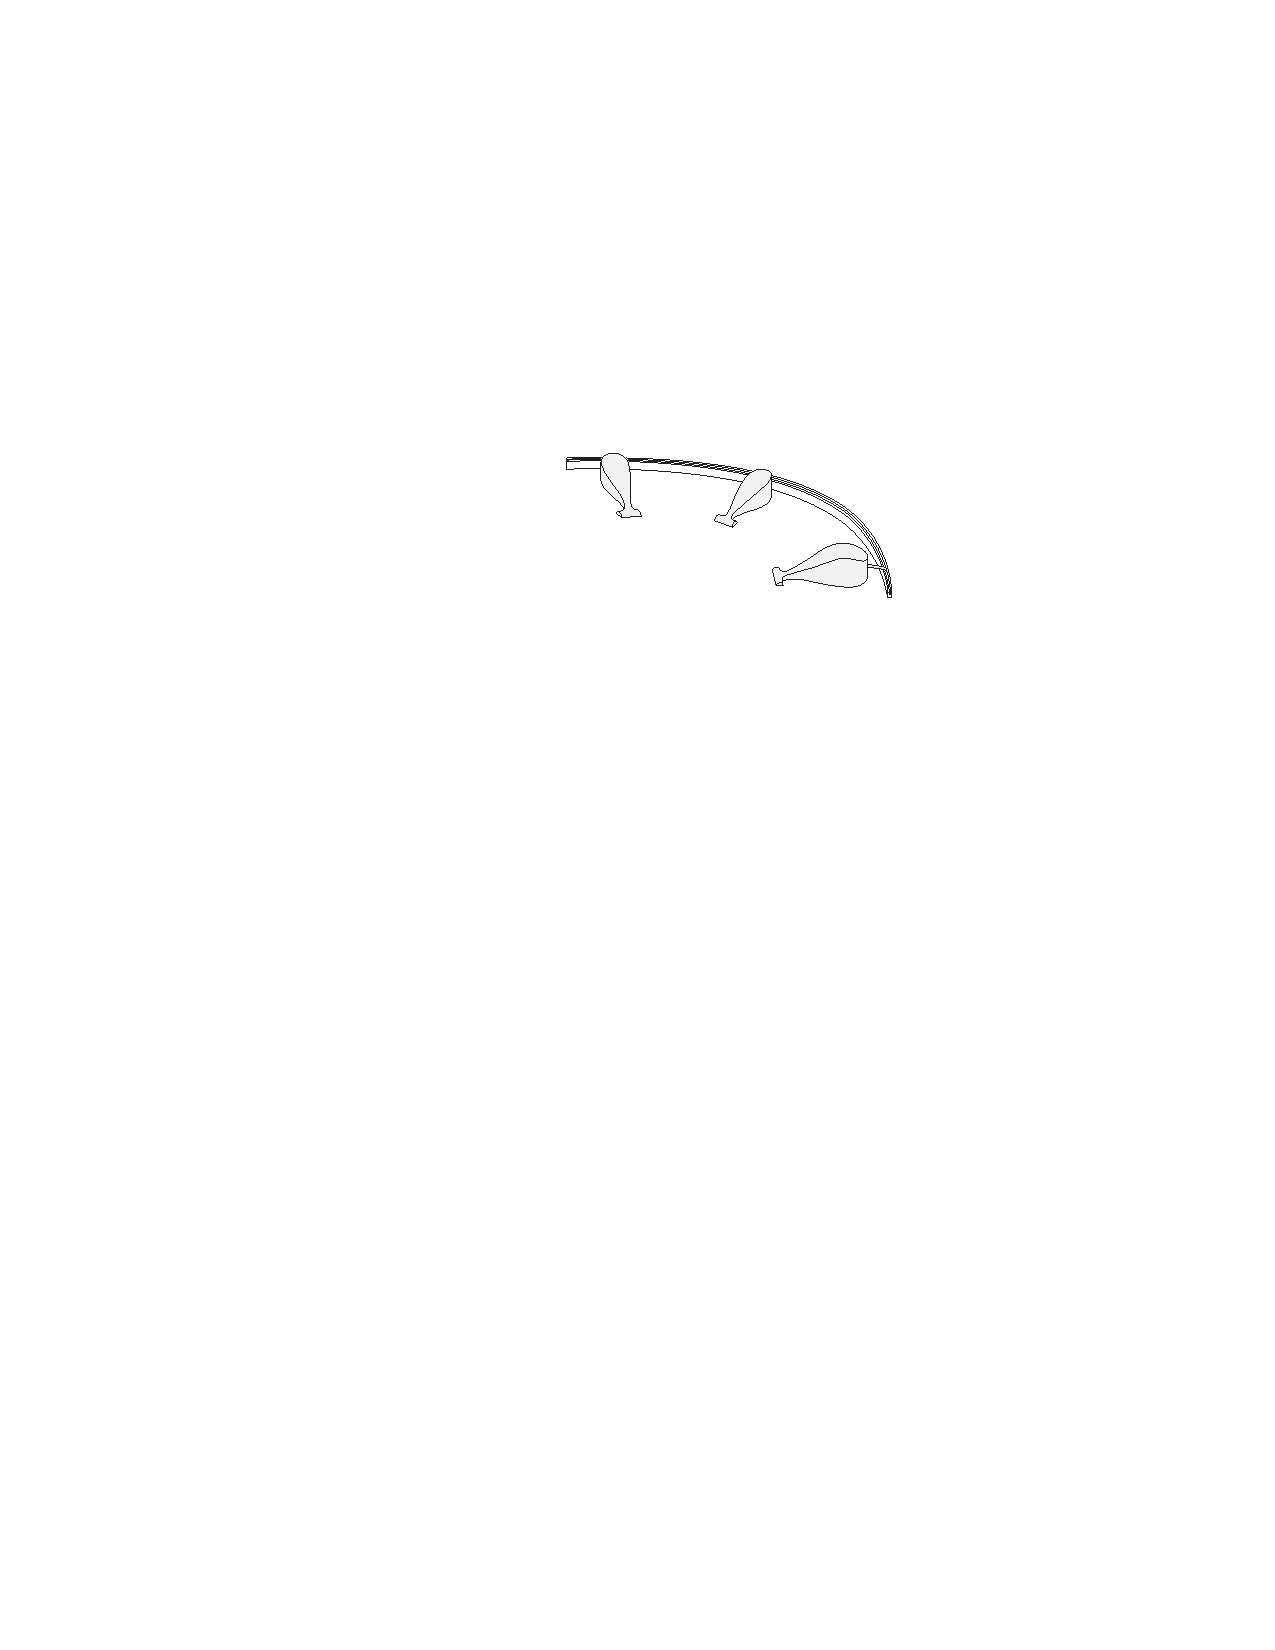
\includegraphics[height=3cm]{Images/Capitulo8/drafting_spline.pdf}
    } \hfill
    \subfloat[\label{fig:inter3}]{
    \begin{tikzpicture}[scale=1.4]
        \draw[-Stealth,thick] (-0.15,0) -- (3,0) node[above left, yshift=2pt] {$x$};
        \draw[-Stealth,thick] (0,-0.15) -- (0,2) node[below right, xshift=2pt] {$y$};
        \draw[gray, domain=0.25:2.9, samples=100] plot(\x,{0.5*(\x - 2)^3 + (\x - 2)^2 + 0.5});
        \filldraw (0.5,{0.5*(0.5 - 2)^3 + (0.5 - 2)^2 + 0.5}) circle (1.5pt);
        \filldraw (0.9,{0.5*(0.9 - 2)^3 + (0.9 - 2)^2 + 0.5}) circle (1.5pt);
        \filldraw (1.3,{0.5*(1.3 - 2)^3 + (1.3 - 2)^2 + 0.5}) circle (1.5pt);
        \filldraw (1.7,{0.5*(1.7 - 2)^3 + (1.7 - 2)^2 + 0.5}) circle (1.5pt);
        \filldraw (2.1,{0.5*(2.1 - 2)^3 + (2.1 - 2)^2 + 0.5}) circle (1.5pt);
        \filldraw (2.5,{0.5*(2.5 - 2)^3 + (2.5 - 2)^2 + 0.5}) circle (1.5pt);
        \filldraw (2.8,{0.5*(2.8 - 2)^3 + (2.8 - 2)^2 + 0.5}) circle (1.5pt);
    \end{tikzpicture}
    }
    \caption{Ejemplos de curvas interpolación}
    \label{fig:enter-label}
\end{figure*}

\section*{Ajuste de curva}

Supongamos que se nos dan $n$ puntos en el plano $xy$,
$$(x_1, y_1), (x_2, y_2), \dots, (x_n, y_n)$$
que deseamos interpolar con una curva “bien comportada” (figura \ref{fig:bienc}). Para mayor comodidad, tomamos los puntos equiespaciados en la dirección $x$, aunque nuestros resultados se pueden extender fácilmente al caso de puntos desigualmente espaciados. Si tomamos la distancia común entre las coordenadas $x$ de los puntos como $h$, entonces tenemos
$$x_2-x_1=x_3-x_2=\cdots=x_n-x_{n-1}=h$$
Sea $y = S(x)$, $x_1 \leq x \leq x_n$, la curva interpolante que buscamos. Suponemos que esta curva describe el desplazamiento de una regla flexible que interpola los $n$ puntos cuando los pesos que sujetan la regla se sitúan precisamente en los $n$ puntos.
\begin{figure}[h!]
    \centering
    \begin{tikzpicture}[
        declare function={
        f(\x) = 0.0125*\x^4 - 0.15*\x^3 + 0.3625*\x^2 + 0.525*\x + 1;
        x1=0;
        x2=1;
        x3=2;
        x4=3;
        x5=4;
        x6=5;
        x7=6;
        }]
        \draw[-Stealth,thick] (-0.15,0) -- (9.25,0) node[above left, yshift=2pt] {$x$};
        \draw[-Stealth,thick] (0,-0.15) -- (0,4) node[below right, xshift=2pt] {$y$};
        \begin{scope}[xshift=1.5cm]
            \draw[gray, domain=0:6, samples=100] plot(\x,{f(\x)});
            \foreach \i in {1,2,3,...,7}
            \filldraw (x\i,{f(x\i)}) circle (1.5pt);
            \foreach \j in {1,2,3,5,6,7}
            \draw[dash pattern=on 3pt off 3pt] (x\j,{f(x\j)}) -- (x\j,0);
            \node at (x7,{f(x7)}) [right] {$(x_n, y_n)$};
            \node at (x6,{f(x6)}) [right] {$(x_{n-1}, y_{n-1})$};
            \node at (x1,{f(x1)}) [left] {$(x_1, y_1)$};
            \node at (x2,{f(x2)}) [left] {$(x_2, y_2)$};
            \node at (x3,{f(x3)}) [left] {$(x_3, y_3)$};
            \foreach \k in {1,2,5,6} {
            \draw[latex-latex] (x\k,0.4) -- (x{\k+1},0.4);
            \node[fill=white,minimum size=0.1mm] at ({0.5*(x\k+x\k+1)},0.4) {$h$};
            }
            \draw[latex-] (3.6,{f(3.6) + 0.05}) -- (4,{f(4) + 0.75}) node[right] {$y = S(x)$};
            \node at (x4,0.4) {$\cdots$};
        \end{scope}
    \end{tikzpicture}
    \caption{~}
    \label{fig:bienc}
\end{figure}

Se sabe, por la teoría de vigas lineales, que para pequeños desplazamientos, la cuarta derivada del desplazamiento de una viga es cero a lo largo de cualquier intervalo del eje $x$ que no contenga fuerzas externas actuando sobre la viga. Si tratamos nuestra regla flexible como una viga delgada y comprendemos que las únicas fuerzas externas actuando sobre ella provienen de los pesos en los $n$ puntos especificados, entonces se sigue que
$$S^{(4)}(x) \equiv 0$$
para valores de $x$ que se encuentran en los $n-1$ intervalos abiertos
$$(x_1, x_2), (x_2, x_3), \dots , (x_{n-1}, x_n)$$
entre los $n$ puntos.

También necesitamos el resultado de la teoría de vigas lineales que establece que, para una viga sujeta únicamente a fuerzas externas, el desplazamiento debe tener dos derivadas continuas. En el caso de la curva interpolante $y = S(x)$ construida con la regla flexible, esto significa que $S(x)$, $S′(x)$ y $S′′(x)$ deben ser continuas para $x_1 \leq x \leq x_n$.

La condición de que $S′′(x)$ sea continua es lo que hace que una regla flexible produzca una curva agradable, ya que resulta en una curvatura continua. El ojo puede percibir cambios bruscos en la curvatura, es decir, discontinuidades en $S′′(x)$, pero los cambios bruscos en derivadas de orden superior no son discernibles. Por lo tanto, la condición de que $S′′(x)$ sea continua es el requisito mínimo para que la curva interpolante sea perceptible como una curva suave única, en lugar de una serie de curvas separadas unidas.

Para determinar la forma matemática de la función $S(x)$, observamos que, dado que $S^{(4)}(x) \equiv 0$ en los intervalos entre los $n$ puntos especificados, se sigue que al resolver esta ecuación repetidamente, $S(x)$ debe ser un polinomio cúbico en $x$ en cada uno de esos intervalos. Sin embargo, en general, $S(x)$ será un polinomio cúbico diferente en cada intervalo, por lo que $S(x)$ debe tener la forma
\begin{equation}
    S(x) = \begin{cases}
        \begin{aligned}
            & S_1(x), & x_1 & \leq x \leq x_2 \\
            & S_2(x), & x_2 & \leq x \leq x_3 \\
            & \phantom{SS} \vdots & & \;\quad \vdots \\
            & S_{n-1}(x), & x_{n-1} & \leq x \leq x_n
        \end{aligned}
    \end{cases} \label{eq:S_interpola}
\end{equation}
donde $S_1(x)$, $S_2(x)$, $\dots$, $S_{n-1}(x)$ son polinomios cúbicos. Para mayor comodidad, los escribiremos de la forma
\begin{align*}
    S_1(x) & = a_1(x - x_1)^3 + b_1(x - x_1)^2 + c_1(x - x_1) + d_1, & x_1 & \leq x \leq x_2 \\
    S_2(x) & = a_2(x - x_2)^3 + b_2(x - x_2)^2 + c_2(x - x_2) + d_2, & x_2 & \leq x \leq x_3 \\
    & \vdots & & \\
    S_{n-1}(x) & = a_{n-1}(x - x_{n-1})^3 + b_{n-1}(x - x_{n-1})^2 & & \\
    & \hspace{3.25cm} + c_{n-1}(x - x_{n-1}) + d_{n-1}, & x_{n-1} & \leq x \leq x_n
\end{align*}
Los $a_i$, $b_i$, $c_i$ y $d_i$ constituyen un total de $4n - 4$ coeficientes que debemos determinar para especificar completamente $S(x)$. Si elegimos estos coeficientes de manera que $S(x)$ interpole los $n$ puntos especificados en el plano y que $S(x)$, $S'(x)$ y $S''(x)$ sean continuos, entonces la curva interpolante resultante se llama \emph{spline cúbico}.

Primero, derivando la expresión \eqref{eq:S_interpola}, es decir, derivando cada polinomio anterior, se sigue que
\begin{align*}
    S'_1(x) & = 3a_1(x - x_1)^2 + 2b_1(x - x_1) + c_1, & x_1 & \leq x \leq x_2 \\
    S'_2(x) & = 3a_2(x - x_2)^2 + 2b_2(x - x_2) + c_2, & x_2 & \leq x \leq x_3 \\
    & \vdots & & \\
    S'_{n-1}(x) & = 3a_{n-1}(x - x_{n-1})^2 + 2b_{n-1}(x - x_{n-1}) + c_{n-1}, & x_{n-1} & \leq x \leq x_n
\end{align*}\newpage\noindent
y derivando nuevamente, obtenemos que
\begin{align*}
    S''_1(x) & = 6a_1(x - x_1) + 2b_1, & x_1 & \leq x \leq x_2 \\
    S''_2(x) & = 6a_2(x - x_2) + 2b_2, & x_2 & \leq x \leq x_3 \\
    & \vdots & & \\
    S''_{n-1}(x) & = 6a_{n-1}(x - x_{n-1}) + 2b_{n-1}, & x_{n-1} & \leq x \leq x_n
\end{align*}
Ahora utilizaremos estas ecuaciones y las cuatro propiedades de los splines cúbicos que se indican a continuación para expresar los coeficientes desconocidos $a_i$, $b_i$, $c_i$, $d_i$ con $i = 1, 2, \dots, n - 1$, en términos de las coordenadas conocidas $y_1$, $y_2$, $\dots$, $y_n$.

\begin{tcolorbox}[
        arc=0mm, 
        bottomtitle=0.5mm,
        boxrule=0mm,
        colbacktitle=black!10!white, 
        coltitle=black,
        left=2.5mm,
        leftrule=1mm,
        right=3.5mm,
        title={$S(x)$ interpola los puntos $(x_i, y_i)$ con $i = 1, 2, \dots, n$.},
        toptitle=0.75mm,
        colframe=black!30!white,
    ]
    Debido a que $S(x)$ interpola los puntos $(x_i, y_i)$, con $i = 1, 2, \dots, n$, tenemos
    \begin{equation}
        S(x_1) = y_1, S(x_2) = y_2, \dots, S(x_n) = y_n \label{YQUJAJAJAJAJJA}
    \end{equation}
    De las primera $n - 1$ de estas ecuaciones y \eqref{eq:S_interpola}, obtenemos
    \begin{equation}
        d_1 = y_1, d_2 = y_2, \dots, d_{n-1} = y_{n-1} \label{UAJAJJAUAUHVCFATQHH}
    \end{equation}
    De la última ecuación en \eqref{YQUJAJAJAJAJJA}, la última ecuación en \eqref{eq:S_interpola}, y el hecho de que $x_n - x_{n-1} = h$, obtenemos
    \begin{equation}
        a_{n-1}h^3 + b_{n-1}h^2 + c_{n-1}h + d_{n-1} = y_n \label{UAJAJAHHCCFGYYQUYQHUU}
    \end{equation}
\end{tcolorbox}

\begin{tcolorbox}[
        arc=0mm, 
        bottomtitle=0.5mm,
        boxrule=0mm,
        colbacktitle=black!10!white, 
        coltitle=black,
        left=2.5mm,
        leftrule=1mm,
        right=3.5mm,
        title={$S(x)$ es continua en $[x_1, x_n]$.},
        toptitle=0.75mm,
        colframe=black!30!white,
    ]
    Debido a que $S(x)$ es continuo para $x_1 \leq x \leq x_n$, se deduce que en cada punto $x_i$ en el conjunto $x_2$, $x_3$, $\dots$, $x_{n-1}$ debemos tener
    \begin{equation}
        S_{i-1}(x_i) = S_i(x_i), \quad i = 2, 3, \dots, n-1 \label{JAJAJAJJAJAVHHGGGQ}
    \end{equation}
    De lo contrario, las gráficas de $S_{i-1}(x)$ y $S_i(x)$ no se unirían para formar una curva continua en $x_i$. Cuando aplicamos la propiedad de interpolación $S_i(x_i) = y_i$, se sigue de \eqref{JAJAJAJJAJAVHHGGGQ} que $S_{i-1}(x_i) = y_i$ donde $i = 2, 3, \dots, n-1$, o de \eqref{eq:S_interpola} que
    \begin{equation}
        \begin{aligned}
            a_1h^3 + b_1h^2 + c_1h + d_1 & = y_2 \\
            a_2h^3 + b_2h^2 + c_2h + d_2 & = y_3 \\
            & \vdots \\
            a_{n-2}h^3 + b_{n-2}h^2 + c_{n-2}h + d_{n-2} & = y_{n-1}
        \end{aligned} \label{UAUAJAHCCGTTQRTQHCCTAT}
    \end{equation}
\end{tcolorbox}

\begin{tcolorbox}[
        arc=0mm, 
        bottomtitle=0.5mm,
        boxrule=0mm,
        colbacktitle=black!10!white, 
        coltitle=black,
        left=2.5mm,
        leftrule=1mm,
        right=3.5mm,
        title={$S'(x)$ es continua en $[x_1, x_n]$.},
        toptitle=0.75mm,
        colframe=black!30!white,
    ]
    Debido a que $S'(x)$ es continuo para $x_1 \leq x \leq x_n$, se deduce que
    $$S'_{i-1}(x_i) = S'_i(x_i), \quad i = 2, 3, \dots, n-1$$
    es decir
    \begin{equation}
        \begin{aligned}
            3a_1h^2 + 2b_1h + c_1 & = c_2 \\
            3a_2h^2 + 2b_2h + c_2 & = c_3 \\
            & \vdots \\
            3a_{n-2}h^2 + 2b_{n-2}h + c_{n-2} & = c_{n-1}
        \end{aligned} \label{HAJAHAHCCFGYYYAGQTTQYQHHA}
    \end{equation}
\end{tcolorbox}

\newpage

\begin{tcolorbox}[
        arc=0mm, 
        bottomtitle=0.5mm,
        boxrule=0mm,
        colbacktitle=black!10!white, 
        coltitle=black,
        left=2.5mm,
        leftrule=1mm,
        right=3.5mm,
        title={$S''(x)$ es continua en $[x_1, x_n]$.},
        toptitle=0.75mm,
        colframe=black!30!white,
    ]
    Debido a que $S''(x)$ es continuo para $x_1 \leq x \leq x_n$, se deduce que
    $$S''_{i-1}(x_i) = S''_i(x_i), \quad i = 2, 3, \dots, n-1$$
    es decir
    \begin{equation}
        \begin{aligned}
            6a_1h + 2b_1 & = 2b_2 \\
            6a_2h + 2b_2 & = 2b_3 \\
            & \vdots \\
            6a_{n-2}h + 2b_{n-2} & = 2b_{n-1}
        \end{aligned} \label{YAYACCXFTQTRQRTQZFGTA}
    \end{equation}
\end{tcolorbox}

Las ecuaciones \eqref{UAJAJJAUAUHVCFATQHH}, \eqref{UAJAJAHHCCFGYYQUYQHUU}, \eqref{UAUAJAHCCGTTQRTQHCCTAT}, \eqref{HAJAHAHCCFGYYYAGQTTQYQHHA} y \eqref{YAYACCXFTQTRQRTQZFGTA} constituyen un sistema de $4n - 6$ ecuaciones lineales con $4n - 4$ coeficientes desconocidos $a_i$, $b_i$, $c_i$, $d_i$ con $i = 1, 2, \dots, n-1$. Por lo tanto, necesitamos dos ecuaciones más para determinar estos coeficientes de manera única. Sin embargo, antes de obtener estas ecuaciones adicionales, podemos simplificar nuestro sistema existente expresando las incógnitas $a_i$, $b_i$, $c_i$ y $d_i$ en términos de nuevas cantidades desconocidas:
$$M_1 = S''(x_1), M_2 = S''(x_2), \dots, M_n = S''(x_n)$$
y las cantidades conocidas $y_1$, $y_2$, $\dots$, $y_n$. Es decir,
\begin{align*}
    M_1 & = 2b_1 \\
    M_2 & = 2b_2 \\
    & \vdots \\
    M_{n-1} & = 2b_{n-1}
\end{align*}
así que
$$b_1 = \frac{1}{2}M_1, b_2 = \frac{1}{2}M_2, \dots, b_{n-1} = \frac{1}{2}M_{n-1}$$
Además, sabemos de \eqref{UAJAJJAUAUHVCFATQHH} que
$$d_1 = y_1, d_2 = y_2, \dots, d_{n-1} = y_{n-1}$$
Dejamos como ejercicio al lector derivar las expresiones de los $a_i$ y $c_i$ en términos de los $M_i$ y $y_i$. El resultado final es el siguiente:
\begin{theorem}[Interpolación mediante splines cúbicos]
    Dados $n$ puntos $(x_1, y_1)$, $(x_2, y_2)$, $\dots$, $(x_n, y_n)$ con $x_{i+1} - x_i = h$ e $i = 1, 2, \dots, n - 1$, el spline cúbico
    $$S(x) = \begin{cases}
        \begin{aligned}
            & a_1(x - x_1)^3 + b_1(x - x_1)^2 + c_1(x - x_1) + d_1, & x_1 & \leq x \leq x_2 \\
            & a_2(x - x_2)^3 + b_2(x - x_2)^2 + c_2(x - x_2) + d_2, & x_2 & \leq x \leq x_3 \\
            & \hspace{3cm} \vdots & & \\
            & a_{n-1}(x - x_{n-1})^3 + b_{n-1}(x - x_{n-1})^2 & & \\
            & \hspace{2.75cm} + c_{n-1}(x - x_{n-1}) + d_{n-1}, & x_{n-1} & \leq x \leq x_n
        \end{aligned}
    \end{cases}$$
    que interpola estos puntos tiene como coeficientes a
    \begin{equation}
        \begin{aligned}
            a_i & = \frac{M_{i+1} - M_i}{6h} \\
            b_i & = \frac{M_i}{2} \\
            c_i & = \frac{y_{i+1} - y_i}{h} - \frac{(M_{i+1} + 2M_i)h}{6} \\
            d_i & = y_i
        \end{aligned} \label{JAJAJAIIQIQUQJAHHAVGH}
    \end{equation}
    para $i = 1, 2, \dots, n - 1$, donde $M_i = S''(x_i)$ con $i = 1, 2, \dots, n$.
\end{theorem}

\newpage

A partir de este resultado, vemos que las cantidades $M_1$, $M_2$, $\dots$, $M_n$ determinan de manera única el spline cúbico. Para encontrar estas cantidades, sustituimos las expresiones de $a_i$, $b_i$ y $c_i$ dadas en \eqref{JAJAJAIIQIQUQJAHHAVGH} en \eqref{HAJAHAHCCFGYYYAGQTTQYQHHA}. Después de algunas simplificaciones algebraicas, obtenemos
\begin{equation}
    \begin{aligned}
        M_1 + 4M_2 + M_3 & = \frac{6(y_1 - 2y_2 + y_3)}{h^2} \\
        M_2 + 4M_3 + M_4 & = \frac{6(y_2 - 2y_3 + y_4)}{h^2} \\
        & \vdots \\
        M_{n-2} + 4M_{n-1} + M_n & = \frac{6(y_{n-2} - 2y_{n-1} + y_n)}{h^2}
    \end{aligned} \label{JAJAHAGYATTQTTFFFQTTTTQ}
\end{equation}
o, en forma matricial,
$$\begin{bmatrix}
    1 & 4 & 1 & 0 & \cdots & 0 & 0 & 0 & 0 \\
    0 & 1 & 4 & 1 & \cdots & 0 & 0 & 0 & 0 \\
    0 & 0 & 1 & 4 & \cdots & 0 & 0 & 0 & 0 \\
    \vdots & \vdots & & \ddots & \ddots & \ddots & & \vdots & \vdots \\
    0 & 0 & 0 & 0 & \cdots & 4 & 1 & 0 & 0 \\
    0 & 0 & 0 & 0 & \cdots & 1 & 4 & 1 & 0 \\
    0 & 0 & 0 & 0 & \cdots & 0 & 1 & 4 & 1
\end{bmatrix} \begin{bmatrix}
    M_1 \\
    M_2 \\
    M_3 \\
    \vdots \\
    M_{n-2} \\
    M_{n-1} \\
    M_n
\end{bmatrix} = \frac{6}{h^2} \begin{bmatrix}
    y_1 - 2y_2 + y_3 \\
    y_2 - 2y_3 + y_4 \\
    y_3 - 2y_4 + y_5 \\
    \vdots \\
    y_{n-4} - 2y_{n-3} + y_{n-2} \\
    y_{n-3} - 2y_{n-2} + y_{n-1} \\
    y_{n-2} - 2y_{n-1} + y_n
\end{bmatrix}$$
Observemos que este es un sistema lineal de $n - 2$ ecuaciones con $n$ incógnitas dadas por $M_1$, $M_2$, $\dots$, $M_n$. Por lo tanto, todavía necesitamos dos ecuaciones adicionales para determinar $M_1$, $M_2$, $\dots$, $M_n$ de manera única. La razón de esto es que hay infinitos splines cúbicos que interpolan los puntos dados, por lo que simplemente no tenemos suficientes condiciones para determinar un spline cúbico único que pase por los puntos. A continuación, discutiremos tres posibles formas de especificar las dos condiciones adicionales requeridas para obtener un spline cúbico único a través de los puntos. Esto puede resumirse como se muestra en la siguiente tabla:
\begin{table*}[h!]
    \centering
    \begin{NiceTabular}{ccc}[hvlines,cell-space-limits=4pt]
        \cellcolor{black!20!white}{\makecell{Spline \\ natural}} & $\begin{aligned} M_1 & = 0 \\ M_n & = 0 \end{aligned}$ & $\begin{bmatrix} 4 & 1 & 0 & \cdots & 0 & 0 & 0 \\ 1 & 4 & 1 & \cdots & 0 & 0 & 0 \\ \vdots & & \ddots & \ddots & \ddots & & \vdots \\ 0 & 0 & 0 & \cdots & 1 & 4 & 1 \\ 0 & 0 & 0 & \cdots & 0 & 1 & 4 \end{bmatrix} \begin{bmatrix} M_2 \\ M_3 \\ \vdots \\ M_{n-2} \\ M_{n-1} \end{bmatrix} = \dfrac{6}{h^2} \begin{bmatrix} y_1 - 2y_2 + y_3 \\ y_2 - 2y_3 + y_4 \\ \vdots \\ y_{n-3} - 2y_{n-2} + y_{n-1} \\ y_{n-2} - 2y_{n-1} + y_n \end{bmatrix}$ \\
        \cellcolor{black!20!white}{\makecell{Spline de \\ salida \\ parabólica}} & $\begin{aligned} M_1 & = M_2 \\ M_n & = M_{n-1} \end{aligned}$ & $\begin{bmatrix} 5 & 1 & 0 & \cdots & 0 & 0 & 0 \\ 1 & 4 & 1 & \cdots & 0 & 0 & 0 \\ \vdots & & \ddots & \ddots & \ddots & & \vdots \\ 0 & 0 & 0 & \cdots & 1 & 4 & 1 \\ 0 & 0 & 0 & \cdots & 0 & 1 & 5 \end{bmatrix} \begin{bmatrix} M_2 \\ M_3 \\ \vdots \\ M_{n-2} \\ M_{n-1} \end{bmatrix} = \dfrac{6}{h^2} \begin{bmatrix} y_1 - 2y_2 + y_3 \\ y_2 - 2y_3 + y_4 \\ \vdots \\ y_{n-3} - 2y_{n-2} + y_{n-1} \\ y_{n-2} - 2y_{n-1} + y_n \end{bmatrix}$ \\
        \cellcolor{black!20!white}{\makecell{Spline de \\ salida \\ cúbica}} & $\begin{aligned} M_1 & = 2M_2 - M_3 \\ M_n & = 2M_{n-1} - M_{n-2} \end{aligned}$ & $\begin{bmatrix} 6 & 0 & 0 & \cdots & 0 & 0 & 0 \\ 1 & 4 & 1 & \cdots & 0 & 0 & 0 \\ \vdots & & \ddots & \ddots & \ddots & & \vdots \\ 0 & 0 & 0 & \cdots & 1 & 4 & 1 \\ 0 & 0 & 0 & \cdots & 0 & 0 & 6 \end{bmatrix} \begin{bmatrix} M_2 \\ M_3 \\ \vdots \\ M_{n-2} \\ M_{n-1} \end{bmatrix} = \dfrac{6}{h^2} \begin{bmatrix} y_1 - 2y_2 + y_3 \\ y_2 - 2y_3 + y_4 \\ \vdots \\ y_{n-3} - 2y_{n-2} + y_{n-1} \\ y_{n-2} - 2y_{n-1} + y_n \end{bmatrix}$
    \end{NiceTabular}
\end{table*}\vspace{-0.5cm}

\noindent Es decir,
\begin{itemize}
    \item Spline natural: La segunda derivada del spline es cero en los extremos.
    \item Spline de salida parabólica: El spline se reduce a una curva parabólica en los primeros y últimos intervalos.
    \item Spline de salida cúbica: El spline es una única curva cúbica en los dos primeros y los dos últimos intervalos.
\end{itemize}

\newpage

\subsection*{El spline natural}

Las dos condiciones matemáticas más simples que podemos imponer son
$$M_1 = M_n = 0$$
Estas condiciones, junto con \eqref{JAJAHAGYATTQTTFFFQTTTTQ}, resultan en un sistema lineal de $n \times n$ para $M_1$, $M_2$, $\dots$, $M_n$, que se puede escribir en forma matricial como
$$\begin{bmatrix}
    1 & 0 & 0 & 0 & \cdots & 0 & 0 & 0 \\
    1 & 4 & 1 & 0 & \cdots & 0 & 0 & 0 \\
    0 & 1 & 4 & 1 & \cdots & 0 & 0 & 0 \\
    \vdots & \vdots & & \ddots & \ddots & \ddots & & \vdots \\
    0 & 0 & 0 & 0 & \cdots & 1 & 4 & 1 \\
    0 & 0 & 0 & 0 & \cdots & 0 & 0 & 1
\end{bmatrix} \begin{bmatrix}
    M_1 \\
    M_2 \\
    M_3 \\
    \vdots \\
    M_{n-1} \\
    M_n
\end{bmatrix} = \frac{6}{h^2} \begin{bmatrix}
    0 \\
    y_2 - 2y_3 + y_4 \\
    y_3 - 2y_4 + y_5 \\
    \vdots \\
    y_{n-2} - 2y_{n-1} + y_n \\
    0
\end{bmatrix}$$
Para cálculos numéricos, es más conveniente eliminar $M_1$ y $M_n$ de este sistema y escribir
$$\begin{bmatrix}
    4 & 1 & 0 & 0 & \cdots & 0 & 0 & 0 \\
    1 & 4 & 1 & 0 & \cdots & 0 & 0 & 0 \\
    0 & 1 & 4 & 1 & \cdots & 0 & 0 & 0 \\
    \vdots & \vdots & & \ddots & \ddots & \ddots & & \vdots \\
    0 & 0 & 0 & 0 & \cdots & 1 & 4 & 1 \\
    0 & 0 & 0 & 0 & \cdots & 0 & 1 & 4
\end{bmatrix} \begin{bmatrix}
    M_2 \\
    M_3 \\
    M_4 \\
    \vdots \\
    M_{n-2} \\
    M_{n-1}
\end{bmatrix} = \frac{6}{h^2} \begin{bmatrix}
    y_1 - 2y_2 + y_3 \\
    y_2 - 2y_3 + y_4 \\
    y_3 - 2y_4 + y_5 \\
    \vdots \\
    y_{n-3} - 2y_{n-2} + y_{n-1} \\
    y_{n-2} - 2y_{n-1} + y_n
\end{bmatrix}$$
junto con
\begin{align}
    M_1 & = 0 \label{UAJAJAJUAHGGGQGQGA} \\
    M_2 & = 0 \label{JAJJAJAJAJABSJSIPP}
\end{align}
Así, el sistema lineal de $(n - 2) \times (n - 2)$ puede resolverse para los $n - 2$ coeficientes $M_2$, $M_3$, $\dots$, $M_{n-1}$, y $M_1$ y $M_n$ están determinados mediante \eqref{UAJAJAJUAHGGGQGQGA} y \eqref{JAJJAJAJAJABSJSIPP}.

Físicamente, el spline natural resulta cuando los extremos de una regla flexible se extienden libremente más allá de los puntos interpolados sin restricción. Las porciones finales del spline fuera de los puntos interpolados caerán en trayectorias de líneas rectas, lo que hace que $S''(x)$ se anule en los extremos $x_1$ y $x_n$, y resultando en las condiciones matemáticas $M_1 = M_n = 0$.

El spline natural tiende a aplanar la curva interpolante en los extremos, lo cual puede ser indeseable. Por supuesto, si se requiere que $S''(x)$ se anule en los extremos, entonces se debe usar el spline natural.

\subsection*{El spline de salida parabólica}

Las dos restricciones adicionales impuestas para este tipo de spline son
\begin{align}
    M_1 & = M_2 \label{UAUAJAJJAJAVAHAGQVAHAH} \\
    M_n & = M_{n-1} \label{JAJAJAUAUJAYAYQYQHGAJ}
\end{align}
Si utilizamos las dos ecuaciones anteriores para eliminar $M_1$ y $M_n$ de \eqref{JAJAHAGYATTQTTFFFQTTTTQ}, obtenemos el sistema lineal de $(n - 2) \times (n - 2)$
$$\begin{bmatrix}
    5 & 1 & 0 & 0 & \cdots & 0 & 0 & 0 \\
    1 & 4 & 1 & 0 & \cdots & 0 & 0 & 0 \\
    0 & 1 & 4 & 1 & \cdots & 0 & 0 & 0 \\
    \vdots & \vdots & & \ddots & \ddots & \ddots & & \vdots \\
    0 & 0 & 0 & 0 & \cdots & 1 & 4 & 1 \\
    0 & 0 & 0 & 0 & \cdots & 0 & 1 & 5
\end{bmatrix} \begin{bmatrix}
    M_2 \\
    M_3 \\
    M_4 \\
    \vdots \\
    M_{n-2} \\
    M_{n-1}
\end{bmatrix} = \frac{6}{h^2} \begin{bmatrix}
    y_1 - 2y_2 + y_3 \\
    y_2 - 2y_3 + y_4 \\
    y_3 - 2y_4 + y_5 \\
    \vdots \\
    y_{n-3} - 2y_{n-2} + y_{n-1} \\
    y_{n-2} - 2y_{n-1} + y_n
\end{bmatrix}$$\newpage\noindent

para $M_2$, $M_3$, $\dots$, $M_{n-1}$. Una vez que se han determinado estos $n - 2$ valores, $M_1$ y $M_n$ se determinan a partir de \eqref{UAUAJAJJAJAVAHAGQVAHAH} y \eqref{JAJAJAUAUJAYAYQYQHGAJ}.

De \eqref{JAJAJAIIQIQUQJAHHAVGH} observemos que $M_1 = M_2$ implica que $a_1 = 0$, y $M_n = M_{n-1}$ implica que $a_{n-1} = 0$. Por lo tanto, en \eqref{eq:S_interpola} no hay términos cúbicos para el spline sobre los intervalos $[x_1, x_2]$ y $[x_{n-1}, x_n]$. Por lo tanto, como sugiere el nombre, el spline de salida parabólica se reduce a una curva parabólica sobre estos intervalos finales.

\subsection*{El spline de salida cúbica}

Para este tipo de spline, imponemos las siguientes dos condiciones adicionales
\begin{align}
    M_1 & = 2M_2 - M_3 \label{JAJAJJAJAJQJQHCVAHAJ} \\
    M_n & = 2M_{n-1} - M_2 \label{JAJAJAJJAJAAJJAJABAJ}
\end{align}
Usando estas dos ecuaciones para eliminar $M_1$ y $M_n$ de \eqref{JAJAHAGYATTQTTFFFQTTTTQ}, resulta en el siguiente sistema lineal de $(n - 2) \times (n - 2)$ para $M_2$, $M_3$, $\dots$, $M_{n-1}$:
$$\begin{bmatrix}
    6 & 0 & 0 & 0 & \cdots & 0 & 0 & 0 \\
    1 & 4 & 1 & 0 & \cdots & 0 & 0 & 0 \\
    0 & 1 & 4 & 1 & \cdots & 0 & 0 & 0 \\
    \vdots & \vdots & & \ddots & \ddots & \ddots & & \vdots \\
    0 & 0 & 0 & 0 & \cdots & 1 & 4 & 1 \\
    0 & 0 & 0 & 0 & \cdots & 0 & 1 & 6
\end{bmatrix} \begin{bmatrix}
    M_2 \\
    M_3 \\
    M_4 \\
    \vdots \\
    M_{n-2} \\
    M_{n-1}
\end{bmatrix} = \frac{6}{h^2} \begin{bmatrix}
    y_1 - 2y_2 + y_3 \\
    y_2 - 2y_3 + y_4 \\
    y_3 - 2y_4 + y_5 \\
    \vdots \\
    y_{n-3} - 2y_{n-2} + y_{n-1} \\
    y_{n-2} - 2y_{n-1} + y_n
\end{bmatrix}$$
Después de resolver este sistema lineal para $M_2$, $M_3$, $\dots$, $M_{n-1}$, podemos usar \eqref{JAJAJJAJAJQJQHCVAHAJ} y \eqref{JAJAJAJJAJAAJJAJABAJ} para determinar $M_1$ y $M_n$.

Si reescribimos \eqref{JAJAJJAJAJQJQHCVAHAJ} como
$$M_2 - M_1 = M_3 - M_2$$
se sigue de \eqref{JAJAJAIIQIQUQJAHHAVGH} que $a_1 = a_2$ y debido a que $S'''(x) = 6a_1$ en $[x_1, x_2]$ y $S'''(x) = 6a_2$ en $[x_2, x_3]$, vemos que $S'''(x)$ es constante sobre todo el intervalo $[x_1, x_3]$. En consecuencia, $S(x)$ consiste en una única curva cúbica sobre el intervalo $[x_1, x_3]$ en lugar de dos curvas cúbicas diferentes unidas en $x_2$. Un análisis similar muestra que $S(x)$ consiste en una única curva cúbica sobre los últimos dos intervalos.

Mientras que el spline natural tiende a producir una curva interpolante que es plana en los extremos, el spline de terminación cúbica tiene la tendencia opuesta: produce una curva con curvatura pronunciada en los extremos. Si ninguno de estos comportamientos es deseado, el spline de terminación parabólica ofrece una alternativa equilibrada.

\begin{example}
    La densidad del agua se sabe que alcanza un máximo a una temperatura ligeramente superior al punto de congelación. La siguiente tabla proporciona la densidad del agua en gramos por centímetro cúbico para cinco temperaturas igualmente espaciadas desde $-10$º$\mathrm{C}$ hasta $30$º$\mathrm{C}$.
    \begin{table}[h!]
        \centering
        \begin{NiceTabular}{ccc}[hvlines,cell-space-limits=3pt]
            \cellcolor{black!20!white}{Temperatura (º$\mathrm{C}$)} & \cellcolor{black!20!white}{Densidad ($\mathrm{g}/\mathrm{cm}^3$)} \\
            \makecell[r]{$-10$ \\ $0$ \\ $10$ \\ $20$ \\ $30$} & \makecell[r]{$0.99815$ \\ $0.99987$ \\ $0.99973$ \\ $0.99823$ \\ $0.99567$}
        \end{NiceTabular}
    \end{table}\newpage\noindent
    Vamos a interpolar estas cinco mediciones de temperatura-densidad con un spline de salida parabólica y trataremos de encontrar la densidad máxima del agua en este rango hallando el valor máximo en este spline cúbico. Sean
    \begin{align*}
        x_1 & = -10 & y_1 & = 0.99815 \\
        x_2 & = 0 & y_2 & = 0.99987 \\
        x_3 & = 10 & y_3 & = 0.99973 \\
        x_4 & = 20 & y_4 & = 0.99823 \\
        x_5 & = 30 & y_5 & = 0.99567
    \end{align*}
    entonces
    \begin{align*}
        \frac{6(y_1 - 2y_2 + y_3)}{h^2} & = \frac{6\big(0.99815 - 2(0.99987) + 0.99973\big)}{10^2} = -0.0001116 \\
        \frac{6(y_2 - 2y_3 + y_4)}{h^2} & = \frac{6\big(0.99987 - 2(0.99973) + 0.99823\big)}{10^2} = -0.0000816 \\
        \frac{6(y_3 - 2y_4 + y_5)}{h^2} & = \frac{6\big(0.99973 - 2(0.99823) + 0.99567\big)}{10^2} = -0.0000636
    \end{align*}
    y el sistema lineal para el spline de salida parabólica se convierte en
    $$\begin{bmatrix}
        5 & 1 & 4 \\
        1 & 4 & 1 \\
        0 & 1 & 5
    \end{bmatrix} \begin{bmatrix}
        M_2 \\
        M_3 \\
        M_4
    \end{bmatrix} = \begin{bmatrix*}[r]
        -0.0001116 \\
        -0.0000816 \\
        -0.0000636
    \end{bmatrix*}$$
    Al resolver este sistema, da como resultado
    $$M_2 = -0.00001973, \qquad M_3 = -0.00001293, \qquad M_4 = -0.00001013$$
    De \eqref{UAUAJAJJAJAVAHAGQVAHAH} y \eqref{JAJAJAUAUJAYAYQYQHGAJ}, tenemos que
    \begin{align*}
        M_1 & = M_2 = -0.00001973 \\
        M_5 & = M_4 = -0.00001013
    \end{align*}
    Al resolver para los $a_i$, $b_i$, $c_i$ y $d_i$ en \eqref{JAJAHAGYATTQTTFFFQTTTTQ}, obtenemos la siguiente expresión para el spline de terminación parabólica interpolante:
    $$S(x) = \begin{cases}
        \begin{aligned}
            -0.00000987(x + 10)^2 + 0.002707(x + 10) + 0.99815, & & -10 & \leq x \leq 0 \\
            0.00000113(x - 0)^3 - 0.00000987(x - 0)^2 + 0.000733(x - 0) + 0.99987, & & 0 & \leq x \leq 10 \\
            0.00000047(x - 10)^3 - 0.00000647(x - 10)^2 - 0.000900(x - 10) + 0.99973, & & 10 & \leq x \leq 20 \\
            - 0.00000507(x - 20)^2 - 0.002053(x - 20) + 0.99823, & & 10 & \leq x \leq 20
        \end{aligned}
    \end{cases}$$
    Este spline se muestra en la siguiente figura:
    \begin{center}
        \begin{tikzpicture}
            \draw (0,0) grid (4,5);
            \foreach \i in {-1,1,2,3}
            \node[below] at (\i+1,0) {$\i 0$};
            \node[below] at (1,0) {$0$};
            \foreach \j in {5,6,7,8,9}
            \node[left] at (0,\j-5) {$0.99 \j 00$};
            \node[left] at (0,5) {$1.00000$};
            \draw[gray, domain=0:4, samples=100] plot(\x,{-0.0166666666667*\x^4 + 0.25*\x^3 - 1.683333333333*\x^2 + 3.25*\x + 3.1});
            \filldraw (0,3.1) circle (1.5pt);
            \filldraw (1,4.9) circle (1.5pt);
            \filldraw (2,4.6) circle (1.5pt);
            \filldraw (3,3.12) circle (1.5pt);
            \filldraw (4,0.9) circle (1.5pt);
            \node at (2,-0.75) {Temperatura (º$\mathrm{C}$)};
            \node[rotate=90] at (-1.75,2.5) {Densidad ($\mathrm{g}/\mathrm{cm}^3$)};
        \end{tikzpicture}
    \end{center}\newpage\noindent
    En dicha figura, vemos que el máximo se alcanza en el intervalo $[0, 10]$. Para encontrar este máximo, igualamos $S'(x)$ a cero en el intervalo $[0, 10]$:
    $$S'(x) = 0.000000339x^2 - 0.0001974x + 0.0000733 = 0$$
    Con tres cifras significativas, la raíz de esta ecuación cuadrática en el intervalo $[0, 10]$ es $x = 3.99$, y para este valor de $x$, $S(3.99) = 1.00001$. Así, según nuestra estimación interpolada, la densidad máxima del agua es $1.00001$ $\mathrm{g}/\mathrm{cm}^3$ alcanzada a $3.99$º$\mathrm{C}$. Esto concuerda bien con la densidad máxima experimental de $1.00000$ $\mathrm{g}/\mathrm{cm}^3$ alcanzada a $3.98$º$\mathrm{C}$.
\end{example}

En conclusión, además de producir excelentes curvas de interpolación, los splines cúbicos y sus generalizaciones son útiles para la integración y diferenciación numérica, para la solución numérica de ecuaciones diferenciales e integrales, y en la teoría de la optimización.

\section{Cadenas de Markov}

Supongamos que un sistema físico o matemático atraviesa un proceso de cambio de tal manera que en cualquier momento puede ocupar uno de un número finito de estados. Por ejemplo, el clima en una ciudad determinada podría estar en uno de tres posibles estados: soleado, nublado o lluvioso. O imaginemos que un individuo podría estar en uno de cuatro posibles estados emocionales: feliz, triste, enojado o aprensivo. Supongamos que tal sistema cambia con el tiempo de un estado a otro y que en momentos programados se observa el estado del sistema. Si el estado del sistema en una observación no puede predecirse con certeza, pero la probabilidad de que ocurra un estado dado puede predecirse simplemente conociendo el estado del sistema en la observación precedente, entonces el proceso de cambio se llama \emph{cadena de Markov} o \emph{proceso de Markov}.

\begin{definition}
    Si una cadena de Markov tiene $k$ posibles estados, etiquetados como $1, 2, \ldots, k$, entonces la probabilidad de que el sistema esté en el estado $i$ en una observación, después de haber estado en el estado $j$ en la observación anterior, se denota por $p_{ij}$ y se llama probabilidad de transición del estado $j$ al estado $i$. La matriz $P = \llparenthesis p_{ij} \rrparenthesis$ se llama \emph{matriz de transición de la cadena de Markov}.
\end{definition}

Por ejemplo, en una cadena de Markov de tres estados, la matriz de transición tiene la forma\\
\begin{nscenter}
    \begin{tikzpicture}
        \node (A) at (0,0) {$\begin{bmatrix} p_{11} & p_{12} & p_{13} \\ p_{21} & p_{22} & p_{23} \\ p_{31} & p_{32} & p_{33} \end{bmatrix}$};
        \node[black!90!white, xshift=-0.85cm, yshift=0.1cm] at (A.north) {$1$};
        \node[black!90!white, yshift=0.1cm] at (A.north) {$2$};
        \node[black!90!white, xshift=0.85cm, yshift=0.1cm] at (A.north) {$3$};
        \node[black!90!white,yshift=0.4cm] at (A.east) {$1$};
        \node[black!90!white] at (A.east) {$2$};
        \node[black!90!white,yshift=-0.4cm] at (A.east) {$3$};
        \node[yshift=0.75cm] at (A.north) {Estado precedente};
        \node[right,xshift=0.5cm] at (A.east) {Nuevo estado};
    \end{tikzpicture}
\end{nscenter}
En esta matriz, $p_{32}$ es la probabilidad de que el sistema cambie del estado $2$ al estado $3$, $p_{11}$ es la probabilidad de que el sistema permanezca en el estado $1$ si estaba previamente en el estado $1$, y así sucesivamente.

\begin{example}\label{exam:markov1}
    Una agencia de alquiler de coches tiene tres ubicaciones de alquiler, denominadas $1$, $2$ y $3$. Un cliente puede alquilar un coche en cualquiera de las tres ubicaciones y devolverlo a cualquiera de las tres ubicaciones. El gerente encuentra que los clientes devuelven los coches a las diversas ubicaciones según las siguientes probabilidades:\newpage
    \begin{nscenter}
        \begin{tikzpicture}
            \node (A) at (0,0) {$\begin{bmatrix} 0.8 & 0.3 & 0.2 \\ 0.1 & 0.2 & 0.6 \\ 0.1 & 0.5 & 0.2 \end{bmatrix}$};
            \node[black!90!white, xshift=-0.85cm, yshift=0.1cm] at (A.north) {$1$};
            \node[black!90!white, yshift=0.1cm] at (A.north) {$2$};
            \node[black!90!white, xshift=0.85cm, yshift=0.1cm] at (A.north) {$3$};
            \node[black!90!white,yshift=0.4cm] at (A.east) {$1$};
            \node[black!90!white] at (A.east) {$2$};
            \node[black!90!white, yshift=-0.4cm] at (A.east) {$3$};
            \node[yshift=0.75cm] at (A.north) {Alquilado desde la ubicación};
            \node[right,xshift=0.5cm] at (A.east) {\makecell{Regresado \\ a la \\ ubicación}};
        \end{tikzpicture}
    \end{nscenter}
    Esta matriz es la matriz de transición del sistema considerado como una cadena de Markov. De esta matriz, se puede ver que la probabilidad de que un coche alquilado en la ubicación $3$ sea devuelto a la ubicación $2$ es de $0.3$, la probabilidad de que un coche alquilado en la ubicación $1$ sea devuelto a la ubicación $1$ es de $0.5$, y así sucesivamente.
\end{example}

\begin{example}\label{exam:markov2}
    Al revisar los registros de donaciones, la oficina de exalumnos de una universidad descubre que el $80\%$ de sus exalumnos que contribuyen al fondo anual un año también contribuirán al siguiente año, y el $30\%$ de aquellos que no contribuyen un año contribuirán al siguiente. Esto se puede ver como una cadena de Markov con dos estados: el estado $1$ corresponde a un exalumno que dona en un año determinado, y el estado $2$ corresponde a un exalumno que no dona en ese año. La matriz de transición es
    $$P = \begin{bmatrix}
        0.80 & 0.30 \\
        0.20 & 0.70
    \end{bmatrix}$$
\end{example}

En los ejemplos anteriores, las matrices de transición de las cadenas de Markov tienen la propiedad de que la suma de las entradas en cualquier columna es igual a $1$. Esto no es accidental. Si $P = \llparenthesis p_{ij} \rrparenthesis$ es la matriz de transición de cualquier cadena de Markov con $k$ estados, entonces para cada $j$ debemos tener
\begin{equation}
    p_{1j} + p_{2j} + \cdots + p_{kj} = 1 \label{IAUAUAIQIOQPQOQJQCCCAHAIAIAIA}
\end{equation}
porque si el sistema está en el estado $j$ en una observación, es seguro que estará en uno de los $k$ estados posibles en la siguiente observación.

Una matriz con la propiedad \eqref{IAUAUAIQIOQPQOQJQCCCAHAIAIAIA} se llama \emph{matriz estocástica}, \emph{matriz de probabilidad} o \emph{matriz de Markov}. De la discusión anterior, se sigue que la matriz de transición para una cadena de Markov debe ser una matriz estocástica.

En una cadena de Markov, el estado del sistema en cualquier momento de observación generalmente no puede determinarse con certeza. Lo mejor que se puede hacer normalmente es especificar probabilidades para cada uno de los estados posibles. Por ejemplo, en una cadena de Markov con tres estados, podríamos describir el estado posible del sistema en algún momento de observación mediante un vector columna
$$
\mathbb{x} = \begin{bmatrix}
    x_1 \\
    x_2 \\
    x_3
\end{bmatrix}
$$
en el que $x_1$ es la probabilidad de que el sistema esté en el estado $1$, $x_2$ es la probabilidad de que esté en el estado $2$, y $x_3$ es la probabilidad de que esté en el estado $3$. En general, tenemos la siguiente definición.

\begin{definition}
    El \emph{vector de estado} para una observación de una cadena de Markov con $k$ estados es un vector columna $\mathbb{x}$, cuya $i$-ésima componente $x_i$ es la probabilidad de que el sistema esté en el estado $i$ en ese momento.
\end{definition}

Observe que las entradas en cualquier vector de estado para una cadena de Markov son no negativas y suman $1$ (¿por qué?). Un vector columna que tiene esta propiedad se llama \emph{vector de probabilidad}. Supongamos ahora que conocemos el vector de estado $\mathbb{x}^{(0)}$ para una cadena de Markov en alguna observación inicial. El siguiente teorema nos permitirá determinar los vectores de estado
$$\mathbb{x}^{(1)}, \mathbb{x}^{(2)}, \dots, \mathbb{x}^{(n)}, \dots$$
en los tiempos de observación subsiguientes.

\begin{theorem}\label{theo:matrix_transition-state}
    Si $P$ es la matriz de transición de una cadena de Markov y $\mathbb{x}^{(n)}$ es el vector de estado en la $n$-ésima observación, entonces $\mathbb{x}^{(n+1)} = P \mathbb{x}^{(n)}$.
\end{theorem}

La demostración del anterior teorema involucra ideas de teoría de probabilidad y no será presentada aquí. A partir de este teorema, se sigue que
\begin{align*}
    \mathbb{x}^{(1)} & = P\mathbb{x}^{(0)} \\
    \mathbb{x}^{(2)} & = P\mathbb{x}^{(1)} = P^2\mathbb{x}^{(0)} \\
    \mathbb{x}^{(3)} & = P\mathbb{x}^{(2)} = P^3\mathbb{x}^{(0)} \\
    & \vdots \\
    \mathbb{x}^{(n)} & = P\mathbb{x}^{(n-1)} = P^n\mathbb{x}^{(0)}
\end{align*}
De esta manera, el vector de estado inicial $\mathbb{x}^{(0)}$ y la matriz de transición $P$ determinan $\mathbb{x}^{(n)}$ para $n = 1, 2, \dots$.

\begin{example}\label{exam:markov3}
    La matriz de transición en el ejemplo \ref{exam:markov2} era
    $$P = \begin{bmatrix}
        0.8 & 0.3 \\
        0.2 & 0.7
    \end{bmatrix}$$
    Ahora construimos el probable registro futuro de donaciones de un nuevo graduado que no hizo una donación en el año inicial después de la graduación. Para tal graduado, el sistema está inicialmente en el estado $2$ con certeza, por lo que el vector de estado inicial es
    $$\mathbb{x}^{(0)} = \begin{bmatrix} 0 \\ 1 \end{bmatrix}$$
    A partir del teorema \ref{theo:matrix_transition-state}, tenemos entonces
    \begin{align*}
        \mathbb{x}^{(1)} & = P\mathbb{x}^{(0)} = \begin{bmatrix} 0.8 & 0.3 \\ 0.2 & 0.7 \end{bmatrix} \begin{bmatrix} 0 \\ 1 \end{bmatrix} = \begin{bmatrix} 0.3 \\ 0.7 \end{bmatrix} \\
        \mathbb{x}^{(2)} & = P\mathbb{x}^{(1)} = \begin{bmatrix} 0.8 & 0.3 \\ 0.2 & 0.7 \end{bmatrix} \begin{bmatrix} 0.3 \\ 0.7 \end{bmatrix} = \begin{bmatrix} 0.45 \\ 0.55 \end{bmatrix} \\
        \mathbb{x}^{(3)} & = P\mathbb{x}^{(2)} = \begin{bmatrix} 0.8 & 0.3 \\ 0.2 & 0.7 \end{bmatrix} \begin{bmatrix} 0.45 \\ 0.55 \end{bmatrix} = \begin{bmatrix} 0.525 \\ 0.475 \end{bmatrix}
    \end{align*}
    Así, después de tres años, se espera que el exalumno haga una donación con una probabilidad de $0.525$. Más allá de tres años, encontramos los siguientes vectores de estado (con tres decimales):
    \begin{align*}
        \mathbb{x}^{(4)} & = \begin{bmatrix} 0.563 \\ 0.438 \end{bmatrix}, & \mathbb{x}^{(5)} & = \begin{bmatrix} 0.581 \\ 0.419 \end{bmatrix}, & \mathbb{x}^{(6)} & = \begin{bmatrix} 0.591 \\ 0.409 \end{bmatrix}, & \mathbb{x}^{(7)} & = \begin{bmatrix} 0.595 \\ 0.405 \end{bmatrix}, \\
        \mathbb{x}^{(8)} & = \begin{bmatrix} 0.598 \\ 0.402 \end{bmatrix}, & \mathbb{x}^{(9)} & = \begin{bmatrix} 0.599 \\ 0.401 \end{bmatrix}, & \mathbb{x}^{(10)} & = \begin{bmatrix} 0.599 \\ 0.401 \end{bmatrix}, & \mathbb{x}^{(11)} & = \begin{bmatrix} 0.600 \\ 0.400 \end{bmatrix}
    \end{align*}
    Para todos los $n$ mayores de $11$, tenemos
    $$\mathbb{x}^{(n)} = \begin{bmatrix} 0.600 \\ 0.400 \end{bmatrix}$$
    con tres decimales. En otras palabras, los vectores de estado convergen a un vector fijo a medida que aumenta el número de observaciones.
\end{example}

\newpage

\begin{example}
    La matriz de transición en el ejemplo \ref{exam:markov1} era
    $$\begin{bmatrix}
        0.8 & 0.3 & 0.2 \\
        0.1 & 0.2 & 0.6 \\
        0.1 & 0.5 & 0.2
    \end{bmatrix}$$
    Si un auto se alquila inicialmente desde la ubicación $2$, entonces el vector de estado inicial es
    $$\mathbb{x}^{(0)} = \begin{bmatrix}
        0 \\
        1 \\
        0
    \end{bmatrix}$$
    Usando este vector y el teorema \ref{theo:matrix_transition-state}, se obtienen los siguientes vectores de estado que se enumeran en la siguiente tabla:
    \begin{table*}[h!]
        \centering
        \begin{NiceTabular}{ccccccccccccc}[vlines,cell-space-limits=4pt]
            \CodeBefore
            \rowcolor{black!20!white}{1}
            \columncolor{black!20!white}{1}
            \rowcolor{black!20!white}{2}
            \Body
            \hline
            \Block{2-1}{\diagbox{\raisebox{4pt}{\hspace*{0.1cm} $\mathbb{x}^{(n)}$}}{\raisebox{-0.4cm}{$n$\hspace{0.3cm}}}} & \Block{2-1}{$0$} & \Block{2-1}{$1$} & \Block{2-1}{$2$} & \Block{2-1}{$3$} & \Block{2-1}{$4$} & \Block{2-1}{$5$} & \Block{2-1}{$6$} & \Block{2-1}{$7$} & \Block{2-1}{$8$} & \Block{2-1}{$9$} & \Block{2-1}{$10$} & \Block{2-1}{$11$}\\
            \hspace{1.5cm} & \\
            \hline
            $x_1^{(n)}$ & $0$ & $0.300$ & $0.400$ & $0.477$ & $0.511$ & $0.533$ & $0.544$ & $0.550$ & $0.553$ & $0.555$ & $0.556$ & $0.557$ \\
            $x_2^{(n)}$ & $1$ & $0.200$ & $0.370$ & $0.252$ & $0.261$ & $0.240$ & $0.238$ & $0.233$ & $0.232$ & $0.231$ & $0.230$ & $0.230$ \\
            $x_3^{(n)}$ & $0$ & $0.500$ & $0.230$ & $0.271$ & $0.228$ & $0.227$ & $0.219$ & $0.217$ & $0.215$ & $0.214$ & $0.214$ & $0.213$ \\
            \hline
        \end{NiceTabular}
        \caption{~}
        \label{table:markov1}
    \end{table*}\vspace{-0.5cm}
    
    Para todos los valores de $n$ mayores a $11$, todos los vectores de estado son iguales a $\mathbb{x}^{(11)}$ con tres decimales.
    
    Se deben observar dos cosas en este ejemplo. Primero, no era necesario saber cuánto tiempo un cliente mantenía el coche. Es decir, en un proceso de Markov, el período de tiempo entre observaciones no necesita ser regular. Segundo, los vectores de estado se aproximan a un vector fijo a medida que $n$ aumenta.
\end{example}

\begin{example}\label{exam:markov5}
    \sideFigure[\label{fig:police}]{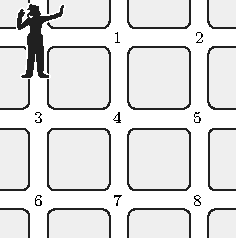
\includegraphics[width=\linewidth]{Images/Capitulo8/Police.pdf}}Una oficial de tráfico está asignada a controlar el tráfico en las ocho intersecciones indicadas en la figura \ref{fig:police}. Se le instruye permanecer en cada intersección durante una hora y luego, ya sea permanecer en la misma intersección o moverse a una intersección vecina. Para evitar establecer un patrón, se le indica elegir su nueva intersección de manera aleatoria, con cada elección posible igualmente probable. Por ejemplo, si se encuentra en la intersección $5$, su próxima intersección puede ser $2$, $4$, $5$, o $8$, cada una con una probabilidad de $1/4$. Cada día, comienza en el lugar donde se detuvo el día anterior. La matriz de transición para esta cadena de Markov es:\\
    \begin{nscenter}
        \begin{tikzpicture}
            \node (A) at (0,0) {$\begin{bmatrix} 1/3 & 1/3 & 0 & 1/5 & 0 & 0 & 0 & 0 \\ 1/3 & 1/3 & 0 & 0 & 1/4 & 0 & 0 & 0 \\ 0 & 0 & 1/3 & 1/5 & 0 & 1/3 & 0 & 0 \\ 1/3 & 0 & 1/3 & 1/5 & 1/4 & 0 & 1/4 & 0 \\ 0 & 1/3 & 0 & 1/5 & 1/4 & 0 & 0 & 1/3 \\ 0 & 0 & 1/3 & 0 & 0 & 1/3 & 1/4 & 0 \\ 0 & 0 & 0 & 1/5 & 0 & 1/3 & 1/4 & 1/3 \\ 0 & 0 & 0 & 0 & 1/4 & 0 & 1/4 & 1/3 \end{bmatrix}$};
            \foreach \i in {1,2,3,...,8}
            {
            \node[black!90!white, xshift=-3.95cm+\i*0.88cm, yshift=0.1cm] at (A.north) {$\i$};
            \node[black!90!white, yshift=1.9cm-\i*0.416cm] at (A.east) {$\i$};
            }
            \node[yshift=0.75cm] at (A.north) {Antigua intersección};
            \node[right,xshift=0.5cm] at (A.east) {Nueva intersección};
        \end{tikzpicture}
    \end{nscenter}
    Si la oficial de tráfico comienza en la intersección $5$, sus ubicaciones probables, hora por hora, están dadas por los vectores de estado que se muestran en la tabla \ref{table:markov2}. Para todos los valores de $n$ mayores que $22$, todos los vectores de estado son iguales a $\mathbb{x}^{(22)}$ con tres decimales. Así, al igual que en los dos primeros ejemplos, los vectores de estado se acercan a un vector fijo a medida que $n$ aumenta.\newpage
    \begin{table*}[h!]
        \centering
        \begin{NiceTabular}{cccccccccccccc}[vlines,cell-space-limits=4pt]
            \CodeBefore
            \rowcolor{black!20!white}{1}
            \columncolor{black!20!white}{1}
            \rowcolor{black!20!white}{2}
            \Body
            \hline
            \Block{2-1}{\diagbox{\raisebox{4pt}{\hspace*{0.1cm} $\mathbb{x}^{(n)}$}}{\raisebox{-0.4cm}{$n$\hspace{0.3cm}}}} & \Block{2-1}{$0$} & \Block{2-1}{$1$} & \Block{2-1}{$2$} & \Block{2-1}{$3$} & \Block{2-1}{$4$} & \Block{2-1}{$5$} & \Block{2-1}{$\cdots$} & \Block{2-1}{$10$} & \Block{2-1}{$\cdots$} & \Block{2-1}{$15$} & \Block{2-1}{$\cdots$} & \Block{2-1}{$21$} & \Block{2-1}{$22$} \\
            \hspace{1.5cm} & \\
            \hline
            $x_1^{(n)}$ & $0$ & $0.000$ & $0.133$ & $0.116$ & $0.130$ & $0.123$ & $\cdots$ & $0.113$ & $\cdots$ & $0.109$ & $\cdots$ & $0.108$ & $0.107$ \\
            $x_2^{(n)}$ & $0$ & $0.250$ & $0.146$ & $0.163$ & $0.140$ & $0.138$ & $\cdots$ & $0.115$ & $\cdots$ & $0.109$ & $\cdots$ & $0.108$ & $0.107$ \\
            $x_3^{(n)}$ & $0$ & $0.000$ & $0.050$ & $0.039$ & $0.067$ & $0.073$ & $\cdots$ & $0.100$ & $\cdots$ & $0.106$ & $\cdots$ & $0.107$ & $0.107$ \\
            $x_4^{(n)}$ & $0$ & $0.250$ & $0.113$ & $0.187$ & $0.162$ & $0.178$ & $\cdots$ & $0.178$ & $\cdots$ & $0.179$ & $\cdots$ & $0.179$ & $0.179$ \\
            $x_5^{(n)}$ & $1$ & $0.250$ & $0.279$ & $0.190$ & $0.190$ & $0.168$ & $\cdots$ & $0.149$ & $\cdots$ & $0.144$ & $\cdots$ & $0.143$ & $0.143$ \\
            $x_6^{(n)}$ & $0$ & $0.000$ & $0.000$ & $0.050$ & $0.056$ & $0.074$ & $\cdots$ & $0.099$ & $\cdots$ & $0.105$ & $\cdots$ & $0.107$ & $0.107$ \\
            $x_7^{(n)}$ & $0$ & $0.000$ & $0.133$ & $0.104$ & $0.131$ & $0.125$ & $\cdots$ & $0.138$ & $\cdots$ & $0.142$ & $\cdots$ & $0.143$ & $0.143$ \\
            $x_8^{(n)}$ & $0$ & $0.250$ & $0.146$ & $0.152$ & $0.124$ & $0.121$ & $\cdots$ & $0.108$ & $\cdots$ & $0.107$ & $\cdots$ & $0.107$ & $0.107$ \\
            \hline
        \end{NiceTabular}
        \caption{~}
        \label{table:markov2}
    \end{table*}\vspace{-0.5cm}
\end{example}

En nuestros ejemplos vimos que los vectores de estado se aproximaban a un vector fijo a medida que aumentaba el número de observaciones. Ahora nos preguntamos si los vectores de estado siempre se aproximan a un vector fijo en una cadena de Markov. Un ejemplo sencillo muestra que este no es siempre el caso.

\begin{example}
    Sean
    $$P = \begin{bmatrix}
        0 & 1 \\
        1 & 0
    \end{bmatrix} \quad \text{ y } \quad \mathbb{x}^{(0)} = \begin{bmatrix}
        1 \\
        0
    \end{bmatrix}$$
    Entonces, dado que $P^2 = I_2$ y $P^3 = P$, tenemos que
    $$\mathbb{x}^{(0)} = \mathbb{x}^{(2)} = \mathbb{x}^{(4)} = \cdots = \begin{bmatrix} 1 \\ 0 \end{bmatrix}$$
    y
    $$\mathbb{x}^{(1)} = \mathbb{x}^{(3)} = \mathbb{x}^{(5)} = \cdots = \begin{bmatrix} 0 \\ 1 \end{bmatrix}$$
    Este sistema oscila indefinidamente entre los dos vectores $\begin{bmatrix} 0 \\ 1 \end{bmatrix}$ y $\begin{bmatrix} 1 \\ 0 \end{bmatrix}$, por lo que no se aproxima a ningún vector fijo.
\end{example}

No obstante, si imponemos una condición simple a la matriz de transición, podemos demostrar que se alcanza un vector de estado fijo. Esta condición se define a continuación.

\begin{definition}
    Una matriz de transición se considera \emph{regular} si, al elevarla a alguna potencia entera, todas sus entradas son positivas.
\end{definition}

Por lo tanto, para una matriz de transición regular $P$, existe un entero positivo $m$ tal que todas las entradas de $P^m$ son positivas. Este es el caso de las matrices de transición en los ejemplos \ref{exam:markov1} y \ref{exam:markov2} con $m = 1$. En el ejemplo \ref{exam:markov5}, resulta que $P^4$ tiene todas las entradas positivas. Por lo tanto, en los tres ejemplos, las matrices de transición son regulares.

Una cadena de Markov con una matriz de transición regular se llama \emph{cadena de Markov regular}. Veremos que toda cadena de Markov regular tiene un vector de estado fijo $\mathbb{q}$ tal que $P^n \mathbb{x}^{(0)}$ se aproxima a $\mathbb{q}$ a medida que $n$ aumenta, para cualquier elección de $\mathbb{x}^{(0)}$. Este resultado es de gran importancia en la teoría de cadenas de Markov y se basa en el siguiente teorema.

\newpage
\infoBulle{No demostraremos este teorema aquí. Para una demostración detallada, consulte un texto más especializado, como J. Kemeny y J. Snell, \emph{Finite Markov Chains} (New York: Springer-Verlag, 1976).}

\begin{theorem}\label{theo:tomarkov2}
    Si $P$ es una matriz de transición regular, entonces a medida que $n \to \infty$,
    $$P^n \to \begin{bmatrix}
        q_1 & q_1 & \cdots & q_1 \\
        q_2 & q_2 & \cdots & q_2 \\
        \vdots & & \ddots & \vdots \\
        q_k & q_k & \cdots & q_k
    \end{bmatrix}$$
    donde los $q_i$ son números positivos tales que $q_1 + q_2 + \cdots + q_k = 1$.
\end{theorem}

Consideremos
$$Q = \begin{bmatrix}
    q_1 & q_1 & \cdots & q_1 \\
    q_2 & q_2 & \cdots & q_2 \\
    \vdots & & \ddots & \vdots \\
    q_k & q_k & \cdots & q_k
\end{bmatrix} \quad \text{ y } \quad \mathbb{q} = \begin{bmatrix}
    q_1 \\
    q_2 \\
    \vdots \\
    q_k
\end{bmatrix}$$
Es decir, $Q$ es una matriz de transición cuyas columnas son todas iguales al vector de probabilidad $\mathbb{q}$. $Q$ tiene la propiedad de que si $\mathbb{x}$ es cualquier vector de probabilidad, entonces
\begin{align*}
    Q\mathbb{x} & = \begin{bmatrix}
        q_1 & q_1 & \cdots & q_1 \\
        q_2 & q_2 & \cdots & q_2 \\
        \vdots & & \ddots & \vdots \\
        q_k & q_k & \cdots & q_k
    \end{bmatrix} \begin{bmatrix}
        x_1 \\
        x_2 \\
        \vdots \\
        x_k
    \end{bmatrix} \\
    & = \begin{bmatrix}
        q_1x_1 + q_1x_2 + \cdots + q_1x_k \\
        q_2x_1 + q_2x_2 + \cdots + q_2x_k \\
        \vdots \\
        q_kx_1 + q_kx_2 + \cdots + q_kx_k
    \end{bmatrix} \\
    & = (x_1 + x_2 + \cdots + x_k) \begin{bmatrix}
        q_1 \\
        q_2 \\
        \vdots \\
        q_k
    \end{bmatrix} \\
    & = (1) \mathbb{q} \\
    & = \mathbb{q}
\end{align*}
Es decir, $Q$ transforma cualquier vector de probabilidad $\mathbb{x}$ en el vector de probabilidad fijo $\mathbb{q}$. Este resultado nos lleva al siguiente teorema.

\begin{theorem}\label{theo:tomarkov3}
    Si $P$ es una matriz de transición regular y $\mathbb{x}$ es cualquier vector de probabilidad, entonces, conforme $n \to \infty$, 
    $$P^n \mathbb{x} \to \begin{bmatrix}
        q_1 \\
        q_2 \\
        \vdots \\
        q_k
    \end{bmatrix} = \mathbb{q}$$
    donde $\mathbb{q}$ es un vector de probabilidad fijo, independiente de $n$, y cuyos componentes son todos positivos.
\end{theorem}

Este resultado se cumple ya que el teorema \ref{theo:tomarkov2} implica que $P^n \to Q$ a medida que $n \to \infty$. Esto, a su vez, implica que $P^n\mathbb{x} \to Q\mathbb{x} = \mathbb{q}$ a medida que $n \to \infty$. Así, para una cadena de Markov regular, el sistema eventualmente se aproxima a un vector de estado fijo $\mathbb{q}$. Este vector $\mathbb{q}$ se llama el \emph{vector de estado estacionario} de la cadena de Markov regular.

Para sistemas con muchos estados, usualmente la técnica más eficiente para calcular el vector de estado estacionario $\mathbb{q}$ es simplemente calcular $P^n \mathbb{x}$ para algún $n$ grande. Nuestros ejemplos ilustran este procedimiento. Cada uno es un proceso de Markov regular, por lo que la convergencia a un vector de estado estacionario está asegurada. Otra forma de calcular el vector de estado estacionario es utilizando el siguiente teorema.

\begin{theorem}\label{theo:tomarkov4}
    El vector de estado estacionario $\mathbb{q}$ de una matriz de transición regular $P$ es el único vector de probabilidad que satisface la ecuación $P \mathbb{q} = \mathbb{q}$.
\end{theorem}

Para entender esto, consideremos la identidad matricial $PP^n = P^{n+1}$. Según el teorema \ref{theo:tomarkov2}, tanto $P^n$ como $P^{n+1}$ se aproximan a $Q$ a medida que $n \to \infty$. Así, tenemos $PQ = Q$. Cualquier columna de esta ecuación matricial da como resultado $P\mathbb{q} = \mathbb{q}$. Para demostrar que $\mathbb{q}$ es el único vector de probabilidad que satisface esta ecuación, supongamos que $\mathbb{r}$ es otro vector de probabilidad tal que $P\mathbb{r} = \mathbb{r}$. Entonces también $P^n\mathbb{r} = \mathbb{r}$ para $n = 1, 2, \dots$. Cuando dejamos que $n \to \infty$, el teorema \ref{theo:tomarkov3} nos lleva a que $\mathbb{q} = \mathbb{r}$.

La ecuación del teorema \ref{theo:tomarkov4} también se puede expresar como un sistema lineal homogéneo
$$(I_k - P)\mathbb{q} = \mathbb{0}$$
donde tiene una solución única, el vector $\mathbb{q}$, con entradas no negativas que satisfacen la condición $q_1 + q_2 + \cdots + q_k = 1$. Podemos aplicar esta técnica para calcular los vectores de estado estacionario en nuestros ejemplos.

\begin{example}
    En el ejemplo \ref{exam:markov2}, la matriz de transición era
    $$P = \begin{bmatrix} 
        0.8 & 0.3 \\ 
        0.2 & 0.7 
    \end{bmatrix}$$
    Entonces, el sistema lineal $(I_2 - P)\mathbb{q} = \mathbb{0}$ es
    $$\begin{bmatrix*}[r]
        0.2 & -0.3 \\
        -0.2 & 0.3
    \end{bmatrix*}\begin{bmatrix}
        q_1 \\
        q_2
    \end{bmatrix} = \begin{bmatrix}
        0 \\
        0
    \end{bmatrix}$$
    Esto lleva a la única ecuación independiente
    $$0.2q_1 - 0.3q_2 = 0$$
    o bien,
    $$q_1 = 1.5q_2$$
    Es decir, la solución general al sistema está dada por
    $$\mathbb{q} = \begin{bmatrix}
        1.5q_2 \\
        q_2
    \end{bmatrix} = q_2 \begin{bmatrix}
        1.5 \\
        1
    \end{bmatrix}$$
    Para que el vector $\mathbb{q}$ sea un vector de probabilidad, la suma de las entradas de $\mathbb{q}$ debe ser igual a $1$. Así,
    $$q_2 = \frac{1}{1.5 + 1} = 0.4$$
    Por consiguiente,
    $$\mathbb{q} = \begin{bmatrix}
        0.6 \\
        0.4
    \end{bmatrix}$$
    es el vector de estado estacionario de esta cadena de Markov regular. Esto significa que a largo plazo, el $60\%$ de los exalumnos harán una donación en un año determinado, y el $40\%$ no lo harán. Observe que esto concuerda con el resultado obtenido numéricamente en el ejemplo \ref{exam:markov3}.
\end{example}

\newpage

\begin{example}
    En el ejemplo \ref{exam:markov1}, la matriz de transición era
    $$P = \begin{bmatrix}
        0.8 & 0.3 & 0.2 \\
        0.1 & 0.2 & 0.6 \\
        0.1 & 0.5 & 0.2
    \end{bmatrix}$$
    Así que el sistema lineal $(I_3 - P)\mathbb{q} = \mathbb{0}$ está dado por
    $$\begin{bmatrix*}[r]
        0.2 & -0.3 & -0.2 \\
        -0.1 & 0.8 & -0.6 \\
        -0.1 & -0.5 & 0.8
    \end{bmatrix*}\begin{bmatrix}
        q_1 \\
        q_2 \\
        q_3
    \end{bmatrix} = \begin{bmatrix}
        0 \\
        0 \\
        0
    \end{bmatrix}$$
    Utilizando el método de reducción de Gauss-Jordan, obtenemos que
    $$\begin{bmatrix}
        1 & 0 & -\dfrac{34}{13} \\[3mm]
        0 & 1 & -\dfrac{14}{13} \\[3mm]
        0 & 0 & \phantom{-}0
    \end{bmatrix}\begin{bmatrix}
        q_1 \\
        q_2 \\
        q_3
    \end{bmatrix} = \begin{bmatrix}
        0 \\
        0 \\
        0
    \end{bmatrix}$$
    Por lo que el sistema lineal original es equivalente al sistema
    \begin{align*}
        q_1 & = \frac{34}{13} q_3 \\
        q_2 & = \frac{14}{13} q_3
    \end{align*}
    Es decir, la solución general al sistema está dada por
    $$\mathbb{q} = \begin{bmatrix}
        \dfrac{34}{13} q_3 \\[3mm]
        \dfrac{14}{13} q_3 \\[3mm]
        q_3
    \end{bmatrix} = q_3 \begin{bmatrix}
        \dfrac{34}{13} \\[3mm] 
        \dfrac{14}{13} \\[3mm]
        1
    \end{bmatrix}$$
    Para que el vector $\mathbb{q}$ sea un vector de probabilidad, la suma de las entradas de $\mathbb{q}$ debe ser igual a $1$. Así,
    $$q_3 = \frac{1}{\dfrac{34}{13} + \dfrac{14}{13} + 1} = \frac{13}{61}$$
    Por consiguiente, el vector de estado estacionario del sistema es
    $$\mathbb{q} = \begin{bmatrix}
        \dfrac{34}{61} \\[2mm]
        \dfrac{14}{61} \\[2mm]
        \dfrac{13}{61}
    \end{bmatrix} = \begin{bmatrix}
        0.5573 \dots \\
        0.2295 \dots \\
        0.2131 \dots
    \end{bmatrix}$$
    Esto concuerda con el resultado obtenido numéricamente en la tabla \ref{table:markov1}. Los valores de $\mathbb{q}$ dan las probabilidades a largo plazo de que cualquier coche sea devuelto a la ubicación $1$, $2$ o $3$, respectivamente. Si la agencia de alquiler de coches tiene una flota de $1 \, 000$ coches, debería diseñar sus instalaciones de manera que haya al menos $558$ espacios en la ubicación $1$, al menos $230$ espacios en la ubicación $2$, y al menos $214$ espacios en la ubicación $3$.
\end{example}

\begin{example}
    Tomemos la matriz de transición del ejemplo \ref{exam:markov5}. No daremos los detalles de los cálculos, pero simplemente afirmaremos que la única solución del vector de probabilidad para el sistema lineal $(I_8 - P)\mathbb{q} = \mathbb{0}$ es\newpage
    $$\mathbb{q} = \frac{1}{28} \begin{bmatrix}
        3 \\
        3 \\
        3 \\
        5 \\
        4 \\
        3 \\
        4 \\
        3
    \end{bmatrix} = \begin{bmatrix}
        0.1071\dots \\
        0.1071\dots \\
        0.1071\dots \\
        0.1785\dots \\
        0.1428\dots \\
        0.1071\dots \\
        0.1428\dots \\
        0.1071\dots \\
    \end{bmatrix}$$
    Esto concuerda con el resultado obtenido numéricamente en la tabla \ref{table:markov2}. Los valores de este vector muestran la proporción de tiempo que la oficial de tráfico pasa en cada intersección a largo plazo. Por lo tanto, si se busca que pase la misma cantidad de tiempo en todas las intersecciones, la estrategia de moverse aleatoriamente con probabilidades iguales entre intersecciones no es adecuada.
\end{example}

\section{Teoría de grafos}

Existen innumerables ejemplos de conjuntos finitos donde sus elementos están relacionados de alguna manera. Por ejemplo, el conjunto podría estar compuesto por personas, animales, países, empresas, equipos deportivos o ciudades. La relación entre dos elementos, $A$ y $B$, podría ser que la persona $A$ domina a la persona $B$, el animal $A$ se alimenta del animal $B$, el país $A$ apoya militarmente al país $B$, la empresa $A$ vende su producto a la empresa $B$, el equipo deportivo $A$ siempre vence al equipo deportivo $B$, o la ciudad $A$ tiene un vuelo directo a la ciudad $B$.

Ahora mostraremos cómo la teoría de \emph{grafos dirigidos} puede utilizarse para modelar matemáticamente relaciones como estas.

\subsection*{Grafos dirigidos}
\sideFigure[\label{fig:examgrafos1}]{
\begin{tikzpicture}
    %%%%% COORDENADAS %%%%%
    \coordinate (P1) {};
    \coordinate[above right=1cm and 2.5cm of P1] (P2) {};
    \coordinate[below right=1.1cm and 0.5cm of P2] (P3) {};
    \coordinate[below left=1.25cm and 0.1cm of P3] (P4) {};
    \coordinate[above left=0.25cm and 1.75cm of P4] (P5) {};
    \coordinate[above right=0.5cm and 3cm of P5] (P6) {};
    \coordinate[above left=1.25cm and 0.1cm of P6] (P7) {};
    %%%%% PUNTOS %%%%%
    \filldraw (P1) circle (1.75pt) node[below] {$P_1$};
    \filldraw (P2) circle (1.75pt) node[above] {$P_2$};
    \filldraw (P3) circle (1.75pt) node[right,yshift=-0.1cm] {$P_3$};
    \filldraw (P4) circle (1.75pt) node[below] {$P_4$};
    \filldraw (P5) circle (1.75pt) node[right] {$P_5$};
    \filldraw (P6) circle (1.75pt) node[above] {$P_6$};
    \filldraw (P7) circle (1.75pt) node[above] {$P_7$};
    %%%%% FLECHAS %%%%%
    \draw[postaction={decorate,decoration={markings,mark=at position 0.5 with {\arrow{Stealth[scale=1.25]}}}}] (P1) .. controls ($(P1)!.4!(P2) + (0,0.25)$) and ($(P1)!.6!(P2) + (0,0.25)$) .. (P2);
    \draw[postaction={decorate,decoration={markings,mark=at position 0.5 with {\arrow{Stealth[scale=1.25]}}}}] (P1) .. controls ($(P1)!.4!(P3) + (0,-0.5)$) and ($(P1)!.6!(P3) + (0,-0.5)$) .. (P3);
    \draw[postaction={decorate,decoration={markings,mark=at position 0.6 with {\arrow{Stealth[scale=1.25]}}}}] (P3) .. controls ($(P3)!.4!(P7) + (0,-0.2)$) and ($(P3)!.6!(P7) + (0,0.2)$) .. (P7);
    \draw[postaction={decorate,decoration={markings,mark=at position 0.5 with {\arrow{Stealth[scale=1.25]}}}}] (P4) .. controls ($(P4)!.4!(P6) + (0,-0.25)$) and ($(P4)!.6!(P6) + (0,-0.25)$) .. (P6);
    \draw[postaction={decorate,decoration={markings,mark=at position 0.4 with {\arrow[>={Stealth[scale=1.25]}]{<}}}}] (P2) .. controls ($(P2)!.4!(P3) + (0.25,0)$) and ($(P2)!.6!(P3) + (0.25,0)$) .. (P3);
    \draw[postaction={decorate,decoration={markings,mark=at position 0.8 with {\arrow[>={Stealth[scale=1.25]}]{>}}}}] (P2) .. controls ($(P2)!.4!(P3) + (0.25,0)$) and ($(P2)!.6!(P3) + (0.25,0)$) .. (P3);
\end{tikzpicture}
}

Un grafo dirigido es un conjunto finito de elementos $\{P_1, P_2, \dots, P_n\}$ junto con una colección finita de pares ordenados $(P_i, P_j)$ de elementos distintos de este conjunto, sin repetir ningún par ordenado. Los elementos del conjunto se llaman vértices, y los pares ordenados se llaman aristas dirigidas del grafo dirigido. Usamos la notación $P_i \rightarrow P_j$ (que se lee “$P_i$ está conectado a $P_j$”) para indicar que la arista dirigida $(P_i, P_j)$ pertenece al grafo dirigido. Geométricamente, podemos visualizar un grafo dirigido (figura \ref{fig:examgrafos1}) representando los vértices como puntos en el plano y representando la arista dirigida $P_i \rightarrow P_j$ dibujando una línea o arco desde el vértice $P_i$ hasta el vértice $P_j$, con una flecha que apunta de $P_i$ a $P_j$. Si tanto $P_i \rightarrow P_j$ como $P_j \rightarrow P_i$ son ciertos (denotado $P_i \leftrightarrow P_j$), dibujamos una sola línea entre $P_i$ y $P_j$ con dos flechas apuntando en direcciones opuestas (como con $P_2$ y $P_3$ en la figura).

Como se muestra en la figura \ref{fig:examgrafos1}, un grafo dirigido puede tener componentes separadas de vértices que están conectados solo entre sí; y algunos vértices, como $P_5$, pueden no estar conectados con ningún otro vértice. Además, dado que $P_i \rightarrow P_i$ no está permitido en un grafo dirigido, un vértice no puede estar conectado consigo mismo por un solo arco que no pase por ningún otro vértice.

La figura \ref{fig:examgrafos2} muestra diagramas que representan tres ejemplos más de grafos dirigidos.\newpage
\begin{figure*}[h!]
    \centering
    \subfloat[\label{fig:examgrafos2a}]{
    \begin{tikzpicture}
        %%%%% COORDENADAS %%%%%
        \coordinate (P1) {};
        \coordinate[above=3cm of P1] (P2) {};
        \coordinate[right=3.5cm of P2] (P3) {};
        \coordinate[below=3cm of P3] (P4) {};
        \draw (P1) -- (P2) -- (P3) -- (P4);
        %%%%% PUNTOS %%%%%
        \filldraw (P1) circle (1.75pt) node[left] {$P_1$};
        \filldraw (P2) circle (1.75pt) node[left] {$P_2$};
        \filldraw (P3) circle (1.75pt) node[right] {$P_3$};
        \filldraw (P4) circle (1.75pt) node[right] {$P_4$};
        %%%%% FLECHAS %%%%%
        \draw[-{Stealth[scale=1.25]}] (P1) -- ($(P1)!.5!(P2)$);
        \draw[{Stealth[scale=1.25]}-{Stealth[scale=1.25]}] ($(P2)!.25!(P3)$) -- ($(P2)!.75!(P3)$);
        \draw[-{Stealth[scale=1.25]}] (P3) -- ($(P3)!.5!(P4)$);
    \end{tikzpicture}
    } \hfill
    \subfloat[\label{fig:examgrafos2b}]{
    \begin{tikzpicture}
        %%%%% COORDENADAS %%%%%
        \coordinate (P1) {};
        \coordinate[above right=1.25cm and 0.15cm of P1] (P2) {};
        \coordinate[above right=1.75cm and 2.25cm of P2] (P3) {};
        \coordinate[below right=1.15cm and 2cm of P3] (P4) {};
        \coordinate[below right=0.15cm and 2cm of P1] (P5) {};
        \draw (P1) -- (P2) -- (P3) -- (P4) -- (P5) -- (P1) -- cycle;
        \draw (P5) -- (P2);
        \draw[name path=P2--P4] (P2) -- (P4);
        \draw[name path=P5--P3] (P5) -- (P3);
        \path[name intersections={of=P2--P4 and P5--P3,by=P}];
        %%%%% PUNTOS %%%%%
        \filldraw (P1) circle (1.75pt) node[left] {$P_1$};
        \filldraw (P2) circle (1.75pt) node[left] {$P_2$};
        \filldraw (P3) circle (1.75pt) node[above] {$P_3$};
        \filldraw (P4) circle (1.75pt) node[right] {$P_4$};
        \filldraw (P5) circle (1.75pt) node[below] {$P_5$};
        %%%%% FLECHAS %%%%%
        \draw[-{Stealth[scale=1.25]}] (P1) -- ($(P1)!.5!(P2)$);
        \draw[-{Stealth[scale=1.25]}] (P2) -- ($(P2)!.5!(P3)$);
        \draw[-{Stealth[scale=1.25]}] (P3) -- ($(P3)!.5!(P4)$);
        \draw[-{Stealth[scale=1.25]}] (P4) -- ($(P4)!.5!(P5)$);
        \draw[-{Stealth[scale=1.25]}] (P1) -- ($(P1)!.5!(P5)$);
        \draw[-{Stealth[scale=1.25]}] (P5) -- ($(P5)!.5!(P2)$);
        \draw[{Stealth[scale=1.25]}-{Stealth[scale=1.25]}] ($(P2)!.25!(P4)$) -- ($(P2)!.75!(P4)$);
        \draw[-{Stealth[scale=1.25]}] (P) -- ($(P)!.5!(P3)$);
    \end{tikzpicture}
    } \hfill
    \subfloat[\label{fig:examgrafos2c}]{
    \begin{tikzpicture}
        \def\radius{1.75}
        %%%%% COORDENADAS %%%%%%
        \coordinate (O) {};
        \coordinate (P1) at ($(O) +(0.75*180:\radius)$) {};
        \coordinate (P2) at ($(O) +(1.25*180:\radius)$) {};
        \coordinate (P3) at ($(O) +(1.6*180:\radius)$) {};
        \coordinate (P4) at ($(O) +(0*180:\radius)$) {};
        \draw (O) circle[radius=\radius];
        %%%%% PUNTOS %%%%%
        \filldraw (P1) circle (1.75pt) node[above left] {$P_1$};
        \filldraw (P2) circle (1.75pt) node[left,yshift=-0.1cm] {$P_2$};
        \filldraw (P3) circle (1.75pt) node[below] {$P_3$};
        \filldraw (P4) circle (1.75pt) node[right] {$P_4$};
        %%%%% FLECHAS %%%%%
        \draw[
            decoration={
                markings, mark=at position 0.187 with {\arrow[>={Stealth[scale=1.25]}]{>}}
            },
            postaction={decorate}
        ] (O) circle (\radius);
        \draw[
            decoration={
                markings, mark=at position 0.45 with {\arrow[>={Stealth[scale=1.25]}]{<}}
            },
            postaction={decorate}
        ] (O) circle (\radius);
        \draw[
            decoration={
                markings, mark=at position 0.55 with {\arrow[>={Stealth[scale=1.25]}]{>}}
            },
            postaction={decorate}
        ] (O) circle (\radius);
        \draw[
            decoration={
                markings, mark=at position 0.725 with {\arrow[>={Stealth[scale=1.25]}]{>}}
            },
            postaction={decorate}
        ] (O) circle (\radius);
        \draw[
            decoration={
                markings, mark=at position 0.92 with {\arrow[>={Stealth[scale=1.25]}]{>}}
            },
            postaction={decorate}
        ] (O) circle (\radius);
        \draw[postaction={decorate,decoration={markings,mark=at position 0.5 with {\arrow{Stealth[scale=1.25]}}}}] (P3) .. controls ($(O) + (0.5,0)$) and ($(O) + (0,0.5)$) .. (P1);
    \end{tikzpicture}
    }
    \caption{~}
    \label{fig:examgrafos2}
\end{figure*}

\noindent Con un grafo dirigido de $n$ vértices, podemos asociar una matriz de tamaño $n \times n$ denotada como $M = \llparenthesis m_{ij} \rrparenthesis$, llamada \emph{matriz de vértices} del grafo dirigido. Sus elementos se definen por
$$m_{ij} = \begin{cases}
    1, & \text{ si } P_i \rightarrow P_j \\
    0, & \text{ en cualquier otro caso}
\end{cases}$$
para $i$, $j = 1, 2, \dots, n$. Para los tres grafos dirigidos en la figura \ref{fig:examgrafos2}, las matrices de vértices correspondientes son:
\begin{align*}
    \text{Figura \ref{fig:examgrafos2a}}: & & M & = \begin{bmatrix} 0 & 1 & 0 & 0 \\ 0 & 0 & 1 & 0 \\ 0 & 1 & 0 & 1 \\ 0 & 0 & 0 & 0 \end{bmatrix} \\
    \text{Figura \ref{fig:examgrafos2b}}: & & M & = \begin{bmatrix} 0 & 1 & 0 & 0 & 1 \\ 0 & 0 & 1 & 1 & 0 \\ 0 & 0 & 0 & 1 & 0 \\ 0 & 1 & 0 & 0 & 1 \\ 0 & 1 & 1 & 0 & 0 \end{bmatrix} \\
    \text{Figura \ref{fig:examgrafos2c}}: & & M & = \begin{bmatrix} 0 & 1 & 0 & 0 \\ 1 & 0 & 1 & 0 \\ 1 & 0 & 0 & 1 \\ 1 & 0 & 0 & 0 \end{bmatrix}
\end{align*}
Por definición, las matrices de vértices tienen las siguientes dos propiedades:
\begin{enumerate}[label=\roman*)]
    \item Todos los elementos son $0$ o $1$.
    \item Todos los elementos en la diagonal son $0$.
\end{enumerate}
\sideFigure[\label{fig:matvergraf}]{
\begin{tikzpicture}
    %%%%% COORDENADAS %%%%%
    \coordinate (P1) {};
    \coordinate[below right=1cm and 2cm of P1] (P2) {};
    \coordinate[above right=2.5cm and 0.5cm of P2] (P3) {};
    \coordinate[below right=1cm and 2cm of P3] (P4) {};
    %%%%% PUNTOS %%%%%
    \filldraw (P1) circle (1.75pt) node[left] {$P_1$};
    \filldraw (P2) circle (1.75pt) node[below] {$P_2$};
    \filldraw (P3) circle (1.75pt) node[above] {$P_3$};
    \filldraw (P4) circle (1.75pt) node[below] {$P_4$};
    %%%%% FLECHAS %%%%%
    \draw[postaction={decorate,decoration={markings,mark=at position 0.5 with {\arrow{Stealth[scale=1.25]}}}}] (P1) .. controls ($(P1)!.3!(P2) + (0,-0.5)$) and ($(P1)!.7!(P2) + (0,-0.5)$) .. (P2);
    \draw[postaction={decorate,decoration={markings,mark=at position 0.5 with {\arrow{Stealth[scale=1.25]}}}}] (P2) .. controls ($(P2)!.3!(P3) + (0.5,0)$) and ($(P2)!.7!(P3) + (0.5,0)$) .. (P3);
    \draw[postaction={decorate,decoration={markings,mark=at position 0.3 with {\arrow[>={Stealth[scale=1.25]}]{<}}}}] (P1) .. controls ($(P1)!.4!(P3) + (0,0.5)$) and ($(P1)!.6!(P3) + (0,0.5)$) .. (P3);
    \draw[postaction={decorate,decoration={markings,mark=at position 0.7 with {\arrow[>={Stealth[scale=1.25]}]{>}}}}] (P1) .. controls ($(P1)!.4!(P3) + (0,0.5)$) and ($(P1)!.6!(P3) + (0,0.5)$) .. (P3);
    \draw[postaction={decorate,decoration={markings,mark=at position 0.5 with {\arrow{Stealth[scale=1.25]}}}}] (P3) .. controls ($(P3)!.3!(P4) + (0,0.3)$) and ($(P3)!.7!(P4) + (0,0.3)$) .. (P4);
\end{tikzpicture}
}
Inversamente, cualquier matriz con estas dos propiedades determina un grafo dirigido único que tiene dicha matriz como su matriz de vértices. Por ejemplo, la matriz
$$M = \begin{bmatrix}
    0 & 1 & 1 & 0 \\
    0 & 0 & 1 & 0 \\
    1 & 0 & 0 & 1 \\
    0 & 0 & 0 & 0
\end{bmatrix}$$
determina el grafo dirigido en la figura \ref{fig:matvergraf}.

\begin{example}\label{exam:graf1}
    \sideFigure[\label{fig:grapfam}]{\centering
    \begin{tikzpicture}
        %%%%% COORDENADAS %%%%%
        \coordinate (D) {};
        \coordinate[above right=2cm and 2cm of D] (OS) {};
        \coordinate[right=4cm of D] (F) {};
        \coordinate[above=4cm of F] (YS) {};
        \coordinate[left=4cm of YS] (M) {};
        \draw (D) rectangle (YS);
        \draw (M) -- (F);
        \draw (OS) -- (YS);
        %%%%% PUNTOS %%%%%
        \filldraw (D) circle (1.75pt) node[left] {$H$};
        \filldraw (F) circle (1.75pt) node[right] {$P$};
        \filldraw (YS) circle (1.75pt) node[right] {$B$};
        \filldraw (M) circle (1.75pt) node[left] {$M$};
        \filldraw (OS) circle (1.75pt) node[below left] {$A$};
        %%%%% FLECHAS %%%%%
        \draw[-{Stealth[scale=1.25]}] (D) -- ($(D)!.5!(F)$);
        \draw[-{Stealth[scale=1.25]}] (M) -- ($(M)!.5!(D)$);
        \draw[-{Stealth[scale=1.25]}] (M) -- ($(M)!.5!(OS)$);
        \draw[-{Stealth[scale=1.25]}] (F) -- ($(F)!.5!(OS)$);
        \draw[-{Stealth[scale=1.25]}] (OS) -- ($(OS)!.5!(YS)$);
        \draw[-{Stealth[scale=1.25]}] (YS) -- ($(YS)!.5!(M)$);
        \draw[-{Stealth[scale=1.25]}] (F) -- ($(F)!.5!(YS)$);
    \end{tikzpicture}
    }
    Una familia está compuesta por una madre ($M$), un padre ($P$), una hija ($H$) y dos hijos, el mayor ($A$) y el menor ($B$). Los miembros de esta familia tienen diversas formas de influencia o poder entre ellos. La madre ($M$) puede influir en la hija ($H$) y también en el hijo mayor ($A$). El padre ($P$) tiene la capacidad de influir en ambos hijos, es decir, en el mayor ($A$) y en el menor ($B$). Por otro lado, la hija ($H$) puede influir en el padre ($P$), estableciendo así\newpage
    \sideFigure[\label{fig:ajedreztab}]{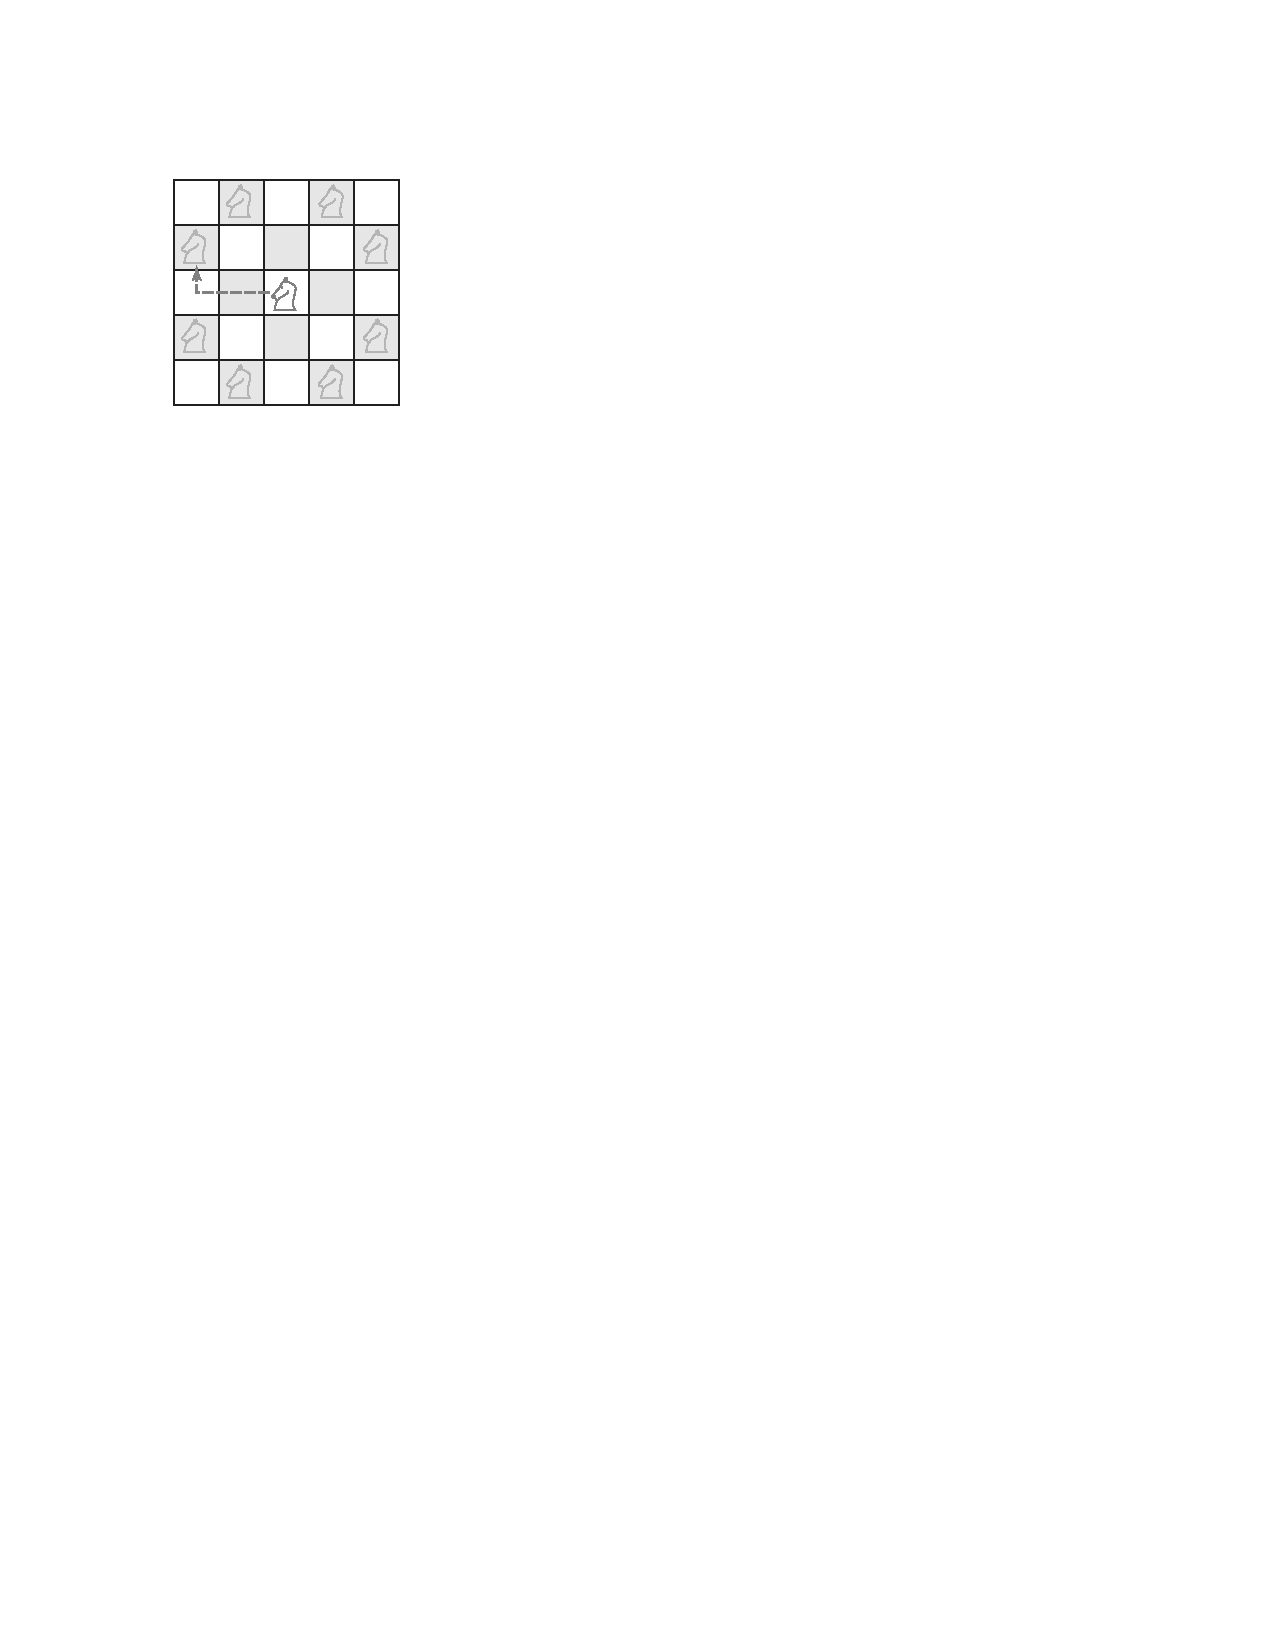
\includegraphics[width=\linewidth]{Images/Capitulo8/Chess.pdf}}
    \sideFigure[\label{fig:ajedreztab2}]{\centering
    \begin{tikzpicture}
        \def\n{3}
        \def\m{3}
        \def\s{1.25cm}
        \draw grid[step=\s] (\n*\s, \m*\s);
        \foreach[evaluate] \x in {1,...,\n} {
            \foreach[evaluate={
                \zt = int(\x + \n*min(\y-1,\m+\y));
                \zb = int(\x + (\n-2)*min(\y-1,\m+\y)+3);
                }] \y in {1,...,\m} {
                \node[font=\large] at ({\s*(0.5+(\x-1))},{\s*(\m+0.5-\y)}) {$\ifthenelse{\y>3}{\ifthenelse{\x>3}{\zb}}{\zt}$};
                }
            };
    \end{tikzpicture}
    }
    \sideFigure[\label{fig:ajedreztab3}]{\centering
    \begin{tikzpicture}[font=\small]
        \def\dist{1.75cm}
        %%%%% COORDENADAS %%%%%
        \coordinate (P1) {};
        \coordinate[right=\dist of P1] (P2) {};
        \coordinate[right=\dist of P2] (P3) {};
        \coordinate[below=\dist of P3] (P6) {};
        \coordinate[left=\dist of P6] (P5) {};
        \coordinate[left=\dist of P5] (P4) {};
        \coordinate[below=\dist of P4] (P7) {};
        \coordinate[right=\dist of P7] (P8) {};
        \coordinate[right=\dist of P8] (P9) {};
        %%%%% FLECHAS %%%%%
        \draw (P1) -- (P8) -- (P3) -- (P4) -- (P9) -- (P2) -- (P7) -- (P6) -- (P1);
        \draw[{Stealth[scale=1.25]}-{Stealth[scale=1.25]}] ($(P1)!.1!(P8)$) -- ($(P1)!.9!(P8)$);
        \draw[{Stealth[scale=1.25]}-{Stealth[scale=1.25]}] ($(P8)!.1!(P3)$) -- ($(P8)!.9!(P3)$);
        \draw[{Stealth[scale=1.25]}-{Stealth[scale=1.25]}] ($(P3)!.1!(P4)$) -- ($(P3)!.9!(P4)$);
        \draw[{Stealth[scale=1.25]}-{Stealth[scale=1.25]}] ($(P4)!.1!(P9)$) -- ($(P4)!.9!(P9)$);
        \draw[{Stealth[scale=1.25]}-{Stealth[scale=1.25]}] ($(P9)!.1!(P2)$) -- ($(P9)!.9!(P2)$);
        \draw[{Stealth[scale=1.25]}-{Stealth[scale=1.25]}] ($(P2)!.1!(P7)$) -- ($(P2)!.9!(P7)$);
        \draw[{Stealth[scale=1.25]}-{Stealth[scale=1.25]}] ($(P7)!.1!(P6)$) -- ($(P7)!.9!(P6)$);
        \draw[{Stealth[scale=1.25]}-{Stealth[scale=1.25]}] ($(P6)!.1!(P1)$) -- ($(P6)!.9!(P1)$);
        %%%%% PUNTOS %%%%%
        \filldraw (P1) circle (1.75pt) node[above,minimum height=2em] {$1$};
        \filldraw (P2) circle (1.75pt) node[above,minimum height=2em] {$2$};
        \filldraw (P3) circle (1.75pt) node[above,minimum height=2em] {$3$};
        \filldraw (P4) circle (1.75pt) node[left,minimum width=2em] {$4$};
        \filldraw (P5) circle (1.75pt) node[above,minimum height=2em] {$5$};
        \filldraw (P6) circle (1.75pt) node[right,minimum width=2em] {$6$};
        \filldraw (P7) circle (1.75pt) node[below,minimum height=2em] {$7$};
        \filldraw (P8) circle (1.75pt) node[below,minimum height=2em] {$8$};
        \filldraw (P9) circle (1.75pt) node[below,minimum height=2em] {$9$};
    \end{tikzpicture}
    }
    \sideFigure[\label{fig:ajedreztab4}]{\centering
    \begin{tikzpicture}[font=\small, every node/.style={minimum size=2em}]
        \def\radius{2}
        %%%%% COORDENADAS %%%%%%
        \coordinate (O) {};
        \coordinate (P4) at ($(O) +(0*180:\radius)$) {};
        \coordinate (P3) at ($(O) +(0.25*180:\radius)$) {};
        \coordinate (P8) at ($(O) +(0.5*180:\radius)$) {};
        \coordinate (P1) at ($(O) +(0.75*180:\radius)$) {};
        \coordinate (P6) at ($(O) +(1*180:\radius)$) {};
        \coordinate (P7) at ($(O) +(1.25*180:\radius)$) {};
        \coordinate (P2) at ($(O) +(1.5*180:\radius)$) {};
        \coordinate (P9) at ($(O) +(1.75*180:\radius)$) {};
        %%%%% FLECHAS %%%%%
        \foreach \i in {0,1,2,...,7} {
        \draw[
            decoration={
                markings, mark=at position 0.0375+0.125*\i with {\arrow[>={Stealth[scale=1.25]}]{<}}
            },
            postaction={decorate}
        ] (O) circle (\radius);
        \draw[
            decoration={
                markings, mark=at position 0.1+0.125*\i with {\arrow[>={Stealth[scale=1.25]}]{>}}
            },
            postaction={decorate}
        ] (O) circle (\radius);
        }
        %%%%% PUNTOS %%%%%
        \filldraw (O) circle (1.75pt) node[above] {$5$};
        \filldraw (P4) circle (1.75pt) node[right] {$4$};
        \filldraw (P3) circle (1.75pt) node[right,yshift=0.1cm] {$3$};
        \filldraw (P8) circle (1.75pt) node[above] {$8$};
        \filldraw (P1) circle (1.75pt) node[left,yshift=0.1cm] {$1$};
        \filldraw (P6) circle (1.75pt) node[left,yshift=-0.1cm] {$6$};
        \filldraw (P7) circle (1.75pt) node[left,yshift=-0.1cm] {$7$};
        \filldraw (P2) circle (1.75pt) node[below] {$2$};
        \filldraw (P9) circle (1.75pt) node[right,yshift=-0.1cm] {$9$};
    \end{tikzpicture}
    }
    \noindent una dinámica única. Además, el hijo mayor ($A$) tiene la capacidad de influir en el hijo menor ($B$). Finalmente, el hijo menor ($B$) puede ejercer influencia sobre la madre ($M$). Podemos modelar este patrón de influencia familiar con un grafo dirigido cuyos vértices son los cinco miembros de la familia. Si el miembro de la familia $A$ influye en el miembro de la familia $B$, escribimos $A \rightarrow B$. La figura \ref{fig:grapfam} es el grafo dirigido resultante, donde hemos utilizado las anteriores designaciones para los cinco miembros de la familia. La matriz de vértices de este grafo dirigido es\\
    \begin{nscenter}
        \begin{tikzpicture}
            \node (A) at (0,0) {$\begin{bmatrix} 0 & 0 & 1 & 1 & 0 \\ 0 & 0 & 0 & 1 & 1 \\ 0 & 1 & 0 & 0 & 0 \\ 0 & 0 & 0 & 0 & 1 \\ 1 & 0 & 0 & 0 & 0 \end{bmatrix}$};
            \node[black!90!white, xshift=-1cm, yshift=0.1cm] at (A.north) {$M$};
            \node[black!90!white, xshift=-0.5cm, yshift=0.1cm] at (A.north) {$P$};
            \node[black!90!white, yshift=0.1cm] at (A.north) {$H$};
            \node[black!90!white, xshift=0.5cm, yshift=0.1cm] at (A.north) {$A$};
            \node[black!90!white, xshift=1cm, yshift=0.1cm] at (A.north) {$B$};
            \node[black!90!white, yshift=0.85cm, xshift=-0.1cm] at (A.west) {$M$};
            \node[black!90!white, yshift=0.47cm, xshift=-0.1cm] at (A.west) {$P$};
            \node[black!90!white, yshift=0.05cm, xshift=-0.1cm] at (A.west) {$H$};
            \node[black!90!white, yshift=-0.35cm, xshift=-0.1cm] at (A.west) {$A$};
            \node[black!90!white, yshift=-0.8cm, xshift=-0.1cm] at (A.west) {$B$};
        \end{tikzpicture}
    \end{nscenter}
\end{example}

\begin{example}
    En ajedrez, el caballo se mueve en un patrón en forma de “L” sobre el tablero. Para el tablero en la figura \ref{fig:ajedreztab}, puede moverse horizontalmente dos casillas y luego verticalmente una casilla, o puede moverse verticalmente dos casillas y luego horizontalmente una casilla. Así, desde la casilla central en la figura, el caballo puede moverse a cualquiera de las ocho casillas sombreadas marcadas. Supongamos que el caballo está restringido a las nueve casillas numeradas en la figura \ref{fig:ajedreztab2}. Si con $i \to j$ se quiere decir que el caballo puede moverse de la casilla $i$ a la casilla $j$, el grafo dirigido en la figura \ref{fig:ajedreztab3} ilustra todos los movimientos posibles que el caballo puede realizar entre estas nueve casillas. En la figura \ref{fig:ajedreztab4} hemos “desenredado” la figura \ref{fig:ajedreztab3} para hacer más claro el patrón de movimientos posibles. La matriz de vértices de este grafo dirigido es
    $$M = \begin{bmatrix}
        0 & 0 & 0 & 0 & 0 & 1 & 0 & 1 & 0 \\
        0 & 0 & 0 & 0 & 0 & 0 & 1 & 0 & 1 \\
        0 & 0 & 0 & 1 & 0 & 0 & 0 & 1 & 0 \\
        0 & 0 & 1 & 0 & 0 & 0 & 0 & 0 & 1 \\
        0 & 0 & 0 & 0 & 0 & 0 & 0 & 0 & 0 \\
        1 & 0 & 0 & 0 & 0 & 0 & 1 & 0 & 0 \\
        0 & 1 & 0 & 0 & 0 & 1 & 0 & 0 & 0 \\
        1 & 0 & 1 & 0 & 0 & 0 & 0 & 0 & 0 \\
        0 & 1 & 0 & 1 & 0 & 0 & 0 & 0 & 0 
    \end{bmatrix}$$
\end{example}

En el ejemplo \ref{exam:graf1}, el padre no puede influir directamente a la madre; es decir, $P \to M$ no es cierto. Sin embargo, puede influir en el hijo menor, quien a su vez puede influir en la madre. Esto se escribe como $P \to B \to M$ y se denomina una conexión de $2$ pasos de $P$ a $M$. De manera similar, $M \to H$ es una conexión de $1$ paso, mientras que $P \to A \to B \to M$ es una conexión de $3$ pasos, y así sucesivamente.

Consideremos ahora una técnica para determinar el número de todas las posibles conexiones de $r$ pasos ($r = 1, 2, \dots$) desde un vértice $P_i$ hasta otro vértice $P_j$ en un grafo dirigido arbitrario (esto incluye el caso en que $P_i$ y $P_j$ sean el mismo vértice). El número de conexiones de $1$ paso desde $P_i$ hasta $P_j$ es simplemente $m_{ij}$. Es decir, hay cero o una conexión de $1$ paso desde $P_i$ hasta $P_j$, dependiendo de si $m_{ij}$ es cero o uno. Para el número de conexiones de $2$ pasos, consideramos el cuadrado de la matriz de vértices. Si designamos $m_{ij}^{(2)}$ como el elemento $(i, j)$-ésimo de $M^2$, tenemos que
\begin{equation}
    m_{ij}^{(2)} = m_{i1}m_{ij} + m_{i2}m_{2j} + \cdots + m_{in}m_{nj} \label{eq:grafos1}
\end{equation}
Ahora bien, si $m_{i1} = m_{1j} = 1$, hay una conexión de $2$ pasos $P_i \to P_1 \to P_j$ desde $P_i$ hasta $P_j$. Sin embargo, si $m_{i1}$ o $m_{1j}$ es cero, dicha conexión de $2$ pasos no es posible. Por lo tanto, $P_i \to P_1 \to P_j$ es una conexión de $2$ pasos solo si $m_{i1}m_{1j} = 1$. De manera similar, para cualquier $k = 1, 2, \dots, n$, $P_i \to P_k \to P_j$ es una conexión de $2$ pasos desde $P_i$ hasta $P_j$ solo si el término $m_{ik}m_{kj}$ en el lado derecho de \eqref{eq:grafos1} es uno; de lo contrario, el término es cero. Así, el lado derecho de \eqref{eq:grafos1} representa el número total de conexiones de $2$ pasos desde $P_i$ hasta $P_j$.

Un razonamiento similar se puede aplicar para encontrar el número de conexiones de $3$, $4$, $\dots$, $r$ pasos desde $P_i$ hasta $P_j$. En general, obtenemos el siguiente resultado.

\begin{theorem}\label{theo:rconexiones}
    Sea $M$ la matriz de vértices de un grafo dirigido y sea $m^{(r)}_{ij}$ el elemento $(i, j)$-ésimo de $M^r$. Entonces, $m^{(r)}_{ij}$ es igual al número de conexiones de $r$ pasos desde $P_i$ hasta $P_j$.
\end{theorem}

\begin{example}
    \sideFigure[\label{fig:examgrafoss3}]{\centering
    \begin{tikzpicture}
        %%%%% COORDENADAS %%%%%
        \coordinate (P1) {};
        \coordinate[above right=3cm and 3cm of P1] (P2) {};
        \coordinate[below right=3.1cm and 1.4cm of P2] (P3) {};
        \coordinate[below left=2.5cm and 2.9cm of P3] (P4) {};
        %%%%% PUNTOS %%%%%
        \filldraw (P1) circle (1.75pt) node[left] {$P_1$};
        \filldraw (P2) circle (1.75pt) node[above] {$P_2$};
        \filldraw (P3) circle (1.75pt) node[right] {$P_3$};
        \filldraw (P4) circle (1.75pt) node[below] {$P_4$};
        %%%%% FLECHAS %%%%%
        \draw (P1) -- (P2) -- (P3) -- (P4);
        \draw[name path=P1--P3] (P1) -- (P3);
        \draw[name path=P2--P4] (P2) -- (P4);
        \path[name intersections={of=P1--P3 and P2--P4,by=P}];
        \draw[{Stealth[scale=1.25]}-{Stealth[scale=1.25]}] ($(P1)!.25!(P2)$) -- ($(P1)!.75!(P2)$);
        \draw[-{Stealth[scale=1.25]}] (P2) -- ($(P2)!.5!(P3)$);
        \draw[{Stealth[scale=1.25]}-{Stealth[scale=1.25]}] ($(P3)!.25!(P4)$) -- ($(P3)!.75!(P4)$);
        \draw[-{Stealth[scale=1.25]}] (P) -- ($(P)!.5!(P1)$);
        \draw[-{Stealth[scale=1.25]}] (P) -- ($(P)!.5!(P2)$);
        \draw[-{Stealth[scale=1.25]}] (P) -- ($(P)!.5!(P3)$);
    \end{tikzpicture}
    }
    La figura \ref{fig:examgrafoss3} es el mapa de rutas de una pequeña aerolínea que opera en las cuatro ciudades $P_1$, $P_2$, $P_3$, y $P_4$. Como un grafo dirigido, su matriz de vértices es
    $$M = \begin{bmatrix}
        0 & 1 & 1 & 0 \\
        1 & 0 & 1 & 0 \\
        1 & 0 & 0 & 1 \\
        0 & 1 & 1 & 0
    \end{bmatrix}$$
    y además, tenemos que
    $$M^2 = \begin{bmatrix}
        2 & 0 & 1 & 1 \\
        1 & 1 & 1 & 1 \\
        0 & 2 & 2 & 0 \\
        2 & 0 & 1 & 1
    \end{bmatrix} \quad \text{ y } \quad M^3 = \begin{bmatrix}
        1 & 3 & 3 & 1 \\
        2 & 2 & 3 & 1 \\
        4 & 0 & 2 & 2 \\
        1 & 3 & 3 & 1
    \end{bmatrix}$$
    Si estamos interesados en las conexiones de la ciudad $P_4$ a la ciudad $P_3$, podemos usar el teorema \ref{theo:rconexiones} para encontrar su número. Dado que $m_{43} = 1$, hay una conexión de un paso; dado que $m_{43}^{(2)} = 1$, hay una conexión de dos pasos; y dado que $m_{43}^{(3)} = 3$, hay tres conexiones de tres pasos. Para verificar esto, en la figura \ref{fig:examgrafoss3} encontramos que
    \begin{align*}
        \text{Conexiones de un paso de } P_4 \text{ a } P_3:& & P_4 &\to P_3 \\
        \text{Conexiones de dos pasos de } P_4 \text{ a } P_3:& & P_4 &\to P_2 \to P_3 \\
        \text{Conexiones de tres pasos de } P_4 \text{ a } P_3:& & P_4 &\to P_3 \to P_4 \to P_3 \\
        & & P_4 &\to P_2 \to P_1 \to P_3 \\
        & & P_4 &\to P_3 \to P_1 \to P_3
    \end{align*}
\end{example}

\subsection*{Cliques}

En lenguaje cotidiano, una "clique" es un grupo de personas muy unido (usualmente de tres personas o más) que tiende a comunicarse entre sí y no tiene espacio para los extraños. En la teoría de grafos, este concepto se define de manera más precisa.

\begin{definition}
    Un subconjunto de un grafo dirigido se llama “clique” si cumple con las siguientes tres condiciones:
    \begin{enumerate}[label=\roman*)]
        \item El subconjunto contiene al menos tres vértices.
        \item Para cada par de vértices $P_i$ y $P_j$ en el subconjunto, se cumplen tanto $P_i \rightarrow P_j$ como $P_j \rightarrow P_i$.
        \item El subconjunto es lo más grande posible; es decir, no es posible agregar otro vértice al subconjunto y seguir cumpliendo la condición (ii).
    \end{enumerate}
\end{definition}

\newpage\noindent
Esta definición implica que una clique es un subconjunto máximo de vértices que están en perfecta “comunicación” entre sí. Por ejemplo, si los vértices representan ciudades y $P_i \rightarrow P_j$ indica que hay un vuelo directo entre la ciudad $P_i$ y la ciudad $P_j$, entonces dentro de una clique, cada par de ciudades tiene un vuelo directo en ambas direcciones.

\begin{definition}
    \sideFigure[\label{fig:examgrafoss3}]{\centering
    \begin{tikzpicture}
        %%%%% COORDENADAS %%%%%
        \coordinate (P1) {};
        \coordinate[above right=2cm and 1.25cm of P1] (P2) {};
        \coordinate[above left=2cm and 1.25cm of P2] (P3) {};
        \coordinate[below right=2cm and 3.5cm of P3] (P4) {};
        \coordinate[above left=4cm and 2cm of P4] (P5) {};
        \coordinate[below right=2cm and 2.5cm of P5] (P6) {};
        \coordinate[below left=3.5cm and 1.5cm of P6] (P7) {};
        %%%%% PUNTOS %%%%%
        \filldraw (P1) circle (1.75pt) node[below] {$P_1$};
        \filldraw (P2) circle (1.75pt) node[right,yshift=-0.2cm] {$P_2$};
        \filldraw (P3) circle (1.75pt) node[left] {$P_3$};
        \filldraw (P4) circle (1.75pt) node[right] {$P_4$};
        \filldraw (P5) circle (1.75pt) node[above] {$P_5$};
        \filldraw (P6) circle (1.75pt) node[right] {$P_6$};
        \filldraw (P7) circle (1.75pt) node[right] {$P_7$};
        %%%%% FLECHAS %%%%%
        \draw (P1) -- (P2) -- (P3) -- (P1) -- (P4) -- (P2) -- (P1) -- (P4) -- (P3) -- (P5) -- (P6) -- (P3) -- (P5) -- (P6) -- (P4) -- (P7);
        \draw[{Stealth[scale=1.25]}-{Stealth[scale=1.25]}] ($(P1)!.25!(P3)$) -- ($(P1)!.75!(P3)$);
        \draw[{Stealth[scale=1.25]}-{Stealth[scale=1.25]}] ($(P1)!.25!(P2)$) -- ($(P1)!.75!(P2)$);
        \draw[{Stealth[scale=1.25]}-{Stealth[scale=1.25]}] ($(P1)!.25!(P4)$) -- ($(P1)!.75!(P4)$);
        \draw[{Stealth[scale=1.25]}-{Stealth[scale=1.25]}] ($(P2)!.25!(P4)$) -- ($(P2)!.75!(P4)$);
        \draw[{Stealth[scale=1.25]}-{Stealth[scale=1.25]}] ($(P3)!.25!(P4)$) -- ($(P3)!.75!(P4)$);
        \draw[{Stealth[scale=1.25]}-{Stealth[scale=1.25]}] ($(P2)!.25!(P3)$) -- ($(P2)!.75!(P3)$);
        \draw[{Stealth[scale=1.25]}-{Stealth[scale=1.25]}] ($(P3)!.25!(P6)$) -- ($(P3)!.75!(P6)$);
        \draw[{Stealth[scale=1.25]}-{Stealth[scale=1.25]}] ($(P4)!.25!(P6)$) -- ($(P4)!.75!(P6)$);
        \draw[{Stealth[scale=1.25]}-{Stealth[scale=1.25]}] ($(P7)!.25!(P4)$) -- ($(P7)!.75!(P4)$);
        \draw[-{Stealth[scale=1.25]}] (P3) -- ($(P3)!.5!(P5)$);
        \draw[-{Stealth[scale=1.25]}] (P5) -- ($(P5)!.5!(P6)$);
    \end{tikzpicture}
    }
    El grafo dirigido ilustrado en la figura \ref{fig:examgrafoss3} (que podría representar el mapa de rutas de una aerolínea) tiene dos cliques:
    $$\{P_1, P_2, P_3, P_4\} \quad \text{ y } \quad \{P_3, P_4, P_6\}$$
    Este ejemplo muestra que un grafo dirigido puede contener varios cliques y que un vértice puede pertenecer a más de un clique simultáneamente.
\end{definition}

%\section{Juegos de estrategia}

%\section{Modelos económicos de Leontief}

%\section{Gestión forestal}

%\section{Gráficos por computadora}

%\section{Distribuciones de temperatura en equilibrio}

%\section{Tomografía computarizada}

%\section{Fractales}

%\section{Caos}

%\section{Criptografía}

%\section{Genética}

%\section{Cosecha de poblaciones de animales}

%\section{Motores de búsqueda en Internet}

%\chapter{FORMA CANÓNICA DE JORDAN}
%\startcontents
\printchaptertableofcontents

\section{Teorema de descomposición primaria}

\section{Operadores nilpotentes}

\section{Forma canónica de Jordan}

\section{Ejercicios}

\part*{APÉNDICES}

\appendix

\chapter[PRINCIPIOS DE INDUCCIÓN Y DE BUEN ORDEN]{PRINCIPIOS DE \\ INDUCCIÓN Y DE BUEN \\ ORDEN}\label{sec:induction}
\printchaptertableofcontents

Uno de los métodos más usados para realizar demostraciones es el Método de Inducción Matemática. Este fue creado por Blaise Pascal en el siglo XVII, aunque el primer matemático que ofreció una demostración formal mediante el uso explicito de la inducción matemática fue el italiano Franciscus Maurolicus (1494-1575). Maurolicus utilizo la inducción para demostrar que para todo entero positivo $n$
$$1 + 3 + 5 + \cdots + (2n-1) = n^2.$$
Dicho método ha servido para demostrar teoremas en distintas áreas de la matemática; como: geometría, teoría de grafos, teoría de números, análisis combinatorio.

Una manera informal (pero eficaz) de ver y explicar el Principio de Inducción Matemática es mediante fichas de dominó (véase la figura \ref{fig:INDUCCION}). Imaginemos que tenemos fichas de dominó puestas en una hilera infinita. Si empujamos la primer ficha, esta empujará la segunda ficha; la segunda ficha empujará la tercer ficha; la tercer ficha empujara la cuarta ficha; y así sucesivamente hasta que caigan todas las fichas. En este caso, cada ficha representa un número natural.

\newpage
\marginElement{\justify
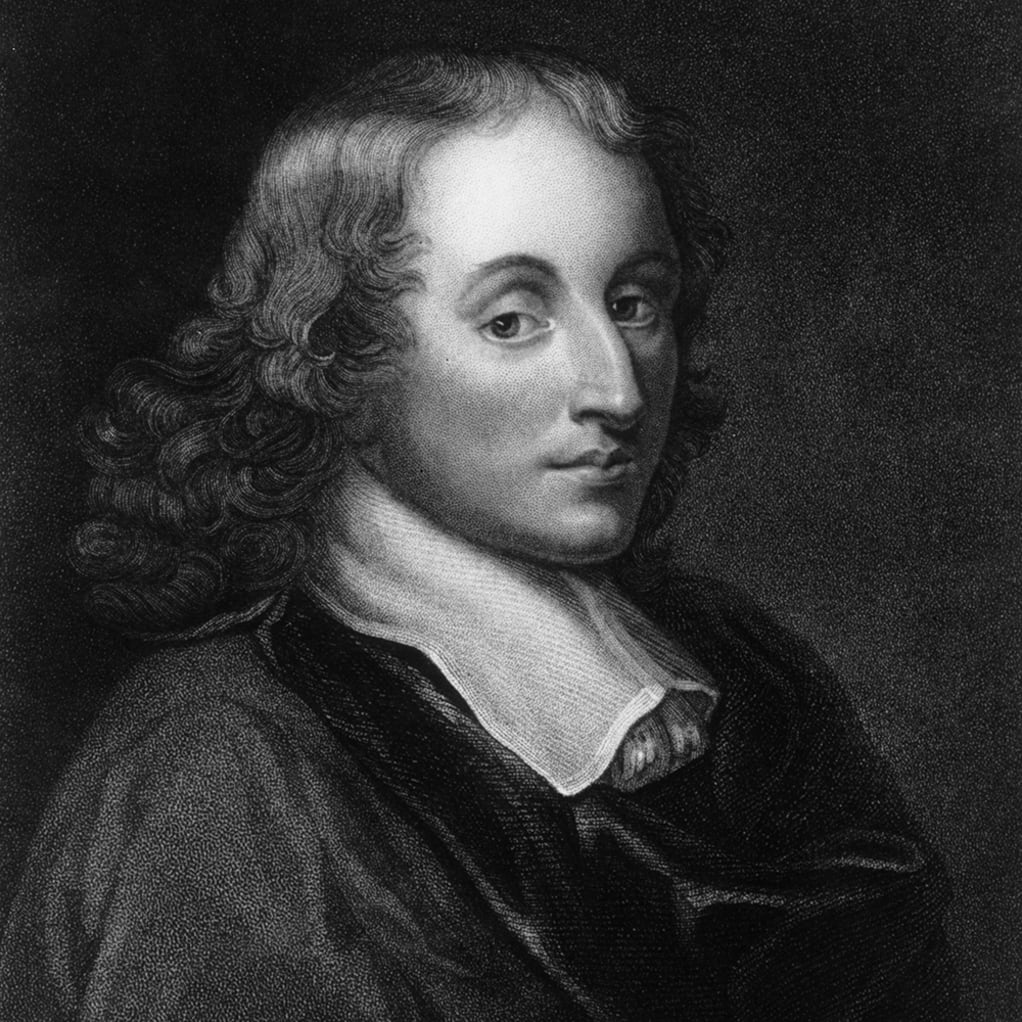
\includegraphics[width=\linewidth]{Images/ApendiceA/PASCAL.jpeg}
\textbf{Blaise Pascal:} Nacido el 19 de junio de 1623 en Clermont-Ferrand, Francia; fue un genio precoz y de clara inteligencia, pues su entusiasmo juvenil por la ciencia se materializó en importantes y precursoras aportaciones a la física y a las matemáticas. Siendo aún niño, con solo doce años, sin ayuda alguna demostró que la suma de los ángulos de un triángulo es siempre igual a 180°. Pese a su frágil salud y corta vida, murió a los treinta y nueve años, pero su huella quedó grabada en la historia de la física y de la informática.
}
\sideFigure[\label{fig:INDUCCION}Representación del Principio de Inducción]{
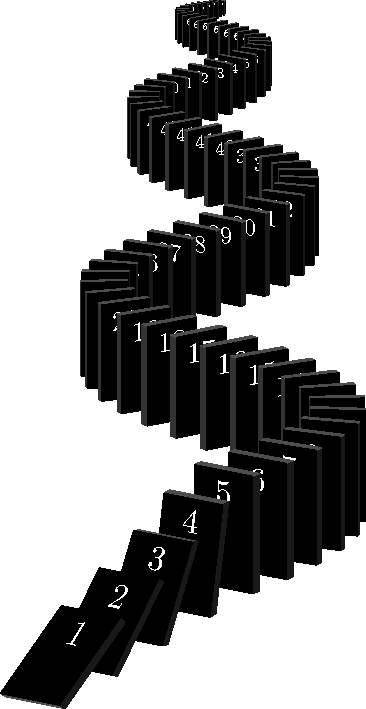
\includegraphics[width=\linewidth]{Images/ApendiceA/uuu.pdf}
}

Como preliminar, debemos saber que cualquier proposición se puede clasificar como general o particular. Algunos ejemplos de proposiciones generales son:
\begin{enumerate}
    \item Todos los ciudadanos de México tienen derecho a la educación.
    \item Todos los números que terminan en cero son divisibles entre 5.
\end{enumerate}
Algunos ejemplos de proposiciones particulares son:
\begin{enumerate}
    \item Guinevere tiene derecho a la educación 
    \item 300 es divisible entre 5.
\end{enumerate}
El proceso de obtener una proposición particular de una general se llama \textbf{deducción}. Por ejemplo, si tenemos
\begin{enumerate}
    \item Todos los ciudadanos de México tienen derecho a la educación.
    \item Guinevere es mexicana.
    \item Guinevere tiene derecho a la educación.
\end{enumerate}
entonces de la proposición general (1), junto con la proposición particular (2), se obtiene la proposición particular (3).

El proceso de obtener proposiciones generales de proposiciones particulares se llama \textbf{inducción}. El razonamiento inductivo puede conducir a conclusiones falsas así como a verdaderas. Por ejemplo, si tenemos
\begin{enumerate}
    \item 300 es divisible entre 5.
    \item Todos los números que terminan en cero son divisibles entre 5.
\end{enumerate}
entonces la proposición general (2), obtenida de la proposición particular (1), es verdadera. Pero, si consideramos
\begin{enumerate}
    \item 300 es divisible entre 5.
    \item Todos los números con tres cifras son divisibles entre 5.
\end{enumerate}
entonces la proposición general (2), deducida de la proposición particular (1), es falsa.

\begin{Problem}
    Calcular la suma de los primeros $n$ números impares. \\
    \solucion Observemos las siguientes sumas parciales:
    \begin{align*}
        1 &=1 \\
        1+3 &=4 \\
        1+3+5 &=9 \\
        1+3+5+7 &=16 \\
        1+3+5+7+9 &=25 \\
        1+3+5+7+9+11 &=36 \\
        1+3+5+7+9+11+13 &=49 \\
        1+3+5+7+9+11+13+15 &=64 \\
        1+3+5+7+9+11+13+15+17 &=81
    \end{align*}\infoBulle{Los problemas de este tipo se pueden resolver usando una fórmula probada. Pero nos interesa resolver el problema sin recurrir a tal fórmula y aplicando el método de la inducción matemática. Para hacerlo, es necesario establecer primero una hipótesis, es decir, tratar simplemente de adivinar la solución.}
    Cada suma puede representarse en la forma
    $$\alpha + \beta + \gamma + \cdots + u = S,$$
    donde $u$ representa el último sumando y $S$ la suma. Tanto $u$ como $S$ dependen del número de sumandos, al cual denominaremos con $n$. Dadas estas convenciones podemos hacer las tablas siguientes, y encontrar en la primera de ellas alguna relación entre $n$ y $u$; y en la segunda, alguna relación entre $n$ y $S$.
    \begin{table}[h!]
        \begin{minipage}{.4\textwidth}
        \centering
            \begin{tabular}{cc}
                \toprule
                $n$ & $u$ \\
                \midrule
                $1$ & $1$ \\
                $2$ & $3$ \\
                $3$ & $5$ \\
                $4$ & $7$ \\
                $5$ & $9$ \\
                $6$ & $11$ \\
                $7$ & $13$ \\
                $8$ & $15$ \\
                $9$ & $17$ \\
                \bottomrule
            \end{tabular}
        \end{minipage}
        \begin{minipage}{.4\textwidth}
        \centering
            \begin{tabular}{cc}
                \toprule
                $n$ & $S$ \\
                \midrule
                $1$ & $1$ \\
                $2$ & $4$ \\
                $3$ & $9$ \\
                $4$ & $16$ \\
                $5$ & $25$ \\
                $6$ & $36$ \\
                $7$ & $49$ \\
                $8$ & $64$ \\
                $9$ & $81$ \\
                \bottomrule
            \end{tabular}
        \end{minipage}
    \end{table}
    \marginElement{%
    Para $n=1$:
    \begin{center}
        \begin{tikzpicture}
            \filldraw (0,0) circle (0.25cm);
        \end{tikzpicture}
    \end{center}
    Para $n=2$:
    \begin{center}
        \begin{tikzpicture}
            \filldraw (0,0) circle (0.25cm);
            \filldraw (1,0) circle (0.25cm);
            \filldraw (1,1) circle (0.25cm);
            \filldraw (0,1) circle (0.25cm);
        \end{tikzpicture}
    \end{center}
    Para $n=3$:
    \begin{center}
        \begin{tikzpicture}
            \filldraw (0,0) circle (0.25cm);
            \filldraw (1,0) circle (0.25cm);
            \filldraw (1,1) circle (0.25cm);
            \filldraw (0,1) circle (0.25cm);
            \filldraw (2,0) circle (0.25cm);
            \filldraw (2,1) circle (0.25cm);
            \filldraw (2,2) circle (0.25cm);
            \filldraw (1,2) circle (0.25cm);
            \filldraw (0,2) circle (0.25cm);
        \end{tikzpicture}
    \end{center}
    Para $n=4$:
    \begin{center}
        \begin{tikzpicture}
            \filldraw (0,0) circle (0.25cm);
            \filldraw (1,0) circle (0.25cm);
            \filldraw (1,1) circle (0.25cm);
            \filldraw (0,1) circle (0.25cm);
            \filldraw (2,0) circle (0.25cm);
            \filldraw (2,1) circle (0.25cm);
            \filldraw (2,2) circle (0.25cm);
            \filldraw (1,2) circle (0.25cm);
            \filldraw (0,2) circle (0.25cm);
            \filldraw (3,0) circle (0.25cm);
            \filldraw (3,1) circle (0.25cm);
            \filldraw (3,2) circle (0.25cm);
            \filldraw (3,3) circle (0.25cm);
            \filldraw (2,3) circle (0.25cm);
            \filldraw (1,3) circle (0.25cm);
            \filldraw (0,3) circle (0.25cm);
        \end{tikzpicture}
    \end{center}
    \captionsetup*[figure]{font={footnotesize},hypcap=false}%
    \captionof{figure}{Representación del modelo $1+3+5+\cdots +(2n-1)=n^2$ cuando $n = 1$, $2$, $3$, $4$}\label{fig:JEJDJJJJJJDJJ}
    }

    \noindent Por lo que se propone el siguiente modelo:
    $$1+3+5+7+9+11+\cdots +(2n-1)=n^2.$$
    Probemosla por medio de inducción sobre $n$. Llamemos a la suma, $S_n$. Es decir,
    $$S_n=1+3+5+7+9+11+\cdots +(2n-1).$$
    \begin{enumerate}[label=\roman*.]
        \item Para $n=1$ es evidente que se cumple, ya que la suma consiste en un solo término, el $1$. El valor de la expresión $n^2$ también es $1$.
        \item Supóngase que la hipótesis se cumple para $n=k$, es decir, $S_k=k^2$.
        \item A partir de (ii), probemos que se cumple para $n=k+1$, es decir,
        $$S_{k+1}=(k+1)^2.$$
        En efecto, se tiene
        $$S_{k+1}=S_k+(2k+1)$$
        pero $S_k=k^2$, se sigue que
        $$S_{k+1}=k^2+(2k+1)=(k+1)^2$$
    \end{enumerate}
    En conclusión, se cumple que $S_n=n^2$. Incluso, para este caso, podemos ver la \emph{demostración visual} de\infoBulle{Una demostración visual implica que la solución de un problema sea accesible de manera clara a través de un diagrama o dibujo, con un mínimo de desarrollo matemático necesario.}
    $$1+3+5+7+9+11+\cdots +(2n-1)=n^2$$
    como se muestra en la figura \ref{fig:JEJDJJJJJJDJJ}. Aunque no se debe olvidar que esto es una manera visual de ver el comportamiento de una proposición particular. No siempre se puede recurrir a una demostración visual, ya que nos puede llevar a conclusiones falsas.
\end{Problem}

\section{Inducción errónea en las matemáticas}

\begin{example}
    Consideremos el polinomio $f(x)=x^2+x+41$. Si este polinomio se remplaza $x$ por el número $0$, se obtiene el número primo $41$. Si se remplaza $x$ por el número $1$, nuevamente se obtiene un número primo, $43$. Si se sigue este procedimiento para $1$, $2$, $3$, $4$, $5$, $6$; obtenemos que
    \begin{align*}
        f(0) &=41 \\
        f(1) &=43 \\
        f(2) &=47 \\
        f(3) &=53 \\
        f(4) &=61 \\
        f(5) &=71 \\
        f(6) &=83 \\
        f(7) &=97
    \end{align*}
    Basándonos en estos resultados podríamos concluir que para todo entero no negativo $x$, el valor del polinomio es un número primo. Pero esto no es así, pues el polinomio $x^2+x+41$ produce números primos para $f(0)$, $f(1)$, $f(2)$, $f(3)$, $\dots$, $f(38)$, $f(39)$ y al obtener el resultado de $f(40)$, que es $1681$, vemos que es un número compuesto.
\end{example}

\begin{example}
    El binomio $x^n-1$, $n \in \NN$, fue estudiado por numerosos matemáticos y fue resuelto en factores (con coeficientes enteros). Al estudiar dichas factorizaciones para muchos valores particulares de $n$, los matemáticos notaron que, en cada uno de los casos estudiados, los valores absolutos de los coeficientes de los factores nunca excedieron al número $1$. Es decir,
    \begin{align*}
        x-1 &=x-1 \\
        x^2-1 &=(x-1)(x+1) \\
        x^3-1 &=(x-1)\left( x^2+x+1 \right) \\
        x^4-1 &=(x-1)(x+1)\left(x^2+1\right) \\
        &\vdots 
    \end{align*}
    Se construyeron tablas de los coeficientes y, en cada uno de los casos, los coeficientes tenían la propiedad antes mencionada. Sin embargo, fallaron todos los intentos para probar que la proposición era verdadera para todos los valores de $n$. No fue hasta que V. Ivanov resolvió dicho problema en 1941. Si $n<105$, el binomio $x^n-1$ tiene la propiedad anterior. No obstante, uno de los factores de $x^{105}-1$ es el polinomio
    \begin{align*}
        x^{48} & +x^{47}+x^{46}-x^{43}-x^{42}-2x^{41}-x^{40}-x^{39}+x^{36}+x^{35}+x^{34}+x^{33} \\
        &+x^{32}+x^{31}-x^{28}-x^{26}-x^{24}-x^{22}-x^{20}+x^{17}+x^{16}+x^{15}+x^{14} \\
        &+x^{13}+x^{12}-x^9-x^8-2x^7-x^6-x^5+x^2+x+1
    \end{align*}
    que ya no tiene esta propiedad.
\end{example}

\section{El principio de la inducción matemática}

\noindent\textbf{Principio de Inducción Matemática:} Sea $P$ una propiedad cualquiera. Tenemos que $P(1), P(2), P(3), P(4), \dots$ es un conjunto de propiedades para cada número natural tal que:
\begin{enumerate}[label=\roman*.]
    \item $P(1)$ es cierta.
    \item Si $P(n)$ es cierta, entonces $P(n+1)$ es cierta.
\end{enumerate}
Entonces $P(n)$ es cierta para toda $n \in \NN$.

\begin{example}
    Demostrar que
    $$1+2+\cdots +n=\frac{n(n+1)}{2}, \forall n \in \NN.$$\newpage
    \demostracion Claramente $n=1$, satisface la fórmula, ya que
    \begin{align*}
        1 &=\frac{1(1+1)}{2} \\
        1 &=1
    \end{align*}
    lo cual es cierto. Supongamos que la fórmula se cumple para $n=k$, es decir, supongamos que
    $$1+2+\cdots +k=\frac{k(k+1)}{2}.$$
    Demostraremos a partir de lo dicho anteriormente que la fórmula se cumple para $n=k+1$. Es decir, probaremos que
    $$1+2+\cdots +k=\frac{(k+1)(k+2)}{2}.$$
    En efecto, por hipótesis de inducción
    $$1+2+\cdots +k=\frac{k(k+1)}{2}.$$
    Entonces
    \begin{align*}
        1+2+\cdots +k+k+1 &=\frac{k(k+1)}{2}+k+1 \\
        &=\frac{k(k+1)+2(k+1)}{2} \\
        &=\frac{(k+1)(k+2)}{2}
    \end{align*}
    es decir
    $$1+2+\cdots +k+1=\frac{(k+1)(k+2)}{2}.$$
    Por tanto,
    $$1+2+\cdots +n=\frac{n(n+1)}{2}, \forall n \in \NN.$$
\end{example}

\begin{example}
    Demostrar que
    $$1^3+2^3+\cdots +n^3=(1+2 +\cdots +n)^2, \forall n \in \NN.$$
    \demostracion Claramente $n=1$ satisface la fórmula, ya que al sustituir $n$ por $1$ se tiene
    \begin{align*}
        1^3 &=(1)^2 \\
        1 &=1
    \end{align*}
    lo cual es verdadero. Notemos por el ejercicio anterior que
    $$1+2+\cdots +n=\frac{n(n+1)}{2}$$
    entonces tenemos que
    $$1^3+2^3+\cdots +n^3=\left( \frac{n(n+1)}{2} \right)^2.$$
    Así pues, supongamos que la fórmula cumple para $n=k$, es decir
    $$1^3+2^3+\cdots +k^3=\left( \frac{k(k+1)}{2} \right)^2.$$\newpage\noindent
    Demostraremos a partir de lo dicho anteriormente que la fórmula se cumple para $n=k+1$. Es decir, probaremos que
    $$1^3+2^3+\cdots +k^3=\left( \frac{k(k+1)}{2} \right)^2.$$
    En efecto: por hipótesis de inducción
    \begin{align*}
        1^3 +2^3+ \cdots +k^3+(k+1)^3 &=\left( \frac{k(k+1)}{2} \right)^2 +(k+1)^3\\
        &=\frac{k^2(k+1)^2}{4}+(k+1)^3 \\
        &=\frac{k^2(k+1)^2+4(k+1)^3}{4} \\
        &=\frac{(k+1)^2\big(k^2+4(k+1)\big)}{4} \\
        &=\frac{(k+1)^2 (k^2+4k+4)}{4} \\
        &=\frac{(k+1)^2(k+2)^2}{4} \\
        &=\left(\frac{(k+1)(k+2)}{2}\right)^2
    \end{align*}
    Por tanto,
    $$1^3+2^3+\cdots +n^3=(1+2+\cdots +n)^2, \forall n \in \NN.$$
\end{example}

\begin{remark}
    El método de la inducción matemática no es el único procedimiento para demostrar que una propiedad $P$ se cumple para cada número natural.
\end{remark}

\begin{remark}
    Si no se puede demostrar que una propiedad $P$ se cumple para cada número natural, no significa que $P$ sea falsa, sino solamente que no se ha podido hacer la demostración. Una manera de demostrar que $P$ es falsa sería dar un contraejemplo.
\end{remark}

\begin{example}
    Demostrar que
    $$1^2+2^2+\cdots +n^2=\frac{n(n+1)(2n+1)}{6}, \forall n \in \NN.$$
    \demostracion Claramente $n=1$ satisface la fórmula, ya que al sustituir $n$ por $1$ se tiene
    \begin{align*}
        1^2 &=\frac{1(1+1)(2\cdot 1+1)}{6} \\
        1 &=1
    \end{align*}
    lo cual es verdadero. Supongamos que la fórmula se cumple para $n=k$, es decir, supongamos que
    $$1^2+2^2+\cdots +k^2=\frac{k(k+1)(2k+1)}{6}$$
    Demostraremos a partir de lo dicho anteriormente que la fórmula se cumple para $n=k+1$. Es decir, probaremos que
    $$1^2+2^2+\cdots +(k+1)^2=\frac{(k+1)(k+2)(2k+3)}{6}.$$
    En efecto: por hipótesis de inducción
    $$1^2+2^2+\cdots +k^2=\frac{k(k+1)(2k+1)}{6}.$$\newpage\noindent
    Entonces
    \begin{align*}
        1^2 +2^2+\cdots +k^2+(k+1)^2 &=\frac{k(k+1)(2k+1)}{6}+(k+1)^2 \\
        &=\frac{k(k+1)(2k+1)+6(k+1)^2}{6} \\
        &=\frac{(k+1)\big(k(2k+1)+6(k+1)\big)}{6} \\
        &=\frac{(k+1)(2k^2+7k+6)}{6} \\
        &=\frac{(k+1)(k+2)(2k+3)}{6}
    \end{align*}
    Por tanto,
    $$1^2+2^2+\cdots +n^2=\frac{n(n+1)(2n+1)}{6}, \forall n \in \NN.$$
\end{example}

En resumen, cuando se quiere demostrar que una propiedad $P$ se cumple para cada número natural, se emplea un procedimiento llamado \emph{demostración por inducción matemática}. Es decir, si $\NN$ es el conjunto de los números naturales y $A \subset \NN$ tal que:
\begin{enumerate}[label=\roman*.]
    \item $1 \in A$.
    \item $k \in A \Longrightarrow k+1 \in A$. Entonces $A = \NN$.
\end{enumerate}

\section{El principio de inducción modificado}

\noindent\textbf{Principio de Inducción Modificado:} Si $A$ es un subconjunto de los números naturales tal que
\begin{enumerate}[label=\roman*.]
    \item $1 \in A$.
    \item Si $1, 2, \dots , n \in A$, implica que $n+1 \in A$.
\end{enumerate}
    Entonces $A=\NN$.

\begin{observation}
    Sea $P(n)$ una propiedad cualquiera. Si se quiere demostrar que $P(n)$ es cierta para toda $n \in \NN$, es decir,
    $$A:=\left\lbrace n \in \NN \mid P(n) \text{ es cierta} \right\rbrace = \NN$$
    es suficiente mostrar que $A$ satisface las dos hipótesis del Principio de Inducción Modificado.
\end{observation}

\begin{observation}
    Podría suceder que $P(n)$ no sea verdadera para todos los números naturales, pero existe cierto número natural $i$ tal que $P(k)$ es verdadera para toda $i \leq k$. Se puede utilizar también el Principio de Inducción Modificado considerando al conjunto
    $$A:=\left\lbrace n \in \NN \mid P(n+i) \text{ es cierta} \right\rbrace $$
    en cuyo caso se reduce a demostrar que:
    \begin{enumerate}[label=\roman*.]
        \item $P(i)$ es verdadera.
        \item Si $P(k)$ es cierta para $k=i, i+1, \dots, i+n$, entonces $P\big( i+(n+1) \big)$ es cierta.
    \end{enumerate}
\end{observation}

\begin{proposition}
    El Principio de Inducción y el Principio de Inducción Modificado son equivalentes. \\
    \demostracion Se deja como ejercicio al lector.
\end{proposition}

\newpage

\section{El principio de buen orden}

\noindent\textbf{Principio del Buen Orden:} Si $A$ es un subconjunto no vacío de los números naturales, entonces $A$ posee primer elemento (o mínimo), es decir, existe $a \in A$ tal que $a \geq b$, $\forall b \in A$.

\begin{definition}
    Para toda $n \in \NN$, definimos a $S(n)=n+1$ como el sucesor de $n$.
\end{definition}

\begin{definition}
    Para toda $n \in \NN$ tal que $n \geq 1$, definimos el antecesor de $n$ como $n-1$.
\end{definition}

\begin{theorem}
    El Principio de Buen Orden es equivalente al Principio de Inducción. \\
    \demostracion Se deja como ejercicio al lector.
\end{theorem}

\section{Más ejemplos de inducción}

\begin{example}
    Demuestre que
    $$\int_{0}^{\infty} e^{-x}x^{n} dx=n!, \forall n \in \NN.$$
    \demostracion En esta demostración, tomaremos al $0$ como un número natural. Además, recordemos la siguiente propiedad
    $$\lim_{x \to \infty} e^{px}=0, \text{ si } p<0.$$
    Así pues, si $n=0$, entonces
    \begin{align*}
        \int_{0}^{\infty} e^{-x}x^0 dx &= \int_{0}^{\infty} e^{-x} dx \\
        &=\left. -e^{-x} \right|_{0}^{\infty} \\
        &=- \lim_{x \rightarrow \infty} e^{-x} + e^{-0} \\
        &=1 \\
        &=0!
    \end{align*}
    Supongamos que se cumple para $n=k$, es decir,
    $$\int_{0}^{\infty} e^{-x}x^{k} dx=k!.$$
    Demostraremos a partir lo dicho anteriormente, que la propiedad se cumple para $n=k+1$, es decir,
    $$\int_{0}^{\infty} e^{-x}x^{k+1} dx=(k+1)!.$$
    Procederemos por integración por partes. Así pues, tomando a
    $$u=x^{k+1} \quad \text{ y } \quad dv=e^{-x} dx$$
    obtenemos
    $$du=(k+1)x^k dx \quad \text{ y } \quad v=-e^{-x}$$
    Entonces
    \begin{align*}
        \int_{0}^{\infty} e^{-x}x^{k+1} dx &= \left. -x^{k+1}e^{-x} \right|_{0}^{\infty} + (k+1) \int_{0}^{\infty} e^{-x} x^k dx \\
        &=- \lim_{x \rightarrow \infty} x^{k+1}e^{-x}+(0)^{k+1}e^{-0}+(k+1)k! \\
        &=- \lim_{x \rightarrow \infty} \frac{(k+1)!}{e^x} +(k+1)k! \\
        &=(k+1)!
    \end{align*}
    Por tanto,
    $$\int_{0}^{\infty} e^{-x}x^{n} dx=n!, \forall n \in \NN.$$
\end{example}

\begin{example}
    Si $a_1, a_2, \dots, a_n$ son números reales positivos, demuestre que
    \begin{equation}
        \sqrt[n]{a_1\cdot a_2 \cdots a_n} \leq \frac{a_1+a_2+\cdots +a_n}{n}. \label{A1}
    \end{equation}
    \demostracion \sideFigure[\label{fig:JNVKJYYS}]{
    \begin{center}
        \begin{tikzpicture}[baseline=(current bounding box.north),scale=1.2]
            \begin{scope}
                \clip (-2.1,-0.01) rectangle (2.1,2.1);
                \draw[thick] (0,0) circle (2);
                \draw[thick] (-2,0) -- (2,0);
                \draw (1,0) -- (1,1.7) -- (0,0);
                \draw[stealth-stealth] (1.4,0) -- (1.4,1.73);
                \node[fill=white,rotate=90] at (1.4,0.6) {$\sqrt{a_1a_2}$};
            \end{scope}
            \draw[stealth-stealth] (-2,-0.5) -- (1,-0.5);
            \node at (-0.5,-0.5) [below] {$a_1$};
            \draw[stealth-stealth] (1,-0.5) -- (2,-0.5);
            \node at (1.5,-0.5) [below] {$a_2$};
            \draw[stealth-stealth] (-0.3,0.1) -- (0.7,1.83);
            \node[fill=white,rotate=60] at (0.1,1) {$\displaystyle \frac{a_1+a_2}{2}$};
        \end{tikzpicture}
    \end{center}
    }
    \begin{enumerate}[label=\roman*.]
        \item Para $n = 2$, la desigualdad \eqref{A1} da
        \begin{equation}
            \sqrt{a_1a_2} \leq \frac{a_1+a_2}{2}. \label{A2}
        \end{equation}
        Es fácil obtener esta desigualdad a partir de esta otra
        $$\left( \sqrt{a_1} - \sqrt{a_2} \right)^2 \geq 0,$$
        válida para cualesquiera $a_1$, $a_2$ números reales positivos. Notemos que la desigualdad \eqref{A2} admite una interpretación geométrica sencilla. Tomemos sucesivamente en una recta $AB$ los segmentos $a_1$ y $a_2$. Construyamos la circunferencia cuyo diámetro es la suma de estos segmentos. Entonces, $\displaystyle \frac{a_1+a_2}{2}$ es el radio de esta circunferencia y $\sqrt{a_1a_2}$ es la mitad de la cuerda perpendicular al diámetro en el punto común de los segmentos $a_1$ y $a_2$ (vea la figura \ref{fig:JNVKJYYS}); de aquí se deduce la desigualdad \eqref{A2}.
        \item Supongamos que la desigualdad \eqref{A1} se cumple para $n = k$. Demostremos que, entonces, también se cumple para $n = 2k$. En efecto,
        \begin{align*}
            \sqrt[2k]{a_1\cdot a_2 \cdots a_{2k}} & = \sqrt{\sqrt[k]{a_1 \cdot a_2 \cdots a_k}\sqrt[k]{a_{k+1} \cdots a_{2k}}} \\
            & \leq \frac{\sqrt[k]{a_1 \cdot a_2 \cdots a_k} + \sqrt[k]{a_{k+1} \cdots a_{2k}}}{2} \\
            & \leq \displaystyle\frac{\displaystyle\frac{a_1+a_2+\cdots +a_k}{k} +\displaystyle\frac{a_{k+1}+\cdots+a_{2k}}{k}}{2} \\
            & = \frac{a_1+a_2+\cdots+a_k+\cdots+a_{2k}}{2k}
        \end{align*}
        Puesto que hemos demostrado ya la desigualdad \eqref{A1} para $n = 2$, podemos afirmar ahora que de cumple para $n = 4$, $8$, $16$, etc., o sea, para $n = 2^s$, donde $s$ es un número natural.
        \item Para demostrar que la desigualdad \eqref{A1} se cumple para cualquiera que sea el número natural $n$, probemos que si se cumple para $n = k$, también se cumple para $n = k-1$.
        
        Sean pues, $a_1$, $a_2$, $\dots$, $a_{k-1}$ números reales positivos. Sea $\lambda$ un número real positivo, entonces
        $$\sqrt[k]{a_1 \cdot a_2 \cdots a_{k-1}\lambda} \leq \frac{a_1+a_2+\cdots+a_{k-1}+\lambda}{k}.$$
        Determinemos $\lambda$ de modo que
        $$\frac{a_1+a_2+\cdots+a_{k-1}+\lambda}{k} = \frac{a_1+a_2+\cdots+a_{k-1}}{k-1},$$
        o sea, pongamos
        $$\lambda = \frac{a_1+a_2+\cdots+a_{k-1}}{k-1}.$$\newpage
        Tenemos
        $$\sqrt[k]{\frac{a_1 \cdot a_2 \cdots a_{k-1} (a_1+a_2+\cdots+a_{k-1})}{k-1}} \leq \frac{a_1+a_2+\cdots+a_{k-1}}{k-1},$$
        es decir,
        $$\sqrt[k-1]{a_1 \cdot a_2 \cdots a_{k-1}} \leq \frac{a_1+a_2+\cdots+a_{k-1}}{k-1}.$$
        Sea ahora $m$ un número natural cualquiera. Si $m = 2^s$, la desigualdad se cumple en virtud de (ii). Si $m \neq 2^s$, determinemos el número $s$ de modo que $m$ sea menor que $2^s$; entonces, basándonos en (ii) y (iii), podemos afirmar que la desigualdad se cumple para $n = m$.
    \end{enumerate}
    Por tanto, se cumple que\infoBulle{Obsérvese que si $a_1 = a_2 = \cdots = a_n$, entonces $$\sqrt[n]{a_1\cdot a_2 \cdots a_n} = \frac{a_1+a_2+\cdots +a_n}{n}.$$En caso contrario, $$\sqrt[n]{a_1\cdot a_2 \cdots a_n} < \frac{a_1+a_2+\cdots +a_n}{n}.$$ para cualesquiera $a_1$, $a_2$, $\dots$, $a_n$ números reales positivos}
    $$\sqrt[n]{a_1\cdot a_2 \cdots a_n} \leq \frac{a_1+a_2+\cdots +a_n}{n}, \forall a_1, a_2, \dots, a_n \in \RR[+], \forall n \in \NN.$$
\end{example}

\begin{example}
    Hallar una expresión para la suma
    $$1 \cdot 1! + 2 \cdot 2! + 3 \cdot 3! + \cdots + n \cdot n!.$$
    \demostracion Llamemos a la suma anterior, $S_n$. Es decir
    $$S_n=1 \cdot 1! + 2 \cdot 2! + 3 \cdot 3! + \cdots + n \cdot n!.$$
    Veamos las siguientes sumas parciales
    \begin{align*}
        1 \cdot 1! &=1 \\
        1 \cdot 1!+2 \cdot 2! &=5 \\
        1 \cdot 1!+2 \cdot 2! + 3 \cdot 3! &=23 \\
        1 \cdot 1!+2 \cdot 2! + 3 \cdot 3! +4 \cdot 4! &=119
    \end{align*}
    Examinando las anteriores sumas, se observa que
    \begin{align*}
        S_1 &=2!-1 \\
        S_2 &=3!-1 \\
        S_3 &=4!-1 \\
        S_4 &=5!-1
    \end{align*}
    Esto conduce a la hipótesis
    $$S_n=(n+1)!-1.$$
    Verifiquemos dicha hipótesis.
    \begin{enumerate}[label=\roman*.]
        \item La hipótesis se cumple para $n=1$, pues
        $$S_1=1 \cdot 1!=2!-1.$$
        \item Supongamos que la hipótesis se cumple para $n=k$, es decir,
        $$S_k=(k+1)!-1.$$
        \item A partir de (ii), probemos que se cumple para $n=k+1$, es decir,
        $$S_{k+1}=(k+2)!-1.$$
        En efecto,
        \begin{align*}
            S_{k+1} &= S_k + (k+1) \cdot (k+1)! \\
            &=[(k+1)!-1]+(k+1) \cdot (k+1)! \\
            &=(k+1)![1+(k+1)]-1 \\
            &=(k+1)!(k+2)-1 \\
            &=(k+2)!-1
        \end{align*}
    \end{enumerate}
    Por tanto,
    $$1 \cdot 1! + 2 \cdot 2! + 3 \cdot 3! + \cdots + n \cdot n! = (n+1)!-1.$$
\end{example}

\newpage

\section{Ejercicios}

\begin{enumerate}
    \item Demostrar que
    $$1^2+3^2+\cdots +(2n-1)^2=\frac{4n^3-n}{3}, \forall n \in \NN.$$
    \item Demostrar que
    $$\frac{1}{1\cdot 2}+\frac{1}{2\cdot 3}+\frac{1}{3\cdot 4}+\cdots +\frac{1}{n(n+1)}=\frac{n}{n+1}, \forall n \in \NN.$$
    \item Demostrar que
    $$\frac{1}{1\cdot 3}+\frac{1}{3\cdot 5}+\frac{1}{5\cdot 7}+\cdots +\frac{1}{(2n-1)(2n+1)}=\frac{n}{2n+1}, \forall n \in \NN.$$
    \item Demostrar que
    $$2^n>n, \forall n \in \NN.$$
    \item Demostrar que
    $$1^2-2^2+3^2-4^2+\cdots +(-1)^{n-1}n^2=(-1)^{n-1} \frac{n(n+1)}{2}, \forall n \in \NN.$$
    \item Demostrar que para toda $n \in \NN$
    $$1 \cdot 2 \cdot 3 + 2\cdot 3 \cdot 4 + \cdots + n(n+1)(n+2) = \frac{n(n+1)(n+2)(n+3)}{4}.$$
    \item Demostrar que para toda $n \in \NN$, $n>1$
    $$\frac{1}{n+1}+\frac{1}{n+2}+\cdots +\frac{1}{2n}>\frac{13}{24}.$$
    \item Demostrar que para toda $n \in \NN$, $n>1$
    $$\frac{1}{\sqrt{1}}+\frac{1}{\sqrt{2}}+\cdots +\frac{1}{\sqrt{n}}>\sqrt{n}.$$
    \item Demostrar que para toda $n \in \NN$
    $$1+2n \leq 3^n.$$
    \item Demuestre que $(n-1)^2 \mid n^{n-1}-1$ para toda $n \in \NN$, $n>1$.
    \item Demuestre que $n^2+n$ es un número par para toda $n \in \NN$.
    \item Demuestre que $8^n-3^n$ es múltiplo de $5$ para toda $n \in \NN$.
    \item Demuestre que $n^3-n$ es múltiplo de $6$ para toda $n \in \NN$.
    \item Demuestre que $2^{2n-1}+3^{2n-1}$ es múltiplo de $5$ para toda $n \in \NN$.
    \item Demuestre que $11^{n+1}+12^{2n-1}$ es múltiplo de $19$ para toda $n \in \NN$.
    \item Si $a \neq 1$, entonces
    $$1+a+a^2+\cdots +a^n=\frac{a^{n+1}-1}{a-1}, \forall n \in \NN.$$
    \item Demuestre que
    $$3+3^2+3^3+\cdots +3^n=\frac{3(3^n-1)}{2}, \forall \in \NN.$$\newpage
    \item Demostrar por inducción
    $$1+nx \leq (1+x)^n, \forall n \in \NN, x \geq -1.$$
    Esta desigualdad es conocida como desigualdad de Bernoulli.
    \item Demuestre que el número $S_n$ de permutaciones de $n$ elementos está dado por
    $$S_n=n!.$$
    \item Demuestre que si $a \neq b$, entonces el siguiente determinante de $n \times n$ se cumple:
    $$
    \begin{vmatrix}
        a+b & ab & 0 & \cdots & 0 & 0 \\
        1 & a+b & ab & \cdots & 0 & 0 \\
        0 & 1 & a+b & \ddots & 0 & 0 \\
        \vdots & & & \ddots & \\
        0 & 0 & 0 & \ddots & a+b & ab \\
        0 & 0 & 0 & \cdots & 1 & a+b
    \end{vmatrix} = \frac{a^{n+1}-b^{n+1}}{a-b}.
    $$
    \item Probar la identidad
    $$\cos (\varphi) \cos (2\varphi) \cos (4\varphi) \cdots \cos \left( 2^n \varphi \right)=\frac{\sen \left( 2^{n+1} \varphi \right)}{2^{n+1} \sen (\varphi)}.$$
    \item Probar que
    $$\frac{1}{2}+\cos x +\cos 2x +\cdots +\cos nx=\frac{ \sen \frac{2n+1}{2}x}{2\sen \frac{x}{2}}.$$
    \item Demuestre que
    $$\frac{d^n}{dx^n}\left( \frac{\sen x}{x} \right) = \frac{1}{x^{n+1}} \int_{0}^{x} y^n \cos \left( y+\frac{n\pi}{2} \right) dy, \forall n \in \NN.$$
    \item Demuestre que
    $$\binom{n}{0}+\binom{n}{1}+\cdots +\binom{n}{n}=2^n, \forall n \in \NN.$$
    \item Sea $n$, $k \in \NN$ con $0 \leq k \leq n$, demuestre que
    $$\binom{k}{k}+\binom{k+1}{k}+\binom{k+2}{k}+\cdots +\binom{n}{k}=\binom{n+1}{k+1}.$$
\end{enumerate}

\chapter{NÚMEROS COMPLEJOS}\label{chap:numeros-complejos}
\printchaptertableofcontents

\section{El conjunto de los números complejos}

Los números complejos son una extensión del conjunto de los números reales. A medida que exploramos las complejidades del álgebra, nos encontramos con esta rama que añade una nueva dimensión a nuestro entendimiento numérico. La unidad imaginaria, denotada como $i$, desempeña un papel central en este contexto, ya que nos lleva más allá de las limitaciones de los números reales.

En el siglo XVI, los matemáticos se enfrentaron al problema de encontrar soluciones a ecuaciones cuadráticas que involucraban raíces cuadradas negativas. Por ejemplo, la ecuación \(x^2 + 1 = 0\) no tiene soluciones en los números reales, ya que no hay ningún número real cuyo cuadrado sea $-1$.

La historia de los números complejos es rica y tiene sus raíces en la necesidad de encontrar soluciones a ecuaciones aparentemente insolubles en el ámbito de los números reales. El concepto de números complejos se desarrolló a lo largo de varios siglos, con contribuciones significativas de matemáticos de diversas culturas. Aquí se mencionan algunas:
\begin{itemize}
    \item Cardano y la fórmula Cubica: En el siglo XVI, el matemático italiano Gerolamo Cardano desarrolló la fórmula para encontrar soluciones a ecuaciones cúbicas. Esta fórmula implicaba tomar raíces cuadradas de números negativos, aunque Cardano mismo no comprendía completamente las implicaciones de este proceso. En el \hyperref[sec:radical]{Apéndice D} se habla más detalladamente sobre la historia de la ecuación de segundo y tercer grado.
    \item Bombelli y la aceptación de lo “imaginario”: Rafael Bombelli, a finales del siglo XVI, fue uno de los primeros en tratar con números imaginarios de manera sistemática. En su obra “L'Algebra”, introdujo términos imaginarios para representar las raíces cuadradas de números negativos. Aunque no siempre entendía completamente la naturaleza de estos números, los utilizaba de manera efectiva.
    \item Descartes y la coordenada compleja: En el siglo XVII, René Descartes introdujo la representación geométrica de números complejos en un plano bidimensional, asociando la parte real con el eje horizontal y la parte imaginaria con el eje vertical. Esta representación facilitó la visualización de las operaciones con números complejos.
    \item Euler y la identidad Exponencial: En el siglo XVIII, Leonhard Euler desempeñó un papel crucial al establecer la forma polar de los números complejos y la famosa identidad de Euler
    \[e^{i\theta} = \cos(\theta) + i\sin(\theta).\]
    Esto unificó las representaciones rectangular y polar de los números complejos, proporcionando una herramienta poderosa para manipularlos.
\end{itemize}

En resumen, la historia de los números complejos es una narrativa fascinante que involucra la superación de obstáculos conceptuales y la evolución de la comprensión matemática. Desde sus raíces en la resolución de ecuaciones cuadráticas hasta su papel central en la física teórica moderna, los números complejos han demostrado ser una herramienta poderosa y versátil en el arsenal matemático.

\begin{definition}\label{definicion:definiciondecomplejo}
    Un número complejo $z$ es una pareja ordenada de $\RR$. El conjunto de números complejos lo denotaremos por $\CC$, donde
    $$\CC=\left\{ (a,  b) \mid a,  b \in \RR \right\} .$$
\end{definition}

\begin{definition}
    Sean $z$, $w \in \CC$, con $z=(a,  b)$ y $w=(c,  d)$. Decimos que dos números complejos $z$ y $w$ son iguales, y escribiremos $z=w$, si $a=c$ y $b=d$.
\end{definition}

\begin{definition}
    Sea $z \in \CC$, con $z=a+bi$. Definimos:
    \begin{enumerate}[label=\roman*.]
        \item La parte real de $z$, denotada por $\operatorname{Re}  (z)$, como $\operatorname{Re} (z)=a$.
        \item La parte imaginaria de $z$, denotada por $\operatorname{Im} (z)$, como $\operatorname{Im} (z)=b$.
    \end{enumerate}
\end{definition}

\section{Operaciones con números complejos}

El conjunto de los números complejos se caracteriza por la presencia de dos operaciones fundamentales: la suma y el producto. Para definir la suma de dos números complejos $z$ y $w$, representados como $z=(a,  b)$ y $w=(c,  d)$ en el conjunto $\CC$, utilizamos la siguiente expresión:
$$z + w=(a,  b)+(c,  d)=(a+c,  b+d).$$
Asimismo, para definir el producto de estos números complejos $z$ y $w$, expresados como $z=(a,  b)$ y $w=(c,  d)$ en el conjunto $\CC$, empleamos la siguiente fórmula:
$$zw=(a,  b)(c,  d)=(ac-bd,  ad+bc).$$
Es importante destacar que la suma cumple con las siguientes propiedades:\newpage
\begin{enumerate}[label=A\arabic*.]
    \item Cerradura: Si $z$, $w \in \CC$, entonces $z+w \in \CC$. En efecto: Sean $z$, $w \in \CC$ con $z=(a,  b)$ y $w=(c,  d)$, entonces
    \begin{align*}
        z+w & = (a,  b)+(c,  d) \\
        & = (a+c,  b+d) \in \CC.
    \end{align*}
    \item Asociatividad: Si $z$, $w$, $y \in \CC$, entonces
    $$(z+w)+y=z+(w+y).$$
    En efecto: Sean $z$, $w \in \CC$ con $z=(a,  b)$, $w=(c,  d)$ e $y=(e,  f)$. Entonces
    \begin{align*}
        (z+w)+y &=\{(a,  b)+(c,  d) \} +(c,  f) \\
        &=(a+c,  b+d)+(e,  f) \\
        &=\big( (a+c)+e,  (b+d)+f \big) \\
        &=\big( a+(c+e),  b+(d+f) \big) \\
        &=(a,  b)+(c+e,  d+f) \\
        &=(a,  b)+ \big( (c,  d)+(e,  f) \big) \\
        &=z+(w+y).
    \end{align*}
    \item Conmutatividad: Si $z$, $w \in \CC$, entonces
    $$z+w=w+z.$$
    En efecto: Sean $z$, $w \in \CC$ tal que $z=(a,  b)$ y $w=(c,  d)$, entonces
    \begin{align*}
        z+w &=(a,  b)+(c,  d) \\
        &=(a+c,  b+d) \\
        &=(c+a,  d+b) \\
        &=(c,  d)+(a,  b) \\
        &=w+z.
    \end{align*}
    \item Elemento neutro: Existe un único número complejo, denotado por $0$, que satisface
    $$z+0=z, \; \forall z \in \CC.$$
    En efecto: Sea $z \in \CC$, con $z=(a,  b)$.
    
    \textbf{Existencia:} Sea $w=(0,  0)$, entonces
    \begin{align*}
        z+w & = (a,  b)+(0,  0) \\
        & = (a+0,  b+0) \\
        & = (a,  b) \\
        & = z.
    \end{align*}
    Por lo que $z+w=z$
    
    \textbf{Unicidad:} Sea $v \in \CC$ tal que
    $$z+v=z, \; \forall z \in \CC,$$
    en particular $z=w$, tenemos que $w+v=w$. Pero $z+w=z$, $\forall z \in \CC$, en particular para $z=v$, tenemos $v+w=v$. Así que
    \begin{align*}
        v & = v+w \\
        & = w+v \\
        & = w.
    \end{align*}
    Por lo tanto $v=w$.\newpage
    \item Inverso aditivo: Dado $z \in \CC$, existe un único número complejo, denotado por $-z$ que satisface
    $$z+(-z)=0.$$
    En efecto: Sea $z \in \CC$, con $z=(a,  b)$.
    
    \textbf{Existencia:} Sea $w=(-a,  -b)$, entonces
    \begin{align*}
        z+w &=(a,  b)+(-a,  -b) \\
        &=\big( a+(-a),  b+(-b) \big) \\
        &=(0,  0) \\
        & = 0.
    \end{align*}
    \textbf{Unicidad:} Sea $v \in \CC$ tal que $z+v=0$. Tenemos
    \begin{align*}
        w &=w+0 \\
        &=w+(z+v) \\
        &=(w+z)+v \\
        &=0+v \\
        &=v.
    \end{align*}
    Por lo tanto $w=v$.
\end{enumerate}
El producto satisface:
\begin{enumerate}[resume,label=A\arabic*.]
    \item Cerradura: Sea $z$, $w \in \CC$, entonces $zw \in \CC$. En efecto: Sea $z$, $w \in \CC$ con $z=(a,  b)$ y $w=(c, \ d)$, entonces
    \begin{align*}
        zw & = (a,  b) (c,  d) \\
        & = (ac-bd,  ad+bc) \in \CC.
    \end{align*}
    \item Asociatividad: Si $z$, $w$, $y \in \CC$, entonces
    $$(zw)y=z(wy).$$
    En efecto: Sean $z$, $w$, $y \in \CC$ con $z=(a,  b)$, $w=(c,  d)$ e $y=(e,  f)$. Entonces
    \begin{align*}
        (zw)y &=\{ (a,  b)(c,  d) \} (e,  f) \\
        &=(ac-bd,  ad+bc)(e,  f) \\
        &=\big( (ac-bd)(e)-(ad+bc)(f),  (ac-bd)(f)+(ad+bc)(e) \big) \\
        &=(ace-bde-adf-bcf,  acf-bdf+ade+bce) \\
        &=(ace-adf-bcf-bde,  acf+ade+bce-bdf) \\
        &=\big( a(ce-df)-b(cf+de),  a(cf+de)+b(ce-df) \big) \\
        &=(a,  b)(ce-df,  cf+de) \\
        &=(a,  b)\big( (c,  d)(e,  f) \big) \\
        &=z(wy).
    \end{align*}
    \item Conmutatividad: Si $z$, $w \in \CC$. Entonces
    $$zw=wz.$$
    En efecto: Sean $z$, $w \in \CC$ con $z=(a,  b)$ y $w=(c,  d)$, entonces
    \begin{align*}
        zw &=(a,  b)(c,  d) \\
        &=(ac-bd,  ad+bc) \\
        &=(ca-db,  cb+da) \\
        &=(c,  d)(a,  b) \\
        &=wz.
    \end{align*}
    \item Elemento identidad: Existe un único complejo, denotado por 1 que satisface
    $$1 \cdot z=z, \; \forall z \in \CC.$$
    En efecto: Sea $z \in \CC$ con $z=(a,  b)$.
    
    \textbf{Existencia:} Sea $w=(1,  0)$, entonces
    \begin{align*}
        wz & = (1,  0)(a,  b) \\
        & = (1a-0b,  1b+0a) \\
        & = (a,  b) \\
        & = z.
    \end{align*}
    
    \textbf{Unicidad:} Sea $v \in \CC$ tal que
    $$vz=z, \; \forall z \in \CC,$$
    en particular para $z=w$, entonces $vw=w$. Como $wz=z$, $\forall z \in \CC$, en particular $z=v$, entonces $wv=v$. Así que
    \begin{align*}
        v & = wv \\
        & = vw \\
        & = w.
    \end{align*}
    Por tanto, $v=w$.
    \item Inverso multiplicativo: Dado $z \in \CC$, con $z \neq 0$, existe un único complejo tal que
    $$z \cdot z^{-1}=1.$$
    En efecto: Sea $z \in \CC$, con $z=(a,  b)$ y $z \neq 0$, entonces $a \neq 0$ o $b \neq 0$. Deseamos encontrar $w \in \CC$ tal que $zw=(1,  0)$. Expresemos $w=(x,  y)$, entonces
    \begin{align*}
        (1,  0) &=zw \\
        &=(a,  b)(x,  y) \\
        &=(ax-by,  ay+bx).
    \end{align*}
    Luego $ax-by=1$ y $ay+bx=0$. Es decir
    $$\left\{ \begin{array}{rl}
        ax-by= & \!\!\!\! 1 \\
        ay+bx= & \!\!\!\! 0
    \end{array}\right.$$
    \begin{enumerate}[label=\roman*.]
        \item Si $a=0$, entonces $b \neq 0$. Luego $by=1$, así que $\displaystyle y=-\frac{1}{b}$, entonces $bx=0$, así que $x=0$.
        \item Si $b=0$, entonces $a \neq 0$. Luego $ax=1$, así que $\displaystyle x=\frac{1}{a}$, entonces $ay=0$, entonces $y=0$.
        \item Supongamos que $a$, $b \neq 0$. Entonces $a^2+b^2 \neq 0$, luego
        $$\begin{array}{rl}
            a^2x-aby= & \!\!\!\! a \\
            aby+b^2x= & \!\!\!\! 0
        \end{array} = \begin{array}{rl}
            a^2x-aby= & \!\!\!\! a \\
            b^2x+aby= & \!\!\!\! 0
        \end{array} \Longrightarrow x \left(a^2+b^2 \right)= a$$
        Por lo tanto, $\displaystyle x=\frac{a}{a^2+b^2}$. Por otro lado
        $$\begin{array}{rl}
            -bax+b^2y= & \!\!\!\! -b \\
            a^2y+abx= & \!\!\!\! 0
        \end{array} =
        \begin{array}{rl}
            -bax+b^2y= & \!\!\!\! -b \\
            bax+a^2y= & \!\!\!\! 0
        \end{array} \Longrightarrow y \left( a^2+b^2 \right)=-b$$
        Por lo tanto, $\displaystyle y=-\frac{b}{a^2+b^2}$. Por tanto, $\displaystyle z^{-1}=\left( \frac{a}{a^2+b^2},  \frac{-b}{a^2+b^2} \right)$.
    \end{enumerate}
\end{enumerate}\newpage
La adición y el producto se relacionan con la siguiente propiedad:
\begin{enumerate}[resume,label=A\arabic*.]
    \item Distributividad: Sean $z$, $w$, $y \in \CC$, entonces
    $$z(x+y) = zx + zy.$$
    En efecto: Se deja como ejercicio al lector.
\end{enumerate}

\begin{observation}
    Sea $X=\{(a,  0) \mid a \in \RR \}$. Sea $f: \RR \longrightarrow X$ dada por $f(a)=(a,  0)$, para todo $a \in \RR$. Sean $a,  b \in \RR$. Entonces
    \begin{align*}
        f(a+b) &=(a+b,  0) \\
        & =(a,  0)+(b,  0) \\
        &=f(a)+f(b),
    \end{align*}
    y
    \begin{align*}
        f(a) f(b) &=(a,  0)(b,  0) \\
        & =(a b - 0 \cdot 0,  a \cdot 0 + 0 \cdot b) \\
        & =(a b,  0) \\
        & =f(a b).
    \end{align*}
    \begin{enumerate}[label=\roman*.]
        \item Para demostrar que $f$ es una función inyectiva, consideremos $a, b \in \RR$ tal que $f(a)=f(b)$. Esto implica que $(a,  0)=(b,  0)$, lo que a su vez conduce a $a=b$. Por lo tanto, concluimos que $f$ es inyectiva.
        \item Para demostrar la sobreyectividad de $f$, tomemos $(a, 0) \in X$. Entonces, se cumple que $f(a)=(a,  0)$.
        \item Dado que hemos demostrado tanto la inyectividad como la sobreyectividad de $f$, podemos concluir que $f$ es una función biyectiva.
    \end{enumerate}
    Basándonos en lo expuesto anteriormente, podemos afirmar que $X$ es isomorfo al conjunto de los números reales, representado como $\RR$. Esto implica que si consideramos un elemento $a$ perteneciente a los números reales, podemos asociarlo con $(a,  0)$. De manera abreviada y abusando de la notación, podemos expresar $a=(a,  0)$. Por lo tanto, podemos establecer las siguientes identidades:
    $$1=(1,  0) \quad \text{ y } \quad 0=(0,  0).$$
\end{observation}

\begin{observation}
    Tomemos $i=(0,1)$. Observemos que
    \begin{align*}
        i^2 &=(0,  1)(0,  1) \\
        &=\big( 0(0)-1(1),  0(1)+1(0)\big)\\
        &=(-1,  0)\\
        &=-1.
    \end{align*}
    Además si $b \in \RR$, entonces
    \begin{align*}
        b i & =(b,  0)(0,  1) \\
        & =(b \cdot 0-0 \cdot 1,  b \cdot 1+0 \cdot 0) \\
        & =(0,  b).
    \end{align*}
    Por lo tanto, si $z \in \CC$, con $z=(a,  b)$, entonces:\infoBulle{A la expresión $a+bi$ se le llama forma binómica donde $a$ es la parte real y $b$ es la parte imaginaria. Esta notación facilita la manipulación algebraica de los números complejos.}
    \begin{align*}
        z &=(a,  b) \\
        & =(a,  0)+(0,  b) \\
        & =(a, 0)+(b, 0)(0,1) \\
        & =a+b i.
    \end{align*}
\end{observation}

\newpage

\begin{observation}
    Sean $z$, $w \in \CC$ con $z=a+bi$ y $w=c+di$, entonces
    \begin{align*}
        z+w &=(a+bi)+(c+di) \\
        &=(a+c)+(bi+di) \\
        &=(a+c)+(b+d)i,
    \end{align*}
    y
    \begin{align*}
        zw &=(a+bi)(c+di) \\
        &=ac+adi+bci+bidi \\
        &=ac+(ad+bc)i-bd \\
        &=(ac-bd)+(ad+bc)i.
    \end{align*}
    Si $w \neq 0$
    \begin{align*}
        w^{-1} &=\frac{1}{w} \\
        &=\frac{1}{c+di} \\
        &=\frac{1}{c+di} \cdot \frac{c-di}{c-di} \\
        &=\frac{c-di}{(c+di)(c-di)} \\
        &=\frac{c}{c^2+d^2} - \frac{d}{c^2+d^2} i.
    \end{align*}
    Por tanto, $\displaystyle w^{-1}=\frac{c}{c^2+d^2} - \frac{d}{c^2+d^2} i$.
\end{observation}

\begin{definition}
    Sean $z$, $w \in \CC$, definimos
    \begin{enumerate}[label=\roman*.]
        \item $z-w=z+(-w)$.
        \item $\displaystyle \frac{z}{w}=zw^{-1}$, con $w \neq 0$.
    \end{enumerate}
\end{definition}

\begin{observation}
    Sean $z$, $w \in \CC$ con $z=a+bi$ y $w=c+di$, entonces
    \begin{align*}
        z-w &=(a+bi)-(c+di) \\
        &=(a-c)+(b-d)i.
    \end{align*}
    Si $w \neq 0$, entonces
    \begin{align*}
        \frac{z}{w} &= \frac{a+bi}{c+di} \\
        &= \frac{a+bi}{c+di} \cdot \frac{c-di}{c-di} \\
        &= \frac{ac+bd+(-ad+cb)i}{c^2+d^2} \\
        & =\frac{ac+bd}{c^2+d^2} + \frac{-ad+cb}{c^2+d^2} i.
    \end{align*}
\end{observation}

\begin{proposition}
    Sean $z$, $z_1$, $z_2$, $z_3 \in \CC$, entonces
    \begin{enumerate}[label=\roman*.]
        \item $z \cdot 0=0$.
        \item $-z=(-1)z$.
        \item $-(-z)=z$.
        \item $(-z_1)(z_2)=z_1(-z_2)=-(z_1z_2)$.
        \item $(-z_1)(-z_2)=z_1z_2$.
        \item $z_1(z_2-z_3)=z_1z_2-z_1z_3$.
    \end{enumerate}
    \demostracion Se dejan como ejercicio al lector.
\end{proposition}

\section{El conjugado de un número complejo}

\begin{definition}
    Sea $z \in \CC$, con $z=a+bi$. Definimos el conjugado de $z$, denotado por $\overline{z}$, como $\overline{z} =a-bi$.
\end{definition}

\begin{proposition}
    Sea $z \in \mathbb{Z}$. Entonces $z \in \RR$ si y solo si $\overline{z}=z$. \\
    \demostracion Expresemos $z=a+bi$. Supongamos que $z \in \RR$, entonces $z=a+0i$, luego
    \begin{align*}
        \overline{z} &=a-0i \\
        & = a \\
        & = z.
    \end{align*}
    Por lo tanto $\overline{z}=z$. Supongamos que $\overline{z}=z$, entonces $a-bi=a+bi$, luego $a=a$ y $-b=b$, así que $b=0$ y por lo tanto $z=a \in \RR$.
\end{proposition}

\begin{proposition}
    Si $z$, $w \in \CC$, entonces $\overline{z+w}=\overline{z} +\overline{w}$. \\
    \demostracion Sean $z=a+bi$ y $w=c+di$, con $z$, $w \in \CC$, entonces $z+w=(a+c)+(b+d)i$, así pues
    \begin{align*}
        \overline{z+w} & =(a+c)-(b+d)i \\
        &=a+c-bi-di \\
        &=(a-bi)+(c-di) \\
        &=\overline{z} + \overline{w}.
    \end{align*}
    Por lo tanto $\overline{z+w}=\overline{z} + \overline{w}$.
\end{proposition}

\begin{proposition}
    Si $z \in \CC$, entonces $\overline{-z}=- \overline{z}$. \\
    \demostracion Sea $z \in \CC$ tal que $z=a+bi$, entonces $-z=-a-bi$, luego
    \begin{align*}
        \overline{-z} &=-a+bi \\
        & =-(a-bi) \\
        & =- \overline{z}.
    \end{align*}
    Por tanto, $\overline{-z}=- \overline{z}$.
\end{proposition}

\begin{proposition}
    Si $z$, $w \in \CC$, entonces $\overline{z-w}=\overline{z} - \overline{w}$. \\
    \demostracion Sean $z$, $w \in \CC$ tal que $z=a+bi$ y $w=c+di$, entonces
    \begin{align*}
        \overline{z-w} &=\overline{z+(-w)} \\
        &=\overline{z} + \overline{(-w)} \\
        &=\overline{z} + (- \overline{w}) \\
        &=\overline{z} - \overline{w}.
    \end{align*}
    Por tanto, $\overline{z-w}=\overline{z} - \overline{w}$.
\end{proposition}

\begin{proposition}
    Si $z$, $w \in \CC$, entonces $\overline{zw}=\overline{z} \cdot \overline{w}$. \\
    \demostracion Sean $z$, $w \in \CC$ tal que $z=a+bi$ y $w=c+di$, entonces $\overline{z}=a-bi$ y $\overline{w}=c-di$. Así pues
    \begin{align*}
        z \cdot w &=(ac-bd)+(ad+bc)i \\
        \overline{z \cdot w} &=(ac-bd)-(as+bc)i,
    \end{align*}
    en consecuencia
    \begin{align*}
        \overline{z} \cdot \overline{w} &=(a-bi)(c-di) \\
        &=\big( ac-(-b)(-d) \big) +\big( a(-d)+(-b)c \big) i \\
        &=(ac-bd)+(-ad-bc)i \\
        &=(ac-bd)-(ad+bc)i.
    \end{align*}
    Por lo tanto, $\overline{zw}=\overline{z} \cdot \overline{w}$.
\end{proposition}

\begin{proposition}
    Si $z \in \CC$, con $z \neq 0$, entonces $\overline{z^{-1}}=\left( \overline{z} \right)^{-1}$. \\
    \demostracion Sabemos que $z \cdot z^{-1}=1$, entonces
    \begin{align*}
        1 &=\overline{1} \\
        & =\overline{z \cdot z^{-1}} \\
        & =\overline{z} \cdot \overline{z^{-1}},
    \end{align*}
    por lo tanto $\overline{z^{-1}}=\left( \overline{z} \right)^{-1}$.
\end{proposition}

\begin{proposition}
    Si $z$, $w \in \CC$, con $w \neq 0$, entonces $\displaystyle \overline{\left( \frac{z}{w} \right)}=\frac{\overline{z}}{\overline{w}}$. \\
    \demostracion Sean $z$, $w \in \CC$, con $w \neq 0$. Entonces
    \begin{align*}
        \overline{\left( \frac{z}{w} \right)} &= \overline{z \cdot w^{-1}} \\
        & =\overline{z} \cdot \overline{w^{-1}} \\
        & =\overline{z} (\overline{w})^{-1} \\
        & =\frac{\overline{z}}{\overline{w}}.
    \end{align*}
    Por lo tanto, $\displaystyle \overline{\left( \frac{z}{w} \right)}=\frac{\overline{z}}{\overline{w}}$.
\end{proposition}

\begin{proposition}
    Si $z \in \CC$, entonces $z+\overline{z}= 2  \operatorname{Re}(z)$. \\
    \demostracion Sea $z \in \CC$ tal que $z=a+bi$, entonces
    \begin{align*}
        z+\overline{z} &=(a+bi)+(a-bi) \\
        & =2a \\
        & =2  \operatorname{Re}(z).
    \end{align*}
    Por lo tanto, $z+\overline{z}= 2  \operatorname{Re}(z)$.
\end{proposition}

\begin{proposition}
    Si $z \in \CC$, entonces $z-\overline{z}= 2  \operatorname{Im}(z)  i$. \\
    \demostracion Sea $z \in \CC$ tal que $z=a+bi$, entonces
    \begin{align*}
        z-\overline{z} &=(a+bi)-(a-bi) \\
        & =2bi \\
        & =2  \operatorname{Im}(z)  i
    \end{align*}
    Por tanto, $z-\overline{z}= 2  \operatorname{Im}(z)  i$.
\end{proposition}

\begin{proposition}
    Si $z \in \CC$, entonces $\overline{\overline{z}}=z$. \\
    \demostracion Sea $z \in \CC$ con $z=a+bi$, entonces $\overline{z}=a-bi$ y $\overline{\overline{z}}=a+bi$. Por tanto, $ \overline{\overline{z}}=z$.
\end{proposition}

\section{El módulo de un número complejo}

\begin{definition}
    Sea $z=a+bi$ un número complejo, definimos el módulo (o también conocido como valor absoluto), denotado por $|z|$, como la raíz cuadrada del número real $a^2+b^2$, es decir,
    $$|z|=\sqrt{a^2+b^2}.$$
\end{definition}

\begin{proposition}
    Si $z \in \CC$, entonces
    \begin{enumerate}[label=\roman*.]
        \item $|z| \geq 0$.
        \item $|\overline{z}|=|z|$.
        \item $|z|=0$ si y solo si $z=0$.
        \item $|z|^2=z \overline{z}$.
    \end{enumerate}
    \demostracion
    \begin{enumerate}[label=\roman*.]
        \item Sea $z \in \CC$, con $z=a+bi$, entonces
        $$a^2+b^2 \geq 0.$$
        Luego $|z|=\sqrt{a^2+b^2} \geq 0$.
        \item Sea $z \in \CC$, con $z=a+bi$, tenemos
        \begin{align*}
            |\overline{z}| &=|a-bi| \\
            &=\sqrt{a^2+(-b)^2} \\
            &=\sqrt{a^2+b^2} \\
            &=|z|.
        \end{align*}
        Por lo tanto, $|\overline{z}|=|z|$.
        \item Sea $z \in \CC$, con $z=a+bi$, entonces
        \begin{align*}
            |z|=0 & \Longleftrightarrow \sqrt{a^2+b^2}=0 \\
            & \Longleftrightarrow a^2+b^2=0 \\
            & \Longleftrightarrow a^2=0 \text{ y }  b^2=0 \\
            & \Longleftrightarrow a=0 \text{ y }  b=0 \\
            & \Longleftrightarrow z=0.
        \end{align*}
        \item Sea $z \in \CC$, con $z=a+bi$, entonces
        \begin{align*}
            z \overline{z} & = (a+bi)(a-bi) \\
            & = a^2 - (bi)^2 \\
            & = a^2 + b^2 \\
            & = \left| a^2 + b^2 \right| \\
            & = \sqrt{\left(a^2+b^2\right)^2} \\
            & = \left(\sqrt{a^2+b^2}\right)^2 \\
            & = |z|^2.
        \end{align*}
    \end{enumerate}
\end{proposition}

\begin{theorem}
    Si $z$, $w \in \CC$, entonces $|zw|=|z||w|$. \\
    \demostracion Sea $z \in \CC$, con $z=a+bi$. Entonces
    \begin{align*}
        |zw|^2 &=(zw)\left( \overline{zw} \right) \\
        &=(zw)(\overline{z} \overline{w}) \\
        &=(z \overline{z})(w \overline{w}) \\
        &=|z|^2 |w|^2 \\
        &=(|z| |w|)^2.
    \end{align*}
    Luego $\sqrt{|zw|^2}=\sqrt{(|z| |w|)^2}$, así que
    $$\big| |zw| \big| =\big| |z| |w| \big|.$$
    Por lo tanto,
    $$|zw|=|z| |w|.$$
\end{theorem}

\newpage

\begin{proposition}
    Si $z \in \CC$, con $z \neq 0$, entonces $\left| z^{-1} \right| =|z|^{-1}$. \\
    \demostracion Tenemos que $z \cdot z^{-1}=1$. Luego
    \begin{align*}
        1 &=|1| \\
        &=\left| z \cdot z^{-1} \right| \\
        &=|z| \left| z^{-1} \right|.
    \end{align*}
    Así que
    $$|z| \left| z^{-1} \right| = 1.$$
    Por lo tanto
    $$|z|^{-1}=\left| z^{-1} \right|.$$
\end{proposition}

\begin{proposition}
    Si $z$, $w \in \CC$, con $w \neq 0$, entonces $\displaystyle \left| \frac{z}{w} \right| =\frac{|z|}{|w|}$. \\
    \demostracion Tenemos
    \begin{align*}
        \left| \frac{z}{w} \right| =\left| z \cdot w^{-1} \right|  &=|z| \left| w^{-1} \right| \\
        &=|z| \left| w \right| ^{-1} \\
        &=\frac{|z|}{|w|}.
    \end{align*}
    Por lo tanto,
    $$\left| \frac{z}{w} \right| =\frac{|z|}{|w|}.$$
\end{proposition}

\begin{proposition}
    Si $z \in \CC$, entonces
    \begin{enumerate}[label=\roman*.]
        \item $\operatorname{Re}(z) \leq |z|$. 
        \item $\operatorname{Im}(z) \leq |z|$.
    \end{enumerate}
    \demostracion Sea $z \in \CC$, con $z=a+bi$
    \begin{enumerate}[label=\roman*.]
        \item Como $b^2 \geq 0$, entonces $a^2+b^2 \geq a^2$, luego $\sqrt{a^2+b^2} \geq \sqrt{a^2}$, por lo que
        \begin{align*}
            |z| &= \sqrt{a^2+b^2} \\
            & \geq \sqrt{a^2} \\
            & =|a| \\
            & \geq a \\
            & =\operatorname{Re}(z).
        \end{align*}
        \item Como $a^2 \geq 0$, entonces $a^2+b^2 \geq b^2$, luego $\sqrt{a^2+b^2} \geq \sqrt{b^2}$, por lo que
        \begin{align*}
            |z| &= \sqrt{a^2+b^2} \\
            & \geq \sqrt{b^2} \\
            & =|b| \\
            & \geq b \\
            & =\operatorname{Im}(z).
        \end{align*}
    \end{enumerate}
\end{proposition}

\begin{theorem}
    Si $z$, $w \in \CC$, entonces
    $$|z+w| \leq |z|+|w|.$$\newpage
    \demostracion Sean $z$, $w \in \CC$, entonces
    \begin{align*}
        |z+w|^2 &=(z+w)\left( \overline{z+w} \right) \\
        &=(z+w)(\overline{z}+ \overline{w}) \\
        &=(z \overline{z})+(\overline{w} z)+(w \overline{z})+(w \overline{w}) \\
        &=|z|^2+z\overline{w}+\overline{z} \overline{\overline{w}}+|w|^2 \\
        &=|z|^2+z \overline{w}+\overline{z\overline{w}}+|w|^2 \\
        &=|z|^2+2  \operatorname{Re}(z \overline{w})+|w|^2 \\
        &\leq |z|^2 +2|z \overline{w}| +|w|^2 \\
        &\leq |z|^2 +2|z||\overline{w}|+|w|^2 \\
        &=|z|^2+2|z||w|+|w|^2 \\
        &\leq (|z|+|w|)^2.
    \end{align*}
    Luego
    $$|z+w|^2 \leq (|z|+|w|)^2.$$
    Por lo que
    $$\sqrt{|z+w|^2} \leq \sqrt{(|z|+|w|)^2}.$$
    Así que
    $$\big| |z+w| \big| \leq \big| |z|+|w| \big|.$$
    Por lo tanto,
    $$|z+w| \leq |z|+|w|.$$
\end{theorem}

\section{Representación geométrica de un número complejo}

Siguiendo la definición \ref{definicion:definiciondecomplejo}, podemos representar un número complejo en un plano cartesiano, llamado también plano complejo.
\begin{center}
    \begin{tikzpicture}[scale=0.9]
        \draw[thick,dash pattern=on 3pt off 3pt] (0,3) -- (3,3) -- (3,0);
        \draw[thick,dash pattern=on 3pt off 3pt] (3,0) -- (3,-3) -- (0,-3);
        \draw[thick,dash pattern=on 3pt off 3pt] (-3,0) -- (-3,3) -- (0,3);
        \draw[thick,dash pattern=on 3pt off 3pt] (-3,0) -- (-3,-3) -- (0,-3);
        
        \node at (0,5.3) {Eje imaginario};
        \node at (5.9,0) {Eje real};
        
        \draw[thick,-stealth] (0,0) -- (-5,0);
        \draw[thick,-stealth] (0,0) -- (5,0);
        \draw[thick,-stealth] (0,0) -- (0,5);
        \draw[thick,-stealth] (0,0) -- (0,-5);
        
        \filldraw (3,3) circle (2pt) node[right] {$z=a+bi$}; 
        \filldraw (3,-3) circle (2pt) node[right] {$\overline{z}=a-bi$};
        \filldraw (-3,3) circle (2pt) node[left] {$\overline{-z}=-a+bi$}; 
        \filldraw (-3,-3) circle (2pt) node[left] {$-z=-a-bi$}; 
        
        \filldraw (3,0) circle (2pt) node[below right] {$a$}; 
        \filldraw (-3,0) circle (2pt) node[below right] {$-a$}; 
        \filldraw (0,3) circle (2pt) node[above right] {$b$};
        \filldraw (0,-3) circle (2pt) node[below right] {$-b$}; 
    \end{tikzpicture}
\end{center}

\chapter[EL TEOREMA FUNDAMENTAL DEL ÁLGEBRA]{EL TEOREMA \\ FUNDAMENTAL DEL \\ ÁLGEBRA} \label{FUNDAMENTAL}
\printchaptertableofcontents

La importancia del teorema fundamental del álgebra trasciende las fronteras de las matemáticas puras y encuentra aplicaciones en numerosos campos científicos y tecnológicos. Por ejemplo, en ingeniería, el teorema se utiliza en el diseño de sistemas de control, procesamiento de señales y telecomunicaciones. Además, en economía y finanzas, el teorema puede aplicarse en modelos matemáticos para analizar y predecir comportamientos económicos y financieros. En las siguientes páginas, desarrollaremos algunas cosas sobre los números complejos.

Sea $z=a+bi$ un número complejo y sea $r=|z|$. Si $z \neq 0$, considerando su representación geométrica, sea $\theta$ la medida del ángulo que forman el eje real positivo y el segmento que une el origen del plano complejo con el punto que representa a $z$, entonces se tiene que
\begin{align*}
    a &=r \cos \theta , \\ 
    b &=r \sen \theta .
\end{align*}
En consecuencia
\begin{align*}
    z & = r \cos \theta + r i \sen \theta , \\ 
    &=r \left( \cos \theta + i \sen \theta \right) .
\end{align*}\newpage
A $\theta$ se le llama la amplitud o argumento de $z$, y escribimos $\theta=\arg z$. Si $z=0$, entonces $r=0$, y por lo tanto $z=r(\cos \theta+i \sen \theta)$ para cualquier $\theta$.

En consecuencia, todo complejo $z=a+b i$ puede expresarse como
$$z=r(\cos \theta+i \sen \theta),$$
donde $r=|z|$ y $\theta=\arg z$, llamada forma trigonométrica de $z$.

Para comprender plenamente la forma trigonométrica de un número complejo, es imperativo contar con sólidos conocimientos en geometría. La conexión entre la trigonometría y la geometría es fundamental para comprender cómo los números complejos se representan en términos de magnitudes y ángulos en el plano complejo. La interpretación geométrica de funciones como el coseno y el seno desempeña un papel crucial al visualizar el comportamiento de estos números en el plano.
\begin{figure}[h!]
    \centering
    \begin{tikzpicture}
        \coordinate (A) at (0,0);
        \draw (0,0) -- (3,3) coordinate (C);
        \node[fill=white] at (1.5,1.5) {$|z|$};
            
        \draw[dash pattern=on 3pt off 3pt] (0,3) node[left] {$b$} -- (3,3) -- (3,0) node[below] {$a$};
        
        \draw[thick,-stealth] (0,-2) -- (0,5);
        \draw[thick,-stealth] (-2,0) -- (5,0) coordinate (B);
            
        \filldraw (3,3) circle (2pt) node[right] {$z=a+bi$};
            
        \pic[draw, -, "$\theta$", angle eccentricity=1.5] {angle = B--A--C};
    \end{tikzpicture}
    \caption{Forma trigonométrica de un número complejo}
\end{figure}

Puesto que $\forall m \in \ZZ$
$$\cos (2m\pi + \alpha ) = \cos (\alpha)$$
y
$$\sen (2m\pi + \alpha) = \sen (\alpha),$$
entonces $\theta = \arg z$ puede tomar muchos valores, difiriendo cada dos por múltiplos de $2\pi$. Será conveniente elegir $\theta$ de modo que $-2\pi < \theta < 2\pi$.

Dado $z=a+bi$, con $a \neq 0$ y $b \neq 0$, para determinar un argumento de $\theta$ de $z$ podemos emplear la función tangente, pues por definición
$$\tan (\alpha) = \frac{\sen (\alpha)}{\cos (\alpha)},$$
y las tablas trigonométricas, bajo las siguientes condiciones: Primero determinamos el ángulo agudo $\omega$ (positivo) por
$$\omega = \tan^{-1} \frac{|b|}{|a|}$$
y luego\newpage
\begin{enumerate}[label=\roman*.]
    \item Si $a>0$ y $b>0$, elegimos $\theta = \omega >0$ o $\theta = \omega - 2\pi<0$.
    \begin{figure}[h!]
        \centering
        \begin{tikzpicture}[scale=1.15]
            \coordinate (A) at (0,0);
            \draw (0,0) -- (3,3) coordinate (C);
            %\node[fill=white] at (1.5,1.5) {$\color{gray_60}|z|$};
            
            \draw[dash pattern=on 3pt off 3pt] (0,3) node[left] {$b$} -- (3,3) -- (3,0) node[below] {$a$};
        
            \draw[thick,-stealth] (0,-2) -- (0,5);
            \draw[thick,-stealth] (-2,0) -- (5,0) coordinate (B);
            
            \filldraw (3,3) circle (2pt) node[right] {$z=a+bi$};
            
            \pic[draw, -latex, "$\omega$", angle eccentricity=1.3,angle radius=1cm] {angle = B--A--C};
            \pic[draw, latex-, "$\omega - 2\pi$", angle eccentricity=2,angle radius=0.5cm] {angle = C--A--B};
        \end{tikzpicture}
        \caption{~}
    \end{figure}
    \item Si $a<0$ y $b<0$, elegimos $\theta = \omega + \pi >0$ o $\theta = \omega - \pi <0$.
    \begin{figure}[h!]
        \centering
        \begin{tikzpicture}[scale=1.15]
            \coordinate (A) at (0,0);
            \draw (0,0) -- (3,3) coordinate (C);
            \draw (0,0) -- (-3,-3) coordinate (D);
            %\node[fill=white] at (1.5,1.5) {$\color{gray_60}|z|$};
            
            \draw[dash pattern=on 3pt off 3pt] (0,3) node[left] {$b$} -- (3,3) -- (3,0) node[below] {$a$};
            \draw[dash pattern=on 3pt off 3pt] (0,-3) node[right] {$-b$} -- (-3,-3) -- (-3,0) node[above] {$-a$};
        
            \draw[thick,-stealth] (0,-5) -- (0,5);
            \draw[thick,-stealth] (-5,0) -- (5,0) coordinate (B);
            
            \filldraw (3,3) circle (2pt) node[right] {$z=a+bi$};
            \filldraw (-3,-3) circle (2pt) node[left] {$z=-a-bi$};
            
            \pic[draw, -latex, "$\omega$", angle eccentricity=1.3,angle radius=1.1cm] {angle = B--A--C};
            \pic[draw, latex-, "$\quad\omega - \pi$", angle eccentricity=1.4,angle radius=0.7cm] {angle = D--A--B};
            \pic[draw, -latex, "$\omega + \pi\quad$", angle eccentricity=1.6,angle radius=0.4cm] {angle = B--A--D};
        \end{tikzpicture}
        \caption{~}
    \end{figure}\newpage
    \item Si $a>0$ y $b<0$, elegimos $\theta = 2\pi - \omega >0$ o $\theta = - \omega <0$.
    \begin{figure}[h!]
        \centering
        \begin{tikzpicture}[scale=1.15]
            \coordinate (A) at (0,0);
            \draw (0,0) -- (3,3) coordinate (C);
            \draw (0,0) -- (3,-3) coordinate (D);
            %\node[fill=white] at (1.5,1.5) {$\color{gray_60}|z|$};
            
            \draw[dash pattern=on 3pt off 3pt] (0,3) node[left] {$b$} -- (3,3) -- (3,0) node[below right] {$a$};
            \draw[dash pattern=on 3pt off 3pt] (3,0) -- (3,-3) -- (0,-3) node[left] {$-b$};
        
            \draw[thick,-stealth] (0,-5) -- (0,5);
            \draw[thick,-stealth] (-2,0) -- (5,0) coordinate (B);
            
            \filldraw (3,3) circle (2pt) node[right] {$z=a+bi$};
            \filldraw (3,-3) circle (2pt) node[right] {$z=a-bi$};
            
            \pic[draw, -latex, "$\omega$", angle eccentricity=1.3,angle radius=1.1cm] {angle = B--A--C};
            \pic[draw, latex-, "$-\omega$", angle eccentricity=1.3,angle radius=1.1cm] {angle = D--A--B};
            \pic[draw, -latex, "$2\pi - \omega$", angle eccentricity=2.4,angle radius=0.4cm] {angle = B--A--D};
        \end{tikzpicture}
        \caption{~}
    \end{figure}
    \item Si $a<0$ y $b>0$, elegimos $\theta = \pi - \omega >0$ o $\theta = -\pi - \omega <0$.
    \begin{figure}[h!]
        \centering
        \begin{tikzpicture}[scale=1.15]
            \coordinate (A) at (0,0);
            \draw (0,0) -- (3,3) coordinate (C);
            \draw (0,0) -- (-3,3) coordinate (D);
            %\node[fill=white] at (1.5,1.5) {$\color{gray_60}|z|$};
            
            \draw[dash pattern=on 3pt off 3pt] (0,3) node[above right] {$b$} -- (3,3) -- (3,0) node[below] {$a$};
            \draw[dash pattern=on 3pt off 3pt] (0,3) -- (-3,3) -- (-3,0) node[below] {$-a$};
        
            \draw[thick,-stealth] (0,-2) -- (0,5);
            \draw[thick,-stealth] (-5,0) -- (5,0) coordinate (B);
            
            \filldraw (3,3) circle (2pt) node[right] {$z=a+bi$};
            \filldraw (-3,3) circle (2pt) node[left] {$z=-a+bi$};
            
            \pic[draw, -latex, "$\omega$", angle eccentricity=1.3,angle radius=1.1cm] {angle = B--A--C};
            \pic[draw, -latex, "$\pi - \omega\quad$", angle eccentricity=1.7,angle radius=0.4cm] {angle = B--A--D};
            \pic[draw, latex-, "$-\pi - \omega\quad$", angle eccentricity=1.4,angle radius=0.7cm] {angle = D--A--B};
        \end{tikzpicture}
        \caption{~}
    \end{figure}
\end{enumerate}

\begin{observation}
    Sean $z$, $w$ dos números complejos tal que en su forma trigonométrica estén dados por $z=r \left( \cos \theta +i \sen \theta \right)$ y $w=s \left( \cos \varphi +i \sen \varphi \right)$.
    \begin{itemize}
        \item Si $0 \leq \theta ,  \varphi <2 \pi$, entonces $z=w$ si y solo si $r=s$ y $\theta = \varphi$.
        \item Si $\theta ,  \varphi$ no tienen restricciones, entonces $z=w$, si y solo si $r=s$ y $\theta = \varphi +2m \pi$ con $m \in \ZZ$.
    \end{itemize}
\end{observation}

\begin{theorem}
    Sean $z_1$, $z_2 \in \CC$, con
    $$z_1=|z_1| \left( \cos \varphi _1 +i \sen \varphi _1 \right) \quad \text{ y } \quad z_2=|z_2| \left( \cos \varphi _2 +i \sen \varphi _2 \right).$$
    Entonces
    $$z_1z_2=|z_1||z_2|\big( \cos (\varphi _1+ \varphi _2 )+i \sen (\varphi _1+\varphi _2) \big).$$
    \demostracion Tenemos:
    \begin{align*}
        \quad\quad\quad z_1z_2 &=\big( |z_1|\left( \cos \varphi _1 +i \sen \varphi _1 \right) \big) \cdot \big( |z_2|\left( \cos \varphi _2 +i \sen \varphi _2 \right) \big) \\
        &=|z_1||z_2| \left( \cos \varphi _1 +i \sen \varphi _1 \right) \left( \cos \varphi _2 +i \sen \varphi _2 \right) \\
        &=|z_1||z_2| \left( \cos \varphi _1 \cos \varphi _2 +i \sen \varphi _1 \cos \varphi _2 + \cos \varphi _1 \cdot i \sen \varphi _2 +i \sen \varphi _1 \cdot i \sen \varphi _2 \right) \\
        &=|z_1||z_2| \big( \cos \varphi _1 \cos \varphi _2 - \sen \varphi _1 \sen \varphi _2+i \left( \sen \varphi _1 \cos \varphi _2 + \cos \varphi _1 \sen \varphi _2 \right) \big) \\
        &=|z_1||z_2| \big( \cos (\varphi _1 + \varphi _2 )+i \sen (\varphi _1+\varphi _2 ) \big)
    \end{align*}
    Por lo tanto, $z_1z_2=|z_1||z_2|\big( \cos (\varphi _1+ \varphi _2 )+i \sen (\varphi _1+\varphi _2) \big)$.
\end{theorem}

\begin{proposition}
    Sean $z_1=|z_1| \left( \cos \varphi _1+i \sen \varphi _1 \right),  \dots,  z_n=|z_n| \left( \cos \varphi _n+i \sen \varphi _n \right)$, entonces
    $$z_1 \cdots z_n=|z_1|\cdots |z_n| \big( \cos (\varphi _1+\cdots +\varphi _n)+i \sen (\varphi _1+\cdots +\varphi _n) \big).$$
    \demostracion Procederemos por inducción sobre $n$.
    \begin{enumerate}[label=\roman*.]
        \item Si $n=1$, entonces $$z_1=|z_1| \left( \cos \varphi _1+ i \sen \varphi _1 \right).$$
        Si $n=2$, entonces por el teorema anterior
        $$z_1z_2=|z_1||z_2| \big( \cos (\varphi _1+\varphi _2) +i \sen (\varphi _1+\varphi _2) \big).$$
        \item Supongamos que $n=k$, es decir
        $$z_1 \cdots z_k=|z_1|\cdots |z_k| \big( \cos (\varphi _1+\cdots +\varphi _k)+i \sen (\varphi _1+\cdots +\varphi _k) \big).$$
        Verifiquemos para $n=k+1$, entonces
        \begin{align*}
            z_1 \cdots z_k \cdot z_{k+1} &=(z_1 \cdots z_k)(z_{k+1}) \\
            &=\left\lbrace |z_1|\cdots |z_k| \big( \cos (\varphi _1+\cdots +\varphi _k) \big) +i \sen (\varphi _1+\cdots +\varphi _k) \big) \right\rbrace \\
            & \hspace{4.5cm} \left\lbrace |z_{k+1}| (\cos \varphi _{k+1}+i \sen \varphi _{k+1}) \right\rbrace \\
            &=(|z_1 \cdots z_k|)(|z_{k+1}|) \Big( \cos \big( (\varphi _1+\cdots +\varphi _k)+\varphi _{k+1} \big) \\
            & \hspace{4.3cm} +i \sen \big( (\varphi _1+\cdots +\varphi _k)+\varphi _{k+1} \big) \Big) \\
            &=|z_1 \cdots z_k||z_{k+1}| \big( \cos (\varphi _1+\cdots +\varphi _k+\varphi _{k+1}) \\
            & \hspace{4.3cm} +i \sen (\varphi _1+\cdots +\varphi _k+\varphi _{k+1}) \big).
        \end{align*}
    \end{enumerate}
    Por lo tanto
    $$z_1 \cdots z_n=|z_1|\cdots |z_n| \big( \cos (\varphi _1+\cdots +\varphi _n)+i \sen (\varphi _1+\cdots +\varphi _n) \big).$$
\end{proposition}

\begin{corollary}
    Si $z=|z| (\cos \varphi +i \sen \varphi )$, entonces
    $$z^n=|z|^n (\cos n \varphi +i \sen n \varphi).$$
\end{corollary}

\begin{corollary}
    Si $z=|z| (\cos \varphi +i \sen \varphi )$, entonces
    $$z^{-1}=|z|^{-1} \left(\cos \left(-\varphi \right)+i \sen \left( -\varphi \right) \right).$$
\end{corollary}

Se tiene que si $\textrm{arg}  z=\varphi$, entonces $\textrm{arg}  z^n=n\varphi$. Si $|z|=1$, es decir, si
$$z=\cos \varphi +i \sen \varphi$$
entonces
$$z^n=\cos \left( n \varphi \right)+i \sen \left( n\varphi \right).$$
Pero $z^n=\left[ \cos \varphi +i \sen \varphi \right]^n$, donde se sigue la identidad conocida como fórmula de De Moivre:
$$\left[ \cos \varphi +i \sen \varphi \right]^n= \cos \left( n\varphi \right) +i \sen \left( n \varphi \right),  \forall n \in \NN.$$

Consideremos los complejos en forma trigonométrica
$$z_1=|z_1| \left( \cos \varphi _1+i \sen \varphi _1 \right)$$
y
$$z_2=|z_2| \left( \cos \varphi _2+i \sen \varphi _2 \right),$$
con $z_2 \neq 0$, entonces
\begin{align*}
    \quad\quad\quad\frac{z_1}{z_2} &= \frac{|z_1| \left( \cos \varphi _1 +i \sen \varphi _1 \right)}{|z_2| \left( \cos \varphi _2 +i \sen \varphi _2 \right)} \\
    &=\frac{|z_1| \left( \cos \varphi _1 +i \sen \varphi _1 \right)}{|z_2| \left( \cos \varphi _2 +i \sen \varphi _2 \right)} \cdot \frac{\cos \varphi _2 - i \sen \varphi _2}{\cos \varphi _2 -i \sen \varphi _2} \\
    &= \frac{|z_1|}{|z_2|} \left[ \frac{ \left( \cos \varphi _1 \cos \varphi _2 + \sen \varphi _1 \sen \varphi _2 \right) + i \left( \sen \varphi _1 \cos \varphi _2 - \cos \varphi _1 \sen \varphi _2 \right)}{\cos ^2 \varphi _2 + \sen ^2 \varphi _2} \right] \\
    &= \frac{|z_1|}{|z_2|} \left[ \cos \left( \varphi _1 - \varphi _2 \right) + i \sen \left( \varphi _1 - \varphi _2 \right) \right].
\end{align*}

Nótese que el módulo del cociente es el cociente de los módulos del dividendo y el divisor. Mientras tanto, el argumento del cociente es la diferencia de los argumentos del dividendo y el divisor.

Si $z=\cos \varphi +i \sen \varphi $, entonces $z \neq 0$, y puesto que $1=\cos 0 +i \sen 0$, entonces
$$\frac{1}{\cos \varphi +i \sen \varphi} = \cos \left( - \varphi \right)+i \sen \left( -\varphi \right),$$
es decir:
$$\left( \cos \varphi +i \sen \varphi \right)^{-1}=\cos \left( - \varphi \right)+i \sen \left( -\varphi \right).$$

Sin pérdida de generalidad, $\forall n \in \NN$
$$\left( \cos \varphi +i \sen \varphi \right)^{-n}=\left[ \left( \cos \varphi +i \sen \varphi \right)^{-1} \right]^n,$$
y por la fórmula de De Moivre, se tiene que
$$\left( \cos \varphi +i \sen \varphi \right)^{-n}=\cos \left( -n \varphi \right) +i \sen \left( -n\varphi \right).$$

En consecuencia, la fórmula de De Moivre también es válida para $\ZZ$. Es decir:
$$\left( \cos \varphi +i \sen \varphi \right)^{m}=\cos \left( m \varphi \right) +i \sen \left( m \varphi \right),  \forall m \in \ZZ,$$
ya que si $m=0$, cada miembro de la identidad anterior tiene valor 1.

\newpage

Sea $z \in \CC$, con $z=r(\cos \theta +i \sen \theta )$ y sea $n \in \NN$. Deseamos resolver $x^n=z$, es decir, deseamos encontrar los complejos que satisfagan $w^n=z$, a dichos números se les llama \textit{raíces de la ecuación}.

Sea $w \in \CC$ una raíz de la ecuación $x^n=z$. Expresemos a $w$ en forma trigonométrica, es decir, $w=s(\cos \varphi +i \sen \varphi )$. Entonces
$$r( \cos \theta +i \sen \theta )=z=w^n=s^n\big( \cos (n \varphi )+i \sen (n \varphi ) \big).$$
Nótese que son iguales si $0 \leq \varphi ,  \theta <2 \pi$, pero no conocemos a $n \varphi$. Luego
\begin{align*}
    s^n &=r \\
    n \varphi &=\theta +2k \pi,  k \in \ZZ
\end{align*}
donde $s$ es la raíz $n$-ésima de $r$. En consecuencia
\begin{align*}
    s &=\sqrt[n]{r} \\
    \varphi &=\frac{\theta +2k \pi}{n},  k \in \ZZ
\end{align*}
En consecuencia, para cada $k \in \ZZ$, sea
$$w_k=\sqrt[n]{r} \left( \cos \frac{\theta +2k\pi}{n} +i \sen \frac{\theta +2k\pi}{n} \right).$$

Verifiquemos que las raíces se repiten, para lo cual hacemos uso del algoritmo de la división con $n$. Entonces existen $q, l \in \ZZ$ tal que $k=nq+l$, con $0 \leq l <n$. Así pues
\begin{align*}
    \frac{\theta +2k\pi}{n} &=\frac{\theta +2(nq+l)\pi}{n} \\
    &=\frac{\theta +2nq\pi +2l\pi}{n} \\
    &=\frac{\theta +2l\pi}{n}+2q\pi .
\end{align*}
Por lo tanto, $w_k=w_l$, y la ecuación $x^n=z$ tiene a lo más $n$ raíces $w_0,  w_1,  \dots,  w_{n-1}$.

Ahora verifiquemos que todas las raíces son distintas. Sean $l$, $k \in \left\{ 0,  1,  \dots,  n-1 \right\}$ tales que $l \neq k$. Si $w_k=w_l$, entonces
\begin{align*}
    \frac{\theta +2k\pi}{n} &= \frac{\theta +2l\pi}{n}+2m\pi,  m \in \ZZ \\
    \theta +2k\pi &= \theta +2l\pi +2nm\pi \\
    2k\pi &=2l\pi +2nm\pi \\
    k &=l+nm \\
    k-l &=nm
\end{align*}
por lo que
$$n \mid k-l,$$
lo cual no puede ser. Por lo tanto, la ecuación $x^n=z$ tiene exactamente $n$ raíces distintas, a saber
$$w_0,  w_1,  \dots,  w_{n-1}.$$

\begin{example}
    Resolver la ecuación $x^3=8 i$. \\
    \solucion Es claro que $r=|8 i|=8$ y que $\displaystyle  \theta=\arg 8 i=\frac{\pi}{2}$, y por lo tanto
    $$ 8 i=8\left(\cos \frac{\pi}{2}+i \sen \frac{\pi}{2}\right).$$
    Así que la ecuación dada puede escribirse como
    $$x^3=8\left(\cos \frac{\pi}{2}+i \sen \frac{\pi}{2}\right),$$
    y sus soluciones vienen dadas por
    \begin{align*}
        w_k &=\sqrt[3]{8}\left(\cos \frac{\displaystyle\frac{\pi}{2}+2 k \pi}{3}+i \sen \frac{\displaystyle\frac{\pi}{2}+2 k \pi}{3}\right) \\
        &= 2 \left(\cos \frac{\pi +4k\pi}{6}+i \sen \frac{\pi +4k\pi}{6} \right),
    \end{align*}
    sustituyendo $k=0, \, 1, \,2$.
    \begin{itemize}
        \item Si $k=0$,
        $$ \begin{aligned} w_0 &=2\left(\cos \frac{\pi}{6}+i \sen \frac{\pi}{6}\right) \\ &=2\left(\frac{\sqrt{3}}{2}+\frac{1}{2} i\right) \\ &=\sqrt{3}+i \end{aligned} $$ 
        \item Para $k=1$,
        $$ \begin{aligned} w_1 &=2\left(\cos \frac{5 \pi}{6}+i \operatorname{sen} \frac{5 \pi}{6}\right) \\ &=2\left(-\frac{\sqrt{3}}{2}+\frac{1}{2} i\right) \\ &=-\sqrt{3}+i \end{aligned} $$
        \item Para $k=2$,
        $$ \begin{aligned} w_2 &=2\left(\cos \frac{3 \pi}{2}+i \sen \frac{3 \pi}{2}\right) \\ &=2(0-i) \\ &=-2 i \end{aligned} $$
    \end{itemize}
    Así pues, las raíces o soluciones de $x^3=8 i$ son:
    \begin{align*}
        w_0 &=\sqrt{3}+i, \\
        w_1 &=-\sqrt{3}+i, \\
        w_2 &=-2 i.
    \end{align*}
\end{example}

\section{El teorema fundamental del álgebra}

Procedemos a probar uno de los más importantes enunciados, el teorema acerca de que el campo de los números complejos es algebraicamente cerrado. Este teorema tiene aplicación en varios campos de las matemáticas. En particular, subyace a toda la teoría posterior de los operadores lineales. Siguiendo la tradición establecida se llamará \textit{teorema fundamental del álgebra}.

Así pues, hemos de mostrar que todo polinomio de grado $n \geq 1$, con coeficientes complejos tiene al menos una raíz, en general una raíz compleja.

Sea $f(z)$ un polinomio arbitrario con coeficientes complejos. Consideremos que es una función compleja con argumento complejo $z$. Para tales funciones, como para las funciones reales con argumento real, es posible introducir los conceptos de continuidad, de derivada, etc. No todas estas nociones nos serán igualmente necesarias, pero todas se basan en el uso de la completitud del espacio de los números complejos. Se dice que una función compleja $f(z)$ de una variable compleja $z$ es continua en un punto $z_0$, si para cualquier $\varepsilon >0$ podemos encontrar $\delta >0$ tal que para cualquier número complejo $z$ que satisfaga la desigualdad
$$|z-z_0| < \delta,$$
tenemos
$$|f(z)-f(z_0)| < \varepsilon.$$
Una función $f(z)$ continua en cada punto de su dominio se llama continua en todas partes o simplemente \textit{continua}.

\begin{lemma}
    Un polinomio $f(z)$ con coeficientes complejos es una función continua. \\
    \demostracion Sea
    $$f(z)=a_0+a_1z+ \cdots + a_nz^n$$
    y sea $z_0$ un número complejo arbitrario pero fijo. Sea $h=z-z_0$. Mostremos que para cualquier número $\varepsilon >0$ tan pequeño, podemos encontrar $\delta >0$ tal que $|f(z)-f(z_0)|<\varepsilon$ para $|h|<\delta$. Al desarrollar el polinomio $f(z)$ en factores de $(z-z_0)$, tenemos
    $$f(z)=A_0+A_1(z-z_0)+\cdots + A_n(z-z_0)^n.$$
    Puesto que $A_0=f(z_0)$ y $(z-z_0)$ está designado por $h$, tenemos
    $$f(z_0+h)-f(z_0)=A_1h+\cdots +A_nh^n.$$
    De lo anterior, se sigue que
    \begin{equation}
        |f(z_0+h)-f(z_0)| \leq |A_1||h|+ \cdots +|A_n||h|^n=A(|h|) \label{PAPAPA}
    \end{equation}
    La función real $A(|h|)$ es un polinomio con coeficientes reales $|A_i|$ respecto a la variable real $|h|$. Por el curso de análisis matemático, sabemos que $A(|h|)$ es una función continua en todo punto y, en particular, cuando $|h|=0$. Como $A(0)=0$, dado $\varepsilon >0$ podemos encontrar $\delta >0$ tal que
    \begin{equation}
        |h|<\delta. \label{LALISA}
    \end{equation}
    Entonces $A(|h|)<\varepsilon$. Tomando en consideración la desigualdad \eqref{PAPAPA}, concluimos que si \eqref{LALISA} se cumple, también se cumplirá la desigualdad
    $$|f(z_0+h)-f(z_0)|<\varepsilon.$$
\end{lemma}

\begin{corollary}\label{COROLARIOIMPORTANTE}
    El valor absoluto de un polinomio es una función continua. \\
    \demostracion Esta afirmación es inmediata a partir de la siguiente relación:
    $$\big| |f(z)|-|f(z_0)| \big| \leq |f(z)-f(z_0)|.$$
\end{corollary}

\begin{corollary}
    Si una sucesión de números complejos $\{z_k\}$ converge a $z_0$, entonces para cualquier polinomio $f(z)$
    $$\lim_{k \rightarrow \infty} f(z_k)=f(z_0).$$
\end{corollary}

\begin{lemma}\label{LEMAIMPORTANTE2}
    Si un polinomio $f(z)$ de grado $n \geq 1$ no se anula cuando $z = z_0$ entonces siempre existe un número complejo $h$ tal que
    $$|f(z_0+h)|<|f(z_0)|$$
    \demostracion Tomemos nuevamente la expansión
    \begin{equation}
        f(z_0+h)-f(z_0)=A_1h+\cdots +A_nh^n. \label{FOCO}
    \end{equation}
    Sea $A_k$ el primer coeficiente no cero entre $A_1,  A_2,  \dots,  A_n$. Tomemos
    \begin{equation}
        h=t \sqrt[k]{-\frac{f(z_0)}{A_k}}. \label{PERRO}
    \end{equation}
    donde tomemos como raíz $k$-ésima cualquiera de sus valores y
    \begin{equation}
        0 \leq t \leq 1. \label{YOUT}
    \end{equation}
    Sea
    $$B_p=A_p \left( \sqrt[k]{-\frac{f(z_0)}{A_k}} \right) ^p.$$
    Ahora, de \eqref{FOCO}, teniendo en cuenta \eqref{PERRO} y \eqref{YOUT}, encontramos
    \begin{align*}
        |f(z_0+h)| &= \left| f(z_0)-t^kf(z_0)+t^{k+1}B_{k+1}+ \cdots +t^nB_n \right| \\
        & \leq \left| \left( 1-t^k \right) f(z_0) \right| +t^{k+1}|B_{k+1}|+ \cdots +t^n |B_n| \\
        &=\left( 1-t^k \right) |f(z_0)| + t^{k+1}|B_{k+1}|+ \cdots + t^n|B_n| \\
        &=|f(z_0)|+t^k \left( -|f(z_0)|+t|B_{k+1}|+ \cdots + t^{n-k}|B_n| \right) \\
        &=|f(z_0)| + t^k B(t)
    \end{align*}
    Finalmente tenemos que $|f(z_0+h)| \leq |f(z_0)| + t^k B(t)$. La función $B(t)$ es un polinomio con coeficientes reales y variable independiente $t$. Es una función continua, pero $B (0) = -|f (z_0)| <0$ y por lo tanto, en virtud de la continuidad de $B(t)$, existe $t_0$ dentro de $0 < t_0 \leq 1$ tal que $B(t_0)$ también sea negativo. Para un número complejo $h$ definido por un número $t_0$, según \eqref{PERRO}, obtenemos
    $$|f(z_0+h) \leq |f(z_0)| + t_0^k B(t_0) < |f(z_0)|.$$
\end{lemma}

\begin{lemma}\label{LEMAIMPORTANTE}
    Para cualquier polinomio $f(z)$ de grado $n \geq 1$ y cualquier sucesión infinitamente grande $\{z_k\}$ de números complejos, existe una relación límite
    $$\lim_{k \rightarrow \infty} |f(z_k)| = + \infty.$$
    \demostracion Consideremos el polinomio
    $$f(z)=a_0+a_1z+ \cdots + a_nz^n.$$
    Para $z \neq 0$, encontremos
    \begin{equation}
        |f(z)| \geq |a_n||z|^n \left( 1- \left| \frac{a_0}{a_n} \right| |z|^{-n}- \cdots - \left| \frac{a_{n-1}}{a_n} \right| |z|^{-1} \right) \label{PIPIO}
    \end{equation}
    Desde que $\{z_k\}$ es infinitamente grande,
    $$\lim_{k \rightarrow \infty} |z_k|=+\infty.$$
    El lado derecho de la relación \eqref{PIPIO} es una función de valor real, y es fácil ver que
    $$\lim_{|z_k| \rightarrow \infty} \left( 1- \left| \frac{a_0}{a_n} \right| |z_k|^{-n}- \cdots - \left| \frac{a_{n-1}}{a_n} \right| |z_k|^{-1} \right) =1.$$
    Pero para el otro factor de \eqref{PIPIO} tenemos
    $$\lim_{|z_k| \rightarrow \infty} |a_n| |z_k|^n=+\infty.$$
    En consecuencia,
    $$\lim_{k \rightarrow \infty} |f(z_k)| = + \infty.$$
\end{lemma}

\begin{theorem}[Teorema Fundamental del Álgebra {[TFA]}]
    Cualquier polinomio $f(z)$ de grado $n \geq 1$ con coeficientes complejos tiene al menos una raíz, en general, una raíz compleja. \\
    \demostracion Consideremos el conjunto de todos los posibles valores absolutos de $f(z)$. Como $|f(z)| \geq 0$, ese conjunto está acotado inferiormente, se sabe a partir del análisis matemático que cualquier límite inferior a un conjunto no vacío de números reales tiene un límite inferior máximo. Sea $l$ para el conjunto de valores $|f(z)|$. Esto significa que para cada $k$ natural podemos encontrar un número complejo $z_k$ tal que
    $$0 \leq |f(z_k)| - l \leq 2^{-k}.$$
    Se sigue que
    \begin{equation}
        \lim_{k \rightarrow \infty} |f(z_k)|=l. \label{RELACIONN}
    \end{equation}
    Suponiendo que $\{z_k\}$ no esté acotado, sería posible elegir un subsucesión infinitamente grande de ella, y de acuerdo con el lema \ref{LEMAIMPORTANTE}, la relación \eqref{RELACIONN} no podría cumplirse. Por lo tanto, $\{z_k\}$ está acotado. Elijamos una subsucesión $\{z_{k_v}\}$ y supongamos que
    $$\lim_{k_v \rightarrow \infty} z_{k_v} = z_0.$$
    Por el corolario \ref{COROLARIOIMPORTANTE}, tenemos
    $$|f(z_0)| = \lim_{k_v \rightarrow \infty} |f(z_{k_v})|=l.$$
    Si $l=0$, entonces del lema \ref{LEMAIMPORTANTE2} se sigue que hay un número $z_0$ tal que $|f(z'_0)|<l$. Esto contradice el hecho de que $l$ es el límite inferior mayor de los valores absolutos del polinomio y, por lo tanto, $l=0$. Así que hemos demostrado que existe un número complejo $z_0$, tal que $|f(z_0)|=0$ o equivalentemente
    $$f(z_0)=0.$$
    Esto significa que $z_0$ es una raíz de $f(z)$.
\end{theorem}

\section{Consecuencias del teorema fundamental}

Surgen una variedad de consecuencias de la teorema fundamental. Consideremos el más importante de ellos.

Un polinomio $f(z)$ de grado $n \geq 1$ con coeficientes complejos tiene al menos una raíz $z_1$. Por lo tanto $f(z)$ tiene una factorización
$$f(z)=(z-z_1) \varphi (z)$$
donde $\varphi(z)$ es un polinomio de grado $n - 1$. Los coeficientes de $\varphi(z)$ son nuevamente números complejos. En consecuencia, $\varphi(z)$ tiene una raíz $z_2$ (si $n \geq 2$) y
$$\varphi (z) = (z-z_2) \psi (z)$$
donde se sigue que
$$f(z) = (z-z_1)(z-z_2) \psi (z)$$
Continuando con el proceso obtenemos una representación del polinomio como producto de factores lineales:
$$f(z) = b (z-z_1)(z-z_2) \cdots (z-z_n)$$
donde $b$ es algún número. Eliminando los paréntesis a la derecha y comparando los coeficientes de las potencias con los coeficientes $a_i$ de $f(z)$ concluimos que $b = a_n$.

Pueden haber números iguales entre $z_1,  z_2,  \dots ,  z_n$. Supongamos por simplicidad que $z_1,  \dots,  z_r$ son mutuamente distintos y que cada uno de los números $z_{r+1},  \dots,  z_n$ es igual a uno de los primeros números. Entonces $f(z)$ se puede escribir de la siguiente manera:
\begin{equation}
    f(z)=a_n (z-z_1)^{k_1}(z-z_2)^{k_2} \cdots (z-z_r)^{k_r} \label{OMG}
\end{equation}
donde $z_i \neq z_j$ para $i \neq j$ y
$$k_1+k_2+\cdots +k_r=n.$$
La factorización \eqref{OMG} se denomina \textit{factorización canónica de un polinomio} $f(z)$.

La factorización canónica es única para un polinomio $f(z)$ salvo el orden que se disponen los factores. En efecto, supongamos que junto con la factorización \eqref{OMG} existe otra factorización canónica, por ejemplo
$$f(z)=a_n (z-v_1)^{l_1}(z-v_2)^{l_2} \cdots (z-v_r)^{l_m}.$$
Luego
\begin{equation}
    (z-z_1)^{k_1}(z-z_2)^{k_2} \cdots (z-z_r)^{k_r} = (z-v_1)^{l_1}(z-v_2)^{l_2} \cdots (z-v_r)^{l_m} \label{OMFG}
\end{equation}
Observemos que la colección de números $z_1,  \dots,  z_r$ debe coincidir con la colección de números $v_1,  \dots,  v_m$. Si, por ejemplo, $z_1$ no es igual a ninguno de los números $v_1,  \dots,  v_m$, entonces al sustituir $z = z_1$ en \eqref{OMFG} obtenemos cero a la izquierda y un número distinto de cero a la derecha. Entonces, si hay dos factorizaciones canónicas de $f(z)$, entonces \eqref{OMFG} puede ser solo como sigue:
$$(z-z_1)^{k_1}(z-z_2)^{k_2} \cdots (z-z_r)^{k_r} = (z-z_1)^{l_1}(z-z_2)^{l_2} \cdots (z-z_r)^{l_r}$$
Supongamos, por ejemplo, que $k_1 \neq l_1$ y sea $k_1 > l_1$ por definición. Al dividir ambos miembros de la última ecuación por el mismo divisor $(z - z_1)^{l_1}$, obtenemos
$$(z-z_1)^{k_1-l_1}(z-z_2)^{k_2} \cdots (z-z_r)^{k_r} = (z-z_2)^{l_2} \cdots (z-z_r)^{l_r}$$
Sustituyendo $z = z_1$ vemos de nuevo que hay un cero a la izquierda y un número distinto de cero a la derecha. Queda así demostrada la unicidad de la factorización canónica.

Si $k_i = 1$ en la factorización canónica \eqref{OMG}, entonces una raíz $z_i$ se dice que es simple; si $k_i > 1$, entonces se dice que $z_i$ es una raíz múltiple. Un número $k_i$ es la multiplicidad de una raíz $z_i$. Ahora podemos enunciar una deducción muy importante:

\begin{tcolorbox}[
        theorem style=change break,
        enhanced,
        breakable,
        boxrule=0pt,
        frame hidden,
        borderline west={3pt}{0pt}{black},
        colback=gray!20,
        coltitle=gray!90,
        attach title to upper={\ },
        sharp corners,
        fonttitle=\bfseries,
        fontupper=\normalsize
    ]
    Cualquier polinomio de grado $n \geq 1$ con coeficientes complejos tiene $n$ raíces, si cada una de las raíces se cuenta tantas veces según su multiplicidad.\label{CONSECUENCIA1_FUNDAMENTAL}
\end{tcolorbox}

Un polinomio de grado cero no tiene raíces. El único polinomio que tiene arbitrariamente muchas raíces mutuamente distintas es el polinomio cero. Estos hechos pueden usarse para sacar la siguiente conclusión:

\begin{tcolorbox}[
        theorem style=change break,
        enhanced,
        breakable,
        boxrule=0pt,
        frame hidden,
        borderline west={3pt}{0pt}{black},
        colback=gray!20,
        coltitle=gray!90,
        attach title to upper={\ },
        sharp corners,
        fonttitle=\bfseries,
        fontupper=\normalsize
    ]
    Si dos polinomios $f(z)$ y $g(z)$ de grado no superior a $n$ tienen valores iguales para más de $n$ valores distintos del argumento, entonces todos los coeficientes correspondientes de dichos polinomios son iguales entre sí.
\end{tcolorbox}

En efecto, el polinomio $f(z) - g (z)$ tiene, por hipótesis, más de $n$ raíces. Pero su grado no excede de $n$ y por lo tanto $f (z) - g (z) = 0$.

Así pues, un polinomio $f(z)$ cuyo grado no es mayor que $n$ está completamente definido por sus valores para cualquier $n + 1$ valores distintos de la variable independiente. Esto permite restablecer el polinomio por medio de sus valores. No es difícil mostrar una forma explícita de este polinomio \textit{reconstructor}. Si el polinomio $f(z)$ toma para los valores del argumento $\alpha_1,  \dots,  \alpha_{n+1}$, los valores $f(\alpha_1),  \dots,  f(\alpha_{n+1})$, entonces
$$f(z)=\sum_{i=1}^{n+1} f(\alpha_i) \frac{(z-\alpha_1) \cdots (z-\alpha_{i-1})(z-\alpha_{l+1}) \cdots (z-\alpha_{n+1})}{(\alpha_i - \alpha_1) \cdots (\alpha_i - \alpha_{i-1})(\alpha_i - \alpha_{l+1}) \cdots (\alpha_i - \alpha_{n+1})}$$
Es claro que el grado del polinomio de la derecha no excede de $n$, y en los puntos $z = \alpha_i$ asume los valores $f (\alpha_i)$. Un polinomio construido de esta manera se llama \textit{polinomio de interpolación de Lagrange}.

Consideremos ahora un polinomio $f(z)$ de grado $n$ y sean $z_1,  z_2,  \dots,  z_n$ sus raíces repetidas según su multiplicidad. Entonces
$$f(z)=a_n (z-z_1)(z-z_2) \cdots (z-z_n).$$
Multiplicando los paréntesis de la derecha, reuniendo términos similares y comparando los coeficientes resultantes con los de
$$f(z)=a_0+a_1z+ \cdots + a_nz^n$$
podemos derivar las siguientes ecuaciones:
\begin{align*}
    \frac{a_{n-1}}{a_n} &= - (z_1 + z_2 + \cdots + z_n) \\ 
    \frac{a_{n-2}}{a_n} &= + (z_1z_2 + z_1z_3 + \cdots +z_1z_n + \cdots + a_{n-1}z_n) \\ 
    \frac{a_{n-3}}{a_n} &= - (z_1z_2z_3 + z_1z_2z_4 + \cdots + z_{n-2}z_{n-1}z_n) \\ 
    & \vdots \\ 
    \frac{a_1}{a_n} &= (-1)^{n-1} (z_1z_2 \cdots z_{n-1} + \cdots + z_2z_3 \cdots z_n) \\ 
    \frac{a_0}{a_n} &= (-1)^n z_1z_2 \cdots z_n
\end{align*}
Estas se llaman fórmulas de Vieta y expresan los coeficientes del polinomio en términos de sus raíces. A la derecha de la ecuación $k$-ésima está la suma de todos los productos posibles de $k$ raíces tomadas con un signo más o menos según $k$ sea par o impar.

Para mayor discusión necesitaremos algunas consecuencias del teorema fundamental del álgebra, relacionado con polinomios con coeficientes reales.

Sea un polinomio
$$f(z)=a_0+a_1z+ \cdots + a_nz^n$$
con coeficientes reales tienen una raíz compleja (pero no real) $v$, es decir
$$a_0+a_1v+ \cdots + a_nv^n=0$$
La última ecuación no se viola si todos los números se reemplazan en ella por conjugados complejos. Sin embargo, los coeficientes $a_0,  \dots,  a_n$ y el número $0$, al ser reales, no se verá afectado por el reemplazo. Por lo tanto
$$a_0+a_1\overline{v}+ \cdots + a_n\overline{v^n}=0$$
es decir, $f(\overline{v})=0$.

Así, si un número complejo (pero no real) es una raíz de un polinomio $f(z)$ con coeficientes reales, entonces también lo es el número complejo conjugado $\overline{v}$. De ello se deduce que $f(z)$ será divisible por un trinomio cuadrático
$$\varphi (z)=(z-v)(z-\overline{v}) = z^2 - (v+\overline{v})z+v \overline{v}$$
con coeficientes reales. Usando este hecho demostramos que $v$ y $\overline{v}$ tienen la misma multiplicidad. Supongamos que tienen multiplicidades $k$ y $l$ respectivamente y que $k > l$, por ejemplo. Entonces $f(z)$ es divisible por el $l$-ésimo grado del polinomio $\varphi (z)$, es decir
$$f(z)=\varphi _l^l (z) \cdot q(z)$$
El polinomio $q(z)$, como cociente de dos polinomios con coeficientes reales, también tiene coeficientes reales. Por hipótesis, el número $v$ debe ser la raíz de multiplicidad $(k - l)$ y no debe tener una raíz igual a $\overline{v}$. Según lo probado anteriormente es imposible y por lo tanto $k = l$. Así todas las raíces complejas de cualquier polinomio con coeficientes reales son complejas conjugadas dos a dos. De la unicidad de la factorización canónica podemos sacar la siguiente conclusión:

\begin{tcolorbox}[
        theorem style=change break,
        enhanced,
        breakable,
        boxrule=0pt,
        frame hidden,
        borderline west={3pt}{0pt}{black},
        colback=gray!20,
        coltitle=gray!90,
        attach title to upper={\ },
        sharp corners,
        fonttitle=\bfseries,
        fontupper=\normalsize
    ]
    Se puede representar cualquier polinomio con coeficientes reales, salvo el orden en que se disponen los factores, de un modo único como producto de su coeficiente principal y polinomios con coeficientes reales.
\end{tcolorbox}

Dichos polinomios tienen coeficientes principales iguales a la unidad y son lineales, si corresponden a raíces reales, y cuadráticos o si corresponden a un par de raíces complejas conjugadas.

Finalmente, procedemos a la conclusión más importante, en interés de, propiamente hablando, se demostraba el teorema fundamental del álgebra.

Sea $A$ un operador lineal en un espacio complejo. Los eigenvalores de ese operador, y solo ellos, son las raíces del polinomio característico. Por el teorema fundamental, $A$ tiene al menos un eigenvalor $\lambda$. Por consiguiente:

\begin{tcolorbox}[
        theorem style=change break,
        enhanced,
        breakable,
        boxrule=0pt,
        frame hidden,
        borderline west={3pt}{0pt}{black},
        colback=gray!20,
        coltitle=gray!90,
        attach title to upper={\ },
        sharp corners,
        fonttitle=\bfseries,
        fontupper=\normalsize
    ]
    Todo operador lineal en un espacio vectorial complejo tiene al menos un vector propio.
\end{tcolorbox}

Observemos que si $A$ es un operador en un espacio real o racional, esta conclusión ya no es válida.

En relación a los eigenvalores, aplicaremos la misma terminología como en referencia a las raíces de un polinomio. En particular, un eigenvalor se dice que es simple, si es raíz simple de un polinomio característico, y múltiple en caso contrario. La multiplicidad de un eigenvalor $\lambda$ será la multiplicidad de $\lambda$ como la raíz del polinomio característico.

\chapter[RESOLUCIÓN DE ECUACIONES BAJO RADICALES]{RESOLUCIÓN DE \\ ECUACIONES BAJO \\ RADICALES}\label{sec:radical}
\printchaptertableofcontents

\section{Introducción}

En el transcurso de la evolución histórica de las matemáticas, surge un punto de inflexión notable en el contexto del Renacimiento italiano con la publicación, en 1494, de \textit{Summa de Arithmetica} por Luca Pacioli. Este compendio exhaustivo, que abarcaba el panorama completo del conocimiento matemático de la época, dedicaba una sección especial a la enigmática ecuación cúbica. En aquel período, prevalecía la convicción de que dicha ecuación, representada por la forma
$$ax^3+bx^2+cx+d=0,$$
carecía de solución. Sin embargo, la ecuación cuadrática de la forma
$$ax^2 + bx + c = 0$$
había sido resuelta hace miles de años por muchas civilizaciones antiguas. Este paradigma desconcertante nos incita a una reflexión más profunda: ¿cómo es posible que una ecuación tan fundamental, aparentemente insuperable, desafiara a las mentes matemáticas más brillantes de aquel entonces? %Para abordar este enigma con lucidez, es imperativo sumergirse en las profundidades de la historia, a fin de comprender el desarrollo subyacente a esta conjetura enigmática.

\newpage

Por aquellos días, las matemáticas no se transcribían en ecuaciones, se escribían mediante palabras y dibujos. Por ejemplo, imaginemos que queremos resolver la ecuación
\begin{equation}
    x^2+26x=27. \label{ULTIMOYAYAYA}
\end{equation}
Los antiguos matemáticos pensaban al término $x^2$ como un cuadrado con lados que miden $x$; y $26x$ sería un rectángulo con un lado de largo igual a 26 y otro de largo $x$. Es decir:\marginElement{\justify
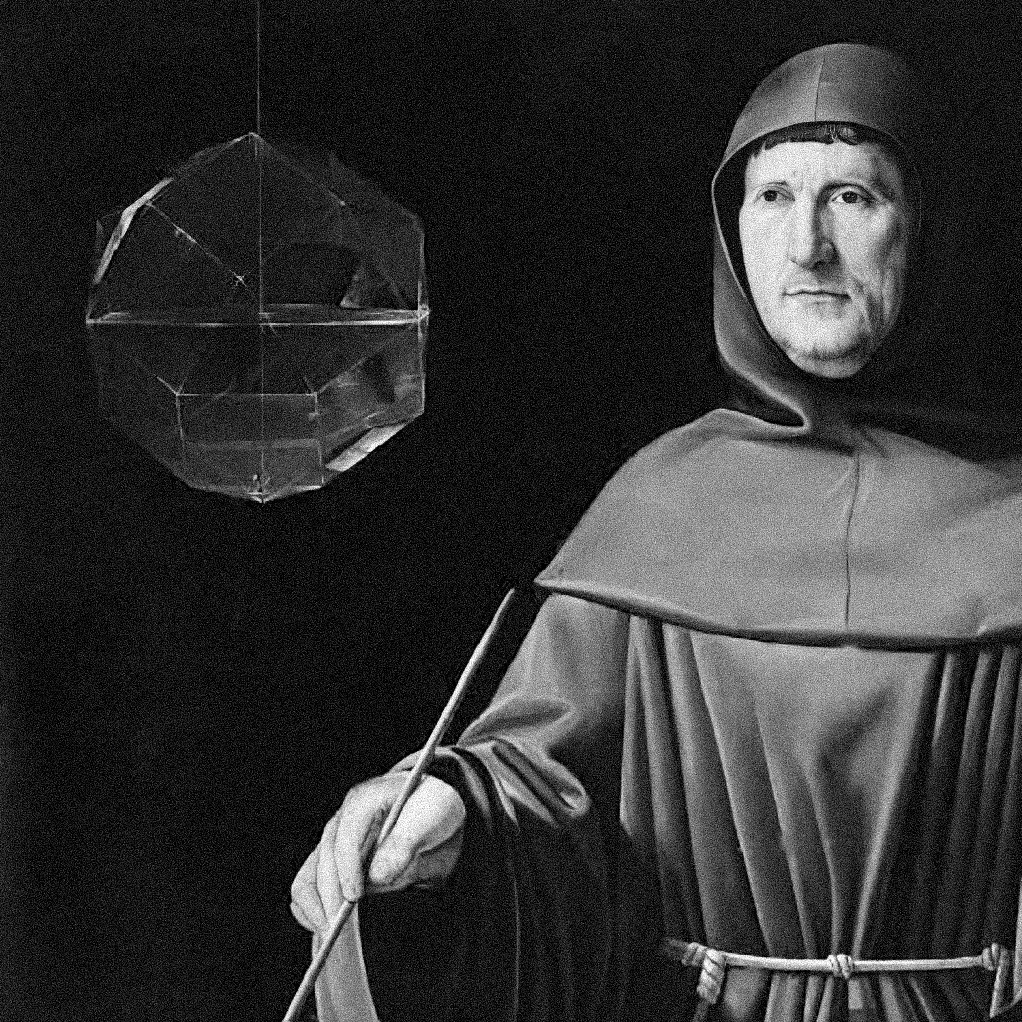
\includegraphics[width=\linewidth]{Images/ApendiceC/PACIOLI.jpeg}
\textbf{Luca Pacioli:} Nacido alrededor del 1446 en Borgo San Sepolcro, fue un matemático, franciscano y escritor italiano. Es considerado como el padre de la contabilidad moderna debido a su obra \textit{Summa de Arithmetica, Geometría, Proportioni et Proportionalità} en la que desarrolló el método de contabilidad de partida doble. Además de su trabajo en contabilidad, también hizo contribuciones significativas a la geometría y la teoría de la proporción en la que fue un hombre muy respetado, donde también trabajó como profesor y tutor en varias partes de Italia. Pacioli murió en 1517, pero su influencia en las matemáticas y la contabilidad ha sido duradera.
}
\begin{center}
    \begin{tikzpicture}
        \filldraw[black] (0,0) rectangle (2,2);
        \filldraw[black!70] (3,0) rectangle (9,2);
        
        \node at (0,1) [left] {$x$};
        \node at (1,0) [below] {$x$};
        
        \node at (6,0) [below] {$26$};
        \node at (3,1) [left] {$x$};
    \end{tikzpicture}
\end{center}
donde el área de las anteriores figuras suman 27.

Hagamos el siguiente arreglo:
\begin{center}
    \begin{tikzpicture}
        \filldraw[black] (0,0) rectangle (2,2);
        
        \filldraw[black!70] (2,0) rectangle (6.5,2);
        
        \filldraw[black!70] (0,0) rectangle (2,-4.5);

        %\filldraw[black!80] (2,0) rectangle (6.5,-4.5);
        
        \node[white] at (0,1) [right] {$x$};
        \node[white] at (1,0) [above] {$x$};
        
        \node[white] at (2,1) [right] {$x$};
        \node[white] at (4.25,0) [above] {$13$};
        
        \node[white] at (0,-2.25) [right] {$13$};
        \node[white] at (1,-4.5) [above] {$x$};
    \end{tikzpicture}
\end{center}
pero podemos completar el cuadrado añadiendo un cuadrado de $13 \times 13$, es decir
\begin{center}
    \begin{tikzpicture}
        \filldraw[black] (0,0) rectangle (2,2);
        
        \filldraw[black!70] (2,0) rectangle (6.5,2);
        
        \filldraw[black!70] (0,0) rectangle (2,-4.5);

        \filldraw[black!80] (2,0) rectangle (6.5,-4.5);
        
        \node[white] at (0,1) [right] {$x$};
        \node[white] at (1,0) [above] {$x$};
        
        \node[white] at (2,1) [right] {$x$};
        \node[white] at (4.25,0) [above] {$13$};
        
        \node[white] at (0,-2.25) [right] {$13$};
        \node[white] at (1,-4.5) [above] {$x$};
    \end{tikzpicture}
\end{center}
Ahora obtendríamos una nueva ecuación, la cual es
$$x^2+26x+169=196.$$

Sabiendo que la raíz cuadrada de $196$ es $14$, se tiene:
\marginElement{\justify
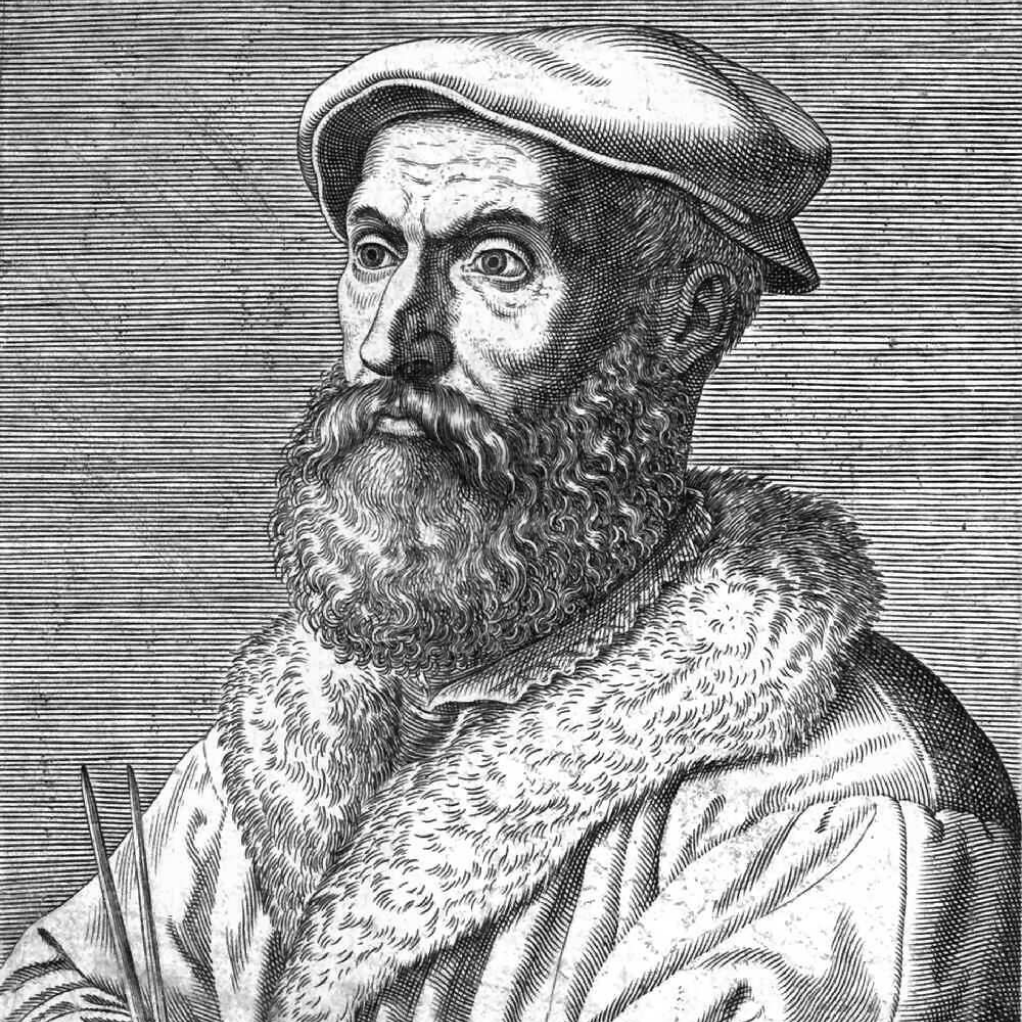
\includegraphics[width=\linewidth]{Images/ApendiceC/FONTANA.png}
\textbf{Niccolò Tartaglia:} Nacido en Brescia en 1499, es conocido por haber resuelto el problema de la cubatura, que consiste en determinar el volumen de una figura sólida. En 1543 publicó su obra \textit{Nova Scientia}, donde presentó sus descubrimientos en matemáticas y óptica, así como su método para resolver ecuaciones de tercer grado. Se le conocía por Tartaglia, ya que de niño había sufrido un corte en el rostro por parte de un soldado francés, lo que lo dejó tartamudo, de ahí se le conoce por \textit{tartaglia}, que es tartamudo en italiano. Tartaglia falleció en Venecia en 1557 y su legado ha sido reconocido por importantes matemáticos como Galileo Galilei y Johannes Kepler.
}
\begin{center}
    \begin{tikzpicture}
        \filldraw[black] (0,0) rectangle (2,2);
        
        \filldraw[black!70] (2,0) rectangle (6.5,2);
        
        \filldraw[black!70] (0,0) rectangle (2,-4.5);

        \filldraw[black!80] (2,0) rectangle (6.5,-4.5);
        
        \node[white] at (0,1) [right] {$x$};
        \node[white] at (1,0) [above] {$x$};
        
        \node[white] at (2,1) [right] {$x$};
        \node[white] at (4.25,0) [above] {$13$};
        
        \node[white] at (0,-2.25) [right] {$13$};
        \node[white] at (1,-4.5) [above] {$x$};

        \draw[snake=brace,thick] (6.6,2) -- (6.6,-4.5);
        
        \node at (6.7,-1.25) [right] {$14$};
    \end{tikzpicture}
\end{center}
Por lo que $x=1$. Lo anterior, es una forma visual de resolver una ecuación cuadrática, pero no es completa. Si $x=1$, podemos ver que es una solución de $x^2+26x=27$, pero también lo es $-27$. Por miles de años, los matemáticos ignoraban las soluciones negativas de sus ecuaciones porque  trataban con las cosas del mundo real (longitud, área y volumen). Para aquellos matemáticos, los números negativos no existían, se podía restar, pero no se podía tener una respuesta negativa ni coeficientes negativos. No existía una ecuación cuadrática como $ax^2+bx+c=0$, sino habían seis versiones diferentes para que los coeficientes siempre fueran positivos.

No fue hasta que Scipione Del Ferro, al rededor del año 1510, descubrió un método para resolver ecuaciones cúbicas reducidas, estas son una selección de ecuaciones cúbicas sin término elevado al cuadrado. Del Ferro no publicó sus resultados, ya que al mantener la solución en secreto, se aseguraba de mantener su empleo. Esto lo hizo durante casi dos décadas, y no fue hasta su lecho de muerte, en 1526, que se lo dejó entrever a su discípulo Antonio Maria del Fior. Luego de la muerte de Del Ferro, Fior desafío al gran matemático Niccolò Fontana Tartaglia, también italiano, a que resolviera un cierto número de ecuaciones de tercer grado. Fior no pudo resolver ni un solo problema, mientras que Tartaglia, antes del plazo fijado en este (40 días), encontró un método para resolver cualquier ecuación cúbica de la forma $x^3+px+q=0$. Antes del desafío, Tartaglia se entero que Fior se jactaba de haber resuelto la cúbica reducida, pero no lo creyó. Se corría el rumor de que un gran matemático le había revelado el secreto a Fior, lo que era más posible, así que sabiendo que una solución a la cúbica era posible y con su reputación en riesgo, se propuso resolver la cúbica reducida él mismo. Para hacerlo, exploró la idea de completar el cuadrado en tres dimensiones. Imaginemos que queremos resolver la ecuación
\begin{equation}
    x^3+9x=26 \label{ecuacioncardanoaresolver}
\end{equation}
entonces
\begin{multicols}{2}
    \begin{center}
        \begin{tikzpicture}[scale=0.8,
                    x  = {(0.5cm,0.5cm)},
                    y  = {(0.95cm,-0.25cm)},
                    z  = {(0cm,0.9cm)}]
            
            %%Cara izquierda%%
            \begin{scope}[canvas is yz plane at x=-1]
            
                \shade[left color=black!70,right color=black!80] (-1,-1) rectangle (1,1);
                \draw[black,decorate,decoration={brace,mirror,raise=4pt},thick,transform shape] (-1,-1) -- (1,-1);
                \draw[black,decorate,decoration={brace,raise=4pt},thick,transform shape] (-1,-1) -- (-1,1);
            \end{scope}
            
            \begin{scope}[canvas is xz plane at y=1]
            
                \shade[right color=black!60,left color=black!80] (-1,-1) rectangle (1,1);
                \draw[black,decorate,decoration={brace,mirror,raise=4pt},thick,transform shape] (-1,-1) -- (1,-1);
                \node[black] at (-5.9,3.2) [xscale=1] {$x$};
            \end{scope}
            
            \begin{scope}[canvas is yx plane at z=1]
            
                \shade[top color=black!90,bottom color=black!80] (-1,-1) rectangle (1,1);
                
                \node[black] at (3,-3.1) [xscale=1,transform shape,rotate=90] {\Large $x$};
                
                \node[black] at (1.6,-4.5) [xscale=1,transform shape] {\Large $x$};
                
                \node at (0,0) [xscale=1,transform shape,white] {$x^3$};
            \end{scope}
        \end{tikzpicture}
    \end{center}

\columnbreak

    \begin{flushleft}
        \begin{tikzpicture}[scale=0.8,
                    x  = {(0.5cm,0.5cm)},
                    y  = {(0.95cm,-0.25cm)},
                    z  = {(0cm,0.9cm)}]
            
            %%Segundo rectángulo%%
            \begin{scope}[canvas is yz plane at x=-1]
            
                \shade[left color=black!50,right color=black!70] (4,-1) rectangle (8,1);
            \end{scope}
            
            \begin{scope}[canvas is xz plane at y=5.368]
            
                \shade[right color=black!80,left color=black!70] (4,-4.509) rectangle (6,-2.509);
            \end{scope}
            
            \begin{scope}[canvas is yx plane at z=1]
            
                \shade[top color=black!90,bottom color=black!70] (4,-1) rectangle (8,1);
                
                \node at (6,0) [xscale=1,transform shape,white] {$9x$};
            \end{scope}
        \end{tikzpicture}
    \end{flushleft}
\end{multicols}
\noindent
donde la suma de los anteriores volúmenes sumen $26$.

Imaginemos extender tres lados del cubo $x^3$, una distancia $y$, es decir
\begin{center}
    \begin{tikzpicture}[scale=0.9,
                    x  = {(0.5cm,0.5cm)},
                    y  = {(0.95cm,-0.25cm)},
                    z  = {(0cm,0.9cm)}]

        \draw[dash pattern=on 3pt off 3pt] (-0.42,0.95) -- (-0.42,3) node [above] {$y$};
        %%Cara izquierda%%
        \begin{scope}[canvas is yz plane at x=-1]
            
            \shade[left color=black!70,right color=black!80] (-1,-1) rectangle (1,1);
        
        \end{scope}
            
        \begin{scope}[canvas is xz plane at y=1]

            \node[black] at (-5.6,3) [xscale=1] {$x$};
            
            \shade[right color=black!60,left color=black!80] (-1,-1) rectangle (1,1);

            \draw[dash pattern=on 3pt off 3pt] (-2.76,3) -- (-2.76,5) node [right] {$y$};
            
            \draw[dash pattern=on 3pt off 3pt] (-1.1,-1) -- (-2.8,-1) node [left] {$y$};
        \end{scope}
            
        \begin{scope}[canvas is yx plane at z=1]
            
            \shade[top color=black!90,bottom color=black!80] (-1,-1) rectangle (1,1);
                
            \node[black] at (3,-3.1) [xscale=1,transform shape,rotate=90] {\Large $x$};
                
            \node[black] at (1.6,-4.5) [xscale=1,transform shape] {\Large $x$};
                
            \node at (0,0) [xscale=1,transform shape,white] {$x^3$};
        \end{scope}
    \end{tikzpicture}
\end{center}
Por lo que se crea un nuevo cubo y más grande, cuyos lados ahora midan $z$, siendo $z=x+y$, es decir:
\begin{center}
    \begin{tikzpicture}[scale=1.1,
                    x  = {(0.5cm,0.5cm)},
                    y  = {(0.95cm,-0.25cm)},
                    z  = {(0cm,0.9cm)}]
        
        \begin{scope}[canvas is yz plane at x=-0.5]
        
            \shade[left color=black!50,right color=black!70] (-0.5,-0.5) rectangle (0.5,0.5);
        
        \end{scope}
        
        \begin{scope}[canvas is xz plane at y=0.5]
        
            \shade[right color=black!80,left color=black!70] (-0.5,-0.5) rectangle (0.5,0.5);
            
        \end{scope}
        
        \begin{scope}[canvas is yx plane at z=0.5]
        
            \shade[top color=black!90,bottom color=black!70] (-0.5,-0.5) rectangle (0.5,0.5);
            
        \end{scope}              
        
        %%Cara izquierda%%
        \begin{scope}[canvas is yz plane at x=-1]
        
            \shade[left color=black!20,right color=black!20,opacity=0.5] (-1,-1) rectangle (1,1);
            
            \draw[black,decorate,decoration={brace,mirror,raise=4pt},thick,transform shape] (-1,-1) -- (1,-1);
            \draw[black,decorate,decoration={brace,raise=4pt},thick,transform shape] (-1,-1) -- (-1,1);
            
        \end{scope}
        
        \begin{scope}[canvas is xz plane at y=1]
        
            \shade[right color=black!70,left color=black!20,opacity=0.5] (-1,-1) rectangle (1,1);
            \draw[black,decorate,decoration={brace,mirror,raise=4pt},thick,transform shape] (-1,-1) -- (1,-1);
            
            \node[black] at (-5.5,3.1) [xscale=1] {$z$};
            
        \end{scope}
        
        \begin{scope}[canvas is yx plane at z=1]
        
            \shade[top color=black!80,bottom color=black!20,opacity=0.5] (-1,-1) rectangle (1,1);
            
            \node[black] at (3,-3.1) [xscale=1,transform shape,rotate=90] {\footnotesize $z$};
            
            \node[black] at (1.6,-4.5) [xscale=1,transform shape] {\footnotesize $z$};
            
        \end{scope}
    \end{tikzpicture}
\end{center}
Podemos dividir el volumen adicional en siete formas:
\begin{center}
    \begin{tikzpicture}[scale=0.9,
                    x  = {(0.5cm,0.5cm)},
                    y  = {(0.95cm,-0.25cm)},
                    z  = {(0cm,0.9cm)}]
        %%%%CUBO CAFÉ%%%%
        %%Cara izquierda%%
        \begin{scope}[canvas is yz plane at x=-1]
            \shade[left color=black!50,right color=black!70] (-1,-4) rectangle (1,-2);
        \end{scope}
        
        %%Cara derecha%%
        \begin{scope}[canvas is xz plane at y=1]
            \shade[right color=black!80,left color=black!70] (-1,-4) rectangle (1,-2);
        \end{scope}
        
        %%Cara superior%%
        \begin{scope}[canvas is yx plane at z=-2]
            \shade[top color=black!90,bottom color=black!70] (-1,-1) rectangle (1,1);
        \end{scope}
        %%%%CUBO CAFÉ%%%%
        
        %%%%CUBO AZUL SUPERIOR%%%%
        %%Cara izquierda%%
        \begin{scope}[canvas is yz plane at x=-1]
            \shade[left color=black!50,right color=black!20] (-1,0) rectangle (1,1);
        \end{scope}
        
        %%Cara derecha%%
        \begin{scope}[canvas is xz plane at y=1]
            \shade[right color=black!70,left color=black!20] (-1,0) rectangle (1,1);
        \end{scope}
        
        %%Cara superior%%
        \begin{scope}[canvas is yx plane at z=1]
            \shade[top color=black!80,bottom color=black!20] (-1,-1) rectangle (1,1);
        \end{scope}
        %%%%CUBO AZUL SUPERIOR%%%%
        
        %%%%CUBO AZUL IZQUIERDA%%%%
        %%Cara izquierda%%
        \begin{scope}[canvas is yz plane at x=-3]
            \shade[left color=black!50,right color=black!20] (-1,-4) rectangle (1,-2);
            \draw[black,decorate,decoration={brace,mirror,raise=4pt},thick,transform shape] (-1,-4) -- (1,-4); 
            \draw[black,decorate,decoration={brace,raise=4pt},thick,transform shape] (-1,-4) -- (-1,-2);
        \end{scope}
        
        %%Cara derecha%%
        \begin{scope}[canvas is xz plane at y=1]
            \shade[right color=black!70,left color=black!20] (-3,-4) rectangle (-2,-2);
            \draw[black,decorate,decoration={brace,mirror,raise=4pt},thick,transform shape] (-3,-4) -- (-2,-4);
            \node[black] at (-7.6,0.1) [xscale=1] {$x$};
        \end{scope}
        
        %%Cara superior%%
        \begin{scope}[canvas is yx plane at z=-2]
            \shade[top color=black!80,bottom color=black!20] (-1,-3) rectangle (1,-2);
            \node[black] at (3,-5.6) [xscale=1,transform shape,rotate=90] {$y$};
            \node[black] at (1.6,-6.5) [xscale=1,transform shape] {$x$};
        \end{scope}
        %%%%CUBO AZUL IZQUIERDA%%%%
        
        %%%%CUBO AZUL DERECHA%%%%
        %%Cara izquierda%%
        \begin{scope}[canvas is yz plane at x=-1]
            \shade[left color=black!50,right color=black!20] (2,-4) rectangle (3,-2);
        \end{scope}
        
        %%Cara derecha%%
        \begin{scope}[canvas is xz plane at y=3]
            \shade[right color=black!70,left color=black!20] (-1,-4) rectangle (1,-2);
        \end{scope}
        
        %%Cara superior%%
        \begin{scope}[canvas is yx plane at z=-2]
            \shade[top color=black!80,bottom color=black!20] (2,-1) rectangle (3,1);
        \end{scope}
        %%%%CUBO AZUL DERECHA%%%%
        
        %%%%CUBO VERDE DERECHA%%%%
        %%Cara izquierda%%
        \begin{scope}[canvas is yz plane at x=-1]
            \shade[left color=black!50,right color=black!20] (2,0) rectangle (3,1);
        \end{scope}
        
        %%Cara derecha%%
        \begin{scope}[canvas is xz plane at y=3]
            \shade[right color=black!70,left color=black!20] (-1,0) rectangle (1,1);
        \end{scope}
        
        %%Cara superior%%
        \begin{scope}[canvas is yx plane at z=1]
            \shade[top color=black!80,bottom color=black!20] (2,-1) rectangle (3,1);
        \end{scope}
        %%%%CUBO VERDE DERECHA%%%%
        
        %%%%CUBO VERDE IZQUIERDA%%%%
        %%Cara izquierda%%
        \begin{scope}[canvas is yz plane at x=-3]
            \shade[left color=black!50,right color=black!20] (-1,0) rectangle (1,1);
        \end{scope}
        
        %%Cara derecha%%
        \begin{scope}[canvas is xz plane at y=1]
            \shade[right color=black!70,left color=black!20] (-3,0) rectangle (-2,1);
        \end{scope}
        
        %%Cara superior%%
        \begin{scope}[canvas is yx plane at z=1]
            \shade[top color=black!80,bottom color=black!20] (-1,-3) rectangle (1,-2);
        \end{scope}
        %%%%CUBO VERDE IZQUIERDA%%%%
        
        %%%%CUBO VERDE CENTRO%%%%
        %%Cara izquierda%%
        \begin{scope}[canvas is yz plane at x=-3]
            \shade[left color=black!50,right color=black!20] (2,-4) rectangle (3,-2);
            \draw[black,decorate,decoration={brace,mirror,raise=4pt},thick,transform shape] (2,-4) -- (3,-4); 
            \draw[black,decorate,decoration={brace,raise=4pt},thick,transform shape] (2,-4) -- (2,-2);
        \end{scope}
        
        %%Cara derecha%%
        \begin{scope}[canvas is xz plane at y=3]
            \shade[right color=black!70,left color=black!20] (-3,-4) rectangle (-2,-2);
            \draw[black,decorate,decoration={brace,mirror,raise=4pt},thick,transform shape] (-3,-4) -- (-2,-4);
            %\node[black] at (-5.8,-1.2) [xscale=1] {$x$};
        \end{scope}
        
        %%Cara superior%%
        \begin{scope}[canvas is yx plane at z=-2]
            \shade[top color=black!80,bottom color=black!20] (2,-3) rectangle (3,-2);
            \node[black] at (5,-5.6) [xscale=1,transform shape,rotate=90] {$y$};
            \node[black] at (4.1,-6.5) [xscale=1,transform shape] {$y$};
        \end{scope}
        %%%%CUBO VERDE CENTRO%%%%
        
        %%%%CUBO NARANJA%%%%
        %%Cara izquierda%%
        \begin{scope}[canvas is yz plane at x=-3]
            \shade[left color=black!40,right color=black!10] (2,0) rectangle (3,1);
            \draw[gray,decorate,decoration={brace,mirror,raise=4pt},thick,transform shape] (2,0) -- (3,0); 
            \draw[gray,decorate,decoration={brace,raise=4pt},thick,transform shape] (2,0) -- (2,1);
        \end{scope}
        
        %%Cara derecha%%
        \begin{scope}[canvas is xz plane at y=3]
            \shade[right color=black!70,left color=black!20] (-3,0) rectangle (-2,1);
            \draw[gray,decorate,decoration={brace,mirror,raise=4pt},thick,transform shape] (-3,-0) -- (-2,0);
            \node[gray] at (-5.8,2.3) [xscale=1] {$y$};
        \end{scope}
        
        %%Cara superior%%
        \begin{scope}[canvas is yx plane at z=1]
            \shade[top color=black!80,bottom color=black!20] (2,-3) rectangle (3,-2);
            %\node[gray] at (4.3,-4.2) [xscale=1,transform shape,rotate=90] {$y$};
            \node[gray] at (3.4,-5.1) [xscale=1,transform shape] {$y$};
        \end{scope}
        %%%%CUBO NARANJA%%%%
    \end{tikzpicture}
\end{center}

Tartaglia reordenó los anteriores prismas en un bloque nuevo. Este tiene un lado que mide $3y$, el otro mide $x+y$ (que es $z$), y de altura $x$, es decir:
\begin{center}
    \begin{tikzpicture}[
                    x  = {(0.5cm,0.5cm)},
                    y  = {(0.95cm,-0.25cm)},
                    z  = {(0cm,0.9cm)}]
        %%%%CUBOS AZULES SUPERIOR%%%%
        %%Cara izquierda%%
        \begin{scope}[canvas is yz plane at x=-1]
            \shade[left color=black!50,right color=black!20] (-1,-1) rectangle (1,1);
            \shade[left color=black!50,right color=black!20] (1,-1) rectangle (2,1);
            \draw[black,decorate,decoration={brace,raise=4pt},thick,transform shape] (-1,-1) -- (-1,1);
        \end{scope}
        
        \begin{scope}[canvas is yz plane at x=-2]
            \draw[black,decorate,decoration={brace,mirror,raise=4pt},thick,transform shape] (-1,-1) -- (2,-1); 
        \end{scope}
        
        %%Cara derecha%%
        \begin{scope}[canvas is xz plane at y=2]
            \shade[right color=black!70,left color=black!20] (-1,-1) rectangle (0,1);
            \shade[right color=black!70,left color=black!20] (0,-1) rectangle (1,1);
            \shade[right color=black!70,left color=black!20] (1,-1) rectangle (2,1);
            \draw[black,decorate,decoration={brace,mirror,raise=4pt},thick,transform shape] (-1,-1) -- (2,-1);
            \node[black] at (-7.6,4.5) [xscale=1] {$x$};
        \end{scope}
        
        %%Cara superior%%
        \begin{scope}[canvas is yx plane at z=1]
            \shade[top color=black!80,bottom color=black!20] (-1,-1) rectangle (1,0);
            \shade[top color=black!80,bottom color=black!20] (-1,0) rectangle (1,1);
            \shade[top color=black!80,bottom color=black!20] (-1,1) rectangle (1,2);
            
            \shade[top color=black!80,bottom color=black!20] (1,-1) rectangle (2,0);
            \shade[top color=black!80,bottom color=black!20] (1,0) rectangle (2,1);
            \shade[top color=black!80,bottom color=black!20] (1,1) rectangle (2,2);
            
            \node[black] at (4,-2.6) [xscale=1,transform shape,rotate=90] {$3y$};
            
            \node[black] at (1.6,-4.5) [xscale=1,transform shape] {$x$};
            \node[black] at (3,-4.5) [xscale=1,transform shape] {$y$};
            \node[black] at (2.1,-5.5) [xscale=1,transform shape] {$z$};
        \end{scope}
        %%%%CUBO AZUL SUPERIOR%%%%
    \end{tikzpicture}
\end{center}
El volumen de dicha figura está dado por
$$V=(3y)(z)(x)$$
y este mismo puede representar el término $9x$ si su base es igual a 9. En consecuencia
\begin{equation}
    3yz=9 \label{KKKKK}
\end{equation}
sumando $y^3$ a \eqref{ecuacioncardanoaresolver}, obtenemos
$$x^3+9x+y^3=26+y^3$$
se sigue que
\begin{equation}
    z^3=26+y^3. \label{YAYAYAYAYA}
\end{equation}
Al resolver \eqref{KKKKK}, obtenemos que $\displaystyle z=\frac{3}{y}$. Sustituyendo en \eqref{YAYAYAYAYA}, se sigue que
$$y^3+26=\frac{27}{y^3}$$
es decir,
$$y^6+26y^3=27.$$

A primera vista podría parecer que empeoramos el problema que queríamos resolver, ya que la variable ahora está elevado a la $6$ en lugar de $3$. Sin embargo, si pensamos a $y^3$ como una nueva variable, digamos $r=y^3$, la ecuación acaba siendo una ecuación cuadrática
$$r^2+26r=27$$
la misma que resolvimos anteriormente \eqref{ULTIMOYAYAYA}. En consecuencia $y^3=1$, por lo que $y=1$. Sabemos que $\displaystyle z = \frac{3}{y}$, pero $y=1$, por lo que $z=3$. Además, sabemos que $x+y=z$, entonces $x=2$. Lo que es la solución a la ecuación \eqref{ecuacioncardanoaresolver}.

Así como Del Ferro, Tartaglia no publicó su método; pero un profesor de física y matemática de Milán, Cardano, lo convenció de que se lo comunicara, bajo la promesa de mantenerlo en secreto. Cardano violó su promesa y publicó el resultado de Tartaglia en su trabajo \textit{Ars Magna} en 1545. Desde entonces, las fórmulas para resolver una ecuación de tercer grado se conocen como fórmulas de Cardano. Poco después de la resolución de la ecuación cúbica, el también matemático italiano, alumno de Cardano, Ferrari resolvió la ecuación general de cuarto grado.\marginElement{\justify
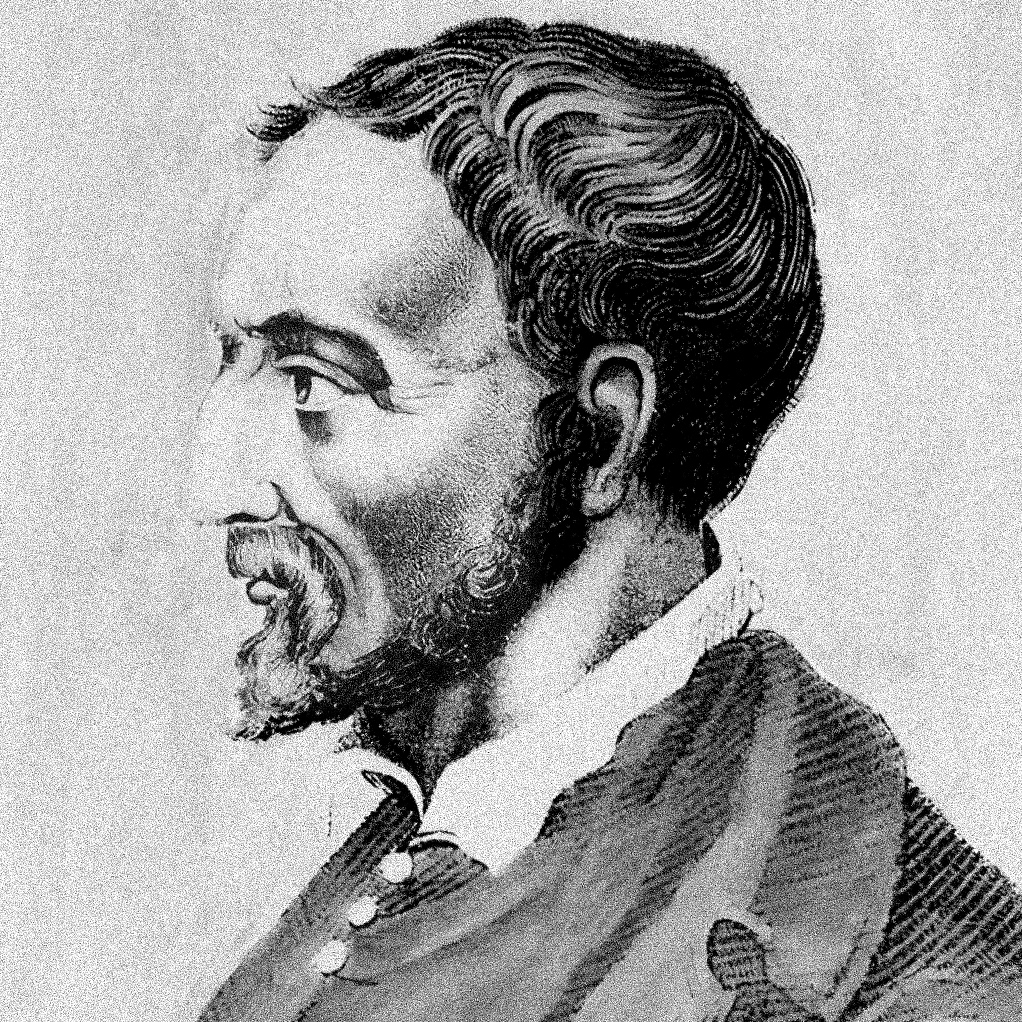
\includegraphics[width=\linewidth]{Images/ApendiceC/CARDANO.jpeg}
\textbf{Girolamo Cardano:} Nacido en Pavía en 1501, destacó por sus aportes significativos en la matemática; en áreas como la teoría de ecuaciones, la geometría y la probabilidad donde introdujó el número negativo en la teoría matemática y la resolución de ecuaciones de tercer grado. Además de sus aportes en matemáticas, Cardano comenzó a estudiar medicina a los 23 años, obteniendo su doctorado en 1525. Fue uno de los primeros médicos en practicar la autopsia y realizar estudios sobre la anatomía y fisiología humana. También, fue un astrólogo reconocido en su época y escribió varias obras sobre el tema. Falleció en Roma en 1576.
}

Los procesos que expondremos en esta apéndice, para obtener las fórmulas para resolver las ecuaciones de tercer y cuarto grados, se sustentan en los trabajos de los matemáticos italianos antes mencionados, y se basan en transformaciones especiales y complicadas de la ecuación respectiva, que bien pueden parecer artificiales y accidentales, pero que ocurrieron en la intensa búsqueda de métodos para resolver dichas ecuaciones.

\begin{observation}
    De la ecuación de primer grado, es decir
    $$ax+b=0$$
    solo diremos que su única solución es $\displaystyle x=-\frac{b}{a}$.
\end{observation}

\section{La definición del discriminante}

\begin{definition}\label{definicion:B.1.1}
    Consideremos la ecuación de grado $n \geq 2$ y coeficientes complejos dada por
    $$a_nx^n+\cdots +a_1x+a_0=0$$
    y sean $x_1, x_2, \dots, x_n$ sus raíces (no necesariamente distintas). Definimos el discriminante de esta ecuación como
    $$D=a_n^{2n-2}\prod_{1 \leq i < j \leq n}(x_i-x_j)^2.$$
\end{definition}

\begin{observation}
    En lugar de la ecuación
    $$a_nx^n+\cdots +a_1x+a_0=0$$
    de la definición anterior, podemos hablar del polinomio
    $$f(x)=a_nx^n+\cdots +a_1x+a_0.$$
    En este caso, se dice que
    $$D=a_n^{2n-2}\prod _{1 \leq i < j \leq n}(x_i-x_j)^2$$
    es el discriminante del polinomio $f(x)$.
\end{observation}

\section{Ecuación de segundo grado}

Consideremos la ecuación general de segundo grado, donde $a, b, c \in \CC$ y $a \neq 0$, con la incógnita $x$:
\begin{equation}
    ax^2+bx+c=0. \label{ecuaciongrado2}
\end{equation}
Si $r$ es raíz de \eqref{ecuaciongrado2}, entonces
\begin{equation}
    ar^2+br+c=0. \label{ecuaciongrado2.1}
\end{equation}
Multiplicando ambos miembros de \eqref{ecuaciongrado2.1} por $4a$, obtenemos
\begin{equation*}
    4a^2r^2+4abr+4ac=0. \label{ecuaciongrado2.2}
\end{equation*}
Sumando $b^2-4ac$ en ambos miembro de \eqref{ecuaciongrado2.2}, obtenemos
$$4a^2r^2+4abr+b^2=b^2-4ac $$
es decir,
$$(2ar+b)^2 = b^2-4ac$$
por tanto
$$2ar+b = \pm \sqrt{b^2-4ac}$$
y por ende,
$$r = \frac{-b \pm \sqrt{b^2-4ac}}{2a}$$\newpage
Nótese que $b^2-4ac$ es un número complejo, por lo que tiene dos raíces complejas $z$ y $w$, donde $w=-z$. Así que $\sqrt{b^2-4ac}$ representa a cualquiera, pero solo a una, de $z$ y $w$.

En resumen, las dos raíces (no necesariamente distintas) de la ecuación $ax^2+bx+c=0$ vienen dadas por la fórmula
$$x=\frac{-b \pm \sqrt{b^2-4ac}}{2a}.$$

\section{El discriminante de la ecuación de segundo grado}

Por la sección anterior, sabemos que las raíces de $ax^2+bx+c=0$ son
$$x_1=\frac{-b + \sqrt{b^2-4ac}}{2a} \hspace{0.5cm} \text{y} \hspace{0.5cm} x_2=\frac{-b - \sqrt{b^2-4ac}}{2a}.$$
Por lo que el discriminante de dicha ecuación es
$$D=a^2(x_1-x_2)^2,$$
es decir:
$$D=b^2-4ac.$$

\begin{observation}
    Si la ecuación de segundo grado $ax^2+bx+c=0$ es de coeficientes reales, entonces:
    \begin{enumerate}[label=\roman*.]
        \item Tiene dos raíces reales si y solo si $D>0$.
        \item Tiene una raíz real doble si y solo si $D=0$.
        \item Tienen dos raíces imaginarias diferentes si y solo si $D<0$.
    \end{enumerate}
\end{observation}

\section{La ecuación de tercer grado} \label{sec:B4}

Consideremos la ecuación general de tercer grado
\begin{equation}
    Ax^3+Bx^2+Cx+D=0 \label{ecuaciongrado3}
\end{equation}
con $A,  B,  C,  D \in \CC$ y $A \neq 0$ y con la incógnita $x$. Como $A \neq 0$, y puesto que la ecuación
$$\frac{1}{A} \left( Ax^3+Bx^2+Cx+D \right) =0$$
tiene las mismas raíces que la ecuación \eqref{ecuaciongrado3}, entonces no se pierde generalidad si en lugar de esta, escribimos
\begin{equation}
    x^3+bx^2+cx+d=0, \text{ con }  b,  c,  d \in \CC \label{ecuaciongrado3.1}
\end{equation}

Sustituyendo $\displaystyle x=y-\frac{b}{3}$ en \eqref{ecuaciongrado3.1}, se tiene que
$$\left( y-\frac{b}{3} \right)^3+b \left( y-\frac{b}{3} \right)^2+c \left( y-\frac{b}{3} \right) +d=0,$$
por tanto
$$y^3+\left( c-\frac{b^2}{3} \right) y + \left( d-\frac{bc}{3}+\frac{2b^3}{27} \right) =0.$$\newpage

En consecuencia, resolver la ecuación \eqref{ecuaciongrado3.1} se reduce a resolver la ecuación
$$y^3+py+q=0$$
donde
$$p=c-\frac{b^2}{3} \hspace{0.5cm} \text{y} \hspace{0.5cm} q=d-\frac{bc}{3}+\frac{2b^3}{27}.$$

Si $y_1$, $y_2$, $y_3$ son raíces de $y^3+py+q=0$, entonces:
$$x_1=y_1-\frac{b}{3} \hspace{1cm} x_2=y_2-\frac{b}{3} \hspace{1cm} x_3=y_3-\frac{b}{3}$$
son las raíces de \eqref{ecuaciongrado3.1}.

Resolveremos ahora la ecuación
\begin{equation}
    y^3+py+q=0. \label{ecuaciongrado3.2}
\end{equation}
Escribiendo $y=u+v$ en \eqref{ecuaciongrado3.2}, tenemos que
$$(u+v)^3+p(u+v)+q=0.$$
Desarrollando la expresión anterior, obtenemos
\begin{equation}
    u^3+v^3+q+(3uv+p)(u+v)=0. \label{ecuaciongrado3.3}
\end{equation}

Cualquiera que sea el valor numérico de la suma de $u$ y $v$, siempre podemos determinar a $u$ y $v$ imponiéndoles la condición adicional que su producto $uv$ sea un número prefijado. En efecto: supongamos que $u+v=r$ e impongamos la condición adicional $uv=s$, entonces $v=r-u$ y $uv=s$, por tanto $v=r-u$ y $u(r-u)=s$, por tanto $v=r-u$ y $u^2-r u+s=0$. En consecuencia $v=r-u$, y $u$ puede calcularse por la fórmula para resolver una ecuación de segundo grado. Esto demuestra lo que se afirmó.

Enseguida determinaremos a $u$ y $v$, sabiendo que la suma $u+v$ es raíz de la ecuación $y^3+p y+q=0$, e imponiendo la condición adicional
\begin{equation}
    uv=-\frac{p}{3}. \label{ecuaciongrado3.4}
\end{equation}
Sustituyendo \eqref{ecuaciongrado3.4} en \eqref{ecuaciongrado3.3}, tenemos que
\begin{equation}
    u^3+v^3+q=0. \label{ecuaciongrado3.5}
\end{equation}
De \eqref{ecuaciongrado3.4} y \eqref{ecuaciongrado3.5}, se sigue que
\begin{equation}
    u^3v^3=-\frac{p^3}{27} \label{ecuaciongrado3.6}
\end{equation}
y
\begin{equation}
    u^3+v^3=-q. \label{ecuaciongrado3.7}
\end{equation}

Puesto que
$$(z-u^3)(z-v^3)=z^2-(u^3+v^3)z+u^3v^3$$
entonces por \eqref{ecuaciongrado3.6} y \eqref{ecuaciongrado3.7}, $u^3$ y $v^3$ son las dos soluciones de la ecuación de segundo grado
\begin{equation}
    z^2+qz-\frac{p^3}{27}=0. \label{ecuaciongrado3.8}
\end{equation}

Por otro lado, las soluciones de la ecuación \eqref{ecuaciongrado3.8}, vienen dadas por
$$z_1=-\frac{q}{2}+\sqrt{\frac{q^2}{4}+\frac{p^3}{27}} \hspace{1cm} \text{y} \hspace{1cm} z_2=-\frac{q}{2}-\sqrt{\frac{q^2}{4}+\frac{p^3}{27}}.$$\newpage

Por tanto, podemos escribir
\begin{equation}
    u^3=z_1 \hspace{1cm} \text{y} \hspace{1cm} v^3=z_2. \label{ecuaciongrado3.9}
\end{equation}

Nótese que las anteriores ecuaciones son del tipo $x^n=z$, por lo que se pueden resolver mediante el método expuesto en el \hyperref[FUNDAMENTAL]{Apéndice C}. Cada una de dichas ecuaciones tiene tres raíces, digamos $u_1$, $u_2$, $u_3$, para $u^3=z_1$; y $v_1$, $v_2$, $v_3$, para $v^3=z_2$.

Resolviendo la ecuación $x^3=1$, tenemos que sus raíces son:
$$w^0=1 \hspace{1cm} w=\frac{-1+\sqrt{3}i}{2} \hspace{1cm} w^2=\frac{-1-\sqrt{3}i}{2}$$

Es fácil comprobar que las raíces de
$$u^3=z_1$$
son:
$$u_1 \hspace{1cm} u_2=wu_1 \hspace{1cm} u_3=w^2u_1;$$
y las raíces de
$$v^3=z_2$$
son:
$$v_1 \hspace{1cm} v_2=wv_1 \hspace{1cm} v_3=w^2v_1.$$

No perdamos de vista que estamos determinando valores de $u$ y $v$, de modo que la suma $u+v$ sea raíz de $y^3+py+q=0$, y que además $u$ y $v$ satisfagan la condición adicional $\displaystyle uv=-\frac{p}{3}$. Hemos determinado tres posibles valores $u_1,  u_2$ y $u_3$ para $u$; y tres posibles valores $v_1,  v_2$ y $v_3$ para $v$.

Pero observemos que
$$\left(u_i v_j\right)^3=-\frac{p^3}{27}$$
no implica que
$$u_i v_j=-\frac{p}{3},$$
para cada $i,  j=1,  2,  3$. Si elegimos $u_1$ y $v_1$ de modo que $\displaystyle u_1v_1=-\frac{p}{3}$, y a los que denotaremos por
\begin{equation}
    u_1=\sqrt[3]{\frac{-q}{2}+\sqrt{\frac{q^2}{4}+\frac{p^3}{27}}} \label{APPCOSIPA1}
\end{equation}
y
\begin{equation}
    v_1=\sqrt[3]{\frac{-q}{2}-\sqrt{\frac{q^2}{4}+\frac{p^3}{27}}}. \label{APPCOSIPA2}
\end{equation}

Entonces las raíces de
$$y^3+py+q=0$$
son
\begin{equation}
    y_1=u_1+v_1 \hspace{1cm} y_2=wu_1+w^2v_1 \hspace{1cm} y_3=w^2u_1+wv_1. \label{APPCOSIPA3}
\end{equation}
Las expresiones anteriores son conocidas como \textit{fórmulas de Cardano}, para calcular las raíces de la ecuación $y^3+py+q=0$.

\newpage
\section{El discriminante de la ecuación de tercer grado}

De acuerdo a las fórmulas de Cardano, y a la definición \ref{definicion:B.1.1}, el discriminante de la ecuación $y^3+py+q=0$ es
$$D=(y_1-y_2)^2(y_1-y_3)^2(y_2-y_3)^2.$$

Recordemos que
$$w=-\frac{1}{2}+\frac{1}{2}\sqrt{3}i$$
es raíz de la ecuación $x^3-1=0$, por tanto
$$w^3=1 \hspace{0.5cm} \text{y} \hspace{0.5cm} w^2+w+1=0$$
entonces
\begin{align*}
    y_1-y_2 &=(u_1+v_1)-\left(wu_1+w^2v_1\right) \\
    &=(1-w)u_1-w^2v_1+w^3v_1 \\
    &=(1-w)u_1+(1-w)\left(-w^2v_1\right) \\
    &=(1-w)\left(u_1-w^2v_1\right), \\
    & \\
    y_1-y_3 &=(u_1+v_1)-\left( w^2u_1+wv_1 \right) \\
    &=\left( 1-w^2 \right) u_1-wv_1+w^3v_1 \\
    &=\left( 1-w^2 \right) u_1+\left( 1-w^2 \right) (-wv_1) \\
    &=\left( 1-w^2 \right) (u_1-wv_1), \\
    & \\
    y_2-y_3 &=\left( wu_1+w^2v_1 \right) - \left( w^2u_1+wv_1 \right) \\
    &=\left( w-w^2 \right) u_1-wv_1+w^2v_1 \\
    &=\left( w-w^2 \right) u_1+\left( w-w^2 \right) (-v_1) \\
    &=\left( w-w^2 \right) (u_1-v_1).
\end{align*}

Además
\begin{align*}
    (1-w)\left( 1-w^2 \right) &= \left( \frac{3}{2}-\frac{\sqrt{3}}{2} i \right) \left( \frac{3}{2}+\frac{\sqrt{3}}{2} i \right) \\
    &=3
\end{align*}
y
$$w-w^2=\sqrt{3}i.$$
Puesto que
$$(x-1)(x-w)\left( x-w^2 \right) =x^3-1,$$
entonces
$$\left( \frac{u_1}{v_1} -1 \right) \left( \frac{u_1}{v_1} -w \right) \left( \frac{u_1}{v_1}-w^2 \right) = \left( \frac{u_1}{v_1} \right)^3 -1$$
por tanto
\begin{equation}
    (u_1-v_1)(u_1-wv_1)\left( u_1-w^2v_1 \right) = u^3_1-v^3_1 \label{onono}
\end{equation}
Por \eqref{ecuaciongrado3.9} de la sección \ref{sec:B4}, de \eqref{onono} se sigue que
$$(u_1-v_1)(u_1-wv_1)\left( u_1-w^2v_1 \right) = 2 \sqrt{\frac{q^2}{4}+\frac{p^3}{27}}.$$
En consecuencia,
\begin{align*}
    D &=\left[ (y_1-y_2)(y_1-y_3)(y_2-y_3) \right]^2 \\
    &=\left[ (1-w)\left( u_1-w^2v_1 \right) \left( 1-w^2 \right) (u_1-wv_1) \left( w-w^2 \right) (u_1-v_1) \right]^2 \\
    &=\left[ (1-w) \left( 1-w^2 \right) \left( w-w^2 \right) (u_1-v_1) (u_1-wv_1) \left( u_1-w^2v_1 \right) \right]^2 \\
    &=\left[ 3 \left( \sqrt{3}i \right) \left( 2 \sqrt{\frac{q^2}{4}+\frac{p^3}{27}} \right) \right]^2 \\
    &= -108 \left( \frac{q^2}{4} + \frac{p^3}{27} \right) \\
    &=-27q^2-4p^3
\end{align*}

En resumen, el discriminante de la ecuación
\begin{equation}
    y^3+py+q=0 \label{TOCOF}
\end{equation}
es
$$D=-4p^3-27q^2.$$
Si $y_1$, $y_2$, $y_3$ son las raíces de \eqref{TOCOF}, donde
$$p=c-\frac{b^2}{3}$$
y
$$q=d-\frac{bc}{3}+\frac{2b^3}{27}$$
se sabe que
$$x_1 = y_1-\frac{b}{3} \hspace{1cm} x_2 = y_2-\frac{b}{3} \hspace{1cm} x_3 = y_3-\frac{b}{3}$$
son las raíces de
$$x^3+bx^2+cx+d=0.$$
Por tanto
$$x_1-x_2=y_1-y_2 \hspace{1cm} x_1-x_3=y_1-y_3 \hspace{1cm} x_2-x_3=y_2-y_3.$$

En consecuencia, el discriminante de
$$x^3+bx^2+cx+d=0$$
es
$$\Delta =-4p^3-27q^2,$$
es decir,
\begin{align*}
    \Delta & = -4 \left( c - \frac{b^2}{3} \right)^3 - 27 \left( d - \frac{bc}{3} + \frac{2b^3}{27} \right)^2 \\
    & =18bcd-4b^3d+b^2c^2-4c^3-27d^2.
\end{align*}

\begin{observation}
    Consideremos el escenario en el cual la ecuación cúbica
    $$x^3+bx^2+cx+d=0$$
    posee coeficientes reales (y por consiguiente, también su ecuación asociada $y^3 + py + q=0$ tiene coeficientes reales). Dado que esta ecuación es de grado impar, garantiza la existencia de al menos una raíz real. Por lo tanto, se presentan las siguientes tres posibilidades en relación con sus raíces:\newpage
    \begin{enumerate}[label=\roman*.]
        \item Tiene tres raíces reales diferentes.
        \item Tiene tres raíces reales y por lo menos dos de ellas iguales.
        \item Tiene una raíz real y dos raíces complejas conjugadas.
    \end{enumerate}
    En el primer caso, claramente, el discriminante $\Delta$ es positivo. En el segundo caso, el discriminante $\Delta$ es cero. En el tercer caso, el discriminante $\Delta$ es negativo, pues si $x_1=\alpha + \beta i$ y $x_2=\alpha - \beta i$ son las dos raíces complejas conjugadas, entonces
    \begin{align*}
        \Delta &=(x_1-x_2)^2 (x_1-x_3)^2 (x_2-x_3)^2 \\ 
        &= [2 \beta i]^2 [(\alpha - x_3)+\beta i]^2[(\alpha -x_3)-\beta i]^2 \\ 
        &=-4 \beta^2 \left[ (\alpha - x_3)^2+\beta^2 \right] <0
    \end{align*}
    Debido a las tres posibilidades anteriores, si una ecuación cúbica es de coeficientes reales, entonces:
    \begin{enumerate}[label=\roman*.]
        \item Si $\Delta >0$, entonces tiene tres raíces reales diferentes.
        \item Si $\Delta =0$, entonces tiene tres raíces reales y por lo menos dos de ellas son iguales.
        \item Si $\Delta <0$, entonces tiene una raíz real y dos raíces complejas conjugadas.
    \end{enumerate}
\end{observation}

\begin{example}
    Resuelva la ecuación
    $$y^3+3y^2-3y-14=0.$$
    \solucion Usando la sustitución $y=x-1$ reducimos esta ecuación a la forma
    $$x^3-6x-9=0.$$
    Notemos que $p=-6$ y $q=-9$, por lo cual
    $$\frac{q^2}{4}+\frac{p^3}{27}=\frac{49}{4}>0.$$
    Entonces, la ecuación
    $$x^3-6x-9=0$$
    tiene una raíz real y dos raíces complejas conjugadas. Según \eqref{APPCOSIPA1} y \eqref{APPCOSIPA2},
    $$u_1=\sqrt[3]{\frac{9}{2}+\frac{7}{2}}=\sqrt[3]{8} \quad \text{ y } \quad v_1=\sqrt[3]{\frac{9}{2}-\frac{7}{2}}=\sqrt[3]{1}.$$
    Por consiguiente, $u_1=2$ y $v_1=1$, es decir, $x_1=3$. Las otras dos raíces se hallan por las fórmulas \eqref{APPCOSIPA3}:
    $$x_2=-\frac{3}{2}+\frac{\sqrt{3}}{2}i \quad \text{ y } \quad x_3=-\frac{3}{2}-\frac{\sqrt{3}}{2}i.$$
    De aquí se deduce que las raíces de la ecuación dada son:
    $$y_1=2, \quad y_2=-\frac{5}{2}+\frac{\sqrt{3}}{2}i, \quad y_3=-\frac{5}{2}-\frac{\sqrt{3}}{2}i.$$
\end{example}

\begin{example}
    Resuelva la ecuación
    $$x^3-12x+16=0.$$
    \solucion Notemos que $p=-12$ y $q=16$, por lo tanto
    $$\frac{q^2}{4}+\frac{p^3}{27}=0.$$
    De esta ecuación, obtenemos $u_1=\sqrt[3]{-8}$, lo que implica que $u_1=-2$. En consecuencia, las raíces son $x_1=-4$ y $x_2=2=x_3$.
\end{example}

\newpage
\section{La ecuación de cuarto grado}

Consideremos la ecuación general de cuarto grado,
\begin{equation}
    Ax^4+Bx^3+Cx^2+Dx+E=0, \label{ecuacioncuarto7.1}
\end{equation}
donde $A,  B,  C,  D,  E \in \CC$ y $A \neq 0$, con la incógnita $x$.

Como $A \neq 0$, y puesto que la ecuación
$$\frac{1}{A} \left( Ax^4+Bx^3+Cx^2+Dx+E \right) =0$$
tiene las mismas raíces que la ecuación \eqref{ecuacioncuarto7.1}, entonces no se pierde generalidad si en lugar de esta, escribimos
\begin{equation}
    x^4+ax^3+bx^2+cx+d=0 \label{ecuacioncuarto7.2}
\end{equation}

Si la ecuación \eqref{ecuacioncuarto7.2} la escribimos en la forma
$$x^4+ax^3=-bx^2-cx-d$$
y sumamos $\displaystyle \frac{a^2}{4}x^2$ a ambos miembros de la ecuación, entonces
$$x^4+ax^3+\frac{a^2}{4}x^2=\frac{a^2}{4}x^2-bx^2-cx-d,$$
donde se sigue que
\begin{equation}
    \left( x^2+\frac{a}{2}x \right)^2 = \left( \frac{a^2}{4}-b \right) x^2-cx-d. \label{ecuacioncuarto7.3}
\end{equation}

Si el miembro derecho de la ecuación \eqref{ecuacioncuarto7.3} fuera un cuadrado perfecto, es decir, si fuera de la forma $(ex+f)^2$, entonces resolver dicha expresión y resolver \eqref{ecuacioncuarto7.2} sería inmediato. Pero en general dicho miembro derecho no es un cuadrado perfecto.

Sumando
$$\left( x^2+\frac{a}{2}x \right) y + \frac{y^2}{4}$$
a ambos miembros de \eqref{ecuacioncuarto7.3}, tenemos que
$$\left( x^2+\frac{a}{2}x \right)^2 + \left( x^2+\frac{a}{2}x \right) y + \frac{y^2}{4} = \left( \frac{a^2}{4}-b \right) x^2-cx-d + \left( x^2+\frac{a}{2}x \right) y + \frac{y^2}{4},$$
por tanto
\begin{equation}
    \left( x^2+\frac{a}{2}x+\frac{y}{2} \right)^2 = \left( \frac{a^2}{4}-b+y \right) x^2 + \left( -c+\frac{1}{2} ay \right) x+ \left( -d + \frac{1}{4} y^2 \right). \label{ecuacioncuarto7.4}
\end{equation}

Vamos a determinar $y$ de modo que el miembro derecho de la expresión \eqref{ecuacioncuarto7.4} sea un cuadrado perfecto. Para esto observemos que
$$Ax^2+Bx+C=(ex+f)^2,$$
si y solo si
$$B^2-4AC=0.$$
En efecto
\begin{align*}
    Ax^2+Bx+C=(ex+f)^2 & \Longrightarrow Ax^2+Bx+C=e^2x^2+2efx+f^2 \\ 
    & \Longrightarrow A=e^2, \; B=2ef, \; C=f^2 \\ 
    & \Longrightarrow B^2-4AC=0.
\end{align*}
Recíprocamente, si $B^2-4AC=0$, entonces
\begin{align*}
    Ax^2+Bx+C &=A \left( x^2+\frac{B}{A}x+\frac{C}{A} \right) \\
    &=A \left( x+\frac{B}{2A}-\frac{\sqrt{B^2-4AC}}{2A} \right) \left( x+\frac{B}{2A}+\frac{\sqrt{B^2-4AC}}{2A} \right) \\
    &=A \left( x+\frac{B}{2A} \right)^2 \\
    &=\left( \sqrt{A}x+\frac{B}{2\sqrt{A}} \right)^2 \\
    &=(ex+f)^2
\end{align*}
con $e=\sqrt{A}$ y $\displaystyle f=\frac{B}{2\sqrt{A}}$. En consecuencia, el miembro derecho de \eqref{ecuacioncuarto7.4} será un cuadrado perfecto, es decir,
$$\left( \frac{a^2}{4}-b+y \right) x^2+\left( -c+\frac{1}{2}ay \right) x + \left( -d+\frac{1}{4}y^2 \right) = (ex+f)^2,$$
si y solo si
$$\left( -c+\frac{1}{2}ay \right)^2 -4 \left( \frac{a^2}{4}-b+y \right) \left( -d+\frac{1}{4}y^2 \right) =0,$$
si y solo si
$$c^2-acy+\frac{1}{4}a^2y^2-4 \left( -\frac{a^2d}{4}+\frac{a^2y^2}{16}+bd-\frac{1}{4}by^2-dy+\frac{1}{4} y^3 \right) =0,$$
si y solo si
$$-y^3+by^2+(4d-ac)y+a^2d-4bd+c^2=0,$$
si y solo si
\begin{equation}
    y^3-by^2+(ac-4d)y+\left(4bd-a^2d-c^2\right)=0. \label{ecuacioncuarto7.5}
\end{equation}

Si $y_0$ es una solución cualquiera de la ecuación cúbica \eqref{ecuacioncuarto7.5}, la cual es llamada la \textit{resolvente} de la ecuación \eqref{ecuacioncuarto7.2} de grado cuatro, entonces por \eqref{ecuacioncuarto7.4} tenemos que:
$$\left( x^2+\frac{a}{2}x+\frac{y_0}{2} \right)^2 = (ex+f)^2$$
por tanto
\begin{equation}
    x^2+\frac{a}{2}x+\frac{y_0}{2}=ex+f \label{ecuacioncuarto7.6}
\end{equation}
y
\begin{equation}
    x^2+\frac{a}{2}x+\frac{y_0}{2}=-ex-f. \label{ecuacioncuarto7.7}
\end{equation}

Las cuatro soluciones de \eqref{ecuacioncuarto7.6} y \eqref{ecuacioncuarto7.7} son las raíces de \eqref{ecuacioncuarto7.2}.

\newpage

\section{La ecuación de quinto grado}\label{ecuacion_quinto_grado}

Las fórmulas para la resolución de las ecuaciones de tercero y cuarto grado fueron descubiertas ya en el siglo XVI. Al mismo tiempo comenzaron las búsquedas de fórmulas para la resolución de las ecuaciones de quinto grado y de grados superiores. Señalemos que la forma general de una ecuación de $n$-ésimo grado es:
$$a_nx^n+a_{n-1}x^{n-1}+\cdots +a_1 x+a_0 = 0$$
Estas búsquedas continuaron sin éxito hasta comienzos del siglo XIX, cuando por fin fue demostrado el siguiente resultado extraordinario:
\begin{tcolorbox}[
        theorem style=change break,
        enhanced,
        breakable,
        boxrule=0pt,
        frame hidden,
        borderline west={3pt}{0pt}{black},
        colback=gray!20,
        coltitle=gray!90,
        attach title to upper={\ },
        sharp corners,
        fonttitle=\bfseries,
        fontupper=\normalsize
    ]
    Para ningún $n$, mayor o igual a cinco puede hallarse formula que exprese las raíces de cualquiera ecuación de $n$-ésimo grado mediante sus coeficientes por radicales.
\end{tcolorbox}

Más aún, para cualquier $n$ mayor o igual a cinco se puede indicar una ecuación de $n$-ésimo grado con coeficientes enteros, cuyas raíces no pueden expresarse mediante radicales. Tal es, por ejemplo, la ecuación
$$x^5 - 4x - 2 = 0.$$
Puede demostrarse que esta ecuación tiene cinco raíces, tres reales y dos complejas, pero ninguna de ellas puede expresarse mediante radicales, es decir, esta ecuación es “irresoluble por radicales”. De este modo la reserva de números, reales o complejos que son raíces de las ecuaciones con coeficientes enteros (estos números se denominan algebraicos en contraposición a los números trascendentes que no son raíces de ninguna ecuación con coeficientes enteros), es mucho más amplia que la reserva de números que se expresan por radicales.

La inexistencia de fórmulas generales para la resolución por radicales de las ecuaciones de $n$-ésimo grado cuando $n \geq 5$ fue demostrada por Abel (1802-1829). La existencia de ecuaciones con coeficientes enteros irresolubles por radicales fue establecida por Galois (1811-1832), quien también halló las condiciones en las cuales la ecuación puede resolverse por radicales. Todos estos resultados exigieron la creación de una nueva y profunda teoría, la teoría de grupos. El concepto de grupo permitió agotar la cuestión referente a la resolución de ecuaciones por radicales, habiendo hallado más tarde numerosas aplicaciones en diferentes ramas de la matemática y fuera de sus límites, convirtiéndose en uno de los objetos más importantes de estudio en el álgebra.

El hecho de que no existen fórmulas para resolver las ecuaciones de $n$-ésimo grado cuando $n \geq 5$ no provoca dificultades serias en lo que respecta a la búsqueda práctica de las raíces de las ecuaciones. Esto se compensa totalmente por los numerosos métodos de resolución aproximada de las ecuaciones, que incluso en el caso de las ecuaciones cúbicas conducen al objetivo con mayor rapidez que utilizando la fórmula y extrayendo, a continuación, en forma aproximada los radicales reales. No obstante, la existencia de fórmulas para las ecuaciones de segundo, tercero y cuarto grados permitió demostrar que estas ecuaciones poseen respectivamente dos, tres o cuatro raíces.

En este apéndice, nos hemos referido aquí solamente a las ecuaciones de un cierto grado con una incógnita. El origen de esta teoría se remonta al álgebra elemental, en la que luego del estudio de ecuaciones de primer grado, se pasan al estudio de ecuaciones cuadráticas. Pero en el álgebra elemental también se dio un paso en otra dirección: luego de estudiar una ecuación de primer grado con una incógnita se pasó a considerar el sistema de dos ecuaciones de primer grado con dos incógnitas y el sistema de tres ecuaciones con tres incógnitas. El desarrollo de esta teoría se da en el curso de Álgebra II dado en la ESFM. En el mismo se estudian los métodos de resolución de cualesquiera sistemas de $n$ ecuaciones de primer grado con $n$ incógnitas, así como también los métodos para hallar la solución de aquellos sistemas de ecuaciones de primer grado en los cuales el número de ecuaciones no es igual al número de incógnitas. La teoría de los sistemas de ecuaciones de primer grado, así como otras, que le son afines, en particular, la teoría de matrices, forman una rama especial del álgebra, el álgebra lineal; de entre todas las partes del álgebra, ésta es la principal debido a sus aplicaciones en geometría y otras ramas de las matemáticas, así como también en física y mecánica teórica.

Por otra parte, tanto la teoría de las ecuaciones algebraicas como el álgebra lineal, en gran medida, pueden ser considerados actualmente como partes acabadas de la ciencia. Las necesidades de ramas contiguas de la matemática y la física condujeron a que en el álgebra pasó a primer plano el estudio de los conjuntos en los cuales están dadas las operaciones algebraicas. Además de la teoría de los campos, dentro de la cual entran la teoría de los números algebraicos y la teoría de las funciones algebraicas, ahora también se desarrolla la teoría de los anillos.

\end{document}
